% Generated by Sphinx.
\documentclass[letterpaper,10pt,english]{manual}
\usepackage[utf8]{inputenc}
\usepackage[T1]{fontenc}
\usepackage{babel}
\usepackage{times}
\usepackage[Bjarne]{fncychap}
\usepackage{longtable}
\usepackage{sphinx}


\title{Brian Documentation}
\date{January 18, 2010}
\release{1.2.0}
\author{Romain Brette, Dan Goodman}
\newcommand{\sphinxlogo}{}
\renewcommand{\releasename}{Release}
\makeindex
\makemodindex

\makeatletter
\def\PYG@reset{\let\PYG@it=\relax \let\PYG@bf=\relax%
    \let\PYG@ul=\relax \let\PYG@tc=\relax%
    \let\PYG@bc=\relax \let\PYG@ff=\relax}
\def\PYG@tok#1{\csname PYG@tok@#1\endcsname}
\def\PYG@toks#1+{\ifx\relax#1\empty\else%
    \PYG@tok{#1}\expandafter\PYG@toks\fi}
\def\PYG@do#1{\PYG@bc{\PYG@tc{\PYG@ul{%
    \PYG@it{\PYG@bf{\PYG@ff{#1}}}}}}}
\def\PYG#1#2{\PYG@reset\PYG@toks#1+\relax+\PYG@do{#2}}

\def\PYG@tok@gd{\def\PYG@tc##1{\textcolor[rgb]{0.63,0.00,0.00}{##1}}}
\def\PYG@tok@gu{\let\PYG@bf=\textbf\def\PYG@tc##1{\textcolor[rgb]{0.50,0.00,0.50}{##1}}}
\def\PYG@tok@gt{\def\PYG@tc##1{\textcolor[rgb]{0.00,0.25,0.82}{##1}}}
\def\PYG@tok@gs{\let\PYG@bf=\textbf}
\def\PYG@tok@gr{\def\PYG@tc##1{\textcolor[rgb]{1.00,0.00,0.00}{##1}}}
\def\PYG@tok@cm{\let\PYG@it=\textit\def\PYG@tc##1{\textcolor[rgb]{0.25,0.50,0.56}{##1}}}
\def\PYG@tok@vg{\def\PYG@tc##1{\textcolor[rgb]{0.73,0.38,0.84}{##1}}}
\def\PYG@tok@m{\def\PYG@tc##1{\textcolor[rgb]{0.13,0.50,0.31}{##1}}}
\def\PYG@tok@mh{\def\PYG@tc##1{\textcolor[rgb]{0.13,0.50,0.31}{##1}}}
\def\PYG@tok@cs{\def\PYG@tc##1{\textcolor[rgb]{0.25,0.50,0.56}{##1}}\def\PYG@bc##1{\colorbox[rgb]{1.00,0.94,0.94}{##1}}}
\def\PYG@tok@ge{\let\PYG@it=\textit}
\def\PYG@tok@vc{\def\PYG@tc##1{\textcolor[rgb]{0.73,0.38,0.84}{##1}}}
\def\PYG@tok@il{\def\PYG@tc##1{\textcolor[rgb]{0.13,0.50,0.31}{##1}}}
\def\PYG@tok@go{\def\PYG@tc##1{\textcolor[rgb]{0.19,0.19,0.19}{##1}}}
\def\PYG@tok@cp{\def\PYG@tc##1{\textcolor[rgb]{0.00,0.44,0.13}{##1}}}
\def\PYG@tok@gi{\def\PYG@tc##1{\textcolor[rgb]{0.00,0.63,0.00}{##1}}}
\def\PYG@tok@gh{\let\PYG@bf=\textbf\def\PYG@tc##1{\textcolor[rgb]{0.00,0.00,0.50}{##1}}}
\def\PYG@tok@ni{\let\PYG@bf=\textbf\def\PYG@tc##1{\textcolor[rgb]{0.84,0.33,0.22}{##1}}}
\def\PYG@tok@nl{\let\PYG@bf=\textbf\def\PYG@tc##1{\textcolor[rgb]{0.00,0.13,0.44}{##1}}}
\def\PYG@tok@nn{\let\PYG@bf=\textbf\def\PYG@tc##1{\textcolor[rgb]{0.05,0.52,0.71}{##1}}}
\def\PYG@tok@no{\def\PYG@tc##1{\textcolor[rgb]{0.38,0.68,0.84}{##1}}}
\def\PYG@tok@na{\def\PYG@tc##1{\textcolor[rgb]{0.25,0.44,0.63}{##1}}}
\def\PYG@tok@nb{\def\PYG@tc##1{\textcolor[rgb]{0.00,0.44,0.13}{##1}}}
\def\PYG@tok@nc{\let\PYG@bf=\textbf\def\PYG@tc##1{\textcolor[rgb]{0.05,0.52,0.71}{##1}}}
\def\PYG@tok@nd{\let\PYG@bf=\textbf\def\PYG@tc##1{\textcolor[rgb]{0.33,0.33,0.33}{##1}}}
\def\PYG@tok@ne{\def\PYG@tc##1{\textcolor[rgb]{0.00,0.44,0.13}{##1}}}
\def\PYG@tok@nf{\def\PYG@tc##1{\textcolor[rgb]{0.02,0.16,0.49}{##1}}}
\def\PYG@tok@si{\let\PYG@it=\textit\def\PYG@tc##1{\textcolor[rgb]{0.44,0.63,0.82}{##1}}}
\def\PYG@tok@s2{\def\PYG@tc##1{\textcolor[rgb]{0.25,0.44,0.63}{##1}}}
\def\PYG@tok@vi{\def\PYG@tc##1{\textcolor[rgb]{0.73,0.38,0.84}{##1}}}
\def\PYG@tok@nt{\let\PYG@bf=\textbf\def\PYG@tc##1{\textcolor[rgb]{0.02,0.16,0.45}{##1}}}
\def\PYG@tok@nv{\def\PYG@tc##1{\textcolor[rgb]{0.73,0.38,0.84}{##1}}}
\def\PYG@tok@s1{\def\PYG@tc##1{\textcolor[rgb]{0.25,0.44,0.63}{##1}}}
\def\PYG@tok@gp{\let\PYG@bf=\textbf\def\PYG@tc##1{\textcolor[rgb]{0.78,0.36,0.04}{##1}}}
\def\PYG@tok@sh{\def\PYG@tc##1{\textcolor[rgb]{0.25,0.44,0.63}{##1}}}
\def\PYG@tok@ow{\let\PYG@bf=\textbf\def\PYG@tc##1{\textcolor[rgb]{0.00,0.44,0.13}{##1}}}
\def\PYG@tok@sx{\def\PYG@tc##1{\textcolor[rgb]{0.78,0.36,0.04}{##1}}}
\def\PYG@tok@bp{\def\PYG@tc##1{\textcolor[rgb]{0.00,0.44,0.13}{##1}}}
\def\PYG@tok@c1{\let\PYG@it=\textit\def\PYG@tc##1{\textcolor[rgb]{0.25,0.50,0.56}{##1}}}
\def\PYG@tok@kc{\let\PYG@bf=\textbf\def\PYG@tc##1{\textcolor[rgb]{0.00,0.44,0.13}{##1}}}
\def\PYG@tok@c{\let\PYG@it=\textit\def\PYG@tc##1{\textcolor[rgb]{0.25,0.50,0.56}{##1}}}
\def\PYG@tok@mf{\def\PYG@tc##1{\textcolor[rgb]{0.13,0.50,0.31}{##1}}}
\def\PYG@tok@err{\def\PYG@bc##1{\fcolorbox[rgb]{1.00,0.00,0.00}{1,1,1}{##1}}}
\def\PYG@tok@kd{\let\PYG@bf=\textbf\def\PYG@tc##1{\textcolor[rgb]{0.00,0.44,0.13}{##1}}}
\def\PYG@tok@ss{\def\PYG@tc##1{\textcolor[rgb]{0.32,0.47,0.09}{##1}}}
\def\PYG@tok@sr{\def\PYG@tc##1{\textcolor[rgb]{0.14,0.33,0.53}{##1}}}
\def\PYG@tok@mo{\def\PYG@tc##1{\textcolor[rgb]{0.13,0.50,0.31}{##1}}}
\def\PYG@tok@mi{\def\PYG@tc##1{\textcolor[rgb]{0.13,0.50,0.31}{##1}}}
\def\PYG@tok@kn{\let\PYG@bf=\textbf\def\PYG@tc##1{\textcolor[rgb]{0.00,0.44,0.13}{##1}}}
\def\PYG@tok@o{\def\PYG@tc##1{\textcolor[rgb]{0.40,0.40,0.40}{##1}}}
\def\PYG@tok@kr{\let\PYG@bf=\textbf\def\PYG@tc##1{\textcolor[rgb]{0.00,0.44,0.13}{##1}}}
\def\PYG@tok@s{\def\PYG@tc##1{\textcolor[rgb]{0.25,0.44,0.63}{##1}}}
\def\PYG@tok@kp{\def\PYG@tc##1{\textcolor[rgb]{0.00,0.44,0.13}{##1}}}
\def\PYG@tok@w{\def\PYG@tc##1{\textcolor[rgb]{0.73,0.73,0.73}{##1}}}
\def\PYG@tok@kt{\def\PYG@tc##1{\textcolor[rgb]{0.56,0.13,0.00}{##1}}}
\def\PYG@tok@sc{\def\PYG@tc##1{\textcolor[rgb]{0.25,0.44,0.63}{##1}}}
\def\PYG@tok@sb{\def\PYG@tc##1{\textcolor[rgb]{0.25,0.44,0.63}{##1}}}
\def\PYG@tok@k{\let\PYG@bf=\textbf\def\PYG@tc##1{\textcolor[rgb]{0.00,0.44,0.13}{##1}}}
\def\PYG@tok@se{\let\PYG@bf=\textbf\def\PYG@tc##1{\textcolor[rgb]{0.25,0.44,0.63}{##1}}}
\def\PYG@tok@sd{\let\PYG@it=\textit\def\PYG@tc##1{\textcolor[rgb]{0.25,0.44,0.63}{##1}}}

\def\PYGZat{@}
\def\PYGZlb{[}
\def\PYGZrb{]}
\makeatother

\begin{document}

\maketitle
\tableofcontents
\hypertarget{--doc-index}{}

\index{brian (module)}
\hypertarget{module-brian}{}
\declaremodule[brian]{}{brian}
\modulesynopsis{The Brian package}
\resetcurrentobjects
\hypertarget{--doc-introduction}{}

\chapter{Introduction}

Brian is a clock driven simulator for spiking neural networks, written in the \href{http://www.python.org}{Python} programming language.

The simulator is written almost entirely in Python. The idea is that
it can be used at various levels
of abstraction without the steep learning curve of software like \href{http://www.neuron.yale.edu/neuron/}{Neuron}, where you have to learn their
own programming language to extend their models. As a language, Python is well suited to this task
because it is easy to learn, well known and supported, and allows a great deal of flexibility in usage
and in designing interfaces and abstraction mechanisms. As an interpreted language, and therefore slower
than say C++, Python is not the obvious choice for writing a computationally demanding scientific
application. However, the \href{http://www.scipy.org/}{SciPy} module for Python provides very efficient linear algebra routines, which
means that vectorised code can be very fast.

Here's what the Python web site has to say about themselves:
\begin{quote}

Python is an easy to learn, powerful programming language. It has efficient
high-level data structures and a simple but effective approach to
object-oriented programming. Python's elegant syntax and dynamic typing,
together with its interpreted nature, make it an ideal language for
scripting and rapid application development in many areas on most platforms.

The Python interpreter and the extensive standard library are freely
available in source or binary form for all major platforms from the
Python Web site, \href{http://www.python.org/}{http://www.python.org/}, and may be freely distributed.
The same site also contains distributions of and pointers to many free
third party Python modules, programs and tools, and additional documentation.
\end{quote}

As an example of the ease of use and clarity of programs written in Brian, the following script defines
and runs a randomly connected network of 4000 integrate and fire neurons with exponential currents:

\begin{Verbatim}[commandchars=@\[\]]
@PYG[k+kn][from] @PYG[n+nn][brian] @PYG[k+kn][import] @PYG[o][*]
@PYG[n][eqs]@PYG[o][=]@PYG[l+s][''']
@PYG[l+s][dv/dt = (ge+gi-(v+49*mV))/(20*ms) : volt]
@PYG[l+s][dge/dt = -ge/(5*ms) : volt]
@PYG[l+s][dgi/dt = -gi/(10*ms) : volt]
@PYG[l+s][''']
@PYG[n][P]@PYG[o][=]@PYG[n][NeuronGroup]@PYG[p][(]@PYG[l+m+mi][4000]@PYG[p][,]@PYG[n][model]@PYG[o][=]@PYG[n][eqs]@PYG[p][,]@PYG[n][threshold]@PYG[o][=]@PYG[o][-]@PYG[l+m+mi][50]@PYG[o][*]@PYG[n][mV]@PYG[p][,]@PYG[n][reset]@PYG[o][=]@PYG[o][-]@PYG[l+m+mi][60]@PYG[o][*]@PYG[n][mV]@PYG[p][)]
@PYG[n][P]@PYG[o][.]@PYG[n][v]@PYG[o][=]@PYG[o][-]@PYG[l+m+mi][60]@PYG[o][*]@PYG[n][mV]
@PYG[n][Pe]@PYG[o][=]@PYG[n][P]@PYG[o][.]@PYG[n][subgroup]@PYG[p][(]@PYG[l+m+mi][3200]@PYG[p][)]
@PYG[n][Pi]@PYG[o][=]@PYG[n][P]@PYG[o][.]@PYG[n][subgroup]@PYG[p][(]@PYG[l+m+mi][800]@PYG[p][)]
@PYG[n][Ce]@PYG[o][=]@PYG[n][Connection]@PYG[p][(]@PYG[n][Pe]@PYG[p][,]@PYG[n][P]@PYG[p][,]@PYG[l+s][']@PYG[l+s][ge]@PYG[l+s][']@PYG[p][,]@PYG[n][weight]@PYG[o][=]@PYG[l+m+mf][1.62]@PYG[o][*]@PYG[n][mV]@PYG[p][,]@PYG[n][sparseness]@PYG[o][=]@PYG[l+m+mf][0.02]@PYG[p][)]
@PYG[n][Ci]@PYG[o][=]@PYG[n][Connection]@PYG[p][(]@PYG[n][Pi]@PYG[p][,]@PYG[n][P]@PYG[p][,]@PYG[l+s][']@PYG[l+s][gi]@PYG[l+s][']@PYG[p][,]@PYG[n][weight]@PYG[o][=]@PYG[o][-]@PYG[l+m+mi][9]@PYG[o][*]@PYG[n][mV]@PYG[p][,]@PYG[n][sparseness]@PYG[o][=]@PYG[l+m+mf][0.02]@PYG[p][)]
@PYG[n][M]@PYG[o][=]@PYG[n][SpikeMonitor]@PYG[p][(]@PYG[n][P]@PYG[p][)]
@PYG[n][run]@PYG[p][(]@PYG[l+m+mi][1]@PYG[o][*]@PYG[n][second]@PYG[p][)]
@PYG[n][raster@_plot]@PYG[p][(]@PYG[n][M]@PYG[p][)]
@PYG[n][show]@PYG[p][(]@PYG[p][)]
\end{Verbatim}

As an example of the output of Brian, the following two images reproduce figures from Diesmann et al. 1999
on synfire chains. The first is a raster plot of a synfire chain showing the stabilisation of the chain.

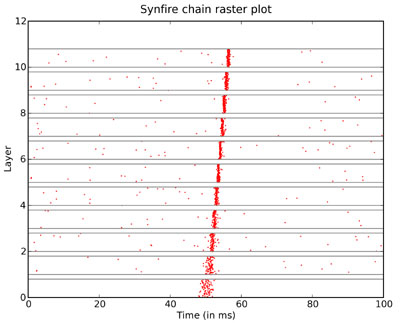
\includegraphics{synfirechain-example.jpg}

The simulation of 1000 neurons in 10 layers, each all-to-all connected to the next, using integrate and fire
neurons with synaptic noise for 100ms of simulated time took 1 second to run with a timestep of 0.1ms on a
2.4GHz Intel Xeon dual-core processor. The next image is of the state space, figure 3:

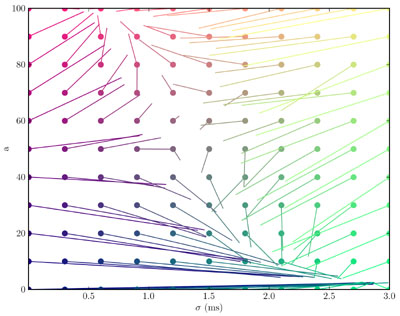
\includegraphics{sfc-statespace.jpg}

The figure computed 50 averages for each of 121 starting points over 100ms at a timestep of 0.1ms and took
201s to run on the same processor as above.

\resetcurrentobjects
\hypertarget{--doc-installation}{}

\chapter{Installation}

If you already have a copy of Python 2.5 or 2.6, try the Quick installation below,
otherwise take a look at Manual installation.


\section{Quick installation}

The easiest way to install Brian if you already have a version of Python 2.5 or 2.6 including the
\code{easy\_install} script is to simply run the following in a shell:

\begin{Verbatim}[commandchars=@\[\]]
easy@_install brian
\end{Verbatim}

This will download and install Brian and all its required packages (NumPy, SciPy, etc.).

Note that there are some optimisations you can make after installation, see the
section below on Optimisations.


\section{Manual installation}

Installing Brian requires the following components:
\begin{enumerate}
\item {} 
\href{http://www.python.org/download/}{Python} version 2.5 or 2.6.

\item {} 
\href{http://www.scipy.org/Download}{NumPy and Scipy} packages for Python:
an efficient scientific library.

\item {} 
\href{http://matplotlib.sourceforge.net/}{PyLab} package for Python:
a plotting library similar to Matlab
(see the \href{http://matplotlib.sourceforge.net/installing.html}{detailed installation instructions}).

\item {} 
\href{http://code.google.com/p/sympy/}{SymPy} package for Python:
a library for symbolic mathematics (not mandatory yet for Brian).

\item {} 
\href{http://neuralensemble.org/trac/brian/wiki/Downloads}{Brian} itself (don't forget to download the extras.zip file,
which includes examples, tutorials, and a complete copy of the documentation).
Brian is also a Python package and can be installed as explained below.

\end{enumerate}

Fortunately, Python packages are very quick and easy to install, so the whole process shouldn't
take very long.

We also recommend using the following for writing programs in Python (see details below):
\begin{enumerate}
\item {} 
\href{http://www.eclipse.org/}{Eclipse} IDE with \href{http://pydev.sourceforge.net/}{PyDev}

\item {} 
\href{http://ipython.scipy.org/moin/}{IPython} shell

\end{enumerate}

Finally, if you want to use the (optional) automatic C++ code generation features of Brian, you should
have the \code{gcc} compiler installed (on \href{http://www.cygwin.com/}{Cygwin} if you are
running on Windows).

Mac users: the \href{http://trichech.us/?page\_id=5}{Scipy Superpack for Intel OS X} includes
recent versions of Numpy, Scipy, Pylab and IPython.

Windows users: the \href{http://www.pythonxy.com/}{Python(x,y)} distribution includes all the packages
(including Eclipse and IPython) above except Brian (which is available as an optional plugin).


\subsection{Installing Python packages}

On Windows, Python packages (including Brian) are generally installed simply by running an .exe file.
On other operating systems, you can download the source release (typically a compressed
archive .tar.gz or .zip that you need to unzip) and then install the package by typing the following in your
shell:

\begin{Verbatim}[commandchars=@\[\]]
python setup.py install
\end{Verbatim}


\subsection{Installing Eclipse}

Eclipse is an Integrated Development Environment (IDE) for any programming language. PyDev is a plugin
for Eclipse with features specifically for Python development. The combination of these two is
excellent for Python development (it's what we use for writing Brian).

To install Eclipse, go to \href{http://www.eclipse.org/}{their web page} and download any of the base
language IDEs. It doesn't matter which one, but Python is not one of the base languages so you have
to choose an alternative language. Probably the most useful is the C++ one or the Java one. The C++
one can be downloaded \href{http://www.eclipse.org/cdt/downloads.php}{here}.

Having downloaded and installed Eclipse, you should download and install the PyDev plugin from
\href{http://pydev.sourceforge.net/}{their web site}. The best way to do this is directly from within
the Eclipse IDE. Follow the instructions on the \href{http://www.fabioz.com/pydev/manual\_101\_root.html}{PyDev manual page}.


\subsection{Installing IPython}

\href{http://ipython.scipy.org/moin/}{IPython} is an interactive shell for Python.
It has features for SciPy and PyLab built in, so it is a good choice for scientific work.
Download from \href{http://ipython.scipy.org/moin/Download}{their page}. If you are using Windows, you
will also need to download PyReadline from the same page.


\subsection{C++ compilers}

The default for Brian is to use the \code{gcc} compiler which will
be installed already on most unix or linux distributions. If you are using Windows, you can
install \href{http://www.cygwin.com/}{cygwin} (make sure to include the \code{gcc} package). Alternatively,
some but not all versions of Microsoft Visual C++ should be compatible, but this is untested
so far. See the documentation for the \href{http://www.scipy.org/Weave}{SciPy Weave} package for
more information on this. See also the section on \hyperlink{compiled-code}{\emph{Compiled code}}.


\section{Testing}

You can test whether Brian has installed properly by running Python and typing
the following two lines:

\begin{Verbatim}[commandchars=@\[\]]
@PYG[k+kn][from] @PYG[n+nn][brian] @PYG[k+kn][import] @PYG[o][*]
@PYG[n][brian@_sample@_run]@PYG[p][(]@PYG[p][)]
\end{Verbatim}

A sample network should run and produce a raster plot.


\section{Optimisations}

After a successful installation, there are some optimisations you can make to
your Brian installation to get it running faster using compiled C code. We do
not include these as standard because they do not work on all computers, and
we want Brian to install without problems on all computers. Note that including
all the optimisations can result in significant speed increases (around 30\%).

These optimisations are described in detail in the section on \hyperlink{compiled-code}{\emph{Compiled code}}.

\resetcurrentobjects
\hypertarget{--doc-slowstart}{}

\chapter{Getting started}

\resetcurrentobjects
\hypertarget{--doc-tutorials}{}

\section{Tutorials}

These tutorials cover some basic topics in writing Brian scripts in Python. The
complete source code for the tutorials is available in the tutorials folder
in the extras package.

\resetcurrentobjects
\hypertarget{--doc-othertutorials}{}

\subsection{Tutorials for Python and Scipy}


\subsubsection{Python}

The first thing to do in learning how to use Brian
is to have a basic grasp of the Python programming language.
There are lots of good tutorials already out there. The best one is probably
\href{http://docs.python.org/tut/}{the official Python tutorial}.
There is also a course for biologists at the Pasteur Institute:
\href{http://www.pasteur.fr/formation/infobio/python/}{Introduction to programming using Python}.


\subsubsection{NumPy, SciPy and Pylab}

The first place to look is the \href{http://docs.scipy.org/doc/}{SciPy documentation website}. To start using Brian, you do not need
to understand much about how NumPy and SciPy work, although understanding how their
array structures work will be useful for more advanced uses of Brian.

The syntax of the Numpy and Pylab functions is very similar to Matlab.
If you already know Matlab, you could read this tutorial:
\href{http://scipy.org/NumPy\_for\_Matlab\_Users}{NumPy for Matlab users}
and this list of \href{http://mathesaurus.sourceforge.net/}{Matlab-Python translations}
(\href{http://brian.di.ens.fr/matlab-python-xref.pdf}{pdf version here}).
A \href{http://matplotlib.sourceforge.net/users/pyplot\_tutorial.html}{tutorial} is also available on
the web site of Pylab.

\resetcurrentobjects
\hypertarget{--doc-tutorial1_basic_concepts}{}

\hypertarget{tutorial1-basic-concepts}{}\subsection{Tutorial 1: Basic Concepts}

In this tutorial, we introduce some of the basic concepts of a Brian simulation:
\begin{itemize}
\item {} 
Importing the Brian module into Python

\item {} 
Using quantities with units

\item {} 
Defining a neuron model by its differential equation

\item {} 
Creating a group of neurons

\item {} 
Running a network

\item {} 
Looking at the output of the network

\item {} 
Modifying the state variables of the network directly

\item {} 
Defining the network structure by connecting neurons

\item {} 
Doing a raster plot of the output

\item {} 
Plotting the membrane potential of an individual neuron

\end{itemize}

The following Brian classes will be introduced:
\begin{itemize}
\item {} 
\hyperlink{brian.NeuronGroup}{\code{NeuronGroup}}

\item {} 
\hyperlink{brian.Connection}{\code{Connection}}

\item {} 
\hyperlink{brian.SpikeMonitor}{\code{SpikeMonitor}}

\item {} 
\hyperlink{brian.StateMonitor}{\code{StateMonitor}}

\end{itemize}

We will build a Brian program that defines a randomly connected network of integrate
and fire neurons and plot its output.

This tutorial assumes you know:
\begin{itemize}
\item {} 
The very basics of Python, the \code{import} keyword, variables, basic
arithmetical expressions, calling functions, lists

\item {} 
The simplest leaky integrate and fire neuron model

\end{itemize}

The best place to start learning Python is the official tutorial:
\begin{quote}

\href{http://docs.python.org/tut/}{http://docs.python.org/tut/}
\end{quote}

\textbf{Tutorial contents}

\resetcurrentobjects
\hypertarget{--doc-tutorial_1a_the_simplest_brian_program}{}

\subsubsection{Tutorial 1a: The simplest Brian program}


\paragraph{Importing the Brian module}

The first thing to do in any Brian program is to load Brian and the names of
its functions and classes. The standard way to do this is to use the Python
\code{from ... import *} statement.
\begin{quote}

\begin{Verbatim}[commandchars=@\[\]]
@PYG[k+kn][from] @PYG[n+nn][brian] @PYG[k+kn][import] @PYG[o][*]
\end{Verbatim}
\end{quote}


\paragraph{Integrate and Fire model}

The neuron model we will use in this tutorial is the simplest possible
leaky integrate and fire neuron, defined by the differential equation:
\begin{quote}

tau dV/dt = -(V-El)
\end{quote}

and with a threshold value Vt and reset value Vr.


\paragraph{Parameters}

Brian has a system for defining physical quantities (quantities with
a physical dimension such as time). The code below illustrates how
to use this system, which (mostly) works just as you'd expect.
\begin{quote}

\begin{Verbatim}[commandchars=@\[\]]
@PYG[n][tau] @PYG[o][=] @PYG[l+m+mi][20]@PYG[o][*]@PYG[n][msecond]        @PYG[c][@# membrane time constant]
@PYG[n][Vt]  @PYG[o][=]@PYG[o][-]@PYG[l+m+mi][50]@PYG[o][*]@PYG[n][mvolt]          @PYG[c][@# spike threshold]
@PYG[n][Vr]  @PYG[o][=]@PYG[o][-]@PYG[l+m+mi][60]@PYG[o][*]@PYG[n][mvolt]          @PYG[c][@# reset value]
@PYG[n][El]  @PYG[o][=]@PYG[o][-]@PYG[l+m+mi][60]@PYG[o][*]@PYG[n][mvolt]          @PYG[c][@# resting potential (same as the reset)]
\end{Verbatim}
\end{quote}

The built in standard units in Brian consist of all the fundamental
SI units like second and metre, along with a selection of derived
SI units such as volt, farad, coulomb. All names are lowercase
following the SI standard. In addition, there are scaled versions
of these units using the standard SI prefixes m=1/1000, K=1000, etc.


\paragraph{Neuron model and equations}

The simplest way to define a neuron model in Brian is to write a list
of the differential equations that define it. For the moment, we'll just
give the simplest possible example, a single differential equation. You
write it in the following form:

\begin{Verbatim}[commandchars=@\[\]]
dx/dt = f(x) : unit
\end{Verbatim}

where \code{x} is the name of the variable, \code{f(x)} can be any valid Python
expression, and \code{unit} is the physical units of the variable \code{x}. In our
case we will write:

\begin{Verbatim}[commandchars=@\[\]]
dV/dt = -(V-El)/tau : volt
\end{Verbatim}

to define the variable \code{V} with units \code{volt}.

To complete the specification of the model, we also define a threshold and reset
value and create a group of 40 neurons with this model.
\begin{quote}

\begin{Verbatim}[commandchars=@\[\]]
@PYG[n][G] @PYG[o][=] @PYG[n][NeuronGroup]@PYG[p][(]@PYG[n][N]@PYG[o][=]@PYG[l+m+mi][40]@PYG[p][,] @PYG[n][model]@PYG[o][=]@PYG[l+s][']@PYG[l+s][dV/dt = -(V-El)/tau : volt]@PYG[l+s][']@PYG[p][,]
              @PYG[n][threshold]@PYG[o][=]@PYG[n][Vt]@PYG[p][,] @PYG[n][reset]@PYG[o][=]@PYG[n][Vr]@PYG[p][)]
\end{Verbatim}
\end{quote}

The statement creates a new object `G' which is an instance of the
Brian class \hyperlink{brian.NeuronGroup}{\code{NeuronGroup}}, initialised with the values in the
line above and 40 neurons. In Python, you can call a function or initialise
a class using keyword arguments as well as ordered arguments, so
if I defined a function \code{f(x,y)} I could call it as \code{f(1,2)} or
as \code{f(y=2,x=1)} and get the same effect. See the Python tutorial
for more information on this.

For the moment, we leave the neurons in this group unconnected
to each other, each evolves separately from the others.


\paragraph{Simulation}

Finally, we run the simulation for 1 second of simulated time.
By default, the simulator uses a timestep dt = 0.1 ms.
\begin{quote}

\begin{Verbatim}[commandchars=@\[\]]
@PYG[n][run]@PYG[p][(]@PYG[l+m+mi][1]@PYG[o][*]@PYG[n][second]@PYG[p][)]
\end{Verbatim}
\end{quote}

And that's it! To see some of the output of this network, go
to the next part of the tutorial.


\paragraph{Exercise}

The units system of Brian is useful for ensuring that everything
is consistent, and that you don't make hard to find mistakes in
your code by using the wrong units. Try changing the units of one
of the parameters and see what happens.


\paragraph{Solution}

You should see an error message with a Python traceback (telling
you which functions were being called when the error happened),
ending in a line something like:

\begin{Verbatim}[commandchars=@\[\]]
Brian.units.DimensionMismatchError: The differential equations
are not homogeneous!, dimensions were (m@textasciicircum[]2 kg s@textasciicircum[]-3 A@textasciicircum[]-1)
(m@textasciicircum[]2 kg s@textasciicircum[]-4 A@textasciicircum[]-1)
\end{Verbatim}

\resetcurrentobjects
\hypertarget{--doc-tutorial_1b_counting_spikes}{}

\subsubsection{Tutorial 1b: Counting spikes}

In the previous part of the tutorial we looked at the following:
\begin{itemize}
\item {} 
Importing the Brian module into Python

\item {} 
Using quantities with units

\item {} 
Defining a neuron model by its differential equation

\item {} 
Creating a group of neurons

\item {} 
Running a network

\end{itemize}

In this part, we move on to looking at the output of the network.

The first part of the code is the same.
\begin{quote}

\begin{Verbatim}[commandchars=@\[\]]
@PYG[k+kn][from] @PYG[n+nn][brian] @PYG[k+kn][import] @PYG[o][*]

@PYG[n][tau] @PYG[o][=] @PYG[l+m+mi][20]@PYG[o][*]@PYG[n][msecond]        @PYG[c][@# membrane time constant]
@PYG[n][Vt]  @PYG[o][=]@PYG[o][-]@PYG[l+m+mi][50]@PYG[o][*]@PYG[n][mvolt]          @PYG[c][@# spike threshold]
@PYG[n][Vr]  @PYG[o][=]@PYG[o][-]@PYG[l+m+mi][60]@PYG[o][*]@PYG[n][mvolt]          @PYG[c][@# reset value]
@PYG[n][El]  @PYG[o][=]@PYG[o][-]@PYG[l+m+mi][60]@PYG[o][*]@PYG[n][mvolt]          @PYG[c][@# resting potential (same as the reset)]

@PYG[n][G] @PYG[o][=] @PYG[n][NeuronGroup]@PYG[p][(]@PYG[n][N]@PYG[o][=]@PYG[l+m+mi][40]@PYG[p][,] @PYG[n][model]@PYG[o][=]@PYG[l+s][']@PYG[l+s][dV/dt = -(V-El)/tau : volt]@PYG[l+s][']@PYG[p][,]
              @PYG[n][threshold]@PYG[o][=]@PYG[n][Vt]@PYG[p][,] @PYG[n][reset]@PYG[o][=]@PYG[n][Vr]@PYG[p][)]
\end{Verbatim}
\end{quote}


\paragraph{Counting spikes}

Now we would like to have some idea of what this network is
doing. In Brian, we use monitors to keep track of the behaviour
of the network during the simulation. The simplest monitor of
all is the \hyperlink{brian.SpikeMonitor}{\code{SpikeMonitor}}, which just records the spikes from a
given \hyperlink{brian.NeuronGroup}{\code{NeuronGroup}}.
\begin{quote}

\begin{Verbatim}[commandchars=@\[\]]
@PYG[n][M] @PYG[o][=] @PYG[n][SpikeMonitor]@PYG[p][(]@PYG[n][G]@PYG[p][)]
\end{Verbatim}
\end{quote}


\paragraph{Results}

Now we run the simulation as before:
\begin{quote}

\begin{Verbatim}[commandchars=@\[\]]
@PYG[n][run]@PYG[p][(]@PYG[l+m+mi][1]@PYG[o][*]@PYG[n][second]@PYG[p][)]
\end{Verbatim}
\end{quote}

And finally, we print out how many spikes there were:
\begin{quote}

\begin{Verbatim}[commandchars=@\[\]]
@PYG[k][print] @PYG[n][M]@PYG[o][.]@PYG[n][nspikes]
\end{Verbatim}
\end{quote}

So what's going on? Why are there 40 spikes? Well, the answer is
that the initial value of the membrane potential for every neuron
is 0 mV, which is above the threshold potential of -50 mV and so there
is an initial spike at t=0 and then it resets to -60 mV and stays there,
below the threshold potential. In the next part of this tutorial, we'll
make sure there are some more spikes to see.

\resetcurrentobjects
\hypertarget{--doc-tutorial_1c_making_some_activity}{}

\subsubsection{Tutorial 1c: Making some activity}

In the previous part of the tutorial we found that each neuron
was producing only one spike. In this part, we alter the model so
that some more spikes will be generated. What we'll do is alter
the resting potential \code{El} so that it is above threshold, this
will ensure that some spikes are generated. The first few
lines remain the same:
\begin{quote}

\begin{Verbatim}[commandchars=@\[\]]
@PYG[k+kn][from] @PYG[n+nn][brian] @PYG[k+kn][import] @PYG[o][*]

@PYG[n][tau] @PYG[o][=] @PYG[l+m+mi][20]@PYG[o][*]@PYG[n][msecond]        @PYG[c][@# membrane time constant]
@PYG[n][Vt]  @PYG[o][=]@PYG[o][-]@PYG[l+m+mi][50]@PYG[o][*]@PYG[n][mvolt]          @PYG[c][@# spike threshold]
@PYG[n][Vr]  @PYG[o][=]@PYG[o][-]@PYG[l+m+mi][60]@PYG[o][*]@PYG[n][mvolt]          @PYG[c][@# reset value]
\end{Verbatim}
\end{quote}

But we change the resting potential to -49 mV, just above the
spike threshold:
\begin{quote}

\begin{Verbatim}[commandchars=@\[\]]
@PYG[n][El]  @PYG[o][=]@PYG[o][-]@PYG[l+m+mi][49]@PYG[o][*]@PYG[n][mvolt]          @PYG[c][@# resting potential (same as the reset)]
\end{Verbatim}
\end{quote}

And then continue as before:
\begin{quote}

\begin{Verbatim}[commandchars=@\[\]]
@PYG[n][G] @PYG[o][=] @PYG[n][NeuronGroup]@PYG[p][(]@PYG[n][N]@PYG[o][=]@PYG[l+m+mi][40]@PYG[p][,] @PYG[n][model]@PYG[o][=]@PYG[l+s][']@PYG[l+s][dV/dt = -(V-El)/tau : volt]@PYG[l+s][']@PYG[p][,]
              @PYG[n][threshold]@PYG[o][=]@PYG[n][Vt]@PYG[p][,] @PYG[n][reset]@PYG[o][=]@PYG[n][Vr]@PYG[p][)]

@PYG[n][M] @PYG[o][=] @PYG[n][SpikeMonitor]@PYG[p][(]@PYG[n][G]@PYG[p][)]

@PYG[n][run]@PYG[p][(]@PYG[l+m+mi][1]@PYG[o][*]@PYG[n][second]@PYG[p][)]

@PYG[k][print] @PYG[n][M]@PYG[o][.]@PYG[n][nspikes]
\end{Verbatim}
\end{quote}

Running this program gives the output \code{840}. That's because
every neuron starts at the same initial value and proceeds
deterministically, so that each neuron fires at exactly the
same time, in total 21 times during the 1s of the run.

In the next part, we'll introduce a random element into the
behaviour of the network.


\paragraph{Exercises}
\begin{enumerate}
\item {} 
Try varying the parameters and seeing how the number of
spikes generated varies.

\item {} 
Solve the differential equation by hand and compute a
formula for the number of spikes generated. Compare this
with the program output and thereby partially verify it.
(Hint: each neuron starts at above the threshold and so
fires a spike immediately.)

\end{enumerate}


\paragraph{Solution}

Solving the differential equation gives:
\begin{quote}

V = El + (Vr-El) exp (-t/tau)
\end{quote}

Setting V=Vt at time t gives:
\begin{quote}

t = tau log( (Vr-El) / (Vt-El) )
\end{quote}

If the simulator runs for time T, and fires a spike immediately
at the beginning of the run it will then generate n spikes,
where:
\begin{quote}

n = {[}T/t{]} + 1
\end{quote}

If you have m neurons all doing the same thing, you get nm
spikes. This calculation with the parameters above gives:
\begin{quote}

t = 48.0 ms
n = 21
nm = 840
\end{quote}

As predicted.

\resetcurrentobjects
\hypertarget{--doc-tutorial_1d_introducing_randomness}{}

\subsubsection{Tutorial 1d: Introducing randomness}

In the previous part of the tutorial, all the neurons start
at the same values and proceed deterministically, so they all
spike at exactly the same times. In this part, we introduce
some randomness by initialising all the membrane potentials
to uniform random values between the reset and threshold
values.

We start as before:
\begin{quote}

\begin{Verbatim}[commandchars=@\[\]]
@PYG[k+kn][from] @PYG[n+nn][brian] @PYG[k+kn][import] @PYG[o][*]

@PYG[n][tau] @PYG[o][=] @PYG[l+m+mi][20]@PYG[o][*]@PYG[n][msecond]        @PYG[c][@# membrane time constant]
@PYG[n][Vt]  @PYG[o][=]@PYG[o][-]@PYG[l+m+mi][50]@PYG[o][*]@PYG[n][mvolt]          @PYG[c][@# spike threshold]
@PYG[n][Vr]  @PYG[o][=]@PYG[o][-]@PYG[l+m+mi][60]@PYG[o][*]@PYG[n][mvolt]          @PYG[c][@# reset value]
@PYG[n][El]  @PYG[o][=]@PYG[o][-]@PYG[l+m+mi][49]@PYG[o][*]@PYG[n][mvolt]          @PYG[c][@# resting potential (same as the reset)]

@PYG[n][G] @PYG[o][=] @PYG[n][NeuronGroup]@PYG[p][(]@PYG[n][N]@PYG[o][=]@PYG[l+m+mi][40]@PYG[p][,] @PYG[n][model]@PYG[o][=]@PYG[l+s][']@PYG[l+s][dV/dt = -(V-El)/tau : volt]@PYG[l+s][']@PYG[p][,]
              @PYG[n][threshold]@PYG[o][=]@PYG[n][Vt]@PYG[p][,] @PYG[n][reset]@PYG[o][=]@PYG[n][Vr]@PYG[p][)]

@PYG[n][M] @PYG[o][=] @PYG[n][SpikeMonitor]@PYG[p][(]@PYG[n][G]@PYG[p][)]
\end{Verbatim}
\end{quote}

But before we run the simulation, we set the values of the
membrane potentials directly. The notation \code{G.V} refers
to the array of values for the variable \code{V} in group \code{G}. In
our case, this is an array of length 40. We set its values
by generating an array of random numbers using Brian's
\code{rand} function. The syntax is \code{rand(size)} generates an
array of length \code{size} consisting of uniformly distributed
random numbers in the interval 0, 1.
\begin{quote}

\begin{Verbatim}[commandchars=@\[\]]
@PYG[n][G]@PYG[o][.]@PYG[n][V]@PYG[o][=]@PYG[n][Vr]@PYG[o][+]@PYG[n][rand]@PYG[p][(]@PYG[l+m+mi][40]@PYG[p][)]@PYG[o][*]@PYG[p][(]@PYG[n][Vt]@PYG[o][-]@PYG[n][Vr]@PYG[p][)]
\end{Verbatim}
\end{quote}

And now we run the simulation as before.
\begin{quote}

\begin{Verbatim}[commandchars=@\[\]]
@PYG[n][run]@PYG[p][(]@PYG[l+m+mi][1]@PYG[o][*]@PYG[n][second]@PYG[p][)]

@PYG[k][print] @PYG[n][M]@PYG[o][.]@PYG[n][nspikes]
\end{Verbatim}
\end{quote}

But this time we get a varying number of spikes each time
we run it, roughly between 800 and 850 spikes. In the
next part of this tutorial, we introduce a bit more
interest into this network by connecting the neurons together.

\resetcurrentobjects
\hypertarget{--doc-tutorial_1e_connecting_neurons}{}

\subsubsection{Tutorial 1e: Connecting neurons}

In the previous parts of this tutorial, the neurons are
still all unconnected. We add in connections here. The
model we use is that when neuron i is connected to
neuron j and neuron i fires a spike, then the membrane
potential of neuron j is instantaneously increased by
a value \code{psp}. We start as before:
\begin{quote}

\begin{Verbatim}[commandchars=@\[\]]
@PYG[k+kn][from] @PYG[n+nn][brian] @PYG[k+kn][import] @PYG[o][*]

@PYG[n][tau] @PYG[o][=] @PYG[l+m+mi][20]@PYG[o][*]@PYG[n][msecond]        @PYG[c][@# membrane time constant]
@PYG[n][Vt]  @PYG[o][=]@PYG[o][-]@PYG[l+m+mi][50]@PYG[o][*]@PYG[n][mvolt]          @PYG[c][@# spike threshold]
@PYG[n][Vr]  @PYG[o][=]@PYG[o][-]@PYG[l+m+mi][60]@PYG[o][*]@PYG[n][mvolt]          @PYG[c][@# reset value]
@PYG[n][El]  @PYG[o][=]@PYG[o][-]@PYG[l+m+mi][49]@PYG[o][*]@PYG[n][mvolt]          @PYG[c][@# resting potential (same as the reset)]
\end{Verbatim}
\end{quote}

Now we include a new parameter, the PSP size:
\begin{quote}

\begin{Verbatim}[commandchars=@\[\]]
@PYG[n][psp] @PYG[o][=] @PYG[l+m+mf][0.5]@PYG[o][*]@PYG[n][mvolt]         @PYG[c][@# postsynaptic potential size]
\end{Verbatim}
\end{quote}

And continue as before:
\begin{quote}

\begin{Verbatim}[commandchars=@\[\]]
@PYG[n][G] @PYG[o][=] @PYG[n][NeuronGroup]@PYG[p][(]@PYG[n][N]@PYG[o][=]@PYG[l+m+mi][40]@PYG[p][,] @PYG[n][model]@PYG[o][=]@PYG[l+s][']@PYG[l+s][dV/dt = -(V-El)/tau : volt]@PYG[l+s][']@PYG[p][,]
              @PYG[n][threshold]@PYG[o][=]@PYG[n][Vt]@PYG[p][,] @PYG[n][reset]@PYG[o][=]@PYG[n][Vr]@PYG[p][)]
\end{Verbatim}
\end{quote}


\paragraph{Connections}

We now proceed to connect these neurons. Firstly, we declare
that there is a connection from neurons in \code{G} to neurons in \code{G}.
For the moment, this is just something that is necessary to
do, the reason for doing it this way will become clear in the
next tutorial.
\begin{quote}

\begin{Verbatim}[commandchars=@\[\]]
@PYG[n][C] @PYG[o][=] @PYG[n][Connection]@PYG[p][(]@PYG[n][G]@PYG[p][,]@PYG[n][G]@PYG[p][)]
\end{Verbatim}
\end{quote}

Now the interesting part, we make these neurons be randomly
connected with probability 0.1 and weight \code{psp}. Each neuron
i in \code{G} will be connected to each neuron j in \code{G}
with probability 0.1. The weight of the connection is the
amount that is added to the membrane potential of the target
neuron when the source neuron fires a spike.
\begin{quote}

\begin{Verbatim}[commandchars=@\[\]]
@PYG[n][C]@PYG[o][.]@PYG[n][connect@_random]@PYG[p][(]@PYG[n][sparseness]@PYG[o][=]@PYG[l+m+mf][0.1]@PYG[p][,]@PYG[n][weight]@PYG[o][=]@PYG[n][psp]@PYG[p][)]
\end{Verbatim}
\end{quote}

These two previous lines could be done in one line:

\begin{Verbatim}[commandchars=@\[\]]
@PYG[n][C] @PYG[o][=] @PYG[n][Connection]@PYG[p][(]@PYG[n][G]@PYG[p][,]@PYG[n][G]@PYG[p][,]@PYG[n][sparseness]@PYG[o][=]@PYG[l+m+mf][0.1]@PYG[p][,]@PYG[n][weight]@PYG[o][=]@PYG[n][psp]@PYG[p][)]
\end{Verbatim}

Now we continue as before:
\begin{quote}

\begin{Verbatim}[commandchars=@\[\]]
@PYG[n][M] @PYG[o][=] @PYG[n][SpikeMonitor]@PYG[p][(]@PYG[n][G]@PYG[p][)]

@PYG[n][G]@PYG[o][.]@PYG[n][V]@PYG[o][=]@PYG[n][Vr]@PYG[o][+]@PYG[n][rand]@PYG[p][(]@PYG[l+m+mi][40]@PYG[p][)]@PYG[o][*]@PYG[p][(]@PYG[n][Vt]@PYG[o][-]@PYG[n][Vr]@PYG[p][)]

@PYG[n][run]@PYG[p][(]@PYG[l+m+mi][1]@PYG[o][*]@PYG[n][second]@PYG[p][)]

@PYG[k][print] @PYG[n][M]@PYG[o][.]@PYG[n][nspikes]
\end{Verbatim}
\end{quote}

You can see that the number of spikes has jumped from around
800-850 to around 1000-1200. In the next part of the tutorial,
we'll look at a way to plot the output of the network.


\paragraph{Exercise}

Try varying the parameter \code{psp} and see what happens. How large
can you make the number of spikes output by the network? Why?


\paragraph{Solution}

The logically maximum number of firings is
400,000 = 40 * 1000 / 0.1, the number of neurons in the
network * the time it runs for / the integration step size (you
cannot have more than one spike per step).

In fact, the number of firings is bounded above by 200,000. The
reason for this is that the network updates in the following way:
\begin{enumerate}
\item {} 
Integration step

\item {} 
Find neurons above threshold

\item {} 
Propagate spikes

\item {} 
Reset neurons which spiked

\end{enumerate}

You can see then that if neuron i has spiked at time t, then it
will not spike at time t+dt, even if it receives spikes from
another neuron. Those spikes it receives will be added at step
3 at time t, then reset to \code{Vr} at step 4 of time t, then the
thresholding function at time t+dt is applied at step 2, before
it has received any subsequent inputs. So the most a neuron
can spike is every other time step.

\resetcurrentobjects
\hypertarget{--doc-tutorial_1f_recording_spikes}{}

\subsubsection{Tutorial 1f: Recording spikes}

In the previous part of the tutorial, we defined a network with
not entirely trivial behaviour, and printed the number of spikes.
In this part, we'll record every spike that the network generates
and display a raster plot of them. We start as before:
\begin{quote}

\begin{Verbatim}[commandchars=@\[\]]
@PYG[k+kn][from] @PYG[n+nn][brian] @PYG[k+kn][import] @PYG[o][*]

@PYG[n][tau] @PYG[o][=] @PYG[l+m+mi][20]@PYG[o][*]@PYG[n][msecond]        @PYG[c][@# membrane time constant]
@PYG[n][Vt]  @PYG[o][=]@PYG[o][-]@PYG[l+m+mi][50]@PYG[o][*]@PYG[n][mvolt]          @PYG[c][@# spike threshold]
@PYG[n][Vr]  @PYG[o][=]@PYG[o][-]@PYG[l+m+mi][60]@PYG[o][*]@PYG[n][mvolt]          @PYG[c][@# reset value]
@PYG[n][El]  @PYG[o][=]@PYG[o][-]@PYG[l+m+mi][49]@PYG[o][*]@PYG[n][mvolt]          @PYG[c][@# resting potential (same as the reset)]
@PYG[n][psp] @PYG[o][=] @PYG[l+m+mf][0.5]@PYG[o][*]@PYG[n][mvolt]         @PYG[c][@# postsynaptic potential size]

@PYG[n][G] @PYG[o][=] @PYG[n][NeuronGroup]@PYG[p][(]@PYG[n][N]@PYG[o][=]@PYG[l+m+mi][40]@PYG[p][,] @PYG[n][model]@PYG[o][=]@PYG[l+s][']@PYG[l+s][dV/dt = -(V-El)/tau : volt]@PYG[l+s][']@PYG[p][,]
              @PYG[n][threshold]@PYG[o][=]@PYG[n][Vt]@PYG[p][,] @PYG[n][reset]@PYG[o][=]@PYG[n][Vr]@PYG[p][)]

@PYG[n][C] @PYG[o][=] @PYG[n][Connection]@PYG[p][(]@PYG[n][G]@PYG[p][,]@PYG[n][G]@PYG[p][)]
@PYG[n][C]@PYG[o][.]@PYG[n][connect@_random]@PYG[p][(]@PYG[n][sparseness]@PYG[o][=]@PYG[l+m+mf][0.1]@PYG[p][,]@PYG[n][weight]@PYG[o][=]@PYG[n][psp]@PYG[p][)]

@PYG[n][M] @PYG[o][=] @PYG[n][SpikeMonitor]@PYG[p][(]@PYG[n][G]@PYG[p][)]

@PYG[n][G]@PYG[o][.]@PYG[n][V]@PYG[o][=]@PYG[n][Vr]@PYG[o][+]@PYG[n][rand]@PYG[p][(]@PYG[l+m+mi][40]@PYG[p][)]@PYG[o][*]@PYG[p][(]@PYG[n][Vt]@PYG[o][-]@PYG[n][Vr]@PYG[p][)]

@PYG[n][run]@PYG[p][(]@PYG[l+m+mi][1]@PYG[o][*]@PYG[n][second]@PYG[p][)]

@PYG[k][print] @PYG[n][M]@PYG[o][.]@PYG[n][nspikes]
\end{Verbatim}
\end{quote}

Having run the network, we simply use the \hyperlink{brian.raster_plot}{\code{raster\_plot()}} function
provided by Brian. After creating plots, we have to use the
\code{show()} function to display them. This function is from the
PyLab module that Brian uses for its built in plotting
routines.
\begin{quote}

\begin{Verbatim}[commandchars=@\[\]]
@PYG[n][raster@_plot]@PYG[p][(]@PYG[p][)]
@PYG[n][show]@PYG[p][(]@PYG[p][)]
\end{Verbatim}
\end{quote}

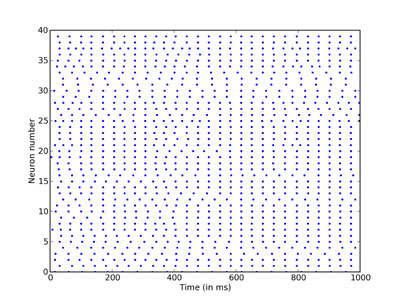
\includegraphics{1f.jpg}

As you can see, despite having introduced some randomness into
our network, the output is very regular indeed. In the next part
we introduce one more way to plot the output of a network.

\resetcurrentobjects
\hypertarget{--doc-tutorial_1g_recording_membrane_potentials}{}

\subsubsection{Tutorial 1g: Recording membrane potentials}

In the previous part of this tutorial, we plotted a raster plot of
the firing times of the network. In this tutorial, we introduce
a way to record the value of the membrane potential for a neuron
during the simulation, and plot it. We continue as before:
\begin{quote}

\begin{Verbatim}[commandchars=@\[\]]
@PYG[k+kn][from] @PYG[n+nn][brian] @PYG[k+kn][import] @PYG[o][*]

@PYG[n][tau] @PYG[o][=] @PYG[l+m+mi][20]@PYG[o][*]@PYG[n][msecond]        @PYG[c][@# membrane time constant]
@PYG[n][Vt]  @PYG[o][=]@PYG[o][-]@PYG[l+m+mi][50]@PYG[o][*]@PYG[n][mvolt]          @PYG[c][@# spike threshold]
@PYG[n][Vr]  @PYG[o][=]@PYG[o][-]@PYG[l+m+mi][60]@PYG[o][*]@PYG[n][mvolt]          @PYG[c][@# reset value]
@PYG[n][El]  @PYG[o][=]@PYG[o][-]@PYG[l+m+mi][49]@PYG[o][*]@PYG[n][mvolt]          @PYG[c][@# resting potential (same as the reset)]
@PYG[n][psp] @PYG[o][=] @PYG[l+m+mf][0.5]@PYG[o][*]@PYG[n][mvolt]         @PYG[c][@# postsynaptic potential size]

@PYG[n][G] @PYG[o][=] @PYG[n][NeuronGroup]@PYG[p][(]@PYG[n][N]@PYG[o][=]@PYG[l+m+mi][40]@PYG[p][,] @PYG[n][model]@PYG[o][=]@PYG[l+s][']@PYG[l+s][dV/dt = -(V-El)/tau : volt]@PYG[l+s][']@PYG[p][,]
              @PYG[n][threshold]@PYG[o][=]@PYG[n][Vt]@PYG[p][,] @PYG[n][reset]@PYG[o][=]@PYG[n][Vr]@PYG[p][)]

@PYG[n][C] @PYG[o][=] @PYG[n][Connection]@PYG[p][(]@PYG[n][G]@PYG[p][,]@PYG[n][G]@PYG[p][)]
@PYG[n][C]@PYG[o][.]@PYG[n][connect@_random]@PYG[p][(]@PYG[n][sparseness]@PYG[o][=]@PYG[l+m+mf][0.1]@PYG[p][,]@PYG[n][weight]@PYG[o][=]@PYG[n][psp]@PYG[p][)]
\end{Verbatim}
\end{quote}

This time we won't record the spikes.


\paragraph{Recording states}

Now we introduce a second type of monitor, the \hyperlink{brian.StateMonitor}{\code{StateMonitor}}.
The first argument is the group to monitor, and the second is
the state variable to monitor. The keyword \code{record} can be
an integer, list or the value \code{True}. If it is an integer \code{i},
the monitor will record the state of the variable for neuron \code{i}.
If it's a list of integers, it will record the states for
each neuron in the list. If it's set to \code{True} it will record
for all the neurons in the group.
\begin{quote}

\begin{Verbatim}[commandchars=@\[\]]
@PYG[n][M] @PYG[o][=] @PYG[n][StateMonitor]@PYG[p][(]@PYG[n][G]@PYG[p][,]@PYG[l+s][']@PYG[l+s][V]@PYG[l+s][']@PYG[p][,]@PYG[n][record]@PYG[o][=]@PYG[l+m+mi][0]@PYG[p][)]
\end{Verbatim}
\end{quote}

And then we continue as before:
\begin{quote}

\begin{Verbatim}[commandchars=@\[\]]
@PYG[n][G]@PYG[o][.]@PYG[n][V]@PYG[o][=]@PYG[n][Vr]@PYG[o][+]@PYG[n][rand]@PYG[p][(]@PYG[l+m+mi][40]@PYG[p][)]@PYG[o][*]@PYG[p][(]@PYG[n][Vt]@PYG[o][-]@PYG[n][Vr]@PYG[p][)]
\end{Verbatim}
\end{quote}

But this time we run it for a shorter time so we can look at
the output in more detail:
\begin{quote}

\begin{Verbatim}[commandchars=@\[\]]
@PYG[n][run]@PYG[p][(]@PYG[l+m+mi][200]@PYG[o][*]@PYG[n][msecond]@PYG[p][)]
\end{Verbatim}
\end{quote}

Having run the simulation, we plot the results using the
\code{plot} command from PyLab which has the same syntax as the Matlab
\code{plot{}`} command, i.e. \code{plot(xvals,yvals,...)}. The \hyperlink{brian.StateMonitor}{\code{StateMonitor}}
monitors the times at which it monitored a value in the
array \code{M.times}, and the values in the array \code{M{[}0{]}}. The notation
\code{M{[}i{]}} means the array of values of the monitored state
variable for neuron \code{i}.

In the following lines, we scale the times so that they're
measured in ms and the values so that they're measured in
mV. We also label the plot using PyLab's \code{xlabel}, \code{ylabel} and
\code{title} functions, which again mimic the Matlab equivalents.
\begin{quote}

\begin{Verbatim}[commandchars=@\[\]]
@PYG[n][plot]@PYG[p][(]@PYG[n][M]@PYG[o][.]@PYG[n][times]@PYG[o][/]@PYG[n][ms]@PYG[p][,]@PYG[n][M]@PYG[p][@PYGZlb[]]@PYG[l+m+mi][0]@PYG[p][@PYGZrb[]]@PYG[o][/]@PYG[n][mV]@PYG[p][)]
@PYG[n][xlabel]@PYG[p][(]@PYG[l+s][']@PYG[l+s][Time (in ms)]@PYG[l+s][']@PYG[p][)]
@PYG[n][ylabel]@PYG[p][(]@PYG[l+s][']@PYG[l+s][Membrane potential (in mV)]@PYG[l+s][']@PYG[p][)]
@PYG[n][title]@PYG[p][(]@PYG[l+s][']@PYG[l+s][Membrane potential for neuron 0]@PYG[l+s][']@PYG[p][)]
@PYG[n][show]@PYG[p][(]@PYG[p][)]
\end{Verbatim}
\end{quote}

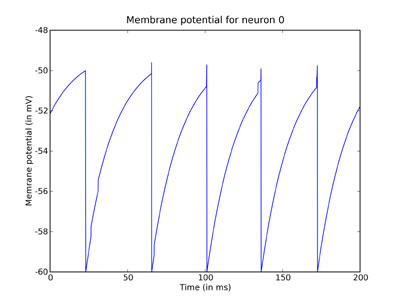
\includegraphics{1g.jpg}

You can clearly see the leaky integration exponential decay
toward the resting potential, as well as the jumps when a
spike was received.

\resetcurrentobjects
\hypertarget{--doc-tutorial2_connections}{}

\hypertarget{tutorial2-connections}{}\subsection{Tutorial 2: Connections}

In this tutorial, we will cover in more detail the concept of a \hyperlink{brian.Connection}{\code{Connection}}
in Brian.

\textbf{Tutorial contents}

\resetcurrentobjects
\hypertarget{--doc-tutorial_2a_the_concept_of_a_connection}{}

\subsubsection{Tutorial 2a: The concept of a Connection}


\paragraph{The network}

In this first part, we'll build a network consisting of three neurons. The
first two neurons will be under direct control and have no equations
defining them, they'll just produce spikes which will feed into the third
neuron. This third neuron has two different state variables, called Va
and Vb. The first two neurons will be connected to the third neuron, but
a spike arriving at the third neuron will be treated differently
according to whether it came from the first or second neuron (which you
can consider as meaning that the first two neurons have different
types of synapses on to the third neuron).

The program starts as follows.
\begin{quote}

\begin{Verbatim}[commandchars=@\[\]]
@PYG[k+kn][from] @PYG[n+nn][brian] @PYG[k+kn][import] @PYG[o][*]

@PYG[n][tau@_a] @PYG[o][=]  @PYG[l+m+mi][1]@PYG[o][*]@PYG[n][ms]
@PYG[n][tau@_b] @PYG[o][=] @PYG[l+m+mi][10]@PYG[o][*]@PYG[n][ms]
@PYG[n][Vt]    @PYG[o][=] @PYG[l+m+mi][10]@PYG[o][*]@PYG[n][mV]
@PYG[n][Vr]    @PYG[o][=]  @PYG[l+m+mi][0]@PYG[o][*]@PYG[n][mV]
\end{Verbatim}
\end{quote}


\paragraph{Differential equations}

This time, we will have multiple differential equations. We will use the
\hyperlink{brian.Equations}{\code{Equations}} object, although you could equally pass the multi-line string
defining the differential equations directly when initialising the \hyperlink{brian.NeuronGroup}{\code{NeuronGroup}}
object (see the next part of the tutorial for an example of this).
\begin{quote}

\begin{Verbatim}[commandchars=@\[\]]
@PYG[n][eqs] @PYG[o][=] @PYG[n][Equations]@PYG[p][(]@PYG[l+s][''']
@PYG[l+s][      dVa/dt = -Va/tau@_a : volt]
@PYG[l+s][      dVb/dt = -Vb/tau@_b : volt]
@PYG[l+s][      ]@PYG[l+s][''']@PYG[p][)]
\end{Verbatim}
\end{quote}

So far, we have defined a model neuron with two state variables, \code{Va}
and \code{Vb}, which both decay exponentially towards 0, but with different
time constants \code{tau\_a} and \code{tau\_b}. This is just so that you can see
the difference between them more clearly in the plot later on.


\paragraph{SpikeGeneratorGroup}

Now we introduce the \hyperlink{brian.SpikeGeneratorGroup}{\code{SpikeGeneratorGroup}} class. This is a group of
neurons without a model, which just produces spikes at the times
that you specify. You create a group like this by writing:

\begin{Verbatim}[commandchars=@\[\]]
@PYG[n][G] @PYG[o][=] @PYG[n][SpikeGeneratorGroup]@PYG[p][(]@PYG[n][N]@PYG[p][,]@PYG[n][spiketimes]@PYG[p][)]
\end{Verbatim}

where \code{N} is the number of neurons in the group, and \code{spiketimes} is a
list of pairs \code{(i,t)} indicating that neuron \code{i} should fire at time \code{t}.
In fact, \code{spiketimes} can be any `iterable container' or `generator',
but we don't cover that here (see the detailed documentation for
\hyperlink{brian.SpikeGeneratorGroup}{\code{SpikeGeneratorGroup}}).

In our case, we want to create a group with two neurons, the first
of which (neuron 0) fires at times 1 ms and 4 ms, and the second
of which (neuron 1) fires at times 2 ms and 3 ms. The list of
\code{spiketimes} then is:
\begin{quote}

\begin{Verbatim}[commandchars=@\[\]]
@PYG[n][spiketimes] @PYG[o][=] @PYG[p][@PYGZlb[]]@PYG[p][(]@PYG[l+m+mi][0]@PYG[p][,]@PYG[l+m+mi][1]@PYG[o][*]@PYG[n][ms]@PYG[p][)]@PYG[p][,] @PYG[p][(]@PYG[l+m+mi][0]@PYG[p][,]@PYG[l+m+mi][4]@PYG[o][*]@PYG[n][ms]@PYG[p][)]@PYG[p][,]
              @PYG[p][(]@PYG[l+m+mi][1]@PYG[p][,]@PYG[l+m+mi][2]@PYG[o][*]@PYG[n][ms]@PYG[p][)]@PYG[p][,] @PYG[p][(]@PYG[l+m+mi][1]@PYG[p][,]@PYG[l+m+mi][3]@PYG[o][*]@PYG[n][ms]@PYG[p][)]@PYG[p][@PYGZrb[]]
\end{Verbatim}
\end{quote}

and we create the group as follows:
\begin{quote}

\begin{Verbatim}[commandchars=@\[\]]
@PYG[n][G1] @PYG[o][=] @PYG[n][SpikeGeneratorGroup]@PYG[p][(]@PYG[l+m+mi][2]@PYG[p][,]@PYG[n][spiketimes]@PYG[p][)]
\end{Verbatim}
\end{quote}

Now we create a second group, with one neuron, according to the
model we defined earlier.
\begin{quote}

\begin{Verbatim}[commandchars=@\[\]]
@PYG[n][G2] @PYG[o][=] @PYG[n][NeuronGroup]@PYG[p][(]@PYG[n][N]@PYG[o][=]@PYG[l+m+mi][1]@PYG[p][,] @PYG[n][model]@PYG[o][=]@PYG[n][eqs]@PYG[p][,] @PYG[n][threshold]@PYG[o][=]@PYG[n][Vt]@PYG[p][,] @PYG[n][reset]@PYG[o][=]@PYG[n][Vr]@PYG[p][)]
\end{Verbatim}
\end{quote}


\paragraph{Connections}

In Brian, a \hyperlink{brian.Connection}{\code{Connection}} from one \hyperlink{brian.NeuronGroup}{\code{NeuronGroup}} to another is
defined by writing:

\begin{Verbatim}[commandchars=@\[\]]
@PYG[n][C] @PYG[o][=] @PYG[n][Connection]@PYG[p][(]@PYG[n][G]@PYG[p][,]@PYG[n][H]@PYG[p][,]@PYG[n][state]@PYG[p][)]
\end{Verbatim}

Here \code{G} is the source group, \code{H} is the target group, and \code{state} is the
name of the target state variable. When a neuron \code{i} in \code{G} fires, Brian
finds all the neurons \code{j} in \code{H} that \code{i} in \code{G} is connected to, and adds
the amount \code{C{[}i,j{]}} to the specified state variable of neuron \code{j} in \code{H}.
Here \code{C{[}i,j{]}} is the (i,j)th entry of the connection matrix of \code{C} (which
is initially all zero).

To start with, we create two connections from the group of two
directly controlled neurons to the group of one neuron with the
differential equations. The first connection has the target state \code{Va}
and the second has the target state \code{Vb}.
\begin{quote}

\begin{Verbatim}[commandchars=@\[\]]
@PYG[n][C1] @PYG[o][=] @PYG[n][Connection]@PYG[p][(]@PYG[n][G1]@PYG[p][,]@PYG[n][G2]@PYG[p][,]@PYG[l+s][']@PYG[l+s][Va]@PYG[l+s][']@PYG[p][)]
@PYG[n][C2] @PYG[o][=] @PYG[n][Connection]@PYG[p][(]@PYG[n][G1]@PYG[p][,]@PYG[n][G2]@PYG[p][,]@PYG[l+s][']@PYG[l+s][Vb]@PYG[l+s][']@PYG[p][)]
\end{Verbatim}
\end{quote}

So far, this only declares our intention to connect neurons in group
\code{G1} to neurons in group \code{G2}, because the connection matrix is initially
all zeros. Now, with connection \code{C1} we connect neuron 0 in group \code{G1}
to neuron 0 in group \code{G2}, with weight 3 mV. This means that when neuron
0 in group \code{G1} fires, the state variable \code{Va} of the neuron in group \code{G2}
will be increased by 6 mV. Then we use connection \code{C2} to connection
neuron 1 in group \code{G1} to neuron 0 in group \code{G2}, this time with weight
3 mV.
\begin{quote}

\begin{Verbatim}[commandchars=@\[\]]
@PYG[n][C1]@PYG[p][@PYGZlb[]]@PYG[l+m+mi][0]@PYG[p][,]@PYG[l+m+mi][0]@PYG[p][@PYGZrb[]] @PYG[o][=] @PYG[l+m+mi][6]@PYG[o][*]@PYG[n][mV]
@PYG[n][C2]@PYG[p][@PYGZlb[]]@PYG[l+m+mi][1]@PYG[p][,]@PYG[l+m+mi][0]@PYG[p][@PYGZrb[]] @PYG[o][=] @PYG[l+m+mi][3]@PYG[o][*]@PYG[n][mV]
\end{Verbatim}
\end{quote}

The net effect of this is that when neuron 0 of \code{G1} fires, \code{Va} for
the neuron in \code{G2} will increase 6 mV, and when neuron 1 of \code{G1} fires,
\code{Vb} for the neuron in \code{G2} will increase 3 mV.

Now we set up monitors to record the activity of the network,
run it and plot it.
\begin{quote}

\begin{Verbatim}[commandchars=@\[\]]
@PYG[n][Ma] @PYG[o][=] @PYG[n][StateMonitor]@PYG[p][(]@PYG[n][G2]@PYG[p][,]@PYG[l+s][']@PYG[l+s][Va]@PYG[l+s][']@PYG[p][,]@PYG[n][record]@PYG[o][=]@PYG[n+nb+bp][True]@PYG[p][)]
@PYG[n][Mb] @PYG[o][=] @PYG[n][StateMonitor]@PYG[p][(]@PYG[n][G2]@PYG[p][,]@PYG[l+s][']@PYG[l+s][Vb]@PYG[l+s][']@PYG[p][,]@PYG[n][record]@PYG[o][=]@PYG[n+nb+bp][True]@PYG[p][)]

@PYG[n][run]@PYG[p][(]@PYG[l+m+mi][10]@PYG[o][*]@PYG[n][ms]@PYG[p][)]

@PYG[n][plot]@PYG[p][(]@PYG[n][Ma]@PYG[o][.]@PYG[n][times]@PYG[p][,]@PYG[n][Ma]@PYG[p][@PYGZlb[]]@PYG[l+m+mi][0]@PYG[p][@PYGZrb[]]@PYG[p][)]
@PYG[n][plot]@PYG[p][(]@PYG[n][Mb]@PYG[o][.]@PYG[n][times]@PYG[p][,]@PYG[n][Mb]@PYG[p][@PYGZlb[]]@PYG[l+m+mi][0]@PYG[p][@PYGZrb[]]@PYG[p][)]
@PYG[n][show]@PYG[p][(]@PYG[p][)]
\end{Verbatim}
\end{quote}

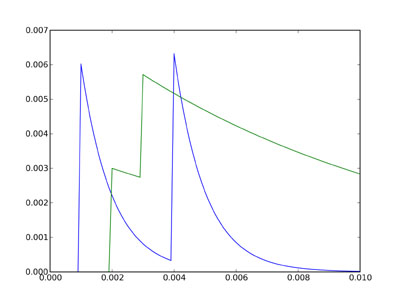
\includegraphics{2a.jpg}

The two plots show the state variables \code{Va} and \code{Vb} for the single
neuron in group \code{G2}. \code{Va} is shown in blue, and \code{Vb} in green.
According to the differential equations, \code{Va} decays much faster
than \code{Vb} (time constant 1 ms rather than 10 ms), but we have set
it up (through the connection strengths) that an incoming
spike from neuron 0 of \code{G1} causes a large increase of 6 mV to \code{Va},
whereas a spike from neuron 1 of \code{G1} causes a smaller increase of
3 mV to Vb. The value for \code{Va} then jumps at times 1 ms and 4 ms,
when we defined neuron 0 of \code{G1} to fire, and decays almost back
to rest in between. The value for \code{Vb} jumps at times 2 ms and
3 ms, and because the times are closer together and the time
constant is longer, they add together.

In the next part of this tutorial, we'll see how to use this
system to do something useful.


\paragraph{Exercises}
\begin{enumerate}
\item {} 
Try playing with the parameters \code{tau\_a}, \code{tau\_b} and the connection
strengths, \code{C1{[}0,0{]}} and \code{C2{[}0,1{]}}. Try changing the list of
spike times.

\item {} 
In this part of the tutorial, the states \code{Va} and \code{Vb} are
independent of one another. Try rewriting the differential
equations so that they're not independent and play around
with that.

\item {} 
Write a network with inhibitory and excitatory neurons. Hint: you
only need one connection.

\item {} 
Write a network with inhibitory and excitatory neurons whose
actions have different time constants (for example, excitatory
neurons have a slower effect than inhibitory ones).

\end{enumerate}


\paragraph{Solutions}
\begin{enumerate}
\item {} 
Simple write \code{C{[}i,j{]}=-3*mV} to make the connection from neuron
i to neuron j inhibitory.

\item {} 
See the next part of this tutorial.

\end{enumerate}

\resetcurrentobjects
\hypertarget{--doc-tutorial_2b_excitatory_and_inhibitory_currents}{}

\subsubsection{Tutorial 2b: Excitatory and inhibitory currents}

In this tutorial, we use multiple connections to solve a real problem, how
to implement two types of synapses with excitatory and inhibitory currents
with different time constants.


\paragraph{The scheme}

The scheme we implement is the following diffential equations:
\begin{quote}
{\raggedright{}taum~dV/dt~=~-V~+~ge~-~gi\\
taue~dge/dt~=~-ge\\
taui~dgi/dt~=~-gi}
\end{quote}

An excitatory neuron connects to state ge, and an inhibitory neuron connects
to state gi. When an excitatory spike arrives, ge instantaneously increases,
then decays exponentially. Consequently, V will initially but continuously
rise and then fall. Solving these equations, if V(0)=0, ge(0)=g0 corresponding
to an excitatory spike arriving at time 0, and gi(0)=0 then:
\begin{quote}
{\raggedright{}gi~=~0\\
ge~=~g0~exp(-t/taue)\\
V~=~(exp(-t/taum)~-~exp(-t/taue))~taue~g0~/~(taum-taue)}
\end{quote}

We use a very short time constant for the excitatory currents, a longer one
for the inhibitory currents, and an even longer one for the membrane
potential.
\begin{quote}

\begin{Verbatim}[commandchars=@\[\]]
@PYG[k+kn][from] @PYG[n+nn][brian] @PYG[k+kn][import] @PYG[o][*]

@PYG[n][taum] @PYG[o][=] @PYG[l+m+mi][20]@PYG[o][*]@PYG[n][ms]
@PYG[n][taue] @PYG[o][=]  @PYG[l+m+mi][1]@PYG[o][*]@PYG[n][ms]
@PYG[n][taui] @PYG[o][=] @PYG[l+m+mi][10]@PYG[o][*]@PYG[n][ms]
@PYG[n][Vt]   @PYG[o][=] @PYG[l+m+mi][10]@PYG[o][*]@PYG[n][mV]
@PYG[n][Vr]   @PYG[o][=]  @PYG[l+m+mi][0]@PYG[o][*]@PYG[n][mV]

@PYG[n][eqs] @PYG[o][=] @PYG[n][Equations]@PYG[p][(]@PYG[l+s][''']
@PYG[l+s][      dV/dt  = (-V+ge-gi)/taum : volt]
@PYG[l+s][      dge/dt = -ge/taue        : volt]
@PYG[l+s][      dgi/dt = -gi/taui        : volt]
@PYG[l+s][      ]@PYG[l+s][''']@PYG[p][)]
\end{Verbatim}
\end{quote}


\paragraph{Connections}

As before, we'll have a group of two neurons under direct control, the first
of which will be excitatory this time, and the second will be inhibitory. To
demonstrate the effect, we'll have two excitatory spikes reasonably close
together, followed by an inhibitory spike later on, and then shortly after
that two excitatory spikes close together.
\begin{quote}

\begin{Verbatim}[commandchars=@\[\]]
@PYG[n][spiketimes] @PYG[o][=] @PYG[p][@PYGZlb[]]@PYG[p][(]@PYG[l+m+mi][0]@PYG[p][,]@PYG[l+m+mi][1]@PYG[o][*]@PYG[n][ms]@PYG[p][)]@PYG[p][,]@PYG[p][(]@PYG[l+m+mi][0]@PYG[p][,]@PYG[l+m+mi][10]@PYG[o][*]@PYG[n][ms]@PYG[p][)]@PYG[p][,]
              @PYG[p][(]@PYG[l+m+mi][1]@PYG[p][,]@PYG[l+m+mi][40]@PYG[o][*]@PYG[n][ms]@PYG[p][)]@PYG[p][,]
              @PYG[p][(]@PYG[l+m+mi][0]@PYG[p][,]@PYG[l+m+mi][50]@PYG[o][*]@PYG[n][ms]@PYG[p][)]@PYG[p][,]@PYG[p][(]@PYG[l+m+mi][0]@PYG[p][,]@PYG[l+m+mi][55]@PYG[o][*]@PYG[n][ms]@PYG[p][)]@PYG[p][@PYGZrb[]]

@PYG[n][G1] @PYG[o][=] @PYG[n][SpikeGeneratorGroup]@PYG[p][(]@PYG[l+m+mi][2]@PYG[p][,]@PYG[n][spiketimes]@PYG[p][)]
@PYG[n][G2] @PYG[o][=] @PYG[n][NeuronGroup]@PYG[p][(]@PYG[n][N]@PYG[o][=]@PYG[l+m+mi][1]@PYG[p][,] @PYG[n][model]@PYG[o][=]@PYG[n][eqs]@PYG[p][,] @PYG[n][threshold]@PYG[o][=]@PYG[n][Vt]@PYG[p][,] @PYG[n][reset]@PYG[o][=]@PYG[n][Vr]@PYG[p][)]

@PYG[n][C1] @PYG[o][=] @PYG[n][Connection]@PYG[p][(]@PYG[n][G1]@PYG[p][,]@PYG[n][G2]@PYG[p][,]@PYG[l+s][']@PYG[l+s][ge]@PYG[l+s][']@PYG[p][)]
@PYG[n][C2] @PYG[o][=] @PYG[n][Connection]@PYG[p][(]@PYG[n][G1]@PYG[p][,]@PYG[n][G2]@PYG[p][,]@PYG[l+s][']@PYG[l+s][gi]@PYG[l+s][']@PYG[p][)]
\end{Verbatim}
\end{quote}

The weights are the same - when we increase \code{ge} the effect on \code{V} is excitatory
and when we increase \code{gi} the effect on \code{V} is inhibitory.
\begin{quote}

\begin{Verbatim}[commandchars=@\[\]]
@PYG[n][C1]@PYG[p][@PYGZlb[]]@PYG[l+m+mi][0]@PYG[p][,]@PYG[l+m+mi][0]@PYG[p][@PYGZrb[]] @PYG[o][=] @PYG[l+m+mi][3]@PYG[o][*]@PYG[n][mV]
@PYG[n][C2]@PYG[p][@PYGZlb[]]@PYG[l+m+mi][1]@PYG[p][,]@PYG[l+m+mi][0]@PYG[p][@PYGZrb[]] @PYG[o][=] @PYG[l+m+mi][3]@PYG[o][*]@PYG[n][mV]
\end{Verbatim}
\end{quote}

We set up monitors and run as normal.
\begin{quote}

\begin{Verbatim}[commandchars=@\[\]]
@PYG[n][Mv]  @PYG[o][=] @PYG[n][StateMonitor]@PYG[p][(]@PYG[n][G2]@PYG[p][,]@PYG[l+s][']@PYG[l+s][V]@PYG[l+s][']@PYG[p][,]@PYG[n][record]@PYG[o][=]@PYG[n+nb+bp][True]@PYG[p][)]
@PYG[n][Mge] @PYG[o][=] @PYG[n][StateMonitor]@PYG[p][(]@PYG[n][G2]@PYG[p][,]@PYG[l+s][']@PYG[l+s][ge]@PYG[l+s][']@PYG[p][,]@PYG[n][record]@PYG[o][=]@PYG[n+nb+bp][True]@PYG[p][)]
@PYG[n][Mgi] @PYG[o][=] @PYG[n][StateMonitor]@PYG[p][(]@PYG[n][G2]@PYG[p][,]@PYG[l+s][']@PYG[l+s][gi]@PYG[l+s][']@PYG[p][,]@PYG[n][record]@PYG[o][=]@PYG[n+nb+bp][True]@PYG[p][)]

@PYG[n][run]@PYG[p][(]@PYG[l+m+mi][100]@PYG[o][*]@PYG[n][ms]@PYG[p][)]
\end{Verbatim}
\end{quote}

This time we do something a little bit different when plotting it. We want
a plot with two subplots, the top one will show \code{V}, and the bottom one will
show both \code{ge} and \code{gi}. We use the \code{subplot} command from pylab which mimics the
same command from Matlab.
\begin{quote}

\begin{Verbatim}[commandchars=@\[\]]
@PYG[n][figure]@PYG[p][(]@PYG[p][)]
@PYG[n][subplot]@PYG[p][(]@PYG[l+m+mi][211]@PYG[p][)]
@PYG[n][plot]@PYG[p][(]@PYG[n][Mv]@PYG[o][.]@PYG[n][times]@PYG[p][,]@PYG[n][Mv]@PYG[p][@PYGZlb[]]@PYG[l+m+mi][0]@PYG[p][@PYGZrb[]]@PYG[p][)]
@PYG[n][subplot]@PYG[p][(]@PYG[l+m+mi][212]@PYG[p][)]
@PYG[n][plot]@PYG[p][(]@PYG[n][Mge]@PYG[o][.]@PYG[n][times]@PYG[p][,]@PYG[n][Mge]@PYG[p][@PYGZlb[]]@PYG[l+m+mi][0]@PYG[p][@PYGZrb[]]@PYG[p][)]
@PYG[n][plot]@PYG[p][(]@PYG[n][Mgi]@PYG[o][.]@PYG[n][times]@PYG[p][,]@PYG[n][Mgi]@PYG[p][@PYGZlb[]]@PYG[l+m+mi][0]@PYG[p][@PYGZrb[]]@PYG[p][)]
@PYG[n][show]@PYG[p][(]@PYG[p][)]
\end{Verbatim}
\end{quote}

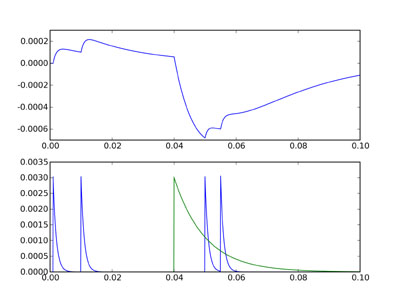
\includegraphics{2b.jpg}

The top figure shows the voltage trace, and the bottom figure shows \code{ge} in
blue and \code{gi} in green. You can see that although the inhibitory and
excitatory weights are the same, the inhibitory current is much more
powerful. This is because the effect of \code{ge} or \code{gi} on \code{V} is related to the
integral of the differential equation for those variables, and \code{gi} decays
much more slowly than \code{ge}. Thus the size of the negative deflection at
40 ms is much bigger than the excitatory ones, and even the double
excitatory spike after the inhibitory one can't cancel it out.

In the next part of this tutorial, we set up our first serious network,
with 4000 neurons, excitatory and inhibitory.


\paragraph{Exercises}
\begin{enumerate}
\item {} 
Try changing the parameters and spike times to get a feel for how it
works.

\item {} 
Try an equivalent implementation with the equation taum dV/dt = -V+ge+gi

\item {} 
Verify that the differential equation has been solved correctly.

\end{enumerate}


\paragraph{Solutions}

Solution for 2:

Simply use the line \code{C2{[}1,0{]} = -3*mV} to get the same effect.

Solution for 3:

First, set up the situation we described at the top for which we
already know the solution of the differential equations, by changing
the spike times as follows:

\begin{Verbatim}[commandchars=@\[\]]
@PYG[n][spiketimes] @PYG[o][=] @PYG[p][@PYGZlb[]]@PYG[p][(]@PYG[l+m+mi][0]@PYG[p][,]@PYG[l+m+mi][0]@PYG[o][*]@PYG[n][ms]@PYG[p][)]@PYG[p][@PYGZrb[]]
\end{Verbatim}

Now we compute what the values ought to be as follows:

\begin{Verbatim}[commandchars=@\[\]]
@PYG[n][t] @PYG[o][=] @PYG[n][Mv]@PYG[o][.]@PYG[n][times]
@PYG[n][Vpredicted] @PYG[o][=] @PYG[p][(]@PYG[n][exp]@PYG[p][(]@PYG[o][-]@PYG[n][t]@PYG[o][/]@PYG[n][taum]@PYG[p][)] @PYG[o][-] @PYG[n][exp]@PYG[p][(]@PYG[o][-]@PYG[n][t]@PYG[o][/]@PYG[n][taue]@PYG[p][)]@PYG[p][)]@PYG[o][*]@PYG[n][taue]@PYG[o][*]@PYG[p][(]@PYG[l+m+mi][3]@PYG[o][*]@PYG[n][mV]@PYG[p][)] @PYG[o][/] @PYG[p][(]@PYG[n][taum]@PYG[o][-]@PYG[n][taue]@PYG[p][)]
\end{Verbatim}

Now we can compute the difference between the predicted and actual values:

\begin{Verbatim}[commandchars=@\[\]]
@PYG[n][Vdiff] @PYG[o][=] @PYG[n+nb][abs]@PYG[p][(]@PYG[n][Vpredicted] @PYG[o][-] @PYG[n][Mv]@PYG[p][@PYGZlb[]]@PYG[l+m+mi][0]@PYG[p][@PYGZrb[]]@PYG[p][)]
\end{Verbatim}

This should be zero:

\begin{Verbatim}[commandchars=@\[\]]
@PYG[k][print] @PYG[n+nb][max]@PYG[p][(]@PYG[n][Vdiff]@PYG[p][)]
\end{Verbatim}

Sure enough, it's as close as you can expect on a computer. When I run this
it gives me the value 1.3 aV, which is 1.3 * 10\textasciicircum{}-18 volts, i.e. effectively
zero given the finite precision of the calculations involved.

\resetcurrentobjects
\hypertarget{--doc-tutorial_2c_the_cuba_network}{}

\subsubsection{Tutorial 2c: The CUBA network}

In this part of the tutorial, we set up our first serious network
that actually does something. It implements the CUBA network, Benchmark 2 from:
\begin{quote}

Simulation of networks of spiking neurons: A review of tools and strategies (2006).
Brette, Rudolph, Carnevale, Hines, Beeman, Bower, Diesmann, Goodman, Harris, Zirpe,
Natschlager, Pecevski, Ermentrout, Djurfeldt, Lansner, Rochel, Vibert, Alvarez, Muller,
Davison, El Boustani and Destexhe.
Journal of Computational Neuroscience
\end{quote}

This is a network of 4000 neurons, of which 3200 excitatory, and 800 inhibitory, with
exponential synaptic currents. The neurons are randomly connected with probability 0.02.
\begin{quote}

\begin{Verbatim}[commandchars=@\[\]]
@PYG[k+kn][from] @PYG[n+nn][brian] @PYG[k+kn][import] @PYG[o][*]

@PYG[n][taum] @PYG[o][=]  @PYG[l+m+mi][20]@PYG[o][*]@PYG[n][ms]          @PYG[c][@# membrane time constant]
@PYG[n][taue] @PYG[o][=]   @PYG[l+m+mi][5]@PYG[o][*]@PYG[n][ms]          @PYG[c][@# excitatory synaptic time constant]
@PYG[n][taui] @PYG[o][=]  @PYG[l+m+mi][10]@PYG[o][*]@PYG[n][ms]          @PYG[c][@# inhibitory synaptic time constant]
@PYG[n][Vt]   @PYG[o][=] @PYG[o][-]@PYG[l+m+mi][50]@PYG[o][*]@PYG[n][mV]          @PYG[c][@# spike threshold]
@PYG[n][Vr]   @PYG[o][=] @PYG[o][-]@PYG[l+m+mi][60]@PYG[o][*]@PYG[n][mV]          @PYG[c][@# reset value]
@PYG[n][El]   @PYG[o][=] @PYG[o][-]@PYG[l+m+mi][49]@PYG[o][*]@PYG[n][mV]          @PYG[c][@# resting potential]
@PYG[n][we]   @PYG[o][=] @PYG[p][(]@PYG[l+m+mi][60]@PYG[o][*]@PYG[l+m+mf][0.27]@PYG[o][/]@PYG[l+m+mi][10]@PYG[p][)]@PYG[o][*]@PYG[n][mV] @PYG[c][@# excitatory synaptic weight]
@PYG[n][wi]   @PYG[o][=]  @PYG[p][(]@PYG[l+m+mi][20]@PYG[o][*]@PYG[l+m+mf][4.5]@PYG[o][/]@PYG[l+m+mi][10]@PYG[p][)]@PYG[o][*]@PYG[n][mV] @PYG[c][@# inhibitory synaptic weight]

@PYG[n][eqs] @PYG[o][=] @PYG[n][Equations]@PYG[p][(]@PYG[l+s][''']
@PYG[l+s][        dV/dt  = (ge-gi-(V-El))/taum : volt]
@PYG[l+s][        dge/dt = -ge/taue            : volt]
@PYG[l+s][        dgi/dt = -gi/taui            : volt]
@PYG[l+s][        ]@PYG[l+s][''']@PYG[p][)]
\end{Verbatim}
\end{quote}

So far, this has been pretty similar to the previous part, the only
difference is we have a couple more parameters, and we've added a
resting potential \code{El} into the equation for \code{V}.

Now we make lots of neurons:
\begin{quote}

\begin{Verbatim}[commandchars=@\[\]]
@PYG[n][G] @PYG[o][=] @PYG[n][NeuronGroup]@PYG[p][(]@PYG[l+m+mi][4000]@PYG[p][,] @PYG[n][model]@PYG[o][=]@PYG[n][eqs]@PYG[p][,] @PYG[n][threshold]@PYG[o][=]@PYG[n][Vt]@PYG[p][,] @PYG[n][reset]@PYG[o][=]@PYG[n][Vr]@PYG[p][)]
\end{Verbatim}
\end{quote}

Next, we divide them into subgroups. The \hyperlink{brian.NeuronGroup.subgroup}{\code{subgroup()}} method of a
\hyperlink{brian.NeuronGroup}{\code{NeuronGroup}} returns a new \hyperlink{brian.NeuronGroup}{\code{NeuronGroup}} that can be used in
exactly the same way as its parent group. At the moment, the
subgrouping mechanism can only be used to create contiguous
groups of neurons (so you can't have a subgroup consisting
of neurons 0-100 and also 200-300 say). We designate the
first 3200 neurons as \code{Ge} and the second 800 as \code{Gi}, these
will be the excitatory and inhibitory neurons.
\begin{quote}

\begin{Verbatim}[commandchars=@\[\]]
@PYG[n][Ge] @PYG[o][=] @PYG[n][G]@PYG[o][.]@PYG[n][subgroup]@PYG[p][(]@PYG[l+m+mi][3200]@PYG[p][)] @PYG[c][@# Excitatory neurons]
@PYG[n][Gi] @PYG[o][=] @PYG[n][G]@PYG[o][.]@PYG[n][subgroup]@PYG[p][(]@PYG[l+m+mi][800]@PYG[p][)]  @PYG[c][@# Inhibitory neurons]
\end{Verbatim}
\end{quote}

Now we define the connections. As in the previous part of the
tutorial, \code{ge} is the excitatory current and \code{gi} is the inhibitory
one. \code{Ce} says that an excitatory neuron can synapse onto any
neuron in \code{G}, be it excitatory or inhibitory. Similarly for
inhibitory neurons. We also randomly connect \code{Ge} and \code{Gi} to the whole of \code{G} with
probability 0.02 and the weights given in the list of
parameters at the top.
\begin{quote}

\begin{Verbatim}[commandchars=@\[\]]
@PYG[n][Ce]@PYG[o][=]@PYG[n][Connection]@PYG[p][(]@PYG[n][Ge]@PYG[p][,] @PYG[n][G]@PYG[p][,] @PYG[l+s][']@PYG[l+s][ge]@PYG[l+s][']@PYG[p][,] @PYG[n][sparseness]@PYG[o][=]@PYG[l+m+mf][0.02]@PYG[p][,] @PYG[n][weight]@PYG[o][=]@PYG[n][we]@PYG[p][)]
@PYG[n][Ci]@PYG[o][=]@PYG[n][Connection]@PYG[p][(]@PYG[n][Gi]@PYG[p][,] @PYG[n][G]@PYG[p][,] @PYG[l+s][']@PYG[l+s][gi]@PYG[l+s][']@PYG[p][,] @PYG[n][sparseness]@PYG[o][=]@PYG[l+m+mf][0.02]@PYG[p][,] @PYG[n][weight]@PYG[o][=]@PYG[n][wi]@PYG[p][)]
\end{Verbatim}
\end{quote}

Set up some monitors as usual. The line \code{record=0} in the \hyperlink{brian.StateMonitor}{\code{StateMonitor}}
declarations indicates that we only want to record the activity of
neuron 0. This saves time and memory.
\begin{quote}

\begin{Verbatim}[commandchars=@\[\]]
@PYG[n][M]   @PYG[o][=] @PYG[n][SpikeMonitor]@PYG[p][(]@PYG[n][G]@PYG[p][)]
@PYG[n][MV]  @PYG[o][=] @PYG[n][StateMonitor]@PYG[p][(]@PYG[n][G]@PYG[p][,] @PYG[l+s][']@PYG[l+s][V]@PYG[l+s][']@PYG[p][,] @PYG[n][record]@PYG[o][=]@PYG[l+m+mi][0]@PYG[p][)]
@PYG[n][Mge] @PYG[o][=] @PYG[n][StateMonitor]@PYG[p][(]@PYG[n][G]@PYG[p][,] @PYG[l+s][']@PYG[l+s][ge]@PYG[l+s][']@PYG[p][,] @PYG[n][record]@PYG[o][=]@PYG[l+m+mi][0]@PYG[p][)]
@PYG[n][Mgi] @PYG[o][=] @PYG[n][StateMonitor]@PYG[p][(]@PYG[n][G]@PYG[p][,] @PYG[l+s][']@PYG[l+s][gi]@PYG[l+s][']@PYG[p][,] @PYG[n][record]@PYG[o][=]@PYG[l+m+mi][0]@PYG[p][)]
\end{Verbatim}
\end{quote}

And in order to start the network off in a somewhat
more realistic state, we initialise the membrane
potentials uniformly randomly between the reset and
the threshold.
\begin{quote}

\begin{Verbatim}[commandchars=@\[\]]
@PYG[n][G]@PYG[o][.]@PYG[n][V] @PYG[o][=] @PYG[n][Vr] @PYG[o][+] @PYG[p][(]@PYG[n][Vt]@PYG[o][-]@PYG[n][Vr]@PYG[p][)] @PYG[o][*] @PYG[n][rand]@PYG[p][(]@PYG[n+nb][len]@PYG[p][(]@PYG[n][G]@PYG[p][)]@PYG[p][)]
\end{Verbatim}
\end{quote}

Now we run.
\begin{quote}

\begin{Verbatim}[commandchars=@\[\]]
@PYG[n][run]@PYG[p][(]@PYG[l+m+mi][500]@PYG[o][*]@PYG[n][ms]@PYG[p][)]
\end{Verbatim}
\end{quote}

And finally we plot the results. Just for fun, we do a rather more
complicated plot than we've been doing so far, with three subplots.
The upper one is the raster plot of the whole network, and the
lower two are the values of \code{V} (on the left) and \code{ge} and \code{gi} (on the
right) for the neuron we recorded from. See the PyLab documentation
for an explanation of the plotting functions, but note that the
\hyperlink{brian.raster_plot}{\code{raster\_plot()}} keyword \code{newfigure=False} instructs the (Brian) function
\hyperlink{brian.raster_plot}{\code{raster\_plot()}} not to create a new figure (so that it can be placed
as a subplot of a larger figure).
\begin{quote}

\begin{Verbatim}[commandchars=@\[\]]
@PYG[n][subplot]@PYG[p][(]@PYG[l+m+mi][211]@PYG[p][)]
@PYG[n][raster@_plot]@PYG[p][(]@PYG[n][M]@PYG[p][,] @PYG[n][title]@PYG[o][=]@PYG[l+s][']@PYG[l+s][The CUBA network]@PYG[l+s][']@PYG[p][,] @PYG[n][newfigure]@PYG[o][=]@PYG[n+nb+bp][False]@PYG[p][)]
@PYG[n][subplot]@PYG[p][(]@PYG[l+m+mi][223]@PYG[p][)]
@PYG[n][plot]@PYG[p][(]@PYG[n][MV]@PYG[o][.]@PYG[n][times]@PYG[o][/]@PYG[n][ms]@PYG[p][,] @PYG[n][MV]@PYG[p][@PYGZlb[]]@PYG[l+m+mi][0]@PYG[p][@PYGZrb[]]@PYG[o][/]@PYG[n][mV]@PYG[p][)]
@PYG[n][xlabel]@PYG[p][(]@PYG[l+s][']@PYG[l+s][Time (ms)]@PYG[l+s][']@PYG[p][)]
@PYG[n][ylabel]@PYG[p][(]@PYG[l+s][']@PYG[l+s][V (mV)]@PYG[l+s][']@PYG[p][)]
@PYG[n][subplot]@PYG[p][(]@PYG[l+m+mi][224]@PYG[p][)]
@PYG[n][plot]@PYG[p][(]@PYG[n][Mge]@PYG[o][.]@PYG[n][times]@PYG[o][/]@PYG[n][ms]@PYG[p][,] @PYG[n][Mge]@PYG[p][@PYGZlb[]]@PYG[l+m+mi][0]@PYG[p][@PYGZrb[]]@PYG[o][/]@PYG[n][mV]@PYG[p][)]
@PYG[n][plot]@PYG[p][(]@PYG[n][Mgi]@PYG[o][.]@PYG[n][times]@PYG[o][/]@PYG[n][ms]@PYG[p][,] @PYG[n][Mgi]@PYG[p][@PYGZlb[]]@PYG[l+m+mi][0]@PYG[p][@PYGZrb[]]@PYG[o][/]@PYG[n][mV]@PYG[p][)]
@PYG[n][xlabel]@PYG[p][(]@PYG[l+s][']@PYG[l+s][Time (ms)]@PYG[l+s][']@PYG[p][)]
@PYG[n][ylabel]@PYG[p][(]@PYG[l+s][']@PYG[l+s][ge and gi (mV)]@PYG[l+s][']@PYG[p][)]
@PYG[n][legend]@PYG[p][(]@PYG[p][(]@PYG[l+s][']@PYG[l+s][ge]@PYG[l+s][']@PYG[p][,]@PYG[l+s][']@PYG[l+s][gi]@PYG[l+s][']@PYG[p][)]@PYG[p][,] @PYG[l+s][']@PYG[l+s][upper right]@PYG[l+s][']@PYG[p][)]
@PYG[n][show]@PYG[p][(]@PYG[p][)]
\end{Verbatim}
\end{quote}

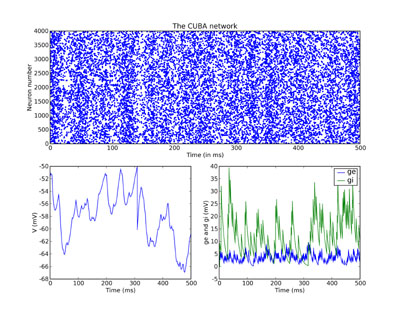
\includegraphics{2c.jpg}

\resetcurrentobjects
\hypertarget{--doc-examples}{}

\section{Examples}

These examples cover some basic topics in writing Brian scripts in Python. The
complete source code for the examples is available in the examples folder
in the extras package.


\subsection{plasticity}

\resetcurrentobjects
\hypertarget{--doc-examples-plasticity_short_term_plasticity}{}\indexii{example usage}{NeuronGroup}\indexii{example usage}{run}\indexii{example usage}{Connection}\indexii{example usage}{STP}\indexii{example usage}{stp}\indexii{example usage}{StateMonitor}

\hypertarget{index-79}{}\subsubsection{Example: short\_term\_plasticity (plasticity)}

Example with short term plasticity model
Neurons with regular inputs and depressing synapses

\begin{Verbatim}[commandchars=@\[\]]
@PYG[k+kn][from] @PYG[n+nn][brian] @PYG[k+kn][import] @PYG[o][*]

@PYG[n][tau@_e]@PYG[o][=]@PYG[l+m+mi][3]@PYG[o][*]@PYG[n][ms]
@PYG[n][taum]@PYG[o][=]@PYG[l+m+mi][10]@PYG[o][*]@PYG[n][ms]
@PYG[n][A@_SE]@PYG[o][=]@PYG[l+m+mi][250]@PYG[o][*]@PYG[n][pA]
@PYG[n][Rm]@PYG[o][=]@PYG[l+m+mi][100]@PYG[o][*]@PYG[n][Mohm]
@PYG[n][N]@PYG[o][=]@PYG[l+m+mi][10]

@PYG[n][eqs]@PYG[o][=]@PYG[l+s][''']
@PYG[l+s][dx/dt=rate : 1]
@PYG[l+s][rate : Hz]
@PYG[l+s][''']

@PYG[n+nb][input]@PYG[o][=]@PYG[n][NeuronGroup]@PYG[p][(]@PYG[n][N]@PYG[p][,]@PYG[n][model]@PYG[o][=]@PYG[n][eqs]@PYG[p][,]@PYG[n][threshold]@PYG[o][=]@PYG[l+m+mf][1.]@PYG[p][,]@PYG[n][reset]@PYG[o][=]@PYG[l+m+mi][0]@PYG[p][)]
@PYG[n+nb][input]@PYG[o][.]@PYG[n][rate]@PYG[o][=]@PYG[n][linspace]@PYG[p][(]@PYG[l+m+mi][5]@PYG[o][*]@PYG[n][Hz]@PYG[p][,]@PYG[l+m+mi][30]@PYG[o][*]@PYG[n][Hz]@PYG[p][,]@PYG[n][N]@PYG[p][)]

@PYG[n][eqs@_neuron]@PYG[o][=]@PYG[l+s][''']
@PYG[l+s][dv/dt=(Rm*i-v)/taum:volt]
@PYG[l+s][di/dt=-i/tau@_e:amp]
@PYG[l+s][''']
@PYG[n][neuron]@PYG[o][=]@PYG[n][NeuronGroup]@PYG[p][(]@PYG[n][N]@PYG[p][,]@PYG[n][model]@PYG[o][=]@PYG[n][eqs@_neuron]@PYG[p][)]

@PYG[n][C]@PYG[o][=]@PYG[n][Connection]@PYG[p][(]@PYG[n+nb][input]@PYG[p][,]@PYG[n][neuron]@PYG[p][,]@PYG[l+s][']@PYG[l+s][i]@PYG[l+s][']@PYG[p][)]
@PYG[n][C]@PYG[o][.]@PYG[n][connect@_one@_to@_one]@PYG[p][(]@PYG[n][weight]@PYG[o][=]@PYG[n][A@_SE]@PYG[p][)]
@PYG[n][stp]@PYG[o][=]@PYG[n][STP]@PYG[p][(]@PYG[n][C]@PYG[p][,]@PYG[n][taud]@PYG[o][=]@PYG[l+m+mi][1]@PYG[o][*]@PYG[n][ms]@PYG[p][,]@PYG[n][tauf]@PYG[o][=]@PYG[l+m+mi][100]@PYG[o][*]@PYG[n][ms]@PYG[p][,]@PYG[n][U]@PYG[o][=]@PYG[o][.]@PYG[l+m+mi][1]@PYG[p][)] @PYG[c][@# facilitation]
@PYG[c][@#stp=STP(C,taud=100*ms,tauf=10*ms,U=.6) @# depression]
@PYG[n][trace]@PYG[o][=]@PYG[n][StateMonitor]@PYG[p][(]@PYG[n][neuron]@PYG[p][,]@PYG[l+s][']@PYG[l+s][v]@PYG[l+s][']@PYG[p][,]@PYG[n][record]@PYG[o][=]@PYG[p][@PYGZlb[]]@PYG[l+m+mi][0]@PYG[p][,]@PYG[n][N]@PYG[o][-]@PYG[l+m+mi][1]@PYG[p][@PYGZrb[]]@PYG[p][)]

@PYG[n][run]@PYG[p][(]@PYG[l+m+mi][1000]@PYG[o][*]@PYG[n][ms]@PYG[p][)]
@PYG[n][subplot]@PYG[p][(]@PYG[l+m+mi][211]@PYG[p][)]
@PYG[n][plot]@PYG[p][(]@PYG[n][trace]@PYG[o][.]@PYG[n][times]@PYG[o][/]@PYG[n][ms]@PYG[p][,]@PYG[n][trace]@PYG[p][@PYGZlb[]]@PYG[l+m+mi][0]@PYG[p][@PYGZrb[]]@PYG[o][/]@PYG[n][mV]@PYG[p][)]
@PYG[n][title]@PYG[p][(]@PYG[l+s][']@PYG[l+s][Vm]@PYG[l+s][']@PYG[p][)]
@PYG[n][subplot]@PYG[p][(]@PYG[l+m+mi][212]@PYG[p][)]
@PYG[n][plot]@PYG[p][(]@PYG[n][trace]@PYG[o][.]@PYG[n][times]@PYG[o][/]@PYG[n][ms]@PYG[p][,]@PYG[n][trace]@PYG[p][@PYGZlb[]]@PYG[n][N]@PYG[o][-]@PYG[l+m+mi][1]@PYG[p][@PYGZrb[]]@PYG[o][/]@PYG[n][mV]@PYG[p][)]
@PYG[n][title]@PYG[p][(]@PYG[l+s][']@PYG[l+s][Vm]@PYG[l+s][']@PYG[p][)]
@PYG[n][show]@PYG[p][(]@PYG[p][)]
\end{Verbatim}

\resetcurrentobjects
\hypertarget{--doc-examples-plasticity_short_term_plasticity2}{}\indexii{example usage}{NeuronGroup}\indexii{example usage}{run}\indexii{example usage}{PopulationRateMonitor}\indexii{example usage}{raster\_plot}\indexii{example usage}{stp}\indexii{example usage}{Connection}\indexii{example usage}{SpikeMonitor}\indexii{example usage}{STP}

\hypertarget{index-80}{}\subsubsection{Example: short\_term\_plasticity2 (plasticity)}

Network (CUBA) with short-term synaptic plasticity for excitatory synapses
(Depressing at long timescales, facilitating at short timescales)

\begin{Verbatim}[commandchars=@\[\]]
@PYG[k+kn][from] @PYG[n+nn][brian] @PYG[k+kn][import] @PYG[o][*]
@PYG[k+kn][from] @PYG[n+nn][time] @PYG[k+kn][import] @PYG[n][time]

@PYG[n][eqs]@PYG[o][=]@PYG[l+s][''']
@PYG[l+s][dv/dt = (ge+gi-(v+49*mV))/(20*ms) : volt]
@PYG[l+s][dge/dt = -ge/(5*ms) : volt]
@PYG[l+s][dgi/dt = -gi/(10*ms) : volt]
@PYG[l+s][''']

@PYG[n][P]@PYG[o][=]@PYG[n][NeuronGroup]@PYG[p][(]@PYG[l+m+mi][4000]@PYG[p][,]@PYG[n][model]@PYG[o][=]@PYG[n][eqs]@PYG[p][,]@PYG[n][threshold]@PYG[o][=]@PYG[o][-]@PYG[l+m+mi][50]@PYG[o][*]@PYG[n][mV]@PYG[p][,]@PYG[n][reset]@PYG[o][=]@PYG[o][-]@PYG[l+m+mi][60]@PYG[o][*]@PYG[n][mV]@PYG[p][)]
@PYG[n][P]@PYG[o][.]@PYG[n][v]@PYG[o][=]@PYG[o][-]@PYG[l+m+mi][60]@PYG[o][*]@PYG[n][mV]@PYG[o][+]@PYG[n][rand]@PYG[p][(]@PYG[l+m+mi][4000]@PYG[p][)]@PYG[o][*]@PYG[l+m+mi][10]@PYG[o][*]@PYG[n][mV]
@PYG[n][Pe]@PYG[o][=]@PYG[n][P]@PYG[o][.]@PYG[n][subgroup]@PYG[p][(]@PYG[l+m+mi][3200]@PYG[p][)]
@PYG[n][Pi]@PYG[o][=]@PYG[n][P]@PYG[o][.]@PYG[n][subgroup]@PYG[p][(]@PYG[l+m+mi][800]@PYG[p][)]
@PYG[n][Ce]@PYG[o][=]@PYG[n][Connection]@PYG[p][(]@PYG[n][Pe]@PYG[p][,]@PYG[n][P]@PYG[p][,]@PYG[l+s][']@PYG[l+s][ge]@PYG[l+s][']@PYG[p][,]@PYG[n][weight]@PYG[o][=]@PYG[l+m+mf][1.62]@PYG[o][*]@PYG[n][mV]@PYG[p][,]@PYG[n][sparseness]@PYG[o][=]@PYG[o][.]@PYG[l+m+mo][02]@PYG[p][)]
@PYG[n][Ci]@PYG[o][=]@PYG[n][Connection]@PYG[p][(]@PYG[n][Pi]@PYG[p][,]@PYG[n][P]@PYG[p][,]@PYG[l+s][']@PYG[l+s][gi]@PYG[l+s][']@PYG[p][,]@PYG[n][weight]@PYG[o][=]@PYG[o][-]@PYG[l+m+mi][9]@PYG[o][*]@PYG[n][mV]@PYG[p][,]@PYG[n][sparseness]@PYG[o][=]@PYG[o][.]@PYG[l+m+mo][02]@PYG[p][)]
@PYG[n][stp]@PYG[o][=]@PYG[n][STP]@PYG[p][(]@PYG[n][Ce]@PYG[p][,]@PYG[n][taud]@PYG[o][=]@PYG[l+m+mi][200]@PYG[o][*]@PYG[n][ms]@PYG[p][,]@PYG[n][tauf]@PYG[o][=]@PYG[l+m+mi][20]@PYG[o][*]@PYG[n][ms]@PYG[p][,]@PYG[n][U]@PYG[o][=]@PYG[o][.]@PYG[l+m+mi][2]@PYG[p][)]
@PYG[n][M]@PYG[o][=]@PYG[n][SpikeMonitor]@PYG[p][(]@PYG[n][P]@PYG[p][)]
@PYG[n][rate]@PYG[o][=]@PYG[n][PopulationRateMonitor]@PYG[p][(]@PYG[n][P]@PYG[p][)]
@PYG[n][t1]@PYG[o][=]@PYG[n][time]@PYG[p][(]@PYG[p][)]
@PYG[n][run]@PYG[p][(]@PYG[l+m+mi][1]@PYG[o][*]@PYG[n][second]@PYG[p][)]
@PYG[n][t2]@PYG[o][=]@PYG[n][time]@PYG[p][(]@PYG[p][)]
@PYG[k][print] @PYG[l+s]["]@PYG[l+s][Simulation time:]@PYG[l+s]["]@PYG[p][,]@PYG[n][t2]@PYG[o][-]@PYG[n][t1]@PYG[p][,]@PYG[l+s]["]@PYG[l+s][s]@PYG[l+s]["]
@PYG[k][print] @PYG[n][M]@PYG[o][.]@PYG[n][nspikes]@PYG[p][,]@PYG[l+s]["]@PYG[l+s][spikes]@PYG[l+s]["]
@PYG[n][subplot]@PYG[p][(]@PYG[l+m+mi][211]@PYG[p][)]
@PYG[n][raster@_plot]@PYG[p][(]@PYG[n][M]@PYG[p][)]
@PYG[n][subplot]@PYG[p][(]@PYG[l+m+mi][212]@PYG[p][)]
@PYG[n][plot]@PYG[p][(]@PYG[n][rate]@PYG[o][.]@PYG[n][times]@PYG[o][/]@PYG[n][ms]@PYG[p][,]@PYG[n][rate]@PYG[o][.]@PYG[n][smooth@_rate]@PYG[p][(]@PYG[l+m+mi][5]@PYG[o][*]@PYG[n][ms]@PYG[p][)]@PYG[p][)]
@PYG[n][show]@PYG[p][(]@PYG[p][)]
\end{Verbatim}

\resetcurrentobjects
\hypertarget{--doc-examples-plasticity_STDP1}{}\indexii{example usage}{NeuronGroup}\indexii{example usage}{run}\indexii{example usage}{PopulationRateMonitor}\indexii{example usage}{Connection}\indexii{example usage}{STDP}\indexii{example usage}{PoissonGroup}\indexii{example usage}{stdp}

\hypertarget{index-77}{}\subsubsection{Example: STDP1 (plasticity)}

Spike-timing dependent plasticity
Adapted from Song, Miller and Abbott (2000) and Song and Abbott (2001)

This simulation takes a long time!

\begin{Verbatim}[commandchars=@\[\]]
@PYG[k+kn][from] @PYG[n+nn][brian] @PYG[k+kn][import] @PYG[o][*]
@PYG[k+kn][from] @PYG[n+nn][time] @PYG[k+kn][import] @PYG[n][time]

@PYG[n][N]@PYG[o][=]@PYG[l+m+mi][1000]
@PYG[n][taum]@PYG[o][=]@PYG[l+m+mi][10]@PYG[o][*]@PYG[n][ms]
@PYG[n][tau@_pre]@PYG[o][=]@PYG[l+m+mi][20]@PYG[o][*]@PYG[n][ms]
@PYG[n][tau@_post]@PYG[o][=]@PYG[n][tau@_pre]
@PYG[n][Ee]@PYG[o][=]@PYG[l+m+mi][0]@PYG[o][*]@PYG[n][mV]
@PYG[n][vt]@PYG[o][=]@PYG[o][-]@PYG[l+m+mi][54]@PYG[o][*]@PYG[n][mV]
@PYG[n][vr]@PYG[o][=]@PYG[o][-]@PYG[l+m+mi][60]@PYG[o][*]@PYG[n][mV]
@PYG[n][El]@PYG[o][=]@PYG[o][-]@PYG[l+m+mi][74]@PYG[o][*]@PYG[n][mV]
@PYG[n][taue]@PYG[o][=]@PYG[l+m+mi][5]@PYG[o][*]@PYG[n][ms]
@PYG[n][F]@PYG[o][=]@PYG[l+m+mi][15]@PYG[o][*]@PYG[n][Hz]
@PYG[n][gmax]@PYG[o][=]@PYG[o][.]@PYG[l+m+mo][01]
@PYG[n][dA@_pre]@PYG[o][=]@PYG[o][.]@PYG[l+m+mo][01]
@PYG[n][dA@_post]@PYG[o][=]@PYG[o][-]@PYG[n][dA@_pre]@PYG[o][*]@PYG[n][tau@_pre]@PYG[o][/]@PYG[n][tau@_post]@PYG[o][*]@PYG[l+m+mf][1.05]

@PYG[n][eqs@_neurons]@PYG[o][=]@PYG[l+s][''']
@PYG[l+s][dv/dt=(ge*(Ee-vr)+El-v)/taum : volt   @# the synaptic current is linearized]
@PYG[l+s][dge/dt=-ge/taue : 1]
@PYG[l+s][''']

@PYG[n+nb][input]@PYG[o][=]@PYG[n][PoissonGroup]@PYG[p][(]@PYG[n][N]@PYG[p][,]@PYG[n][rates]@PYG[o][=]@PYG[n][F]@PYG[p][)]
@PYG[n][neurons]@PYG[o][=]@PYG[n][NeuronGroup]@PYG[p][(]@PYG[l+m+mi][1]@PYG[p][,]@PYG[n][model]@PYG[o][=]@PYG[n][eqs@_neurons]@PYG[p][,]@PYG[n][threshold]@PYG[o][=]@PYG[n][vt]@PYG[p][,]@PYG[n][reset]@PYG[o][=]@PYG[n][vr]@PYG[p][)]
@PYG[n][synapses]@PYG[o][=]@PYG[n][Connection]@PYG[p][(]@PYG[n+nb][input]@PYG[p][,]@PYG[n][neurons]@PYG[p][,]@PYG[l+s][']@PYG[l+s][ge]@PYG[l+s][']@PYG[p][,]@PYG[n][weight]@PYG[o][=]@PYG[n][rand]@PYG[p][(]@PYG[n+nb][len]@PYG[p][(]@PYG[n+nb][input]@PYG[p][)]@PYG[p][,]@PYG[n+nb][len]@PYG[p][(]@PYG[n][neurons]@PYG[p][)]@PYG[p][)]@PYG[o][*]@PYG[n][gmax]@PYG[p][)]
@PYG[n][neurons]@PYG[o][.]@PYG[n][v]@PYG[o][=]@PYG[n][vr]

@PYG[c][@#stdp=ExponentialSTDP(synapses,tau@_pre,tau@_post,dA@_pre,dA@_post,wmax=gmax)]
@PYG[c][@#@# Explicit STDP rule]
@PYG[n][eqs@_stdp]@PYG[o][=]@PYG[l+s][''']
@PYG[l+s][dA@_pre/dt=-A@_pre/tau@_pre : 1]
@PYG[l+s][dA@_post/dt=-A@_post/tau@_post : 1]
@PYG[l+s][''']
@PYG[n][dA@_post]@PYG[o][*]@PYG[o][=]@PYG[n][gmax]
@PYG[n][dA@_pre]@PYG[o][*]@PYG[o][=]@PYG[n][gmax]
@PYG[n][stdp]@PYG[o][=]@PYG[n][STDP]@PYG[p][(]@PYG[n][synapses]@PYG[p][,]@PYG[n][eqs]@PYG[o][=]@PYG[n][eqs@_stdp]@PYG[p][,]@PYG[n][pre]@PYG[o][=]@PYG[l+s][']@PYG[l+s][A@_pre+=dA@_pre;w+=A@_post]@PYG[l+s][']@PYG[p][,]
          @PYG[n][post]@PYG[o][=]@PYG[l+s][']@PYG[l+s][A@_post+=dA@_post;w+=A@_pre]@PYG[l+s][']@PYG[p][,]@PYG[n][wmax]@PYG[o][=]@PYG[n][gmax]@PYG[p][)]

@PYG[n][rate]@PYG[o][=]@PYG[n][PopulationRateMonitor]@PYG[p][(]@PYG[n][neurons]@PYG[p][)]

@PYG[n][start@_time]@PYG[o][=]@PYG[n][time]@PYG[p][(]@PYG[p][)]
@PYG[n][run]@PYG[p][(]@PYG[l+m+mi][100]@PYG[o][*]@PYG[n][second]@PYG[p][,]@PYG[n][report]@PYG[o][=]@PYG[l+s][']@PYG[l+s][text]@PYG[l+s][']@PYG[p][)]
@PYG[k][print] @PYG[l+s]["]@PYG[l+s][Simulation time:]@PYG[l+s]["]@PYG[p][,]@PYG[n][time]@PYG[p][(]@PYG[p][)]@PYG[o][-]@PYG[n][start@_time]

@PYG[n][subplot]@PYG[p][(]@PYG[l+m+mi][311]@PYG[p][)]
@PYG[n][plot]@PYG[p][(]@PYG[n][rate]@PYG[o][.]@PYG[n][times]@PYG[o][/]@PYG[n][second]@PYG[p][,]@PYG[n][rate]@PYG[o][.]@PYG[n][smooth@_rate]@PYG[p][(]@PYG[l+m+mi][100]@PYG[o][*]@PYG[n][ms]@PYG[p][)]@PYG[p][)]
@PYG[n][subplot]@PYG[p][(]@PYG[l+m+mi][312]@PYG[p][)]
@PYG[n][plot]@PYG[p][(]@PYG[n][synapses]@PYG[o][.]@PYG[n][W]@PYG[o][.]@PYG[n][todense]@PYG[p][(]@PYG[p][)]@PYG[o][/]@PYG[n][gmax]@PYG[p][,]@PYG[l+s][']@PYG[l+s][.]@PYG[l+s][']@PYG[p][)]
@PYG[n][subplot]@PYG[p][(]@PYG[l+m+mi][313]@PYG[p][)]
@PYG[n][hist]@PYG[p][(]@PYG[n][synapses]@PYG[o][.]@PYG[n][W]@PYG[o][.]@PYG[n][todense]@PYG[p][(]@PYG[p][)]@PYG[o][/]@PYG[n][gmax]@PYG[p][,]@PYG[l+m+mi][20]@PYG[p][)]
@PYG[n][show]@PYG[p][(]@PYG[p][)]
\end{Verbatim}

\resetcurrentobjects
\hypertarget{--doc-examples-plasticity_STDP2}{}\indexii{example usage}{NeuronGroup}\indexii{example usage}{run}\indexii{example usage}{PopulationRateMonitor}\indexii{example usage}{ExponentialSTDP}\indexii{example usage}{PoissonGroup}\indexii{example usage}{Connection}\indexii{example usage}{stdp}

\hypertarget{index-78}{}\subsubsection{Example: STDP2 (plasticity)}

Spike-timing dependent plasticity
Adapted from Song, Miller and Abbott (2000), Song and Abbott (2001)
and van Rossum et al (2000).

This simulation takes a long time!

\begin{Verbatim}[commandchars=@\[\]]
@PYG[k+kn][from] @PYG[n+nn][brian] @PYG[k+kn][import] @PYG[o][*]
@PYG[k+kn][from] @PYG[n+nn][time] @PYG[k+kn][import] @PYG[n][time]

@PYG[n][N]@PYG[o][=]@PYG[l+m+mi][1000]
@PYG[n][taum]@PYG[o][=]@PYG[l+m+mi][10]@PYG[o][*]@PYG[n][ms]
@PYG[n][tau@_pre]@PYG[o][=]@PYG[l+m+mi][20]@PYG[o][*]@PYG[n][ms]
@PYG[n][tau@_post]@PYG[o][=]@PYG[n][tau@_pre]
@PYG[n][Ee]@PYG[o][=]@PYG[l+m+mi][0]@PYG[o][*]@PYG[n][mV]
@PYG[n][vt]@PYG[o][=]@PYG[o][-]@PYG[l+m+mi][54]@PYG[o][*]@PYG[n][mV]
@PYG[n][vr]@PYG[o][=]@PYG[o][-]@PYG[l+m+mi][60]@PYG[o][*]@PYG[n][mV]
@PYG[n][El]@PYG[o][=]@PYG[o][-]@PYG[l+m+mi][74]@PYG[o][*]@PYG[n][mV]
@PYG[n][taue]@PYG[o][=]@PYG[l+m+mi][5]@PYG[o][*]@PYG[n][ms]
@PYG[n][gmax]@PYG[o][=]@PYG[l+m+mf][0.01]
@PYG[n][F]@PYG[o][=]@PYG[l+m+mi][15]@PYG[o][*]@PYG[n][Hz]
@PYG[n][dA@_pre]@PYG[o][=]@PYG[o][.]@PYG[l+m+mo][01]
@PYG[n][dA@_post]@PYG[o][=]@PYG[o][-]@PYG[n][dA@_pre]@PYG[o][*]@PYG[n][tau@_pre]@PYG[o][/]@PYG[n][tau@_post]@PYG[o][*]@PYG[l+m+mf][2.5]

@PYG[n][eqs@_neurons]@PYG[o][=]@PYG[l+s][''']
@PYG[l+s][dv/dt=(ge*(Ee-vr)+El-v)/taum : volt   @# the synaptic current is linearized]
@PYG[l+s][dge/dt=-ge/taue : 1]
@PYG[l+s][''']

@PYG[n+nb][input]@PYG[o][=]@PYG[n][PoissonGroup]@PYG[p][(]@PYG[n][N]@PYG[p][,]@PYG[n][rates]@PYG[o][=]@PYG[n][F]@PYG[p][)]
@PYG[n][neurons]@PYG[o][=]@PYG[n][NeuronGroup]@PYG[p][(]@PYG[l+m+mi][1]@PYG[p][,]@PYG[n][model]@PYG[o][=]@PYG[n][eqs@_neurons]@PYG[p][,]@PYG[n][threshold]@PYG[o][=]@PYG[n][vt]@PYG[p][,]@PYG[n][reset]@PYG[o][=]@PYG[n][vr]@PYG[p][)]
@PYG[n][synapses]@PYG[o][=]@PYG[n][Connection]@PYG[p][(]@PYG[n+nb][input]@PYG[p][,]@PYG[n][neurons]@PYG[p][,]@PYG[l+s][']@PYG[l+s][ge]@PYG[l+s][']@PYG[p][,]@PYG[n][weight]@PYG[o][=]@PYG[n][rand]@PYG[p][(]@PYG[n+nb][len]@PYG[p][(]@PYG[n+nb][input]@PYG[p][)]@PYG[p][,]@PYG[n+nb][len]@PYG[p][(]@PYG[n][neurons]@PYG[p][)]@PYG[p][)]@PYG[o][*]@PYG[n][gmax]@PYG[p][,]
                    @PYG[n][structure]@PYG[o][=]@PYG[l+s][']@PYG[l+s][dense]@PYG[l+s][']@PYG[p][)]
@PYG[n][neurons]@PYG[o][.]@PYG[n][v]@PYG[o][=]@PYG[n][vr]

@PYG[n][stdp]@PYG[o][=]@PYG[n][ExponentialSTDP]@PYG[p][(]@PYG[n][synapses]@PYG[p][,]@PYG[n][tau@_pre]@PYG[p][,]@PYG[n][tau@_post]@PYG[p][,]@PYG[n][dA@_pre]@PYG[p][,]@PYG[n][dA@_post]@PYG[p][,]@PYG[n][wmax]@PYG[o][=]@PYG[n][gmax]@PYG[p][,]@PYG[n][update]@PYG[o][=]@PYG[l+s][']@PYG[l+s][mixed]@PYG[l+s][']@PYG[p][)]

@PYG[n][rate]@PYG[o][=]@PYG[n][PopulationRateMonitor]@PYG[p][(]@PYG[n][neurons]@PYG[p][)]

@PYG[n][start@_time]@PYG[o][=]@PYG[n][time]@PYG[p][(]@PYG[p][)]
@PYG[n][run]@PYG[p][(]@PYG[l+m+mi][100]@PYG[o][*]@PYG[n][second]@PYG[p][,]@PYG[n][report]@PYG[o][=]@PYG[l+s][']@PYG[l+s][text]@PYG[l+s][']@PYG[p][)]
@PYG[k][print] @PYG[l+s]["]@PYG[l+s][Simulation time:]@PYG[l+s]["]@PYG[p][,]@PYG[n][time]@PYG[p][(]@PYG[p][)]@PYG[o][-]@PYG[n][start@_time]

@PYG[n][subplot]@PYG[p][(]@PYG[l+m+mi][311]@PYG[p][)]
@PYG[n][plot]@PYG[p][(]@PYG[n][rate]@PYG[o][.]@PYG[n][times]@PYG[o][/]@PYG[n][second]@PYG[p][,]@PYG[n][rate]@PYG[o][.]@PYG[n][smooth@_rate]@PYG[p][(]@PYG[l+m+mi][100]@PYG[o][*]@PYG[n][ms]@PYG[p][)]@PYG[p][)]
@PYG[n][subplot]@PYG[p][(]@PYG[l+m+mi][312]@PYG[p][)]
@PYG[n][plot]@PYG[p][(]@PYG[n][synapses]@PYG[o][.]@PYG[n][W]@PYG[o][.]@PYG[n][todense]@PYG[p][(]@PYG[p][)]@PYG[o][/]@PYG[n][gmax]@PYG[p][,]@PYG[l+s][']@PYG[l+s][.]@PYG[l+s][']@PYG[p][)]
@PYG[n][subplot]@PYG[p][(]@PYG[l+m+mi][313]@PYG[p][)]
@PYG[n][hist]@PYG[p][(]@PYG[n][synapses]@PYG[o][.]@PYG[n][W]@PYG[o][.]@PYG[n][todense]@PYG[p][(]@PYG[p][)]@PYG[o][/]@PYG[n][gmax]@PYG[p][,]@PYG[l+m+mi][20]@PYG[p][)]
@PYG[n][show]@PYG[p][(]@PYG[p][)]
\end{Verbatim}


\subsection{multiprocessing}

\resetcurrentobjects
\hypertarget{--doc-examples-multiprocessing_multiple_runs_simple}{}

\hypertarget{example-multiprocessing-multiple-runs-simple}{}\subsubsection{Example: multiple\_runs\_simple (multiprocessing)}

Example of using Python multiprocessing module to distribute simulations over
multiple processors.

The general procedure for using multiprocessing is to define and run a network
inside a function, and then use multiprocessing.Pool.map to call the function
with multiple parameter values. Note that on Windows, any code that should only
run once should be placed inside an if \_\_name\_\_=='\_\_main\_\_' block.

\begin{Verbatim}[commandchars=@\[\]]
@PYG[k+kn][from] @PYG[n+nn][brian] @PYG[k+kn][import] @PYG[o][*]
@PYG[k+kn][import] @PYG[n+nn][multiprocessing]

@PYG[c][@# This is the function that we want to compute for various different parameters]
@PYG[k][def] @PYG[n+nf][how@_many@_spikes]@PYG[p][(]@PYG[n][excitatory@_weight]@PYG[p][)]@PYG[p][:]
    @PYG[c][@# These two lines reset the clock to 0 and clear any remaining data so that]
    @PYG[c][@# memory use doesn't build up over multiple runs.]
    @PYG[n][reinit@_default@_clock]@PYG[p][(]@PYG[p][)]
    @PYG[n][clear]@PYG[p][(]@PYG[n+nb+bp][True]@PYG[p][)]
    @PYG[n][eqs] @PYG[o][=] @PYG[l+s][''']
@PYG[l+s][    dv/dt = (ge+gi-(v+49*mV))/(20*ms) : volt]
@PYG[l+s][    dge/dt = -ge/(5*ms) : volt]
@PYG[l+s][    dgi/dt = -gi/(10*ms) : volt]
@PYG[l+s][    ]@PYG[l+s][''']
    @PYG[n][P] @PYG[o][=] @PYG[n][NeuronGroup]@PYG[p][(]@PYG[l+m+mi][4000]@PYG[p][,] @PYG[n][eqs]@PYG[p][,] @PYG[n][threshold]@PYG[o][=]@PYG[o][-]@PYG[l+m+mi][50]@PYG[o][*]@PYG[n][mV]@PYG[p][,] @PYG[n][reset]@PYG[o][=]@PYG[o][-]@PYG[l+m+mi][60]@PYG[o][*]@PYG[n][mV]@PYG[p][)]
    @PYG[n][P]@PYG[o][.]@PYG[n][v] @PYG[o][=] @PYG[o][-]@PYG[l+m+mi][60]@PYG[o][*]@PYG[n][mV]@PYG[o][+]@PYG[l+m+mi][10]@PYG[o][*]@PYG[n][mV]@PYG[o][*]@PYG[n][rand]@PYG[p][(]@PYG[n+nb][len]@PYG[p][(]@PYG[n][P]@PYG[p][)]@PYG[p][)]
    @PYG[n][Pe] @PYG[o][=] @PYG[n][P]@PYG[o][.]@PYG[n][subgroup]@PYG[p][(]@PYG[l+m+mi][3200]@PYG[p][)]
    @PYG[n][Pi] @PYG[o][=] @PYG[n][P]@PYG[o][.]@PYG[n][subgroup]@PYG[p][(]@PYG[l+m+mi][800]@PYG[p][)]
    @PYG[n][Ce] @PYG[o][=] @PYG[n][Connection]@PYG[p][(]@PYG[n][Pe]@PYG[p][,] @PYG[n][P]@PYG[p][,] @PYG[l+s][']@PYG[l+s][ge]@PYG[l+s][']@PYG[p][)]
    @PYG[n][Ci] @PYG[o][=] @PYG[n][Connection]@PYG[p][(]@PYG[n][Pi]@PYG[p][,] @PYG[n][P]@PYG[p][,] @PYG[l+s][']@PYG[l+s][gi]@PYG[l+s][']@PYG[p][)]
    @PYG[n][Ce]@PYG[o][.]@PYG[n][connect@_random]@PYG[p][(]@PYG[n][Pe]@PYG[p][,] @PYG[n][P]@PYG[p][,] @PYG[l+m+mf][0.02]@PYG[p][,] @PYG[n][weight]@PYG[o][=]@PYG[n][excitatory@_weight]@PYG[p][)]
    @PYG[n][Ci]@PYG[o][.]@PYG[n][connect@_random]@PYG[p][(]@PYG[n][Pi]@PYG[p][,] @PYG[n][P]@PYG[p][,] @PYG[l+m+mf][0.02]@PYG[p][,] @PYG[n][weight]@PYG[o][=]@PYG[o][-]@PYG[l+m+mi][9]@PYG[o][*]@PYG[n][mV]@PYG[p][)]
    @PYG[n][M] @PYG[o][=] @PYG[n][SpikeMonitor]@PYG[p][(]@PYG[n][P]@PYG[p][)]
    @PYG[n][run]@PYG[p][(]@PYG[l+m+mi][100]@PYG[o][*]@PYG[n][ms]@PYG[p][)]
    @PYG[k][return] @PYG[n][M]@PYG[o][.]@PYG[n][nspikes]

@PYG[k][if] @PYG[n][@_@_name@_@_]@PYG[o][==]@PYG[l+s][']@PYG[l+s][@_@_main@_@_]@PYG[l+s][']@PYG[p][:]
    @PYG[c][@# Note that on Windows platforms, all code that is executed rather than]
    @PYG[c][@# just defining functions and classes has to be in the if @_@_name@_@_=='@_@_main@_@_']
    @PYG[c][@# block, otherwise it will be executed by each process that starts. This]
    @PYG[c][@# isn't a problem on Linux.]
    @PYG[n][pool] @PYG[o][=] @PYG[n][multiprocessing]@PYG[o][.]@PYG[n][Pool]@PYG[p][(]@PYG[p][)] @PYG[c][@# uses num@_cpu processes by default]
    @PYG[n][weights] @PYG[o][=] @PYG[n][linspace]@PYG[p][(]@PYG[l+m+mi][0]@PYG[p][,] @PYG[l+m+mf][3.5]@PYG[p][,] @PYG[l+m+mi][100]@PYG[p][)]@PYG[o][*]@PYG[n][mV]
    @PYG[n][args] @PYG[o][=] @PYG[p][@PYGZlb[]]@PYG[n][w]@PYG[o][*]@PYG[n][volt] @PYG[k][for] @PYG[n][w] @PYG[o+ow][in] @PYG[n][weights]@PYG[p][@PYGZrb[]]
    @PYG[n][results] @PYG[o][=] @PYG[n][pool]@PYG[o][.]@PYG[n][map]@PYG[p][(]@PYG[n][how@_many@_spikes]@PYG[p][,] @PYG[n][args]@PYG[p][)] @PYG[c][@# launches multiple processes]
    @PYG[n][plot]@PYG[p][(]@PYG[n][weights]@PYG[p][,] @PYG[n][results]@PYG[p][,] @PYG[l+s][']@PYG[l+s][.]@PYG[l+s][']@PYG[p][)]
    @PYG[n][show]@PYG[p][(]@PYG[p][)]
\end{Verbatim}

\resetcurrentobjects
\hypertarget{--doc-examples-multiprocessing_multiple_runs_with_gui}{}

\hypertarget{example-multiprocessing-multiple-runs-with-gui}{}\subsubsection{Example: multiple\_runs\_with\_gui (multiprocessing)}

A complicated example of using multiprocessing for multiple runs of a simulation
with different parameters, using a GUI to monitor and control the runs.

This example features:
\begin{itemize}
\item {} 
An indefinite number of runs, with a set of parameters for each run generated
at random for each run.

\item {} 
A plot of the output of all the runs updated as soon as each run is completed.

\item {} 
A GUI showing how long each process has been running for and how long until
it completes, and with a button allowing you to terminate the runs.

\end{itemize}

A simpler example is in \code{examples/multiprocessing/multiple\_runs\_simple.py}.

\begin{Verbatim}[commandchars=@\[\]]
@PYG[c][@# We use Tk as the backend for the GUI and matplotlib so as to avoid any]
@PYG[c][@# threading conflicts]
@PYG[k+kn][import] @PYG[n+nn][matplotlib]
@PYG[n][matplotlib]@PYG[o][.]@PYG[n][use]@PYG[p][(]@PYG[l+s][']@PYG[l+s][TkAgg]@PYG[l+s][']@PYG[p][)]

@PYG[k+kn][from] @PYG[n+nn][brian] @PYG[k+kn][import] @PYG[o][*]
@PYG[k+kn][import] @PYG[n+nn][Tkinter]@PYG[o][,] @PYG[n+nn][time]@PYG[o][,] @PYG[n+nn][multiprocessing]@PYG[o][,] @PYG[n+nn][os]
@PYG[k+kn][from] @PYG[n+nn][brian.utils.progressreporting] @PYG[k+kn][import] @PYG[n][make@_text@_report]
@PYG[k+kn][from] @PYG[n+nn][Queue] @PYG[k+kn][import] @PYG[n][Empty] @PYG[k][as] @PYG[n][QueueEmpty]

@PYG[k][class] @PYG[n+nc][SimulationController]@PYG[p][(]@PYG[n][Tkinter]@PYG[o][.]@PYG[n][Tk]@PYG[p][)]@PYG[p][:]
    @PYG[l+s+sd][''']
@PYG[l+s+sd][    GUI, uses Tkinter and features a progress bar for each process, and a callback]
@PYG[l+s+sd][    function for when the terminate button is clicked.]
@PYG[l+s+sd][    ''']
    @PYG[k][def] @PYG[n+nf][@_@_init@_@_]@PYG[p][(]@PYG[n+nb+bp][self]@PYG[p][,] @PYG[n][processes]@PYG[p][,] @PYG[n][terminator]@PYG[p][,] @PYG[n][width]@PYG[o][=]@PYG[l+m+mi][600]@PYG[p][)]@PYG[p][:]
        @PYG[n][Tkinter]@PYG[o][.]@PYG[n][Tk]@PYG[o][.]@PYG[n][@_@_init@_@_]@PYG[p][(]@PYG[n+nb+bp][self]@PYG[p][,] @PYG[n+nb+bp][None]@PYG[p][)]
        @PYG[n+nb+bp][self]@PYG[o][.]@PYG[n][parent] @PYG[o][=] @PYG[n+nb+bp][None]
        @PYG[n+nb+bp][self]@PYG[o][.]@PYG[n][grid]@PYG[p][(]@PYG[p][)]
        @PYG[n][button] @PYG[o][=] @PYG[n][Tkinter]@PYG[o][.]@PYG[n][Button]@PYG[p][(]@PYG[n+nb+bp][self]@PYG[p][,] @PYG[n][text]@PYG[o][=]@PYG[l+s][']@PYG[l+s][Terminate simulation]@PYG[l+s][']@PYG[p][,]
                                @PYG[n][command]@PYG[o][=]@PYG[n][terminator]@PYG[p][)]
        @PYG[n][button]@PYG[o][.]@PYG[n][grid]@PYG[p][(]@PYG[n][column]@PYG[o][=]@PYG[l+m+mi][0]@PYG[p][,] @PYG[n][row]@PYG[o][=]@PYG[l+m+mi][0]@PYG[p][)]
        @PYG[n+nb+bp][self]@PYG[o][.]@PYG[n][pb@_width] @PYG[o][=] @PYG[n][width]
        @PYG[n+nb+bp][self]@PYG[o][.]@PYG[n][progressbars] @PYG[o][=] @PYG[p][@PYGZlb[]]@PYG[p][@PYGZrb[]]
        @PYG[k][for] @PYG[n][i] @PYG[o+ow][in] @PYG[n+nb][xrange]@PYG[p][(]@PYG[n][processes]@PYG[p][)]@PYG[p][:]
            @PYG[n][can] @PYG[o][=] @PYG[n][Tkinter]@PYG[o][.]@PYG[n][Canvas]@PYG[p][(]@PYG[n+nb+bp][self]@PYG[p][,] @PYG[n][width]@PYG[o][=]@PYG[n][width]@PYG[p][,] @PYG[n][height]@PYG[o][=]@PYG[l+m+mi][30]@PYG[p][)]
            @PYG[n][can]@PYG[o][.]@PYG[n][grid]@PYG[p][(]@PYG[n][column]@PYG[o][=]@PYG[l+m+mi][0]@PYG[p][,] @PYG[n][row]@PYG[o][=]@PYG[l+m+mi][1]@PYG[o][+]@PYG[n][i]@PYG[p][)]
            @PYG[n][can]@PYG[o][.]@PYG[n][create@_rectangle]@PYG[p][(]@PYG[l+m+mi][0]@PYG[p][,] @PYG[l+m+mi][0]@PYG[p][,] @PYG[n][width]@PYG[p][,] @PYG[l+m+mi][30]@PYG[p][,] @PYG[n][fill]@PYG[o][=]@PYG[l+s][']@PYG[l+s][@#aaaaaa]@PYG[l+s][']@PYG[p][)]
            @PYG[n][r] @PYG[o][=] @PYG[n][can]@PYG[o][.]@PYG[n][create@_rectangle]@PYG[p][(]@PYG[l+m+mi][0]@PYG[p][,] @PYG[l+m+mi][0]@PYG[p][,] @PYG[l+m+mi][0]@PYG[p][,] @PYG[l+m+mi][30]@PYG[p][,] @PYG[n][fill]@PYG[o][=]@PYG[l+s][']@PYG[l+s][@#ffaaaa]@PYG[l+s][']@PYG[p][,] @PYG[n][width]@PYG[o][=]@PYG[l+m+mi][0]@PYG[p][)]
            @PYG[n][t] @PYG[o][=] @PYG[n][can]@PYG[o][.]@PYG[n][create@_text]@PYG[p][(]@PYG[n][width]@PYG[o][/]@PYG[l+m+mi][2]@PYG[p][,] @PYG[l+m+mi][15]@PYG[p][,] @PYG[n][text]@PYG[o][=]@PYG[l+s][']@PYG[l+s][']@PYG[p][)]
            @PYG[n+nb+bp][self]@PYG[o][.]@PYG[n][progressbars]@PYG[o][.]@PYG[n][append]@PYG[p][(]@PYG[p][(]@PYG[n][can]@PYG[p][,] @PYG[n][r]@PYG[p][,] @PYG[n][t]@PYG[p][)]@PYG[p][)]
        @PYG[n+nb+bp][self]@PYG[o][.]@PYG[n][results@_text] @PYG[o][=] @PYG[n][Tkinter]@PYG[o][.]@PYG[n][Label]@PYG[p][(]@PYG[n+nb+bp][self]@PYG[p][,] @PYG[n][text]@PYG[o][=]@PYG[l+s][']@PYG[l+s][Computed 0 results, time taken: 0s]@PYG[l+s][']@PYG[p][)]
        @PYG[n+nb+bp][self]@PYG[o][.]@PYG[n][results@_text]@PYG[o][.]@PYG[n][grid]@PYG[p][(]@PYG[n][column]@PYG[o][=]@PYG[l+m+mi][0]@PYG[p][,] @PYG[n][row]@PYG[o][=]@PYG[n][processes]@PYG[o][+]@PYG[l+m+mi][1]@PYG[p][)]
        @PYG[n+nb+bp][self]@PYG[o][.]@PYG[n][title]@PYG[p][(]@PYG[l+s][']@PYG[l+s][Simulation control]@PYG[l+s][']@PYG[p][)]
    @PYG[k][def] @PYG[n+nf][update@_results]@PYG[p][(]@PYG[n+nb+bp][self]@PYG[p][,] @PYG[n][elapsed]@PYG[p][,] @PYG[n][complete]@PYG[p][)]@PYG[p][:]
        @PYG[l+s+sd][''']
@PYG[l+s+sd][        Method to update the total number of results computed and the amount of time taken.]
@PYG[l+s+sd][        ''']
        @PYG[n+nb+bp][self]@PYG[o][.]@PYG[n][results@_text]@PYG[o][.]@PYG[n][config]@PYG[p][(]@PYG[n][text]@PYG[o][=]@PYG[l+s][']@PYG[l+s][Computed ]@PYG[l+s][']@PYG[o][+]@PYG[n+nb][str]@PYG[p][(]@PYG[n][complete]@PYG[p][)]@PYG[o][+]@PYG[l+s][']@PYG[l+s][, time taken: ]@PYG[l+s][']@PYG[o][+]@PYG[n+nb][str]@PYG[p][(]@PYG[n+nb][int]@PYG[p][(]@PYG[n][elapsed]@PYG[p][)]@PYG[p][)]@PYG[o][+]@PYG[l+s][']@PYG[l+s][s]@PYG[l+s][']@PYG[p][)]
        @PYG[n+nb+bp][self]@PYG[o][.]@PYG[n][update]@PYG[p][(]@PYG[p][)]
    @PYG[k][def] @PYG[n+nf][update@_process]@PYG[p][(]@PYG[n+nb+bp][self]@PYG[p][,] @PYG[n][i]@PYG[p][,] @PYG[n][elapsed]@PYG[p][,] @PYG[n][complete]@PYG[p][,] @PYG[n][msg]@PYG[p][)]@PYG[p][:]
        @PYG[l+s+sd][''']
@PYG[l+s+sd][        Method to update the status of a given process.]
@PYG[l+s+sd][        ''']
        @PYG[n][can]@PYG[p][,] @PYG[n][r]@PYG[p][,] @PYG[n][t] @PYG[o][=] @PYG[n+nb+bp][self]@PYG[o][.]@PYG[n][progressbars]@PYG[p][@PYGZlb[]]@PYG[n][i]@PYG[p][@PYGZrb[]]
        @PYG[n][can]@PYG[o][.]@PYG[n][itemconfigure]@PYG[p][(]@PYG[n][t]@PYG[p][,] @PYG[n][text]@PYG[o][=]@PYG[l+s][']@PYG[l+s][Process ]@PYG[l+s][']@PYG[o][+]@PYG[n+nb][str]@PYG[p][(]@PYG[n][i]@PYG[p][)]@PYG[o][+]@PYG[l+s][']@PYG[l+s][: ]@PYG[l+s][']@PYG[o][+]@PYG[n][make@_text@_report]@PYG[p][(]@PYG[n][elapsed]@PYG[p][,] @PYG[n][complete]@PYG[p][)]@PYG[o][+]@PYG[l+s][']@PYG[l+s][: ]@PYG[l+s][']@PYG[o][+]@PYG[n][msg]@PYG[p][)]
        @PYG[n][can]@PYG[o][.]@PYG[n][coords]@PYG[p][(]@PYG[n][r]@PYG[p][,] @PYG[l+m+mi][0]@PYG[p][,] @PYG[l+m+mi][0]@PYG[p][,] @PYG[n+nb][int]@PYG[p][(]@PYG[n+nb+bp][self]@PYG[o][.]@PYG[n][pb@_width]@PYG[o][*]@PYG[n][complete]@PYG[p][)]@PYG[p][,] @PYG[l+m+mi][30]@PYG[p][)]
        @PYG[n+nb+bp][self]@PYG[o][.]@PYG[n][update]@PYG[p][(]@PYG[p][)]

@PYG[k][def] @PYG[n+nf][sim@_mainloop]@PYG[p][(]@PYG[n][pool]@PYG[p][,] @PYG[n][results]@PYG[p][,] @PYG[n][message@_queue]@PYG[p][)]@PYG[p][:]
    @PYG[l+s+sd][''']
@PYG[l+s+sd][    Monitors results of a simulation as they arrive]

@PYG[l+s+sd][    pool is the multiprocessing.Pool that the processes are running in,]
@PYG[l+s+sd][    results is the AsyncResult object returned by Pool.imap@_unordered which]
@PYG[l+s+sd][    returns simulation results asynchronously as and when they are ready,]
@PYG[l+s+sd][    and message@_queue is a multiprocessing.Queue used to communicate between]
@PYG[l+s+sd][    child processes and the server process. In this case, we use this Queue to]
@PYG[l+s+sd][    send messages about the percent complete and time elapsed for each run.]
@PYG[l+s+sd][    ''']
    @PYG[c][@# We use this to enumerate the processes, mapping their process IDs to an int]
    @PYG[c][@# in the range 0:num@_processes.]
    @PYG[n][pid@_to@_id] @PYG[o][=] @PYG[n+nb][dict]@PYG[p][(]@PYG[p][(]@PYG[n][pid]@PYG[p][,] @PYG[n][i]@PYG[p][)] @PYG[k][for] @PYG[n][i]@PYG[p][,] @PYG[n][pid] @PYG[o+ow][in] @PYG[n+nb][enumerate]@PYG[p][(]@PYG[p][@PYGZlb[]]@PYG[n][p]@PYG[o][.]@PYG[n][pid] @PYG[k][for] @PYG[n][p] @PYG[o+ow][in] @PYG[n][pool]@PYG[o][.]@PYG[n][@_pool]@PYG[p][@PYGZrb[]]@PYG[p][)]@PYG[p][)]
    @PYG[n][num@_processes] @PYG[o][=] @PYG[n+nb][len]@PYG[p][(]@PYG[n][pid@_to@_id]@PYG[p][)]
    @PYG[n][start] @PYG[o][=] @PYG[n][time]@PYG[o][.]@PYG[n][time]@PYG[p][(]@PYG[p][)]
    @PYG[n][stoprunningsim] @PYG[o][=] @PYG[p][@PYGZlb[]]@PYG[n+nb+bp][False]@PYG[p][@PYGZrb[]]
    @PYG[c][@# This function terminates all the pool's child processes, it is used as]
    @PYG[c][@# the callback function called when the terminate button on the GUI is clicked.]
    @PYG[k][def] @PYG[n+nf][terminate@_sim]@PYG[p][(]@PYG[p][)]@PYG[p][:]
        @PYG[n][pool]@PYG[o][.]@PYG[n][terminate]@PYG[p][(]@PYG[p][)]
        @PYG[n][stoprunningsim]@PYG[p][@PYGZlb[]]@PYG[l+m+mi][0]@PYG[p][@PYGZrb[]] @PYG[o][=] @PYG[n+nb+bp][True]
    @PYG[n][controller] @PYG[o][=] @PYG[n][SimulationController]@PYG[p][(]@PYG[n][num@_processes]@PYG[p][,] @PYG[n][terminate@_sim]@PYG[p][)]
    @PYG[k][for] @PYG[n][i] @PYG[o+ow][in] @PYG[n+nb][range]@PYG[p][(]@PYG[n][num@_processes]@PYG[p][)]@PYG[p][:]
        @PYG[n][controller]@PYG[o][.]@PYG[n][update@_process]@PYG[p][(]@PYG[n][i]@PYG[p][,] @PYG[l+m+mi][0]@PYG[p][,] @PYG[l+m+mi][0]@PYG[p][,] @PYG[l+s][']@PYG[l+s][no info yet]@PYG[l+s][']@PYG[p][)]
    @PYG[n][i] @PYG[o][=] @PYG[l+m+mi][0]
    @PYG[k][while] @PYG[n+nb+bp][True]@PYG[p][:]
        @PYG[k][try]@PYG[p][:]
            @PYG[c][@# If there is a new result (the 0.1 means wait 0.1 seconds for a]
            @PYG[c][@# result before giving up) then this try clause will execute, otherwise]
            @PYG[c][@# a TimeoutError will occur and the except clause afterwards will]
            @PYG[c][@# execute.]
            @PYG[n][weight]@PYG[p][,] @PYG[n][numspikes] @PYG[o][=] @PYG[n][results]@PYG[o][.]@PYG[n][next]@PYG[p][(]@PYG[l+m+mf][0.1]@PYG[p][)]
            @PYG[c][@# if we reach here, we have a result to plot, so we plot it and]
            @PYG[c][@# update the GUI]
            @PYG[n][plot@_result]@PYG[p][(]@PYG[n][weight]@PYG[p][,] @PYG[n][numspikes]@PYG[p][)]
            @PYG[n][i] @PYG[o][=] @PYG[n][i]@PYG[o][+]@PYG[l+m+mi][1]
            @PYG[n][controller]@PYG[o][.]@PYG[n][update@_results]@PYG[p][(]@PYG[n][time]@PYG[o][.]@PYG[n][time]@PYG[p][(]@PYG[p][)]@PYG[o][-]@PYG[n][start]@PYG[p][,] @PYG[n][i]@PYG[p][)]
        @PYG[k][except] @PYG[n][multiprocessing]@PYG[o][.]@PYG[n][TimeoutError]@PYG[p][:]
            @PYG[c][@# if we're still waiting for a new result, we can process events in]
            @PYG[c][@# the message@_queue and update the GUI if there are any.]
            @PYG[k][while] @PYG[o+ow][not] @PYG[n][message@_queue]@PYG[o][.]@PYG[n][empty]@PYG[p][(]@PYG[p][)]@PYG[p][:]
                @PYG[k][try]@PYG[p][:]
                    @PYG[c][@# messages here are of the form: (pid, elapsed, complete)]
                    @PYG[c][@# where pid is the process ID of the child process, elapsed]
                    @PYG[c][@# is the amount of time elapsed, and complete is the]
                    @PYG[c][@# fraction of the run completed. See function how@_many@_spikes]
                    @PYG[c][@# to see where these messages come from.]
                    @PYG[n][pid]@PYG[p][,] @PYG[n][elapsed]@PYG[p][,] @PYG[n][complete] @PYG[o][=] @PYG[n][message@_queue]@PYG[o][.]@PYG[n][get@_nowait]@PYG[p][(]@PYG[p][)]
                    @PYG[n][controller]@PYG[o][.]@PYG[n][update@_process]@PYG[p][(]@PYG[n][pid@_to@_id]@PYG[p][@PYGZlb[]]@PYG[n][pid]@PYG[p][@PYGZrb[]]@PYG[p][,] @PYG[n][elapsed]@PYG[p][,] @PYG[n][complete]@PYG[p][,] @PYG[l+s][']@PYG[l+s][']@PYG[p][)]
                @PYG[k][except] @PYG[n][QueueEmpty]@PYG[p][:]
                    @PYG[k][break]
            @PYG[n][controller]@PYG[o][.]@PYG[n][update]@PYG[p][(]@PYG[p][)]
            @PYG[k][if] @PYG[n][stoprunningsim]@PYG[p][@PYGZlb[]]@PYG[l+m+mi][0]@PYG[p][@PYGZrb[]]@PYG[p][:]
                @PYG[k][print] @PYG[l+s][']@PYG[l+s][Terminated simulation processes]@PYG[l+s][']
                @PYG[k][break]
    @PYG[n][controller]@PYG[o][.]@PYG[n][destroy]@PYG[p][(]@PYG[p][)]

@PYG[k][def] @PYG[n+nf][plot@_result]@PYG[p][(]@PYG[n][weight]@PYG[p][,] @PYG[n][numspikes]@PYG[p][)]@PYG[p][:]
    @PYG[n][plot]@PYG[p][(]@PYG[p][@PYGZlb[]]@PYG[n][weight]@PYG[p][@PYGZrb[]]@PYG[p][,] @PYG[p][@PYGZlb[]]@PYG[n][numspikes]@PYG[p][@PYGZrb[]]@PYG[p][,] @PYG[l+s][']@PYG[l+s][.]@PYG[l+s][']@PYG[p][,] @PYG[n][color]@PYG[o][=]@PYG[p][(]@PYG[l+m+mi][0]@PYG[p][,]@PYG[l+m+mi][0]@PYG[p][,]@PYG[l+m+mf][0.5]@PYG[p][)]@PYG[p][)]
    @PYG[n][axis]@PYG[p][(]@PYG[l+s][']@PYG[l+s][tight]@PYG[l+s][']@PYG[p][)]
    @PYG[n][draw]@PYG[p][(]@PYG[p][)] @PYG[c][@# this forces matplotlib to redraw]

@PYG[c][@# Note that how@_many@_spikes only takes one argument, which is a tuple of]
@PYG[c][@# its actual arguments. The reason for this is that Pool.imap@_unordered can only]
@PYG[c][@# pass a single argument to the function its applied to, but that argument can]
@PYG[c][@# be a tuple...]
@PYG[k][def] @PYG[n+nf][how@_many@_spikes]@PYG[p][(]@PYG[p][(]@PYG[n][excitatory@_weight]@PYG[p][,] @PYG[n][message@_queue]@PYG[p][)]@PYG[p][)]@PYG[p][:]
    @PYG[n][reinit@_default@_clock]@PYG[p][(]@PYG[p][)]
    @PYG[n][clear]@PYG[p][(]@PYG[n+nb+bp][True]@PYG[p][)]

    @PYG[n][eqs] @PYG[o][=] @PYG[l+s][''']
@PYG[l+s][    dv/dt = (ge+gi-(v+49*mV))/(20*ms) : volt]
@PYG[l+s][    dge/dt = -ge/(5*ms) : volt]
@PYG[l+s][    dgi/dt = -gi/(10*ms) : volt]
@PYG[l+s][    ]@PYG[l+s][''']
    @PYG[n][P] @PYG[o][=] @PYG[n][NeuronGroup]@PYG[p][(]@PYG[l+m+mi][4000]@PYG[p][,] @PYG[n][eqs]@PYG[p][,] @PYG[n][threshold]@PYG[o][=]@PYG[o][-]@PYG[l+m+mi][50]@PYG[o][*]@PYG[n][mV]@PYG[p][,] @PYG[n][reset]@PYG[o][=]@PYG[o][-]@PYG[l+m+mi][60]@PYG[o][*]@PYG[n][mV]@PYG[p][)]
    @PYG[n][P]@PYG[o][.]@PYG[n][v] @PYG[o][=] @PYG[o][-]@PYG[l+m+mi][60]@PYG[o][*]@PYG[n][mV]@PYG[o][+]@PYG[l+m+mi][10]@PYG[o][*]@PYG[n][mV]@PYG[o][*]@PYG[n][rand]@PYG[p][(]@PYG[n+nb][len]@PYG[p][(]@PYG[n][P]@PYG[p][)]@PYG[p][)]
    @PYG[n][Pe] @PYG[o][=] @PYG[n][P]@PYG[o][.]@PYG[n][subgroup]@PYG[p][(]@PYG[l+m+mi][3200]@PYG[p][)]
    @PYG[n][Pi] @PYG[o][=] @PYG[n][P]@PYG[o][.]@PYG[n][subgroup]@PYG[p][(]@PYG[l+m+mi][800]@PYG[p][)]
    @PYG[n][Ce] @PYG[o][=] @PYG[n][Connection]@PYG[p][(]@PYG[n][Pe]@PYG[p][,] @PYG[n][P]@PYG[p][,] @PYG[l+s][']@PYG[l+s][ge]@PYG[l+s][']@PYG[p][)]
    @PYG[n][Ci] @PYG[o][=] @PYG[n][Connection]@PYG[p][(]@PYG[n][Pi]@PYG[p][,] @PYG[n][P]@PYG[p][,] @PYG[l+s][']@PYG[l+s][gi]@PYG[l+s][']@PYG[p][)]
    @PYG[n][Ce]@PYG[o][.]@PYG[n][connect@_random]@PYG[p][(]@PYG[n][Pe]@PYG[p][,] @PYG[n][P]@PYG[p][,] @PYG[l+m+mf][0.02]@PYG[p][,] @PYG[n][weight]@PYG[o][=]@PYG[n][excitatory@_weight]@PYG[p][)]
    @PYG[n][Ci]@PYG[o][.]@PYG[n][connect@_random]@PYG[p][(]@PYG[n][Pi]@PYG[p][,] @PYG[n][P]@PYG[p][,] @PYG[l+m+mf][0.02]@PYG[p][,] @PYG[n][weight]@PYG[o][=]@PYG[o][-]@PYG[l+m+mi][9]@PYG[o][*]@PYG[n][mV]@PYG[p][)]
    @PYG[n][M] @PYG[o][=] @PYG[n][SpikeMonitor]@PYG[p][(]@PYG[n][P]@PYG[p][)]

    @PYG[c][@# This reporter function is called every second, and it sends a message to]
    @PYG[c][@# the server process updating the status of the current run.]
    @PYG[k][def] @PYG[n+nf][reporter]@PYG[p][(]@PYG[n][elapsed]@PYG[p][,] @PYG[n][complete]@PYG[p][)]@PYG[p][:]
        @PYG[n][message@_queue]@PYG[o][.]@PYG[n][put]@PYG[p][(]@PYG[p][(]@PYG[n][os]@PYG[o][.]@PYG[n][getpid]@PYG[p][(]@PYG[p][)]@PYG[p][,] @PYG[n][elapsed]@PYG[p][,] @PYG[n][complete]@PYG[p][)]@PYG[p][)]

    @PYG[n][run]@PYG[p][(]@PYG[l+m+mi][4000]@PYG[o][*]@PYG[n][ms]@PYG[p][,] @PYG[n][report]@PYG[o][=]@PYG[n][reporter]@PYG[p][,] @PYG[n][report@_period]@PYG[o][=]@PYG[l+m+mi][1]@PYG[o][*]@PYG[n][second]@PYG[p][)]

    @PYG[k][return] @PYG[p][(]@PYG[n][excitatory@_weight]@PYG[p][,] @PYG[n][M]@PYG[o][.]@PYG[n][nspikes]@PYG[p][)]


@PYG[k][if] @PYG[n][@_@_name@_@_]@PYG[o][==]@PYG[l+s][']@PYG[l+s][@_@_main@_@_]@PYG[l+s][']@PYG[p][:]
    @PYG[n][numprocesses] @PYG[o][=] @PYG[n+nb+bp][None] @PYG[c][@# number of processes to use, set to None to have one per CPU]
    @PYG[c][@# We have to use a Queue from the Manager to send messages from client]
    @PYG[c][@# processes to the server process]
    @PYG[n][manager] @PYG[o][=] @PYG[n][multiprocessing]@PYG[o][.]@PYG[n][Manager]@PYG[p][(]@PYG[p][)]
    @PYG[n][message@_queue] @PYG[o][=] @PYG[n][manager]@PYG[o][.]@PYG[n][Queue]@PYG[p][(]@PYG[p][)]
    @PYG[n][pool] @PYG[o][=] @PYG[n][multiprocessing]@PYG[o][.]@PYG[n][Pool]@PYG[p][(]@PYG[n][processes]@PYG[o][=]@PYG[n][numprocesses]@PYG[p][)]
    @PYG[c][@# This generator function repeatedly generates random sets of parameters]
    @PYG[c][@# to pass to the how@_many@_spikes function]
    @PYG[k][def] @PYG[n+nf][args]@PYG[p][(]@PYG[p][)]@PYG[p][:]
        @PYG[k][while] @PYG[n+nb+bp][True]@PYG[p][:]
            @PYG[n][weight] @PYG[o][=] @PYG[n][rand]@PYG[p][(]@PYG[p][)]@PYG[o][*]@PYG[l+m+mf][3.5]@PYG[o][*]@PYG[n][mV]
            @PYG[k][yield] @PYG[p][(]@PYG[n][weight]@PYG[p][,] @PYG[n][message@_queue]@PYG[p][)]
    @PYG[c][@# imap@_unordered returns an AsyncResult object which returns results as]
    @PYG[c][@# and when they are ready, we pass this results object which is returned]
    @PYG[c][@# immediately to the sim@_mainloop function which monitors this, updates the]
    @PYG[c][@# GUI and plots the results as they come in.]
    @PYG[n][results] @PYG[o][=] @PYG[n][pool]@PYG[o][.]@PYG[n][imap@_unordered]@PYG[p][(]@PYG[n][how@_many@_spikes]@PYG[p][,] @PYG[n][args]@PYG[p][(]@PYG[p][)]@PYG[p][)]
    @PYG[n][ion]@PYG[p][(]@PYG[p][)] @PYG[c][@# this puts matplotlib into interactive mode to plot as we go]
    @PYG[n][sim@_mainloop]@PYG[p][(]@PYG[n][pool]@PYG[p][,] @PYG[n][results]@PYG[p][,] @PYG[n][message@_queue]@PYG[p][)]
\end{Verbatim}


\subsection{modelfitting}

\resetcurrentobjects
\hypertarget{--doc-examples-modelfitting_clusterexample_manager}{}\indexii{example usage}{Equations}\indexii{example usage}{equations}

\hypertarget{index-75}{}\subsubsection{Example: clusterexample\_manager (modelfitting)}

Model fitting example using a cluster.

Fits an integrate-and-fire model to an in-vitro electrophysiological
recording over one second.

This script is the `manager' script and should be run after all the workers
have started.

\begin{Verbatim}[commandchars=@\[\]]
@PYG[k][if] @PYG[n][@_@_name@_@_] @PYG[o][==] @PYG[l+s][']@PYG[l+s][@_@_main@_@_]@PYG[l+s][']@PYG[p][:]
    @PYG[k+kn][from] @PYG[n+nn][brian] @PYG[k+kn][import] @PYG[o][*]
    @PYG[k+kn][from] @PYG[n+nn][brian.library.modelfitting] @PYG[k+kn][import] @PYG[o][*]

    @PYG[n][equations] @PYG[o][=] @PYG[n][Equations]@PYG[p][(]@PYG[l+s][''']
@PYG[l+s][        dV/dt=(R*I-V)/tau : 1]
@PYG[l+s][        I : 1]
@PYG[l+s][        R : 1]
@PYG[l+s][        tau : second]
@PYG[l+s][    ]@PYG[l+s][''']@PYG[p][)]

    @PYG[n+nb][input] @PYG[o][=] @PYG[n][loadtxt]@PYG[p][(]@PYG[l+s][']@PYG[l+s][current.txt]@PYG[l+s][']@PYG[p][)]
    @PYG[n][spikes] @PYG[o][=] @PYG[n][loadtxt]@PYG[p][(]@PYG[l+s][']@PYG[l+s][spikes.txt]@PYG[l+s][']@PYG[p][)]

    @PYG[c][@# Change this line to the hostnames or IP addresses of the workers]
    @PYG[n][machines] @PYG[o][=] @PYG[p][@PYGZlb[]]@PYG[l+s][']@PYG[l+s][localhost]@PYG[l+s][']@PYG[p][@PYGZrb[]]

    @PYG[n][params]@PYG[p][,] @PYG[n][gamma] @PYG[o][=] @PYG[n][modelfitting]@PYG[p][(]@PYG[n][model] @PYG[o][=] @PYG[n][equations]@PYG[p][,] @PYG[n][reset] @PYG[o][=] @PYG[l+m+mi][0]@PYG[p][,] @PYG[n][threshold] @PYG[o][=] @PYG[l+m+mi][1]@PYG[p][,]
                                 @PYG[n][data] @PYG[o][=] @PYG[n][spikes]@PYG[p][,]
                                 @PYG[n+nb][input] @PYG[o][=] @PYG[n+nb][input]@PYG[p][,] @PYG[n][dt] @PYG[o][=] @PYG[o][.]@PYG[l+m+mi][1]@PYG[o][*]@PYG[n][ms]@PYG[p][,]
                                 @PYG[n][particles] @PYG[o][=] @PYG[l+m+mi][1000]@PYG[p][,] @PYG[n][iterations] @PYG[o][=] @PYG[l+m+mi][3]@PYG[p][,] @PYG[n][delta] @PYG[o][=] @PYG[l+m+mi][2]@PYG[o][*]@PYG[n][ms]@PYG[p][,]
                                 @PYG[n][R] @PYG[o][=] @PYG[p][@PYGZlb[]]@PYG[l+m+mf][1.0e9]@PYG[p][,] @PYG[l+m+mf][1.0e10]@PYG[p][@PYGZrb[]]@PYG[p][,] @PYG[n][tau] @PYG[o][=] @PYG[p][@PYGZlb[]]@PYG[l+m+mi][1]@PYG[o][*]@PYG[n][ms]@PYG[p][,] @PYG[l+m+mi][50]@PYG[o][*]@PYG[n][ms]@PYG[p][@PYGZrb[]]@PYG[p][,]
                                 @PYG[n][machines]@PYG[o][=]@PYG[n][machines]@PYG[p][,] @PYG[n][use@_gpu]@PYG[o][=]@PYG[n+nb+bp][False]@PYG[p][,] @PYG[n][max@_cpu]@PYG[o][=]@PYG[l+m+mi][2]@PYG[p][)]

    @PYG[k][print] @PYG[n][params]
\end{Verbatim}

\resetcurrentobjects
\hypertarget{--doc-examples-modelfitting_clusterexample_worker}{}

\hypertarget{example-modelfitting-clusterexample-worker}{}\subsubsection{Example: clusterexample\_worker (modelfitting)}

Model fitting example using a cluster.

Fits an integrate-and-fire model to an in-vitro electrophysiological
recording over one second.

This script is the `worker' script and should be run on each worker machine
before the manager script is run.

\begin{Verbatim}[commandchars=@\[\]]
@PYG[k+kn][from] @PYG[n+nn][brian.library.modelfitting] @PYG[k+kn][import] @PYG[o][*]
@PYG[k][if] @PYG[n][@_@_name@_@_]@PYG[o][==]@PYG[l+s][']@PYG[l+s][@_@_main@_@_]@PYG[l+s][']@PYG[p][:]
    @PYG[n][modelfitting@_worker]@PYG[p][(]@PYG[n][max@_cpu]@PYG[o][=]@PYG[l+m+mi][2]@PYG[p][)]
\end{Verbatim}

\resetcurrentobjects
\hypertarget{--doc-examples-modelfitting_modelfitting}{}\indexii{example usage}{Equations}\indexii{example usage}{equations}

\hypertarget{index-76}{}\subsubsection{Example: modelfitting (modelfitting)}

Model fitting example.
Fits an integrate-and-fire model to an in-vitro electrophysiological
recording during one second.

\begin{Verbatim}[commandchars=@\[\]]
@PYG[k+kn][from] @PYG[n+nn][brian] @PYG[k+kn][import] @PYG[o][*]
@PYG[k+kn][from] @PYG[n+nn][brian.library.modelfitting] @PYG[k+kn][import] @PYG[o][*]

@PYG[k][if] @PYG[n][@_@_name@_@_] @PYG[o][==] @PYG[l+s][']@PYG[l+s][@_@_main@_@_]@PYG[l+s][']@PYG[p][:]

    @PYG[n][equations] @PYG[o][=] @PYG[n][Equations]@PYG[p][(]@PYG[l+s][''']
@PYG[l+s][        dV/dt=(R*I-V)/tau : 1]
@PYG[l+s][        I : 1]
@PYG[l+s][        R : 1]
@PYG[l+s][        tau : second]
@PYG[l+s][    ]@PYG[l+s][''']@PYG[p][)]

    @PYG[n+nb][input] @PYG[o][=] @PYG[n][loadtxt]@PYG[p][(]@PYG[l+s][']@PYG[l+s][current.txt]@PYG[l+s][']@PYG[p][)]
    @PYG[n][spikes] @PYG[o][=] @PYG[n][loadtxt]@PYG[p][(]@PYG[l+s][']@PYG[l+s][spikes.txt]@PYG[l+s][']@PYG[p][)]

    @PYG[n][params]@PYG[p][,] @PYG[n][gamma] @PYG[o][=] @PYG[n][modelfitting]@PYG[p][(]@PYG[n][model] @PYG[o][=] @PYG[n][equations]@PYG[p][,] @PYG[n][reset] @PYG[o][=] @PYG[l+m+mi][0]@PYG[p][,] @PYG[n][threshold] @PYG[o][=] @PYG[l+m+mi][1]@PYG[p][,]
                                 @PYG[n][data] @PYG[o][=] @PYG[n][spikes]@PYG[p][,]
                                 @PYG[n+nb][input] @PYG[o][=] @PYG[n+nb][input]@PYG[p][,] @PYG[n][dt] @PYG[o][=] @PYG[o][.]@PYG[l+m+mi][1]@PYG[o][*]@PYG[n][ms]@PYG[p][,]
                                 @PYG[n][particles] @PYG[o][=] @PYG[l+m+mi][1000]@PYG[p][,] @PYG[n][iterations] @PYG[o][=] @PYG[l+m+mi][3]@PYG[p][,] @PYG[n][delta] @PYG[o][=] @PYG[l+m+mi][2]@PYG[o][*]@PYG[n][ms]@PYG[p][,]
                                 @PYG[n][R] @PYG[o][=] @PYG[p][@PYGZlb[]]@PYG[l+m+mf][1.0e9]@PYG[p][,] @PYG[l+m+mf][1.0e10]@PYG[p][@PYGZrb[]]@PYG[p][,] @PYG[n][tau] @PYG[o][=] @PYG[p][@PYGZlb[]]@PYG[l+m+mi][1]@PYG[o][*]@PYG[n][ms]@PYG[p][,] @PYG[l+m+mi][50]@PYG[o][*]@PYG[n][ms]@PYG[p][@PYGZrb[]]@PYG[p][)]

    @PYG[k][print] @PYG[n][params]
\end{Verbatim}


\subsection{misc}

\resetcurrentobjects
\hypertarget{--doc-examples-misc_adaptive}{}\indexii{example usage}{NeuronGroup}\indexii{example usage}{run}\indexii{example usage}{Connection}\indexii{example usage}{PoissonGroup}\indexii{example usage}{SpikeMonitor}\indexii{example usage}{StateMonitor}

\hypertarget{index-38}{}\subsubsection{Example: adaptive (misc)}

An adaptive neuron model

\begin{Verbatim}[commandchars=@\[\]]
@PYG[k+kn][from] @PYG[n+nn][brian] @PYG[k+kn][import] @PYG[o][*]

@PYG[n][PG] @PYG[o][=] @PYG[n][PoissonGroup]@PYG[p][(]@PYG[l+m+mi][1]@PYG[p][,]@PYG[l+m+mi][500]@PYG[o][*]@PYG[n][Hz]@PYG[p][)]
@PYG[n][eqs]@PYG[o][=]@PYG[l+s][''']
@PYG[l+s][dv/dt = (-w-v)/(10*ms) : volt @# the membrane equation]
@PYG[l+s][dw/dt = -w/(30*ms) : volt @# the adaptation current]
@PYG[l+s][''']
@PYG[c][@# The adaptation variable increases with each spike]
@PYG[n][IF] @PYG[o][=] @PYG[n][NeuronGroup]@PYG[p][(]@PYG[l+m+mi][1]@PYG[p][,]@PYG[n][model]@PYG[o][=]@PYG[n][eqs]@PYG[p][,]@PYG[n][threshold]@PYG[o][=]@PYG[l+m+mi][20]@PYG[o][*]@PYG[n][mV]@PYG[p][,]
                 @PYG[n][reset]@PYG[o][=]@PYG[l+s][''']@PYG[l+s][v  = 0*mV]
@PYG[l+s][                          w += 3*mV ]@PYG[l+s][''']@PYG[p][)]

@PYG[n][C] @PYG[o][=] @PYG[n][Connection]@PYG[p][(]@PYG[n][PG]@PYG[p][,]@PYG[n][IF]@PYG[p][,]@PYG[l+s][']@PYG[l+s][v]@PYG[l+s][']@PYG[p][,]@PYG[n][weight]@PYG[o][=]@PYG[l+m+mi][3]@PYG[o][*]@PYG[n][mV]@PYG[p][)]

@PYG[n][MS] @PYG[o][=] @PYG[n][SpikeMonitor]@PYG[p][(]@PYG[n][PG]@PYG[p][,]@PYG[n+nb+bp][True]@PYG[p][)]
@PYG[n][Mv] @PYG[o][=] @PYG[n][StateMonitor]@PYG[p][(]@PYG[n][IF]@PYG[p][,]@PYG[l+s][']@PYG[l+s][v]@PYG[l+s][']@PYG[p][,]@PYG[n][record]@PYG[o][=]@PYG[n+nb+bp][True]@PYG[p][)]
@PYG[n][Mw] @PYG[o][=] @PYG[n][StateMonitor]@PYG[p][(]@PYG[n][IF]@PYG[p][,]@PYG[l+s][']@PYG[l+s][w]@PYG[l+s][']@PYG[p][,]@PYG[n][record]@PYG[o][=]@PYG[n+nb+bp][True]@PYG[p][)]

@PYG[n][run]@PYG[p][(]@PYG[l+m+mi][100]@PYG[o][*]@PYG[n][ms]@PYG[p][)]

@PYG[n][plot]@PYG[p][(]@PYG[n][Mv]@PYG[o][.]@PYG[n][times]@PYG[o][/]@PYG[n][ms]@PYG[p][,]@PYG[n][Mv]@PYG[p][@PYGZlb[]]@PYG[l+m+mi][0]@PYG[p][@PYGZrb[]]@PYG[o][/]@PYG[n][mV]@PYG[p][)]
@PYG[n][plot]@PYG[p][(]@PYG[n][Mw]@PYG[o][.]@PYG[n][times]@PYG[o][/]@PYG[n][ms]@PYG[p][,]@PYG[n][Mw]@PYG[p][@PYGZlb[]]@PYG[l+m+mi][0]@PYG[p][@PYGZrb[]]@PYG[o][/]@PYG[n][mV]@PYG[p][)]

@PYG[n][show]@PYG[p][(]@PYG[p][)]
\end{Verbatim}

\resetcurrentobjects
\hypertarget{--doc-examples-misc_adaptive_threshold}{}\indexii{example usage}{reset}\indexii{example usage}{NeuronGroup}\indexii{example usage}{run}\indexii{example usage}{Connection}\indexii{example usage}{PoissonGroup}\indexii{example usage}{StateMonitor}

\hypertarget{index-39}{}\subsubsection{Example: adaptive\_threshold (misc)}

A model with adaptive threshold (increases with each spike)

\begin{Verbatim}[commandchars=@\[\]]
@PYG[k+kn][from] @PYG[n+nn][brian] @PYG[k+kn][import] @PYG[o][*]

@PYG[n][eqs]@PYG[o][=]@PYG[l+s][''']
@PYG[l+s][dv/dt = -v/(10*ms) : volt]
@PYG[l+s][dvt/dt = (10*mV-vt)/(15*ms) : volt]
@PYG[l+s][''']

@PYG[n][reset]@PYG[o][=]@PYG[l+s][''']
@PYG[l+s][v=0*mV]
@PYG[l+s][vt+=3*mV]
@PYG[l+s][''']

@PYG[n][IF] @PYG[o][=] @PYG[n][NeuronGroup]@PYG[p][(]@PYG[l+m+mi][1]@PYG[p][,] @PYG[n][model]@PYG[o][=]@PYG[n][eqs]@PYG[p][,]@PYG[n][reset]@PYG[o][=]@PYG[n][reset]@PYG[p][,]@PYG[n][threshold]@PYG[o][=]@PYG[l+s][']@PYG[l+s][v@textgreater[]vt]@PYG[l+s][']@PYG[p][)]
@PYG[n][IF]@PYG[o][.]@PYG[n][rest]@PYG[p][(]@PYG[p][)]
@PYG[n][PG] @PYG[o][=] @PYG[n][PoissonGroup]@PYG[p][(]@PYG[l+m+mi][1]@PYG[p][,] @PYG[l+m+mi][500]@PYG[o][*]@PYG[n][Hz]@PYG[p][)]

@PYG[n][C] @PYG[o][=] @PYG[n][Connection]@PYG[p][(]@PYG[n][PG]@PYG[p][,] @PYG[n][IF]@PYG[p][,] @PYG[l+s][']@PYG[l+s][v]@PYG[l+s][']@PYG[p][,]@PYG[n][weight]@PYG[o][=]@PYG[l+m+mi][3]@PYG[o][*]@PYG[n][mV]@PYG[p][)]

@PYG[n][Mv] @PYG[o][=] @PYG[n][StateMonitor]@PYG[p][(]@PYG[n][IF]@PYG[p][,] @PYG[l+s][']@PYG[l+s][v]@PYG[l+s][']@PYG[p][,] @PYG[n][record]@PYG[o][=]@PYG[n+nb+bp][True]@PYG[p][)]
@PYG[n][Mvt] @PYG[o][=] @PYG[n][StateMonitor]@PYG[p][(]@PYG[n][IF]@PYG[p][,] @PYG[l+s][']@PYG[l+s][vt]@PYG[l+s][']@PYG[p][,] @PYG[n][record]@PYG[o][=]@PYG[n+nb+bp][True]@PYG[p][)]

@PYG[n][run]@PYG[p][(]@PYG[l+m+mi][100]@PYG[o][*]@PYG[n][ms]@PYG[p][)]

@PYG[n][plot]@PYG[p][(]@PYG[n][Mv]@PYG[o][.]@PYG[n][times]@PYG[o][/]@PYG[n][ms]@PYG[p][,] @PYG[n][Mv]@PYG[p][@PYGZlb[]]@PYG[l+m+mi][0]@PYG[p][@PYGZrb[]]@PYG[o][/]@PYG[n][mV]@PYG[p][)]
@PYG[n][plot]@PYG[p][(]@PYG[n][Mvt]@PYG[o][.]@PYG[n][times]@PYG[o][/]@PYG[n][ms]@PYG[p][,] @PYG[n][Mvt]@PYG[p][@PYGZlb[]]@PYG[l+m+mi][0]@PYG[p][@PYGZrb[]]@PYG[o][/]@PYG[n][mV]@PYG[p][)]

@PYG[n][show]@PYG[p][(]@PYG[p][)]
\end{Verbatim}

\resetcurrentobjects
\hypertarget{--doc-examples-misc_cable}{}\indexii{example usage}{NeuronGroup}\indexii{example usage}{run}\indexii{example usage}{MembraneEquation}\indexii{example usage}{Compartments}\indexii{example usage}{Current}\indexii{example usage}{StateMonitor}

\hypertarget{index-40}{}\subsubsection{Example: cable (misc)}

Dendrite with 100 compartments

\begin{Verbatim}[commandchars=@\[\]]
@PYG[k+kn][from] @PYG[n+nn][brian] @PYG[k+kn][import] @PYG[o][*]
@PYG[k+kn][from] @PYG[n+nn][brian.compartments] @PYG[k+kn][import] @PYG[o][*]
@PYG[k+kn][from] @PYG[n+nn][brian.library.ionic@_currents] @PYG[k+kn][import] @PYG[o][*]

@PYG[n][length]@PYG[o][=]@PYG[l+m+mi][1]@PYG[o][*]@PYG[n][mm]
@PYG[n][nseg]@PYG[o][=]@PYG[l+m+mi][100]
@PYG[n][dx]@PYG[o][=]@PYG[n][length]@PYG[o][/]@PYG[n][nseg]
@PYG[n][Cm]@PYG[o][=]@PYG[l+m+mi][1]@PYG[o][*]@PYG[n][uF]@PYG[o][/]@PYG[n][cm]@PYG[o][*]@PYG[o][*]@PYG[l+m+mi][2]
@PYG[n][gl]@PYG[o][=]@PYG[l+m+mf][0.02]@PYG[o][*]@PYG[n][msiemens]@PYG[o][/]@PYG[n][cm]@PYG[o][*]@PYG[o][*]@PYG[l+m+mi][2]
@PYG[n][diam]@PYG[o][=]@PYG[l+m+mi][1]@PYG[o][*]@PYG[n][um]
@PYG[n][area]@PYG[o][=]@PYG[n][pi]@PYG[o][*]@PYG[n][diam]@PYG[o][*]@PYG[n][dx]
@PYG[n][El]@PYG[o][=]@PYG[l+m+mi][0]@PYG[o][*]@PYG[n][mV]
@PYG[n][Ri]@PYG[o][=]@PYG[l+m+mi][100]@PYG[o][*]@PYG[n][ohm]@PYG[o][*]@PYG[n][cm]
@PYG[n][ra]@PYG[o][=]@PYG[n][Ri]@PYG[o][*]@PYG[l+m+mi][4]@PYG[o][/]@PYG[p][(]@PYG[n][pi]@PYG[o][*]@PYG[n][diam]@PYG[o][*]@PYG[o][*]@PYG[l+m+mi][2]@PYG[p][)]

@PYG[k][print] @PYG[l+s]["]@PYG[l+s][Time constant =]@PYG[l+s]["]@PYG[p][,]@PYG[n][Cm]@PYG[o][/]@PYG[n][gl]
@PYG[k][print] @PYG[l+s]["]@PYG[l+s][Space constant =]@PYG[l+s]["]@PYG[p][,]@PYG[o][.]@PYG[l+m+mi][5]@PYG[o][*]@PYG[p][(]@PYG[n][diam]@PYG[o][/]@PYG[p][(]@PYG[n][gl]@PYG[o][*]@PYG[n][Ri]@PYG[p][)]@PYG[p][)]@PYG[o][*]@PYG[o][*]@PYG[o][.]@PYG[l+m+mi][5]

@PYG[n][segments]@PYG[o][=]@PYG[p][{]@PYG[p][}]
@PYG[k][for] @PYG[n][i] @PYG[o+ow][in] @PYG[n+nb][range]@PYG[p][(]@PYG[n][nseg]@PYG[p][)]@PYG[p][:]
    @PYG[n][segments]@PYG[p][@PYGZlb[]]@PYG[n][i]@PYG[p][@PYGZrb[]]@PYG[o][=]@PYG[n][MembraneEquation]@PYG[p][(]@PYG[n][Cm]@PYG[o][*]@PYG[n][area]@PYG[p][)]@PYG[o][+]@PYG[n][leak@_current]@PYG[p][(]@PYG[n][gl]@PYG[o][*]@PYG[n][area]@PYG[p][,]@PYG[n][El]@PYG[p][)]

@PYG[n][segments]@PYG[p][@PYGZlb[]]@PYG[l+m+mi][0]@PYG[p][@PYGZrb[]]@PYG[o][+]@PYG[o][=]@PYG[n][Current]@PYG[p][(]@PYG[l+s][']@PYG[l+s][I:nA]@PYG[l+s][']@PYG[p][)]

@PYG[n][cable]@PYG[o][=]@PYG[n][Compartments]@PYG[p][(]@PYG[n][segments]@PYG[p][)]
@PYG[k][for] @PYG[n][i] @PYG[o+ow][in] @PYG[n+nb][range]@PYG[p][(]@PYG[n][nseg]@PYG[o][-]@PYG[l+m+mi][1]@PYG[p][)]@PYG[p][:]
    @PYG[n][cable]@PYG[o][.]@PYG[n][connect]@PYG[p][(]@PYG[n][i]@PYG[p][,]@PYG[n][i]@PYG[o][+]@PYG[l+m+mi][1]@PYG[p][,]@PYG[n][ra]@PYG[o][*]@PYG[n][dx]@PYG[p][)]

@PYG[n][neuron]@PYG[o][=]@PYG[n][NeuronGroup]@PYG[p][(]@PYG[l+m+mi][1]@PYG[p][,]@PYG[n][model]@PYG[o][=]@PYG[n][cable]@PYG[p][)]
@PYG[c][@#neuron.vm@_0=10*mV]
@PYG[n][neuron]@PYG[o][.]@PYG[n][I@_0]@PYG[o][=]@PYG[o][.]@PYG[l+m+mo][05]@PYG[o][*]@PYG[n][nA]

@PYG[n][trace]@PYG[o][=]@PYG[p][@PYGZlb[]]@PYG[p][@PYGZrb[]]
@PYG[k][for] @PYG[n][i] @PYG[o+ow][in] @PYG[n+nb][range]@PYG[p][(]@PYG[l+m+mi][10]@PYG[p][)]@PYG[p][:]
    @PYG[n][trace]@PYG[o][.]@PYG[n][append]@PYG[p][(]@PYG[n][StateMonitor]@PYG[p][(]@PYG[n][neuron]@PYG[p][,]@PYG[l+s][']@PYG[l+s][vm@_]@PYG[l+s][']@PYG[o][+]@PYG[n+nb][str]@PYG[p][(]@PYG[l+m+mi][10]@PYG[o][*]@PYG[n][i]@PYG[p][)]@PYG[p][,]@PYG[n][record]@PYG[o][=]@PYG[n+nb+bp][True]@PYG[p][)]@PYG[p][)]

@PYG[n][run]@PYG[p][(]@PYG[l+m+mi][200]@PYG[o][*]@PYG[n][ms]@PYG[p][)]

@PYG[k][for] @PYG[n][i] @PYG[o+ow][in] @PYG[n+nb][range]@PYG[p][(]@PYG[l+m+mi][10]@PYG[p][)]@PYG[p][:]
    @PYG[n][plot]@PYG[p][(]@PYG[n][trace]@PYG[p][@PYGZlb[]]@PYG[n][i]@PYG[p][@PYGZrb[]]@PYG[o][.]@PYG[n][times]@PYG[o][/]@PYG[n][ms]@PYG[p][,]@PYG[n][trace]@PYG[p][@PYGZlb[]]@PYG[n][i]@PYG[p][@PYGZrb[]]@PYG[p][@PYGZlb[]]@PYG[l+m+mi][0]@PYG[p][@PYGZrb[]]@PYG[o][/]@PYG[n][mV]@PYG[p][)]
@PYG[n][show]@PYG[p][(]@PYG[p][)]
\end{Verbatim}

\resetcurrentobjects
\hypertarget{--doc-examples-misc_COBA}{}\indexii{example usage}{PopulationSpikeCounter}\indexii{example usage}{Connection}\indexii{example usage}{Equations}\indexii{example usage}{run}\indexii{example usage}{NeuronGroup}

\hypertarget{index-32}{}\subsubsection{Example: COBA (misc)}

This is a Brian script implementing a benchmark described
in the following review paper:

Simulation of networks of spiking neurons: A review of tools and strategies (2007).
Brette, Rudolph, Carnevale, Hines, Beeman, Bower, Diesmann, Goodman, Harris, Zirpe,
Natschlager, Pecevski, Ermentrout, Djurfeldt, Lansner, Rochel, Vibert, Alvarez, Muller,
Davison, El Boustani and Destexhe.
Journal of Computational Neuroscience 23(3):349-98

Benchmark 1: random network of integrate-and-fire neurons with exponential synaptic conductances

Clock-driven implementation with Euler integration
(no spike time interpolation)


\paragraph{R. Brette - Dec 2007}

Brian is a simulator for spiking neural networks written in Python, developed by
R. Brette and D. Goodman.
\href{http://brian.di.ens.fr}{http://brian.di.ens.fr}

\begin{Verbatim}[commandchars=@\[\]]
@PYG[k+kn][from] @PYG[n+nn][brian] @PYG[k+kn][import] @PYG[o][*]
@PYG[k+kn][import] @PYG[n+nn][time]

@PYG[c][@# Time constants]
@PYG[n][taum]@PYG[o][=]@PYG[l+m+mi][20]@PYG[o][*]@PYG[n][msecond]
@PYG[n][taue]@PYG[o][=]@PYG[l+m+mi][5]@PYG[o][*]@PYG[n][msecond]
@PYG[n][taui]@PYG[o][=]@PYG[l+m+mi][10]@PYG[o][*]@PYG[n][msecond]
@PYG[c][@# Reversal potentials]
@PYG[n][Ee]@PYG[o][=]@PYG[p][(]@PYG[l+m+mf][0.]@PYG[o][+]@PYG[l+m+mf][60.]@PYG[p][)]@PYG[o][*]@PYG[n][mvolt]
@PYG[n][Ei]@PYG[o][=]@PYG[p][(]@PYG[o][-]@PYG[l+m+mf][80.]@PYG[o][+]@PYG[l+m+mf][60.]@PYG[p][)]@PYG[o][*]@PYG[n][mvolt]

@PYG[n][start@_time]@PYG[o][=]@PYG[n][time]@PYG[o][.]@PYG[n][time]@PYG[p][(]@PYG[p][)]
@PYG[n][eqs]@PYG[o][=]@PYG[n][Equations]@PYG[p][(]@PYG[l+s][''']
@PYG[l+s][dv/dt = (-v+ge*(Ee-v)+gi*(Ei-v))*(1./taum) : volt]
@PYG[l+s][dge/dt = -ge*(1./taue) : 1]
@PYG[l+s][dgi/dt = -gi*(1./taui) : 1]
@PYG[l+s][''']@PYG[p][)]
@PYG[c][@# NB 1: conductances are in units of the leak conductance]
@PYG[c][@# NB 2: multiplication is faster than division]

@PYG[n][P]@PYG[o][=]@PYG[n][NeuronGroup]@PYG[p][(]@PYG[l+m+mi][4000]@PYG[p][,]@PYG[n][model]@PYG[o][=]@PYG[n][eqs]@PYG[p][,]@PYG[n][threshold]@PYG[o][=]@PYG[l+m+mi][10]@PYG[o][*]@PYG[n][mvolt]@PYG[p][,]\
              @PYG[n][reset]@PYG[o][=]@PYG[l+m+mi][0]@PYG[o][*]@PYG[n][mvolt]@PYG[p][,]@PYG[n][refractory]@PYG[o][=]@PYG[l+m+mi][5]@PYG[o][*]@PYG[n][msecond]@PYG[p][,]
              @PYG[n][order]@PYG[o][=]@PYG[l+m+mi][1]@PYG[p][,]@PYG[n+nb][compile]@PYG[o][=]@PYG[n+nb+bp][True]@PYG[p][)]
@PYG[n][Pe]@PYG[o][=]@PYG[n][P]@PYG[o][.]@PYG[n][subgroup]@PYG[p][(]@PYG[l+m+mi][3200]@PYG[p][)]
@PYG[n][Pi]@PYG[o][=]@PYG[n][P]@PYG[o][.]@PYG[n][subgroup]@PYG[p][(]@PYG[l+m+mi][800]@PYG[p][)]
@PYG[n][we]@PYG[o][=]@PYG[l+m+mf][6.]@PYG[o][/]@PYG[l+m+mf][10.] @PYG[c][@# excitatory synaptic weight (voltage)]
@PYG[n][wi]@PYG[o][=]@PYG[l+m+mf][67.]@PYG[o][/]@PYG[l+m+mf][10.] @PYG[c][@# inhibitory synaptic weight]
@PYG[n][Ce]@PYG[o][=]@PYG[n][Connection]@PYG[p][(]@PYG[n][Pe]@PYG[p][,]@PYG[n][P]@PYG[p][,]@PYG[l+s][']@PYG[l+s][ge]@PYG[l+s][']@PYG[p][,]@PYG[n][weight]@PYG[o][=]@PYG[n][we]@PYG[p][,]@PYG[n][sparseness]@PYG[o][=]@PYG[l+m+mf][0.02]@PYG[p][)]
@PYG[n][Ci]@PYG[o][=]@PYG[n][Connection]@PYG[p][(]@PYG[n][Pi]@PYG[p][,]@PYG[n][P]@PYG[p][,]@PYG[l+s][']@PYG[l+s][gi]@PYG[l+s][']@PYG[p][,]@PYG[n][weight]@PYG[o][=]@PYG[n][wi]@PYG[p][,]@PYG[n][sparseness]@PYG[o][=]@PYG[l+m+mf][0.02]@PYG[p][)]
@PYG[c][@# Initialization]
@PYG[n][P]@PYG[o][.]@PYG[n][v]@PYG[o][=]@PYG[p][(]@PYG[n][randn]@PYG[p][(]@PYG[n+nb][len]@PYG[p][(]@PYG[n][P]@PYG[p][)]@PYG[p][)]@PYG[o][*]@PYG[l+m+mi][5]@PYG[o][-]@PYG[l+m+mi][5]@PYG[p][)]@PYG[o][*]@PYG[n][mvolt]
@PYG[n][P]@PYG[o][.]@PYG[n][ge]@PYG[o][=]@PYG[n][randn]@PYG[p][(]@PYG[n+nb][len]@PYG[p][(]@PYG[n][P]@PYG[p][)]@PYG[p][)]@PYG[o][*]@PYG[l+m+mf][1.5]@PYG[o][+]@PYG[l+m+mi][4]
@PYG[n][P]@PYG[o][.]@PYG[n][gi]@PYG[o][=]@PYG[n][randn]@PYG[p][(]@PYG[n+nb][len]@PYG[p][(]@PYG[n][P]@PYG[p][)]@PYG[p][)]@PYG[o][*]@PYG[l+m+mi][12]@PYG[o][+]@PYG[l+m+mi][20]

@PYG[c][@# Record the number of spikes]
@PYG[n][Me]@PYG[o][=]@PYG[n][PopulationSpikeCounter]@PYG[p][(]@PYG[n][Pe]@PYG[p][)]
@PYG[n][Mi]@PYG[o][=]@PYG[n][PopulationSpikeCounter]@PYG[p][(]@PYG[n][Pi]@PYG[p][)]

@PYG[k][print] @PYG[l+s]["]@PYG[l+s][Network construction time:]@PYG[l+s]["]@PYG[p][,]@PYG[n][time]@PYG[o][.]@PYG[n][time]@PYG[p][(]@PYG[p][)]@PYG[o][-]@PYG[n][start@_time]@PYG[p][,]@PYG[l+s]["]@PYG[l+s][seconds]@PYG[l+s]["]
@PYG[k][print] @PYG[l+s]["]@PYG[l+s][Simulation running...]@PYG[l+s]["]
@PYG[n][start@_time]@PYG[o][=]@PYG[n][time]@PYG[o][.]@PYG[n][time]@PYG[p][(]@PYG[p][)]

@PYG[n][run]@PYG[p][(]@PYG[l+m+mi][1]@PYG[o][*]@PYG[n][second]@PYG[p][)]
@PYG[n][duration]@PYG[o][=]@PYG[n][time]@PYG[o][.]@PYG[n][time]@PYG[p][(]@PYG[p][)]@PYG[o][-]@PYG[n][start@_time]
@PYG[k][print] @PYG[l+s]["]@PYG[l+s][Simulation time:]@PYG[l+s]["]@PYG[p][,]@PYG[n][duration]@PYG[p][,]@PYG[l+s]["]@PYG[l+s][seconds]@PYG[l+s]["]
@PYG[k][print] @PYG[n][Me]@PYG[o][.]@PYG[n][nspikes]@PYG[p][,]@PYG[l+s]["]@PYG[l+s][excitatory spikes]@PYG[l+s]["]
@PYG[k][print] @PYG[n][Mi]@PYG[o][.]@PYG[n][nspikes]@PYG[p][,]@PYG[l+s]["]@PYG[l+s][inhibitory spikes]@PYG[l+s]["]
\end{Verbatim}

\resetcurrentobjects
\hypertarget{--doc-examples-misc_COBAHH}{}\indexii{example usage}{NeuronGroup}\indexii{example usage}{run}\indexii{example usage}{PopulationSpikeCounter}\indexii{example usage}{Connection}\indexii{example usage}{EmpiricalThreshold}\indexii{example usage}{Equations}\indexii{example usage}{StateMonitor}

\hypertarget{index-33}{}\subsubsection{Example: COBAHH (misc)}

This is a Brian script implementing a benchmark described
in the following review paper:

Simulation of networks of spiking neurons: A review of tools and strategies (2007).
Brette, Rudolph, Carnevale, Hines, Beeman, Bower, Diesmann, Goodman, Harris, Zirpe,
Natschlager, Pecevski, Ermentrout, Djurfeldt, Lansner, Rochel, Vibert, Alvarez, Muller,
Davison, El Boustani and Destexhe.
Journal of Computational Neuroscience 23(3):349-98

Benchmark 3: random network of HH neurons with exponential synaptic conductances

Clock-driven implementation with exponential Euler integration
(no spike time interpolation)


\paragraph{R. Brette - Dec 2007}

Brian is a simulator for spiking neural networks written in Python, developed by
R. Brette and D. Goodman.
\href{http://brian.di.ens.fr}{http://brian.di.ens.fr}

\begin{Verbatim}[commandchars=@\[\]]
@PYG[k+kn][from] @PYG[n+nn][brian] @PYG[k+kn][import] @PYG[o][*]
@PYG[k+kn][import] @PYG[n+nn][time]

@PYG[n][use@_gpu] @PYG[o][=] @PYG[n+nb+bp][False]

@PYG[c][@# Parameters]
@PYG[n][area]@PYG[o][=]@PYG[l+m+mi][20000]@PYG[o][*]@PYG[n][umetre]@PYG[o][*]@PYG[o][*]@PYG[l+m+mi][2]
@PYG[n][Cm]@PYG[o][=]@PYG[p][(]@PYG[l+m+mi][1]@PYG[o][*]@PYG[n][ufarad]@PYG[o][*]@PYG[n][cm]@PYG[o][*]@PYG[o][*]@PYG[o][-]@PYG[l+m+mi][2]@PYG[p][)]@PYG[o][*]@PYG[n][area]
@PYG[n][gl]@PYG[o][=]@PYG[p][(]@PYG[l+m+mf][5e-5]@PYG[o][*]@PYG[n][siemens]@PYG[o][*]@PYG[n][cm]@PYG[o][*]@PYG[o][*]@PYG[o][-]@PYG[l+m+mi][2]@PYG[p][)]@PYG[o][*]@PYG[n][area]
@PYG[n][El]@PYG[o][=]@PYG[o][-]@PYG[l+m+mi][60]@PYG[o][*]@PYG[n][mV]
@PYG[n][EK]@PYG[o][=]@PYG[o][-]@PYG[l+m+mi][90]@PYG[o][*]@PYG[n][mV]
@PYG[n][ENa]@PYG[o][=]@PYG[l+m+mi][50]@PYG[o][*]@PYG[n][mV]
@PYG[n][g@_na]@PYG[o][=]@PYG[p][(]@PYG[l+m+mi][100]@PYG[o][*]@PYG[n][msiemens]@PYG[o][*]@PYG[n][cm]@PYG[o][*]@PYG[o][*]@PYG[o][-]@PYG[l+m+mi][2]@PYG[p][)]@PYG[o][*]@PYG[n][area]
@PYG[n][g@_kd]@PYG[o][=]@PYG[p][(]@PYG[l+m+mi][30]@PYG[o][*]@PYG[n][msiemens]@PYG[o][*]@PYG[n][cm]@PYG[o][*]@PYG[o][*]@PYG[o][-]@PYG[l+m+mi][2]@PYG[p][)]@PYG[o][*]@PYG[n][area]
@PYG[n][VT]@PYG[o][=]@PYG[o][-]@PYG[l+m+mi][63]@PYG[o][*]@PYG[n][mV]
@PYG[c][@# Time constants]
@PYG[n][taue]@PYG[o][=]@PYG[l+m+mi][5]@PYG[o][*]@PYG[n][ms]
@PYG[n][taui]@PYG[o][=]@PYG[l+m+mi][10]@PYG[o][*]@PYG[n][ms]
@PYG[c][@# Reversal potentials]
@PYG[n][Ee]@PYG[o][=]@PYG[l+m+mi][0]@PYG[o][*]@PYG[n][mV]
@PYG[n][Ei]@PYG[o][=]@PYG[o][-]@PYG[l+m+mi][80]@PYG[o][*]@PYG[n][mV]
@PYG[n][we]@PYG[o][=]@PYG[l+m+mi][6]@PYG[o][*]@PYG[n][nS] @PYG[c][@# excitatory synaptic weight (voltage)]
@PYG[n][wi]@PYG[o][=]@PYG[l+m+mi][67]@PYG[o][*]@PYG[n][nS] @PYG[c][@# inhibitory synaptic weight]

@PYG[n][start@_time]@PYG[o][=]@PYG[n][time]@PYG[o][.]@PYG[n][time]@PYG[p][(]@PYG[p][)]
@PYG[c][@# The model]
@PYG[n][eqs]@PYG[o][=]@PYG[n][Equations]@PYG[p][(]@PYG[l+s][''']
@PYG[l+s][dv/dt = (gl*(El-v)+ge*(Ee-v)+gi*(Ei-v)-g@_na*(m*m*m)*h*(v-ENa)-g@_kd*(n*n*n*n)*(v-EK))/Cm : volt]
@PYG[l+s][dm/dt = alpham*(1-m)-betam*m : 1]
@PYG[l+s][dn/dt = alphan*(1-n)-betan*n : 1]
@PYG[l+s][dh/dt = alphah*(1-h)-betah*h : 1]
@PYG[l+s][dge/dt = -ge*(1./taue) : siemens]
@PYG[l+s][dgi/dt = -gi*(1./taui) : siemens]
@PYG[l+s][alpham = 0.32/mV*(13*mV-v+VT)/(exp((13*mV-v+VT)/(4*mV))-1.)/ms : Hz]
@PYG[l+s][betam = 0.28/mV*(v-VT-40*mV)/(exp((v-VT-40*mV)/(5*mV))-1)/ms : Hz]
@PYG[l+s][alphah = 0.128*exp((17*mV-v+VT)/(18*mV))/ms : Hz]
@PYG[l+s][betah = 4./(1+exp((40*mV-v+VT)/(5*mV)))/ms : Hz]
@PYG[l+s][alphan = 0.032/mV*(15*mV-v+VT)/(exp((15*mV-v+VT)/(5*mV))-1.)/ms : Hz]
@PYG[l+s][betan = .5*exp((10*mV-v+VT)/(40*mV))/ms : Hz]
@PYG[l+s][''']@PYG[p][)]

@PYG[k][if] @PYG[n][use@_gpu]@PYG[p][:]
    @PYG[k+kn][from] @PYG[n+nn][brian.experimental.cuda.gpucodegen] @PYG[k+kn][import] @PYG[o][*]
    @PYG[n][defaultclock]@PYG[o][.]@PYG[n][dt] @PYG[o][=] @PYG[l+m+mf][0.05]@PYG[o][*]@PYG[n][ms]
    @PYG[n][P] @PYG[o][=] @PYG[n][GPUNeuronGroup]@PYG[p][(]@PYG[l+m+mi][4000]@PYG[p][,] @PYG[n][eqs]@PYG[p][,] @PYG[n][maxblocksize]@PYG[o][=]@PYG[l+m+mi][256]@PYG[p][,] @PYG[n][forcesync]@PYG[o][=]@PYG[n+nb+bp][True]@PYG[p][,]
                     @PYG[n][threshold]@PYG[o][=]@PYG[n][EmpiricalThreshold]@PYG[p][(]@PYG[n][threshold]@PYG[o][=]@PYG[o][-]@PYG[l+m+mi][20]@PYG[o][*]@PYG[n][mV]@PYG[p][,]@PYG[n][refractory]@PYG[o][=]@PYG[l+m+mi][3]@PYG[o][*]@PYG[n][ms]@PYG[p][)]@PYG[p][)]
@PYG[k][else]@PYG[p][:]
    @PYG[n][defaultclock]@PYG[o][.]@PYG[n][dt] @PYG[o][=] @PYG[l+m+mf][0.05]@PYG[o][*]@PYG[n][ms]
    @PYG[n][P]@PYG[o][=]@PYG[n][NeuronGroup]@PYG[p][(]@PYG[l+m+mi][4000]@PYG[p][,]@PYG[n][model]@PYG[o][=]@PYG[n][eqs]@PYG[p][,]
                  @PYG[n][threshold]@PYG[o][=]@PYG[n][EmpiricalThreshold]@PYG[p][(]@PYG[n][state]@PYG[o][=]@PYG[l+s][']@PYG[l+s][v]@PYG[l+s][']@PYG[p][,]@PYG[n][threshold]@PYG[o][=]@PYG[o][-]@PYG[l+m+mi][20]@PYG[o][*]@PYG[n][mV]@PYG[p][,]@PYG[n][refractory]@PYG[o][=]@PYG[l+m+mi][3]@PYG[o][*]@PYG[n][ms]@PYG[p][)]@PYG[p][,]
                  @PYG[c][@#freeze=True, compile=True)]
                  @PYG[n][implicit]@PYG[o][=]@PYG[n+nb+bp][True]@PYG[p][,] @PYG[n][freeze]@PYG[o][=]@PYG[n+nb+bp][True]@PYG[p][,] @PYG[n+nb][compile]@PYG[o][=]@PYG[n+nb+bp][False]@PYG[p][)]
@PYG[n][Pe]@PYG[o][=]@PYG[n][P]@PYG[o][.]@PYG[n][subgroup]@PYG[p][(]@PYG[l+m+mi][3200]@PYG[p][)]
@PYG[n][Pi]@PYG[o][=]@PYG[n][P]@PYG[o][.]@PYG[n][subgroup]@PYG[p][(]@PYG[l+m+mi][800]@PYG[p][)]
@PYG[n][Ce]@PYG[o][=]@PYG[n][Connection]@PYG[p][(]@PYG[n][Pe]@PYG[p][,]@PYG[n][P]@PYG[p][,]@PYG[l+s][']@PYG[l+s][ge]@PYG[l+s][']@PYG[p][,]@PYG[n][weight]@PYG[o][=]@PYG[n][we]@PYG[p][,]@PYG[n][sparseness]@PYG[o][=]@PYG[l+m+mf][0.02]@PYG[p][)]
@PYG[n][Ci]@PYG[o][=]@PYG[n][Connection]@PYG[p][(]@PYG[n][Pi]@PYG[p][,]@PYG[n][P]@PYG[p][,]@PYG[l+s][']@PYG[l+s][gi]@PYG[l+s][']@PYG[p][,]@PYG[n][weight]@PYG[o][=]@PYG[n][wi]@PYG[p][,]@PYG[n][sparseness]@PYG[o][=]@PYG[l+m+mf][0.02]@PYG[p][)]
@PYG[c][@# Initialization]
@PYG[n][P]@PYG[o][.]@PYG[n][v]@PYG[o][=]@PYG[n][El]@PYG[o][+]@PYG[p][(]@PYG[n][randn]@PYG[p][(]@PYG[n+nb][len]@PYG[p][(]@PYG[n][P]@PYG[p][)]@PYG[p][)]@PYG[o][*]@PYG[l+m+mi][5]@PYG[o][-]@PYG[l+m+mi][5]@PYG[p][)]@PYG[o][*]@PYG[n][mV]
@PYG[n][P]@PYG[o][.]@PYG[n][ge]@PYG[o][=]@PYG[p][(]@PYG[n][randn]@PYG[p][(]@PYG[n+nb][len]@PYG[p][(]@PYG[n][P]@PYG[p][)]@PYG[p][)]@PYG[o][*]@PYG[l+m+mf][1.5]@PYG[o][+]@PYG[l+m+mi][4]@PYG[p][)]@PYG[o][*]@PYG[l+m+mf][10.]@PYG[o][*]@PYG[n][nS]
@PYG[n][P]@PYG[o][.]@PYG[n][gi]@PYG[o][=]@PYG[p][(]@PYG[n][randn]@PYG[p][(]@PYG[n+nb][len]@PYG[p][(]@PYG[n][P]@PYG[p][)]@PYG[p][)]@PYG[o][*]@PYG[l+m+mi][12]@PYG[o][+]@PYG[l+m+mi][20]@PYG[p][)]@PYG[o][*]@PYG[l+m+mf][10.]@PYG[o][*]@PYG[n][nS]

@PYG[c][@# Record the number of spikes and a few traces]
@PYG[n][Me]@PYG[o][=]@PYG[n][PopulationSpikeCounter]@PYG[p][(]@PYG[n][Pe]@PYG[p][)]
@PYG[n][Mi]@PYG[o][=]@PYG[n][PopulationSpikeCounter]@PYG[p][(]@PYG[n][Pi]@PYG[p][)]
@PYG[n][trace]@PYG[o][=]@PYG[n][StateMonitor]@PYG[p][(]@PYG[n][P]@PYG[p][,]@PYG[l+s][']@PYG[l+s][v]@PYG[l+s][']@PYG[p][,]@PYG[n][record]@PYG[o][=]@PYG[p][@PYGZlb[]]@PYG[l+m+mi][1]@PYG[p][,]@PYG[l+m+mi][10]@PYG[p][,]@PYG[l+m+mi][100]@PYG[p][@PYGZrb[]]@PYG[p][)]

@PYG[k][print] @PYG[l+s]["]@PYG[l+s][Network construction time:]@PYG[l+s]["]@PYG[p][,]@PYG[n][time]@PYG[o][.]@PYG[n][time]@PYG[p][(]@PYG[p][)]@PYG[o][-]@PYG[n][start@_time]@PYG[p][,]@PYG[l+s]["]@PYG[l+s][seconds]@PYG[l+s]["]
@PYG[k][print] @PYG[l+s]["]@PYG[l+s][Simulation running...]@PYG[l+s]["]
@PYG[n][run]@PYG[p][(]@PYG[l+m+mi][1]@PYG[o][*]@PYG[n][msecond]@PYG[p][)]
@PYG[n][start@_time]@PYG[o][=]@PYG[n][time]@PYG[o][.]@PYG[n][time]@PYG[p][(]@PYG[p][)]

@PYG[n][run]@PYG[p][(]@PYG[l+m+mi][1000]@PYG[o][*]@PYG[n][msecond]@PYG[p][)]
@PYG[n][duration]@PYG[o][=]@PYG[n][time]@PYG[o][.]@PYG[n][time]@PYG[p][(]@PYG[p][)]@PYG[o][-]@PYG[n][start@_time]
@PYG[k][print] @PYG[l+s]["]@PYG[l+s][Simulation time:]@PYG[l+s]["]@PYG[p][,]@PYG[n][duration]@PYG[p][,]@PYG[l+s]["]@PYG[l+s][seconds]@PYG[l+s]["]
@PYG[k][print] @PYG[n][Me]@PYG[o][.]@PYG[n][nspikes]@PYG[p][,]@PYG[l+s]["]@PYG[l+s][excitatory spikes]@PYG[l+s]["]
@PYG[k][print] @PYG[n][Mi]@PYG[o][.]@PYG[n][nspikes]@PYG[p][,]@PYG[l+s]["]@PYG[l+s][inhibitory spikes]@PYG[l+s]["]

@PYG[n][plot]@PYG[p][(]@PYG[n][trace]@PYG[o][.]@PYG[n][times]@PYG[o][/]@PYG[n][ms]@PYG[p][,]@PYG[n][trace]@PYG[p][@PYGZlb[]]@PYG[l+m+mi][1]@PYG[p][@PYGZrb[]]@PYG[o][/]@PYG[n][mV]@PYG[p][)]
@PYG[n][plot]@PYG[p][(]@PYG[n][trace]@PYG[o][.]@PYG[n][times]@PYG[o][/]@PYG[n][ms]@PYG[p][,]@PYG[n][trace]@PYG[p][@PYGZlb[]]@PYG[l+m+mi][10]@PYG[p][@PYGZrb[]]@PYG[o][/]@PYG[n][mV]@PYG[p][)]
@PYG[n][plot]@PYG[p][(]@PYG[n][trace]@PYG[o][.]@PYG[n][times]@PYG[o][/]@PYG[n][ms]@PYG[p][,]@PYG[n][trace]@PYG[p][@PYGZlb[]]@PYG[l+m+mi][100]@PYG[p][@PYGZrb[]]@PYG[o][/]@PYG[n][mV]@PYG[p][)]
@PYG[n][show]@PYG[p][(]@PYG[p][)]
\end{Verbatim}

\resetcurrentobjects
\hypertarget{--doc-examples-misc_cobahh_simplified}{}\indexii{example usage}{NeuronGroup}\indexii{example usage}{run}\indexii{example usage}{Connection}\indexii{example usage}{EmpiricalThreshold}\indexii{example usage}{Equations}\indexii{example usage}{StateMonitor}

\hypertarget{index-41}{}\subsubsection{Example: cobahh\_simplified (misc)}

This is an implementation of a benchmark described
in the following review paper:

Simulation of networks of spiking neurons: A review of tools and strategies (2006).
Brette, Rudolph, Carnevale, Hines, Beeman, Bower, Diesmann, Goodman, Harris, Zirpe,
NatschlAger, Pecevski, Ermentrout, Djurfeldt, Lansner, Rochel, Vibert, Alvarez, Muller,
Davison, El Boustani and Destexhe.
Journal of Computational Neuroscience

Benchmark 3: random network of HH neurons with exponential synaptic conductances

Clock-driven implementation
(no spike time interpolation)
\begin{enumerate}
\item {} 
Brette - Dec 2007

\end{enumerate}

70s for dt=0.1 ms with exponential Euler

\begin{Verbatim}[commandchars=@\[\]]
@PYG[k+kn][from] @PYG[n+nn][brian] @PYG[k+kn][import] @PYG[o][*]

@PYG[c][@# Parameters]
@PYG[n][area]@PYG[o][=]@PYG[l+m+mi][20000]@PYG[o][*]@PYG[n][umetre]@PYG[o][*]@PYG[o][*]@PYG[l+m+mi][2]
@PYG[n][Cm]@PYG[o][=]@PYG[p][(]@PYG[l+m+mi][1]@PYG[o][*]@PYG[n][ufarad]@PYG[o][*]@PYG[n][cm]@PYG[o][*]@PYG[o][*]@PYG[o][-]@PYG[l+m+mi][2]@PYG[p][)]@PYG[o][*]@PYG[n][area]
@PYG[n][gl]@PYG[o][=]@PYG[p][(]@PYG[l+m+mf][5e-5]@PYG[o][*]@PYG[n][siemens]@PYG[o][*]@PYG[n][cm]@PYG[o][*]@PYG[o][*]@PYG[o][-]@PYG[l+m+mi][2]@PYG[p][)]@PYG[o][*]@PYG[n][area]
@PYG[n][El]@PYG[o][=]@PYG[o][-]@PYG[l+m+mi][60]@PYG[o][*]@PYG[n][mV]
@PYG[n][EK]@PYG[o][=]@PYG[o][-]@PYG[l+m+mi][90]@PYG[o][*]@PYG[n][mV]
@PYG[n][ENa]@PYG[o][=]@PYG[l+m+mi][50]@PYG[o][*]@PYG[n][mV]
@PYG[n][g@_na]@PYG[o][=]@PYG[p][(]@PYG[l+m+mi][100]@PYG[o][*]@PYG[n][msiemens]@PYG[o][*]@PYG[n][cm]@PYG[o][*]@PYG[o][*]@PYG[o][-]@PYG[l+m+mi][2]@PYG[p][)]@PYG[o][*]@PYG[n][area]
@PYG[n][g@_kd]@PYG[o][=]@PYG[p][(]@PYG[l+m+mi][30]@PYG[o][*]@PYG[n][msiemens]@PYG[o][*]@PYG[n][cm]@PYG[o][*]@PYG[o][*]@PYG[o][-]@PYG[l+m+mi][2]@PYG[p][)]@PYG[o][*]@PYG[n][area]
@PYG[n][VT]@PYG[o][=]@PYG[o][-]@PYG[l+m+mi][63]@PYG[o][*]@PYG[n][mV]
@PYG[c][@# Time constants]
@PYG[n][taue]@PYG[o][=]@PYG[l+m+mi][5]@PYG[o][*]@PYG[n][ms]
@PYG[n][taui]@PYG[o][=]@PYG[l+m+mi][10]@PYG[o][*]@PYG[n][ms]
@PYG[c][@# Reversal potentials]
@PYG[n][Ee]@PYG[o][=]@PYG[l+m+mi][0]@PYG[o][*]@PYG[n][mV]
@PYG[n][Ei]@PYG[o][=]@PYG[o][-]@PYG[l+m+mi][80]@PYG[o][*]@PYG[n][mV]
@PYG[n][we]@PYG[o][=]@PYG[l+m+mi][6]@PYG[o][*]@PYG[n][nS] @PYG[c][@# excitatory synaptic weight (voltage)]
@PYG[n][wi]@PYG[o][=]@PYG[l+m+mi][67]@PYG[o][*]@PYG[n][nS] @PYG[c][@# inhibitory synaptic weight]

@PYG[c][@# The model]
@PYG[n][eqs]@PYG[o][=]@PYG[n][Equations]@PYG[p][(]@PYG[l+s][''']
@PYG[l+s][dv/dt = (gl*(El-v)+ge*(Ee-v)+gi*(Ei-v)-]@PYG[l+s+se][\]
@PYG[l+s][    g@_na*(m*m*m)*h*(v-ENa)-]@PYG[l+s+se][\]
@PYG[l+s][    g@_kd*(n*n*n*n)*(v-EK))/Cm : volt]
@PYG[l+s][dm/dt = alpham*(1-m)-betam*m : 1]
@PYG[l+s][dn/dt = alphan*(1-n)-betan*n : 1]
@PYG[l+s][dh/dt = alphah*(1-h)-betah*h : 1]
@PYG[l+s][dge/dt = -ge*(1./taue) : siemens]
@PYG[l+s][dgi/dt = -gi*(1./taui) : siemens]
@PYG[l+s][alpham = 0.32*(mV**-1)*(13*mV-v+VT)/ ]@PYG[l+s+se][\]
@PYG[l+s][    (exp((13*mV-v+VT)/(4*mV))-1.)/ms : Hz]
@PYG[l+s][betam = 0.28*(mV**-1)*(v-VT-40*mV)/ ]@PYG[l+s+se][\]
@PYG[l+s][    (exp((v-VT-40*mV)/(5*mV))-1)/ms : Hz]
@PYG[l+s][alphah = 0.128*exp((17*mV-v+VT)/(18*mV))/ms : Hz]
@PYG[l+s][betah = 4./(1+exp((40*mV-v+VT)/(5*mV)))/ms : Hz]
@PYG[l+s][alphan = 0.032*(mV**-1)*(15*mV-v+VT)/ ]@PYG[l+s+se][\]
@PYG[l+s][    (exp((15*mV-v+VT)/(5*mV))-1.)/ms : Hz]
@PYG[l+s][betan = .5*exp((10*mV-v+VT)/(40*mV))/ms : Hz]
@PYG[l+s][''']@PYG[p][)]

@PYG[n][P]@PYG[o][=]@PYG[n][NeuronGroup]@PYG[p][(]@PYG[l+m+mi][4000]@PYG[p][,]@PYG[n][model]@PYG[o][=]@PYG[n][eqs]@PYG[p][,]
    @PYG[n][threshold]@PYG[o][=]@PYG[n][EmpiricalThreshold]@PYG[p][(]@PYG[n][threshold]@PYG[o][=]@PYG[o][-]@PYG[l+m+mi][20]@PYG[o][*]@PYG[n][mV]@PYG[p][,]
                                 @PYG[n][refractory]@PYG[o][=]@PYG[l+m+mi][3]@PYG[o][*]@PYG[n][ms]@PYG[p][)]@PYG[p][,]
    @PYG[n][implicit]@PYG[o][=]@PYG[n+nb+bp][True]@PYG[p][,]@PYG[n][freeze]@PYG[o][=]@PYG[n+nb+bp][True]@PYG[p][)]
@PYG[n][Pe]@PYG[o][=]@PYG[n][P]@PYG[o][.]@PYG[n][subgroup]@PYG[p][(]@PYG[l+m+mi][3200]@PYG[p][)]
@PYG[n][Pi]@PYG[o][=]@PYG[n][P]@PYG[o][.]@PYG[n][subgroup]@PYG[p][(]@PYG[l+m+mi][800]@PYG[p][)]
@PYG[n][Ce]@PYG[o][=]@PYG[n][Connection]@PYG[p][(]@PYG[n][Pe]@PYG[p][,]@PYG[n][P]@PYG[p][,]@PYG[l+s][']@PYG[l+s][ge]@PYG[l+s][']@PYG[p][,]@PYG[n][weight]@PYG[o][=]@PYG[n][we]@PYG[p][,]@PYG[n][sparseness]@PYG[o][=]@PYG[l+m+mf][0.02]@PYG[p][)]
@PYG[n][Ci]@PYG[o][=]@PYG[n][Connection]@PYG[p][(]@PYG[n][Pi]@PYG[p][,]@PYG[n][P]@PYG[p][,]@PYG[l+s][']@PYG[l+s][gi]@PYG[l+s][']@PYG[p][,]@PYG[n][weight]@PYG[o][=]@PYG[n][wi]@PYG[p][,]@PYG[n][sparseness]@PYG[o][=]@PYG[l+m+mf][0.02]@PYG[p][)]
@PYG[c][@# Initialization]
@PYG[n][P]@PYG[o][.]@PYG[n][v]@PYG[o][=]@PYG[n][El]@PYG[o][+]@PYG[p][(]@PYG[n][randn]@PYG[p][(]@PYG[n+nb][len]@PYG[p][(]@PYG[n][P]@PYG[p][)]@PYG[p][)]@PYG[o][*]@PYG[l+m+mi][5]@PYG[o][-]@PYG[l+m+mi][5]@PYG[p][)]@PYG[o][*]@PYG[n][mV]
@PYG[n][P]@PYG[o][.]@PYG[n][ge]@PYG[o][=]@PYG[p][(]@PYG[n][randn]@PYG[p][(]@PYG[n+nb][len]@PYG[p][(]@PYG[n][P]@PYG[p][)]@PYG[p][)]@PYG[o][*]@PYG[l+m+mf][1.5]@PYG[o][+]@PYG[l+m+mi][4]@PYG[p][)]@PYG[o][*]@PYG[l+m+mf][10.]@PYG[o][*]@PYG[n][nS]
@PYG[n][P]@PYG[o][.]@PYG[n][gi]@PYG[o][=]@PYG[p][(]@PYG[n][randn]@PYG[p][(]@PYG[n+nb][len]@PYG[p][(]@PYG[n][P]@PYG[p][)]@PYG[p][)]@PYG[o][*]@PYG[l+m+mi][12]@PYG[o][+]@PYG[l+m+mi][20]@PYG[p][)]@PYG[o][*]@PYG[l+m+mf][10.]@PYG[o][*]@PYG[n][nS]

@PYG[c][@# Record the number of spikes and a few traces]
@PYG[n][trace]@PYG[o][=]@PYG[n][StateMonitor]@PYG[p][(]@PYG[n][P]@PYG[p][,]@PYG[l+s][']@PYG[l+s][v]@PYG[l+s][']@PYG[p][,]@PYG[n][record]@PYG[o][=]@PYG[p][@PYGZlb[]]@PYG[l+m+mi][1]@PYG[p][,]@PYG[l+m+mi][10]@PYG[p][,]@PYG[l+m+mi][100]@PYG[p][@PYGZrb[]]@PYG[p][)]

@PYG[n][run]@PYG[p][(]@PYG[l+m+mi][1]@PYG[o][*]@PYG[n][second]@PYG[p][)]

@PYG[n][plot]@PYG[p][(]@PYG[n][trace]@PYG[p][@PYGZlb[]]@PYG[l+m+mi][1]@PYG[p][@PYGZrb[]]@PYG[p][)]
@PYG[n][plot]@PYG[p][(]@PYG[n][trace]@PYG[p][@PYGZlb[]]@PYG[l+m+mi][10]@PYG[p][@PYGZrb[]]@PYG[p][)]
@PYG[n][plot]@PYG[p][(]@PYG[n][trace]@PYG[p][@PYGZlb[]]@PYG[l+m+mi][100]@PYG[p][@PYGZrb[]]@PYG[p][)]
@PYG[n][show]@PYG[p][(]@PYG[p][)]
\end{Verbatim}

\resetcurrentobjects
\hypertarget{--doc-examples-misc_correlated_inputs}{}\indexii{example usage}{raster\_plot}\indexii{example usage}{SpikeMonitor}\indexii{example usage}{run}\indexii{example usage}{PopulationRateMonitor}\indexii{example usage}{StateMonitor}

\hypertarget{index-42}{}\subsubsection{Example: correlated\_inputs (misc)}

An example with correlated spike trains
From: Brette, R. (2007). Generation of correlated spike trains.

\begin{Verbatim}[commandchars=@\[\]]
@PYG[k+kn][from] @PYG[n+nn][brian] @PYG[k+kn][import] @PYG[o][*]
@PYG[k+kn][from] @PYG[n+nn][brian.correlatedspikes] @PYG[k+kn][import] @PYG[o][*]

@PYG[n+nb][input]@PYG[o][=]@PYG[n][HomogeneousCorrelatedSpikeTrains]@PYG[p][(]@PYG[l+m+mi][1000]@PYG[p][,]@PYG[n][r]@PYG[o][=]@PYG[l+m+mi][10]@PYG[o][*]@PYG[n][Hz]@PYG[p][,]@PYG[n][c]@PYG[o][=]@PYG[l+m+mf][0.1]@PYG[p][,]@PYG[n][tauc]@PYG[o][=]@PYG[l+m+mi][10]@PYG[o][*]@PYG[n][ms]@PYG[p][)]

@PYG[n][S]@PYG[o][=]@PYG[n][SpikeMonitor]@PYG[p][(]@PYG[n+nb][input]@PYG[p][)]
@PYG[n][S2]@PYG[o][=]@PYG[n][PopulationRateMonitor]@PYG[p][(]@PYG[n+nb][input]@PYG[p][)]
@PYG[n][M]@PYG[o][=]@PYG[n][StateMonitor]@PYG[p][(]@PYG[n+nb][input]@PYG[p][,]@PYG[l+s][']@PYG[l+s][rate]@PYG[l+s][']@PYG[p][,]@PYG[n][record]@PYG[o][=]@PYG[l+m+mi][0]@PYG[p][)]
@PYG[n][run]@PYG[p][(]@PYG[l+m+mi][1000]@PYG[o][*]@PYG[n][ms]@PYG[p][)]
@PYG[n][subplot]@PYG[p][(]@PYG[l+m+mi][211]@PYG[p][)]
@PYG[n][raster@_plot]@PYG[p][(]@PYG[n][S]@PYG[p][)]
@PYG[n][subplot]@PYG[p][(]@PYG[l+m+mi][212]@PYG[p][)]
@PYG[n][plot]@PYG[p][(]@PYG[n][S2]@PYG[o][.]@PYG[n][times]@PYG[o][/]@PYG[n][ms]@PYG[p][,]@PYG[n][S2]@PYG[o][.]@PYG[n][smooth@_rate]@PYG[p][(]@PYG[l+m+mi][5]@PYG[o][*]@PYG[n][ms]@PYG[p][)]@PYG[p][)]
@PYG[n][plot]@PYG[p][(]@PYG[n][M]@PYG[o][.]@PYG[n][times]@PYG[o][/]@PYG[n][ms]@PYG[p][,]@PYG[n][M]@PYG[p][@PYGZlb[]]@PYG[l+m+mi][0]@PYG[p][@PYGZrb[]]@PYG[o][/]@PYG[n][Hz]@PYG[p][)]
@PYG[n][show]@PYG[p][(]@PYG[p][)]
\end{Verbatim}

\resetcurrentobjects
\hypertarget{--doc-examples-misc_CUBA}{}\indexii{example usage}{NeuronGroup}\indexii{example usage}{run}\indexii{example usage}{PopulationRateMonitor}\indexii{example usage}{PopulationSpikeCounter}\indexii{example usage}{Connection}\indexii{example usage}{Equations}

\hypertarget{index-34}{}\subsubsection{Example: CUBA (misc)}

This is a Brian script implementing a benchmark described
in the following review paper:

Simulation of networks of spiking neurons: A review of tools and strategies (2007).
Brette, Rudolph, Carnevale, Hines, Beeman, Bower, Diesmann, Goodman, Harris, Zirpe,
Natschlager, Pecevski, Ermentrout, Djurfeldt, Lansner, Rochel, Vibert, Alvarez, Muller,
Davison, El Boustani and Destexhe.
Journal of Computational Neuroscience 23(3):349-98

Benchmark 2: random network of integrate-and-fire neurons with exponential synaptic currents

Clock-driven implementation with exact subthreshold integration
(but spike times are aligned to the grid)


\paragraph{R. Brette - Oct 2007}

Brian is a simulator for spiking neural networks written in Python, developed by
R. Brette and D. Goodman.
\href{http://brian.di.ens.fr}{http://brian.di.ens.fr}

\begin{Verbatim}[commandchars=@\[\]]
@PYG[k+kn][from] @PYG[n+nn][brian] @PYG[k+kn][import] @PYG[o][*]
@PYG[k+kn][import] @PYG[n+nn][time]

@PYG[n][start@_time]@PYG[o][=]@PYG[n][time]@PYG[o][.]@PYG[n][time]@PYG[p][(]@PYG[p][)]
@PYG[n][taum]@PYG[o][=]@PYG[l+m+mi][20]@PYG[o][*]@PYG[n][ms]
@PYG[n][taue]@PYG[o][=]@PYG[l+m+mi][5]@PYG[o][*]@PYG[n][ms]
@PYG[n][taui]@PYG[o][=]@PYG[l+m+mi][10]@PYG[o][*]@PYG[n][ms]
@PYG[n][Vt]@PYG[o][=]@PYG[o][-]@PYG[l+m+mi][50]@PYG[o][*]@PYG[n][mV]
@PYG[n][Vr]@PYG[o][=]@PYG[o][-]@PYG[l+m+mi][60]@PYG[o][*]@PYG[n][mV]
@PYG[n][El]@PYG[o][=]@PYG[o][-]@PYG[l+m+mi][49]@PYG[o][*]@PYG[n][mV]

@PYG[n][eqs]@PYG[o][=] @PYG[n][Equations]@PYG[p][(]@PYG[l+s][''']
@PYG[l+s][dv/dt  = (ge+gi-(v-El))/taum : volt]
@PYG[l+s][dge/dt = -ge/taue : volt]
@PYG[l+s][dgi/dt = -gi/taui : volt]
@PYG[l+s][''']@PYG[p][)]

@PYG[n][P]@PYG[o][=]@PYG[n][NeuronGroup]@PYG[p][(]@PYG[l+m+mi][4000]@PYG[p][,]@PYG[n][model]@PYG[o][=]@PYG[n][eqs]@PYG[p][,]@PYG[n][threshold]@PYG[o][=]@PYG[n][Vt]@PYG[p][,]@PYG[n][reset]@PYG[o][=]@PYG[n][Vr]@PYG[p][,]@PYG[n][refractory]@PYG[o][=]@PYG[l+m+mi][5]@PYG[o][*]@PYG[n][ms]@PYG[p][)]
@PYG[n][P]@PYG[o][.]@PYG[n][v]@PYG[o][=]@PYG[n][Vr]
@PYG[n][P]@PYG[o][.]@PYG[n][ge]@PYG[o][=]@PYG[l+m+mi][0]@PYG[o][*]@PYG[n][mV]
@PYG[n][P]@PYG[o][.]@PYG[n][gi]@PYG[o][=]@PYG[l+m+mi][0]@PYG[o][*]@PYG[n][mV]

@PYG[n][Pe]@PYG[o][=]@PYG[n][P]@PYG[o][.]@PYG[n][subgroup]@PYG[p][(]@PYG[l+m+mi][3200]@PYG[p][)]
@PYG[n][Pi]@PYG[o][=]@PYG[n][P]@PYG[o][.]@PYG[n][subgroup]@PYG[p][(]@PYG[l+m+mi][800]@PYG[p][)]
@PYG[n][we]@PYG[o][=]@PYG[p][(]@PYG[l+m+mi][60]@PYG[o][*]@PYG[l+m+mf][0.27]@PYG[o][/]@PYG[l+m+mi][10]@PYG[p][)]@PYG[o][*]@PYG[n][mV] @PYG[c][@# excitatory synaptic weight (voltage)]
@PYG[n][wi]@PYG[o][=]@PYG[p][(]@PYG[o][-]@PYG[l+m+mi][20]@PYG[o][*]@PYG[l+m+mf][4.5]@PYG[o][/]@PYG[l+m+mi][10]@PYG[p][)]@PYG[o][*]@PYG[n][mV] @PYG[c][@# inhibitory synaptic weight]
@PYG[n][Ce]@PYG[o][=]@PYG[n][Connection]@PYG[p][(]@PYG[n][Pe]@PYG[p][,]@PYG[n][P]@PYG[p][,]@PYG[l+s][']@PYG[l+s][ge]@PYG[l+s][']@PYG[p][,]@PYG[n][weight]@PYG[o][=]@PYG[n][we]@PYG[p][,]@PYG[n][sparseness]@PYG[o][=]@PYG[l+m+mf][0.02]@PYG[p][)]
@PYG[n][Ci]@PYG[o][=]@PYG[n][Connection]@PYG[p][(]@PYG[n][Pi]@PYG[p][,]@PYG[n][P]@PYG[p][,]@PYG[l+s][']@PYG[l+s][gi]@PYG[l+s][']@PYG[p][,]@PYG[n][weight]@PYG[o][=]@PYG[n][wi]@PYG[p][,]@PYG[n][sparseness]@PYG[o][=]@PYG[l+m+mf][0.02]@PYG[p][)]
@PYG[n][P]@PYG[o][.]@PYG[n][v]@PYG[o][=]@PYG[n][Vr]@PYG[o][+]@PYG[n][rand]@PYG[p][(]@PYG[n+nb][len]@PYG[p][(]@PYG[n][P]@PYG[p][)]@PYG[p][)]@PYG[o][*]@PYG[p][(]@PYG[n][Vt]@PYG[o][-]@PYG[n][Vr]@PYG[p][)]

@PYG[c][@# Record the number of spikes]
@PYG[n][Me]@PYG[o][=]@PYG[n][PopulationSpikeCounter]@PYG[p][(]@PYG[n][Pe]@PYG[p][)]
@PYG[n][Mi]@PYG[o][=]@PYG[n][PopulationSpikeCounter]@PYG[p][(]@PYG[n][Pi]@PYG[p][)]
@PYG[c][@# A population rate monitor]
@PYG[n][M] @PYG[o][=] @PYG[n][PopulationRateMonitor]@PYG[p][(]@PYG[n][P]@PYG[p][)]

@PYG[k][print] @PYG[l+s]["]@PYG[l+s][Network construction time:]@PYG[l+s]["]@PYG[p][,]@PYG[n][time]@PYG[o][.]@PYG[n][time]@PYG[p][(]@PYG[p][)]@PYG[o][-]@PYG[n][start@_time]@PYG[p][,]@PYG[l+s]["]@PYG[l+s][seconds]@PYG[l+s]["]
@PYG[k][print] @PYG[n+nb][len]@PYG[p][(]@PYG[n][P]@PYG[p][)]@PYG[p][,]@PYG[l+s]["]@PYG[l+s][neurons in the network]@PYG[l+s]["]
@PYG[k][print] @PYG[l+s]["]@PYG[l+s][Simulation running...]@PYG[l+s]["]
@PYG[n][run]@PYG[p][(]@PYG[l+m+mi][1]@PYG[o][*]@PYG[n][msecond]@PYG[p][)]
@PYG[n][start@_time]@PYG[o][=]@PYG[n][time]@PYG[o][.]@PYG[n][time]@PYG[p][(]@PYG[p][)]

@PYG[n][run]@PYG[p][(]@PYG[l+m+mi][1]@PYG[o][*]@PYG[n][second]@PYG[p][)]

@PYG[n][duration]@PYG[o][=]@PYG[n][time]@PYG[o][.]@PYG[n][time]@PYG[p][(]@PYG[p][)]@PYG[o][-]@PYG[n][start@_time]
@PYG[k][print] @PYG[l+s]["]@PYG[l+s][Simulation time:]@PYG[l+s]["]@PYG[p][,]@PYG[n][duration]@PYG[p][,]@PYG[l+s]["]@PYG[l+s][seconds]@PYG[l+s]["]
@PYG[k][print] @PYG[n][Me]@PYG[o][.]@PYG[n][nspikes]@PYG[p][,]@PYG[l+s]["]@PYG[l+s][excitatory spikes]@PYG[l+s]["]
@PYG[k][print] @PYG[n][Mi]@PYG[o][.]@PYG[n][nspikes]@PYG[p][,]@PYG[l+s]["]@PYG[l+s][inhibitory spikes]@PYG[l+s]["]
@PYG[n][plot]@PYG[p][(]@PYG[n][M]@PYG[o][.]@PYG[n][times]@PYG[o][/]@PYG[n][ms]@PYG[p][,]@PYG[n][M]@PYG[o][.]@PYG[n][smooth@_rate]@PYG[p][(]@PYG[l+m+mi][2]@PYG[o][*]@PYG[n][ms]@PYG[p][,]@PYG[l+s][']@PYG[l+s][gaussian]@PYG[l+s][']@PYG[p][)]@PYG[p][)]
@PYG[n][show]@PYG[p][(]@PYG[p][)]
\end{Verbatim}

\resetcurrentobjects
\hypertarget{--doc-examples-misc_current_clamp}{}\indexii{example usage}{NeuronGroup}\indexii{example usage}{Equations}\indexii{example usage}{run}\indexii{example usage}{StateMonitor}

\hypertarget{index-43}{}\subsubsection{Example: current\_clamp (misc)}

An example of single-electrode current clamp recording
with bridge compensation (using the electrophysiology library).

\begin{Verbatim}[commandchars=@\[\]]
@PYG[k+kn][from] @PYG[n+nn][brian] @PYG[k+kn][import] @PYG[o][*]
@PYG[k+kn][from] @PYG[n+nn][brian.library.electrophysiology] @PYG[k+kn][import] @PYG[o][*]

@PYG[n][taum]@PYG[o][=]@PYG[l+m+mi][20]@PYG[o][*]@PYG[n][ms]        @PYG[c][@# membrane time constant]
@PYG[n][gl]@PYG[o][=]@PYG[l+m+mf][1.]@PYG[o][/]@PYG[p][(]@PYG[l+m+mi][50]@PYG[o][*]@PYG[n][Mohm]@PYG[p][)]   @PYG[c][@# leak conductance]
@PYG[n][Cm]@PYG[o][=]@PYG[n][taum]@PYG[o][*]@PYG[n][gl]        @PYG[c][@# membrane capacitance]
@PYG[n][Re]@PYG[o][=]@PYG[l+m+mi][50]@PYG[o][*]@PYG[n][Mohm]        @PYG[c][@# electrode resistance]
@PYG[n][Ce]@PYG[o][=]@PYG[l+m+mf][0.5]@PYG[o][*]@PYG[n][ms]@PYG[o][/]@PYG[n][Re]      @PYG[c][@# electrode capacitance]

@PYG[n][eqs]@PYG[o][=]@PYG[n][Equations]@PYG[p][(]@PYG[l+s][''']
@PYG[l+s][dvm/dt=(-gl*vm+i@_inj)/Cm : volt]
@PYG[l+s][Rbridge:ohm @# bridge resistance]
@PYG[l+s][I:amp @# command current]
@PYG[l+s][''']@PYG[p][)]
@PYG[n][eqs]@PYG[o][+]@PYG[o][=]@PYG[n][current@_clamp]@PYG[p][(]@PYG[n][i@_cmd]@PYG[o][=]@PYG[l+s][']@PYG[l+s][I]@PYG[l+s][']@PYG[p][,]@PYG[n][Re]@PYG[o][=]@PYG[n][Re]@PYG[p][,]@PYG[n][Ce]@PYG[o][=]@PYG[n][Ce]@PYG[p][,]@PYG[n][bridge]@PYG[o][=]@PYG[l+s][']@PYG[l+s][Rbridge]@PYG[l+s][']@PYG[p][)]
@PYG[n][setup]@PYG[o][=]@PYG[n][NeuronGroup]@PYG[p][(]@PYG[l+m+mi][1]@PYG[p][,]@PYG[n][model]@PYG[o][=]@PYG[n][eqs]@PYG[p][)]
@PYG[n][soma]@PYG[o][=]@PYG[n][StateMonitor]@PYG[p][(]@PYG[n][setup]@PYG[p][,]@PYG[l+s][']@PYG[l+s][vm]@PYG[l+s][']@PYG[p][,]@PYG[n][record]@PYG[o][=]@PYG[n+nb+bp][True]@PYG[p][)]
@PYG[n][recording]@PYG[o][=]@PYG[n][StateMonitor]@PYG[p][(]@PYG[n][setup]@PYG[p][,]@PYG[l+s][']@PYG[l+s][v@_rec]@PYG[l+s][']@PYG[p][,]@PYG[n][record]@PYG[o][=]@PYG[n+nb+bp][True]@PYG[p][)]

@PYG[c][@# No compensation]
@PYG[n][run]@PYG[p][(]@PYG[l+m+mi][50]@PYG[o][*]@PYG[n][ms]@PYG[p][)]
@PYG[n][setup]@PYG[o][.]@PYG[n][I]@PYG[o][=]@PYG[o][.]@PYG[l+m+mi][5]@PYG[o][*]@PYG[n][nA]
@PYG[n][run]@PYG[p][(]@PYG[l+m+mi][100]@PYG[o][*]@PYG[n][ms]@PYG[p][)]
@PYG[n][setup]@PYG[o][.]@PYG[n][I]@PYG[o][=]@PYG[l+m+mi][0]@PYG[o][*]@PYG[n][nA]
@PYG[n][run]@PYG[p][(]@PYG[l+m+mi][50]@PYG[o][*]@PYG[n][ms]@PYG[p][)]

@PYG[c][@# Full compensation]
@PYG[n][setup]@PYG[o][.]@PYG[n][Rbridge]@PYG[o][=]@PYG[n][Re]
@PYG[n][run]@PYG[p][(]@PYG[l+m+mi][50]@PYG[o][*]@PYG[n][ms]@PYG[p][)]
@PYG[n][setup]@PYG[o][.]@PYG[n][I]@PYG[o][=]@PYG[o][.]@PYG[l+m+mi][5]@PYG[o][*]@PYG[n][nA]
@PYG[n][run]@PYG[p][(]@PYG[l+m+mi][100]@PYG[o][*]@PYG[n][ms]@PYG[p][)]
@PYG[n][setup]@PYG[o][.]@PYG[n][I]@PYG[o][=]@PYG[l+m+mi][0]@PYG[o][*]@PYG[n][nA]
@PYG[n][run]@PYG[p][(]@PYG[l+m+mi][50]@PYG[o][*]@PYG[n][ms]@PYG[p][)]

@PYG[n][plot]@PYG[p][(]@PYG[n][recording]@PYG[o][.]@PYG[n][times]@PYG[o][/]@PYG[n][ms]@PYG[p][,]@PYG[n][recording]@PYG[p][@PYGZlb[]]@PYG[l+m+mi][0]@PYG[p][@PYGZrb[]]@PYG[o][/]@PYG[n][mV]@PYG[p][,]@PYG[l+s][']@PYG[l+s][b]@PYG[l+s][']@PYG[p][)]
@PYG[n][plot]@PYG[p][(]@PYG[n][soma]@PYG[o][.]@PYG[n][times]@PYG[o][/]@PYG[n][ms]@PYG[p][,]@PYG[n][soma]@PYG[p][@PYGZlb[]]@PYG[l+m+mi][0]@PYG[p][@PYGZrb[]]@PYG[o][/]@PYG[n][mV]@PYG[p][,]@PYG[l+s][']@PYG[l+s][r]@PYG[l+s][']@PYG[p][)]
@PYG[n][show]@PYG[p][(]@PYG[p][)]
\end{Verbatim}

\resetcurrentobjects
\hypertarget{--doc-examples-misc_delays}{}\indexii{example usage}{raster\_plot}\indexii{example usage}{NeuronGroup}\indexii{example usage}{Connection}\indexii{example usage}{run}\indexii{example usage}{SpikeMonitor}

\hypertarget{index-44}{}\subsubsection{Example: delays (misc)}

Random network with external noise and transmission delays

\begin{Verbatim}[commandchars=@\[\]]
@PYG[k+kn][from] @PYG[n+nn][brian] @PYG[k+kn][import] @PYG[o][*]
@PYG[n][tau]@PYG[o][=]@PYG[l+m+mi][10]@PYG[o][*]@PYG[n][ms]
@PYG[n][sigma]@PYG[o][=]@PYG[l+m+mi][5]@PYG[o][*]@PYG[n][mV]
@PYG[n][eqs]@PYG[o][=]@PYG[l+s][']@PYG[l+s][dv/dt = -v/tau+sigma*xi/tau**.5 : volt]@PYG[l+s][']
@PYG[n][P]@PYG[o][=]@PYG[n][NeuronGroup]@PYG[p][(]@PYG[l+m+mi][4000]@PYG[p][,]@PYG[n][model]@PYG[o][=]@PYG[n][eqs]@PYG[p][,]@PYG[n][threshold]@PYG[o][=]@PYG[l+m+mi][10]@PYG[o][*]@PYG[n][mV]@PYG[p][,]@PYG[n][reset]@PYG[o][=]@PYG[l+m+mi][0]@PYG[o][*]@PYG[n][mV]@PYG[p][,]\
              @PYG[n][refractory]@PYG[o][=]@PYG[l+m+mi][5]@PYG[o][*]@PYG[n][ms]@PYG[p][)]
@PYG[n][P]@PYG[o][.]@PYG[n][v]@PYG[o][=]@PYG[o][-]@PYG[l+m+mi][60]@PYG[o][*]@PYG[n][mV]
@PYG[n][Pe]@PYG[o][=]@PYG[n][P]@PYG[o][.]@PYG[n][subgroup]@PYG[p][(]@PYG[l+m+mi][3200]@PYG[p][)]
@PYG[n][Pi]@PYG[o][=]@PYG[n][P]@PYG[o][.]@PYG[n][subgroup]@PYG[p][(]@PYG[l+m+mi][800]@PYG[p][)]
@PYG[n][C]@PYG[o][=]@PYG[n][Connection]@PYG[p][(]@PYG[n][P]@PYG[p][,]@PYG[n][P]@PYG[p][,]@PYG[l+s][']@PYG[l+s][v]@PYG[l+s][']@PYG[p][,]@PYG[n][delay]@PYG[o][=]@PYG[l+m+mi][2]@PYG[o][*]@PYG[n][ms]@PYG[p][)]
@PYG[n][C]@PYG[o][.]@PYG[n][connect@_random]@PYG[p][(]@PYG[n][Pe]@PYG[p][,] @PYG[n][P]@PYG[p][,] @PYG[l+m+mf][0.05]@PYG[p][,]@PYG[n][weight]@PYG[o][=]@PYG[o][.]@PYG[l+m+mi][7]@PYG[o][*]@PYG[n][mV]@PYG[p][)]
@PYG[n][C]@PYG[o][.]@PYG[n][connect@_random]@PYG[p][(]@PYG[n][Pi]@PYG[p][,] @PYG[n][P]@PYG[p][,] @PYG[l+m+mf][0.05]@PYG[p][,]@PYG[n][weight]@PYG[o][=]@PYG[o][-]@PYG[l+m+mf][2.8]@PYG[o][*]@PYG[n][mV]@PYG[p][)]
@PYG[n][M]@PYG[o][=]@PYG[n][SpikeMonitor]@PYG[p][(]@PYG[n][P]@PYG[p][,]@PYG[n+nb+bp][True]@PYG[p][)]
@PYG[n][run]@PYG[p][(]@PYG[l+m+mi][1]@PYG[o][*]@PYG[n][second]@PYG[p][)]
@PYG[k][print] @PYG[l+s][']@PYG[l+s][Mean rate =]@PYG[l+s][']@PYG[p][,]@PYG[n][M]@PYG[o][.]@PYG[n][nspikes]@PYG[o][/]@PYG[l+m+mf][4000.]@PYG[o][/]@PYG[n][second]
@PYG[n][raster@_plot]@PYG[p][(]@PYG[n][M]@PYG[p][)]
@PYG[n][show]@PYG[p][(]@PYG[p][)]
\end{Verbatim}

\resetcurrentobjects
\hypertarget{--doc-examples-misc_expIF_network}{}\indexii{example usage}{IdentityConnection}\indexii{example usage}{NeuronGroup}\indexii{example usage}{run}\indexii{example usage}{raster\_plot}\indexii{example usage}{Connection}\indexii{example usage}{Current}\indexii{example usage}{PoissonGroup}\indexii{example usage}{SpikeMonitor}

\hypertarget{index-45}{}\subsubsection{Example: expIF\_network (misc)}

A network of exponential IF models with synaptic conductances

\begin{Verbatim}[commandchars=@\[\]]
@PYG[k+kn][from] @PYG[n+nn][brian] @PYG[k+kn][import] @PYG[o][*]
@PYG[k+kn][from] @PYG[n+nn][brian.library.IF] @PYG[k+kn][import] @PYG[o][*]
@PYG[k+kn][from] @PYG[n+nn][brian.library.synapses] @PYG[k+kn][import] @PYG[o][*]
@PYG[k+kn][import] @PYG[n+nn][time]

@PYG[n][C]@PYG[o][=]@PYG[l+m+mi][200]@PYG[o][*]@PYG[n][pF]
@PYG[n][taum]@PYG[o][=]@PYG[l+m+mi][10]@PYG[o][*]@PYG[n][msecond]
@PYG[n][gL]@PYG[o][=]@PYG[n][C]@PYG[o][/]@PYG[n][taum]
@PYG[n][EL]@PYG[o][=]@PYG[o][-]@PYG[l+m+mi][70]@PYG[o][*]@PYG[n][mV]
@PYG[n][VT]@PYG[o][=]@PYG[o][-]@PYG[l+m+mi][55]@PYG[o][*]@PYG[n][mV]
@PYG[n][DeltaT]@PYG[o][=]@PYG[l+m+mi][3]@PYG[o][*]@PYG[n][mV]

@PYG[c][@# Synapse parameters]
@PYG[n][Ee]@PYG[o][=]@PYG[l+m+mi][0]@PYG[o][*]@PYG[n][mvolt]
@PYG[n][Ei]@PYG[o][=]@PYG[o][-]@PYG[l+m+mi][80]@PYG[o][*]@PYG[n][mvolt]
@PYG[n][taue]@PYG[o][=]@PYG[l+m+mi][5]@PYG[o][*]@PYG[n][msecond]
@PYG[n][taui]@PYG[o][=]@PYG[l+m+mi][10]@PYG[o][*]@PYG[n][msecond]

@PYG[n][eqs]@PYG[o][=]@PYG[n][exp@_IF]@PYG[p][(]@PYG[n][C]@PYG[p][,]@PYG[n][gL]@PYG[p][,]@PYG[n][EL]@PYG[p][,]@PYG[n][VT]@PYG[p][,]@PYG[n][DeltaT]@PYG[p][)]
@PYG[c][@# Two different ways of adding synaptic currents:]
@PYG[n][eqs]@PYG[o][+]@PYG[o][=]@PYG[n][Current]@PYG[p][(]@PYG[l+s][''']
@PYG[l+s][Ie=ge*(Ee-vm) : amp]
@PYG[l+s][dge/dt=-ge/taue : siemens]
@PYG[l+s][''']@PYG[p][)]
@PYG[n][eqs]@PYG[o][+]@PYG[o][=]@PYG[n][exp@_conductance]@PYG[p][(]@PYG[l+s][']@PYG[l+s][gi]@PYG[l+s][']@PYG[p][,]@PYG[n][Ei]@PYG[p][,]@PYG[n][taui]@PYG[p][)] @PYG[c][@# from library.synapses]

@PYG[n][P]@PYG[o][=]@PYG[n][NeuronGroup]@PYG[p][(]@PYG[l+m+mi][4000]@PYG[p][,]@PYG[n][model]@PYG[o][=]@PYG[n][eqs]@PYG[p][,]@PYG[n][threshold]@PYG[o][=]@PYG[o][-]@PYG[l+m+mi][20]@PYG[o][*]@PYG[n][mvolt]@PYG[p][,]@PYG[n][reset]@PYG[o][=]@PYG[n][EL]@PYG[p][,]@PYG[n][refractory]@PYG[o][=]@PYG[l+m+mi][2]@PYG[o][*]@PYG[n][ms]@PYG[p][)]
@PYG[n][Pe]@PYG[o][=]@PYG[n][P]@PYG[o][.]@PYG[n][subgroup]@PYG[p][(]@PYG[l+m+mi][3200]@PYG[p][)]
@PYG[n][Pi]@PYG[o][=]@PYG[n][P]@PYG[o][.]@PYG[n][subgroup]@PYG[p][(]@PYG[l+m+mi][800]@PYG[p][)]
@PYG[n][we]@PYG[o][=]@PYG[l+m+mf][1.5]@PYG[o][*]@PYG[n][nS] @PYG[c][@# excitatory synaptic weight]
@PYG[n][wi]@PYG[o][=]@PYG[l+m+mf][2.5]@PYG[o][*]@PYG[n][we] @PYG[c][@# inhibitory synaptic weight]
@PYG[n][Ce]@PYG[o][=]@PYG[n][Connection]@PYG[p][(]@PYG[n][Pe]@PYG[p][,]@PYG[n][P]@PYG[p][,]@PYG[l+s][']@PYG[l+s][ge]@PYG[l+s][']@PYG[p][,]@PYG[n][weight]@PYG[o][=]@PYG[n][we]@PYG[p][,]@PYG[n][sparseness]@PYG[o][=]@PYG[l+m+mf][0.05]@PYG[p][)]
@PYG[n][Ci]@PYG[o][=]@PYG[n][Connection]@PYG[p][(]@PYG[n][Pi]@PYG[p][,]@PYG[n][P]@PYG[p][,]@PYG[l+s][']@PYG[l+s][gi]@PYG[l+s][']@PYG[p][,]@PYG[n][weight]@PYG[o][=]@PYG[n][wi]@PYG[p][,]@PYG[n][sparseness]@PYG[o][=]@PYG[l+m+mf][0.05]@PYG[p][)]
@PYG[c][@# Initialization]
@PYG[n][P]@PYG[o][.]@PYG[n][vm]@PYG[o][=]@PYG[n][randn]@PYG[p][(]@PYG[n+nb][len]@PYG[p][(]@PYG[n][P]@PYG[p][)]@PYG[p][)]@PYG[o][*]@PYG[l+m+mi][10]@PYG[o][*]@PYG[n][mV]@PYG[o][-]@PYG[l+m+mi][70]@PYG[o][*]@PYG[n][mV]
@PYG[n][P]@PYG[o][.]@PYG[n][ge]@PYG[o][=]@PYG[p][(]@PYG[n][randn]@PYG[p][(]@PYG[n+nb][len]@PYG[p][(]@PYG[n][P]@PYG[p][)]@PYG[p][)]@PYG[o][*]@PYG[l+m+mi][2]@PYG[o][+]@PYG[l+m+mi][5]@PYG[p][)]@PYG[o][*]@PYG[n][we]
@PYG[n][P]@PYG[o][.]@PYG[n][gi]@PYG[o][=]@PYG[p][(]@PYG[n][randn]@PYG[p][(]@PYG[n+nb][len]@PYG[p][(]@PYG[n][P]@PYG[p][)]@PYG[p][)]@PYG[o][*]@PYG[l+m+mi][2]@PYG[o][+]@PYG[l+m+mi][5]@PYG[p][)]@PYG[o][*]@PYG[n][wi]

@PYG[c][@# Excitatory input to a subset of excitatory and inhibitory neurons]
@PYG[c][@# Excitatory neurons are excited for the first 200 ms]
@PYG[c][@# Inhibitory neurons are excited for the first 100 ms]
@PYG[n][input@_layer1]@PYG[o][=]@PYG[n][Pe]@PYG[o][.]@PYG[n][subgroup]@PYG[p][(]@PYG[l+m+mi][200]@PYG[p][)]
@PYG[n][input@_layer2]@PYG[o][=]@PYG[n][Pi]@PYG[o][.]@PYG[n][subgroup]@PYG[p][(]@PYG[l+m+mi][200]@PYG[p][)]
@PYG[n][input1]@PYG[o][=]@PYG[n][PoissonGroup]@PYG[p][(]@PYG[l+m+mi][200]@PYG[p][,]@PYG[n][rates]@PYG[o][=]@PYG[k][lambda] @PYG[n][t]@PYG[p][:] @PYG[p][(]@PYG[n][t]@PYG[o][@textless[]]@PYG[l+m+mi][200]@PYG[o][*]@PYG[n][ms] @PYG[o+ow][and] @PYG[l+m+mi][2000]@PYG[o][*]@PYG[n][Hz]@PYG[p][)] @PYG[o+ow][or] @PYG[l+m+mi][0]@PYG[o][*]@PYG[n][Hz]@PYG[p][)]
@PYG[n][input2]@PYG[o][=]@PYG[n][PoissonGroup]@PYG[p][(]@PYG[l+m+mi][200]@PYG[p][,]@PYG[n][rates]@PYG[o][=]@PYG[k][lambda] @PYG[n][t]@PYG[p][:] @PYG[p][(]@PYG[n][t]@PYG[o][@textless[]]@PYG[l+m+mi][100]@PYG[o][*]@PYG[n][ms] @PYG[o+ow][and] @PYG[l+m+mi][2000]@PYG[o][*]@PYG[n][Hz]@PYG[p][)] @PYG[o+ow][or] @PYG[l+m+mi][0]@PYG[o][*]@PYG[n][Hz]@PYG[p][)]
@PYG[n][input@_co1]@PYG[o][=]@PYG[n][IdentityConnection]@PYG[p][(]@PYG[n][input1]@PYG[p][,]@PYG[n][input@_layer1]@PYG[p][,]@PYG[l+s][']@PYG[l+s][ge]@PYG[l+s][']@PYG[p][,]@PYG[n][weight]@PYG[o][=]@PYG[n][we]@PYG[p][)]
@PYG[n][input@_co2]@PYG[o][=]@PYG[n][IdentityConnection]@PYG[p][(]@PYG[n][input2]@PYG[p][,]@PYG[n][input@_layer2]@PYG[p][,]@PYG[l+s][']@PYG[l+s][ge]@PYG[l+s][']@PYG[p][,]@PYG[n][weight]@PYG[o][=]@PYG[n][we]@PYG[p][)]

@PYG[c][@# Record the number of spikes]
@PYG[n][M]@PYG[o][=]@PYG[n][SpikeMonitor]@PYG[p][(]@PYG[n][P]@PYG[p][)]

@PYG[k][print] @PYG[l+s]["]@PYG[l+s][Simulation running...]@PYG[l+s]["]
@PYG[n][start@_time]@PYG[o][=]@PYG[n][time]@PYG[o][.]@PYG[n][time]@PYG[p][(]@PYG[p][)]
@PYG[n][run]@PYG[p][(]@PYG[l+m+mi][500]@PYG[o][*]@PYG[n][ms]@PYG[p][)]
@PYG[n][duration]@PYG[o][=]@PYG[n][time]@PYG[o][.]@PYG[n][time]@PYG[p][(]@PYG[p][)]@PYG[o][-]@PYG[n][start@_time]
@PYG[k][print] @PYG[l+s]["]@PYG[l+s][Simulation time:]@PYG[l+s]["]@PYG[p][,]@PYG[n][duration]@PYG[p][,]@PYG[l+s]["]@PYG[l+s][seconds]@PYG[l+s]["]
@PYG[k][print] @PYG[n][M]@PYG[o][.]@PYG[n][nspikes]@PYG[o][/]@PYG[l+m+mf][4000.]@PYG[p][,]@PYG[l+s]["]@PYG[l+s][spikes per neuron]@PYG[l+s]["]
@PYG[n][raster@_plot]@PYG[p][(]@PYG[n][M]@PYG[p][)]
@PYG[n][show]@PYG[p][(]@PYG[p][)]
\end{Verbatim}

\resetcurrentobjects
\hypertarget{--doc-examples-misc_gap_junctions}{}\indexii{example usage}{NeuronGroup}\indexii{example usage}{run}\indexii{example usage}{PopulationRateMonitor}\indexii{example usage}{raster\_plot}\indexii{example usage}{network\_operation}\indexii{example usage}{SpikeMonitor}\indexii{example usage}{group}\indexii{example usage}{StateMonitor}

\hypertarget{index-46}{}\subsubsection{Example: gap\_junctions (misc)}

Network of noisy IF neurons with gap junctions

\begin{Verbatim}[commandchars=@\[\]]
@PYG[k+kn][from] @PYG[n+nn][brian] @PYG[k+kn][import] @PYG[o][*]

@PYG[n][N]@PYG[o][=]@PYG[l+m+mi][300]
@PYG[n][v0]@PYG[o][=]@PYG[l+m+mi][5]@PYG[o][*]@PYG[n][mV]
@PYG[n][tau]@PYG[o][=]@PYG[l+m+mi][20]@PYG[o][*]@PYG[n][ms]
@PYG[n][sigma]@PYG[o][=]@PYG[l+m+mi][5]@PYG[o][*]@PYG[n][mV]
@PYG[n][vt]@PYG[o][=]@PYG[l+m+mi][10]@PYG[o][*]@PYG[n][mV]
@PYG[n][vr]@PYG[o][=]@PYG[l+m+mi][0]@PYG[o][*]@PYG[n][mV]
@PYG[n][g@_gap]@PYG[o][=]@PYG[l+m+mf][1.]@PYG[o][/]@PYG[n][N]
@PYG[n][beta]@PYG[o][=]@PYG[l+m+mi][60]@PYG[o][*]@PYG[n][mV]@PYG[o][*]@PYG[l+m+mi][2]@PYG[o][*]@PYG[n][ms]
@PYG[n][delta]@PYG[o][=]@PYG[n][vt]@PYG[o][-]@PYG[n][vr]

@PYG[n][eqs]@PYG[o][=]@PYG[l+s][''']
@PYG[l+s][dv/dt=(v0-v)/tau+g@_gap*(u-N*v)/tau : volt]
@PYG[l+s][du/dt=(N*v0-u)/tau : volt @# input from other neurons]
@PYG[l+s][''']

@PYG[k][def] @PYG[n+nf][myreset]@PYG[p][(]@PYG[n][P]@PYG[p][,]@PYG[n][spikes]@PYG[p][)]@PYG[p][:]
    @PYG[n][P]@PYG[o][.]@PYG[n][v]@PYG[p][@PYGZlb[]]@PYG[n][spikes]@PYG[p][@PYGZrb[]]@PYG[o][=]@PYG[n][vr] @PYG[c][@# reset]
    @PYG[n][P]@PYG[o][.]@PYG[n][v]@PYG[o][+]@PYG[o][=]@PYG[n][g@_gap]@PYG[o][*]@PYG[n][beta]@PYG[o][*]@PYG[n+nb][len]@PYG[p][(]@PYG[n][spikes]@PYG[p][)] @PYG[c][@# spike effect]
    @PYG[n][P]@PYG[o][.]@PYG[n][u]@PYG[o][-]@PYG[o][=]@PYG[n][delta]@PYG[o][*]@PYG[n+nb][len]@PYG[p][(]@PYG[n][spikes]@PYG[p][)]

@PYG[n][group]@PYG[o][=]@PYG[n][NeuronGroup]@PYG[p][(]@PYG[n][N]@PYG[p][,]@PYG[n][model]@PYG[o][=]@PYG[n][eqs]@PYG[p][,]@PYG[n][threshold]@PYG[o][=]@PYG[n][vt]@PYG[p][,]@PYG[n][reset]@PYG[o][=]@PYG[n][myreset]@PYG[p][)]

@PYG[n+nd][@PYGZat[]network@_operation]
@PYG[k][def] @PYG[n+nf][noise]@PYG[p][(]@PYG[n][cl]@PYG[p][)]@PYG[p][:]
    @PYG[n][x]@PYG[o][=]@PYG[n][randn]@PYG[p][(]@PYG[n][N]@PYG[p][)]@PYG[o][*]@PYG[n][sigma]@PYG[o][*]@PYG[p][(]@PYG[n][cl]@PYG[o][.]@PYG[n][dt]@PYG[o][/]@PYG[n][tau]@PYG[p][)]@PYG[o][*]@PYG[o][*]@PYG[o][.]@PYG[l+m+mi][5]
    @PYG[n][group]@PYG[o][.]@PYG[n][v]@PYG[o][+]@PYG[o][=]@PYG[n][x]
    @PYG[n][group]@PYG[o][.]@PYG[n][u]@PYG[o][+]@PYG[o][=]@PYG[n+nb][sum]@PYG[p][(]@PYG[n][x]@PYG[p][)]

@PYG[n][trace]@PYG[o][=]@PYG[n][StateMonitor]@PYG[p][(]@PYG[n][group]@PYG[p][,]@PYG[l+s][']@PYG[l+s][v]@PYG[l+s][']@PYG[p][,]@PYG[n][record]@PYG[o][=]@PYG[p][@PYGZlb[]]@PYG[l+m+mi][0]@PYG[p][,]@PYG[l+m+mi][1]@PYG[p][@PYGZrb[]]@PYG[p][)]
@PYG[n][spikes]@PYG[o][=]@PYG[n][SpikeMonitor]@PYG[p][(]@PYG[n][group]@PYG[p][)]
@PYG[n][rate]@PYG[o][=]@PYG[n][PopulationRateMonitor]@PYG[p][(]@PYG[n][group]@PYG[p][)]

@PYG[n][run]@PYG[p][(]@PYG[l+m+mi][1]@PYG[o][*]@PYG[n][second]@PYG[p][)]
@PYG[n][subplot]@PYG[p][(]@PYG[l+m+mi][311]@PYG[p][)]
@PYG[n][raster@_plot]@PYG[p][(]@PYG[n][spikes]@PYG[p][)]
@PYG[n][subplot]@PYG[p][(]@PYG[l+m+mi][312]@PYG[p][)]
@PYG[n][plot]@PYG[p][(]@PYG[n][trace]@PYG[o][.]@PYG[n][times]@PYG[o][/]@PYG[n][ms]@PYG[p][,]@PYG[n][trace]@PYG[p][@PYGZlb[]]@PYG[l+m+mi][0]@PYG[p][@PYGZrb[]]@PYG[o][/]@PYG[n][mV]@PYG[p][)]
@PYG[n][plot]@PYG[p][(]@PYG[n][trace]@PYG[o][.]@PYG[n][times]@PYG[o][/]@PYG[n][ms]@PYG[p][,]@PYG[n][trace]@PYG[p][@PYGZlb[]]@PYG[l+m+mi][1]@PYG[p][@PYGZrb[]]@PYG[o][/]@PYG[n][mV]@PYG[p][)]
@PYG[n][subplot]@PYG[p][(]@PYG[l+m+mi][313]@PYG[p][)]
@PYG[n][plot]@PYG[p][(]@PYG[n][rate]@PYG[o][.]@PYG[n][times]@PYG[o][/]@PYG[n][ms]@PYG[p][,]@PYG[n][rate]@PYG[o][.]@PYG[n][smooth@_rate]@PYG[p][(]@PYG[l+m+mi][5]@PYG[o][*]@PYG[n][ms]@PYG[p][)]@PYG[o][/]@PYG[n][Hz]@PYG[p][)]
@PYG[n][show]@PYG[p][(]@PYG[p][)]
\end{Verbatim}

\resetcurrentobjects
\hypertarget{--doc-examples-misc_heterogeneous_delays}{}\indexii{example usage}{NeuronGroup}\indexii{example usage}{Connection}\indexii{example usage}{run}\indexii{example usage}{StateMonitor}

\hypertarget{index-47}{}\subsubsection{Example: heterogeneous\_delays (misc)}

Script demonstrating use of a \hyperlink{brian.Connection}{\code{Connection}} with homogenenous delays

The network consists of a `starter' neuron which fires a single spike at time
t=0, connected to 100 leaky integrate and fire neurons with different delays
for each target neuron, with the delays forming a quadratic curve centred at
neuron 50. The longest delay is 10ms, and the network is run for 40ms. At
the end, the delays are plotted above a colour plot of the membrane potential
of each of the target neurons as a function of time (demonstrating the
delays).

\begin{Verbatim}[commandchars=@\[\]]
@PYG[k+kn][from] @PYG[n+nn][brian] @PYG[k+kn][import] @PYG[o][*]
@PYG[c][@# Starter neuron, threshold is below 0 so it fires immediately, reset is below]
@PYG[c][@# threshold so it fires only once.]
@PYG[n][G] @PYG[o][=] @PYG[n][NeuronGroup]@PYG[p][(]@PYG[l+m+mi][1]@PYG[p][,] @PYG[n][model]@PYG[o][=]@PYG[l+s][']@PYG[l+s][V:1]@PYG[l+s][']@PYG[p][,] @PYG[n][threshold]@PYG[o][=]@PYG[o][-]@PYG[l+m+mf][1.0]@PYG[p][,] @PYG[n][reset]@PYG[o][=]@PYG[o][-]@PYG[l+m+mf][2.0]@PYG[p][)]
@PYG[c][@# 100 LIF neurons, no reset or threshold so they will not spike]
@PYG[n][H] @PYG[o][=] @PYG[n][NeuronGroup]@PYG[p][(]@PYG[l+m+mi][100]@PYG[p][,] @PYG[n][model]@PYG[o][=]@PYG[l+s][']@PYG[l+s][dV/dt=-V/(10*ms):volt]@PYG[l+s][']@PYG[p][)]
@PYG[c][@# Connection with delays, here the delays are specified as a function of (i,j)]
@PYG[c][@# giving the delay from neuron i to neuron j. In this case there is only one]
@PYG[c][@# presynaptic neuron so i will be 0.]
@PYG[n][C] @PYG[o][=] @PYG[n][Connection]@PYG[p][(]@PYG[n][G]@PYG[p][,] @PYG[n][H]@PYG[p][,] @PYG[n][weight]@PYG[o][=]@PYG[l+m+mi][5]@PYG[o][*]@PYG[n][mV]@PYG[p][,] @PYG[n][max@_delay]@PYG[o][=]@PYG[l+m+mi][10]@PYG[o][*]@PYG[n][ms]@PYG[p][,]
               @PYG[n][delay]@PYG[o][=]@PYG[k][lambda] @PYG[n][i]@PYG[p][,] @PYG[n][j]@PYG[p][:]@PYG[l+m+mi][10]@PYG[o][*]@PYG[n][ms]@PYG[o][*]@PYG[p][(]@PYG[n][j]@PYG[o][/]@PYG[l+m+mf][50.]@PYG[o][-]@PYG[l+m+mi][1]@PYG[p][)]@PYG[o][*]@PYG[o][*]@PYG[l+m+mi][2]@PYG[p][)]
@PYG[n][M] @PYG[o][=] @PYG[n][StateMonitor]@PYG[p][(]@PYG[n][H]@PYG[p][,] @PYG[l+s][']@PYG[l+s][V]@PYG[l+s][']@PYG[p][,] @PYG[n][record]@PYG[o][=]@PYG[n+nb+bp][True]@PYG[p][)]
@PYG[n][run]@PYG[p][(]@PYG[l+m+mi][40]@PYG[o][*]@PYG[n][ms]@PYG[p][)]
@PYG[n][subplot]@PYG[p][(]@PYG[l+m+mi][211]@PYG[p][)]
@PYG[c][@# These are the delays from neuron 0 to neuron i in ms]
@PYG[n][plot]@PYG[p][(]@PYG[p][@PYGZlb[]]@PYG[n][C]@PYG[o][.]@PYG[n][delay]@PYG[p][@PYGZlb[]]@PYG[l+m+mi][0]@PYG[p][,]@PYG[n][i]@PYG[p][@PYGZrb[]]@PYG[o][/]@PYG[n][ms] @PYG[k][for] @PYG[n][i] @PYG[o+ow][in] @PYG[n+nb][range]@PYG[p][(]@PYG[l+m+mi][100]@PYG[p][)]@PYG[p][@PYGZrb[]]@PYG[p][)]
@PYG[n][ylabel]@PYG[p][(]@PYG[l+s][']@PYG[l+s][Delay (ms)]@PYG[l+s][']@PYG[p][)]
@PYG[n][title]@PYG[p][(]@PYG[l+s][']@PYG[l+s][Delays]@PYG[l+s][']@PYG[p][)]
@PYG[n][subplot]@PYG[p][(]@PYG[l+m+mi][212]@PYG[p][)]
@PYG[c][@# M.values is an array of all the recorded values, here transposed to make]
@PYG[c][@# it fit with the plot above.]
@PYG[n][imshow]@PYG[p][(]@PYG[n][M]@PYG[o][.]@PYG[n][values]@PYG[o][.]@PYG[n][T]@PYG[p][,] @PYG[n][aspect]@PYG[o][=]@PYG[l+s][']@PYG[l+s][auto]@PYG[l+s][']@PYG[p][,] @PYG[n][extent]@PYG[o][=]@PYG[p][(]@PYG[l+m+mi][0]@PYG[p][,] @PYG[l+m+mi][100]@PYG[p][,] @PYG[l+m+mi][40]@PYG[p][,] @PYG[l+m+mi][0]@PYG[p][)]@PYG[p][)]
@PYG[n][xlabel]@PYG[p][(]@PYG[l+s][']@PYG[l+s][Neuron number]@PYG[l+s][']@PYG[p][)]
@PYG[n][ylabel]@PYG[p][(]@PYG[l+s][']@PYG[l+s][Time (ms)]@PYG[l+s][']@PYG[p][)]
@PYG[n][title]@PYG[p][(]@PYG[l+s][']@PYG[l+s][Potential]@PYG[l+s][']@PYG[p][)]
@PYG[n][show]@PYG[p][(]@PYG[p][)]
\end{Verbatim}

\resetcurrentobjects
\hypertarget{--doc-examples-misc_HodgkinHuxley}{}\indexii{example usage}{Current}\indexii{example usage}{MembraneEquation}\indexii{example usage}{NeuronGroup}\indexii{example usage}{run}\indexii{example usage}{StateMonitor}

\hypertarget{index-35}{}\subsubsection{Example: HodgkinHuxley (misc)}

Hodgkin-Huxley model
Assuming area 1*cm**2

\begin{Verbatim}[commandchars=@\[\]]
@PYG[c][@#import brian@_no@_units]
@PYG[k+kn][from] @PYG[n+nn][brian] @PYG[k+kn][import] @PYG[o][*]
@PYG[k+kn][from] @PYG[n+nn][brian.library.ionic@_currents] @PYG[k+kn][import] @PYG[o][*]

@PYG[c][@#c=Clock(dt=.01*ms) @# more precise]
@PYG[n][El]@PYG[o][=]@PYG[l+m+mf][10.6]@PYG[o][*]@PYG[n][mV]
@PYG[n][EK]@PYG[o][=]@PYG[o][-]@PYG[l+m+mi][12]@PYG[o][*]@PYG[n][mV]
@PYG[n][ENa]@PYG[o][=]@PYG[l+m+mi][120]@PYG[o][*]@PYG[n][mV]
@PYG[n][eqs]@PYG[o][=]@PYG[n][MembraneEquation]@PYG[p][(]@PYG[l+m+mi][1]@PYG[o][*]@PYG[n][uF]@PYG[p][)]@PYG[o][+]@PYG[n][leak@_current]@PYG[p][(]@PYG[o][.]@PYG[l+m+mi][3]@PYG[o][*]@PYG[n][msiemens]@PYG[p][,]@PYG[n][El]@PYG[p][)]
@PYG[n][eqs]@PYG[o][+]@PYG[o][=]@PYG[n][K@_current@_HH]@PYG[p][(]@PYG[l+m+mi][36]@PYG[o][*]@PYG[n][msiemens]@PYG[p][,]@PYG[n][EK]@PYG[p][)]@PYG[o][+]@PYG[n][Na@_current@_HH]@PYG[p][(]@PYG[l+m+mi][120]@PYG[o][*]@PYG[n][msiemens]@PYG[p][,]@PYG[n][ENa]@PYG[p][)]
@PYG[n][eqs]@PYG[o][+]@PYG[o][=]@PYG[n][Current]@PYG[p][(]@PYG[l+s][']@PYG[l+s][I:amp]@PYG[l+s][']@PYG[p][)]

@PYG[n][neuron]@PYG[o][=]@PYG[n][NeuronGroup]@PYG[p][(]@PYG[l+m+mi][1]@PYG[p][,]@PYG[n][eqs]@PYG[p][,]@PYG[n][implicit]@PYG[o][=]@PYG[n+nb+bp][True]@PYG[p][,]@PYG[n][freeze]@PYG[o][=]@PYG[n+nb+bp][True]@PYG[p][)]

@PYG[n][trace]@PYG[o][=]@PYG[n][StateMonitor]@PYG[p][(]@PYG[n][neuron]@PYG[p][,]@PYG[l+s][']@PYG[l+s][vm]@PYG[l+s][']@PYG[p][,]@PYG[n][record]@PYG[o][=]@PYG[n+nb+bp][True]@PYG[p][)]

@PYG[n][run]@PYG[p][(]@PYG[l+m+mi][100]@PYG[o][*]@PYG[n][ms]@PYG[p][)]
@PYG[n][neuron]@PYG[o][.]@PYG[n][I]@PYG[o][=]@PYG[l+m+mi][10]@PYG[o][*]@PYG[n][uA]
@PYG[n][run]@PYG[p][(]@PYG[l+m+mi][100]@PYG[o][*]@PYG[n][ms]@PYG[p][)]
@PYG[n][plot]@PYG[p][(]@PYG[n][trace]@PYG[o][.]@PYG[n][times]@PYG[o][/]@PYG[n][ms]@PYG[p][,]@PYG[n][trace]@PYG[p][@PYGZlb[]]@PYG[l+m+mi][0]@PYG[p][@PYGZrb[]]@PYG[o][/]@PYG[n][mV]@PYG[p][)]
@PYG[n][show]@PYG[p][(]@PYG[p][)]
\end{Verbatim}

\resetcurrentobjects
\hypertarget{--doc-examples-misc_I-F_curve}{}\indexii{example usage}{IdentityConnection}\indexii{example usage}{NeuronGroup}\indexii{example usage}{run}\indexii{example usage}{Current}\indexii{example usage}{group}\indexii{example usage}{StateMonitor}

\hypertarget{index-36}{}\subsubsection{Example: I-F\_curve (misc)}

Input-Frequency curve of a neuron (cortical RS type)
Network: 1000 unconnected integrate-and-fire neurons (Brette-Gerstner)
with an input parameter I.
The input is set differently for each neuron.
Spikes are sent to a `neuron' group with the same size and variable n,
which has the role of a spike counter.

\begin{Verbatim}[commandchars=@\[\]]
@PYG[k+kn][from] @PYG[n+nn][brian] @PYG[k+kn][import] @PYG[o][*]
@PYG[k+kn][from] @PYG[n+nn][brian.library.IF] @PYG[k+kn][import] @PYG[o][*]

@PYG[n][N]@PYG[o][=]@PYG[l+m+mi][1000]
@PYG[n][eqs]@PYG[o][=]@PYG[n][Brette@_Gerstner]@PYG[p][(]@PYG[p][)]@PYG[o][+]@PYG[n][Current]@PYG[p][(]@PYG[l+s][']@PYG[l+s][I:amp]@PYG[l+s][']@PYG[p][)]
@PYG[k][print] @PYG[n][eqs]
@PYG[n][group]@PYG[o][=]@PYG[n][NeuronGroup]@PYG[p][(]@PYG[n][N]@PYG[p][,]@PYG[n][model]@PYG[o][=]@PYG[n][eqs]@PYG[p][,]@PYG[n][threshold]@PYG[o][=]@PYG[o][-]@PYG[l+m+mi][20]@PYG[o][*]@PYG[n][mV]@PYG[p][,]@PYG[n][reset]@PYG[o][=]@PYG[n][AdaptiveReset]@PYG[p][(]@PYG[p][)]@PYG[p][)]
@PYG[n][group]@PYG[o][.]@PYG[n][vm]@PYG[o][=]@PYG[o][-]@PYG[l+m+mi][70]@PYG[o][*]@PYG[n][mV]
@PYG[n][group]@PYG[o][.]@PYG[n][I]@PYG[o][=]@PYG[n][linspace]@PYG[p][(]@PYG[l+m+mi][0]@PYG[o][*]@PYG[n][nA]@PYG[p][,]@PYG[l+m+mi][1]@PYG[o][*]@PYG[n][nA]@PYG[p][,]@PYG[n][N]@PYG[p][)]

@PYG[n][counter]@PYG[o][=]@PYG[n][NeuronGroup]@PYG[p][(]@PYG[n][N]@PYG[p][,]@PYG[n][model]@PYG[o][=]@PYG[l+s][']@PYG[l+s][n:1]@PYG[l+s][']@PYG[p][)]
@PYG[n][C]@PYG[o][=]@PYG[n][IdentityConnection]@PYG[p][(]@PYG[n][group]@PYG[p][,]@PYG[n][counter]@PYG[p][,]@PYG[l+s][']@PYG[l+s][n]@PYG[l+s][']@PYG[p][)]

@PYG[n][i]@PYG[o][=]@PYG[n][N]@PYG[o][*]@PYG[l+m+mi][8]@PYG[o][/]@PYG[l+m+mi][10]
@PYG[n][trace]@PYG[o][=]@PYG[n][StateMonitor]@PYG[p][(]@PYG[n][group]@PYG[p][,]@PYG[l+s][']@PYG[l+s][vm]@PYG[l+s][']@PYG[p][,]@PYG[n][record]@PYG[o][=]@PYG[n][i]@PYG[p][)]

@PYG[n][duration]@PYG[o][=]@PYG[l+m+mi][5]@PYG[o][*]@PYG[n][second]
@PYG[n][run]@PYG[p][(]@PYG[n][duration]@PYG[p][)]
@PYG[n][subplot]@PYG[p][(]@PYG[l+m+mi][211]@PYG[p][)]
@PYG[n][plot]@PYG[p][(]@PYG[n][group]@PYG[o][.]@PYG[n][I]@PYG[o][/]@PYG[n][nA]@PYG[p][,]@PYG[n][counter]@PYG[o][.]@PYG[n][n]@PYG[o][/]@PYG[n][duration]@PYG[p][)]
@PYG[n][xlabel]@PYG[p][(]@PYG[l+s][']@PYG[l+s][I (nA)]@PYG[l+s][']@PYG[p][)]
@PYG[n][ylabel]@PYG[p][(]@PYG[l+s][']@PYG[l+s][Firing rate (Hz)]@PYG[l+s][']@PYG[p][)]
@PYG[n][subplot]@PYG[p][(]@PYG[l+m+mi][212]@PYG[p][)]
@PYG[n][plot]@PYG[p][(]@PYG[n][trace]@PYG[o][.]@PYG[n][times]@PYG[o][/]@PYG[n][ms]@PYG[p][,]@PYG[n][trace]@PYG[p][@PYGZlb[]]@PYG[n][i]@PYG[p][@PYGZrb[]]@PYG[o][/]@PYG[n][mV]@PYG[p][)]
@PYG[n][xlabel]@PYG[p][(]@PYG[l+s][']@PYG[l+s][Time (ms)]@PYG[l+s][']@PYG[p][)]
@PYG[n][ylabel]@PYG[p][(]@PYG[l+s][']@PYG[l+s][Vm (mV)]@PYG[l+s][']@PYG[p][)]
@PYG[n][show]@PYG[p][(]@PYG[p][)]
\end{Verbatim}

\resetcurrentobjects
\hypertarget{--doc-examples-misc_I-F_curve2}{}\indexii{example usage}{NeuronGroup}\indexii{example usage}{run}\indexii{example usage}{group}\indexii{example usage}{SpikeCounter}

\hypertarget{index-37}{}\subsubsection{Example: I-F\_curve2 (misc)}

Input-Frequency curve of a IF model
Network: 1000 unconnected integrate-and-fire neurons (leaky IF)
with an input parameter v0.
The input is set differently for each neuron.
Spikes are sent to a spike counter (counts the spikes emitted by each neuron).

\begin{Verbatim}[commandchars=@\[\]]
@PYG[k+kn][from] @PYG[n+nn][brian] @PYG[k+kn][import] @PYG[o][*]

@PYG[n][N]@PYG[o][=]@PYG[l+m+mi][1000]
@PYG[n][tau]@PYG[o][=]@PYG[l+m+mi][10]@PYG[o][*]@PYG[n][ms]
@PYG[n][eqs]@PYG[o][=]@PYG[l+s][''']
@PYG[l+s][dv/dt=(v0-v)/tau : volt]
@PYG[l+s][v0 : volt]
@PYG[l+s][''']
@PYG[n][group]@PYG[o][=]@PYG[n][NeuronGroup]@PYG[p][(]@PYG[n][N]@PYG[p][,]@PYG[n][model]@PYG[o][=]@PYG[n][eqs]@PYG[p][,]@PYG[n][threshold]@PYG[o][=]@PYG[l+m+mi][10]@PYG[o][*]@PYG[n][mV]@PYG[p][,]@PYG[n][reset]@PYG[o][=]@PYG[l+m+mi][0]@PYG[o][*]@PYG[n][mV]@PYG[p][,]@PYG[n][refractory]@PYG[o][=]@PYG[l+m+mi][5]@PYG[o][*]@PYG[n][ms]@PYG[p][)]
@PYG[n][group]@PYG[o][.]@PYG[n][v]@PYG[o][=]@PYG[l+m+mi][0]@PYG[o][*]@PYG[n][mV]
@PYG[n][group]@PYG[o][.]@PYG[n][v0]@PYG[o][=]@PYG[n][linspace]@PYG[p][(]@PYG[l+m+mi][0]@PYG[o][*]@PYG[n][mV]@PYG[p][,]@PYG[l+m+mi][20]@PYG[o][*]@PYG[n][mV]@PYG[p][,]@PYG[n][N]@PYG[p][)]

@PYG[n][counter]@PYG[o][=]@PYG[n][SpikeCounter]@PYG[p][(]@PYG[n][group]@PYG[p][)]

@PYG[n][duration]@PYG[o][=]@PYG[l+m+mi][5]@PYG[o][*]@PYG[n][second]
@PYG[n][run]@PYG[p][(]@PYG[n][duration]@PYG[p][)]
@PYG[n][plot]@PYG[p][(]@PYG[n][group]@PYG[o][.]@PYG[n][v0]@PYG[o][/]@PYG[n][mV]@PYG[p][,]@PYG[n][counter]@PYG[o][.]@PYG[n][count]@PYG[o][/]@PYG[n][duration]@PYG[p][)]
@PYG[n][show]@PYG[p][(]@PYG[p][)]
\end{Verbatim}

\resetcurrentobjects
\hypertarget{--doc-examples-misc_if}{}\indexii{example usage}{NeuronGroup}\indexii{example usage}{Connection}\indexii{example usage}{run}\indexii{example usage}{SpikeGeneratorGroup}\indexii{example usage}{StateMonitor}

\hypertarget{index-48}{}\subsubsection{Example: if (misc)}

A very simple example Brian script to show how to implement
an integrate and fire model. In this example, we also
drive the single integrate and fire neuron with
regularly spaced spikes from the \hyperlink{brian.SpikeGeneratorGroup}{\code{SpikeGeneratorGroup}}.

\begin{Verbatim}[commandchars=@\[\]]
@PYG[k+kn][from] @PYG[n+nn][brian] @PYG[k+kn][import] @PYG[o][*]

@PYG[n][tau] @PYG[o][=] @PYG[l+m+mi][10]@PYG[o][*]@PYG[n][ms]
@PYG[n][Vr] @PYG[o][=] @PYG[o][-]@PYG[l+m+mi][70]@PYG[o][*]@PYG[n][mV]
@PYG[n][Vt] @PYG[o][=] @PYG[o][-]@PYG[l+m+mi][55]@PYG[o][*]@PYG[n][mV]

@PYG[n][G] @PYG[o][=] @PYG[n][NeuronGroup]@PYG[p][(]@PYG[l+m+mi][1]@PYG[p][,]@PYG[n][model]@PYG[o][=]@PYG[l+s][']@PYG[l+s][V:volt]@PYG[l+s][']@PYG[p][,]@PYG[n][threshold]@PYG[o][=]@PYG[n][Vt]@PYG[p][,] @PYG[n][reset]@PYG[o][=]@PYG[n][Vr]@PYG[p][)]

@PYG[n+nb][input] @PYG[o][=] @PYG[n][SpikeGeneratorGroup]@PYG[p][(]@PYG[l+m+mi][1]@PYG[p][,]@PYG[p][@PYGZlb[]]@PYG[p][(]@PYG[l+m+mi][0]@PYG[p][,]@PYG[n][t]@PYG[o][*]@PYG[n][ms]@PYG[p][)] @PYG[k][for] @PYG[n][t] @PYG[o+ow][in] @PYG[n][linspace]@PYG[p][(]@PYG[l+m+mi][10]@PYG[p][,]@PYG[l+m+mi][100]@PYG[p][,]@PYG[l+m+mi][25]@PYG[p][)]@PYG[p][@PYGZrb[]]@PYG[p][)]

@PYG[n][C] @PYG[o][=] @PYG[n][Connection]@PYG[p][(]@PYG[n+nb][input]@PYG[p][,] @PYG[n][G]@PYG[p][)]
@PYG[n][C]@PYG[p][@PYGZlb[]]@PYG[l+m+mi][0]@PYG[p][,]@PYG[l+m+mi][0]@PYG[p][@PYGZrb[]] @PYG[o][=] @PYG[l+m+mi][2]@PYG[o][*]@PYG[n][mV]

@PYG[n][M] @PYG[o][=] @PYG[n][StateMonitor]@PYG[p][(]@PYG[n][G]@PYG[p][,] @PYG[l+s][']@PYG[l+s][V]@PYG[l+s][']@PYG[p][,] @PYG[n][record]@PYG[o][=]@PYG[n+nb+bp][True]@PYG[p][)]

@PYG[n][G]@PYG[o][.]@PYG[n][V] @PYG[o][=] @PYG[n][Vr]
@PYG[n][run]@PYG[p][(]@PYG[l+m+mi][100]@PYG[o][*]@PYG[n][ms]@PYG[p][)]
@PYG[n][plot]@PYG[p][(]@PYG[n][M]@PYG[o][.]@PYG[n][times]@PYG[o][/]@PYG[n][ms]@PYG[p][,]@PYG[n][M]@PYG[p][@PYGZlb[]]@PYG[l+m+mi][0]@PYG[p][@PYGZrb[]]@PYG[o][/]@PYG[n][mV]@PYG[p][)]
@PYG[n][show]@PYG[p][(]@PYG[p][)]
\end{Verbatim}

\resetcurrentobjects
\hypertarget{--doc-examples-misc_leaky_if}{}\indexii{example usage}{MultipleSpikeGeneratorGroup}\indexii{example usage}{Connection}\indexii{example usage}{NeuronGroup}\indexii{example usage}{run}\indexii{example usage}{StateMonitor}

\hypertarget{index-49}{}\subsubsection{Example: leaky\_if (misc)}

A very simple example Brian script to show how to implement
a leaky integrate and fire model. In this example, we also
drive the single leaky integrate and fire neuron with
regularly spaced spikes from the \hyperlink{brian.SpikeGeneratorGroup}{\code{SpikeGeneratorGroup}}.

\begin{Verbatim}[commandchars=@\[\]]
@PYG[k+kn][from] @PYG[n+nn][brian] @PYG[k+kn][import] @PYG[o][*]

@PYG[n][tau] @PYG[o][=] @PYG[l+m+mi][10]@PYG[o][*]@PYG[n][ms]
@PYG[n][Vr] @PYG[o][=] @PYG[o][-]@PYG[l+m+mi][70]@PYG[o][*]@PYG[n][mV]
@PYG[n][Vt] @PYG[o][=] @PYG[o][-]@PYG[l+m+mi][55]@PYG[o][*]@PYG[n][mV]

@PYG[n][G] @PYG[o][=] @PYG[n][NeuronGroup]@PYG[p][(]@PYG[l+m+mi][1]@PYG[p][,]@PYG[n][model]@PYG[o][=]@PYG[l+s][']@PYG[l+s][dV/dt = -(V-Vr)/tau : volt]@PYG[l+s][']@PYG[p][,] @PYG[n][threshold]@PYG[o][=]@PYG[n][Vt]@PYG[p][,] @PYG[n][reset]@PYG[o][=]@PYG[n][Vr]@PYG[p][)]

@PYG[n][spikes] @PYG[o][=] @PYG[n][linspace]@PYG[p][(]@PYG[l+m+mi][10]@PYG[o][*]@PYG[n][ms]@PYG[p][,]@PYG[l+m+mi][100]@PYG[o][*]@PYG[n][ms]@PYG[p][,]@PYG[l+m+mi][25]@PYG[p][)]
@PYG[n+nb][input] @PYG[o][=] @PYG[n][MultipleSpikeGeneratorGroup]@PYG[p][(]@PYG[p][@PYGZlb[]]@PYG[n][spikes]@PYG[p][@PYGZrb[]]@PYG[p][)]

@PYG[n][C] @PYG[o][=] @PYG[n][Connection]@PYG[p][(]@PYG[n+nb][input]@PYG[p][,] @PYG[n][G]@PYG[p][)]
@PYG[n][C]@PYG[p][@PYGZlb[]]@PYG[l+m+mi][0]@PYG[p][,]@PYG[l+m+mi][0]@PYG[p][@PYGZrb[]] @PYG[o][=] @PYG[l+m+mi][5]@PYG[o][*]@PYG[n][mV]

@PYG[n][M] @PYG[o][=] @PYG[n][StateMonitor]@PYG[p][(]@PYG[n][G]@PYG[p][,] @PYG[l+s][']@PYG[l+s][V]@PYG[l+s][']@PYG[p][,] @PYG[n][record]@PYG[o][=]@PYG[n+nb+bp][True]@PYG[p][)]

@PYG[n][G]@PYG[o][.]@PYG[n][V] @PYG[o][=] @PYG[n][Vr]
@PYG[n][run]@PYG[p][(]@PYG[l+m+mi][100]@PYG[o][*]@PYG[n][ms]@PYG[p][)]
@PYG[n][plot]@PYG[p][(]@PYG[n][M]@PYG[o][.]@PYG[n][times]@PYG[o][/]@PYG[n][ms]@PYG[p][,]@PYG[n][M]@PYG[p][@PYGZlb[]]@PYG[l+m+mi][0]@PYG[p][@PYGZrb[]]@PYG[o][/]@PYG[n][mV]@PYG[p][)]
@PYG[n][show]@PYG[p][(]@PYG[p][)]
\end{Verbatim}

\resetcurrentobjects
\hypertarget{--doc-examples-misc_linked_var}{}\indexii{example usage}{MultiStateMonitor}\indexii{example usage}{NeuronGroup}\indexii{example usage}{run}\indexii{example usage}{linked\_var}

\hypertarget{index-50}{}\subsubsection{Example: linked\_var (misc)}

Example showing \hyperlink{brian.linked_var}{\code{linked\_var()}}, connecting two different \hyperlink{brian.NeuronGroup}{\code{NeuronGroup}}
variables. Here we show something like a simplified haircell and auditory nerve
fibre model where the hair cells and ANFs are implemented as two separate
\hyperlink{brian.NeuronGroup}{\code{NeuronGroup}} objects. The hair cells filter their inputs via a
differential equation, and then emit graded amounts of neurotransmitter
(variable `y') to the auditory nerve fibres input current (variable `I').

\begin{Verbatim}[commandchars=@\[\]]
@PYG[k+kn][from] @PYG[n+nn][brian] @PYG[k+kn][import] @PYG[o][*]

@PYG[n][N] @PYG[o][=] @PYG[l+m+mi][5]
@PYG[n][f] @PYG[o][=] @PYG[l+m+mi][50]@PYG[o][*]@PYG[n][Hz]
@PYG[n][a@_min] @PYG[o][=] @PYG[l+m+mf][1.0]
@PYG[n][a@_max] @PYG[o][=] @PYG[l+m+mf][100.0]
@PYG[n][tau@_haircell] @PYG[o][=] @PYG[l+m+mi][50]@PYG[o][*]@PYG[n][ms]
@PYG[n][tau] @PYG[o][=] @PYG[l+m+mi][10]@PYG[o][*]@PYG[n][ms]
@PYG[n][duration] @PYG[o][=] @PYG[l+m+mi][100]@PYG[o][*]@PYG[n][ms]

@PYG[n][eqs@_haircells] @PYG[o][=] @PYG[l+s][''']
@PYG[l+s][input = a*sin(2*pi*f*t) : 1]
@PYG[l+s][x = clip(input, 0, Inf)**(1.0/3.0) : 1]
@PYG[l+s][a : 1]
@PYG[l+s][dy/dt = (x-y)/tau@_haircell : 1]
@PYG[l+s][''']

@PYG[n][haircells] @PYG[o][=] @PYG[n][NeuronGroup]@PYG[p][(]@PYG[n][N]@PYG[p][,] @PYG[n][eqs@_haircells]@PYG[p][)]
@PYG[n][haircells]@PYG[o][.]@PYG[n][a] @PYG[o][=] @PYG[n][linspace]@PYG[p][(]@PYG[n][a@_min]@PYG[p][,] @PYG[n][a@_max]@PYG[p][,] @PYG[n][N]@PYG[p][)]
@PYG[n][M@_haircells] @PYG[o][=] @PYG[n][MultiStateMonitor]@PYG[p][(]@PYG[n][haircells]@PYG[p][,] @PYG[n+nb][vars]@PYG[o][=]@PYG[p][(]@PYG[l+s][']@PYG[l+s][input]@PYG[l+s][']@PYG[p][,] @PYG[l+s][']@PYG[l+s][y]@PYG[l+s][']@PYG[p][)]@PYG[p][,] @PYG[n][record]@PYG[o][=]@PYG[n+nb+bp][True]@PYG[p][)]

@PYG[n][eqs@_nervefibres] @PYG[o][=] @PYG[l+s][''']
@PYG[l+s][dV/dt = (I-V)/tau : 1]
@PYG[l+s][I : 1]
@PYG[l+s][''']
@PYG[n][nervefibres] @PYG[o][=] @PYG[n][NeuronGroup]@PYG[p][(]@PYG[n][N]@PYG[p][,] @PYG[n][eqs@_nervefibres]@PYG[p][,] @PYG[n][reset]@PYG[o][=]@PYG[l+m+mi][0]@PYG[p][,] @PYG[n][threshold]@PYG[o][=]@PYG[l+m+mi][1]@PYG[p][)]
@PYG[n][nervefibres]@PYG[o][.]@PYG[n][I] @PYG[o][=] @PYG[n][linked@_var]@PYG[p][(]@PYG[n][haircells]@PYG[p][,] @PYG[l+s][']@PYG[l+s][y]@PYG[l+s][']@PYG[p][)]
@PYG[n][M@_nervefibres] @PYG[o][=] @PYG[n][MultiStateMonitor]@PYG[p][(]@PYG[n][nervefibres]@PYG[p][,] @PYG[n][record]@PYG[o][=]@PYG[n+nb+bp][True]@PYG[p][)]

@PYG[n][run]@PYG[p][(]@PYG[n][duration]@PYG[p][)]

@PYG[n][subplot]@PYG[p][(]@PYG[l+m+mi][221]@PYG[p][)]
@PYG[n][M@_haircells]@PYG[p][@PYGZlb[]]@PYG[l+s][']@PYG[l+s][input]@PYG[l+s][']@PYG[p][@PYGZrb[]]@PYG[o][.]@PYG[n][plot]@PYG[p][(]@PYG[p][)]
@PYG[n][ylabel]@PYG[p][(]@PYG[l+s][']@PYG[l+s][haircell.input]@PYG[l+s][']@PYG[p][)]
@PYG[n][subplot]@PYG[p][(]@PYG[l+m+mi][222]@PYG[p][)]
@PYG[n][M@_haircells]@PYG[p][@PYGZlb[]]@PYG[l+s][']@PYG[l+s][y]@PYG[l+s][']@PYG[p][@PYGZrb[]]@PYG[o][.]@PYG[n][plot]@PYG[p][(]@PYG[p][)]
@PYG[n][ylabel]@PYG[p][(]@PYG[l+s][']@PYG[l+s][haircell.y]@PYG[l+s][']@PYG[p][)]
@PYG[n][subplot]@PYG[p][(]@PYG[l+m+mi][223]@PYG[p][)]
@PYG[n][M@_nervefibres]@PYG[p][@PYGZlb[]]@PYG[l+s][']@PYG[l+s][I]@PYG[l+s][']@PYG[p][@PYGZrb[]]@PYG[o][.]@PYG[n][plot]@PYG[p][(]@PYG[p][)]
@PYG[n][ylabel]@PYG[p][(]@PYG[l+s][']@PYG[l+s][nervefibres.I]@PYG[l+s][']@PYG[p][)]
@PYG[n][subplot]@PYG[p][(]@PYG[l+m+mi][224]@PYG[p][)]
@PYG[n][M@_nervefibres]@PYG[p][@PYGZlb[]]@PYG[l+s][']@PYG[l+s][V]@PYG[l+s][']@PYG[p][@PYGZrb[]]@PYG[o][.]@PYG[n][plot]@PYG[p][(]@PYG[p][)]
@PYG[n][ylabel]@PYG[p][(]@PYG[l+s][']@PYG[l+s][nervefibres.V]@PYG[l+s][']@PYG[p][)]
@PYG[n][show]@PYG[p][(]@PYG[p][)]
\end{Verbatim}

\resetcurrentobjects
\hypertarget{--doc-examples-misc_minimalexample}{}\indexii{example usage}{NeuronGroup}\indexii{example usage}{run}\indexii{example usage}{firing\_rate}\indexii{example usage}{raster\_plot}\indexii{example usage}{Connection}\indexii{example usage}{SpikeMonitor}\indexii{example usage}{CV}

\hypertarget{index-51}{}\subsubsection{Example: minimalexample (misc)}

Very short example program.

\begin{Verbatim}[commandchars=@\[\]]
@PYG[k+kn][from] @PYG[n+nn][brian] @PYG[k+kn][import] @PYG[o][*]

@PYG[n][eqs]@PYG[o][=]@PYG[l+s][''']
@PYG[l+s][dv/dt = (ge+gi-(v+49*mV))/(20*ms) : volt]
@PYG[l+s][dge/dt = -ge/(5*ms) : volt]
@PYG[l+s][dgi/dt = -gi/(10*ms) : volt]
@PYG[l+s][''']

@PYG[n][P]@PYG[o][=]@PYG[n][NeuronGroup]@PYG[p][(]@PYG[l+m+mi][4000]@PYG[p][,]@PYG[n][model]@PYG[o][=]@PYG[n][eqs]@PYG[p][,]
              @PYG[n][threshold]@PYG[o][=]@PYG[o][-]@PYG[l+m+mi][50]@PYG[o][*]@PYG[n][mV]@PYG[p][,]@PYG[n][reset]@PYG[o][=]@PYG[o][-]@PYG[l+m+mi][60]@PYG[o][*]@PYG[n][mV]@PYG[p][)]
@PYG[n][P]@PYG[o][.]@PYG[n][v]@PYG[o][=]@PYG[o][-]@PYG[l+m+mi][60]@PYG[o][*]@PYG[n][mV]@PYG[o][+]@PYG[l+m+mi][10]@PYG[o][*]@PYG[n][mV]@PYG[o][*]@PYG[n][rand]@PYG[p][(]@PYG[n+nb][len]@PYG[p][(]@PYG[n][P]@PYG[p][)]@PYG[p][)]
@PYG[n][Pe]@PYG[o][=]@PYG[n][P]@PYG[o][.]@PYG[n][subgroup]@PYG[p][(]@PYG[l+m+mi][3200]@PYG[p][)]
@PYG[n][Pi]@PYG[o][=]@PYG[n][P]@PYG[o][.]@PYG[n][subgroup]@PYG[p][(]@PYG[l+m+mi][800]@PYG[p][)]

@PYG[n][Ce]@PYG[o][=]@PYG[n][Connection]@PYG[p][(]@PYG[n][Pe]@PYG[p][,]@PYG[n][P]@PYG[p][,]@PYG[l+s][']@PYG[l+s][ge]@PYG[l+s][']@PYG[p][,]@PYG[n][weight]@PYG[o][=]@PYG[l+m+mf][1.62]@PYG[o][*]@PYG[n][mV]@PYG[p][,]@PYG[n][sparseness]@PYG[o][=]@PYG[l+m+mf][0.02]@PYG[p][)]
@PYG[n][Ci]@PYG[o][=]@PYG[n][Connection]@PYG[p][(]@PYG[n][Pi]@PYG[p][,]@PYG[n][P]@PYG[p][,]@PYG[l+s][']@PYG[l+s][gi]@PYG[l+s][']@PYG[p][,]@PYG[n][weight]@PYG[o][=]@PYG[o][-]@PYG[l+m+mi][9]@PYG[o][*]@PYG[n][mV]@PYG[p][,]@PYG[n][sparseness]@PYG[o][=]@PYG[l+m+mf][0.02]@PYG[p][)]

@PYG[n][M]@PYG[o][=]@PYG[n][SpikeMonitor]@PYG[p][(]@PYG[n][P]@PYG[p][)]

@PYG[n][run]@PYG[p][(]@PYG[l+m+mi][1]@PYG[o][*]@PYG[n][second]@PYG[p][)]
@PYG[n][i]@PYG[o][=]@PYG[l+m+mi][0]
@PYG[k][while] @PYG[n+nb][len]@PYG[p][(]@PYG[n][M]@PYG[p][@PYGZlb[]]@PYG[n][i]@PYG[p][@PYGZrb[]]@PYG[p][)]@PYG[o][==]@PYG[l+m+mi][0]@PYG[p][:]
    @PYG[n][i]@PYG[o][+]@PYG[o][=]@PYG[l+m+mi][1]
@PYG[k][print] @PYG[l+s]["]@PYG[l+s][The firing rate of neuron]@PYG[l+s]["]@PYG[p][,]@PYG[n][i]@PYG[p][,]@PYG[l+s]["]@PYG[l+s][is]@PYG[l+s]["]@PYG[p][,]@PYG[n][firing@_rate]@PYG[p][(]@PYG[n][M]@PYG[p][@PYGZlb[]]@PYG[n][i]@PYG[p][@PYGZrb[]]@PYG[p][)]@PYG[o][*]@PYG[n][Hz]
@PYG[k][print] @PYG[l+s]["]@PYG[l+s][The coefficient of variation neuron]@PYG[l+s]["]@PYG[p][,]@PYG[n][i]@PYG[p][,]@PYG[l+s]["]@PYG[l+s][is]@PYG[l+s]["]@PYG[p][,]@PYG[n][CV]@PYG[p][(]@PYG[n][M]@PYG[p][@PYGZlb[]]@PYG[n][i]@PYG[p][@PYGZrb[]]@PYG[p][)]
@PYG[n][raster@_plot]@PYG[p][(]@PYG[n][M]@PYG[p][)]
@PYG[n][show]@PYG[p][(]@PYG[p][)]
\end{Verbatim}

\resetcurrentobjects
\hypertarget{--doc-examples-misc_mirollo_strogatz}{}\indexii{example usage}{NeuronGroup}\indexii{example usage}{group}\indexii{example usage}{raster\_plot}\indexii{example usage}{Connection}\indexii{example usage}{SpikeMonitor}\indexii{example usage}{run}

\hypertarget{index-52}{}\subsubsection{Example: mirollo\_strogatz (misc)}

Mirollo-Strogatz network

\begin{Verbatim}[commandchars=@\[\]]
@PYG[k+kn][from] @PYG[n+nn][brian] @PYG[k+kn][import] @PYG[o][*]

@PYG[n][tau]@PYG[o][=]@PYG[l+m+mi][10]@PYG[o][*]@PYG[n][ms]
@PYG[n][v0]@PYG[o][=]@PYG[l+m+mi][11]@PYG[o][*]@PYG[n][mV]
@PYG[n][N]@PYG[o][=]@PYG[l+m+mi][20]
@PYG[n][w]@PYG[o][=]@PYG[o][.]@PYG[l+m+mi][1]@PYG[o][*]@PYG[n][mV]

@PYG[n][group]@PYG[o][=]@PYG[n][NeuronGroup]@PYG[p][(]@PYG[n][N]@PYG[p][,]@PYG[n][model]@PYG[o][=]@PYG[l+s][']@PYG[l+s][dv/dt=(v0-v)/tau : volt]@PYG[l+s][']@PYG[p][,]@PYG[n][threshold]@PYG[o][=]@PYG[l+m+mi][10]@PYG[o][*]@PYG[n][mV]@PYG[p][,]@PYG[n][reset]@PYG[o][=]@PYG[l+m+mi][0]@PYG[o][*]@PYG[n][mV]@PYG[p][)]

@PYG[n][W]@PYG[o][=]@PYG[n][Connection]@PYG[p][(]@PYG[n][group]@PYG[p][,]@PYG[n][group]@PYG[p][,]@PYG[l+s][']@PYG[l+s][v]@PYG[l+s][']@PYG[p][,]@PYG[n][weight]@PYG[o][=]@PYG[n][w]@PYG[p][)]

@PYG[n][group]@PYG[o][.]@PYG[n][v]@PYG[o][=]@PYG[n][rand]@PYG[p][(]@PYG[n][N]@PYG[p][)]@PYG[o][*]@PYG[l+m+mi][10]@PYG[o][*]@PYG[n][mV]

@PYG[n][S]@PYG[o][=]@PYG[n][SpikeMonitor]@PYG[p][(]@PYG[n][group]@PYG[p][)]

@PYG[n][run]@PYG[p][(]@PYG[l+m+mi][300]@PYG[o][*]@PYG[n][ms]@PYG[p][)]

@PYG[n][raster@_plot]@PYG[p][(]@PYG[n][S]@PYG[p][)]
@PYG[n][show]@PYG[p][(]@PYG[p][)]
\end{Verbatim}

\resetcurrentobjects
\hypertarget{--doc-examples-misc_multipleclocks}{}\indexii{example usage}{network\_operation}\indexii{example usage}{NeuronGroup}\indexii{example usage}{run}\indexii{example usage}{StateMonitor}\indexii{example usage}{Clock}

\hypertarget{index-53}{}\subsubsection{Example: multipleclocks (misc)}

This example demonstrates using different clocks for different objects
in the network. The clock \code{simclock} is the clock used for the
underlying simulation. The clock \code{monclock} is the clock used for
monitoring the membrane potential. This monitoring takes place less
frequently than the simulation update step to save time and memory.
Finally, the clock \code{inputclock} controls when the external `current'
\code{Iext} should be updated. In this  case, we update it infrequently
so we can see the effect on the network.

This example also demonstrates the @network\_operation decorator. A
function with this decorator will be run as part of the network
update step, in sync with the clock provided (or the default one
if none is provided).

\begin{Verbatim}[commandchars=@\[\]]
@PYG[k+kn][from] @PYG[n+nn][brian] @PYG[k+kn][import] @PYG[o][*]
@PYG[c][@# define the three clocks]
@PYG[n][simclock]   @PYG[o][=] @PYG[n][Clock]@PYG[p][(]@PYG[n][dt]@PYG[o][=]@PYG[l+m+mf][0.1]@PYG[o][*]@PYG[n][ms]@PYG[p][)]
@PYG[n][monclock]   @PYG[o][=] @PYG[n][Clock]@PYG[p][(]@PYG[n][dt]@PYG[o][=]@PYG[l+m+mf][0.3]@PYG[o][*]@PYG[n][ms]@PYG[p][)]
@PYG[n][inputclock] @PYG[o][=] @PYG[n][Clock]@PYG[p][(]@PYG[n][dt]@PYG[o][=]@PYG[l+m+mi][100]@PYG[o][*]@PYG[n][ms]@PYG[p][)]
@PYG[c][@# simple leaky I@&F model with external 'current' Iext as a parameter]
@PYG[n][tau] @PYG[o][=] @PYG[l+m+mi][10]@PYG[o][*]@PYG[n][ms]
@PYG[n][eqs]@PYG[o][=]@PYG[l+s][''']
@PYG[l+s][dV/dt = (-V+Iext)/tau : volt]
@PYG[l+s][Iext: volt]
@PYG[l+s][''']
@PYG[c][@# A single leaky I@&F neuron with simclock as its clock]
@PYG[n][G] @PYG[o][=] @PYG[n][NeuronGroup]@PYG[p][(]@PYG[l+m+mi][1]@PYG[p][,] @PYG[n][model]@PYG[o][=]@PYG[n][eqs]@PYG[p][,]@PYG[n][reset]@PYG[o][=]@PYG[l+m+mi][0]@PYG[o][*]@PYG[n][mV]@PYG[p][,] @PYG[n][threshold]@PYG[o][=]@PYG[l+m+mi][10]@PYG[o][*]@PYG[n][mV]@PYG[p][,] @PYG[n][clock]@PYG[o][=]@PYG[n][simclock]@PYG[p][)]
@PYG[n][G]@PYG[o][.]@PYG[n][V]@PYG[o][=]@PYG[l+m+mi][5]@PYG[o][*]@PYG[n][mV]
@PYG[c][@# This function will be run in sync with inputclock i.e. every 100 ms]
@PYG[n+nd][@PYGZat[]network@_operation]@PYG[p][(]@PYG[n][clock]@PYG[o][=]@PYG[n][inputclock]@PYG[p][)]
@PYG[k][def] @PYG[n+nf][update@_Iext]@PYG[p][(]@PYG[p][)]@PYG[p][:]
    @PYG[n][G]@PYG[o][.]@PYG[n][Iext] @PYG[o][=] @PYG[n][rand]@PYG[p][(]@PYG[n+nb][len]@PYG[p][(]@PYG[n][G]@PYG[p][)]@PYG[p][)] @PYG[o][*] @PYG[l+m+mi][20] @PYG[o][*] @PYG[n][mV]
@PYG[c][@# V is monitored in sync with monclock]
@PYG[n][MV] @PYG[o][=] @PYG[n][StateMonitor]@PYG[p][(]@PYG[n][G]@PYG[p][,] @PYG[l+s][']@PYG[l+s][V]@PYG[l+s][']@PYG[p][,] @PYG[n][record]@PYG[o][=]@PYG[l+m+mi][0]@PYG[p][,] @PYG[n][clock]@PYG[o][=]@PYG[n][monclock]@PYG[p][)]
@PYG[c][@# run and plot]
@PYG[n][run]@PYG[p][(]@PYG[l+m+mi][1000]@PYG[o][*]@PYG[n][ms]@PYG[p][)]
@PYG[n][plot]@PYG[p][(]@PYG[n][MV]@PYG[o][.]@PYG[n][times]@PYG[o][/]@PYG[n][ms]@PYG[p][,] @PYG[n][MV]@PYG[p][@PYGZlb[]]@PYG[l+m+mi][0]@PYG[p][@PYGZrb[]]@PYG[o][/]@PYG[n][mV]@PYG[p][)]
@PYG[n][show]@PYG[p][(]@PYG[p][)]
@PYG[c][@# You should see 10 different regions, sometimes Iext will be above threshold]
@PYG[c][@# in which case you will see regular spiking at different rates, and sometimes]
@PYG[c][@# it will be below threshold in which case you'll see exponential decay to that]
@PYG[c][@# value]
\end{Verbatim}

\resetcurrentobjects
\hypertarget{--doc-examples-misc_named_threshold}{}\indexii{example usage}{NeuronGroup}\indexii{example usage}{run}\indexii{example usage}{raster\_plot}\indexii{example usage}{Connection}\indexii{example usage}{SpikeMonitor}\indexii{example usage}{Refractoriness}

\hypertarget{index-54}{}\subsubsection{Example: named\_threshold (misc)}

Example with named threshold and reset variables

\begin{Verbatim}[commandchars=@\[\]]
@PYG[k+kn][from] @PYG[n+nn][brian] @PYG[k+kn][import] @PYG[o][*]
@PYG[n][eqs]@PYG[o][=]@PYG[l+s][''']
@PYG[l+s][dge/dt = -ge/(5*ms) : volt]
@PYG[l+s][dgi/dt = -gi/(10*ms) : volt]
@PYG[l+s][dx/dt = (ge+gi-(x+49*mV))/(20*ms) : volt]
@PYG[l+s][''']
@PYG[n][P]@PYG[o][=]@PYG[n][NeuronGroup]@PYG[p][(]@PYG[l+m+mi][4000]@PYG[p][,]@PYG[n][model]@PYG[o][=]@PYG[n][eqs]@PYG[p][,]@PYG[n][threshold]@PYG[o][=]@PYG[l+s][']@PYG[l+s][x@textgreater[]-50*mV]@PYG[l+s][']@PYG[p][,]\
              @PYG[n][reset]@PYG[o][=]@PYG[n][Refractoriness]@PYG[p][(]@PYG[o][-]@PYG[l+m+mi][60]@PYG[o][*]@PYG[n][mV]@PYG[p][,]@PYG[l+m+mi][5]@PYG[o][*]@PYG[n][ms]@PYG[p][,]@PYG[n][state]@PYG[o][=]@PYG[l+s][']@PYG[l+s][x]@PYG[l+s][']@PYG[p][)]@PYG[p][)]
@PYG[c][@#P=NeuronGroup(4000,model=eqs,threshold=Threshold(-50*mV,state='x'),\]
@PYG[c][@#              reset=Reset(-60*mV,state='x')) @# without refractoriness]
@PYG[n][P]@PYG[o][.]@PYG[n][x]@PYG[o][=]@PYG[o][-]@PYG[l+m+mi][60]@PYG[o][*]@PYG[n][mV]
@PYG[n][Pe]@PYG[o][=]@PYG[n][P]@PYG[o][.]@PYG[n][subgroup]@PYG[p][(]@PYG[l+m+mi][3200]@PYG[p][)]
@PYG[n][Pi]@PYG[o][=]@PYG[n][P]@PYG[o][.]@PYG[n][subgroup]@PYG[p][(]@PYG[l+m+mi][800]@PYG[p][)]
@PYG[n][Ce]@PYG[o][=]@PYG[n][Connection]@PYG[p][(]@PYG[n][Pe]@PYG[p][,]@PYG[n][P]@PYG[p][,]@PYG[l+s][']@PYG[l+s][ge]@PYG[l+s][']@PYG[p][,]@PYG[n][weight]@PYG[o][=]@PYG[l+m+mf][1.62]@PYG[o][*]@PYG[n][mV]@PYG[p][,]@PYG[n][sparseness]@PYG[o][=]@PYG[l+m+mf][0.02]@PYG[p][)]
@PYG[n][Ci]@PYG[o][=]@PYG[n][Connection]@PYG[p][(]@PYG[n][Pi]@PYG[p][,]@PYG[n][P]@PYG[p][,]@PYG[l+s][']@PYG[l+s][gi]@PYG[l+s][']@PYG[p][,]@PYG[n][weight]@PYG[o][=]@PYG[o][-]@PYG[l+m+mi][9]@PYG[o][*]@PYG[n][mV]@PYG[p][,]@PYG[n][sparseness]@PYG[o][=]@PYG[l+m+mf][0.02]@PYG[p][)]
@PYG[n][M]@PYG[o][=]@PYG[n][SpikeMonitor]@PYG[p][(]@PYG[n][P]@PYG[p][)]
@PYG[n][run]@PYG[p][(]@PYG[l+m+mi][1]@PYG[o][*]@PYG[n][second]@PYG[p][)]
@PYG[n][raster@_plot]@PYG[p][(]@PYG[n][M]@PYG[p][)]
@PYG[n][show]@PYG[p][(]@PYG[p][)]
\end{Verbatim}

\resetcurrentobjects
\hypertarget{--doc-examples-misc_noisy_ring}{}\indexii{example usage}{NeuronGroup}\indexii{example usage}{run}\indexii{example usage}{raster\_plot}\indexii{example usage}{Connection}\indexii{example usage}{SpikeMonitor}\indexii{example usage}{group}\indexii{example usage}{StateMonitor}

\hypertarget{index-55}{}\subsubsection{Example: noisy\_ring (misc)}

Integrate-and-fire neurons with noise

\begin{Verbatim}[commandchars=@\[\]]
@PYG[k+kn][from] @PYG[n+nn][brian] @PYG[k+kn][import] @PYG[o][*]

@PYG[n][tau]@PYG[o][=]@PYG[l+m+mi][10]@PYG[o][*]@PYG[n][ms]
@PYG[n][sigma]@PYG[o][=]@PYG[o][.]@PYG[l+m+mi][5]
@PYG[n][N]@PYG[o][=]@PYG[l+m+mi][100]
@PYG[n][J]@PYG[o][=]@PYG[o][-]@PYG[l+m+mi][1]
@PYG[n][mu]@PYG[o][=]@PYG[l+m+mi][2]

@PYG[n][eqs]@PYG[o][=]@PYG[l+s]["""]
@PYG[l+s][dv/dt=mu/tau+sigma/tau**.5*xi : 1]
@PYG[l+s]["""]

@PYG[n][group]@PYG[o][=]@PYG[n][NeuronGroup]@PYG[p][(]@PYG[n][N]@PYG[p][,]@PYG[n][model]@PYG[o][=]@PYG[n][eqs]@PYG[p][,]@PYG[n][threshold]@PYG[o][=]@PYG[l+m+mi][1]@PYG[p][,]@PYG[n][reset]@PYG[o][=]@PYG[l+m+mi][0]@PYG[p][)]

@PYG[n][C]@PYG[o][=]@PYG[n][Connection]@PYG[p][(]@PYG[n][group]@PYG[p][,]@PYG[n][group]@PYG[p][,]@PYG[l+s][']@PYG[l+s][v]@PYG[l+s][']@PYG[p][)]
@PYG[k][for] @PYG[n][i] @PYG[o+ow][in] @PYG[n+nb][range]@PYG[p][(]@PYG[n][N]@PYG[p][)]@PYG[p][:]
    @PYG[n][C]@PYG[p][@PYGZlb[]]@PYG[n][i]@PYG[p][,]@PYG[p][(]@PYG[n][i]@PYG[o][+]@PYG[l+m+mi][1]@PYG[p][)] @PYG[o][@%] @PYG[n][N]@PYG[p][@PYGZrb[]]@PYG[o][=]@PYG[n][J]

@PYG[c][@#C.connect@_full(group,group,weight=J)]
@PYG[c][@#for i in range(N):]
@PYG[c][@#    C@PYGZlb[]i,i@PYGZrb[]=0]

@PYG[n][S]@PYG[o][=]@PYG[n][SpikeMonitor]@PYG[p][(]@PYG[n][group]@PYG[p][)]
@PYG[n][trace]@PYG[o][=]@PYG[n][StateMonitor]@PYG[p][(]@PYG[n][group]@PYG[p][,]@PYG[l+s][']@PYG[l+s][v]@PYG[l+s][']@PYG[p][,]@PYG[n][record]@PYG[o][=]@PYG[n+nb+bp][True]@PYG[p][)]

@PYG[n][run]@PYG[p][(]@PYG[l+m+mi][500]@PYG[o][*]@PYG[n][ms]@PYG[p][)]
@PYG[n][i]@PYG[p][,]@PYG[n][t]@PYG[o][=]@PYG[n][S]@PYG[o][.]@PYG[n][spikes]@PYG[p][@PYGZlb[]]@PYG[o][-]@PYG[l+m+mi][1]@PYG[p][@PYGZrb[]]

@PYG[n][subplot]@PYG[p][(]@PYG[l+m+mi][211]@PYG[p][)]
@PYG[n][raster@_plot]@PYG[p][(]@PYG[n][S]@PYG[p][)]
@PYG[n][subplot]@PYG[p][(]@PYG[l+m+mi][212]@PYG[p][)]
@PYG[n][plot]@PYG[p][(]@PYG[n][trace]@PYG[o][.]@PYG[n][times]@PYG[o][/]@PYG[n][ms]@PYG[p][,]@PYG[n][trace]@PYG[p][@PYGZlb[]]@PYG[l+m+mi][0]@PYG[p][@PYGZrb[]]@PYG[p][)]
@PYG[n][show]@PYG[p][(]@PYG[p][)]
\end{Verbatim}

\resetcurrentobjects
\hypertarget{--doc-examples-misc_parallelpython}{}\indexii{example usage}{ppfunction}

\hypertarget{index-56}{}\subsubsection{Example: parallelpython (misc)}

Example of using Parallel Python `pp' module for running multiple jobs

See (limited) documentation for PP at their website:
\begin{quote}

\href{http://www.parallelpython.com/}{http://www.parallelpython.com/}
\end{quote}

Each job server must have an up to date copy of Brian installed on it, and
must run the pp jobserver script as follows:
\begin{quote}

ppserver.py -a -s ``He's not the Messiah, he's a very naughty boy''
\end{quote}

This ppserver.py script is installed in the Scripts/ folder of your
Python installation when you install pp. The -a option sets it to
auto-discovery mode, so that nodes on your cluster running the ppserver
can be automatically found by a process submitting jobs to it. The -s
option is a shared secret, basically a password to prevent external
access.

\begin{Verbatim}[commandchars=@\[\]]
@PYG[k+kn][from] @PYG[n+nn][brian] @PYG[k+kn][import] @PYG[o][*]
@PYG[k+kn][import] @PYG[n+nn][pp]

@PYG[c][@# We create a pp job server in one of the following ways (see pp documentation for more info):]

@PYG[c][@#js = pp.Server(ppservers=('computer1.complete.domain.name','computer2.complete.domain.name')) @# For running over the internet]
@PYG[c][@#js = pp.Server(ppservers=('computer1','computer2')) @# For running over the local network]
@PYG[c][@#js = pp.Server(ppservers=('*',)) @# For running with autodiscovery mode over the local network]
@PYG[n][js] @PYG[o][=] @PYG[n][pp]@PYG[o][.]@PYG[n][Server]@PYG[p][(]@PYG[n][ppservers]@PYG[o][=]@PYG[p][(]@PYG[p][)]@PYG[p][)] @PYG[c][@# For running only on your own computer (but using multiple CPU cores)]

@PYG[c][@# Now we write a function which defines the job to be executed. Note that]
@PYG[c][@# there are some annoying features of pp: functions cannot use any global]
@PYG[c][@# variables, so we have to import all the Brian functions etc. inside the]
@PYG[c][@# function. However, we have a function decorator @PYGZat[]ppfunction which does]
@PYG[c][@# the work for you. Unfortunately, it needs to create an external file]
@PYG[c][@# which will be named modulename@_functionname@_parallelpythonised.py, so]
@PYG[c][@# in this example it will be called:]
@PYG[c][@#   parallelpython@_howmanyspikes@_parallelpythonised.py]
@PYG[c][@# This file contains the transformed code to make it work smoothly with]
@PYG[c][@# parallelpython.]

@PYG[n+nd][@PYGZat[]ppfunction]
@PYG[k][def] @PYG[n+nf][howmanyspikes]@PYG[p][(]@PYG[n][excitatory@_weight]@PYG[p][)]@PYG[p][:]
    @PYG[n][eqs]@PYG[o][=]@PYG[l+s][''']
@PYG[l+s][    dv/dt = (ge+gi-(v+49*mV))/(20*ms) : volt]
@PYG[l+s][    dge/dt = -ge/(5*ms) : volt]
@PYG[l+s][    dgi/dt = -gi/(10*ms) : volt]
@PYG[l+s][    ]@PYG[l+s][''']
    @PYG[n][P]@PYG[o][=]@PYG[n][NeuronGroup]@PYG[p][(]@PYG[l+m+mi][4000]@PYG[p][,]@PYG[n][model]@PYG[o][=]@PYG[n][eqs]@PYG[p][,]@PYG[n][threshold]@PYG[o][=]@PYG[o][-]@PYG[l+m+mi][50]@PYG[o][*]@PYG[n][mV]@PYG[p][,]@PYG[n][reset]@PYG[o][=]@PYG[o][-]@PYG[l+m+mi][60]@PYG[o][*]@PYG[n][mV]@PYG[p][)]
    @PYG[n][P]@PYG[o][.]@PYG[n][v]@PYG[o][=]@PYG[o][-]@PYG[l+m+mi][60]@PYG[o][*]@PYG[n][mV]@PYG[o][+]@PYG[l+m+mi][10]@PYG[o][*]@PYG[n][mV]@PYG[o][*]@PYG[n][rand]@PYG[p][(]@PYG[n+nb][len]@PYG[p][(]@PYG[n][P]@PYG[p][)]@PYG[p][)]
    @PYG[n][Pe]@PYG[o][=]@PYG[n][P]@PYG[o][.]@PYG[n][subgroup]@PYG[p][(]@PYG[l+m+mi][3200]@PYG[p][)]
    @PYG[n][Pi]@PYG[o][=]@PYG[n][P]@PYG[o][.]@PYG[n][subgroup]@PYG[p][(]@PYG[l+m+mi][800]@PYG[p][)]
    @PYG[n][Ce]@PYG[o][=]@PYG[n][Connection]@PYG[p][(]@PYG[n][Pe]@PYG[p][,]@PYG[n][P]@PYG[p][,]@PYG[l+s][']@PYG[l+s][ge]@PYG[l+s][']@PYG[p][)]
    @PYG[n][Ci]@PYG[o][=]@PYG[n][Connection]@PYG[p][(]@PYG[n][Pi]@PYG[p][,]@PYG[n][P]@PYG[p][,]@PYG[l+s][']@PYG[l+s][gi]@PYG[l+s][']@PYG[p][)]
    @PYG[n][Ce]@PYG[o][.]@PYG[n][connect@_random]@PYG[p][(]@PYG[n][Pe]@PYG[p][,] @PYG[n][P]@PYG[p][,] @PYG[l+m+mf][0.02]@PYG[p][,]@PYG[n][weight]@PYG[o][=]@PYG[n][excitatory@_weight]@PYG[p][)]
    @PYG[n][Ci]@PYG[o][.]@PYG[n][connect@_random]@PYG[p][(]@PYG[n][Pi]@PYG[p][,] @PYG[n][P]@PYG[p][,] @PYG[l+m+mf][0.02]@PYG[p][,]@PYG[n][weight]@PYG[o][=]@PYG[o][-]@PYG[l+m+mi][9]@PYG[o][*]@PYG[n][mV]@PYG[p][)]
    @PYG[n][M]@PYG[o][=]@PYG[n][SpikeMonitor]@PYG[p][(]@PYG[n][P]@PYG[p][)]
    @PYG[n][run]@PYG[p][(]@PYG[l+m+mi][100]@PYG[o][*]@PYG[n][ms]@PYG[p][)]
    @PYG[k][return] @PYG[n][M]@PYG[o][.]@PYG[n][nspikes]

@PYG[c][@# Now we submit jobs. See the pp documentation details of what is going on here.]
@PYG[c][@# In short write j = js.submit(func, args, depfuncs, modules) to submit function]
@PYG[c][@# func with arguments args (which should be a tuple of values), depending on]
@PYG[c][@# functions depfuncs (a tuple of functions), relying on modules (another tuple]
@PYG[c][@# of strings). The job is submitted. To get the result of a job, you write]
@PYG[c][@# val = j(), but executing this line will wait until the job is complete.]

@PYG[c][@# Single job]

@PYG[c][@#f = js.submit(howmanyspikes, (1.62*mV,), (), ('brian','numpy'))]
@PYG[c][@#print f()]

@PYG[c][@# Multiple jobs, and results plotted]

@PYG[n][excitatory@_weight@_range] @PYG[o][=] @PYG[n][linspace]@PYG[p][(]@PYG[l+m+mi][0]@PYG[p][,]@PYG[l+m+mi][4]@PYG[p][,]@PYG[l+m+mi][20]@PYG[p][)]
@PYG[n][jobs] @PYG[o][=] @PYG[p][@PYGZlb[]] @PYG[n][js]@PYG[o][.]@PYG[n][submit]@PYG[p][(]@PYG[n][howmanyspikes]@PYG[p][,] @PYG[p][(]@PYG[n][ew]@PYG[o][*]@PYG[n][mV]@PYG[p][,]@PYG[p][)]@PYG[p][,] @PYG[p][(]@PYG[p][)]@PYG[p][,] @PYG[p][(]@PYG[l+s][']@PYG[l+s][brian]@PYG[l+s][']@PYG[p][,]@PYG[l+s][']@PYG[l+s][numpy]@PYG[l+s][']@PYG[p][)]@PYG[p][)] @PYG[k][for] @PYG[n][ew] @PYG[o+ow][in] @PYG[n][excitatory@_weight@_range] @PYG[p][@PYGZrb[]]
@PYG[n][numspikes] @PYG[o][=] @PYG[p][@PYGZlb[]] @PYG[n][j]@PYG[p][(]@PYG[p][)] @PYG[k][for] @PYG[n][j] @PYG[o+ow][in] @PYG[n][jobs] @PYG[p][@PYGZrb[]]

@PYG[n][js]@PYG[o][.]@PYG[n][print@_stats]@PYG[p][(]@PYG[p][)]

@PYG[n][plot]@PYG[p][(]@PYG[n][excitatory@_weight@_range]@PYG[p][,] @PYG[n][numspikes]@PYG[p][)]
@PYG[n][show]@PYG[p][(]@PYG[p][)]
\end{Verbatim}

\resetcurrentobjects
\hypertarget{--doc-examples-misc_phase_locking}{}\indexii{example usage}{raster\_plot}\indexii{example usage}{NeuronGroup}\indexii{example usage}{run}\indexii{example usage}{SpikeMonitor}\indexii{example usage}{StateMonitor}

\hypertarget{index-57}{}\subsubsection{Example: phase\_locking (misc)}

Phase locking of IF neurons to a periodic input

\begin{Verbatim}[commandchars=@\[\]]
@PYG[k+kn][from] @PYG[n+nn][brian] @PYG[k+kn][import] @PYG[o][*]

@PYG[n][tau]@PYG[o][=]@PYG[l+m+mi][20]@PYG[o][*]@PYG[n][ms]
@PYG[n][N]@PYG[o][=]@PYG[l+m+mi][100]
@PYG[n][b]@PYG[o][=]@PYG[l+m+mf][1.2] @PYG[c][@# constant current mean, the modulation varies]
@PYG[n][f]@PYG[o][=]@PYG[l+m+mi][10]@PYG[o][*]@PYG[n][Hz]

@PYG[n][eqs]@PYG[o][=]@PYG[l+s][''']
@PYG[l+s][dv/dt=(-v+a*sin(2*pi*f*t)+b)/tau : 1]
@PYG[l+s][a : 1]
@PYG[l+s][''']

@PYG[n][neurons]@PYG[o][=]@PYG[n][NeuronGroup]@PYG[p][(]@PYG[n][N]@PYG[p][,]@PYG[n][model]@PYG[o][=]@PYG[n][eqs]@PYG[p][,]@PYG[n][threshold]@PYG[o][=]@PYG[l+m+mi][1]@PYG[p][,]@PYG[n][reset]@PYG[o][=]@PYG[l+m+mi][0]@PYG[p][)]
@PYG[n][neurons]@PYG[o][.]@PYG[n][v]@PYG[o][=]@PYG[n][rand]@PYG[p][(]@PYG[n][N]@PYG[p][)]
@PYG[n][neurons]@PYG[o][.]@PYG[n][a]@PYG[o][=]@PYG[n][linspace]@PYG[p][(]@PYG[o][.]@PYG[l+m+mo][05]@PYG[p][,]@PYG[l+m+mf][0.75]@PYG[p][,]@PYG[n][N]@PYG[p][)]
@PYG[n][S]@PYG[o][=]@PYG[n][SpikeMonitor]@PYG[p][(]@PYG[n][neurons]@PYG[p][)]
@PYG[n][trace]@PYG[o][=]@PYG[n][StateMonitor]@PYG[p][(]@PYG[n][neurons]@PYG[p][,]@PYG[l+s][']@PYG[l+s][v]@PYG[l+s][']@PYG[p][,]@PYG[n][record]@PYG[o][=]@PYG[l+m+mi][50]@PYG[p][)]

@PYG[n][run]@PYG[p][(]@PYG[l+m+mi][1000]@PYG[o][*]@PYG[n][ms]@PYG[p][)]
@PYG[n][subplot]@PYG[p][(]@PYG[l+m+mi][211]@PYG[p][)]
@PYG[n][raster@_plot]@PYG[p][(]@PYG[n][S]@PYG[p][)]
@PYG[n][subplot]@PYG[p][(]@PYG[l+m+mi][212]@PYG[p][)]
@PYG[n][plot]@PYG[p][(]@PYG[n][trace]@PYG[o][.]@PYG[n][times]@PYG[o][/]@PYG[n][ms]@PYG[p][,]@PYG[n][trace]@PYG[p][@PYGZlb[]]@PYG[l+m+mi][50]@PYG[p][@PYGZrb[]]@PYG[p][)]
@PYG[n][show]@PYG[p][(]@PYG[p][)]
\end{Verbatim}

\resetcurrentobjects
\hypertarget{--doc-examples-misc_pickle_loadnet}{}\indexii{example usage}{raster\_plot}\indexii{example usage}{run}

\hypertarget{index-58}{}\subsubsection{Example: pickle\_loadnet (misc)}

Pickling example, see also pickle\_savenet.py

\begin{Verbatim}[commandchars=@\[\]]
@PYG[k+kn][from] @PYG[n+nn][brian] @PYG[k+kn][import] @PYG[o][*]
@PYG[k+kn][import] @PYG[n+nn][pickle]

@PYG[n][inputfile] @PYG[o][=] @PYG[n+nb][open]@PYG[p][(]@PYG[l+s][']@PYG[l+s][data.pkl]@PYG[l+s][']@PYG[p][,]@PYG[l+s][']@PYG[l+s][rb]@PYG[l+s][']@PYG[p][)]
@PYG[n][obj] @PYG[o][=] @PYG[n][pickle]@PYG[o][.]@PYG[n][load]@PYG[p][(]@PYG[n][inputfile]@PYG[p][)]
@PYG[n][inputfile]@PYG[o][.]@PYG[n][close]@PYG[p][(]@PYG[p][)]

@PYG[n][clk]@PYG[p][,] @PYG[n][eqs]@PYG[p][,] @PYG[n][P]@PYG[p][,] @PYG[n][Pe]@PYG[p][,] @PYG[n][Pi]@PYG[p][,] @PYG[n][Ce]@PYG[p][,] @PYG[n][Ci]@PYG[p][,] @PYG[n][M]@PYG[p][,] @PYG[n][net] @PYG[o][=] @PYG[n][obj]

@PYG[n][net]@PYG[o][.]@PYG[n][run]@PYG[p][(]@PYG[l+m+mi][100]@PYG[o][*]@PYG[n][ms]@PYG[p][)]
@PYG[n][raster@_plot]@PYG[p][(]@PYG[n][M]@PYG[p][)]
@PYG[n][show]@PYG[p][(]@PYG[p][)]
\end{Verbatim}

\resetcurrentobjects
\hypertarget{--doc-examples-misc_pickle_savenet}{}\indexii{example usage}{NeuronGroup}\indexii{example usage}{run}\indexii{example usage}{Network}\indexii{example usage}{Clock}\indexii{example usage}{raster\_plot}\indexii{example usage}{Connection}\indexii{example usage}{SpikeMonitor}

\hypertarget{index-59}{}\subsubsection{Example: pickle\_savenet (misc)}

Pickling example, see also pickle\_loadnet.py

\begin{Verbatim}[commandchars=@\[\]]
@PYG[k+kn][from] @PYG[n+nn][brian] @PYG[k+kn][import] @PYG[o][*]
@PYG[k+kn][import] @PYG[n+nn][pickle]

@PYG[n][clk] @PYG[o][=] @PYG[n][Clock]@PYG[p][(]@PYG[p][)]
@PYG[n][eqs]@PYG[o][=]@PYG[l+s][''']
@PYG[l+s][dv/dt = (ge+gi-(v+49*mV))/(20*ms) : volt]
@PYG[l+s][dge/dt = -ge/(5*ms) : volt]
@PYG[l+s][dgi/dt = -gi/(10*ms) : volt]
@PYG[l+s][''']
@PYG[n][P]@PYG[o][=]@PYG[n][NeuronGroup]@PYG[p][(]@PYG[l+m+mi][4000]@PYG[p][,]@PYG[n][model]@PYG[o][=]@PYG[n][eqs]@PYG[p][,]@PYG[n][threshold]@PYG[o][=]@PYG[o][-]@PYG[l+m+mi][50]@PYG[o][*]@PYG[n][mV]@PYG[p][,]@PYG[n][reset]@PYG[o][=]@PYG[o][-]@PYG[l+m+mi][60]@PYG[o][*]@PYG[n][mV]@PYG[p][)]
@PYG[n][P]@PYG[o][.]@PYG[n][v]@PYG[o][=]@PYG[o][-]@PYG[l+m+mi][60]@PYG[o][*]@PYG[n][mV]
@PYG[n][Pe]@PYG[o][=]@PYG[n][P]@PYG[o][.]@PYG[n][subgroup]@PYG[p][(]@PYG[l+m+mi][3200]@PYG[p][)]
@PYG[n][Pi]@PYG[o][=]@PYG[n][P]@PYG[o][.]@PYG[n][subgroup]@PYG[p][(]@PYG[l+m+mi][800]@PYG[p][)]
@PYG[n][Ce]@PYG[o][=]@PYG[n][Connection]@PYG[p][(]@PYG[n][Pe]@PYG[p][,]@PYG[n][P]@PYG[p][,]@PYG[l+s][']@PYG[l+s][ge]@PYG[l+s][']@PYG[p][)]
@PYG[n][Ci]@PYG[o][=]@PYG[n][Connection]@PYG[p][(]@PYG[n][Pi]@PYG[p][,]@PYG[n][P]@PYG[p][,]@PYG[l+s][']@PYG[l+s][gi]@PYG[l+s][']@PYG[p][)]
@PYG[n][Ce]@PYG[o][.]@PYG[n][connect@_random]@PYG[p][(]@PYG[n][Pe]@PYG[p][,] @PYG[n][P]@PYG[p][,] @PYG[l+m+mf][0.02]@PYG[p][,]@PYG[n][weight]@PYG[o][=]@PYG[l+m+mf][1.62]@PYG[o][*]@PYG[n][mV]@PYG[p][)]
@PYG[n][Ci]@PYG[o][.]@PYG[n][connect@_random]@PYG[p][(]@PYG[n][Pi]@PYG[p][,] @PYG[n][P]@PYG[p][,] @PYG[l+m+mf][0.02]@PYG[p][,]@PYG[n][weight]@PYG[o][=]@PYG[o][-]@PYG[l+m+mi][9]@PYG[o][*]@PYG[n][mV]@PYG[p][)]
@PYG[n][M]@PYG[o][=]@PYG[n][SpikeMonitor]@PYG[p][(]@PYG[n][P]@PYG[p][)]
@PYG[n][net] @PYG[o][=] @PYG[n][Network]@PYG[p][(]@PYG[n][P]@PYG[p][,] @PYG[n][Ce]@PYG[p][,] @PYG[n][Ci]@PYG[p][,] @PYG[n][M]@PYG[p][)]
@PYG[n][net]@PYG[o][.]@PYG[n][run]@PYG[p][(]@PYG[l+m+mi][100]@PYG[o][*]@PYG[n][ms]@PYG[p][)]

@PYG[n][obj] @PYG[o][=] @PYG[p][(]@PYG[n][clk]@PYG[p][,] @PYG[n][eqs]@PYG[p][,] @PYG[n][P]@PYG[p][,] @PYG[n][Pe]@PYG[p][,] @PYG[n][Pi]@PYG[p][,] @PYG[n][Ce]@PYG[p][,] @PYG[n][Ci]@PYG[p][,] @PYG[n][M]@PYG[p][,] @PYG[n][net]@PYG[p][)]

@PYG[n][output] @PYG[o][=] @PYG[n+nb][open]@PYG[p][(]@PYG[l+s][']@PYG[l+s][data.pkl]@PYG[l+s][']@PYG[p][,] @PYG[l+s][']@PYG[l+s][wb]@PYG[l+s][']@PYG[p][)]
@PYG[n][pickle]@PYG[o][.]@PYG[n][dump]@PYG[p][(]@PYG[n][obj]@PYG[p][,]@PYG[n][output]@PYG[p][,]@PYG[o][-]@PYG[l+m+mi][1]@PYG[p][)]
@PYG[n][output]@PYG[o][.]@PYG[n][close]@PYG[p][(]@PYG[p][)]

@PYG[c][@# show what we've computed so far...]
@PYG[n][raster@_plot]@PYG[p][(]@PYG[n][M]@PYG[p][)]
@PYG[n][show]@PYG[p][(]@PYG[p][)]
\end{Verbatim}

\resetcurrentobjects
\hypertarget{--doc-examples-misc_poisson}{}\indexii{example usage}{raster\_plot}\indexii{example usage}{SpikeMonitor}\indexii{example usage}{PoissonGroup}\indexii{example usage}{run}

\hypertarget{index-60}{}\subsubsection{Example: poisson (misc)}

This example demonstrates the PoissonGroup object. Here we have
used a custom function to generate different rates at different
times.

This example also demonstrates a custom SpikeMonitor.

\begin{Verbatim}[commandchars=@\[\]]
@PYG[c][@#import brian@_no@_units @# uncomment to run faster]
@PYG[k+kn][from] @PYG[n+nn][brian] @PYG[k+kn][import] @PYG[o][*]

@PYG[c][@# Rates]

@PYG[n][r1] @PYG[o][=] @PYG[n][arange]@PYG[p][(]@PYG[l+m+mi][101]@PYG[p][,] @PYG[l+m+mi][201]@PYG[p][)]@PYG[o][*]@PYG[l+m+mf][0.1]@PYG[o][*]@PYG[n][Hz]
@PYG[n][r2] @PYG[o][=] @PYG[n][arange]@PYG[p][(]@PYG[l+m+mi][1]@PYG[p][,] @PYG[l+m+mi][101]@PYG[p][)]@PYG[o][*]@PYG[l+m+mf][0.1]@PYG[o][*]@PYG[n][Hz]

@PYG[k][def] @PYG[n+nf][myrates]@PYG[p][(]@PYG[n][t]@PYG[p][)]@PYG[p][:]
    @PYG[k][if] @PYG[n][t]@PYG[o][@textless[]]@PYG[l+m+mi][10]@PYG[o][*]@PYG[n][second]@PYG[p][:]
        @PYG[k][return] @PYG[n][r1]
    @PYG[k][else]@PYG[p][:]
        @PYG[k][return] @PYG[n][r2]
@PYG[c][@# More compact: myrates=lambda t: (t@textless[]10*second and r1) or r2]

@PYG[c][@# Neuron group]
@PYG[n][P]@PYG[o][=]@PYG[n][PoissonGroup]@PYG[p][(]@PYG[l+m+mi][100]@PYG[p][,]@PYG[n][myrates]@PYG[p][)]

@PYG[c][@# Calculation of rates]

@PYG[n][ns]@PYG[o][=]@PYG[n][zeros]@PYG[p][(]@PYG[n+nb][len]@PYG[p][(]@PYG[n][P]@PYG[p][)]@PYG[p][)]

@PYG[k][def] @PYG[n+nf][ratemonitor]@PYG[p][(]@PYG[n][spikes]@PYG[p][)]@PYG[p][:]
    @PYG[n][ns]@PYG[p][@PYGZlb[]]@PYG[n][spikes]@PYG[p][@PYGZrb[]]@PYG[o][+]@PYG[o][=]@PYG[l+m+mi][1]

@PYG[n][Mf] @PYG[o][=] @PYG[n][SpikeMonitor]@PYG[p][(]@PYG[n][P]@PYG[p][,]@PYG[n][function]@PYG[o][=]@PYG[n][ratemonitor]@PYG[p][)]
@PYG[n][M]  @PYG[o][=] @PYG[n][SpikeMonitor]@PYG[p][(]@PYG[n][P]@PYG[p][)]

@PYG[c][@# Simulation and plotting]

@PYG[n][run]@PYG[p][(]@PYG[l+m+mi][10]@PYG[o][*]@PYG[n][second]@PYG[p][)]
@PYG[k][print] @PYG[l+s]["]@PYG[l+s][Rates after 10s:]@PYG[l+s]["]
@PYG[k][print] @PYG[n][ns]@PYG[o][/]@PYG[p][(]@PYG[l+m+mi][10]@PYG[o][*]@PYG[n][second]@PYG[p][)]

@PYG[n][ns]@PYG[p][@PYGZlb[]]@PYG[p][:]@PYG[p][@PYGZrb[]] @PYG[o][=] @PYG[l+m+mi][0]
@PYG[n][run]@PYG[p][(]@PYG[l+m+mi][10]@PYG[o][*]@PYG[n][second]@PYG[p][)]
@PYG[k][print] @PYG[l+s]["]@PYG[l+s][Rates after 20s:]@PYG[l+s]["]
@PYG[k][print] @PYG[n][ns]@PYG[o][/]@PYG[p][(]@PYG[l+m+mi][10]@PYG[o][*]@PYG[n][second]@PYG[p][)]

@PYG[n][raster@_plot]@PYG[p][(]@PYG[p][)]
@PYG[n][show]@PYG[p][(]@PYG[p][)]
\end{Verbatim}

\resetcurrentobjects
\hypertarget{--doc-examples-misc_poissongroup}{}\indexii{example usage}{NeuronGroup}\indexii{example usage}{run}\indexii{example usage}{Connection}\indexii{example usage}{PoissonGroup}\indexii{example usage}{SpikeMonitor}\indexii{example usage}{StateMonitor}

\hypertarget{index-61}{}\subsubsection{Example: poissongroup (misc)}

Poisson input to an IF model

\begin{Verbatim}[commandchars=@\[\]]
@PYG[k+kn][from] @PYG[n+nn][brian] @PYG[k+kn][import] @PYG[o][*]

@PYG[n][PG] @PYG[o][=] @PYG[n][PoissonGroup]@PYG[p][(]@PYG[l+m+mi][1]@PYG[p][,]@PYG[k][lambda] @PYG[n][t]@PYG[p][:]@PYG[l+m+mi][200]@PYG[o][*]@PYG[n][Hz]@PYG[o][*]@PYG[p][(]@PYG[l+m+mi][1]@PYG[o][+]@PYG[n][cos]@PYG[p][(]@PYG[l+m+mi][2]@PYG[o][*]@PYG[n][pi]@PYG[o][*]@PYG[n][t]@PYG[o][*]@PYG[l+m+mi][50]@PYG[o][*]@PYG[n][Hz]@PYG[p][)]@PYG[p][)]@PYG[p][)]
@PYG[n][IF] @PYG[o][=] @PYG[n][NeuronGroup]@PYG[p][(]@PYG[l+m+mi][1]@PYG[p][,]@PYG[n][model]@PYG[o][=]@PYG[l+s][']@PYG[l+s][dv/dt=-v/(10*ms) : volt]@PYG[l+s][']@PYG[p][,]@PYG[n][reset]@PYG[o][=]@PYG[l+m+mi][0]@PYG[o][*]@PYG[n][volt]@PYG[p][,]@PYG[n][threshold]@PYG[o][=]@PYG[l+m+mi][10]@PYG[o][*]@PYG[n][mV]@PYG[p][)]

@PYG[n][C] @PYG[o][=] @PYG[n][Connection]@PYG[p][(]@PYG[n][PG]@PYG[p][,]@PYG[n][IF]@PYG[p][,]@PYG[l+s][']@PYG[l+s][v]@PYG[l+s][']@PYG[p][,]@PYG[n][weight]@PYG[o][=]@PYG[l+m+mi][3]@PYG[o][*]@PYG[n][mV]@PYG[p][)]

@PYG[n][MS] @PYG[o][=] @PYG[n][SpikeMonitor]@PYG[p][(]@PYG[n][PG]@PYG[p][,]@PYG[n+nb+bp][True]@PYG[p][)]
@PYG[n][Mv] @PYG[o][=] @PYG[n][StateMonitor]@PYG[p][(]@PYG[n][IF]@PYG[p][,]@PYG[l+s][']@PYG[l+s][v]@PYG[l+s][']@PYG[p][,]@PYG[n][record]@PYG[o][=]@PYG[n+nb+bp][True]@PYG[p][)]
@PYG[n][rates] @PYG[o][=] @PYG[n][StateMonitor]@PYG[p][(]@PYG[n][PG]@PYG[p][,]@PYG[l+s][']@PYG[l+s][rate]@PYG[l+s][']@PYG[p][,]@PYG[n][record]@PYG[o][=]@PYG[n+nb+bp][True]@PYG[p][)]

@PYG[n][run]@PYG[p][(]@PYG[l+m+mi][100]@PYG[o][*]@PYG[n][ms]@PYG[p][)]

@PYG[n][subplot]@PYG[p][(]@PYG[l+m+mi][211]@PYG[p][)]
@PYG[n][plot]@PYG[p][(]@PYG[n][rates]@PYG[o][.]@PYG[n][times]@PYG[o][/]@PYG[n][ms]@PYG[p][,]@PYG[n][rates]@PYG[p][@PYGZlb[]]@PYG[l+m+mi][0]@PYG[p][@PYGZrb[]]@PYG[o][/]@PYG[n][Hz]@PYG[p][)]
@PYG[n][subplot]@PYG[p][(]@PYG[l+m+mi][212]@PYG[p][)]
@PYG[n][plot]@PYG[p][(]@PYG[n][Mv]@PYG[o][.]@PYG[n][times]@PYG[o][/]@PYG[n][ms]@PYG[p][,]@PYG[n][Mv]@PYG[p][@PYGZlb[]]@PYG[l+m+mi][0]@PYG[p][@PYGZrb[]]@PYG[o][/]@PYG[n][mV]@PYG[p][)]

@PYG[n][show]@PYG[p][(]@PYG[p][)]
\end{Verbatim}

\resetcurrentobjects
\hypertarget{--doc-examples-misc_pulsepacket}{}\indexii{example usage}{run}\indexii{example usage}{SpikeGeneratorGroup}\indexii{example usage}{PopulationRateMonitor}\indexii{example usage}{raster\_plot}\indexii{example usage}{PulsePacket}\indexii{example usage}{SpikeMonitor}

\hypertarget{index-62}{}\subsubsection{Example: pulsepacket (misc)}

This example basically replicates what the Brian PulsePacket object does,
and then compares to that object.

\begin{Verbatim}[commandchars=@\[\]]
@PYG[k+kn][from] @PYG[n+nn][brian] @PYG[k+kn][import] @PYG[o][*]
@PYG[k+kn][from] @PYG[n+nn][random] @PYG[k+kn][import] @PYG[n][gauss]@PYG[p][,] @PYG[n][shuffle]

@PYG[c][@# Generator for pulse packet]
@PYG[k][def] @PYG[n+nf][pulse@_packet]@PYG[p][(]@PYG[n][t]@PYG[p][,] @PYG[n][n]@PYG[p][,] @PYG[n][sigma]@PYG[p][)]@PYG[p][:]
    @PYG[c][@# generate a list of n times with Gaussian distribution, sort them in time, and]
    @PYG[c][@# then randomly assign the neuron numbers to them]
    @PYG[n][times] @PYG[o][=] @PYG[p][@PYGZlb[]]@PYG[n][gauss]@PYG[p][(]@PYG[n][t]@PYG[p][,] @PYG[n][sigma]@PYG[p][)] @PYG[k][for] @PYG[n][i] @PYG[o+ow][in] @PYG[n+nb][range]@PYG[p][(]@PYG[n][n]@PYG[p][)]@PYG[p][@PYGZrb[]]
    @PYG[n][times]@PYG[o][.]@PYG[n][sort]@PYG[p][(]@PYG[p][)]
    @PYG[n][neuron] @PYG[o][=] @PYG[n+nb][range]@PYG[p][(]@PYG[n][n]@PYG[p][)]
    @PYG[n][shuffle]@PYG[p][(]@PYG[n][neuron]@PYG[p][)]
    @PYG[k][return] @PYG[n+nb][zip]@PYG[p][(]@PYG[n][neuron]@PYG[p][,] @PYG[n][times]@PYG[p][)] @PYG[c][@# returns a list of pairs (i,t)]

@PYG[n][G1] @PYG[o][=] @PYG[n][SpikeGeneratorGroup]@PYG[p][(]@PYG[l+m+mi][1000]@PYG[p][,] @PYG[n][pulse@_packet]@PYG[p][(]@PYG[l+m+mi][50]@PYG[o][*]@PYG[n][ms]@PYG[p][,] @PYG[l+m+mi][1000]@PYG[p][,] @PYG[l+m+mi][5]@PYG[o][*]@PYG[n][ms]@PYG[p][)]@PYG[p][)]
@PYG[n][M1] @PYG[o][=] @PYG[n][SpikeMonitor]@PYG[p][(]@PYG[n][G1]@PYG[p][)]
@PYG[n][PRM1] @PYG[o][=] @PYG[n][PopulationRateMonitor]@PYG[p][(]@PYG[n][G1]@PYG[p][,]@PYG[n+nb][bin]@PYG[o][=]@PYG[l+m+mi][1]@PYG[o][*]@PYG[n][ms]@PYG[p][)]

@PYG[n][G2] @PYG[o][=] @PYG[n][PulsePacket]@PYG[p][(]@PYG[l+m+mi][50]@PYG[o][*]@PYG[n][ms]@PYG[p][,] @PYG[l+m+mi][1000]@PYG[p][,] @PYG[l+m+mi][5]@PYG[o][*]@PYG[n][ms]@PYG[p][)]
@PYG[n][M2] @PYG[o][=] @PYG[n][SpikeMonitor]@PYG[p][(]@PYG[n][G2]@PYG[p][)]
@PYG[n][PRM2] @PYG[o][=] @PYG[n][PopulationRateMonitor]@PYG[p][(]@PYG[n][G2]@PYG[p][,]@PYG[n+nb][bin]@PYG[o][=]@PYG[l+m+mi][1]@PYG[o][*]@PYG[n][ms]@PYG[p][)]

@PYG[n][run]@PYG[p][(]@PYG[l+m+mi][100]@PYG[o][*]@PYG[n][ms]@PYG[p][)]

@PYG[n][subplot]@PYG[p][(]@PYG[l+m+mi][221]@PYG[p][)]
@PYG[n][raster@_plot]@PYG[p][(]@PYG[n][M1]@PYG[p][)]
@PYG[n][subplot]@PYG[p][(]@PYG[l+m+mi][223]@PYG[p][)]
@PYG[n][plot]@PYG[p][(]@PYG[n][PRM1]@PYG[o][.]@PYG[n][rate]@PYG[p][)]
@PYG[n][subplot]@PYG[p][(]@PYG[l+m+mi][222]@PYG[p][)]
@PYG[n][raster@_plot]@PYG[p][(]@PYG[n][M2]@PYG[p][)]
@PYG[n][subplot]@PYG[p][(]@PYG[l+m+mi][224]@PYG[p][)]
@PYG[n][plot]@PYG[p][(]@PYG[n][PRM2]@PYG[o][.]@PYG[n][rate]@PYG[p][)]
@PYG[n][show]@PYG[p][(]@PYG[p][)]
\end{Verbatim}

\resetcurrentobjects
\hypertarget{--doc-examples-misc_rate_model}{}\indexii{example usage}{NeuronGroup}\indexii{example usage}{run}\indexii{example usage}{group}\indexii{example usage}{PoissonThreshold}\indexii{example usage}{PopulationRateMonitor}

\hypertarget{index-63}{}\subsubsection{Example: rate\_model (misc)}

A rate model

\begin{Verbatim}[commandchars=@\[\]]
@PYG[k+kn][from] @PYG[n+nn][brian] @PYG[k+kn][import] @PYG[o][*]

@PYG[n][N]@PYG[o][=]@PYG[l+m+mi][50000]
@PYG[n][tau]@PYG[o][=]@PYG[l+m+mi][20]@PYG[o][*]@PYG[n][ms]
@PYG[n][I]@PYG[o][=]@PYG[l+m+mi][10]@PYG[o][*]@PYG[n][Hz]
@PYG[n][eqs]@PYG[o][=]@PYG[l+s][''']
@PYG[l+s][dv/dt=(I-v)/tau : Hz @# note the unit here: this is the output rate]
@PYG[l+s][''']
@PYG[n][group]@PYG[o][=]@PYG[n][NeuronGroup]@PYG[p][(]@PYG[n][N]@PYG[p][,]@PYG[n][eqs]@PYG[p][,]@PYG[n][threshold]@PYG[o][=]@PYG[n][PoissonThreshold]@PYG[p][(]@PYG[p][)]@PYG[p][)]
@PYG[n][S]@PYG[o][=]@PYG[n][PopulationRateMonitor]@PYG[p][(]@PYG[n][group]@PYG[p][,]@PYG[n+nb][bin]@PYG[o][=]@PYG[l+m+mi][1]@PYG[o][*]@PYG[n][ms]@PYG[p][)]

@PYG[n][run]@PYG[p][(]@PYG[l+m+mi][100]@PYG[o][*]@PYG[n][ms]@PYG[p][)]

@PYG[n][plot]@PYG[p][(]@PYG[n][S]@PYG[o][.]@PYG[n][rate]@PYG[p][)]
@PYG[n][show]@PYG[p][(]@PYG[p][)]
\end{Verbatim}

\resetcurrentobjects
\hypertarget{--doc-examples-misc_realtime_plotting}{}\indexii{example usage}{NeuronGroup}\indexii{example usage}{run}\indexii{example usage}{raster\_plot}\indexii{example usage}{Connection}\indexii{example usage}{RecentStateMonitor}\indexii{example usage}{SpikeMonitor}

\hypertarget{index-64}{}\subsubsection{Example: realtime\_plotting (misc)}

Realtime plotting example

\begin{Verbatim}[commandchars=@\[\]]
@PYG[c][@# These lines are necessary for interactive plotting when launching from the]
@PYG[c][@# Eclipse IDE, they may not be necessary in every environment.]
@PYG[k+kn][import] @PYG[n+nn][matplotlib]
@PYG[n][matplotlib]@PYG[o][.]@PYG[n][use]@PYG[p][(]@PYG[l+s][']@PYG[l+s][WXAgg]@PYG[l+s][']@PYG[p][)] @PYG[c][@# You may need to experiment, try WXAgg, GTKAgg, QTAgg, TkAgg]

@PYG[k+kn][from] @PYG[n+nn][brian] @PYG[k+kn][import] @PYG[o][*]
@PYG[c][@#@#@#@#@#@# Set up the standard CUBA example @#@#@#@#@#@#]
@PYG[n][N] @PYG[o][=] @PYG[l+m+mi][4000]
@PYG[n][eqs]@PYG[o][=]@PYG[l+s][''']
@PYG[l+s][dv/dt = (ge+gi-(v+49*mV))/(20*ms) : volt]
@PYG[l+s][dge/dt = -ge/(5*ms) : volt]
@PYG[l+s][dgi/dt = -gi/(10*ms) : volt]
@PYG[l+s][''']
@PYG[n][P] @PYG[o][=] @PYG[n][NeuronGroup]@PYG[p][(]@PYG[n][N]@PYG[p][,] @PYG[n][eqs]@PYG[p][,] @PYG[n][threshold]@PYG[o][=]@PYG[o][-]@PYG[l+m+mi][50]@PYG[o][*]@PYG[n][mV]@PYG[p][,]@PYG[n][reset]@PYG[o][=]@PYG[o][-]@PYG[l+m+mi][60]@PYG[o][*]@PYG[n][mV]@PYG[p][)]
@PYG[n][P]@PYG[o][.]@PYG[n][v] @PYG[o][=] @PYG[o][-]@PYG[l+m+mi][60]@PYG[o][*]@PYG[n][mV]@PYG[o][+]@PYG[l+m+mi][10]@PYG[o][*]@PYG[n][mV]@PYG[o][*]@PYG[n][rand]@PYG[p][(]@PYG[n+nb][len]@PYG[p][(]@PYG[n][P]@PYG[p][)]@PYG[p][)]
@PYG[n][Pe] @PYG[o][=] @PYG[n][P]@PYG[o][.]@PYG[n][subgroup]@PYG[p][(]@PYG[l+m+mi][3200]@PYG[p][)]
@PYG[n][Pi] @PYG[o][=] @PYG[n][P]@PYG[o][.]@PYG[n][subgroup]@PYG[p][(]@PYG[l+m+mi][800]@PYG[p][)]
@PYG[n][Ce] @PYG[o][=] @PYG[n][Connection]@PYG[p][(]@PYG[n][Pe]@PYG[p][,] @PYG[n][P]@PYG[p][,] @PYG[l+s][']@PYG[l+s][ge]@PYG[l+s][']@PYG[p][,] @PYG[n][weight]@PYG[o][=]@PYG[l+m+mf][1.62]@PYG[o][*]@PYG[n][mV]@PYG[p][,] @PYG[n][sparseness]@PYG[o][=]@PYG[l+m+mf][0.02]@PYG[p][)]
@PYG[n][Ci] @PYG[o][=] @PYG[n][Connection]@PYG[p][(]@PYG[n][Pi]@PYG[p][,] @PYG[n][P]@PYG[p][,] @PYG[l+s][']@PYG[l+s][gi]@PYG[l+s][']@PYG[p][,] @PYG[n][weight]@PYG[o][=]@PYG[o][-]@PYG[l+m+mi][9]@PYG[o][*]@PYG[n][mV]@PYG[p][,] @PYG[n][sparseness]@PYG[o][=]@PYG[l+m+mf][0.02]@PYG[p][)]

@PYG[n][M] @PYG[o][=] @PYG[n][SpikeMonitor]@PYG[p][(]@PYG[n][P]@PYG[p][)]
@PYG[n][trace] @PYG[o][=] @PYG[n][RecentStateMonitor]@PYG[p][(]@PYG[n][P]@PYG[p][,] @PYG[l+s][']@PYG[l+s][v]@PYG[l+s][']@PYG[p][,] @PYG[n][record]@PYG[o][=]@PYG[n+nb][range]@PYG[p][(]@PYG[l+m+mi][5]@PYG[p][)]@PYG[p][,] @PYG[n][duration]@PYG[o][=]@PYG[l+m+mi][200]@PYG[o][*]@PYG[n][ms]@PYG[p][)]

@PYG[n][ion]@PYG[p][(]@PYG[p][)]
@PYG[n][subplot]@PYG[p][(]@PYG[l+m+mi][211]@PYG[p][)]
@PYG[n][raster@_plot]@PYG[p][(]@PYG[n][M]@PYG[p][,] @PYG[n][refresh]@PYG[o][=]@PYG[l+m+mi][10]@PYG[o][*]@PYG[n][ms]@PYG[p][,] @PYG[n][showlast]@PYG[o][=]@PYG[l+m+mi][200]@PYG[o][*]@PYG[n][ms]@PYG[p][,] @PYG[n][redraw]@PYG[o][=]@PYG[n+nb+bp][False]@PYG[p][)]
@PYG[n][subplot]@PYG[p][(]@PYG[l+m+mi][212]@PYG[p][)]
@PYG[n][trace]@PYG[o][.]@PYG[n][plot]@PYG[p][(]@PYG[n][refresh]@PYG[o][=]@PYG[l+m+mi][10]@PYG[o][*]@PYG[n][ms]@PYG[p][,] @PYG[n][showlast]@PYG[o][=]@PYG[l+m+mi][200]@PYG[o][*]@PYG[n][ms]@PYG[p][)]

@PYG[n][run]@PYG[p][(]@PYG[l+m+mi][1]@PYG[o][*]@PYG[n][second]@PYG[p][)]

@PYG[n][ioff]@PYG[p][(]@PYG[p][)] @PYG[c][@# switch interactive mode off]
@PYG[n][show]@PYG[p][(]@PYG[p][)] @PYG[c][@# and wait for user to close the window before shutting down]
\end{Verbatim}

\resetcurrentobjects
\hypertarget{--doc-examples-misc_reliability}{}\indexii{example usage}{NeuronGroup}\indexii{example usage}{run}\indexii{example usage}{raster\_plot}\indexii{example usage}{network\_operation}\indexii{example usage}{SpikeMonitor}\indexii{example usage}{StateMonitor}

\hypertarget{index-65}{}\subsubsection{Example: reliability (misc)}

Reliability of spike timing.
See e.g. Mainen \& Sejnowski (1995) for experimental results in vitro.
\begin{enumerate}
\item {} 
Brette

\end{enumerate}

\begin{Verbatim}[commandchars=@\[\]]
@PYG[k+kn][from] @PYG[n+nn][brian] @PYG[k+kn][import] @PYG[o][*]

@PYG[c][@# The common noisy input]
@PYG[n][N]@PYG[o][=]@PYG[l+m+mi][25]
@PYG[n][tau@_input]@PYG[o][=]@PYG[l+m+mi][5]@PYG[o][*]@PYG[n][ms]
@PYG[n+nb][input]@PYG[o][=]@PYG[n][NeuronGroup]@PYG[p][(]@PYG[l+m+mi][1]@PYG[p][,]@PYG[n][model]@PYG[o][=]@PYG[l+s][']@PYG[l+s][dx/dt=-x/tau@_input+(2./tau@_input)**.5*xi:1]@PYG[l+s][']@PYG[p][)]
@PYG[n][Min]@PYG[o][=]@PYG[n][StateMonitor]@PYG[p][(]@PYG[n+nb][input]@PYG[p][,]@PYG[l+s][']@PYG[l+s][x]@PYG[l+s][']@PYG[p][,]@PYG[n][record]@PYG[o][=]@PYG[n+nb+bp][True]@PYG[p][)]

@PYG[c][@# The noisy neurons receiving the same input]
@PYG[n][tau]@PYG[o][=]@PYG[l+m+mi][10]@PYG[o][*]@PYG[n][ms]
@PYG[n][sigma]@PYG[o][=]@PYG[o][.]@PYG[l+m+mo][05]
@PYG[n][eqs@_neurons]@PYG[o][=]@PYG[l+s][''']
@PYG[l+s][dx/dt=(1.1+.5*I-x)/tau+sigma*(2./tau)**.5*xi:1]
@PYG[l+s][I : 1]
@PYG[l+s][''']
@PYG[n][neurons]@PYG[o][=]@PYG[n][NeuronGroup]@PYG[p][(]@PYG[n][N]@PYG[p][,]@PYG[n][model]@PYG[o][=]@PYG[n][eqs@_neurons]@PYG[p][,]@PYG[n][threshold]@PYG[o][=]@PYG[l+m+mi][1]@PYG[p][,]@PYG[n][reset]@PYG[o][=]@PYG[l+m+mi][0]@PYG[p][,]@PYG[n][refractory]@PYG[o][=]@PYG[l+m+mi][5]@PYG[o][*]@PYG[n][ms]@PYG[p][)]
@PYG[n][neurons]@PYG[o][.]@PYG[n][x]@PYG[o][=]@PYG[n][rand]@PYG[p][(]@PYG[n][N]@PYG[p][)]
@PYG[n][spikes]@PYG[o][=]@PYG[n][SpikeMonitor]@PYG[p][(]@PYG[n][neurons]@PYG[p][)]

@PYG[n+nd][@PYGZat[]network@_operation]
@PYG[k][def] @PYG[n+nf][inject]@PYG[p][(]@PYG[p][)]@PYG[p][:]
    @PYG[n][neurons]@PYG[o][.]@PYG[n][I]@PYG[o][=]@PYG[n+nb][input]@PYG[o][.]@PYG[n][x]@PYG[p][@PYGZlb[]]@PYG[l+m+mi][0]@PYG[p][@PYGZrb[]]
@PYG[c][@#neurons.I=linked@_var(input,'x')]

@PYG[n][run]@PYG[p][(]@PYG[l+m+mi][500]@PYG[o][*]@PYG[n][ms]@PYG[p][)]
@PYG[n][raster@_plot]@PYG[p][(]@PYG[n][spikes]@PYG[p][)]
@PYG[n][show]@PYG[p][(]@PYG[p][)]
\end{Verbatim}

\resetcurrentobjects
\hypertarget{--doc-examples-misc_ring}{}\indexii{example usage}{raster\_plot}\indexii{example usage}{NeuronGroup}\indexii{example usage}{Connection}\indexii{example usage}{run}\indexii{example usage}{SpikeMonitor}

\hypertarget{index-66}{}\subsubsection{Example: ring (misc)}

A ring of integrate-and-fire neurons.

\begin{Verbatim}[commandchars=@\[\]]
@PYG[k+kn][from] @PYG[n+nn][brian] @PYG[k+kn][import] @PYG[o][*]

@PYG[n][tau]@PYG[o][=]@PYG[l+m+mi][10]@PYG[o][*]@PYG[n][ms]
@PYG[n][v0]@PYG[o][=]@PYG[l+m+mi][11]@PYG[o][*]@PYG[n][mV]
@PYG[n][N]@PYG[o][=]@PYG[l+m+mi][20]
@PYG[n][w]@PYG[o][=]@PYG[l+m+mi][1]@PYG[o][*]@PYG[n][mV]

@PYG[n][ring]@PYG[o][=]@PYG[n][NeuronGroup]@PYG[p][(]@PYG[n][N]@PYG[p][,]@PYG[n][model]@PYG[o][=]@PYG[l+s][']@PYG[l+s][dv/dt=(v0-v)/tau : volt]@PYG[l+s][']@PYG[p][,]@PYG[n][threshold]@PYG[o][=]@PYG[l+m+mi][10]@PYG[o][*]@PYG[n][mV]@PYG[p][,]@PYG[n][reset]@PYG[o][=]@PYG[l+m+mi][0]@PYG[o][*]@PYG[n][mV]@PYG[p][)]

@PYG[n][W]@PYG[o][=]@PYG[n][Connection]@PYG[p][(]@PYG[n][ring]@PYG[p][,]@PYG[n][ring]@PYG[p][,]@PYG[l+s][']@PYG[l+s][v]@PYG[l+s][']@PYG[p][)]
@PYG[k][for] @PYG[n][i] @PYG[o+ow][in] @PYG[n+nb][range]@PYG[p][(]@PYG[n][N]@PYG[p][)]@PYG[p][:]
    @PYG[n][W]@PYG[p][@PYGZlb[]]@PYG[n][i]@PYG[p][,]@PYG[p][(]@PYG[n][i]@PYG[o][+]@PYG[l+m+mi][1]@PYG[p][)] @PYG[o][@%] @PYG[n][N]@PYG[p][@PYGZrb[]]@PYG[o][=]@PYG[n][w]

@PYG[n][ring]@PYG[o][.]@PYG[n][v]@PYG[o][=]@PYG[n][rand]@PYG[p][(]@PYG[n][N]@PYG[p][)]@PYG[o][*]@PYG[l+m+mi][10]@PYG[o][*]@PYG[n][mV]

@PYG[n][S]@PYG[o][=]@PYG[n][SpikeMonitor]@PYG[p][(]@PYG[n][ring]@PYG[p][)]

@PYG[n][run]@PYG[p][(]@PYG[l+m+mi][300]@PYG[o][*]@PYG[n][ms]@PYG[p][)]

@PYG[n][raster@_plot]@PYG[p][(]@PYG[n][S]@PYG[p][)]
@PYG[n][show]@PYG[p][(]@PYG[p][)]
\end{Verbatim}

\resetcurrentobjects
\hypertarget{--doc-examples-misc_stim2d}{}\indexii{example usage}{raster\_plot}\indexii{example usage}{SpikeMonitor}\indexii{example usage}{PoissonGroup}\indexii{example usage}{run}

\hypertarget{index-67}{}\subsubsection{Example: stim2d (misc)}

Example of a 2D stimulus, see the
\href{http://neuralensemble.org/cookbook/wiki/Brian/StimulusArrayGroup}{complete description}
at the Brian Cookbook.

\begin{Verbatim}[commandchars=@\[\]]
@PYG[k+kn][from] @PYG[n+nn][brian] @PYG[k+kn][import] @PYG[o][*]
@PYG[k+kn][import] @PYG[n+nn][scipy.ndimage] @PYG[k+kn][as] @PYG[n+nn][im]

@PYG[n][@_@_all@_@_] @PYG[o][=] @PYG[p][@PYGZlb[]]@PYG[l+s][']@PYG[l+s][bar]@PYG[l+s][']@PYG[p][,]@PYG[l+s][']@PYG[l+s][StimulusArrayGroup]@PYG[l+s][']@PYG[p][@PYGZrb[]]

@PYG[k][def] @PYG[n+nf][bar]@PYG[p][(]@PYG[n][width]@PYG[p][,] @PYG[n][height]@PYG[p][,] @PYG[n][thickness]@PYG[p][,] @PYG[n][angle]@PYG[p][)]@PYG[p][:]
    @PYG[l+s+sd][''']
@PYG[l+s+sd][    An array of given dimensions with a bar of given thickness and angle]
@PYG[l+s+sd][    ''']
    @PYG[n][stimulus] @PYG[o][=] @PYG[n][zeros]@PYG[p][(]@PYG[p][(]@PYG[n][width]@PYG[p][,] @PYG[n][height]@PYG[p][)]@PYG[p][)]
    @PYG[n][stimulus]@PYG[p][@PYGZlb[]]@PYG[p][:]@PYG[p][,]@PYG[n+nb][int]@PYG[p][(]@PYG[n][height]@PYG[o][/]@PYG[l+m+mf][2.]@PYG[o][-]@PYG[n][thickness]@PYG[o][/]@PYG[l+m+mf][2.]@PYG[p][)]@PYG[p][:]@PYG[n+nb][int]@PYG[p][(]@PYG[n][height]@PYG[o][/]@PYG[l+m+mf][2.]@PYG[o][+]@PYG[n][thickness]@PYG[o][/]@PYG[l+m+mf][2.]@PYG[p][)]@PYG[p][@PYGZrb[]] @PYG[o][=] @PYG[l+m+mf][1.]
    @PYG[n][stimulus] @PYG[o][=] @PYG[n][im]@PYG[o][.]@PYG[n][rotate]@PYG[p][(]@PYG[n][stimulus]@PYG[p][,] @PYG[n][angle]@PYG[p][,] @PYG[n][reshape]@PYG[o][=]@PYG[n+nb+bp][False]@PYG[p][)]
    @PYG[k][return] @PYG[n][stimulus]

@PYG[k][class] @PYG[n+nc][StimulusArrayGroup]@PYG[p][(]@PYG[n][PoissonGroup]@PYG[p][)]@PYG[p][:]
    @PYG[l+s+sd][''']
@PYG[l+s+sd][    A group of neurons which fire with a given stimulus at a given rate]

@PYG[l+s+sd][    The argument []`[]`stimulus[]`[]` should be a 2D array with values between 0 and 1.]
@PYG[l+s+sd][    The point in the stimulus array at position (y,x) will correspond to the]
@PYG[l+s+sd][    neuron with index i=y*width+x. This neuron will fire Poisson spikes at]
@PYG[l+s+sd][    []`[]`rate*stimulus@PYGZlb[]y,x@PYGZrb[][]`[]` Hz. The stimulus will start at time []`[]`onset[]`[]`]
@PYG[l+s+sd][    for []`[]`duration[]`[]`.]
@PYG[l+s+sd][    ''']
    @PYG[k][def] @PYG[n+nf][@_@_init@_@_]@PYG[p][(]@PYG[n+nb+bp][self]@PYG[p][,] @PYG[n][stimulus]@PYG[p][,] @PYG[n][rate]@PYG[p][,] @PYG[n][onset]@PYG[p][,] @PYG[n][duration]@PYG[p][)]@PYG[p][:]
        @PYG[n][height]@PYG[p][,] @PYG[n][width] @PYG[o][=] @PYG[n][stimulus]@PYG[o][.]@PYG[n][shape]
        @PYG[n][stim] @PYG[o][=] @PYG[n][stimulus]@PYG[o][.]@PYG[n][ravel]@PYG[p][(]@PYG[p][)]@PYG[o][*]@PYG[n][rate]
        @PYG[n+nb+bp][self]@PYG[o][.]@PYG[n][stimulus] @PYG[o][=] @PYG[n][stim]
        @PYG[k][def] @PYG[n+nf][stimfunc]@PYG[p][(]@PYG[n][t]@PYG[p][)]@PYG[p][:]
            @PYG[k][if] @PYG[n][onset]@PYG[o][@textless[]]@PYG[n][t]@PYG[o][@textless[]]@PYG[p][(]@PYG[n][onset]@PYG[o][+]@PYG[n][duration]@PYG[p][)]@PYG[p][:]
                @PYG[k][return] @PYG[n][stim]
            @PYG[k][else]@PYG[p][:]
                @PYG[k][return] @PYG[l+m+mf][0.]@PYG[o][*]@PYG[n][Hz]
        @PYG[n][PoissonGroup]@PYG[o][.]@PYG[n][@_@_init@_@_]@PYG[p][(]@PYG[n+nb+bp][self]@PYG[p][,] @PYG[n][width]@PYG[o][*]@PYG[n][height]@PYG[p][,] @PYG[n][stimfunc]@PYG[p][)]

@PYG[k][if] @PYG[n][@_@_name@_@_]@PYG[o][==]@PYG[l+s][']@PYG[l+s][@_@_main@_@_]@PYG[l+s][']@PYG[p][:]
    @PYG[k+kn][import] @PYG[n+nn][pylab]
    @PYG[n][subplot]@PYG[p][(]@PYG[l+m+mi][121]@PYG[p][)]
    @PYG[n][stim] @PYG[o][=] @PYG[n][bar]@PYG[p][(]@PYG[l+m+mi][100]@PYG[p][,]@PYG[l+m+mi][100]@PYG[p][,]@PYG[l+m+mi][10]@PYG[p][,]@PYG[l+m+mi][90]@PYG[p][)]@PYG[o][*]@PYG[l+m+mf][0.9]@PYG[o][+]@PYG[l+m+mf][0.1]
    @PYG[n][pylab]@PYG[o][.]@PYG[n][imshow]@PYG[p][(]@PYG[n][stim]@PYG[p][,] @PYG[n][origin]@PYG[o][=]@PYG[l+s][']@PYG[l+s][lower]@PYG[l+s][']@PYG[p][)]
    @PYG[n][pylab]@PYG[o][.]@PYG[n][gray]@PYG[p][(]@PYG[p][)]
    @PYG[n][G] @PYG[o][=] @PYG[n][StimulusArrayGroup]@PYG[p][(]@PYG[n][stim]@PYG[p][,] @PYG[l+m+mi][50]@PYG[o][*]@PYG[n][Hz]@PYG[p][,] @PYG[l+m+mi][100]@PYG[o][*]@PYG[n][ms]@PYG[p][,] @PYG[l+m+mi][100]@PYG[o][*]@PYG[n][ms]@PYG[p][)]
    @PYG[n][M] @PYG[o][=] @PYG[n][SpikeMonitor]@PYG[p][(]@PYG[n][G]@PYG[p][)]
    @PYG[n][run]@PYG[p][(]@PYG[l+m+mi][300]@PYG[o][*]@PYG[n][ms]@PYG[p][)]
    @PYG[n][subplot]@PYG[p][(]@PYG[l+m+mi][122]@PYG[p][)]
    @PYG[n][raster@_plot]@PYG[p][(]@PYG[n][M]@PYG[p][)]
    @PYG[n][axis]@PYG[p][(]@PYG[n][xmin]@PYG[o][=]@PYG[l+m+mi][0]@PYG[p][,]@PYG[n][xmax]@PYG[o][=]@PYG[l+m+mi][300]@PYG[p][)]
    @PYG[n][show]@PYG[p][(]@PYG[p][)]
\end{Verbatim}

\resetcurrentobjects
\hypertarget{--doc-examples-misc_stopping}{}\indexii{example usage}{NeuronGroup}\indexii{example usage}{run}\indexii{example usage}{PopulationRateMonitor}\indexii{example usage}{Clock}\indexii{example usage}{network\_operation}\indexii{example usage}{Connection}\indexii{example usage}{PoissonGroup}

\hypertarget{index-68}{}\subsubsection{Example: stopping (misc)}

Network to demonstrate stopping a simulation during a run

Have a fully connected network of integrate and fire neurons
with input fed by a group of Poisson neurons with a steadily
increasing rate, want to determine the point in time at which
the network of integrate and fire neurons switches from no
firing to all neurons firing, so we have a network\_operation
called stop\_condition that calls the stop() function if the
monitored network firing rate is above a minimum threshold.

\begin{Verbatim}[commandchars=@\[\]]
@PYG[k+kn][from] @PYG[n+nn][brian] @PYG[k+kn][import] @PYG[o][*]

@PYG[n][clk] @PYG[o][=] @PYG[n][Clock]@PYG[p][(]@PYG[p][)]

@PYG[n][Vr] @PYG[o][=] @PYG[l+m+mi][0]@PYG[o][*]@PYG[n][mV]
@PYG[n][El] @PYG[o][=] @PYG[l+m+mi][0]@PYG[o][*]@PYG[n][mV]
@PYG[n][Vt] @PYG[o][=] @PYG[l+m+mi][10]@PYG[o][*]@PYG[n][mV]
@PYG[n][tau] @PYG[o][=] @PYG[l+m+mi][10]@PYG[o][*]@PYG[n][ms]
@PYG[n][weight] @PYG[o][=] @PYG[l+m+mf][0.2]@PYG[o][*]@PYG[n][mV]
@PYG[n][duration] @PYG[o][=] @PYG[l+m+mi][100]@PYG[o][*]@PYG[n][msecond]
@PYG[n][max@_input@_rate] @PYG[o][=] @PYG[l+m+mi][10000]@PYG[o][*]@PYG[n][Hz]
@PYG[n][num@_input@_neurons] @PYG[o][=] @PYG[l+m+mi][1000]
@PYG[n][input@_connection@_p] @PYG[o][=] @PYG[l+m+mf][0.1]
@PYG[n][rate@_per@_neuron] @PYG[o][=] @PYG[n][max@_input@_rate]@PYG[o][/]@PYG[p][(]@PYG[n][num@_input@_neurons]@PYG[o][*]@PYG[n][input@_connection@_p]@PYG[p][)]

@PYG[n][P] @PYG[o][=] @PYG[n][PoissonGroup]@PYG[p][(]@PYG[n][num@_input@_neurons]@PYG[p][,] @PYG[k][lambda] @PYG[n][t]@PYG[p][:] @PYG[n][rate@_per@_neuron]@PYG[o][*]@PYG[p][(]@PYG[n][t]@PYG[o][/]@PYG[n][duration]@PYG[p][)]@PYG[p][)]

@PYG[n][G] @PYG[o][=] @PYG[n][NeuronGroup]@PYG[p][(]@PYG[l+m+mi][1000]@PYG[p][,] @PYG[n][model]@PYG[o][=]@PYG[l+s][']@PYG[l+s][dV/dt=-(V-El)/tau : volt]@PYG[l+s][']@PYG[p][,]@PYG[n][threshold]@PYG[o][=]@PYG[n][Vt]@PYG[p][,]@PYG[n][reset]@PYG[o][=]@PYG[n][Vr]@PYG[p][)]
@PYG[n][G]@PYG[o][.]@PYG[n][V] @PYG[o][=] @PYG[n][Vr]@PYG[o][+]@PYG[p][(]@PYG[n][Vt]@PYG[o][-]@PYG[n][Vr]@PYG[p][)]@PYG[o][*]@PYG[n][rand]@PYG[p][(]@PYG[n+nb][len]@PYG[p][(]@PYG[n][G]@PYG[p][)]@PYG[p][)]

@PYG[n][CPG] @PYG[o][=] @PYG[n][Connection]@PYG[p][(]@PYG[n][P]@PYG[p][,] @PYG[n][G]@PYG[p][,]@PYG[n][weight]@PYG[o][=]@PYG[n][weight]@PYG[p][,]@PYG[n][sparseness]@PYG[o][=]@PYG[n][input@_connection@_p]@PYG[p][)]

@PYG[n][CGG] @PYG[o][=] @PYG[n][Connection]@PYG[p][(]@PYG[n][G]@PYG[p][,] @PYG[n][G]@PYG[p][,] @PYG[n][weight]@PYG[o][=]@PYG[n][weight]@PYG[p][)]

@PYG[n][MP] @PYG[o][=] @PYG[n][PopulationRateMonitor]@PYG[p][(]@PYG[n][G]@PYG[p][,] @PYG[n+nb][bin]@PYG[o][=]@PYG[l+m+mi][1]@PYG[o][*]@PYG[n][ms]@PYG[p][)]

@PYG[n+nd][@PYGZat[]network@_operation]
@PYG[k][def] @PYG[n+nf][stop@_condition]@PYG[p][(]@PYG[p][)]@PYG[p][:]
    @PYG[k][if] @PYG[n][MP]@PYG[o][.]@PYG[n][rate]@PYG[p][@PYGZlb[]]@PYG[o][-]@PYG[l+m+mi][1]@PYG[p][@PYGZrb[]]@PYG[o][*]@PYG[n][Hz]@PYG[o][@textgreater[]]@PYG[l+m+mi][10]@PYG[o][*]@PYG[n][Hz]@PYG[p][:]
        @PYG[n][stop]@PYG[p][(]@PYG[p][)]

@PYG[n][run]@PYG[p][(]@PYG[n][duration]@PYG[p][)]

@PYG[k][print] @PYG[l+s]["]@PYG[l+s][Reached population rate@textgreater[]10 Hz by time]@PYG[l+s]["]@PYG[p][,] @PYG[n][clk]@PYG[o][.]@PYG[n][t]@PYG[p][,] @PYG[l+s]["]@PYG[l+s][+/- 1 ms.]@PYG[l+s]["]
\end{Verbatim}

\resetcurrentobjects
\hypertarget{--doc-examples-misc_timed_array}{}\indexii{example usage}{MultiStateMonitor}\indexii{example usage}{run}\indexii{example usage}{sin}\indexii{example usage}{TimedArray}\indexii{example usage}{NeuronGroup}

\hypertarget{index-69}{}\subsubsection{Example: timed\_array (misc)}

An example of the \hyperlink{brian.TimedArray}{\code{TimedArray}} class used for applying input currents
to neurons.

\begin{Verbatim}[commandchars=@\[\]]
@PYG[k+kn][from] @PYG[n+nn][brian] @PYG[k+kn][import] @PYG[o][*]

@PYG[n][N] @PYG[o][=] @PYG[l+m+mi][5]
@PYG[n][duration] @PYG[o][=] @PYG[l+m+mi][100]@PYG[o][*]@PYG[n][ms]
@PYG[n][Vr] @PYG[o][=] @PYG[o][-]@PYG[l+m+mi][60]@PYG[o][*]@PYG[n][mV]
@PYG[n][Vt] @PYG[o][=] @PYG[o][-]@PYG[l+m+mi][50]@PYG[o][*]@PYG[n][mV]
@PYG[n][tau] @PYG[o][=] @PYG[l+m+mi][10]@PYG[o][*]@PYG[n][ms]
@PYG[n][Rmin] @PYG[o][=] @PYG[l+m+mi][1]@PYG[o][*]@PYG[n][Mohm]
@PYG[n][Rmax] @PYG[o][=] @PYG[l+m+mi][10]@PYG[o][*]@PYG[n][Mohm]
@PYG[n][freq] @PYG[o][=] @PYG[l+m+mi][50]@PYG[o][*]@PYG[n][Hz]
@PYG[n][k] @PYG[o][=] @PYG[l+m+mi][10]@PYG[o][*]@PYG[n][nA]

@PYG[n][eqs] @PYG[o][=] @PYG[l+s][''']
@PYG[l+s][dV/dt = (-(V-Vr)+R*I)/tau : volt]
@PYG[l+s][R : ohm]
@PYG[l+s][I : amp]
@PYG[l+s][''']

@PYG[n][G] @PYG[o][=] @PYG[n][NeuronGroup]@PYG[p][(]@PYG[n][N]@PYG[p][,] @PYG[n][eqs]@PYG[p][,] @PYG[n][reset]@PYG[o][=]@PYG[l+s][']@PYG[l+s][V=Vr]@PYG[l+s][']@PYG[p][,] @PYG[n][threshold]@PYG[o][=]@PYG[l+s][']@PYG[l+s][V@textgreater[]Vt]@PYG[l+s][']@PYG[p][)]
@PYG[n][G]@PYG[o][.]@PYG[n][R] @PYG[o][=] @PYG[n][linspace]@PYG[p][(]@PYG[n][Rmin]@PYG[p][,] @PYG[n][Rmax]@PYG[p][,] @PYG[n][N]@PYG[p][)]

@PYG[n][t] @PYG[o][=] @PYG[n][linspace]@PYG[p][(]@PYG[l+m+mi][0]@PYG[o][*]@PYG[n][second]@PYG[p][,] @PYG[n][duration]@PYG[p][,] @PYG[n+nb][int]@PYG[p][(]@PYG[n][duration]@PYG[o][/]@PYG[n][defaultclock]@PYG[o][.]@PYG[n][dt]@PYG[p][)]@PYG[p][)]
@PYG[n][I] @PYG[o][=] @PYG[n][clip]@PYG[p][(]@PYG[n][k]@PYG[o][*]@PYG[n][sin]@PYG[p][(]@PYG[l+m+mi][2]@PYG[o][*]@PYG[n][pi]@PYG[o][*]@PYG[n][freq]@PYG[o][*]@PYG[n][t]@PYG[p][)]@PYG[p][,] @PYG[l+m+mi][0]@PYG[p][,] @PYG[n][Inf]@PYG[p][)]
@PYG[n][G]@PYG[o][.]@PYG[n][I] @PYG[o][=] @PYG[n][TimedArray]@PYG[p][(]@PYG[n][I]@PYG[p][)]

@PYG[n][M] @PYG[o][=] @PYG[n][MultiStateMonitor]@PYG[p][(]@PYG[n][G]@PYG[p][,] @PYG[n][record]@PYG[o][=]@PYG[n+nb+bp][True]@PYG[p][)]

@PYG[n][run]@PYG[p][(]@PYG[n][duration]@PYG[p][)]

@PYG[n][subplot]@PYG[p][(]@PYG[l+m+mi][211]@PYG[p][)]
@PYG[n][M]@PYG[p][@PYGZlb[]]@PYG[l+s][']@PYG[l+s][I]@PYG[l+s][']@PYG[p][@PYGZrb[]]@PYG[o][.]@PYG[n][plot]@PYG[p][(]@PYG[p][)]
@PYG[n][ylabel]@PYG[p][(]@PYG[l+s][']@PYG[l+s][I (amp)]@PYG[l+s][']@PYG[p][)]
@PYG[n][subplot]@PYG[p][(]@PYG[l+m+mi][212]@PYG[p][)]
@PYG[n][M]@PYG[p][@PYGZlb[]]@PYG[l+s][']@PYG[l+s][V]@PYG[l+s][']@PYG[p][@PYGZrb[]]@PYG[o][.]@PYG[n][plot]@PYG[p][(]@PYG[p][)]
@PYG[n][ylabel]@PYG[p][(]@PYG[l+s][']@PYG[l+s][V (volt)]@PYG[l+s][']@PYG[p][)]
@PYG[n][show]@PYG[p][(]@PYG[p][)]
\end{Verbatim}

\resetcurrentobjects
\hypertarget{--doc-examples-misc_topographic_map}{}\indexii{example usage}{NeuronGroup}\indexii{example usage}{run}\indexii{example usage}{raster\_plot}\indexii{example usage}{Connection}\indexii{example usage}{PoissonGroup}\indexii{example usage}{SpikeMonitor}

\hypertarget{index-70}{}\subsubsection{Example: topographic\_map (misc)}

Topographic map - an example of complicated connections.
Two layers of neurons.
The first layer is connected randomly to the second one in a
topographical way.
The second layer has random lateral connections.

\begin{Verbatim}[commandchars=@\[\]]
@PYG[k+kn][from] @PYG[n+nn][brian] @PYG[k+kn][import] @PYG[o][*]

@PYG[n][N]@PYG[o][=]@PYG[l+m+mi][100]
@PYG[n][tau]@PYG[o][=]@PYG[l+m+mi][10]@PYG[o][*]@PYG[n][ms]
@PYG[n][tau@_e]@PYG[o][=]@PYG[l+m+mi][2]@PYG[o][*]@PYG[n][ms] @PYG[c][@# AMPA synapse]
@PYG[n][eqs]@PYG[o][=]@PYG[l+s][''']
@PYG[l+s][dv/dt=(I-v)/tau : volt]
@PYG[l+s][dI/dt=-I/tau@_e : volt]
@PYG[l+s][''']

@PYG[n][rates]@PYG[o][=]@PYG[n][zeros]@PYG[p][(]@PYG[n][N]@PYG[p][)]@PYG[o][*]@PYG[n][Hz]
@PYG[n][rates]@PYG[p][@PYGZlb[]]@PYG[n][N]@PYG[o][/]@PYG[l+m+mi][2]@PYG[o][-]@PYG[l+m+mi][10]@PYG[p][:]@PYG[n][N]@PYG[o][/]@PYG[l+m+mi][2]@PYG[o][+]@PYG[l+m+mi][10]@PYG[p][@PYGZrb[]]@PYG[o][=]@PYG[n][ones]@PYG[p][(]@PYG[l+m+mi][20]@PYG[p][)]@PYG[o][*]@PYG[l+m+mi][30]@PYG[o][*]@PYG[n][Hz]
@PYG[n][layer1]@PYG[o][=]@PYG[n][PoissonGroup]@PYG[p][(]@PYG[n][N]@PYG[p][,]@PYG[n][rates]@PYG[o][=]@PYG[n][rates]@PYG[p][)]
@PYG[n][layer2]@PYG[o][=]@PYG[n][NeuronGroup]@PYG[p][(]@PYG[n][N]@PYG[p][,]@PYG[n][model]@PYG[o][=]@PYG[n][eqs]@PYG[p][,]@PYG[n][threshold]@PYG[o][=]@PYG[l+m+mi][10]@PYG[o][*]@PYG[n][mV]@PYG[p][,]@PYG[n][reset]@PYG[o][=]@PYG[l+m+mi][0]@PYG[o][*]@PYG[n][mV]@PYG[p][)]

@PYG[n][topomap]@PYG[o][=]@PYG[k][lambda] @PYG[n][i]@PYG[p][,]@PYG[n][j]@PYG[p][:]@PYG[n][exp]@PYG[p][(]@PYG[o][-]@PYG[n+nb][abs]@PYG[p][(]@PYG[n][i]@PYG[o][-]@PYG[n][j]@PYG[p][)]@PYG[o][*]@PYG[o][.]@PYG[l+m+mi][1]@PYG[p][)]@PYG[o][*]@PYG[l+m+mi][3]@PYG[o][*]@PYG[n][mV]
@PYG[n][feedforward]@PYG[o][=]@PYG[n][Connection]@PYG[p][(]@PYG[n][layer1]@PYG[p][,]@PYG[n][layer2]@PYG[p][,]@PYG[n][sparseness]@PYG[o][=]@PYG[o][.]@PYG[l+m+mi][5]@PYG[p][,]@PYG[n][weight]@PYG[o][=]@PYG[n][topomap]@PYG[p][)]
@PYG[c][@#feedforward@PYGZlb[]2,3@PYGZrb[]=1*mV]

@PYG[n][lateralmap]@PYG[o][=]@PYG[k][lambda] @PYG[n][i]@PYG[p][,]@PYG[n][j]@PYG[p][:]@PYG[n][exp]@PYG[p][(]@PYG[o][-]@PYG[n+nb][abs]@PYG[p][(]@PYG[n][i]@PYG[o][-]@PYG[n][j]@PYG[p][)]@PYG[o][*]@PYG[o][.]@PYG[l+m+mo][05]@PYG[p][)]@PYG[o][*]@PYG[l+m+mf][0.5]@PYG[o][*]@PYG[n][mV]
@PYG[n][recurrent]@PYG[o][=]@PYG[n][Connection]@PYG[p][(]@PYG[n][layer2]@PYG[p][,]@PYG[n][layer2]@PYG[p][,]@PYG[n][sparseness]@PYG[o][=]@PYG[o][.]@PYG[l+m+mi][5]@PYG[p][,]@PYG[n][weight]@PYG[o][=]@PYG[n][lateralmap]@PYG[p][)]

@PYG[n][spikes]@PYG[o][=]@PYG[n][SpikeMonitor]@PYG[p][(]@PYG[n][layer2]@PYG[p][)]

@PYG[n][run]@PYG[p][(]@PYG[l+m+mi][1]@PYG[o][*]@PYG[n][second]@PYG[p][)]
@PYG[n][subplot]@PYG[p][(]@PYG[l+m+mi][211]@PYG[p][)]
@PYG[n][raster@_plot]@PYG[p][(]@PYG[n][spikes]@PYG[p][)]
@PYG[n][subplot]@PYG[p][(]@PYG[l+m+mi][223]@PYG[p][)]
@PYG[n][imshow]@PYG[p][(]@PYG[n][feedforward]@PYG[o][.]@PYG[n][W]@PYG[o][.]@PYG[n][todense]@PYG[p][(]@PYG[p][)]@PYG[p][,] @PYG[n][interpolation]@PYG[o][=]@PYG[l+s][']@PYG[l+s][nearest]@PYG[l+s][']@PYG[p][,] @PYG[n][origin]@PYG[o][=]@PYG[l+s][']@PYG[l+s][lower]@PYG[l+s][']@PYG[p][)]
@PYG[n][title]@PYG[p][(]@PYG[l+s][']@PYG[l+s][Feedforward connection strengths]@PYG[l+s][']@PYG[p][)]
@PYG[n][subplot]@PYG[p][(]@PYG[l+m+mi][224]@PYG[p][)]
@PYG[n][imshow]@PYG[p][(]@PYG[n][recurrent]@PYG[o][.]@PYG[n][W]@PYG[o][.]@PYG[n][todense]@PYG[p][(]@PYG[p][)]@PYG[p][,] @PYG[n][interpolation]@PYG[o][=]@PYG[l+s][']@PYG[l+s][nearest]@PYG[l+s][']@PYG[p][,] @PYG[n][origin]@PYG[o][=]@PYG[l+s][']@PYG[l+s][lower]@PYG[l+s][']@PYG[p][)]
@PYG[n][title]@PYG[p][(]@PYG[l+s][']@PYG[l+s][Recurrent connection strengths]@PYG[l+s][']@PYG[p][)]
@PYG[n][show]@PYG[p][(]@PYG[p][)]
\end{Verbatim}

\resetcurrentobjects
\hypertarget{--doc-examples-misc_topographic_map2}{}\indexii{example usage}{NeuronGroup}\indexii{example usage}{run}\indexii{example usage}{raster\_plot}\indexii{example usage}{Connection}\indexii{example usage}{PoissonGroup}\indexii{example usage}{SpikeMonitor}

\hypertarget{index-71}{}\subsubsection{Example: topographic\_map2 (misc)}

Topographic map - an example of complicated connections.
Two layers of neurons.
The first layer is connected randomly to the second one in a
topographical way.
The second layer has random lateral connections.
Each neuron has a position x{[}i{]}.

\begin{Verbatim}[commandchars=@\[\]]
@PYG[k+kn][from] @PYG[n+nn][brian] @PYG[k+kn][import] @PYG[o][*]

@PYG[n][N]@PYG[o][=]@PYG[l+m+mi][100]
@PYG[n][tau]@PYG[o][=]@PYG[l+m+mi][10]@PYG[o][*]@PYG[n][ms]
@PYG[n][tau@_e]@PYG[o][=]@PYG[l+m+mi][2]@PYG[o][*]@PYG[n][ms] @PYG[c][@# AMPA synapse]
@PYG[n][eqs]@PYG[o][=]@PYG[l+s][''']
@PYG[l+s][dv/dt=(I-v)/tau : volt]
@PYG[l+s][dI/dt=-I/tau@_e : volt]
@PYG[l+s][''']

@PYG[n][rates]@PYG[o][=]@PYG[n][zeros]@PYG[p][(]@PYG[n][N]@PYG[p][)]@PYG[o][*]@PYG[n][Hz]
@PYG[n][rates]@PYG[p][@PYGZlb[]]@PYG[n][N]@PYG[o][/]@PYG[l+m+mi][2]@PYG[o][-]@PYG[l+m+mi][10]@PYG[p][:]@PYG[n][N]@PYG[o][/]@PYG[l+m+mi][2]@PYG[o][+]@PYG[l+m+mi][10]@PYG[p][@PYGZrb[]]@PYG[o][=]@PYG[n][ones]@PYG[p][(]@PYG[l+m+mi][20]@PYG[p][)]@PYG[o][*]@PYG[l+m+mi][30]@PYG[o][*]@PYG[n][Hz]
@PYG[n][layer1]@PYG[o][=]@PYG[n][PoissonGroup]@PYG[p][(]@PYG[n][N]@PYG[p][,]@PYG[n][rates]@PYG[o][=]@PYG[n][rates]@PYG[p][)]
@PYG[n][layer1]@PYG[o][.]@PYG[n][x]@PYG[o][=]@PYG[n][linspace]@PYG[p][(]@PYG[l+m+mf][0.]@PYG[p][,]@PYG[l+m+mf][1.]@PYG[p][,]@PYG[n+nb][len]@PYG[p][(]@PYG[n][layer1]@PYG[p][)]@PYG[p][)] @PYG[c][@# abstract position between 0 and 1]
@PYG[n][layer2]@PYG[o][=]@PYG[n][NeuronGroup]@PYG[p][(]@PYG[n][N]@PYG[p][,]@PYG[n][model]@PYG[o][=]@PYG[n][eqs]@PYG[p][,]@PYG[n][threshold]@PYG[o][=]@PYG[l+m+mi][10]@PYG[o][*]@PYG[n][mV]@PYG[p][,]@PYG[n][reset]@PYG[o][=]@PYG[l+m+mi][0]@PYG[o][*]@PYG[n][mV]@PYG[p][)]
@PYG[n][layer2]@PYG[o][.]@PYG[n][x]@PYG[o][=]@PYG[n][linspace]@PYG[p][(]@PYG[l+m+mf][0.]@PYG[p][,]@PYG[l+m+mf][1.]@PYG[p][,]@PYG[n+nb][len]@PYG[p][(]@PYG[n][layer2]@PYG[p][)]@PYG[p][)]

@PYG[c][@# Generic connectivity function]
@PYG[n][topomap]@PYG[o][=]@PYG[k][lambda] @PYG[n][i]@PYG[p][,]@PYG[n][j]@PYG[p][,]@PYG[n][x]@PYG[p][,]@PYG[n][y]@PYG[p][,]@PYG[n][sigma]@PYG[p][:] @PYG[n][exp]@PYG[p][(]@PYG[o][-]@PYG[n+nb][abs]@PYG[p][(]@PYG[n][x]@PYG[p][@PYGZlb[]]@PYG[n][i]@PYG[p][@PYGZrb[]]@PYG[o][-]@PYG[n][y]@PYG[p][@PYGZlb[]]@PYG[n][j]@PYG[p][@PYGZrb[]]@PYG[p][)]@PYG[o][/]@PYG[n][sigma]@PYG[p][)]

@PYG[n][feedforward]@PYG[o][=]@PYG[n][Connection]@PYG[p][(]@PYG[n][layer1]@PYG[p][,]@PYG[n][layer2]@PYG[p][,]@PYG[n][sparseness]@PYG[o][=]@PYG[o][.]@PYG[l+m+mi][5]@PYG[p][,]
                           @PYG[n][weight]@PYG[o][=]@PYG[k][lambda] @PYG[n][i]@PYG[p][,]@PYG[n][j]@PYG[p][:]@PYG[n][topomap]@PYG[p][(]@PYG[n][i]@PYG[p][,]@PYG[n][j]@PYG[p][,]@PYG[n][layer1]@PYG[o][.]@PYG[n][x]@PYG[p][,]@PYG[n][layer2]@PYG[o][.]@PYG[n][x]@PYG[p][,]@PYG[o][.]@PYG[l+m+mi][3]@PYG[p][)]@PYG[o][*]@PYG[l+m+mi][3]@PYG[o][*]@PYG[n][mV]@PYG[p][)]

@PYG[n][recurrent]@PYG[o][=]@PYG[n][Connection]@PYG[p][(]@PYG[n][layer2]@PYG[p][,]@PYG[n][layer2]@PYG[p][,]@PYG[n][sparseness]@PYG[o][=]@PYG[o][.]@PYG[l+m+mi][5]@PYG[p][,]
                         @PYG[n][weight]@PYG[o][=]@PYG[k][lambda] @PYG[n][i]@PYG[p][,]@PYG[n][j]@PYG[p][:]@PYG[n][topomap]@PYG[p][(]@PYG[n][i]@PYG[p][,]@PYG[n][j]@PYG[p][,]@PYG[n][layer1]@PYG[o][.]@PYG[n][x]@PYG[p][,]@PYG[n][layer2]@PYG[o][.]@PYG[n][x]@PYG[p][,]@PYG[o][.]@PYG[l+m+mi][2]@PYG[p][)]@PYG[o][*]@PYG[o][.]@PYG[l+m+mi][5]@PYG[o][*]@PYG[n][mV]@PYG[p][)]

@PYG[n][spikes]@PYG[o][=]@PYG[n][SpikeMonitor]@PYG[p][(]@PYG[n][layer2]@PYG[p][)]

@PYG[n][run]@PYG[p][(]@PYG[l+m+mi][1]@PYG[o][*]@PYG[n][second]@PYG[p][)]
@PYG[n][subplot]@PYG[p][(]@PYG[l+m+mi][211]@PYG[p][)]
@PYG[n][raster@_plot]@PYG[p][(]@PYG[n][spikes]@PYG[p][)]
@PYG[n][subplot]@PYG[p][(]@PYG[l+m+mi][223]@PYG[p][)]
@PYG[n][imshow]@PYG[p][(]@PYG[n][feedforward]@PYG[o][.]@PYG[n][W]@PYG[o][.]@PYG[n][todense]@PYG[p][(]@PYG[p][)]@PYG[p][,] @PYG[n][interpolation]@PYG[o][=]@PYG[l+s][']@PYG[l+s][nearest]@PYG[l+s][']@PYG[p][,] @PYG[n][origin]@PYG[o][=]@PYG[l+s][']@PYG[l+s][lower]@PYG[l+s][']@PYG[p][)]
@PYG[n][title]@PYG[p][(]@PYG[l+s][']@PYG[l+s][Feedforward connection strengths]@PYG[l+s][']@PYG[p][)]
@PYG[n][subplot]@PYG[p][(]@PYG[l+m+mi][224]@PYG[p][)]
@PYG[n][imshow]@PYG[p][(]@PYG[n][recurrent]@PYG[o][.]@PYG[n][W]@PYG[o][.]@PYG[n][todense]@PYG[p][(]@PYG[p][)]@PYG[p][,] @PYG[n][interpolation]@PYG[o][=]@PYG[l+s][']@PYG[l+s][nearest]@PYG[l+s][']@PYG[p][,] @PYG[n][origin]@PYG[o][=]@PYG[l+s][']@PYG[l+s][lower]@PYG[l+s][']@PYG[p][)]
@PYG[n][title]@PYG[p][(]@PYG[l+s][']@PYG[l+s][Recurrent connection strengths]@PYG[l+s][']@PYG[p][)]
@PYG[n][show]@PYG[p][(]@PYG[p][)]
\end{Verbatim}

\resetcurrentobjects
\hypertarget{--doc-examples-misc_transient_sync}{}\indexii{example usage}{NeuronGroup}\indexii{example usage}{run}\indexii{example usage}{PopulationRateMonitor}\indexii{example usage}{raster\_plot}\indexii{example usage}{Connection}\indexii{example usage}{SpikeMonitor}\indexii{example usage}{group}

\hypertarget{index-72}{}\subsubsection{Example: transient\_sync (misc)}

Transient synchronisation in a population of noisy IF neurons
with distance-dependent synaptic weights (organised as a ring)

\begin{Verbatim}[commandchars=@\[\]]
@PYG[k+kn][from] @PYG[n+nn][brian] @PYG[k+kn][import] @PYG[o][*]

@PYG[n][tau]@PYG[o][=]@PYG[l+m+mi][10]@PYG[o][*]@PYG[n][ms]
@PYG[n][N]@PYG[o][=]@PYG[l+m+mi][100]
@PYG[n][v0]@PYG[o][=]@PYG[l+m+mi][5]@PYG[o][*]@PYG[n][mV]
@PYG[n][sigma]@PYG[o][=]@PYG[l+m+mi][4]@PYG[o][*]@PYG[n][mV]
@PYG[n][group]@PYG[o][=]@PYG[n][NeuronGroup]@PYG[p][(]@PYG[n][N]@PYG[p][,]@PYG[n][model]@PYG[o][=]@PYG[l+s][']@PYG[l+s][dv/dt=(v0-v)/tau + sigma*xi/tau**.5 : volt]@PYG[l+s][']@PYG[p][,]\
                  @PYG[n][threshold]@PYG[o][=]@PYG[l+m+mi][10]@PYG[o][*]@PYG[n][mV]@PYG[p][,]@PYG[n][reset]@PYG[o][=]@PYG[l+m+mi][0]@PYG[o][*]@PYG[n][mV]@PYG[p][)]
@PYG[n][C]@PYG[o][=]@PYG[n][Connection]@PYG[p][(]@PYG[n][group]@PYG[p][,]@PYG[n][group]@PYG[p][,]@PYG[l+s][']@PYG[l+s][v]@PYG[l+s][']@PYG[p][,]@PYG[n][weight]@PYG[o][=]@PYG[k][lambda] @PYG[n][i]@PYG[p][,]@PYG[n][j]@PYG[p][:]@PYG[o][.]@PYG[l+m+mi][4]@PYG[o][*]@PYG[n][mV]@PYG[o][*]@PYG[n][cos]@PYG[p][(]@PYG[l+m+mf][2.]@PYG[o][*]@PYG[n][pi]@PYG[o][*]@PYG[p][(]@PYG[n][i]@PYG[o][-]@PYG[n][j]@PYG[p][)]@PYG[o][*]@PYG[l+m+mf][1.]@PYG[o][/]@PYG[n][N]@PYG[p][)]@PYG[p][)]
@PYG[n][S]@PYG[o][=]@PYG[n][SpikeMonitor]@PYG[p][(]@PYG[n][group]@PYG[p][)]
@PYG[n][R]@PYG[o][=]@PYG[n][PopulationRateMonitor]@PYG[p][(]@PYG[n][group]@PYG[p][)]
@PYG[n][group]@PYG[o][.]@PYG[n][v]@PYG[o][=]@PYG[n][rand]@PYG[p][(]@PYG[n][N]@PYG[p][)]@PYG[o][*]@PYG[l+m+mi][10]@PYG[o][*]@PYG[n][mV]

@PYG[n][run]@PYG[p][(]@PYG[l+m+mi][5000]@PYG[o][*]@PYG[n][ms]@PYG[p][)]
@PYG[n][subplot]@PYG[p][(]@PYG[l+m+mi][211]@PYG[p][)]
@PYG[n][raster@_plot]@PYG[p][(]@PYG[n][S]@PYG[p][)]
@PYG[n][subplot]@PYG[p][(]@PYG[l+m+mi][223]@PYG[p][)]
@PYG[n][imshow]@PYG[p][(]@PYG[n][C]@PYG[o][.]@PYG[n][W]@PYG[o][.]@PYG[n][todense]@PYG[p][(]@PYG[p][)]@PYG[p][,] @PYG[n][interpolation]@PYG[o][=]@PYG[l+s][']@PYG[l+s][nearest]@PYG[l+s][']@PYG[p][)]
@PYG[n][title]@PYG[p][(]@PYG[l+s][']@PYG[l+s][Synaptic connections]@PYG[l+s][']@PYG[p][)]
@PYG[n][subplot]@PYG[p][(]@PYG[l+m+mi][224]@PYG[p][)]
@PYG[n][plot]@PYG[p][(]@PYG[n][R]@PYG[o][.]@PYG[n][times]@PYG[o][/]@PYG[n][ms]@PYG[p][,]@PYG[n][R]@PYG[o][.]@PYG[n][smooth@_rate]@PYG[p][(]@PYG[l+m+mi][2]@PYG[o][*]@PYG[n][ms]@PYG[p][,]@PYG[n+nb][filter]@PYG[o][=]@PYG[l+s][']@PYG[l+s][flat]@PYG[l+s][']@PYG[p][)]@PYG[p][)]
@PYG[n][title]@PYG[p][(]@PYG[l+s][']@PYG[l+s][Firing rate]@PYG[l+s][']@PYG[p][)]
@PYG[n][show]@PYG[p][(]@PYG[p][)]
\end{Verbatim}

\resetcurrentobjects
\hypertarget{--doc-examples-misc_two_neurons}{}\indexii{example usage}{NeuronGroup}\indexii{example usage}{Connection}\indexii{example usage}{PopulationSpikeCounter}\indexii{example usage}{run}\indexii{example usage}{StateMonitor}

\hypertarget{index-73}{}\subsubsection{Example: two\_neurons (misc)}

Two connected neurons with delays

\begin{Verbatim}[commandchars=@\[\]]
@PYG[k+kn][from] @PYG[n+nn][brian] @PYG[k+kn][import] @PYG[o][*]
@PYG[n][tau]@PYG[o][=]@PYG[l+m+mi][10]@PYG[o][*]@PYG[n][ms]
@PYG[n][w]@PYG[o][=]@PYG[o][-]@PYG[l+m+mi][1]@PYG[o][*]@PYG[n][mV]
@PYG[n][v0]@PYG[o][=]@PYG[l+m+mi][11]@PYG[o][*]@PYG[n][mV]
@PYG[n][neurons]@PYG[o][=]@PYG[n][NeuronGroup]@PYG[p][(]@PYG[l+m+mi][2]@PYG[p][,]@PYG[n][model]@PYG[o][=]@PYG[l+s][']@PYG[l+s][dv/dt=(v0-v)/tau : volt]@PYG[l+s][']@PYG[p][,]@PYG[n][threshold]@PYG[o][=]@PYG[l+m+mi][10]@PYG[o][*]@PYG[n][mV]@PYG[p][,]@PYG[n][reset]@PYG[o][=]@PYG[l+m+mi][0]@PYG[o][*]@PYG[n][mV]@PYG[p][,]\
                    @PYG[n][max@_delay]@PYG[o][=]@PYG[l+m+mi][5]@PYG[o][*]@PYG[n][ms]@PYG[p][)]
@PYG[n][neurons]@PYG[o][.]@PYG[n][v]@PYG[o][=]@PYG[n][rand]@PYG[p][(]@PYG[l+m+mi][2]@PYG[p][)]@PYG[o][*]@PYG[l+m+mi][10]@PYG[o][*]@PYG[n][mV]
@PYG[n][W]@PYG[o][=]@PYG[n][Connection]@PYG[p][(]@PYG[n][neurons]@PYG[p][,]@PYG[n][neurons]@PYG[p][,]@PYG[l+s][']@PYG[l+s][v]@PYG[l+s][']@PYG[p][,]@PYG[n][delay]@PYG[o][=]@PYG[l+m+mi][2]@PYG[o][*]@PYG[n][ms]@PYG[p][)]
@PYG[n][W]@PYG[p][@PYGZlb[]]@PYG[l+m+mi][0]@PYG[p][,]@PYG[l+m+mi][1]@PYG[p][@PYGZrb[]]@PYG[o][=]@PYG[n][w]
@PYG[n][W]@PYG[p][@PYGZlb[]]@PYG[l+m+mi][1]@PYG[p][,]@PYG[l+m+mi][0]@PYG[p][@PYGZrb[]]@PYG[o][=]@PYG[n][w]
@PYG[n][S]@PYG[o][=]@PYG[n][StateMonitor]@PYG[p][(]@PYG[n][neurons]@PYG[p][,]@PYG[l+s][']@PYG[l+s][v]@PYG[l+s][']@PYG[p][,]@PYG[n][record]@PYG[o][=]@PYG[n+nb+bp][True]@PYG[p][)]
@PYG[c][@#mymonitor=SpikeMonitor(neurons@PYGZlb[]0@PYGZrb[])]
@PYG[n][mymonitor]@PYG[o][=]@PYG[n][PopulationSpikeCounter]@PYG[p][(]@PYG[n][neurons]@PYG[p][)]

@PYG[n][run]@PYG[p][(]@PYG[l+m+mi][500]@PYG[o][*]@PYG[n][ms]@PYG[p][)]
@PYG[n][plot]@PYG[p][(]@PYG[n][S]@PYG[o][.]@PYG[n][times]@PYG[o][/]@PYG[n][ms]@PYG[p][,]@PYG[n][S]@PYG[p][@PYGZlb[]]@PYG[l+m+mi][0]@PYG[p][@PYGZrb[]]@PYG[o][/]@PYG[n][mV]@PYG[p][)]
@PYG[n][plot]@PYG[p][(]@PYG[n][S]@PYG[o][.]@PYG[n][times]@PYG[o][/]@PYG[n][ms]@PYG[p][,]@PYG[n][S]@PYG[p][@PYGZlb[]]@PYG[l+m+mi][1]@PYG[p][@PYGZrb[]]@PYG[o][/]@PYG[n][mV]@PYG[p][)]
@PYG[n][show]@PYG[p][(]@PYG[p][)]
\end{Verbatim}

\resetcurrentobjects
\hypertarget{--doc-examples-misc_using_classes}{}\indexii{example usage}{raster\_plot}\indexii{example usage}{NeuronGroup}\indexii{example usage}{run}\indexii{example usage}{SpikeMonitor}\indexii{example usage}{StateMonitor}

\hypertarget{index-74}{}\subsubsection{Example: using\_classes (misc)}

Example of using derived classes in Brian

Using a class derived from one of Brian's classes can be a useful way of
organising code in complicated simulations. A class such as a \hyperlink{brian.NeuronGroup}{\code{NeuronGroup}}
can itself create further \hyperlink{brian.NeuronGroup}{\code{NeuronGroup}}, \hyperlink{brian.Connection}{\code{Connection}} and
\hyperlink{brian.NetworkOperation}{\code{NetworkOperation}} objects. In order to have these objects included in
the simulation, the derived class has to include them in its \code{contained\_objects}
list (this tells Brian to add these to the \hyperlink{brian.Network}{\code{Network}} when the derived
class object is added to the network).

\begin{Verbatim}[commandchars=@\[\]]
@PYG[k+kn][from] @PYG[n+nn][brian] @PYG[k+kn][import] @PYG[o][*]

@PYG[k][class] @PYG[n+nc][PoissonDrivenGroup]@PYG[p][(]@PYG[n][NeuronGroup]@PYG[p][)]@PYG[p][:]
    @PYG[l+s+sd][''']
@PYG[l+s+sd][    This class is a group of leaky integrate-and-fire neurons driven by]
@PYG[l+s+sd][    external Poisson inputs. The class creates the Poisson inputs and]
@PYG[l+s+sd][    connects them to itself.]
@PYG[l+s+sd][    ''']
    @PYG[k][def] @PYG[n+nf][@_@_init@_@_]@PYG[p][(]@PYG[n+nb+bp][self]@PYG[p][,] @PYG[n][N]@PYG[p][,] @PYG[n][rate]@PYG[p][,] @PYG[n][weight]@PYG[p][)]@PYG[p][:]
        @PYG[n][tau] @PYG[o][=] @PYG[l+m+mi][10]@PYG[o][*]@PYG[n][ms]
        @PYG[n][eqs] @PYG[o][=] @PYG[l+s][''']
@PYG[l+s][        dV/dt = -V/tau : 1]
@PYG[l+s][        ]@PYG[l+s][''']
        @PYG[c][@# It's essential to call the initialiser of the base class]
        @PYG[n+nb][super]@PYG[p][(]@PYG[n][PoissonDrivenGroup]@PYG[p][,] @PYG[n+nb+bp][self]@PYG[p][)]@PYG[o][.]@PYG[n][@_@_init@_@_]@PYG[p][(]@PYG[n][N]@PYG[p][,] @PYG[n][eqs]@PYG[p][,] @PYG[n][reset]@PYG[o][=]@PYG[l+m+mi][0]@PYG[p][,] @PYG[n][threshold]@PYG[o][=]@PYG[l+m+mi][1]@PYG[p][)]
        @PYG[n+nb+bp][self]@PYG[o][.]@PYG[n][poisson@_group] @PYG[o][=] @PYG[n][PoissonGroup]@PYG[p][(]@PYG[n][N]@PYG[p][,] @PYG[n][rate]@PYG[p][)]
        @PYG[n+nb+bp][self]@PYG[o][.]@PYG[n][conn] @PYG[o][=] @PYG[n][Connection]@PYG[p][(]@PYG[n+nb+bp][self]@PYG[o][.]@PYG[n][poisson@_group]@PYG[p][,] @PYG[n+nb+bp][self]@PYG[p][,] @PYG[l+s][']@PYG[l+s][V]@PYG[l+s][']@PYG[p][)]
        @PYG[n+nb+bp][self]@PYG[o][.]@PYG[n][conn]@PYG[o][.]@PYG[n][connect@_one@_to@_one]@PYG[p][(]@PYG[n][weight]@PYG[o][=]@PYG[n][weight]@PYG[p][)]
        @PYG[n+nb+bp][self]@PYG[o][.]@PYG[n][contained@_objects] @PYG[o][+]@PYG[o][=] @PYG[p][@PYGZlb[]]@PYG[n+nb+bp][self]@PYG[o][.]@PYG[n][poisson@_group]@PYG[p][,]
                                   @PYG[n+nb+bp][self]@PYG[o][.]@PYG[n][conn]@PYG[p][@PYGZrb[]]

@PYG[n][G] @PYG[o][=] @PYG[n][PoissonDrivenGroup]@PYG[p][(]@PYG[l+m+mi][100]@PYG[p][,] @PYG[l+m+mi][100]@PYG[o][*]@PYG[n][Hz]@PYG[p][,] @PYG[o][.]@PYG[l+m+mi][3]@PYG[p][)]

@PYG[n][M] @PYG[o][=] @PYG[n][SpikeMonitor]@PYG[p][(]@PYG[n][G]@PYG[p][)]
@PYG[n][M@_pg] @PYG[o][=] @PYG[n][SpikeMonitor]@PYG[p][(]@PYG[n][G]@PYG[o][.]@PYG[n][poisson@_group]@PYG[p][)]
@PYG[n][trace] @PYG[o][=] @PYG[n][StateMonitor]@PYG[p][(]@PYG[n][G]@PYG[p][,] @PYG[l+s][']@PYG[l+s][V]@PYG[l+s][']@PYG[p][,] @PYG[n][record]@PYG[o][=]@PYG[l+m+mi][0]@PYG[p][)]

@PYG[n][run]@PYG[p][(]@PYG[l+m+mi][1]@PYG[o][*]@PYG[n][second]@PYG[p][)]

@PYG[n][subplot]@PYG[p][(]@PYG[l+m+mi][311]@PYG[p][)]
@PYG[n][raster@_plot]@PYG[p][(]@PYG[n][M@_pg]@PYG[p][)]
@PYG[n][title]@PYG[p][(]@PYG[l+s][']@PYG[l+s][Input spikes]@PYG[l+s][']@PYG[p][)]
@PYG[n][subplot]@PYG[p][(]@PYG[l+m+mi][312]@PYG[p][)]
@PYG[n][raster@_plot]@PYG[p][(]@PYG[n][M]@PYG[p][)]
@PYG[n][title]@PYG[p][(]@PYG[l+s][']@PYG[l+s][Output spikes]@PYG[l+s][']@PYG[p][)]
@PYG[n][subplot]@PYG[p][(]@PYG[l+m+mi][313]@PYG[p][)]
@PYG[n][plot]@PYG[p][(]@PYG[n][trace]@PYG[o][.]@PYG[n][times]@PYG[p][,] @PYG[n][trace]@PYG[p][@PYGZlb[]]@PYG[l+m+mi][0]@PYG[p][@PYGZrb[]]@PYG[p][)]
@PYG[n][title]@PYG[p][(]@PYG[l+s][']@PYG[l+s][Sample trace]@PYG[l+s][']@PYG[p][)]
@PYG[n][show]@PYG[p][(]@PYG[p][)]
\end{Verbatim}


\subsection{interface}

\resetcurrentobjects
\hypertarget{--doc-examples-interface_interface}{}

\hypertarget{example-interface-interface}{}\subsubsection{Example: interface (interface)}

Interface example
Install cherrypy for this example
Then run the script and go to \href{http://localhost:8080}{http://localhost:8080} on your web browser
You can use cherrypy to write html interfaces to your code.

\begin{Verbatim}[commandchars=@\[\]]
@PYG[k+kn][from] @PYG[n+nn][brian] @PYG[k+kn][import] @PYG[o][*]
@PYG[k+kn][import] @PYG[n+nn][cherrypy]
@PYG[k+kn][import] @PYG[n+nn][os.path]

@PYG[c][@# The server is defined here]
@PYG[k][class] @PYG[n+nc][MyInterface]@PYG[p][(]@PYG[n+nb][object]@PYG[p][)]@PYG[p][:]
    @PYG[n+nd][@PYGZat[]cherrypy.expose]
    @PYG[k][def] @PYG[n+nf][index]@PYG[p][(]@PYG[n+nb+bp][self]@PYG[p][)]@PYG[p][:] @PYG[c][@# redirect to the html page we wrote]
        @PYG[k][return] @PYG[l+s][']@PYG[l+s][@textless[]meta HTTP-EQUIV=]@PYG[l+s]["]@PYG[l+s][Refresh]@PYG[l+s]["]@PYG[l+s][ content=]@PYG[l+s]["]@PYG[l+s][0;URL=index.html]@PYG[l+s]["]@PYG[l+s][@textgreater[]]@PYG[l+s][']

    @PYG[n+nd][@PYGZat[]cherrypy.expose]
    @PYG[k][def] @PYG[n+nf][runscript]@PYG[p][(]@PYG[n+nb+bp][self]@PYG[p][,]@PYG[n][we]@PYG[o][=]@PYG[l+s]["]@PYG[l+s][1.62]@PYG[l+s]["]@PYG[p][,]@PYG[n][wi]@PYG[o][=]@PYG[l+s]["]@PYG[l+s][-9]@PYG[l+s]["]@PYG[p][,]@PYG[o][*]@PYG[o][*]@PYG[n][kwd]@PYG[p][)]@PYG[p][:] @PYG[c][@# 'runscript' is the script name]
        @PYG[c][@# we and wi are the names of form fields]
        @PYG[n][we]@PYG[o][=]@PYG[n+nb][float]@PYG[p][(]@PYG[n][we]@PYG[p][)]
        @PYG[n][wi]@PYG[o][=]@PYG[n+nb][float]@PYG[p][(]@PYG[n][wi]@PYG[p][)]
        @PYG[c][@# From minimalexample]
        @PYG[n][reinit@_default@_clock]@PYG[p][(]@PYG[p][)]
        @PYG[n][eqs]@PYG[o][=]@PYG[l+s][''']
@PYG[l+s][        dv/dt = (ge+gi-(v+49*mV))/(20*ms) : volt]
@PYG[l+s][        dge/dt = -ge/(5*ms) : volt]
@PYG[l+s][        dgi/dt = -gi/(10*ms) : volt]
@PYG[l+s][        ]@PYG[l+s][''']
        @PYG[n][P]@PYG[o][=]@PYG[n][NeuronGroup]@PYG[p][(]@PYG[l+m+mi][4000]@PYG[p][,]@PYG[n][model]@PYG[o][=]@PYG[n][eqs]@PYG[p][,]@PYG[n][threshold]@PYG[o][=]@PYG[o][-]@PYG[l+m+mi][50]@PYG[o][*]@PYG[n][mV]@PYG[p][,]@PYG[n][reset]@PYG[o][=]@PYG[o][-]@PYG[l+m+mi][60]@PYG[o][*]@PYG[n][mV]@PYG[p][)]
        @PYG[n][P]@PYG[o][.]@PYG[n][v]@PYG[o][=]@PYG[o][-]@PYG[l+m+mi][60]@PYG[o][*]@PYG[n][mV]@PYG[o][+]@PYG[l+m+mi][10]@PYG[o][*]@PYG[n][mV]@PYG[o][*]@PYG[n][rand]@PYG[p][(]@PYG[n+nb][len]@PYG[p][(]@PYG[n][P]@PYG[p][)]@PYG[p][)]
        @PYG[n][Pe]@PYG[o][=]@PYG[n][P]@PYG[o][.]@PYG[n][subgroup]@PYG[p][(]@PYG[l+m+mi][3200]@PYG[p][)]
        @PYG[n][Pi]@PYG[o][=]@PYG[n][P]@PYG[o][.]@PYG[n][subgroup]@PYG[p][(]@PYG[l+m+mi][800]@PYG[p][)]
        @PYG[n][Ce]@PYG[o][=]@PYG[n][Connection]@PYG[p][(]@PYG[n][Pe]@PYG[p][,]@PYG[n][P]@PYG[p][,]@PYG[l+s][']@PYG[l+s][ge]@PYG[l+s][']@PYG[p][)]
        @PYG[n][Ci]@PYG[o][=]@PYG[n][Connection]@PYG[p][(]@PYG[n][Pi]@PYG[p][,]@PYG[n][P]@PYG[p][,]@PYG[l+s][']@PYG[l+s][gi]@PYG[l+s][']@PYG[p][)]
        @PYG[n][Ce]@PYG[o][.]@PYG[n][connect@_random]@PYG[p][(]@PYG[n][Pe]@PYG[p][,] @PYG[n][P]@PYG[p][,] @PYG[l+m+mf][0.02]@PYG[p][,]@PYG[n][weight]@PYG[o][=]@PYG[n][we]@PYG[o][*]@PYG[n][mV]@PYG[p][)]
        @PYG[n][Ci]@PYG[o][.]@PYG[n][connect@_random]@PYG[p][(]@PYG[n][Pi]@PYG[p][,] @PYG[n][P]@PYG[p][,] @PYG[l+m+mf][0.02]@PYG[p][,]@PYG[n][weight]@PYG[o][=]@PYG[n][wi]@PYG[o][*]@PYG[n][mV]@PYG[p][)]
        @PYG[n][M]@PYG[o][=]@PYG[n][SpikeMonitor]@PYG[p][(]@PYG[n][P]@PYG[p][)]
        @PYG[n][run]@PYG[p][(]@PYG[o][.]@PYG[l+m+mi][5]@PYG[o][*]@PYG[n][second]@PYG[p][)]
        @PYG[n][clf]@PYG[p][(]@PYG[p][)]
        @PYG[n][raster@_plot]@PYG[p][(]@PYG[n][M]@PYG[p][)]
        @PYG[n][savefig]@PYG[p][(]@PYG[l+s][']@PYG[l+s][image.png]@PYG[l+s][']@PYG[p][)]
        @PYG[c][@# Redirect to the html page we wrote]
        @PYG[k][return] @PYG[l+s][']@PYG[l+s][@textless[]meta HTTP-EQUIV=]@PYG[l+s]["]@PYG[l+s][Refresh]@PYG[l+s]["]@PYG[l+s][ content=]@PYG[l+s]["]@PYG[l+s][0;URL=results.html]@PYG[l+s]["]@PYG[l+s][@textgreater[]]@PYG[l+s][']

@PYG[c][@# Set the directory for static files]
@PYG[n][current@_dir]@PYG[o][=]@PYG[n][os]@PYG[o][.]@PYG[n][path]@PYG[o][.]@PYG[n][dirname]@PYG[p][(]@PYG[n][os]@PYG[o][.]@PYG[n][path]@PYG[o][.]@PYG[n][abspath]@PYG[p][(]@PYG[n][@_@_file@_@_]@PYG[p][)]@PYG[p][)]
@PYG[n][conf] @PYG[o][=] @PYG[p][{]@PYG[l+s][']@PYG[l+s][/]@PYG[l+s][']@PYG[p][:] @PYG[p][{]@PYG[l+s][']@PYG[l+s][tools.staticdir.on]@PYG[l+s][']@PYG[p][:]@PYG[n+nb+bp][True]@PYG[p][,]
              @PYG[l+s][']@PYG[l+s][tools.staticdir.dir]@PYG[l+s][']@PYG[p][:]@PYG[n][current@_dir]@PYG[p][}]@PYG[p][}]

@PYG[c][@# Start the server]
@PYG[n][cherrypy]@PYG[o][.]@PYG[n][quickstart]@PYG[p][(]@PYG[n][MyInterface]@PYG[p][(]@PYG[p][)]@PYG[p][,]@PYG[n][config]@PYG[o][=]@PYG[n][conf]@PYG[p][)]
\end{Verbatim}


\subsection{frompapers}

\resetcurrentobjects
\hypertarget{--doc-examples-frompapers_Brette_Gerstner_2005}{}\indexii{example usage}{NeuronGroup}\indexii{example usage}{run}\indexii{example usage}{SpikeMonitor}\indexii{example usage}{StateMonitor}

\hypertarget{index-27}{}\subsubsection{Example: Brette\_Gerstner\_2005 (frompapers)}

Adaptive exponential integrate-and-fire model.
\href{http://www.scholarpedia.org/article/Adaptive\_exponential\_integrate-and-fire\_model}{http://www.scholarpedia.org/article/Adaptive\_exponential\_integrate-and-fire\_model}

Introduced in Brette R. and Gerstner W. (2005), Adaptive Exponential
Integrate-and-Fire Model as an Effective Description of Neuronal Activity,
J. Neurophysiol. 94: 3637 - 3642.

\begin{Verbatim}[commandchars=@\[\]]
@PYG[k+kn][from] @PYG[n+nn][brian] @PYG[k+kn][import] @PYG[o][*]

@PYG[c][@# Parameters]
@PYG[n][C]@PYG[o][=]@PYG[l+m+mi][281]@PYG[o][*]@PYG[n][pF]
@PYG[n][gL]@PYG[o][=]@PYG[l+m+mi][30]@PYG[o][*]@PYG[n][nS]
@PYG[n][taum]@PYG[o][=]@PYG[n][C]@PYG[o][/]@PYG[n][gL]
@PYG[n][EL]@PYG[o][=]@PYG[o][-]@PYG[l+m+mf][70.6]@PYG[o][*]@PYG[n][mV]
@PYG[n][VT]@PYG[o][=]@PYG[o][-]@PYG[l+m+mf][50.4]@PYG[o][*]@PYG[n][mV]
@PYG[n][DeltaT]@PYG[o][=]@PYG[l+m+mi][2]@PYG[o][*]@PYG[n][mV]
@PYG[n][Vcut]@PYG[o][=]@PYG[n][VT]@PYG[o][+]@PYG[l+m+mi][5]@PYG[o][*]@PYG[n][DeltaT]

@PYG[c][@# Pick an electrophysiological behaviour]
@PYG[n][tauw]@PYG[p][,]@PYG[n][a]@PYG[p][,]@PYG[n][b]@PYG[p][,]@PYG[n][Vr]@PYG[o][=]@PYG[l+m+mi][144]@PYG[o][*]@PYG[n][ms]@PYG[p][,]@PYG[l+m+mi][4]@PYG[o][*]@PYG[n][nS]@PYG[p][,]@PYG[l+m+mf][0.0805]@PYG[o][*]@PYG[n][nA]@PYG[p][,]@PYG[o][-]@PYG[l+m+mf][70.6]@PYG[o][*]@PYG[n][mV] @PYG[c][@# Regular spiking (as in the paper)]
@PYG[c][@#tauw,a,b,Vr=20*ms,4*nS,0.5*nA,VT+5*mV @# Bursting]
@PYG[c][@#tauw,a,b,Vr=144*ms,2*C/(144*ms),0*nA,-70.6*mV @# Fast spiking]

@PYG[n][eqs]@PYG[o][=]@PYG[l+s]["""]
@PYG[l+s][dvm/dt=(gL*(EL-vm)+gL*DeltaT*exp((vm-VT)/DeltaT)+I-w)/C : volt]
@PYG[l+s][dw/dt=(a*(vm-EL)-w)/tauw : amp]
@PYG[l+s][I : amp]
@PYG[l+s]["""]

@PYG[n][neuron]@PYG[o][=]@PYG[n][NeuronGroup]@PYG[p][(]@PYG[l+m+mi][1]@PYG[p][,]@PYG[n][model]@PYG[o][=]@PYG[n][eqs]@PYG[p][,]@PYG[n][threshold]@PYG[o][=]@PYG[n][Vcut]@PYG[p][,]@PYG[n][reset]@PYG[o][=]@PYG[l+s]["]@PYG[l+s][vm=Vr;w+=b]@PYG[l+s]["]@PYG[p][,]@PYG[n][freeze]@PYG[o][=]@PYG[n+nb+bp][True]@PYG[p][)]
@PYG[n][neuron]@PYG[o][.]@PYG[n][vm]@PYG[o][=]@PYG[n][EL]
@PYG[n][trace]@PYG[o][=]@PYG[n][StateMonitor]@PYG[p][(]@PYG[n][neuron]@PYG[p][,]@PYG[l+s][']@PYG[l+s][vm]@PYG[l+s][']@PYG[p][,]@PYG[n][record]@PYG[o][=]@PYG[l+m+mi][0]@PYG[p][)]
@PYG[n][spikes]@PYG[o][=]@PYG[n][SpikeMonitor]@PYG[p][(]@PYG[n][neuron]@PYG[p][)]

@PYG[n][run]@PYG[p][(]@PYG[l+m+mi][20]@PYG[o][*]@PYG[n][ms]@PYG[p][)]
@PYG[n][neuron]@PYG[o][.]@PYG[n][I]@PYG[o][=]@PYG[l+m+mi][1]@PYG[o][*]@PYG[n][nA]
@PYG[n][run]@PYG[p][(]@PYG[l+m+mi][100]@PYG[o][*]@PYG[n][ms]@PYG[p][)]
@PYG[n][neuron]@PYG[o][.]@PYG[n][I]@PYG[o][=]@PYG[l+m+mi][0]@PYG[o][*]@PYG[n][nA]
@PYG[n][run]@PYG[p][(]@PYG[l+m+mi][20]@PYG[o][*]@PYG[n][ms]@PYG[p][)]

@PYG[c][@# We draw nicer spikes]
@PYG[n][vm]@PYG[o][=]@PYG[n][trace]@PYG[p][@PYGZlb[]]@PYG[l+m+mi][0]@PYG[p][@PYGZrb[]]
@PYG[k][for] @PYG[n][@_]@PYG[p][,]@PYG[n][t] @PYG[o+ow][in] @PYG[n][spikes]@PYG[o][.]@PYG[n][spikes]@PYG[p][:]
    @PYG[n][i]@PYG[o][=]@PYG[n+nb][int]@PYG[p][(]@PYG[n][t]@PYG[o][/]@PYG[n][defaultclock]@PYG[o][.]@PYG[n][dt]@PYG[p][)]
    @PYG[n][vm]@PYG[p][@PYGZlb[]]@PYG[n][i]@PYG[p][@PYGZrb[]]@PYG[o][=]@PYG[l+m+mi][20]@PYG[o][*]@PYG[n][mV]

@PYG[n][plot]@PYG[p][(]@PYG[n][trace]@PYG[o][.]@PYG[n][times]@PYG[o][/]@PYG[n][ms]@PYG[p][,]@PYG[n][vm]@PYG[o][/]@PYG[n][mV]@PYG[p][)]
@PYG[n][show]@PYG[p][(]@PYG[p][)]
\end{Verbatim}

\resetcurrentobjects
\hypertarget{--doc-examples-frompapers_Diesmann_et_al_1999}{}\indexii{example usage}{NeuronGroup}\indexii{example usage}{run}\indexii{example usage}{raster\_plot}\indexii{example usage}{Connection}\indexii{example usage}{SpikeMonitor}\indexii{example usage}{PulsePacket}\indexii{example usage}{Equations}

\hypertarget{index-28}{}\subsubsection{Example: Diesmann\_et\_al\_1999 (frompapers)}

Synfire chains (from Diesmann et al, 1999)

\begin{Verbatim}[commandchars=@\[\]]
@PYG[k+kn][from] @PYG[n+nn][brian] @PYG[k+kn][import] @PYG[o][*]
@PYG[c][@# Neuron model parameters]
@PYG[n][Vr] @PYG[o][=] @PYG[o][-]@PYG[l+m+mi][70]@PYG[o][*]@PYG[n][mV]
@PYG[n][Vt] @PYG[o][=] @PYG[o][-]@PYG[l+m+mi][55]@PYG[o][*]@PYG[n][mV]
@PYG[n][taum] @PYG[o][=] @PYG[l+m+mi][10]@PYG[o][*]@PYG[n][ms]
@PYG[n][taupsp] @PYG[o][=] @PYG[l+m+mf][0.325]@PYG[o][*]@PYG[n][ms]
@PYG[n][weight] @PYG[o][=] @PYG[l+m+mf][4.86] @PYG[o][*] @PYG[n][mV]
@PYG[c][@# Neuron model]
@PYG[n][eqs]@PYG[o][=]@PYG[n][Equations]@PYG[p][(]@PYG[l+s][''']
@PYG[l+s][dV/dt=(-(V-Vr)+x)*(1./taum) : volt]
@PYG[l+s][dx/dt=(-x+y)*(1./taupsp) : volt]
@PYG[l+s][dy/dt=-y*(1./taupsp)+25.27*mV/ms+]@PYG[l+s+se][\]
@PYG[l+s][    (39.24*mV/ms**0.5)*xi : volt]
@PYG[l+s][''']@PYG[p][)]
@PYG[c][@# Neuron groups]
@PYG[n][P] @PYG[o][=] @PYG[n][NeuronGroup]@PYG[p][(]@PYG[n][N]@PYG[o][=]@PYG[l+m+mi][1000]@PYG[p][,] @PYG[n][model]@PYG[o][=]@PYG[n][eqs]@PYG[p][,]
    @PYG[n][threshold]@PYG[o][=]@PYG[n][Vt]@PYG[p][,]@PYG[n][reset]@PYG[o][=]@PYG[n][Vr]@PYG[p][,]@PYG[n][refractory]@PYG[o][=]@PYG[l+m+mi][1]@PYG[o][*]@PYG[n][ms]@PYG[p][)]
@PYG[n][Pinput] @PYG[o][=] @PYG[n][PulsePacket]@PYG[p][(]@PYG[n][t]@PYG[o][=]@PYG[l+m+mi][50]@PYG[o][*]@PYG[n][ms]@PYG[p][,]@PYG[n][n]@PYG[o][=]@PYG[l+m+mi][85]@PYG[p][,]@PYG[n][sigma]@PYG[o][=]@PYG[l+m+mi][1]@PYG[o][*]@PYG[n][ms]@PYG[p][)]
@PYG[c][@# The network structure]
@PYG[n][Pgp] @PYG[o][=] @PYG[p][@PYGZlb[]] @PYG[n][P]@PYG[o][.]@PYG[n][subgroup]@PYG[p][(]@PYG[l+m+mi][100]@PYG[p][)] @PYG[k][for] @PYG[n][i] @PYG[o+ow][in] @PYG[n+nb][range]@PYG[p][(]@PYG[l+m+mi][10]@PYG[p][)]@PYG[p][@PYGZrb[]]
@PYG[n][C] @PYG[o][=] @PYG[n][Connection]@PYG[p][(]@PYG[n][P]@PYG[p][,]@PYG[n][P]@PYG[p][,]@PYG[l+s][']@PYG[l+s][y]@PYG[l+s][']@PYG[p][)]
@PYG[k][for] @PYG[n][i] @PYG[o+ow][in] @PYG[n+nb][range]@PYG[p][(]@PYG[l+m+mi][9]@PYG[p][)]@PYG[p][:]
    @PYG[n][C]@PYG[o][.]@PYG[n][connect@_full]@PYG[p][(]@PYG[n][Pgp]@PYG[p][@PYGZlb[]]@PYG[n][i]@PYG[p][@PYGZrb[]]@PYG[p][,]@PYG[n][Pgp]@PYG[p][@PYGZlb[]]@PYG[n][i]@PYG[o][+]@PYG[l+m+mi][1]@PYG[p][@PYGZrb[]]@PYG[p][,]@PYG[n][weight]@PYG[p][)]
@PYG[n][Cinput] @PYG[o][=] @PYG[n][Connection]@PYG[p][(]@PYG[n][Pinput]@PYG[p][,]@PYG[n][Pgp]@PYG[p][@PYGZlb[]]@PYG[l+m+mi][0]@PYG[p][@PYGZrb[]]@PYG[p][,]@PYG[l+s][']@PYG[l+s][y]@PYG[l+s][']@PYG[p][)]
@PYG[n][Cinput]@PYG[o][.]@PYG[n][connect@_full]@PYG[p][(]@PYG[n][weight]@PYG[o][=]@PYG[n][weight]@PYG[p][)]
@PYG[c][@# Record the spikes]
@PYG[n][Mgp] @PYG[o][=] @PYG[p][@PYGZlb[]]@PYG[n][SpikeMonitor]@PYG[p][(]@PYG[n][p]@PYG[p][)] @PYG[k][for] @PYG[n][p] @PYG[o+ow][in] @PYG[n][Pgp]@PYG[p][@PYGZrb[]]
@PYG[n][Minput] @PYG[o][=] @PYG[n][SpikeMonitor]@PYG[p][(]@PYG[n][Pinput]@PYG[p][)]
@PYG[n][monitors] @PYG[o][=] @PYG[p][@PYGZlb[]]@PYG[n][Minput]@PYG[p][@PYGZrb[]]@PYG[o][+]@PYG[n][Mgp]
@PYG[c][@# Setup the network, and run it]
@PYG[n][P]@PYG[o][.]@PYG[n][V] @PYG[o][=] @PYG[n][Vr] @PYG[o][+] @PYG[n][rand]@PYG[p][(]@PYG[n+nb][len]@PYG[p][(]@PYG[n][P]@PYG[p][)]@PYG[p][)] @PYG[o][*] @PYG[p][(]@PYG[n][Vt]@PYG[o][-]@PYG[n][Vr]@PYG[p][)]
@PYG[n][run]@PYG[p][(]@PYG[l+m+mi][100]@PYG[o][*]@PYG[n][ms]@PYG[p][)]
@PYG[c][@# Plot result]
@PYG[n][raster@_plot]@PYG[p][(]@PYG[n][showgrouplines]@PYG[o][=]@PYG[n+nb+bp][True]@PYG[p][,]@PYG[o][*]@PYG[n][monitors]@PYG[p][)]
@PYG[n][show]@PYG[p][(]@PYG[p][)]
\end{Verbatim}

\resetcurrentobjects
\hypertarget{--doc-examples-frompapers_Diesmann_et_al_1999_longer}{}\indexii{example usage}{Model}\indexii{example usage}{Network}\indexii{example usage}{Parameters}

\hypertarget{index-29}{}\subsubsection{Example: Diesmann\_et\_al\_1999\_longer (frompapers)}

Implementation of synfire chain from Diesmann et al. 1999

Dan Goodman - Dec. 2007

\begin{Verbatim}[commandchars=@\[\]]
@PYG[c][@#import brian@_no@_units]
@PYG[k+kn][from] @PYG[n+nn][brian] @PYG[k+kn][import] @PYG[o][*]
@PYG[k+kn][import] @PYG[n+nn][time]

@PYG[k+kn][from] @PYG[n+nn][brian.library.IF] @PYG[k+kn][import] @PYG[o][*]
@PYG[k+kn][from] @PYG[n+nn][brian.library.synapses] @PYG[k+kn][import] @PYG[o][*]

@PYG[k][def] @PYG[n+nf][minimal@_example]@PYG[p][(]@PYG[p][)]@PYG[p][:]
    @PYG[c][@# Neuron model parameters]
    @PYG[n][Vr] @PYG[o][=] @PYG[o][-]@PYG[l+m+mi][70]@PYG[o][*]@PYG[n][mV]
    @PYG[n][Vt] @PYG[o][=] @PYG[o][-]@PYG[l+m+mi][55]@PYG[o][*]@PYG[n][mV]
    @PYG[n][taum] @PYG[o][=] @PYG[l+m+mi][10]@PYG[o][*]@PYG[n][ms]
    @PYG[n][taupsp] @PYG[o][=] @PYG[l+m+mf][0.325]@PYG[o][*]@PYG[n][ms]
    @PYG[n][weight] @PYG[o][=] @PYG[l+m+mf][4.86] @PYG[o][*] @PYG[n][mV]
    @PYG[c][@# Neuron model]
    @PYG[n][equations] @PYG[o][=] @PYG[n][Equations]@PYG[p][(]@PYG[l+s][''']
@PYG[l+s][        dV/dt = (-(V-Vr)+x)*(1./taum)                            : volt]
@PYG[l+s][        dx/dt = (-x+y)*(1./taupsp)                               : volt]
@PYG[l+s][        dy/dt = -y*(1./taupsp)+25.27*mV/ms+(39.24*mV/ms**0.5)*xi : volt]
@PYG[l+s][        ]@PYG[l+s][''']@PYG[p][)]

    @PYG[c][@# Neuron groups]
    @PYG[n][P] @PYG[o][=] @PYG[n][NeuronGroup]@PYG[p][(]@PYG[n][N]@PYG[o][=]@PYG[l+m+mi][1000]@PYG[p][,] @PYG[n][model]@PYG[o][=]@PYG[n][equations]@PYG[p][,]
                  @PYG[n][threshold]@PYG[o][=]@PYG[n][Vt]@PYG[p][,]@PYG[n][reset]@PYG[o][=]@PYG[n][Vr]@PYG[p][,]@PYG[n][refractory]@PYG[o][=]@PYG[l+m+mi][1]@PYG[o][*]@PYG[n][ms]@PYG[p][)]
@PYG[c][@#    P = NeuronGroup(N=1000, model=(dV,dx,dy),init=(0*volt,0*volt,0*volt),]
@PYG[c][@#                  threshold=Vt,reset=Vr,refractory=1*ms)]

    @PYG[n][Pinput] @PYG[o][=] @PYG[n][PulsePacket]@PYG[p][(]@PYG[n][t]@PYG[o][=]@PYG[l+m+mi][50]@PYG[o][*]@PYG[n][ms]@PYG[p][,]@PYG[n][n]@PYG[o][=]@PYG[l+m+mi][85]@PYG[p][,]@PYG[n][sigma]@PYG[o][=]@PYG[l+m+mi][1]@PYG[o][*]@PYG[n][ms]@PYG[p][)]
    @PYG[c][@# The network structure]
    @PYG[n][Pgp] @PYG[o][=] @PYG[p][@PYGZlb[]] @PYG[n][P]@PYG[o][.]@PYG[n][subgroup]@PYG[p][(]@PYG[l+m+mi][100]@PYG[p][)] @PYG[k][for] @PYG[n][i] @PYG[o+ow][in] @PYG[n+nb][range]@PYG[p][(]@PYG[l+m+mi][10]@PYG[p][)]@PYG[p][@PYGZrb[]]
    @PYG[n][C] @PYG[o][=] @PYG[n][Connection]@PYG[p][(]@PYG[n][P]@PYG[p][,]@PYG[n][P]@PYG[p][,]@PYG[l+s][']@PYG[l+s][y]@PYG[l+s][']@PYG[p][)]
    @PYG[k][for] @PYG[n][i] @PYG[o+ow][in] @PYG[n+nb][range]@PYG[p][(]@PYG[l+m+mi][9]@PYG[p][)]@PYG[p][:]
        @PYG[n][C]@PYG[o][.]@PYG[n][connect@_full]@PYG[p][(]@PYG[n][Pgp]@PYG[p][@PYGZlb[]]@PYG[n][i]@PYG[p][@PYGZrb[]]@PYG[p][,]@PYG[n][Pgp]@PYG[p][@PYGZlb[]]@PYG[n][i]@PYG[o][+]@PYG[l+m+mi][1]@PYG[p][@PYGZrb[]]@PYG[p][,]@PYG[n][weight]@PYG[p][)]
    @PYG[n][Cinput] @PYG[o][=] @PYG[n][Connection]@PYG[p][(]@PYG[n][Pinput]@PYG[p][,]@PYG[n][P]@PYG[p][,]@PYG[l+s][']@PYG[l+s][y]@PYG[l+s][']@PYG[p][)]
    @PYG[n][Cinput]@PYG[o][.]@PYG[n][connect@_full]@PYG[p][(]@PYG[n][Pinput]@PYG[p][,]@PYG[n][Pgp]@PYG[p][@PYGZlb[]]@PYG[l+m+mi][0]@PYG[p][@PYGZrb[]]@PYG[p][,]@PYG[n][weight]@PYG[p][)]
    @PYG[c][@# Record the spikes]
    @PYG[n][Mgp] @PYG[o][=] @PYG[p][@PYGZlb[]]@PYG[n][SpikeMonitor]@PYG[p][(]@PYG[n][p]@PYG[p][,]@PYG[n][record]@PYG[o][=]@PYG[n+nb+bp][True]@PYG[p][)] @PYG[k][for] @PYG[n][p] @PYG[o+ow][in] @PYG[n][Pgp]@PYG[p][@PYGZrb[]]
    @PYG[n][Minput] @PYG[o][=] @PYG[n][SpikeMonitor]@PYG[p][(]@PYG[n][Pinput]@PYG[p][,]@PYG[n][record]@PYG[o][=]@PYG[n+nb+bp][True]@PYG[p][)]
    @PYG[n][monitors] @PYG[o][=] @PYG[p][@PYGZlb[]]@PYG[n][Minput]@PYG[p][@PYGZrb[]]@PYG[o][+]@PYG[n][Mgp]
    @PYG[c][@# Setup the network, and run it]
    @PYG[n][P]@PYG[o][.]@PYG[n][V] @PYG[o][=] @PYG[n][Vr] @PYG[o][+] @PYG[n][rand]@PYG[p][(]@PYG[n+nb][len]@PYG[p][(]@PYG[n][P]@PYG[p][)]@PYG[p][)] @PYG[o][*] @PYG[p][(]@PYG[n][Vt]@PYG[o][-]@PYG[n][Vr]@PYG[p][)]
    @PYG[n][run]@PYG[p][(]@PYG[l+m+mi][100]@PYG[o][*]@PYG[n][ms]@PYG[p][)]
    @PYG[c][@# Plot result]
    @PYG[n][raster@_plot]@PYG[p][(]@PYG[n][showgrouplines]@PYG[o][=]@PYG[n+nb+bp][True]@PYG[p][,]@PYG[o][*]@PYG[n][monitors]@PYG[p][)]
    @PYG[n][show]@PYG[p][(]@PYG[p][)]


@PYG[c][@# DEFAULT PARAMATERS FOR SYNFIRE CHAIN]
@PYG[c][@# Approximates those in Diesman et al. 1999]
@PYG[n][model@_params] @PYG[o][=] @PYG[n][Parameters]@PYG[p][(]
    @PYG[c][@# Simulation parameters]
    @PYG[n][dt] @PYG[o][=] @PYG[l+m+mf][0.1]@PYG[o][*]@PYG[n][ms]@PYG[p][,]
    @PYG[n][duration] @PYG[o][=] @PYG[l+m+mi][100] @PYG[o][*] @PYG[n][ms]@PYG[p][,]
    @PYG[c][@# Neuron model parameters]
    @PYG[n][taum] @PYG[o][=] @PYG[l+m+mi][10]@PYG[o][*]@PYG[n][ms]@PYG[p][,]
    @PYG[n][taupsp] @PYG[o][=] @PYG[l+m+mf][0.325]@PYG[o][*]@PYG[n][ms]@PYG[p][,]
    @PYG[n][Vt] @PYG[o][=] @PYG[o][-]@PYG[l+m+mi][55]@PYG[o][*]@PYG[n][mV]@PYG[p][,]
    @PYG[n][Vr] @PYG[o][=] @PYG[o][-]@PYG[l+m+mi][70]@PYG[o][*]@PYG[n][mV]@PYG[p][,]
    @PYG[n][abs@_refrac] @PYG[o][=] @PYG[l+m+mi][1]@PYG[o][*]@PYG[n][ms]@PYG[p][,]
    @PYG[n][we] @PYG[o][=] @PYG[l+m+mf][34.7143]@PYG[p][,]
    @PYG[n][wi] @PYG[o][=] @PYG[o][-]@PYG[l+m+mf][34.7143]@PYG[p][,]
    @PYG[n][psp@_peak] @PYG[o][=] @PYG[l+m+mf][0.14] @PYG[o][*] @PYG[n][mV]@PYG[p][,]
    @PYG[c][@# Noise parameters]
    @PYG[n][noise@_neurons] @PYG[o][=] @PYG[l+m+mi][20000]@PYG[p][,]
    @PYG[n][noise@_exc] @PYG[o][=] @PYG[l+m+mf][0.88]@PYG[p][,]
    @PYG[n][noise@_inh] @PYG[o][=] @PYG[l+m+mf][0.12]@PYG[p][,]
    @PYG[n][noise@_exc@_rate] @PYG[o][=] @PYG[l+m+mi][2] @PYG[o][*] @PYG[n][Hz]@PYG[p][,]
    @PYG[n][noise@_inh@_rate] @PYG[o][=] @PYG[l+m+mf][12.5] @PYG[o][*] @PYG[n][Hz]@PYG[p][,]
    @PYG[n][computed@_model@_parameters] @PYG[o][=] @PYG[l+s]["""]
@PYG[l+s][    noise@_mu = noise@_neurons * (noise@_exc * noise@_exc@_rate - noise@_inh * noise@_inh@_rate ) * psp@_peak * we]
@PYG[l+s][    noise@_sigma = (noise@_neurons * (noise@_exc * noise@_exc@_rate + noise@_inh * noise@_inh@_rate ))**.5 * psp@_peak * we]
@PYG[l+s][    ]@PYG[l+s]["""]
    @PYG[p][)]

@PYG[c][@# MODEL FOR SYNFIRE CHAIN]
@PYG[c][@# Excitatory PSPs only]
@PYG[k][def] @PYG[n+nf][Model]@PYG[p][(]@PYG[n][p]@PYG[p][)]@PYG[p][:]
    @PYG[n][equations] @PYG[o][=] @PYG[n][Equations]@PYG[p][(]@PYG[l+s][''']
@PYG[l+s][        dV/dt = (-(V-p.Vr)+x)*(1./p.taum)                          : volt]
@PYG[l+s][        dx/dt = (-x+y)*(1./p.taupsp)                               : volt]
@PYG[l+s][        dy/dt = -y*(1./p.taupsp)+25.27*mV/ms+(39.24*mV/ms**0.5)*xi : volt]
@PYG[l+s][        ]@PYG[l+s][''']@PYG[p][)]
    @PYG[k][return] @PYG[n][Parameters]@PYG[p][(]@PYG[n][model]@PYG[o][=]@PYG[n][equations]@PYG[p][,]@PYG[n][threshold]@PYG[o][=]@PYG[n][p]@PYG[o][.]@PYG[n][Vt]@PYG[p][,]@PYG[n][reset]@PYG[o][=]@PYG[n][p]@PYG[o][.]@PYG[n][Vr]@PYG[p][,]@PYG[n][refractory]@PYG[o][=]@PYG[n][p]@PYG[o][.]@PYG[n][abs@_refrac]@PYG[p][)]

@PYG[n][default@_params] @PYG[o][=] @PYG[n][Parameters]@PYG[p][(]
    @PYG[c][@# Network parameters]
    @PYG[n][num@_layers] @PYG[o][=] @PYG[l+m+mi][10]@PYG[p][,]
    @PYG[n][neurons@_per@_layer] @PYG[o][=] @PYG[l+m+mi][100]@PYG[p][,]
    @PYG[n][neurons@_in@_input@_layer] @PYG[o][=] @PYG[l+m+mi][100]@PYG[p][,]
    @PYG[c][@# Initiating burst parameters]
    @PYG[n][initial@_burst@_t] @PYG[o][=] @PYG[l+m+mi][50] @PYG[o][*] @PYG[n][ms]@PYG[p][,]
    @PYG[n][initial@_burst@_a] @PYG[o][=] @PYG[l+m+mi][85]@PYG[p][,]
    @PYG[n][initial@_burst@_sigma] @PYG[o][=] @PYG[l+m+mi][1] @PYG[o][*] @PYG[n][ms]@PYG[p][,]
    @PYG[c][@# these values are recomputed whenever another value changes]
    @PYG[n][computed@_network@_parameters] @PYG[o][=] @PYG[l+s]["""]
@PYG[l+s][    total@_neurons = neurons@_per@_layer * num@_layers]
@PYG[l+s][    ]@PYG[l+s]["""]@PYG[p][,]
    @PYG[c][@# plus we also use the default model parameters]
    @PYG[o][*]@PYG[o][*]@PYG[n][model@_params]
    @PYG[p][)]

@PYG[c][@# DEFAULT NETWORK STRUCTURE]
@PYG[c][@# Single input layer, multiple chained layers]
@PYG[k][class] @PYG[n+nc][DefaultNetwork]@PYG[p][(]@PYG[n][Network]@PYG[p][)]@PYG[p][:]
    @PYG[k][def] @PYG[n+nf][@_@_init@_@_]@PYG[p][(]@PYG[n+nb+bp][self]@PYG[p][,]@PYG[n][p]@PYG[p][)]@PYG[p][:]
        @PYG[c][@# define groups]
        @PYG[n][chaingroup] @PYG[o][=] @PYG[n][NeuronGroup]@PYG[p][(]@PYG[n][N]@PYG[o][=]@PYG[n][p]@PYG[o][.]@PYG[n][total@_neurons]@PYG[p][,] @PYG[o][*]@PYG[o][*]@PYG[n][Model]@PYG[p][(]@PYG[n][p]@PYG[p][)]@PYG[p][)]
        @PYG[n][inputgroup] @PYG[o][=] @PYG[n][PulsePacket]@PYG[p][(]@PYG[n][p]@PYG[o][.]@PYG[n][initial@_burst@_t]@PYG[p][,]@PYG[n][p]@PYG[o][.]@PYG[n][neurons@_in@_input@_layer]@PYG[p][,]@PYG[n][p]@PYG[o][.]@PYG[n][initial@_burst@_sigma]@PYG[p][)]
        @PYG[n][layer] @PYG[o][=] @PYG[p][@PYGZlb[]] @PYG[n][chaingroup]@PYG[o][.]@PYG[n][subgroup]@PYG[p][(]@PYG[n][p]@PYG[o][.]@PYG[n][neurons@_per@_layer]@PYG[p][)] @PYG[k][for] @PYG[n][i] @PYG[o+ow][in] @PYG[n+nb][range]@PYG[p][(]@PYG[n][p]@PYG[o][.]@PYG[n][num@_layers]@PYG[p][)] @PYG[p][@PYGZrb[]]
        @PYG[c][@# connections]
        @PYG[n][chainconnect] @PYG[o][=] @PYG[n][Connection]@PYG[p][(]@PYG[n][chaingroup]@PYG[p][,]@PYG[n][chaingroup]@PYG[p][,]@PYG[l+m+mi][2]@PYG[p][)]
        @PYG[k][for] @PYG[n][i] @PYG[o+ow][in] @PYG[n+nb][range]@PYG[p][(]@PYG[n][p]@PYG[o][.]@PYG[n][num@_layers]@PYG[o][-]@PYG[l+m+mi][1]@PYG[p][)]@PYG[p][:]
            @PYG[n][chainconnect]@PYG[o][.]@PYG[n][connect@_full]@PYG[p][(]@PYG[n][layer]@PYG[p][@PYGZlb[]]@PYG[n][i]@PYG[p][@PYGZrb[]]@PYG[p][,]@PYG[n][layer]@PYG[p][@PYGZlb[]]@PYG[n][i]@PYG[o][+]@PYG[l+m+mi][1]@PYG[p][@PYGZrb[]]@PYG[p][,]@PYG[n][p]@PYG[o][.]@PYG[n][psp@_peak]@PYG[o][*]@PYG[n][p]@PYG[o][.]@PYG[n][we]@PYG[p][)]
        @PYG[n][inputconnect] @PYG[o][=] @PYG[n][Connection]@PYG[p][(]@PYG[n][inputgroup]@PYG[p][,]@PYG[n][chaingroup]@PYG[p][,]@PYG[l+m+mi][2]@PYG[p][)]
        @PYG[n][inputconnect]@PYG[o][.]@PYG[n][connect@_full]@PYG[p][(]@PYG[n][inputgroup]@PYG[p][,]@PYG[n][layer]@PYG[p][@PYGZlb[]]@PYG[l+m+mi][0]@PYG[p][@PYGZrb[]]@PYG[p][,]@PYG[n][p]@PYG[o][.]@PYG[n][psp@_peak]@PYG[o][*]@PYG[n][p]@PYG[o][.]@PYG[n][we]@PYG[p][)]
        @PYG[c][@# monitors]
        @PYG[n][chainmon] @PYG[o][=] @PYG[p][@PYGZlb[]]@PYG[n][SpikeMonitor]@PYG[p][(]@PYG[n][g]@PYG[p][,]@PYG[n+nb+bp][True]@PYG[p][)] @PYG[k][for] @PYG[n][g] @PYG[o+ow][in] @PYG[n][layer]@PYG[p][@PYGZrb[]]
        @PYG[n][inputmon] @PYG[o][=] @PYG[n][SpikeMonitor]@PYG[p][(]@PYG[n][inputgroup]@PYG[p][,]@PYG[n+nb+bp][True]@PYG[p][)]
        @PYG[n][mon] @PYG[o][=] @PYG[p][@PYGZlb[]]@PYG[n][inputmon]@PYG[p][@PYGZrb[]]@PYG[o][+]@PYG[n][chainmon]
        @PYG[c][@# network]
        @PYG[n][Network]@PYG[o][.]@PYG[n][@_@_init@_@_]@PYG[p][(]@PYG[n+nb+bp][self]@PYG[p][,]@PYG[n][chaingroup]@PYG[p][,]@PYG[n][inputgroup]@PYG[p][,]@PYG[n][chainconnect]@PYG[p][,]@PYG[n][inputconnect]@PYG[p][,]@PYG[n][mon]@PYG[p][)]
        @PYG[c][@# add additional attributes to self]
        @PYG[n+nb+bp][self]@PYG[o][.]@PYG[n][mon] @PYG[o][=] @PYG[n][mon]
        @PYG[n+nb+bp][self]@PYG[o][.]@PYG[n][inputgroup] @PYG[o][=] @PYG[n][inputgroup]
        @PYG[n+nb+bp][self]@PYG[o][.]@PYG[n][chaingroup] @PYG[o][=] @PYG[n][chaingroup]
        @PYG[n+nb+bp][self]@PYG[o][.]@PYG[n][layer] @PYG[o][=] @PYG[n][layer]
        @PYG[n+nb+bp][self]@PYG[o][.]@PYG[n][params] @PYG[o][=] @PYG[n][p]
    @PYG[k][def] @PYG[n+nf][prepare]@PYG[p][(]@PYG[n+nb+bp][self]@PYG[p][)]@PYG[p][:]
        @PYG[n][Network]@PYG[o][.]@PYG[n][prepare]@PYG[p][(]@PYG[n+nb+bp][self]@PYG[p][)]
        @PYG[n+nb+bp][self]@PYG[o][.]@PYG[n][reinit]@PYG[p][(]@PYG[p][)]
    @PYG[k][def] @PYG[n+nf][reinit]@PYG[p][(]@PYG[n+nb+bp][self]@PYG[p][,]@PYG[n][p]@PYG[o][=]@PYG[n+nb+bp][None]@PYG[p][)]@PYG[p][:]
        @PYG[n][Network]@PYG[o][.]@PYG[n][reinit]@PYG[p][(]@PYG[n+nb+bp][self]@PYG[p][)]
        @PYG[n][q] @PYG[o][=] @PYG[n+nb+bp][self]@PYG[o][.]@PYG[n][params]
        @PYG[k][if] @PYG[n][p] @PYG[o+ow][is] @PYG[n+nb+bp][None]@PYG[p][:] @PYG[n][p] @PYG[o][=] @PYG[n][q]
        @PYG[n+nb+bp][self]@PYG[o][.]@PYG[n][inputgroup]@PYG[o][.]@PYG[n][generate]@PYG[p][(]@PYG[n][p]@PYG[o][.]@PYG[n][initial@_burst@_t]@PYG[p][,]@PYG[n][p]@PYG[o][.]@PYG[n][initial@_burst@_a]@PYG[p][,]@PYG[n][p]@PYG[o][.]@PYG[n][initial@_burst@_sigma]@PYG[p][)]
        @PYG[n+nb+bp][self]@PYG[o][.]@PYG[n][chaingroup]@PYG[o][.]@PYG[n][V]@PYG[o][=]@PYG[n][q]@PYG[o][.]@PYG[n][Vr]@PYG[o][+]@PYG[n][rand]@PYG[p][(]@PYG[n+nb][len]@PYG[p][(]@PYG[n+nb+bp][self]@PYG[o][.]@PYG[n][chaingroup]@PYG[p][)]@PYG[p][)]@PYG[o][*]@PYG[p][(]@PYG[n][q]@PYG[o][.]@PYG[n][Vt]@PYG[o][-]@PYG[n][q]@PYG[o][.]@PYG[n][Vr]@PYG[p][)]
    @PYG[k][def] @PYG[n+nf][run]@PYG[p][(]@PYG[n+nb+bp][self]@PYG[p][)]@PYG[p][:]
        @PYG[n][Network]@PYG[o][.]@PYG[n][run]@PYG[p][(]@PYG[n+nb+bp][self]@PYG[p][,]@PYG[n+nb+bp][self]@PYG[o][.]@PYG[n][params]@PYG[o][.]@PYG[n][duration]@PYG[p][)]
    @PYG[k][def] @PYG[n+nf][plot]@PYG[p][(]@PYG[n+nb+bp][self]@PYG[p][)]@PYG[p][:]
        @PYG[n][raster@_plot]@PYG[p][(]@PYG[n][ylabel]@PYG[o][=]@PYG[l+s]["]@PYG[l+s][Layer]@PYG[l+s]["]@PYG[p][,]@PYG[n][title]@PYG[o][=]@PYG[l+s]["]@PYG[l+s][Synfire chain raster plot]@PYG[l+s]["]@PYG[p][,]
                   @PYG[n][color]@PYG[o][=]@PYG[p][(]@PYG[l+m+mi][1]@PYG[p][,]@PYG[l+m+mi][0]@PYG[p][,]@PYG[l+m+mi][0]@PYG[p][)]@PYG[p][,]@PYG[n][markersize]@PYG[o][=]@PYG[l+m+mi][3]@PYG[p][,]
                   @PYG[n][showgrouplines]@PYG[o][=]@PYG[n+nb+bp][True]@PYG[p][,]@PYG[n][spacebetweengroups]@PYG[o][=]@PYG[l+m+mf][0.2]@PYG[p][,]@PYG[n][grouplinecol]@PYG[o][=]@PYG[p][(]@PYG[l+m+mf][0.5]@PYG[p][,]@PYG[l+m+mf][0.5]@PYG[p][,]@PYG[l+m+mf][0.5]@PYG[p][)]@PYG[p][,]
                   @PYG[o][*]@PYG[n+nb+bp][self]@PYG[o][.]@PYG[n][mon]@PYG[p][)]

@PYG[k][def] @PYG[n+nf][estimate@_params]@PYG[p][(]@PYG[n][mon]@PYG[p][,]@PYG[n][time@_est]@PYG[p][)]@PYG[p][:]
    @PYG[c][@# Quick and dirty algorithm for the moment, for a more decent algorithm]
    @PYG[c][@# use leastsq algorithm from scipy.optimize.minpack to fit const+Gaussian]
    @PYG[c][@# http://www.scipy.org/doc/api@_docs/SciPy.optimize.minpack.html@#leastsq]
    @PYG[n][i]@PYG[p][,] @PYG[n][times] @PYG[o][=] @PYG[n+nb][zip]@PYG[p][(]@PYG[o][*]@PYG[n][mon]@PYG[o][.]@PYG[n][spikes]@PYG[p][)]
    @PYG[n][times] @PYG[o][=] @PYG[n][qarray]@PYG[p][(]@PYG[n][times]@PYG[p][)]
    @PYG[n][times] @PYG[o][=] @PYG[n][times]@PYG[p][@PYGZlb[]]@PYG[n+nb][abs]@PYG[p][(]@PYG[n][times]@PYG[o][-]@PYG[n][time@_est]@PYG[p][)]@PYG[o][@textless[]]@PYG[l+m+mi][15]@PYG[o][*]@PYG[n][ms]@PYG[p][@PYGZrb[]]
    @PYG[k][if] @PYG[n+nb][len]@PYG[p][(]@PYG[n][times]@PYG[p][)]@PYG[o][==]@PYG[l+m+mi][0]@PYG[p][:]
        @PYG[k][return] @PYG[p][(]@PYG[l+m+mi][0]@PYG[p][,]@PYG[l+m+mi][0]@PYG[o][*]@PYG[n][ms]@PYG[p][)]
    @PYG[n][better@_time@_est] @PYG[o][=] @PYG[n][times]@PYG[o][.]@PYG[n][mean]@PYG[p][(]@PYG[p][)]
    @PYG[n][times] @PYG[o][=] @PYG[n][times]@PYG[p][@PYGZlb[]]@PYG[n+nb][abs]@PYG[p][(]@PYG[n][times]@PYG[o][-]@PYG[n][time@_est]@PYG[p][)]@PYG[o][@textless[]]@PYG[l+m+mi][5]@PYG[o][*]@PYG[n][ms]@PYG[p][@PYGZrb[]]
    @PYG[k][if] @PYG[n+nb][len]@PYG[p][(]@PYG[n][times]@PYG[p][)]@PYG[o][==]@PYG[l+m+mi][0]@PYG[p][:]
        @PYG[k][return] @PYG[p][(]@PYG[l+m+mi][0]@PYG[p][,]@PYG[l+m+mi][0]@PYG[o][*]@PYG[n][ms]@PYG[p][)]
    @PYG[k][return] @PYG[p][(]@PYG[n+nb][len]@PYG[p][(]@PYG[n][times]@PYG[p][)]@PYG[p][,]@PYG[n][times]@PYG[o][.]@PYG[n][std]@PYG[p][(]@PYG[p][)]@PYG[p][)]

@PYG[k][def] @PYG[n+nf][single@_sfc]@PYG[p][(]@PYG[p][)]@PYG[p][:]
    @PYG[n][net] @PYG[o][=] @PYG[n][DefaultNetwork]@PYG[p][(]@PYG[n][default@_params]@PYG[p][)]
    @PYG[n][net]@PYG[o][.]@PYG[n][run]@PYG[p][(]@PYG[p][)]
    @PYG[n][net]@PYG[o][.]@PYG[n][plot]@PYG[p][(]@PYG[p][)]

@PYG[k][def] @PYG[n+nf][state@_space]@PYG[p][(]@PYG[n][grid]@PYG[p][,] @PYG[n][neuron@_multiply]@PYG[p][,] @PYG[n][verbose]@PYG[o][=]@PYG[n+nb+bp][True]@PYG[p][)]@PYG[p][:]
    @PYG[n][amin] @PYG[o][=] @PYG[l+m+mi][0]
    @PYG[n][amax] @PYG[o][=] @PYG[l+m+mi][100]
    @PYG[n][sigmamin] @PYG[o][=] @PYG[l+m+mf][0.]@PYG[o][*]@PYG[n][ms]
    @PYG[n][sigmamax] @PYG[o][=] @PYG[l+m+mf][3.]@PYG[o][*]@PYG[n][ms]

    @PYG[n][params] @PYG[o][=] @PYG[n][default@_params]@PYG[p][(]@PYG[p][)]
    @PYG[n][params]@PYG[o][.]@PYG[n][num@_layers] @PYG[o][=] @PYG[l+m+mi][1]
    @PYG[n][params]@PYG[o][.]@PYG[n][neurons@_per@_layer] @PYG[o][=] @PYG[n][params]@PYG[o][.]@PYG[n][neurons@_per@_layer] @PYG[o][*] @PYG[n][neuron@_multiply]

    @PYG[n][net] @PYG[o][=] @PYG[n][DefaultNetwork]@PYG[p][(]@PYG[n][params]@PYG[p][)]

    @PYG[n][i]@PYG[o][=]@PYG[l+m+mi][0]
    @PYG[c][@# uncomment these 2 lines for TeX labels]
    @PYG[c][@#import pylab]
    @PYG[c][@#pylab.rc@_params.update({'text.usetex': True})]
    @PYG[k][if] @PYG[n][verbose]@PYG[p][:]
        @PYG[k][print] @PYG[l+s]["]@PYG[l+s][Completed:]@PYG[l+s]["]
    @PYG[n][start@_time] @PYG[o][=] @PYG[n][time]@PYG[o][.]@PYG[n][time]@PYG[p][(]@PYG[p][)]
    @PYG[n][figure]@PYG[p][(]@PYG[p][)]
    @PYG[k][for] @PYG[n][ai] @PYG[o+ow][in] @PYG[n+nb][range]@PYG[p][(]@PYG[n][grid]@PYG[o][+]@PYG[l+m+mi][1]@PYG[p][)]@PYG[p][:]
        @PYG[k][for] @PYG[n][sigmai] @PYG[o+ow][in] @PYG[n+nb][range]@PYG[p][(]@PYG[n][grid]@PYG[o][+]@PYG[l+m+mi][1]@PYG[p][)]@PYG[p][:]
            @PYG[n][a] @PYG[o][=] @PYG[n+nb][int]@PYG[p][(]@PYG[n][amin] @PYG[o][+] @PYG[p][(]@PYG[n][ai] @PYG[o][*] @PYG[p][(]@PYG[n][amax]@PYG[o][-]@PYG[n][amin]@PYG[p][)]@PYG[p][)] @PYG[o][/] @PYG[n][grid]@PYG[p][)]
            @PYG[k][if] @PYG[n][a]@PYG[o][@textgreater[]]@PYG[n][amax]@PYG[p][:] @PYG[n][a]@PYG[o][=]@PYG[n][amax]
            @PYG[n][sigma] @PYG[o][=] @PYG[n][sigmamin] @PYG[o][+] @PYG[n][sigmai] @PYG[o][*] @PYG[p][(]@PYG[n][sigmamax]@PYG[o][-]@PYG[n][sigmamin]@PYG[p][)] @PYG[o][/] @PYG[n][grid]
            @PYG[n][params]@PYG[o][.]@PYG[n][initial@_burst@_a]@PYG[p][,] @PYG[n][params]@PYG[o][.]@PYG[n][initial@_burst@_sigma] @PYG[o][=] @PYG[n][a]@PYG[p][,] @PYG[n][sigma]
            @PYG[n][net]@PYG[o][.]@PYG[n][reinit]@PYG[p][(]@PYG[n][params]@PYG[p][)]
            @PYG[n][net]@PYG[o][.]@PYG[n][run]@PYG[p][(]@PYG[p][)]
            @PYG[p][(]@PYG[n][newa]@PYG[p][,]@PYG[n][newsigma]@PYG[p][)] @PYG[o][=] @PYG[n][estimate@_params]@PYG[p][(]@PYG[n][net]@PYG[o][.]@PYG[n][mon]@PYG[p][@PYGZlb[]]@PYG[o][-]@PYG[l+m+mi][1]@PYG[p][@PYGZrb[]]@PYG[p][,]@PYG[n][params]@PYG[o][.]@PYG[n][initial@_burst@_t]@PYG[p][)]
            @PYG[n][newa] @PYG[o][=] @PYG[n+nb][float]@PYG[p][(]@PYG[n][newa]@PYG[p][)]@PYG[o][/]@PYG[n+nb][float]@PYG[p][(]@PYG[n][neuron@_multiply]@PYG[p][)]
            @PYG[n][col] @PYG[o][=] @PYG[p][(]@PYG[n+nb][float]@PYG[p][(]@PYG[n][ai]@PYG[p][)]@PYG[o][/]@PYG[n+nb][float]@PYG[p][(]@PYG[n][grid]@PYG[p][)]@PYG[p][,]@PYG[n+nb][float]@PYG[p][(]@PYG[n][sigmai]@PYG[p][)]@PYG[o][/]@PYG[n+nb][float]@PYG[p][(]@PYG[n][grid]@PYG[p][)]@PYG[p][,]@PYG[l+m+mf][0.5]@PYG[p][)]
            @PYG[n][plot]@PYG[p][(]@PYG[p][@PYGZlb[]]@PYG[n][sigma]@PYG[o][/]@PYG[n][ms]@PYG[p][,]@PYG[n][newsigma]@PYG[o][/]@PYG[n][ms]@PYG[p][@PYGZrb[]]@PYG[p][,]@PYG[p][@PYGZlb[]]@PYG[n][a]@PYG[p][,]@PYG[n][newa]@PYG[p][@PYGZrb[]]@PYG[p][,]@PYG[n][color]@PYG[o][=]@PYG[n][col]@PYG[p][)]
            @PYG[n][plot]@PYG[p][(]@PYG[p][@PYGZlb[]]@PYG[n][sigma]@PYG[o][/]@PYG[n][ms]@PYG[p][@PYGZrb[]]@PYG[p][,]@PYG[p][@PYGZlb[]]@PYG[n][a]@PYG[p][@PYGZrb[]]@PYG[p][,]@PYG[n][marker]@PYG[o][=]@PYG[l+s][']@PYG[l+s][.]@PYG[l+s][']@PYG[p][,]@PYG[n][color]@PYG[o][=]@PYG[n][col]@PYG[p][,]@PYG[n][markersize]@PYG[o][=]@PYG[l+m+mi][15]@PYG[p][)]
            @PYG[n][i]@PYG[o][+]@PYG[o][=]@PYG[l+m+mi][1]
            @PYG[k][if] @PYG[n][verbose]@PYG[p][:]
                @PYG[k][print] @PYG[n+nb][str]@PYG[p][(]@PYG[n+nb][int]@PYG[p][(]@PYG[l+m+mf][100.]@PYG[o][*]@PYG[n+nb][float]@PYG[p][(]@PYG[n][i]@PYG[p][)]@PYG[o][/]@PYG[n+nb][float]@PYG[p][(]@PYG[p][(]@PYG[n][grid]@PYG[o][+]@PYG[l+m+mi][1]@PYG[p][)]@PYG[o][*]@PYG[o][*]@PYG[l+m+mi][2]@PYG[p][)]@PYG[p][)]@PYG[p][)]@PYG[o][+]@PYG[l+s]["]@PYG[l+s][@%]@PYG[l+s]["]@PYG[p][,]
        @PYG[k][if] @PYG[n][verbose]@PYG[p][:]
            @PYG[k][print]
    @PYG[k][if] @PYG[n][verbose]@PYG[p][:]
        @PYG[k][print] @PYG[l+s]["]@PYG[l+s][Evaluation time:]@PYG[l+s]["]@PYG[p][,] @PYG[n][time]@PYG[o][.]@PYG[n][time]@PYG[p][(]@PYG[p][)]@PYG[o][-]@PYG[n][start@_time]@PYG[p][,]@PYG[l+s]["]@PYG[l+s][seconds]@PYG[l+s]["]
    @PYG[n][xlabel]@PYG[p][(]@PYG[l+s][r']@PYG[l+s][@$]@PYG[l+s][\]@PYG[l+s][sigma@$ (ms)]@PYG[l+s][']@PYG[p][)]
    @PYG[n][ylabel]@PYG[p][(]@PYG[l+s][']@PYG[l+s][a]@PYG[l+s][']@PYG[p][)]
    @PYG[n][title]@PYG[p][(]@PYG[l+s][']@PYG[l+s][Synfire chain state space]@PYG[l+s][']@PYG[p][)]
    @PYG[n][axis]@PYG[p][(]@PYG[p][@PYGZlb[]]@PYG[n][sigmamin]@PYG[o][/]@PYG[n][ms]@PYG[p][,]@PYG[n][sigmamax]@PYG[o][/]@PYG[n][ms]@PYG[p][,]@PYG[n][amin]@PYG[p][,]@PYG[n][amax]@PYG[p][@PYGZrb[]]@PYG[p][)]


@PYG[n][minimal@_example]@PYG[p][(]@PYG[p][)]
@PYG[c][@#print 'Computing SFC with multiple layers']
@PYG[c][@#single@_sfc()]
@PYG[c][@#print 'Plotting SFC state space']
@PYG[c][@#state@_space(3,1)]
@PYG[c][@#state@_space(8,10)]
@PYG[c][@#state@_space(10,50)]
@PYG[c][@#state@_space(10,150)]
@PYG[c][@#show()]
\end{Verbatim}

\resetcurrentobjects
\hypertarget{--doc-examples-frompapers_Izhikevich_2006_Polychronization}{}\indexii{example usage}{reset}\indexii{example usage}{NeuronGroup}\indexii{example usage}{run}\indexii{example usage}{raster\_plot}\indexii{example usage}{network\_operation}\indexii{example usage}{ExponentialSTDP}\indexii{example usage}{EventClock}\indexii{example usage}{Connection}\indexii{example usage}{SpikeMonitor}\indexii{example usage}{threshold}\indexii{example usage}{Equations}\indexii{example usage}{stdp}

\hypertarget{index-30}{}\subsubsection{Example: Izhikevich\_2006\_Polychronization (frompapers)}

Polychronization: Computation with Spikes
Eugene M. Izhikevich
Neural Computation, 2006

Note that this version doesn't reproduce Izhikevich's figures from the paper,
which is probably due to the fact that he uses a different STDP rule from the
one below. A future version of this example will be released which reproduces
Izhikevich's STDP rule.

\begin{Verbatim}[commandchars=@\[\]]
@PYG[k+kn][from] @PYG[n+nn][brian] @PYG[k+kn][import] @PYG[o][*]
@PYG[k+kn][import] @PYG[n+nn][random]

@PYG[n][dt] @PYG[o][=] @PYG[n][defaultclock]@PYG[o][.]@PYG[n][dt] @PYG[o][=] @PYG[l+m+mi][1]@PYG[o][*]@PYG[n][ms]

@PYG[n][M] @PYG[o][=] @PYG[l+m+mi][100]                @PYG[c][@# number of synapses per neuron]
@PYG[n][D] @PYG[o][=] @PYG[l+m+mi][20]@PYG[o][*]@PYG[n][ms]              @PYG[c][@# maximal conduction delay]
@PYG[n][D@_min] @PYG[o][=] @PYG[l+m+mi][1]@PYG[o][*]@PYG[n][ms]           @PYG[c][@# minimal conduction delay]
@PYG[n][D@_i] @PYG[o][=] @PYG[l+m+mi][1]@PYG[o][*]@PYG[n][ms]             @PYG[c][@# inhibitory neuron conduction delay]

@PYG[c][@# excitatory neurons]
@PYG[n][Ne] @PYG[o][=] @PYG[l+m+mi][800]
@PYG[n][a@_e] @PYG[o][=] @PYG[l+m+mf][0.02]@PYG[o][/]@PYG[n][ms]
@PYG[n][d@_e] @PYG[o][=] @PYG[l+m+mi][8]@PYG[o][*]@PYG[n][mV]@PYG[o][/]@PYG[n][ms]
@PYG[n][s@_e] @PYG[o][=] @PYG[l+m+mi][6]@PYG[o][*]@PYG[n][mV]
@PYG[c][@# inhibitory neurons]
@PYG[n][Ni] @PYG[o][=] @PYG[l+m+mi][200]
@PYG[n][a@_i] @PYG[o][=] @PYG[l+m+mf][0.1]@PYG[o][/]@PYG[n][ms]
@PYG[n][d@_i] @PYG[o][=] @PYG[l+m+mi][2]@PYG[o][*]@PYG[n][mV]@PYG[o][/]@PYG[n][ms]
@PYG[n][s@_i] @PYG[o][=] @PYG[o][-]@PYG[l+m+mi][5]@PYG[o][*]@PYG[n][mV]
@PYG[c][@# all neurons]
@PYG[n][b] @PYG[o][=] @PYG[l+m+mf][0.2]@PYG[o][/]@PYG[n][ms]
@PYG[n][c] @PYG[o][=] @PYG[o][-]@PYG[l+m+mi][65]@PYG[o][*]@PYG[n][mV]
@PYG[n][sm] @PYG[o][=] @PYG[l+m+mi][10]@PYG[o][*]@PYG[n][mV]             @PYG[c][@# maximal synaptic strength]
@PYG[n][N] @PYG[o][=] @PYG[n][Ne]@PYG[o][+]@PYG[n][Ni]

@PYG[n][thalamic@_input@_weight] @PYG[o][=] @PYG[l+m+mi][20]@PYG[o][*]@PYG[n][mV]

@PYG[n][eqs] @PYG[o][=] @PYG[n][Equations]@PYG[p][(]@PYG[l+s][''']
@PYG[l+s][dv/dt = (0.04/ms/mV)*v**2+(5/ms)*v+140*mV/ms-u   : volt]
@PYG[l+s][du/dt = a*(b*v-u)                                : volt/second]
@PYG[l+s][a                                                : 1/second]
@PYG[l+s][d                                                : volt/second]
@PYG[l+s][''']@PYG[p][)]
@PYG[n][reset] @PYG[o][=] @PYG[l+s][''']
@PYG[l+s][v = c]
@PYG[l+s][u += d]
@PYG[l+s][''']
@PYG[n][threshold] @PYG[o][=] @PYG[l+m+mi][30]@PYG[o][*]@PYG[n][mV]

@PYG[n][G] @PYG[o][=] @PYG[n][NeuronGroup]@PYG[p][(]@PYG[n][N]@PYG[p][,] @PYG[n][eqs]@PYG[p][,] @PYG[n][threshold]@PYG[o][=]@PYG[n][threshold]@PYG[p][,] @PYG[n][reset]@PYG[o][=]@PYG[n][reset]@PYG[p][)]

@PYG[c][@# Izhikevich's numerical integration scheme]
@PYG[k][def] @PYG[n+nf][Izhikevich@_scheme]@PYG[p][(]@PYG[n][G]@PYG[p][)]@PYG[p][:]
    @PYG[n][G]@PYG[o][.]@PYG[n][v] @PYG[o][+]@PYG[o][=] @PYG[l+m+mf][0.5]@PYG[o][*]@PYG[n][dt]@PYG[o][*]@PYG[p][(]@PYG[p][(]@PYG[l+m+mf][0.04]@PYG[o][/]@PYG[n][ms]@PYG[o][/]@PYG[n][mV]@PYG[p][)]@PYG[o][*]@PYG[n][G]@PYG[o][.]@PYG[n][v]@PYG[o][*]@PYG[o][*]@PYG[l+m+mi][2]@PYG[o][+]@PYG[p][(]@PYG[l+m+mi][5]@PYG[o][/]@PYG[n][ms]@PYG[p][)]@PYG[o][*]@PYG[n][G]@PYG[o][.]@PYG[n][v]@PYG[o][+]@PYG[l+m+mi][140]@PYG[o][*]@PYG[n][mV]@PYG[o][/]@PYG[n][ms]@PYG[o][-]@PYG[n][G]@PYG[o][.]@PYG[n][u]@PYG[p][)]
    @PYG[n][G]@PYG[o][.]@PYG[n][v] @PYG[o][+]@PYG[o][=] @PYG[l+m+mf][0.5]@PYG[o][*]@PYG[n][dt]@PYG[o][*]@PYG[p][(]@PYG[p][(]@PYG[l+m+mf][0.04]@PYG[o][/]@PYG[n][ms]@PYG[o][/]@PYG[n][mV]@PYG[p][)]@PYG[o][*]@PYG[n][G]@PYG[o][.]@PYG[n][v]@PYG[o][*]@PYG[o][*]@PYG[l+m+mi][2]@PYG[o][+]@PYG[p][(]@PYG[l+m+mi][5]@PYG[o][/]@PYG[n][ms]@PYG[p][)]@PYG[o][*]@PYG[n][G]@PYG[o][.]@PYG[n][v]@PYG[o][+]@PYG[l+m+mi][140]@PYG[o][*]@PYG[n][mV]@PYG[o][/]@PYG[n][ms]@PYG[o][-]@PYG[n][G]@PYG[o][.]@PYG[n][u]@PYG[p][)]
    @PYG[n][G]@PYG[o][.]@PYG[n][u] @PYG[o][+]@PYG[o][=] @PYG[n][dt]@PYG[o][*]@PYG[n][G]@PYG[o][.]@PYG[n][a]@PYG[o][*]@PYG[p][(]@PYG[n][b]@PYG[o][*]@PYG[n][G]@PYG[o][.]@PYG[n][v]@PYG[o][-]@PYG[n][G]@PYG[o][.]@PYG[n][u]@PYG[p][)]
@PYG[n][G]@PYG[o][.]@PYG[n][@_state@_updater] @PYG[o][=] @PYG[n][Izhikevich@_scheme]

@PYG[n][Ge] @PYG[o][=] @PYG[n][G]@PYG[o][.]@PYG[n][subgroup]@PYG[p][(]@PYG[n][Ne]@PYG[p][)]
@PYG[n][Gi] @PYG[o][=] @PYG[n][G]@PYG[o][.]@PYG[n][subgroup]@PYG[p][(]@PYG[n][Ni]@PYG[p][)]

@PYG[n][G]@PYG[o][.]@PYG[n][v] @PYG[o][=] @PYG[n][c]
@PYG[n][G]@PYG[o][.]@PYG[n][u] @PYG[o][=] @PYG[n][b]@PYG[o][*]@PYG[n][c]
@PYG[n][Ge]@PYG[o][.]@PYG[n][a] @PYG[o][=] @PYG[n][a@_e]
@PYG[n][Ge]@PYG[o][.]@PYG[n][d] @PYG[o][=] @PYG[n][d@_e]
@PYG[n][Gi]@PYG[o][.]@PYG[n][a] @PYG[o][=] @PYG[n][a@_i]
@PYG[n][Gi]@PYG[o][.]@PYG[n][d] @PYG[o][=] @PYG[n][d@_i]

@PYG[n+nd][@PYGZat[]network@_operation]@PYG[p][(]@PYG[n][clock]@PYG[o][=]@PYG[n][EventClock]@PYG[p][(]@PYG[n][dt]@PYG[o][=]@PYG[l+m+mi][1]@PYG[o][*]@PYG[n][ms]@PYG[p][)]@PYG[p][)]
@PYG[k][def] @PYG[n+nf][random@_thalamic@_input]@PYG[p][(]@PYG[p][)]@PYG[p][:]
    @PYG[n][G]@PYG[o][.]@PYG[n][v]@PYG[p][@PYGZlb[]]@PYG[n][randint]@PYG[p][(]@PYG[n][N]@PYG[p][)]@PYG[p][@PYGZrb[]] @PYG[o][+]@PYG[o][=] @PYG[n+nb][float]@PYG[p][(]@PYG[n][thalamic@_input@_weight]@PYG[p][)]

@PYG[n][Ce] @PYG[o][=] @PYG[n][Connection]@PYG[p][(]@PYG[n][Ge]@PYG[p][,] @PYG[n][G]@PYG[p][,] @PYG[l+s][']@PYG[l+s][v]@PYG[l+s][']@PYG[p][,] @PYG[n][delay]@PYG[o][=]@PYG[n+nb+bp][True]@PYG[p][,] @PYG[n][max@_delay]@PYG[o][=]@PYG[n][D]@PYG[p][)]
@PYG[n][Ci] @PYG[o][=] @PYG[n][Connection]@PYG[p][(]@PYG[n][Gi]@PYG[p][,] @PYG[n][Ge]@PYG[p][,] @PYG[l+s][']@PYG[l+s][v]@PYG[l+s][']@PYG[p][,] @PYG[n][delay]@PYG[o][=]@PYG[n][D@_i]@PYG[p][)]

@PYG[k][for] @PYG[n][i] @PYG[o+ow][in] @PYG[n+nb][xrange]@PYG[p][(]@PYG[n][Ne]@PYG[p][)]@PYG[p][:]
    @PYG[n][inds] @PYG[o][=] @PYG[n][random]@PYG[o][.]@PYG[n][sample]@PYG[p][(]@PYG[n+nb][xrange]@PYG[p][(]@PYG[n][N]@PYG[p][)]@PYG[p][,] @PYG[n][M]@PYG[p][)]
    @PYG[n][Ce]@PYG[p][@PYGZlb[]]@PYG[n][i]@PYG[p][,] @PYG[n][inds]@PYG[p][@PYGZrb[]] @PYG[o][=] @PYG[n][s@_e]@PYG[o][*]@PYG[n][ones]@PYG[p][(]@PYG[n+nb][len]@PYG[p][(]@PYG[n][inds]@PYG[p][)]@PYG[p][)]
    @PYG[n][Ce]@PYG[o][.]@PYG[n][delay]@PYG[p][@PYGZlb[]]@PYG[n][i]@PYG[p][,] @PYG[n][inds]@PYG[p][@PYGZrb[]] @PYG[o][=] @PYG[n][rand]@PYG[p][(]@PYG[n+nb][len]@PYG[p][(]@PYG[n][inds]@PYG[p][)]@PYG[p][)]@PYG[o][*]@PYG[p][(]@PYG[n][D]@PYG[o][-]@PYG[n][D@_min]@PYG[p][)]@PYG[o][+]@PYG[n][D@_min]
@PYG[k][for] @PYG[n][i] @PYG[o+ow][in] @PYG[n+nb][xrange]@PYG[p][(]@PYG[n][Ni]@PYG[p][)]@PYG[p][:]
    @PYG[n][inds] @PYG[o][=] @PYG[n][random]@PYG[o][.]@PYG[n][sample]@PYG[p][(]@PYG[n+nb][xrange]@PYG[p][(]@PYG[n][Ne]@PYG[p][)]@PYG[p][,] @PYG[n][M]@PYG[p][)]
    @PYG[n][Ci]@PYG[p][@PYGZlb[]]@PYG[n][i]@PYG[p][,] @PYG[n][inds]@PYG[p][@PYGZrb[]] @PYG[o][=] @PYG[n][s@_i]@PYG[o][*]@PYG[n][ones]@PYG[p][(]@PYG[n+nb][len]@PYG[p][(]@PYG[n][inds]@PYG[p][)]@PYG[p][)]

@PYG[c][@# Simplified version of Izhikevich's rule]
@PYG[n][stdp] @PYG[o][=] @PYG[n][ExponentialSTDP]@PYG[p][(]@PYG[n][Ce]@PYG[p][,] @PYG[n][taup]@PYG[o][=]@PYG[l+m+mi][20]@PYG[o][*]@PYG[n][ms]@PYG[p][,] @PYG[n][taum]@PYG[o][=]@PYG[l+m+mi][20]@PYG[o][*]@PYG[n][ms]@PYG[p][,] @PYG[n][Ap]@PYG[o][=]@PYG[l+m+mf][0.1]@PYG[p][,] @PYG[n][Am]@PYG[o][=]@PYG[o][-]@PYG[l+m+mf][0.12]@PYG[p][,]
                       @PYG[n][wmax]@PYG[o][=]@PYG[n][sm]@PYG[p][,] @PYG[n][interactions]@PYG[o][=]@PYG[l+s][']@PYG[l+s][nearest]@PYG[l+s][']@PYG[p][)]

@PYG[n][M] @PYG[o][=] @PYG[n][SpikeMonitor]@PYG[p][(]@PYG[n][G]@PYG[p][)]

@PYG[n][run]@PYG[p][(]@PYG[l+m+mi][1]@PYG[o][*]@PYG[n][second]@PYG[p][,] @PYG[n][report]@PYG[o][=]@PYG[l+s][']@PYG[l+s][stderr]@PYG[l+s][']@PYG[p][)]

@PYG[n][raster@_plot]@PYG[p][(]@PYG[n][M]@PYG[p][)]
@PYG[n][show]@PYG[p][(]@PYG[p][)]
\end{Verbatim}

\resetcurrentobjects
\hypertarget{--doc-examples-frompapers_Sturzl_et_al_2000}{}\indexii{example usage}{IdentityConnection}\indexii{example usage}{NeuronGroup}\indexii{example usage}{cos}\indexii{example usage}{run}\indexii{example usage}{arctan}\indexii{example usage}{Connection}\indexii{example usage}{exp}\indexii{example usage}{SpikeCounter}

\hypertarget{index-31}{}\subsubsection{Example: Sturzl\_et\_al\_2000 (frompapers)}

Adapted from
Theory of Arachnid Prey Localization
W. Sturzl, R. Kempter, and J. L. van Hemmen
PRL 2000

Poisson inputs are replaced by integrate-and-fire neurons

Romain Brette

\begin{Verbatim}[commandchars=@\[\]]
@PYG[k+kn][from] @PYG[n+nn][brian] @PYG[k+kn][import] @PYG[o][*]

@PYG[c][@# Parameters]
@PYG[n][degree]@PYG[o][=]@PYG[l+m+mi][2]@PYG[o][*]@PYG[n][pi]@PYG[o][/]@PYG[l+m+mf][360.]
@PYG[n][duration]@PYG[o][=]@PYG[l+m+mi][500]@PYG[o][*]@PYG[n][ms]
@PYG[n][R]@PYG[o][=]@PYG[l+m+mf][2.5]@PYG[o][*]@PYG[n][cm] @PYG[c][@# radius of scorpion]
@PYG[n][vr]@PYG[o][=]@PYG[l+m+mi][50]@PYG[o][*]@PYG[n][meter]@PYG[o][/]@PYG[n][second] @PYG[c][@# Rayleigh wave speed]
@PYG[n][phi]@PYG[o][=]@PYG[l+m+mi][144]@PYG[o][*]@PYG[n][degree] @PYG[c][@# angle of prey]
@PYG[n][A]@PYG[o][=]@PYG[l+m+mi][250]@PYG[o][*]@PYG[n][Hz]
@PYG[n][deltaI]@PYG[o][=]@PYG[o][.]@PYG[l+m+mi][7]@PYG[o][*]@PYG[n][ms] @PYG[c][@# inhibitory delay]
@PYG[n][gamma]@PYG[o][=]@PYG[p][(]@PYG[l+m+mf][22.5]@PYG[o][+]@PYG[l+m+mi][45]@PYG[o][*]@PYG[n][arange]@PYG[p][(]@PYG[l+m+mi][8]@PYG[p][)]@PYG[p][)]@PYG[o][*]@PYG[n][degree] @PYG[c][@# leg angle]
@PYG[n][delay]@PYG[o][=]@PYG[n][R]@PYG[o][/]@PYG[n][vr]@PYG[o][*]@PYG[p][(]@PYG[l+m+mi][1]@PYG[o][-]@PYG[n][cos]@PYG[p][(]@PYG[n][phi]@PYG[o][-]@PYG[n][gamma]@PYG[p][)]@PYG[p][)]  @PYG[c][@# wave delay]

@PYG[c][@# Wave (vector w)]
@PYG[n][t]@PYG[o][=]@PYG[n][arange]@PYG[p][(]@PYG[n+nb][int]@PYG[p][(]@PYG[n][duration]@PYG[o][/]@PYG[n][defaultclock]@PYG[o][.]@PYG[n][dt]@PYG[p][)]@PYG[o][+]@PYG[l+m+mi][1]@PYG[p][)]@PYG[o][*]@PYG[n][defaultclock]@PYG[o][.]@PYG[n][dt]
@PYG[n][Dtot]@PYG[o][=]@PYG[l+m+mf][0.]
@PYG[n][w]@PYG[o][=]@PYG[l+m+mf][0.]
@PYG[k][for] @PYG[n][f] @PYG[o+ow][in] @PYG[n+nb][range]@PYG[p][(]@PYG[l+m+mi][150]@PYG[p][,]@PYG[l+m+mi][451]@PYG[p][)]@PYG[p][:]
    @PYG[n][D]@PYG[o][=]@PYG[n][exp]@PYG[p][(]@PYG[o][-]@PYG[p][(]@PYG[n][f]@PYG[o][-]@PYG[l+m+mi][300]@PYG[p][)]@PYG[o][*]@PYG[o][*]@PYG[l+m+mi][2]@PYG[o][/]@PYG[p][(]@PYG[l+m+mi][2]@PYG[o][*]@PYG[p][(]@PYG[l+m+mi][50]@PYG[o][*]@PYG[o][*]@PYG[l+m+mi][2]@PYG[p][)]@PYG[p][)]@PYG[p][)]
    @PYG[n][xi]@PYG[o][=]@PYG[l+m+mi][2]@PYG[o][*]@PYG[n][pi]@PYG[o][*]@PYG[n][rand]@PYG[p][(]@PYG[p][)]
    @PYG[n][w]@PYG[o][+]@PYG[o][=]@PYG[l+m+mi][100]@PYG[o][*]@PYG[n][D]@PYG[o][*]@PYG[n][cos]@PYG[p][(]@PYG[l+m+mi][2]@PYG[o][*]@PYG[n][pi]@PYG[o][*]@PYG[n][f]@PYG[o][*]@PYG[n][t]@PYG[o][+]@PYG[n][xi]@PYG[p][)]
    @PYG[n][Dtot]@PYG[o][+]@PYG[o][=]@PYG[n][D]
@PYG[n][w]@PYG[o][=]@PYG[o][.]@PYG[l+m+mo][01]@PYG[o][*]@PYG[n][w]@PYG[o][/]@PYG[n][Dtot]

@PYG[c][@# Rates from the wave]
@PYG[k][def] @PYG[n+nf][rates]@PYG[p][(]@PYG[n][t]@PYG[p][)]@PYG[p][:]
    @PYG[k][return] @PYG[n][w]@PYG[p][@PYGZlb[]]@PYG[n][array]@PYG[p][(]@PYG[n][t]@PYG[o][/]@PYG[n][defaultclock]@PYG[o][.]@PYG[n][dt]@PYG[p][,]@PYG[n][dtype]@PYG[o][=]@PYG[n+nb][int]@PYG[p][)]@PYG[p][@PYGZrb[]]

@PYG[c][@# Leg mechanical receptors]
@PYG[n][tau@_legs]@PYG[o][=]@PYG[l+m+mi][1]@PYG[o][*]@PYG[n][ms]
@PYG[n][sigma]@PYG[o][=]@PYG[o][.]@PYG[l+m+mo][01]
@PYG[n][eqs@_legs]@PYG[o][=]@PYG[l+s]["""]
@PYG[l+s][dv/dt=(1+rates(t-d)-v)/tau@_legs+sigma*(2./tau@_legs)**.5*xi:1]
@PYG[l+s][d : second]
@PYG[l+s]["""]
@PYG[n][legs]@PYG[o][=]@PYG[n][NeuronGroup]@PYG[p][(]@PYG[l+m+mi][8]@PYG[p][,]@PYG[n][model]@PYG[o][=]@PYG[n][eqs@_legs]@PYG[p][,]@PYG[n][threshold]@PYG[o][=]@PYG[l+m+mi][1]@PYG[p][,]@PYG[n][reset]@PYG[o][=]@PYG[l+m+mi][0]@PYG[p][,]@PYG[n][refractory]@PYG[o][=]@PYG[l+m+mi][1]@PYG[o][*]@PYG[n][ms]@PYG[p][)]
@PYG[n][legs]@PYG[o][.]@PYG[n][d]@PYG[o][=]@PYG[n][delay]
@PYG[n][spikes@_legs]@PYG[o][=]@PYG[n][SpikeCounter]@PYG[p][(]@PYG[n][legs]@PYG[p][)]

@PYG[c][@# Command neurons]
@PYG[n][tau]@PYG[o][=]@PYG[l+m+mi][1]@PYG[o][*]@PYG[n][ms]
@PYG[n][taus]@PYG[o][=]@PYG[l+m+mi][1]@PYG[o][*]@PYG[n][ms]
@PYG[n][wex]@PYG[o][=]@PYG[l+m+mi][7]
@PYG[n][winh]@PYG[o][=]@PYG[o][-]@PYG[l+m+mi][2]
@PYG[n][eqs@_neuron]@PYG[o][=]@PYG[l+s][''']
@PYG[l+s][dv/dt=(x-v)/tau : 1]
@PYG[l+s][dx/dt=(y-x)/taus : 1 @# alpha currents]
@PYG[l+s][dy/dt=-y/taus : 1]
@PYG[l+s][''']
@PYG[n][neurons]@PYG[o][=]@PYG[n][NeuronGroup]@PYG[p][(]@PYG[l+m+mi][8]@PYG[p][,]@PYG[n][model]@PYG[o][=]@PYG[n][eqs@_neuron]@PYG[p][,]@PYG[n][threshold]@PYG[o][=]@PYG[l+m+mi][1]@PYG[p][,]@PYG[n][reset]@PYG[o][=]@PYG[l+m+mi][0]@PYG[p][)]
@PYG[n][synapses@_ex]@PYG[o][=]@PYG[n][IdentityConnection]@PYG[p][(]@PYG[n][legs]@PYG[p][,]@PYG[n][neurons]@PYG[p][,]@PYG[l+s][']@PYG[l+s][y]@PYG[l+s][']@PYG[p][,]@PYG[n][weight]@PYG[o][=]@PYG[n][wex]@PYG[p][)]
@PYG[n][synapses@_inh]@PYG[o][=]@PYG[n][Connection]@PYG[p][(]@PYG[n][legs]@PYG[p][,]@PYG[n][neurons]@PYG[p][,]@PYG[l+s][']@PYG[l+s][y]@PYG[l+s][']@PYG[p][,]@PYG[n][delay]@PYG[o][=]@PYG[n][deltaI]@PYG[p][)]
@PYG[k][for] @PYG[n][i] @PYG[o+ow][in] @PYG[n+nb][range]@PYG[p][(]@PYG[l+m+mi][8]@PYG[p][)]@PYG[p][:]
    @PYG[n][synapses@_inh]@PYG[p][@PYGZlb[]]@PYG[n][i]@PYG[p][,]@PYG[p][(]@PYG[l+m+mi][4]@PYG[o][+]@PYG[n][i]@PYG[o][-]@PYG[l+m+mi][1]@PYG[p][)]@PYG[o][@%]@PYG[l+m+mi][8]@PYG[p][@PYGZrb[]]@PYG[o][=]@PYG[n][winh]
    @PYG[n][synapses@_inh]@PYG[p][@PYGZlb[]]@PYG[n][i]@PYG[p][,]@PYG[p][(]@PYG[l+m+mi][4]@PYG[o][+]@PYG[n][i]@PYG[p][)]@PYG[o][@%]@PYG[l+m+mi][8]@PYG[p][@PYGZrb[]]@PYG[o][=]@PYG[n][winh]
    @PYG[n][synapses@_inh]@PYG[p][@PYGZlb[]]@PYG[n][i]@PYG[p][,]@PYG[p][(]@PYG[l+m+mi][4]@PYG[o][+]@PYG[n][i]@PYG[o][+]@PYG[l+m+mi][1]@PYG[p][)]@PYG[o][@%]@PYG[l+m+mi][8]@PYG[p][@PYGZrb[]]@PYG[o][=]@PYG[n][winh]
@PYG[n][spikes]@PYG[o][=]@PYG[n][SpikeCounter]@PYG[p][(]@PYG[n][neurons]@PYG[p][)]

@PYG[n][run]@PYG[p][(]@PYG[n][duration]@PYG[p][)]
@PYG[n][nspikes]@PYG[o][=]@PYG[n][spikes]@PYG[o][.]@PYG[n][count]
@PYG[n][x]@PYG[o][=]@PYG[n+nb][sum]@PYG[p][(]@PYG[n][nspikes]@PYG[o][*]@PYG[n][exp]@PYG[p][(]@PYG[n][gamma]@PYG[o][*]@PYG[l+m+mi][1]@PYG[n][j]@PYG[p][)]@PYG[p][)]
@PYG[k][print] @PYG[l+s]["]@PYG[l+s][Angle (deg):]@PYG[l+s]["]@PYG[p][,]@PYG[n][arctan]@PYG[p][(]@PYG[n][imag]@PYG[p][(]@PYG[n][x]@PYG[p][)]@PYG[o][/]@PYG[n][real]@PYG[p][(]@PYG[n][x]@PYG[p][)]@PYG[p][)]@PYG[o][/]@PYG[n][degree]
@PYG[n][polar]@PYG[p][(]@PYG[n][concatenate]@PYG[p][(]@PYG[p][(]@PYG[n][gamma]@PYG[p][,]@PYG[p][@PYGZlb[]]@PYG[n][gamma]@PYG[p][@PYGZlb[]]@PYG[l+m+mi][0]@PYG[p][@PYGZrb[]]@PYG[o][+]@PYG[l+m+mi][2]@PYG[o][*]@PYG[n][pi]@PYG[p][@PYGZrb[]]@PYG[p][)]@PYG[p][)]@PYG[p][,]@PYG[n][concatenate]@PYG[p][(]@PYG[p][(]@PYG[n][nspikes]@PYG[p][,]@PYG[p][@PYGZlb[]]@PYG[n][nspikes]@PYG[p][@PYGZlb[]]@PYG[l+m+mi][0]@PYG[p][@PYGZrb[]]@PYG[p][@PYGZrb[]]@PYG[p][)]@PYG[p][)]@PYG[o][/]@PYG[n][duration]@PYG[p][)]
@PYG[n][show]@PYG[p][(]@PYG[p][)]
\end{Verbatim}


\subsection{electrophysiology}

\resetcurrentobjects
\hypertarget{--doc-examples-electrophysiology_AEC}{}\indexii{example usage}{NeuronGroup}\indexii{example usage}{run}\indexii{example usage}{StateMonitor}\indexii{example usage}{Equations}\indexii{example usage}{Clock}

\hypertarget{index-22}{}\subsubsection{Example: AEC (electrophysiology)}

AEC experiment (current-clamp)

\begin{Verbatim}[commandchars=@\[\]]
@PYG[k+kn][from] @PYG[n+nn][brian] @PYG[k+kn][import] @PYG[o][*]
@PYG[k+kn][from] @PYG[n+nn][brian.library.electrophysiology] @PYG[k+kn][import] @PYG[o][*]
@PYG[k+kn][from] @PYG[n+nn][time] @PYG[k+kn][import] @PYG[n][time]

@PYG[n][myclock]@PYG[o][=]@PYG[n][Clock]@PYG[p][(]@PYG[n][dt]@PYG[o][=]@PYG[o][.]@PYG[l+m+mi][1]@PYG[o][*]@PYG[n][ms]@PYG[p][)]
@PYG[n][clock@_rec]@PYG[o][=]@PYG[n][Clock]@PYG[p][(]@PYG[n][dt]@PYG[o][=]@PYG[o][.]@PYG[l+m+mi][1]@PYG[o][*]@PYG[n][ms]@PYG[p][)]

@PYG[c][@#log@_level@_debug()]

@PYG[n][taum]@PYG[o][=]@PYG[l+m+mi][20]@PYG[o][*]@PYG[n][ms]
@PYG[n][gl]@PYG[o][=]@PYG[l+m+mi][20]@PYG[o][*]@PYG[n][nS]
@PYG[n][Cm]@PYG[o][=]@PYG[n][taum]@PYG[o][*]@PYG[n][gl]
@PYG[n][Re]@PYG[o][=]@PYG[l+m+mi][50]@PYG[o][*]@PYG[n][Mohm]
@PYG[n][Ce]@PYG[o][=]@PYG[l+m+mf][0.1]@PYG[o][*]@PYG[n][ms]@PYG[o][/]@PYG[n][Re]

@PYG[n][eqs]@PYG[o][=]@PYG[n][Equations]@PYG[p][(]@PYG[l+s][''']
@PYG[l+s][dvm/dt=(-gl*vm+i@_inj)/Cm : volt]
@PYG[l+s][I:amp]
@PYG[l+s][''']@PYG[p][)]
@PYG[n][eqs]@PYG[o][+]@PYG[o][=]@PYG[n][electrode]@PYG[p][(]@PYG[o][.]@PYG[l+m+mi][6]@PYG[o][*]@PYG[n][Re]@PYG[p][,]@PYG[n][Ce]@PYG[p][)]
@PYG[n][eqs]@PYG[o][+]@PYG[o][=]@PYG[n][current@_clamp]@PYG[p][(]@PYG[n][vm]@PYG[o][=]@PYG[l+s][']@PYG[l+s][v@_el]@PYG[l+s][']@PYG[p][,]@PYG[n][i@_inj]@PYG[o][=]@PYG[l+s][']@PYG[l+s][i@_cmd]@PYG[l+s][']@PYG[p][,]@PYG[n][i@_cmd]@PYG[o][=]@PYG[l+s][']@PYG[l+s][I]@PYG[l+s][']@PYG[p][,]@PYG[n][Re]@PYG[o][=]@PYG[o][.]@PYG[l+m+mi][4]@PYG[o][*]@PYG[n][Re]@PYG[p][,]@PYG[n][Ce]@PYG[o][=]@PYG[n][Ce]@PYG[p][)]
@PYG[n][setup]@PYG[o][=]@PYG[n][NeuronGroup]@PYG[p][(]@PYG[l+m+mi][1]@PYG[p][,]@PYG[n][model]@PYG[o][=]@PYG[n][eqs]@PYG[p][,]@PYG[n][clock]@PYG[o][=]@PYG[n][myclock]@PYG[p][)]
@PYG[n][board]@PYG[o][=]@PYG[n][AEC]@PYG[p][(]@PYG[n][setup]@PYG[p][,]@PYG[l+s][']@PYG[l+s][v@_rec]@PYG[l+s][']@PYG[p][,]@PYG[l+s][']@PYG[l+s][I]@PYG[l+s][']@PYG[p][,]@PYG[n][clock@_rec]@PYG[p][)]
@PYG[n][recording]@PYG[o][=]@PYG[n][StateMonitor]@PYG[p][(]@PYG[n][board]@PYG[p][,]@PYG[l+s][']@PYG[l+s][record]@PYG[l+s][']@PYG[p][,]@PYG[n][record]@PYG[o][=]@PYG[n+nb+bp][True]@PYG[p][,]@PYG[n][clock]@PYG[o][=]@PYG[n][myclock]@PYG[p][)]
@PYG[n][soma]@PYG[o][=]@PYG[n][StateMonitor]@PYG[p][(]@PYG[n][setup]@PYG[p][,]@PYG[l+s][']@PYG[l+s][vm]@PYG[l+s][']@PYG[p][,]@PYG[n][record]@PYG[o][=]@PYG[n+nb+bp][True]@PYG[p][,]@PYG[n][clock]@PYG[o][=]@PYG[n][myclock]@PYG[p][)]

@PYG[n][run]@PYG[p][(]@PYG[l+m+mi][50]@PYG[o][*]@PYG[n][ms]@PYG[p][)]
@PYG[n][board]@PYG[o][.]@PYG[n][command]@PYG[o][=]@PYG[o][.]@PYG[l+m+mi][5]@PYG[o][*]@PYG[n][nA]
@PYG[n][run]@PYG[p][(]@PYG[l+m+mi][200]@PYG[o][*]@PYG[n][ms]@PYG[p][)]
@PYG[n][board]@PYG[o][.]@PYG[n][command]@PYG[o][=]@PYG[l+m+mi][0]@PYG[o][*]@PYG[n][nA]
@PYG[n][run]@PYG[p][(]@PYG[l+m+mi][150]@PYG[o][*]@PYG[n][ms]@PYG[p][)]
@PYG[n][board]@PYG[o][.]@PYG[n][start@_injection]@PYG[p][(]@PYG[p][)]
@PYG[n][t1]@PYG[o][=]@PYG[n][time]@PYG[p][(]@PYG[p][)]
@PYG[n][run]@PYG[p][(]@PYG[l+m+mi][1]@PYG[o][*]@PYG[n][second]@PYG[p][)]
@PYG[n][t2]@PYG[o][=]@PYG[n][time]@PYG[p][(]@PYG[p][)]
@PYG[k][print] @PYG[l+s][']@PYG[l+s][Duration:]@PYG[l+s][']@PYG[p][,]@PYG[n][t2]@PYG[o][-]@PYG[n][t1]@PYG[p][,]@PYG[l+s][']@PYG[l+s][s]@PYG[l+s][']
@PYG[n][board]@PYG[o][.]@PYG[n][stop@_injection]@PYG[p][(]@PYG[p][)]
@PYG[n][run]@PYG[p][(]@PYG[l+m+mi][100]@PYG[o][*]@PYG[n][ms]@PYG[p][)]
@PYG[n][board]@PYG[o][.]@PYG[n][estimate]@PYG[p][(]@PYG[p][)]
@PYG[k][print] @PYG[l+s][']@PYG[l+s][Re=]@PYG[l+s][']@PYG[p][,]@PYG[n+nb][sum]@PYG[p][(]@PYG[n][board]@PYG[o][.]@PYG[n][Ke]@PYG[p][)]@PYG[o][*]@PYG[n][ohm]
@PYG[n][board]@PYG[o][.]@PYG[n][switch@_on]@PYG[p][(]@PYG[p][)]
@PYG[n][run]@PYG[p][(]@PYG[l+m+mi][50]@PYG[o][*]@PYG[n][ms]@PYG[p][)]
@PYG[n][board]@PYG[o][.]@PYG[n][command]@PYG[o][=]@PYG[o][.]@PYG[l+m+mi][5]@PYG[o][*]@PYG[n][nA]
@PYG[n][run]@PYG[p][(]@PYG[l+m+mi][200]@PYG[o][*]@PYG[n][ms]@PYG[p][)]
@PYG[n][board]@PYG[o][.]@PYG[n][command]@PYG[o][=]@PYG[l+m+mi][0]@PYG[o][*]@PYG[n][nA]
@PYG[n][run]@PYG[p][(]@PYG[l+m+mi][150]@PYG[o][*]@PYG[n][ms]@PYG[p][)]
@PYG[n][board]@PYG[o][.]@PYG[n][switch@_off]@PYG[p][(]@PYG[p][)]
@PYG[n][figure]@PYG[p][(]@PYG[p][)]
@PYG[n][plot]@PYG[p][(]@PYG[n][recording]@PYG[o][.]@PYG[n][times]@PYG[o][/]@PYG[n][ms]@PYG[p][,]@PYG[n][recording]@PYG[p][@PYGZlb[]]@PYG[l+m+mi][0]@PYG[p][@PYGZrb[]]@PYG[o][/]@PYG[n][mV]@PYG[p][,]@PYG[l+s][']@PYG[l+s][b]@PYG[l+s][']@PYG[p][)]
@PYG[n][plot]@PYG[p][(]@PYG[n][soma]@PYG[o][.]@PYG[n][times]@PYG[o][/]@PYG[n][ms]@PYG[p][,]@PYG[n][soma]@PYG[p][@PYGZlb[]]@PYG[l+m+mi][0]@PYG[p][@PYGZrb[]]@PYG[o][/]@PYG[n][mV]@PYG[p][,]@PYG[l+s][']@PYG[l+s][r]@PYG[l+s][']@PYG[p][)]
@PYG[n][figure]@PYG[p][(]@PYG[p][)]
@PYG[n][plot]@PYG[p][(]@PYG[n][board]@PYG[o][.]@PYG[n][Ke]@PYG[p][)]
@PYG[n][show]@PYG[p][(]@PYG[p][)]
\end{Verbatim}

\resetcurrentobjects
\hypertarget{--doc-examples-electrophysiology_bridge}{}\indexii{example usage}{run}\indexii{example usage}{NeuronGroup}\indexii{example usage}{Equations}\indexii{example usage}{StateMonitor}

\hypertarget{index-25}{}\subsubsection{Example: bridge (electrophysiology)}

Bridge experiment (current-clamp)

\begin{Verbatim}[commandchars=@\[\]]
@PYG[k+kn][from] @PYG[n+nn][brian] @PYG[k+kn][import] @PYG[o][*]
@PYG[k+kn][from] @PYG[n+nn][brian.library.electrophysiology] @PYG[k+kn][import] @PYG[o][*]

@PYG[n][defaultclock]@PYG[o][.]@PYG[n][dt]@PYG[o][=]@PYG[o][.]@PYG[l+m+mo][01]@PYG[o][*]@PYG[n][ms]

@PYG[c][@#log@_level@_debug()]

@PYG[n][taum]@PYG[o][=]@PYG[l+m+mi][20]@PYG[o][*]@PYG[n][ms]
@PYG[n][gl]@PYG[o][=]@PYG[l+m+mi][20]@PYG[o][*]@PYG[n][nS]
@PYG[n][Cm]@PYG[o][=]@PYG[n][taum]@PYG[o][*]@PYG[n][gl]
@PYG[n][Re]@PYG[o][=]@PYG[l+m+mi][50]@PYG[o][*]@PYG[n][Mohm]
@PYG[n][Ce]@PYG[o][=]@PYG[l+m+mf][0.5]@PYG[o][*]@PYG[n][ms]@PYG[o][/]@PYG[n][Re]
@PYG[n][N]@PYG[o][=]@PYG[l+m+mi][10]

@PYG[n][eqs]@PYG[o][=]@PYG[n][Equations]@PYG[p][(]@PYG[l+s][''']
@PYG[l+s][dvm/dt=(-gl*vm+i@_inj)/Cm : volt]
@PYG[l+s][@#Rbridge:ohm]
@PYG[l+s][CC:farad]
@PYG[l+s][I:amp]
@PYG[l+s][''']@PYG[p][)]
@PYG[n][eqs]@PYG[o][+]@PYG[o][=]@PYG[n][electrode]@PYG[p][(]@PYG[o][.]@PYG[l+m+mi][6]@PYG[o][*]@PYG[n][Re]@PYG[p][,]@PYG[n][Ce]@PYG[p][)]
@PYG[c][@#eqs+=current@_clamp(vm='v@_el',i@_inj='i@_cmd',i@_cmd='I',Re=.4*Re,Ce=Ce,]
@PYG[c][@#                   bridge='Rbridge')]
@PYG[n][eqs]@PYG[o][+]@PYG[o][=]@PYG[n][current@_clamp]@PYG[p][(]@PYG[n][vm]@PYG[o][=]@PYG[l+s][']@PYG[l+s][v@_el]@PYG[l+s][']@PYG[p][,]@PYG[n][i@_inj]@PYG[o][=]@PYG[l+s][']@PYG[l+s][i@_cmd]@PYG[l+s][']@PYG[p][,]@PYG[n][i@_cmd]@PYG[o][=]@PYG[l+s][']@PYG[l+s][I]@PYG[l+s][']@PYG[p][,]@PYG[n][Re]@PYG[o][=]@PYG[o][.]@PYG[l+m+mi][4]@PYG[o][*]@PYG[n][Re]@PYG[p][,]@PYG[n][Ce]@PYG[o][=]@PYG[n][Ce]@PYG[p][,]
                   @PYG[n][bridge]@PYG[o][=]@PYG[n][Re]@PYG[p][,]@PYG[n][capa@_comp]@PYG[o][=]@PYG[l+s][']@PYG[l+s][CC]@PYG[l+s][']@PYG[p][)]
@PYG[n][setup]@PYG[o][=]@PYG[n][NeuronGroup]@PYG[p][(]@PYG[n][N]@PYG[p][,]@PYG[n][model]@PYG[o][=]@PYG[n][eqs]@PYG[p][)]
@PYG[n][setup]@PYG[o][.]@PYG[n][I]@PYG[o][=]@PYG[l+m+mi][0]@PYG[o][*]@PYG[n][nA]
@PYG[n][setup]@PYG[o][.]@PYG[n][v]@PYG[o][=]@PYG[l+m+mi][0]@PYG[o][*]@PYG[n][mV]
@PYG[c][@#setup.Rbridge=linspace(0*Mohm,60*Mohm,N)]
@PYG[n][setup]@PYG[o][.]@PYG[n][CC]@PYG[o][=]@PYG[n][linspace]@PYG[p][(]@PYG[l+m+mi][0]@PYG[o][*]@PYG[n][Ce]@PYG[p][,]@PYG[n][Ce]@PYG[p][,]@PYG[n][N]@PYG[p][)]
@PYG[n][recording]@PYG[o][=]@PYG[n][StateMonitor]@PYG[p][(]@PYG[n][setup]@PYG[p][,]@PYG[l+s][']@PYG[l+s][v@_rec]@PYG[l+s][']@PYG[p][,]@PYG[n][record]@PYG[o][=]@PYG[n+nb+bp][True]@PYG[p][)]

@PYG[n][run]@PYG[p][(]@PYG[l+m+mi][50]@PYG[o][*]@PYG[n][ms]@PYG[p][)]
@PYG[n][setup]@PYG[o][.]@PYG[n][I]@PYG[o][=]@PYG[o][.]@PYG[l+m+mi][5]@PYG[o][*]@PYG[n][nA]
@PYG[n][run]@PYG[p][(]@PYG[l+m+mi][200]@PYG[o][*]@PYG[n][ms]@PYG[p][)]
@PYG[n][setup]@PYG[o][.]@PYG[n][I]@PYG[o][=]@PYG[l+m+mi][0]@PYG[o][*]@PYG[n][nA]
@PYG[n][run]@PYG[p][(]@PYG[l+m+mi][150]@PYG[o][*]@PYG[n][ms]@PYG[p][)]
@PYG[k][for] @PYG[n][i] @PYG[o+ow][in] @PYG[n+nb][range]@PYG[p][(]@PYG[n][N]@PYG[p][)]@PYG[p][:]
    @PYG[n][plot]@PYG[p][(]@PYG[n][recording]@PYG[o][.]@PYG[n][times]@PYG[o][/]@PYG[n][ms]@PYG[o][+]@PYG[n][i]@PYG[o][*]@PYG[l+m+mi][400]@PYG[p][,]@PYG[n][recording]@PYG[p][@PYGZlb[]]@PYG[n][i]@PYG[p][@PYGZrb[]]@PYG[o][/]@PYG[n][mV]@PYG[p][,]@PYG[l+s][']@PYG[l+s][k]@PYG[l+s][']@PYG[p][)]
@PYG[n][show]@PYG[p][(]@PYG[p][)]
\end{Verbatim}

\resetcurrentobjects
\hypertarget{--doc-examples-electrophysiology_DCC}{}\indexii{example usage}{NeuronGroup}\indexii{example usage}{Equations}\indexii{example usage}{run}\indexii{example usage}{StateMonitor}

\hypertarget{index-23}{}\subsubsection{Example: DCC (electrophysiology)}

An example of single-electrode current clamp recording
with discontinuous current clamp (using the electrophysiology library).

\begin{Verbatim}[commandchars=@\[\]]
@PYG[k+kn][from] @PYG[n+nn][brian] @PYG[k+kn][import] @PYG[o][*]
@PYG[k+kn][from] @PYG[n+nn][brian.library.electrophysiology] @PYG[k+kn][import] @PYG[o][*]

@PYG[n][defaultclock]@PYG[o][.]@PYG[n][dt]@PYG[o][=]@PYG[l+m+mf][0.01]@PYG[o][*]@PYG[n][ms]

@PYG[n][taum]@PYG[o][=]@PYG[l+m+mi][20]@PYG[o][*]@PYG[n][ms]        @PYG[c][@# membrane time constant]
@PYG[n][gl]@PYG[o][=]@PYG[l+m+mf][1.]@PYG[o][/]@PYG[p][(]@PYG[l+m+mi][50]@PYG[o][*]@PYG[n][Mohm]@PYG[p][)]   @PYG[c][@# leak conductance]
@PYG[n][Cm]@PYG[o][=]@PYG[n][taum]@PYG[o][*]@PYG[n][gl]        @PYG[c][@# membrane capacitance]
@PYG[n][Re]@PYG[o][=]@PYG[l+m+mi][50]@PYG[o][*]@PYG[n][Mohm]        @PYG[c][@# electrode resistance]
@PYG[n][Ce]@PYG[o][=]@PYG[l+m+mf][0.1]@PYG[o][*]@PYG[n][ms]@PYG[o][/]@PYG[n][Re]      @PYG[c][@# electrode capacitance]

@PYG[n][eqs]@PYG[o][=]@PYG[n][Equations]@PYG[p][(]@PYG[l+s][''']
@PYG[l+s][dvm/dt=(-gl*vm+i@_inj)/Cm : volt]
@PYG[l+s][Rbridge:ohm @# bridge resistance]
@PYG[l+s][I:amp @# command current]
@PYG[l+s][''']@PYG[p][)]
@PYG[n][eqs]@PYG[o][+]@PYG[o][=]@PYG[n][current@_clamp]@PYG[p][(]@PYG[n][i@_cmd]@PYG[o][=]@PYG[l+s][']@PYG[l+s][I]@PYG[l+s][']@PYG[p][,]@PYG[n][Re]@PYG[o][=]@PYG[n][Re]@PYG[p][,]@PYG[n][Ce]@PYG[o][=]@PYG[n][Ce]@PYG[p][)]
@PYG[n][setup]@PYG[o][=]@PYG[n][NeuronGroup]@PYG[p][(]@PYG[l+m+mi][1]@PYG[p][,]@PYG[n][model]@PYG[o][=]@PYG[n][eqs]@PYG[p][)]
@PYG[n][ampli]@PYG[o][=]@PYG[n][DCC]@PYG[p][(]@PYG[n][setup]@PYG[p][,]@PYG[l+s][']@PYG[l+s][v@_rec]@PYG[l+s][']@PYG[p][,]@PYG[l+s][']@PYG[l+s][I]@PYG[l+s][']@PYG[p][,]@PYG[l+m+mi][1]@PYG[o][*]@PYG[n][kHz]@PYG[p][)]
@PYG[n][soma]@PYG[o][=]@PYG[n][StateMonitor]@PYG[p][(]@PYG[n][setup]@PYG[p][,]@PYG[l+s][']@PYG[l+s][vm]@PYG[l+s][']@PYG[p][,]@PYG[n][record]@PYG[o][=]@PYG[n+nb+bp][True]@PYG[p][)]
@PYG[n][recording]@PYG[o][=]@PYG[n][StateMonitor]@PYG[p][(]@PYG[n][setup]@PYG[p][,]@PYG[l+s][']@PYG[l+s][v@_rec]@PYG[l+s][']@PYG[p][,]@PYG[n][record]@PYG[o][=]@PYG[n+nb+bp][True]@PYG[p][)]
@PYG[n][DCCrecording]@PYG[o][=]@PYG[n][StateMonitor]@PYG[p][(]@PYG[n][ampli]@PYG[p][,]@PYG[l+s][']@PYG[l+s][record]@PYG[l+s][']@PYG[p][,]@PYG[n][record]@PYG[o][=]@PYG[n+nb+bp][True]@PYG[p][)]

@PYG[c][@# No compensation]
@PYG[n][run]@PYG[p][(]@PYG[l+m+mi][50]@PYG[o][*]@PYG[n][ms]@PYG[p][)]
@PYG[n][ampli]@PYG[o][.]@PYG[n][command]@PYG[o][=]@PYG[o][.]@PYG[l+m+mi][5]@PYG[o][*]@PYG[n][nA]
@PYG[n][run]@PYG[p][(]@PYG[l+m+mi][100]@PYG[o][*]@PYG[n][ms]@PYG[p][)]
@PYG[n][ampli]@PYG[o][.]@PYG[n][command]@PYG[o][=]@PYG[l+m+mi][0]@PYG[o][*]@PYG[n][nA]
@PYG[n][run]@PYG[p][(]@PYG[l+m+mi][50]@PYG[o][*]@PYG[n][ms]@PYG[p][)]

@PYG[n][ampli]@PYG[o][.]@PYG[n][set@_frequency]@PYG[p][(]@PYG[l+m+mi][2]@PYG[o][*]@PYG[n][kHz]@PYG[p][)]
@PYG[n][ampli]@PYG[o][.]@PYG[n][command]@PYG[o][=]@PYG[o][.]@PYG[l+m+mi][5]@PYG[o][*]@PYG[n][nA]
@PYG[n][run]@PYG[p][(]@PYG[l+m+mi][100]@PYG[o][*]@PYG[n][ms]@PYG[p][)]
@PYG[n][ampli]@PYG[o][.]@PYG[n][command]@PYG[o][=]@PYG[l+m+mi][0]@PYG[o][*]@PYG[n][nA]
@PYG[n][run]@PYG[p][(]@PYG[l+m+mi][50]@PYG[o][*]@PYG[n][ms]@PYG[p][)]

@PYG[n][plot]@PYG[p][(]@PYG[n][recording]@PYG[o][.]@PYG[n][times]@PYG[o][/]@PYG[n][ms]@PYG[p][,]@PYG[n][recording]@PYG[p][@PYGZlb[]]@PYG[l+m+mi][0]@PYG[p][@PYGZrb[]]@PYG[o][/]@PYG[n][mV]@PYG[p][,]@PYG[l+s][']@PYG[l+s][b]@PYG[l+s][']@PYG[p][)]
@PYG[n][plot]@PYG[p][(]@PYG[n][DCCrecording]@PYG[o][.]@PYG[n][times]@PYG[o][/]@PYG[n][ms]@PYG[p][,]@PYG[n][DCCrecording]@PYG[p][@PYGZlb[]]@PYG[l+m+mi][0]@PYG[p][@PYGZrb[]]@PYG[o][/]@PYG[n][mV]@PYG[p][,]@PYG[l+s][']@PYG[l+s][k]@PYG[l+s][']@PYG[p][)]
@PYG[n][plot]@PYG[p][(]@PYG[n][soma]@PYG[o][.]@PYG[n][times]@PYG[o][/]@PYG[n][ms]@PYG[p][,]@PYG[n][soma]@PYG[p][@PYGZlb[]]@PYG[l+m+mi][0]@PYG[p][@PYGZrb[]]@PYG[o][/]@PYG[n][mV]@PYG[p][,]@PYG[l+s][']@PYG[l+s][r]@PYG[l+s][']@PYG[p][)]
@PYG[n][show]@PYG[p][(]@PYG[p][)]
\end{Verbatim}

\resetcurrentobjects
\hypertarget{--doc-examples-electrophysiology_SEVC}{}\indexii{example usage}{run}\indexii{example usage}{NeuronGroup}\indexii{example usage}{Equations}\indexii{example usage}{StateMonitor}

\hypertarget{index-24}{}\subsubsection{Example: SEVC (electrophysiology)}

Voltage-clamp experiment (SEVC)

\begin{Verbatim}[commandchars=@\[\]]
@PYG[k+kn][from] @PYG[n+nn][brian] @PYG[k+kn][import] @PYG[o][*]
@PYG[k+kn][from] @PYG[n+nn][brian.library.electrophysiology] @PYG[k+kn][import] @PYG[o][*]

@PYG[n][defaultclock]@PYG[o][.]@PYG[n][dt]@PYG[o][=]@PYG[o][.]@PYG[l+m+mo][01]@PYG[o][*]@PYG[n][ms]

@PYG[n][taum]@PYG[o][=]@PYG[l+m+mi][20]@PYG[o][*]@PYG[n][ms]        @PYG[c][@# membrane time constant]
@PYG[n][gl]@PYG[o][=]@PYG[l+m+mf][1.]@PYG[o][/]@PYG[p][(]@PYG[l+m+mi][50]@PYG[o][*]@PYG[n][Mohm]@PYG[p][)]   @PYG[c][@# leak conductance]
@PYG[n][Cm]@PYG[o][=]@PYG[n][taum]@PYG[o][*]@PYG[n][gl]        @PYG[c][@# membrane capacitance]
@PYG[n][Re]@PYG[o][=]@PYG[l+m+mi][50]@PYG[o][*]@PYG[n][Mohm]        @PYG[c][@# electrode resistance]
@PYG[n][Ce]@PYG[o][=]@PYG[l+m+mf][0.1]@PYG[o][*]@PYG[n][ms]@PYG[o][/]@PYG[n][Re]      @PYG[c][@# electrode capacitance]

@PYG[n][eqs]@PYG[o][=]@PYG[n][Equations]@PYG[p][(]@PYG[l+s][''']
@PYG[l+s][dvm/dt=(-gl*vm+i@_inj)/Cm : volt]
@PYG[l+s][I:amp]
@PYG[l+s][''']@PYG[p][)]
@PYG[n][eqs]@PYG[o][+]@PYG[o][=]@PYG[n][current@_clamp]@PYG[p][(]@PYG[n][i@_cmd]@PYG[o][=]@PYG[l+s][']@PYG[l+s][I]@PYG[l+s][']@PYG[p][,]@PYG[n][Re]@PYG[o][=]@PYG[n][Re]@PYG[p][,]@PYG[n][Ce]@PYG[o][=]@PYG[n][Ce]@PYG[p][)]
@PYG[n][setup]@PYG[o][=]@PYG[n][NeuronGroup]@PYG[p][(]@PYG[l+m+mi][1]@PYG[p][,]@PYG[n][model]@PYG[o][=]@PYG[n][eqs]@PYG[p][)]
@PYG[n][ampli]@PYG[o][=]@PYG[n][SEVC]@PYG[p][(]@PYG[n][setup]@PYG[p][,]@PYG[l+s][']@PYG[l+s][v@_rec]@PYG[l+s][']@PYG[p][,]@PYG[l+s][']@PYG[l+s][I]@PYG[l+s][']@PYG[p][,]@PYG[l+m+mi][1]@PYG[o][*]@PYG[n][kHz]@PYG[p][,]@PYG[n][gain]@PYG[o][=]@PYG[l+m+mi][250]@PYG[o][*]@PYG[n][nS]@PYG[p][,]@PYG[n][gain2]@PYG[o][=]@PYG[l+m+mi][50]@PYG[o][*]@PYG[n][nS]@PYG[o][/]@PYG[n][ms]@PYG[p][)]
@PYG[n][recording]@PYG[o][=]@PYG[n][StateMonitor]@PYG[p][(]@PYG[n][ampli]@PYG[p][,]@PYG[l+s][']@PYG[l+s][record]@PYG[l+s][']@PYG[p][,]@PYG[n][record]@PYG[o][=]@PYG[n+nb+bp][True]@PYG[p][)]
@PYG[n][soma]@PYG[o][=]@PYG[n][StateMonitor]@PYG[p][(]@PYG[n][setup]@PYG[p][,]@PYG[l+s][']@PYG[l+s][vm]@PYG[l+s][']@PYG[p][,]@PYG[n][record]@PYG[o][=]@PYG[n+nb+bp][True]@PYG[p][)]

@PYG[n][ampli]@PYG[o][.]@PYG[n][command]@PYG[o][=]@PYG[l+m+mi][20]@PYG[o][*]@PYG[n][mV]
@PYG[n][run]@PYG[p][(]@PYG[l+m+mi][200]@PYG[o][*]@PYG[n][ms]@PYG[p][)]
@PYG[n][figure]@PYG[p][(]@PYG[p][)]
@PYG[n][plot]@PYG[p][(]@PYG[n][recording]@PYG[o][.]@PYG[n][times]@PYG[o][/]@PYG[n][ms]@PYG[p][,]@PYG[n][recording]@PYG[p][@PYGZlb[]]@PYG[l+m+mi][0]@PYG[p][@PYGZrb[]]@PYG[o][/]@PYG[n][nA]@PYG[p][,]@PYG[l+s][']@PYG[l+s][k]@PYG[l+s][']@PYG[p][)]
@PYG[n][figure]@PYG[p][(]@PYG[p][)]
@PYG[n][plot]@PYG[p][(]@PYG[n][soma]@PYG[o][.]@PYG[n][times]@PYG[o][/]@PYG[n][ms]@PYG[p][,]@PYG[n][soma]@PYG[p][@PYGZlb[]]@PYG[l+m+mi][0]@PYG[p][@PYGZrb[]]@PYG[o][/]@PYG[n][mV]@PYG[p][,]@PYG[l+s][']@PYG[l+s][b]@PYG[l+s][']@PYG[p][)]
@PYG[n][show]@PYG[p][(]@PYG[p][)]
\end{Verbatim}

\resetcurrentobjects
\hypertarget{--doc-examples-electrophysiology_voltageclamp}{}\indexii{example usage}{run}\indexii{example usage}{NeuronGroup}\indexii{example usage}{Equations}\indexii{example usage}{StateMonitor}

\hypertarget{index-26}{}\subsubsection{Example: voltageclamp (electrophysiology)}

Voltage-clamp experiment

\begin{Verbatim}[commandchars=@\[\]]
@PYG[k+kn][from] @PYG[n+nn][brian] @PYG[k+kn][import] @PYG[o][*]
@PYG[k+kn][from] @PYG[n+nn][brian.library.electrophysiology] @PYG[k+kn][import] @PYG[o][*]

@PYG[n][defaultclock]@PYG[o][.]@PYG[n][dt]@PYG[o][=]@PYG[o][.]@PYG[l+m+mo][01]@PYG[o][*]@PYG[n][ms]

@PYG[n][taum]@PYG[o][=]@PYG[l+m+mi][20]@PYG[o][*]@PYG[n][ms]
@PYG[n][gl]@PYG[o][=]@PYG[l+m+mi][20]@PYG[o][*]@PYG[n][nS]
@PYG[n][Cm]@PYG[o][=]@PYG[n][taum]@PYG[o][*]@PYG[n][gl]
@PYG[n][Re]@PYG[o][=]@PYG[l+m+mi][50]@PYG[o][*]@PYG[n][Mohm]
@PYG[n][Ce]@PYG[o][=]@PYG[l+m+mf][0.2]@PYG[o][*]@PYG[n][ms]@PYG[o][/]@PYG[n][Re]
@PYG[n][N]@PYG[o][=]@PYG[l+m+mi][1]
@PYG[n][Rs]@PYG[o][=]@PYG[o][.]@PYG[l+m+mi][9]@PYG[o][*]@PYG[n][Re]
@PYG[n][tauc]@PYG[o][=]@PYG[n][Rs]@PYG[o][*]@PYG[n][Ce] @PYG[c][@# critical tau@_u]

@PYG[n][eqs]@PYG[o][=]@PYG[n][Equations]@PYG[p][(]@PYG[l+s][''']
@PYG[l+s][dvm/dt=(-gl*vm+i@_inj)/Cm : volt]
@PYG[l+s][''']@PYG[p][)]
@PYG[n][eqs]@PYG[o][+]@PYG[o][=]@PYG[n][electrode]@PYG[p][(]@PYG[o][.]@PYG[l+m+mi][2]@PYG[o][*]@PYG[n][Re]@PYG[p][,]@PYG[n][Ce]@PYG[p][)]
@PYG[n][eqs]@PYG[o][+]@PYG[o][=]@PYG[n][voltage@_clamp]@PYG[p][(]@PYG[n][vm]@PYG[o][=]@PYG[l+s][']@PYG[l+s][v@_el]@PYG[l+s][']@PYG[p][,]@PYG[n][v@_cmd]@PYG[o][=]@PYG[l+m+mi][20]@PYG[o][*]@PYG[n][mV]@PYG[p][,]@PYG[n][i@_inj]@PYG[o][=]@PYG[l+s][']@PYG[l+s][i@_cmd]@PYG[l+s][']@PYG[p][,]@PYG[n][i@_rec]@PYG[o][=]@PYG[l+s][']@PYG[l+s][ic]@PYG[l+s][']@PYG[p][,]
                   @PYG[n][Re]@PYG[o][=]@PYG[o][.]@PYG[l+m+mi][8]@PYG[o][*]@PYG[n][Re]@PYG[p][,]@PYG[n][Rs]@PYG[o][=]@PYG[o][.]@PYG[l+m+mi][9]@PYG[o][*]@PYG[n][Re]@PYG[p][,]@PYG[n][tau@_u]@PYG[o][=]@PYG[o][.]@PYG[l+m+mi][2]@PYG[o][*]@PYG[n][ms]@PYG[p][)]
@PYG[n][setup]@PYG[o][=]@PYG[n][NeuronGroup]@PYG[p][(]@PYG[n][N]@PYG[p][,]@PYG[n][model]@PYG[o][=]@PYG[n][eqs]@PYG[p][)]
@PYG[n][setup]@PYG[o][.]@PYG[n][v]@PYG[o][=]@PYG[l+m+mi][0]@PYG[o][*]@PYG[n][mV]
@PYG[n][recording]@PYG[o][=]@PYG[n][StateMonitor]@PYG[p][(]@PYG[n][setup]@PYG[p][,]@PYG[l+s][']@PYG[l+s][ic]@PYG[l+s][']@PYG[p][,]@PYG[n][record]@PYG[o][=]@PYG[n+nb+bp][True]@PYG[p][)]
@PYG[n][soma]@PYG[o][=]@PYG[n][StateMonitor]@PYG[p][(]@PYG[n][setup]@PYG[p][,]@PYG[l+s][']@PYG[l+s][vm]@PYG[l+s][']@PYG[p][,]@PYG[n][record]@PYG[o][=]@PYG[n+nb+bp][True]@PYG[p][)]

@PYG[n][run]@PYG[p][(]@PYG[l+m+mi][200]@PYG[o][*]@PYG[n][ms]@PYG[p][)]
@PYG[n][figure]@PYG[p][(]@PYG[p][)]
@PYG[n][plot]@PYG[p][(]@PYG[n][recording]@PYG[o][.]@PYG[n][times]@PYG[o][/]@PYG[n][ms]@PYG[p][,]@PYG[n][recording]@PYG[p][@PYGZlb[]]@PYG[l+m+mi][0]@PYG[p][@PYGZrb[]]@PYG[o][/]@PYG[n][nA]@PYG[p][,]@PYG[l+s][']@PYG[l+s][k]@PYG[l+s][']@PYG[p][)]
@PYG[n][figure]@PYG[p][(]@PYG[p][)]
@PYG[n][plot]@PYG[p][(]@PYG[n][soma]@PYG[o][.]@PYG[n][times]@PYG[o][/]@PYG[n][ms]@PYG[p][,]@PYG[n][soma]@PYG[p][@PYGZlb[]]@PYG[l+m+mi][0]@PYG[p][@PYGZrb[]]@PYG[o][/]@PYG[n][mV]@PYG[p][,]@PYG[l+s][']@PYG[l+s][b]@PYG[l+s][']@PYG[p][)]
@PYG[n][show]@PYG[p][(]@PYG[p][)]
\end{Verbatim}


\subsection{audition}

\resetcurrentobjects
\hypertarget{--doc-examples-audition_filterbank}{}\indexii{example usage}{NeuronGroup}\indexii{example usage}{PoissonThreshold}\indexii{example usage}{run}\indexii{example usage}{SpikeMonitor}\indexii{example usage}{SpikeCounter}

\hypertarget{index-19}{}\subsubsection{Example: filterbank (audition)}

An auditory filterbank implemented with Poisson neurons

The input sound has a missing fundamental (only harmonics 2 and 3)

\begin{Verbatim}[commandchars=@\[\]]
@PYG[k+kn][from] @PYG[n+nn][brian] @PYG[k+kn][import] @PYG[o][*]

@PYG[n][defaultclock]@PYG[o][.]@PYG[n][dt]@PYG[o][=]@PYG[o][.]@PYG[l+m+mo][01]@PYG[o][*]@PYG[n][ms]

@PYG[n][N]@PYG[o][=]@PYG[l+m+mi][1500]
@PYG[n][tau]@PYG[o][=]@PYG[l+m+mi][1]@PYG[o][*]@PYG[n][ms] @PYG[c][@# Decay time constant of filters = 2*tau]
@PYG[n][freq]@PYG[o][=]@PYG[n][linspace]@PYG[p][(]@PYG[l+m+mi][100]@PYG[o][*]@PYG[n][Hz]@PYG[p][,]@PYG[l+m+mi][2000]@PYG[o][*]@PYG[n][Hz]@PYG[p][,]@PYG[n][N]@PYG[p][)] @PYG[c][@# characteristic frequencies]
@PYG[n][f@_stimulus]@PYG[o][=]@PYG[l+m+mi][500]@PYG[o][*]@PYG[n][Hz] @PYG[c][@# stimulus frequency]
@PYG[n][gain]@PYG[o][=]@PYG[l+m+mi][500]@PYG[o][*]@PYG[n][Hz]

@PYG[n][eqs]@PYG[o][=]@PYG[l+s][''']
@PYG[l+s][dv/dt=(-a*w-v+I)/tau : Hz]
@PYG[l+s][dw/dt=(v-w)/tau : Hz @# e.g. linearized potassium channel with conductance a]
@PYG[l+s][a : 1]
@PYG[l+s][I = gain*(sin(4*pi*f@_stimulus*t)+sin(6*pi*f@_stimulus*t)) : Hz]
@PYG[l+s][''']

@PYG[n][neurones]@PYG[o][=]@PYG[n][NeuronGroup]@PYG[p][(]@PYG[n][N]@PYG[p][,]@PYG[n][model]@PYG[o][=]@PYG[n][eqs]@PYG[p][,]@PYG[n][threshold]@PYG[o][=]@PYG[n][PoissonThreshold]@PYG[p][(]@PYG[p][)]@PYG[p][)]
@PYG[n][neurones]@PYG[o][.]@PYG[n][a]@PYG[o][=]@PYG[p][(]@PYG[l+m+mi][2]@PYG[o][*]@PYG[n][pi]@PYG[o][*]@PYG[n][freq]@PYG[o][*]@PYG[n][tau]@PYG[p][)]@PYG[o][*]@PYG[o][*]@PYG[l+m+mi][2]

@PYG[n][spikes]@PYG[o][=]@PYG[n][SpikeMonitor]@PYG[p][(]@PYG[n][neurones]@PYG[p][)]
@PYG[n][counter]@PYG[o][=]@PYG[n][SpikeCounter]@PYG[p][(]@PYG[n][neurones]@PYG[p][)]
@PYG[n][run]@PYG[p][(]@PYG[l+m+mi][100]@PYG[o][*]@PYG[n][ms]@PYG[p][)]

@PYG[n][subplot]@PYG[p][(]@PYG[l+m+mi][121]@PYG[p][)]
@PYG[n][CF]@PYG[o][=]@PYG[n][array]@PYG[p][(]@PYG[p][@PYGZlb[]]@PYG[n][freq]@PYG[p][@PYGZlb[]]@PYG[n][i]@PYG[p][@PYGZrb[]] @PYG[k][for] @PYG[n][i]@PYG[p][,]@PYG[n][@_] @PYG[o+ow][in] @PYG[n][spikes]@PYG[o][.]@PYG[n][spikes]@PYG[p][@PYGZrb[]]@PYG[p][)]
@PYG[n][timings]@PYG[o][=]@PYG[n][array]@PYG[p][(]@PYG[p][@PYGZlb[]]@PYG[n][t] @PYG[k][for] @PYG[n][@_]@PYG[p][,]@PYG[n][t] @PYG[o+ow][in] @PYG[n][spikes]@PYG[o][.]@PYG[n][spikes]@PYG[p][@PYGZrb[]]@PYG[p][)]
@PYG[n][plot]@PYG[p][(]@PYG[n][timings]@PYG[o][/]@PYG[n][ms]@PYG[p][,]@PYG[n][CF]@PYG[p][,]@PYG[l+s][']@PYG[l+s][.]@PYG[l+s][']@PYG[p][)]
@PYG[n][xlabel]@PYG[p][(]@PYG[l+s][']@PYG[l+s][Time (ms)]@PYG[l+s][']@PYG[p][)]
@PYG[n][ylabel]@PYG[p][(]@PYG[l+s][']@PYG[l+s][Characteristic frequency (Hz)]@PYG[l+s][']@PYG[p][)]
@PYG[n][subplot]@PYG[p][(]@PYG[l+m+mi][122]@PYG[p][)]
@PYG[n][plot]@PYG[p][(]@PYG[n][counter]@PYG[o][.]@PYG[n][count]@PYG[o][/]@PYG[p][(]@PYG[l+m+mi][300]@PYG[o][*]@PYG[n][ms]@PYG[p][)]@PYG[p][,]@PYG[n][freq]@PYG[p][)]
@PYG[n][xlabel]@PYG[p][(]@PYG[l+s][']@PYG[l+s][Firing rate (Hz)]@PYG[l+s][']@PYG[p][)]
@PYG[n][show]@PYG[p][(]@PYG[p][)]
\end{Verbatim}

\resetcurrentobjects
\hypertarget{--doc-examples-audition_jeffress}{}\indexii{example usage}{NeuronGroup}\indexii{example usage}{run}\indexii{example usage}{TimedArray}\indexii{example usage}{raster\_plot}\indexii{example usage}{Connection}\indexii{example usage}{SpikeMonitor}\indexii{example usage}{StateMonitor}

\hypertarget{index-20}{}\subsubsection{Example: jeffress (audition)}

Jeffress model, adapted with spiking neuron models.
A sound source (white noise) is moving around the head.
Delay differences between the two ears are used to determine the azimuth of the source.
Delays are mapped to a neural place code using delay lines (each neuron receives input
from both ears, with different delays).

Romain Brette

\begin{Verbatim}[commandchars=@\[\]]
@PYG[k+kn][from] @PYG[n+nn][brian] @PYG[k+kn][import] @PYG[o][*]

@PYG[n][defaultclock]@PYG[o][.]@PYG[n][dt]@PYG[o][=]@PYG[o][.]@PYG[l+m+mo][02]@PYG[o][*]@PYG[n][ms]
@PYG[n][dt]@PYG[o][=]@PYG[n][defaultclock]@PYG[o][.]@PYG[n][dt]

@PYG[c][@# Sound]
@PYG[n][sound]@PYG[o][=]@PYG[n][TimedArray]@PYG[p][(]@PYG[l+m+mi][10]@PYG[o][*]@PYG[n][randn]@PYG[p][(]@PYG[l+m+mi][50000]@PYG[p][)]@PYG[p][)] @PYG[c][@# white noise]

@PYG[c][@# Ears and sound motion around the head (constant angular speed)]
@PYG[n][sound@_speed]@PYG[o][=]@PYG[l+m+mi][300]@PYG[o][*]@PYG[n][metre]@PYG[o][/]@PYG[n][second]
@PYG[n][interaural@_distance]@PYG[o][=]@PYG[l+m+mi][20]@PYG[o][*]@PYG[n][cm] @PYG[c][@# big head!]
@PYG[n][max@_delay]@PYG[o][=]@PYG[n][interaural@_distance]@PYG[o][/]@PYG[n][sound@_speed]
@PYG[k][print] @PYG[l+s]["]@PYG[l+s][Maximum interaural delay:]@PYG[l+s]["]@PYG[p][,]@PYG[n][max@_delay]
@PYG[n][angular@_speed]@PYG[o][=]@PYG[l+m+mi][2]@PYG[o][*]@PYG[n][pi]@PYG[o][*]@PYG[n][radian]@PYG[o][/]@PYG[n][second] @PYG[c][@# 1 turn/second]
@PYG[n][tau@_ear]@PYG[o][=]@PYG[l+m+mi][1]@PYG[o][*]@PYG[n][ms]
@PYG[n][sigma@_ear]@PYG[o][=]@PYG[o][.]@PYG[l+m+mi][1]
@PYG[n][eqs@_ears]@PYG[o][=]@PYG[l+s][''']
@PYG[l+s][dx/dt=(sound(t-delay)-x)/tau@_ear+sigma@_ear*(2./tau@_ear)**.5*xi : 1]
@PYG[l+s][delay=distance*sin(theta) : second]
@PYG[l+s][distance : second @# distance to the centre of the head in time units]
@PYG[l+s][dtheta/dt=angular@_speed : radian]
@PYG[l+s][''']
@PYG[n][ears]@PYG[o][=]@PYG[n][NeuronGroup]@PYG[p][(]@PYG[l+m+mi][2]@PYG[p][,]@PYG[n][model]@PYG[o][=]@PYG[n][eqs@_ears]@PYG[p][,]@PYG[n][threshold]@PYG[o][=]@PYG[l+m+mi][1]@PYG[p][,]@PYG[n][reset]@PYG[o][=]@PYG[l+m+mi][0]@PYG[p][,]@PYG[n][refractory]@PYG[o][=]@PYG[l+m+mf][2.5]@PYG[o][*]@PYG[n][ms]@PYG[p][)]
@PYG[n][ears]@PYG[o][.]@PYG[n][distance]@PYG[o][=]@PYG[p][@PYGZlb[]]@PYG[o][-]@PYG[o][.]@PYG[l+m+mi][5]@PYG[o][*]@PYG[n][max@_delay]@PYG[p][,]@PYG[o][.]@PYG[l+m+mi][5]@PYG[o][*]@PYG[n][max@_delay]@PYG[p][@PYGZrb[]]
@PYG[n][traces]@PYG[o][=]@PYG[n][StateMonitor]@PYG[p][(]@PYG[n][ears]@PYG[p][,]@PYG[l+s][']@PYG[l+s][x]@PYG[l+s][']@PYG[p][,]@PYG[n][record]@PYG[o][=]@PYG[n+nb+bp][True]@PYG[p][)]

@PYG[c][@# Coincidence detectors]
@PYG[n][N]@PYG[o][=]@PYG[l+m+mi][300]
@PYG[n][tau]@PYG[o][=]@PYG[l+m+mi][1]@PYG[o][*]@PYG[n][ms]
@PYG[n][sigma]@PYG[o][=]@PYG[o][.]@PYG[l+m+mi][1]
@PYG[n][eqs@_neurons]@PYG[o][=]@PYG[l+s][''']
@PYG[l+s][dv/dt=-v/tau+sigma*(2./tau)**.5*xi : 1]
@PYG[l+s][''']
@PYG[n][neurons]@PYG[o][=]@PYG[n][NeuronGroup]@PYG[p][(]@PYG[n][N]@PYG[p][,]@PYG[n][model]@PYG[o][=]@PYG[n][eqs@_neurons]@PYG[p][,]@PYG[n][threshold]@PYG[o][=]@PYG[l+m+mi][1]@PYG[p][,]@PYG[n][reset]@PYG[o][=]@PYG[l+m+mi][0]@PYG[p][)]
@PYG[n][synapses]@PYG[o][=]@PYG[n][Connection]@PYG[p][(]@PYG[n][ears]@PYG[p][,]@PYG[n][neurons]@PYG[p][,]@PYG[l+s][']@PYG[l+s][v]@PYG[l+s][']@PYG[p][,]@PYG[n][structure]@PYG[o][=]@PYG[l+s][']@PYG[l+s][dense]@PYG[l+s][']@PYG[p][,]@PYG[n][delay]@PYG[o][=]@PYG[n+nb+bp][True]@PYG[p][,]@PYG[n][max@_delay]@PYG[o][=]@PYG[l+m+mf][1.1]@PYG[o][*]@PYG[n][max@_delay]@PYG[p][)]
@PYG[n][synapses]@PYG[o][.]@PYG[n][connect@_full]@PYG[p][(]@PYG[n][ears]@PYG[p][,]@PYG[n][neurons]@PYG[p][,]@PYG[n][weight]@PYG[o][=]@PYG[o][.]@PYG[l+m+mi][5]@PYG[p][)]
@PYG[n][synapses]@PYG[o][.]@PYG[n][delay]@PYG[p][@PYGZlb[]]@PYG[l+m+mi][0]@PYG[p][,]@PYG[p][:]@PYG[p][@PYGZrb[]]@PYG[o][=]@PYG[n][linspace]@PYG[p][(]@PYG[l+m+mi][0]@PYG[o][*]@PYG[n][ms]@PYG[p][,]@PYG[l+m+mf][1.1]@PYG[o][*]@PYG[n][max@_delay]@PYG[p][,]@PYG[n][N]@PYG[p][)]
@PYG[n][synapses]@PYG[o][.]@PYG[n][delay]@PYG[p][@PYGZlb[]]@PYG[l+m+mi][1]@PYG[p][,]@PYG[p][:]@PYG[p][@PYGZrb[]]@PYG[o][=]@PYG[n][linspace]@PYG[p][(]@PYG[l+m+mi][0]@PYG[o][*]@PYG[n][ms]@PYG[p][,]@PYG[l+m+mf][1.1]@PYG[o][*]@PYG[n][max@_delay]@PYG[p][,]@PYG[n][N]@PYG[p][)]@PYG[p][@PYGZlb[]]@PYG[p][:]@PYG[p][:]@PYG[o][-]@PYG[l+m+mi][1]@PYG[p][@PYGZrb[]]
@PYG[n][spikes]@PYG[o][=]@PYG[n][SpikeMonitor]@PYG[p][(]@PYG[n][neurons]@PYG[p][)]

@PYG[n][run]@PYG[p][(]@PYG[l+m+mi][1000]@PYG[o][*]@PYG[n][ms]@PYG[p][)]
@PYG[n][raster@_plot]@PYG[p][(]@PYG[n][spikes]@PYG[p][)]
@PYG[n][show]@PYG[p][(]@PYG[p][)]
\end{Verbatim}

\resetcurrentobjects
\hypertarget{--doc-examples-audition_licklider}{}\indexii{example usage}{NeuronGroup}\indexii{example usage}{run}\indexii{example usage}{log}\indexii{example usage}{raster\_plot}\indexii{example usage}{Connection}\indexii{example usage}{SpikeMonitor}\indexii{example usage}{exp}\indexii{example usage}{StateMonitor}

\hypertarget{index-21}{}\subsubsection{Example: licklider (audition)}

Spike-based adaptation of Licklider's model of pitch processing (autocorrelation with
delay lines) with phase locking.

Romain Brette

\begin{Verbatim}[commandchars=@\[\]]
@PYG[k+kn][from] @PYG[n+nn][brian] @PYG[k+kn][import] @PYG[o][*]

@PYG[n][defaultclock]@PYG[o][.]@PYG[n][dt]@PYG[o][=]@PYG[o][.]@PYG[l+m+mo][02]@PYG[o][*]@PYG[n][ms]

@PYG[c][@# Ear and sound]
@PYG[n][max@_delay]@PYG[o][=]@PYG[l+m+mi][20]@PYG[o][*]@PYG[n][ms] @PYG[c][@# 50 Hz]
@PYG[n][tau@_ear]@PYG[o][=]@PYG[l+m+mi][1]@PYG[o][*]@PYG[n][ms]
@PYG[n][sigma@_ear]@PYG[o][=]@PYG[o][.]@PYG[l+m+mi][1]
@PYG[n][eqs@_ear]@PYG[o][=]@PYG[l+s][''']
@PYG[l+s][dx/dt=(sound-x)/tau@_ear+sigma@_ear*(2./tau@_ear)**.5*xi : 1]
@PYG[l+s][sound=5*sin(2*pi*frequency*t)**3 : 1 @# nonlinear distorsion]
@PYG[l+s][@#sound=5*(sin(4*pi*frequency*t)+.5*sin(6*pi*frequency*t)) : 1 @# missing fundamental]
@PYG[l+s][frequency=(200+200*t*Hz)*Hz : Hz @# increasing pitch]
@PYG[l+s][''']
@PYG[n][receptors]@PYG[o][=]@PYG[n][NeuronGroup]@PYG[p][(]@PYG[l+m+mi][2]@PYG[p][,]@PYG[n][model]@PYG[o][=]@PYG[n][eqs@_ear]@PYG[p][,]@PYG[n][threshold]@PYG[o][=]@PYG[l+m+mi][1]@PYG[p][,]@PYG[n][reset]@PYG[o][=]@PYG[l+m+mi][0]@PYG[p][,]@PYG[n][refractory]@PYG[o][=]@PYG[l+m+mi][2]@PYG[o][*]@PYG[n][ms]@PYG[p][)]
@PYG[n][traces]@PYG[o][=]@PYG[n][StateMonitor]@PYG[p][(]@PYG[n][receptors]@PYG[p][,]@PYG[l+s][']@PYG[l+s][x]@PYG[l+s][']@PYG[p][,]@PYG[n][record]@PYG[o][=]@PYG[n+nb+bp][True]@PYG[p][)]
@PYG[n][sound]@PYG[o][=]@PYG[n][StateMonitor]@PYG[p][(]@PYG[n][receptors]@PYG[p][,]@PYG[l+s][']@PYG[l+s][sound]@PYG[l+s][']@PYG[p][,]@PYG[n][record]@PYG[o][=]@PYG[l+m+mi][0]@PYG[p][)]

@PYG[c][@# Coincidence detectors]
@PYG[n][min@_freq]@PYG[o][=]@PYG[l+m+mi][50]@PYG[o][*]@PYG[n][Hz]
@PYG[n][max@_freq]@PYG[o][=]@PYG[l+m+mi][1000]@PYG[o][*]@PYG[n][Hz]
@PYG[n][N]@PYG[o][=]@PYG[l+m+mi][300]
@PYG[n][tau]@PYG[o][=]@PYG[l+m+mi][1]@PYG[o][*]@PYG[n][ms]
@PYG[n][sigma]@PYG[o][=]@PYG[o][.]@PYG[l+m+mi][1]
@PYG[n][eqs@_neurons]@PYG[o][=]@PYG[l+s][''']
@PYG[l+s][dv/dt=-v/tau+sigma*(2./tau)**.5*xi : 1]
@PYG[l+s][''']
@PYG[n][neurons]@PYG[o][=]@PYG[n][NeuronGroup]@PYG[p][(]@PYG[n][N]@PYG[p][,]@PYG[n][model]@PYG[o][=]@PYG[n][eqs@_neurons]@PYG[p][,]@PYG[n][threshold]@PYG[o][=]@PYG[l+m+mi][1]@PYG[p][,]@PYG[n][reset]@PYG[o][=]@PYG[l+m+mi][0]@PYG[p][)]
@PYG[n][synapses]@PYG[o][=]@PYG[n][Connection]@PYG[p][(]@PYG[n][receptors]@PYG[p][,]@PYG[n][neurons]@PYG[p][,]@PYG[l+s][']@PYG[l+s][v]@PYG[l+s][']@PYG[p][,]@PYG[n][structure]@PYG[o][=]@PYG[l+s][']@PYG[l+s][dense]@PYG[l+s][']@PYG[p][,]@PYG[n][max@_delay]@PYG[o][=]@PYG[l+m+mf][1.1]@PYG[o][*]@PYG[n][max@_delay]@PYG[p][,]@PYG[n][delay]@PYG[o][=]@PYG[n+nb+bp][True]@PYG[p][)]
@PYG[n][synapses]@PYG[o][.]@PYG[n][connect@_full]@PYG[p][(]@PYG[n][receptors]@PYG[p][,]@PYG[n][neurons]@PYG[p][,]@PYG[n][weight]@PYG[o][=]@PYG[o][.]@PYG[l+m+mi][5]@PYG[p][)]
@PYG[n][synapses]@PYG[o][.]@PYG[n][delay]@PYG[p][@PYGZlb[]]@PYG[l+m+mi][1]@PYG[p][,]@PYG[p][:]@PYG[p][@PYGZrb[]]@PYG[o][=]@PYG[l+m+mf][1.]@PYG[o][/]@PYG[n][exp]@PYG[p][(]@PYG[n][linspace]@PYG[p][(]@PYG[n][log]@PYG[p][(]@PYG[n][min@_freq]@PYG[o][/]@PYG[n][Hz]@PYG[p][)]@PYG[p][,]@PYG[n][log]@PYG[p][(]@PYG[n][max@_freq]@PYG[o][/]@PYG[n][Hz]@PYG[p][)]@PYG[p][,]@PYG[n][N]@PYG[p][)]@PYG[p][)]
@PYG[n][spikes]@PYG[o][=]@PYG[n][SpikeMonitor]@PYG[p][(]@PYG[n][neurons]@PYG[p][)]

@PYG[n][run]@PYG[p][(]@PYG[l+m+mi][500]@PYG[o][*]@PYG[n][ms]@PYG[p][)]
@PYG[n][raster@_plot]@PYG[p][(]@PYG[n][spikes]@PYG[p][)]
@PYG[n][ylabel]@PYG[p][(]@PYG[l+s][']@PYG[l+s][Frequency]@PYG[l+s][']@PYG[p][)]
@PYG[n][yticks]@PYG[p][(]@PYG[p][@PYGZlb[]]@PYG[l+m+mi][0]@PYG[p][,]@PYG[l+m+mi][99]@PYG[p][,]@PYG[l+m+mi][199]@PYG[p][,]@PYG[l+m+mi][299]@PYG[p][@PYGZrb[]]@PYG[p][,]@PYG[n][array]@PYG[p][(]@PYG[l+m+mf][1.]@PYG[o][/]@PYG[n][synapses]@PYG[o][.]@PYG[n][delay]@PYG[o][.]@PYG[n][todense]@PYG[p][(]@PYG[p][)]@PYG[p][@PYGZlb[]]@PYG[l+m+mi][1]@PYG[p][,]@PYG[p][@PYGZlb[]]@PYG[l+m+mi][0]@PYG[p][,]@PYG[l+m+mi][99]@PYG[p][,]@PYG[l+m+mi][199]@PYG[p][,]@PYG[l+m+mi][299]@PYG[p][@PYGZrb[]]@PYG[p][@PYGZrb[]]@PYG[p][,]@PYG[n][dtype]@PYG[o][=]@PYG[n+nb][int]@PYG[p][)]@PYG[p][)]
@PYG[n][show]@PYG[p][(]@PYG[p][)]
\end{Verbatim}

\resetcurrentobjects
\hypertarget{--doc-usermanual}{}

\hypertarget{user-manual}{}\chapter{User manual}
\indexii{scipy}{analysis}\indexii{numpy}{numerical computation}\indexii{numpy}{analysis}\indexii{pylab}{plotting}
The SciPy, NumPy and PyLab packages are documented on the following web sites:
\begin{itemize}
\item {} 
\href{http://www.scipy.org/Getting\_Started}{http://www.scipy.org/Getting\_Started}

\item {} 
\href{http://www.scipy.org/Documentation}{http://www.scipy.org/Documentation}

\item {} 
\href{http://docs.scipy.org/}{http://docs.scipy.org/}

\item {} 
\href{http://matplotlib.sourceforge.net/}{http://matplotlib.sourceforge.net/}

\end{itemize}

Brian itself is documented in the following sections:

\resetcurrentobjects
\hypertarget{--doc-units}{}

\section{Units}


\subsection{Basics}

Brian has a system for physical quantities with units built in, and most of the
library functions require that variables have the right units. This restriction
is useful in catching hard to find errors based on using incorrect units, and
ensures that simulated models are physically meaningful. For example, running
the following code causes an error:

\begin{Verbatim}[commandchars=@\[\]]
@PYG[g+gp][@textgreater[]@textgreater[]@textgreater[] ]@PYG[k+kn][from] @PYG[n+nn][brian] @PYG[k+kn][import] @PYG[o][*]
@PYG[g+gp][@textgreater[]@textgreater[]@textgreater[] ]@PYG[n][c] @PYG[o][=] @PYG[n][Clock]@PYG[p][(]@PYG[n][t]@PYG[o][=]@PYG[l+m+mi][0]@PYG[p][)]

@PYG[g+gt][Traceback (most recent call last):]
  File @PYG[n+nb]["@textless[]pyshell@#1@textgreater[]"], line @PYG[l+m][1], in @PYG[n+nIdentifier][@textless[]module@textgreater[]]
    @PYG[n][c] @PYG[o][=] @PYG[n][Clock]@PYG[p][(]@PYG[n][t]@PYG[o][=]@PYG[l+m+mi][0]@PYG[p][)]
  File @PYG[n+nb]["C:\Documents and Settings\goodman\Mes documents\Programming\Python simulator\Brian\units.py"], line @PYG[l+m][1126], in @PYG[n+nIdentifier][new@_f]
    @PYG[k][raise] @PYG[n][DimensionMismatchError]@PYG[p][(]@PYG[l+s]["]@PYG[l+s][Function ]@PYG[l+s]["] @PYG[o][+] @PYG[n][f]@PYG[o][.]@PYG[n][@_@_name@_@_] @PYG[o][+] @PYG[l+s]["]@PYG[l+s][ variable ]@PYG[l+s]["] @PYG[o][+] @PYG[n][k] @PYG[o][+] @PYG[l+s]["]@PYG[l+s][ should have dimensions of ]@PYG[l+s]["] @PYG[o][+] @PYG[n+nb][str]@PYG[p][(]@PYG[n][au]@PYG[p][@PYGZlb[]]@PYG[n][k]@PYG[p][@PYGZrb[]]@PYG[p][)]@PYG[p][,] @PYG[n][getDimensions]@PYG[p][(]@PYG[n][newkeyset]@PYG[p][@PYGZlb[]]@PYG[n][k]@PYG[p][@PYGZrb[]]@PYG[p][)]@PYG[p][)]
@PYG[n+nc][DimensionMismatchError]: @PYG[n+nIdentifier][Function @_@_init@_@_ variable t should have dimensions of s, dimensions were (1)]
\end{Verbatim}

You can see that Brian raises a \code{DimensionMismatchError} exception, because the
\hyperlink{brian.Clock}{\code{Clock}} object expects \code{t} to have units of time. The correct thing to write is:

\begin{Verbatim}[commandchars=@\[\]]
@PYG[g+gp][@textgreater[]@textgreater[]@textgreater[] ]@PYG[k+kn][from] @PYG[n+nn][brian] @PYG[k+kn][import] @PYG[o][*]
@PYG[g+gp][@textgreater[]@textgreater[]@textgreater[] ]@PYG[n][c] @PYG[o][=] @PYG[n][Clock]@PYG[p][(]@PYG[n][t]@PYG[o][=]@PYG[l+m+mi][0]@PYG[o][*]@PYG[n][second]@PYG[p][)]
\end{Verbatim}

Similarly, attempting to do numerical operations with inconsistent units will
raise an error:

\begin{Verbatim}[commandchars=@\[\]]
@PYG[g+gp][@textgreater[]@textgreater[]@textgreater[] ]@PYG[k+kn][from] @PYG[n+nn][brian] @PYG[k+kn][import] @PYG[o][*]
@PYG[g+gp][@textgreater[]@textgreater[]@textgreater[] ]@PYG[l+m+mi][3]@PYG[o][*]@PYG[n][second]@PYG[o][+]@PYG[l+m+mi][2]@PYG[o][*]@PYG[n][metre]

@PYG[g+gt][Traceback (most recent call last):]
  File @PYG[n+nb]["@textless[]pyshell@#38@textgreater[]"], line @PYG[l+m][1], in @PYG[n+nIdentifier][@textless[]module@textgreater[]]
    @PYG[l+m+mi][3]@PYG[o][*]@PYG[n][second]@PYG[o][+]@PYG[l+m+mi][2]@PYG[o][*]@PYG[n][metre]
  File @PYG[n+nb]["C:\Documents and Settings\goodman\Mes documents\Programming\Python simulator\Brian\units.py"], line @PYG[l+m][600], in @PYG[n+nIdentifier][@_@_add@_@_]
    @PYG[k][if] @PYG[n][dim]@PYG[o][==]@PYG[n+nb+bp][self]@PYG[o][.]@PYG[n][dim]@PYG[p][:]
@PYG[n+nc][DimensionMismatchError]: @PYG[n+nIdentifier][Addition, dimensions were (s) (m)]
\end{Verbatim}


\subsection{Units defined in Brian}

The following fundamental SI unit names are defined:
\begin{quote}

\code{metre}, \code{meter} (US spelling), \code{kilogram}, \code{second}, \code{amp}, \code{kelvin}, \code{mole}, \code{candle}
\end{quote}

These derived SI unit names are also defined:
\begin{quote}

\code{radian}, \code{steradian}, \code{hertz}, \code{newton}, \code{pascal}, \code{joule}, \code{watt},
\code{coulomb}, \code{volt}, \code{farad}, \code{ohm}, \code{siemens}, \code{weber}, \code{tesla},
\code{henry}, \code{celsius}, \code{lumen}, \code{lux}, \code{becquerel}, \code{gray}, \code{sievert}, \code{katal}
\end{quote}

In addition, you can form scaled versions of these units with any of the standard SI prefixes:

\begin{tabulary}{\textwidth}{|L|L|L|L|L|L|}
\hline
\textbf{
Factor
} & \textbf{
Name
} & \textbf{
Symbol
} & \textbf{
Factor
} & \textbf{
Name
} & \textbf{
Symbol
}\\
\hline

10\textasciicircum{}24
 & 
yotta
 & 
Y
 & 
10\textasciicircum{}-24
 & 
yocto
 & 
y
\\

10\textasciicircum{}21
 & 
zetta
 & 
Z
 & 
10\textasciicircum{}-21
 & 
zepto
 & 
z
\\

10\textasciicircum{}18
 & 
exa
 & 
E
 & 
10\textasciicircum{}-21
 & 
zepto
 & 
z
\\

10\textasciicircum{}15
 & 
peta
 & 
P
 & 
10\textasciicircum{}-15
 & 
femto
 & 
f
\\

10\textasciicircum{}12
 & 
tera
 & 
T
 & 
10\textasciicircum{}-12
 & 
pico
 & 
p
\\

10\textasciicircum{}9
 & 
giga
 & 
G
 & 
10\textasciicircum{}-9
 & 
nano
 & 
n
\\

10\textasciicircum{}6
 & 
mega
 & 
M
 & 
10\textasciicircum{}-6
 & 
micro
 & 
u (mu in SI)
\\

10\textasciicircum{}3
 & 
kilo
 & 
k
 & 
10\textasciicircum{}-3
 & 
milli
 & 
m
\\

10\textasciicircum{}2
 & 
hecto
 & 
h
 & 
10\textasciicircum{}-2
 & 
centi
 & 
c
\\

10\textasciicircum{}1
 & 
deka
 & 
da
 & 
10\textasciicircum{}-1
 & 
deci
 & 
d
\\
\hline
\end{tabulary}


So for example, you could write \code{fnewton} for femto-newtons, \code{Mwatt} for megawatt, etc.

There are also units for 2nd and 3rd powers of each of the above units, for example
\code{metre3 = metre**3}, \code{watt2 = watt*watt}, etc.

You can optionally use short names for some units derived from volts, amps,
farads, siemens, seconds, hertz and metres:
\code{mV, mA, uA, nA, pA, mF, uF, nF, mS, uS, ms, Hz, kHz, MHz, cm, cm2, cm3,}
\code{mm, mm2, mm3, um, um2, um3}.
Since these names are so short, there is a danger that they might clash with your
own variables names, so watch out for that.


\subsection{Arrays and units}

Versions of Brian before 1.0 had a system for allowing arrays to have units, this has
been removed for the 1.0 release because of stability problems - as new releases of
NumPy, SciPy and PyLab came out it required changes to the units code. Now all arrays
used by Brian are standard NumPy arrays and have no units.


\subsection{Checking units}

Units are automatically checked when arithmetic operations are performed, and when
a neuron group is initialised (the consistency of the differential equations is checked).
They can also be checked explictly when a user-defined function is called by using the
decorator \code{@check\_units}, which can be used as follows:

\begin{Verbatim}[commandchars=@\[\]]
@PYG[n+nd][@PYGZat[]check@_units]@PYG[p][(]@PYG[n][I]@PYG[o][=]@PYG[n][amp]@PYG[p][,]@PYG[n][R]@PYG[o][=]@PYG[n][ohm]@PYG[p][,]@PYG[n][wibble]@PYG[o][=]@PYG[n][metre]@PYG[p][,]@PYG[n][result]@PYG[o][=]@PYG[n][volt]@PYG[p][)]
@PYG[k][def] @PYG[n+nf][getvoltage]@PYG[p][(]@PYG[n][I]@PYG[p][,]@PYG[n][R]@PYG[p][,]@PYG[o][*]@PYG[o][*]@PYG[n][k]@PYG[p][)]@PYG[p][:]
    @PYG[k][return] @PYG[n][I]@PYG[o][*]@PYG[n][R]
\end{Verbatim}

Remarks:
\begin{itemize}
\item {} 
not all arguments need to be checked

\item {} 
keyword arguments may be checked

\item {} 
the result can optionnally be checked

\item {} 
no error is raised if the values are strings.

\end{itemize}


\subsection{Disabling units}

Unit checking can slow down the simulations. The units system can be disabled by inserting
\code{import brian\_no\_units} as the \emph{first line} of the script, e.g.:

\begin{Verbatim}[commandchars=@\[\]]
@PYG[k+kn][import] @PYG[n+nn][brian@_no@_units]
@PYG[k+kn][from] @PYG[n+nn][brian] @PYG[k+kn][import] @PYG[o][*]
@PYG[c][@# etc]
\end{Verbatim}

Internally, physical quantities are floats with an additional units information. The float
value is the value in the SI system. For example, \code{float(mV)} returns \code{0.001}.
After importing \code{brian\_no\_units}, all units are converted to their float values. For example,
\code{mV} is simply the number \code{0.001}.
This may also be a solution when using external libraries which are not compatible with units
(but see next section).

Unit checking can also be turned down locally when initializing a neuron group by
passing the argument \code{check\_units=False}. In that case, no error is raised if the
differential equations are not homogeneous.

A good practice is to develop the script with units on, then switch them off once the script
runs correctly.


\subsection{Converting quantities}

In many situations, physical quantities need to be expressed with given units. For example,
one might want to plot a graph of the membrane potential in mV as a function of time in ms.
The following code:

\begin{Verbatim}[commandchars=@\[\]]
@PYG[n][plot]@PYG[p][(]@PYG[n][t]@PYG[p][,]@PYG[n][V]@PYG[p][)]
\end{Verbatim}

displays the trace with time in seconds and potential in volts. The simplest solution to have
time in ms and potential in mV is to use units operations:

\begin{Verbatim}[commandchars=@\[\]]
@PYG[n][plot]@PYG[p][(]@PYG[n][t]@PYG[o][/]@PYG[n][ms]@PYG[p][,]@PYG[n][V]@PYG[o][/]@PYG[n][mV]@PYG[p][)]
\end{Verbatim}

Here, t/ms is a unitless array containing the values of t in ms.
The same trick may be applied to use external functions which do not work with units
(convert the arguments to unitless quantities as above).

\resetcurrentobjects
\hypertarget{--doc-models}{}

\section{Models and neuron groups}


\subsection{\texttt{Equations}}

\hyperlink{brian.Equations}{\code{Equations}} objects are initialised with a string as follows:

\begin{Verbatim}[commandchars=@\[\]]
@PYG[n][eqs]@PYG[o][=]@PYG[n][Equations]@PYG[p][(]@PYG[l+s][''']
@PYG[l+s][dx/dt=(y-x)/tau + a : volt   @# differential equation]
@PYG[l+s][y=2*x : volt                 @# equation]
@PYG[l+s][z=x                          @# alias]
@PYG[l+s][a : volt/second              @# parameter]
@PYG[l+s][''']@PYG[p][)]
\end{Verbatim}
\indexii{equations}{differential}\indexii{equations}{equation}\index{equation}\indexii{equations}{alias}\indexii{equations}{parameter}
It is possible to pass a string instead of an \hyperlink{brian.Equations}{\code{Equations}} object when initialising
a neuron group. In that case, the string is implicitly converted to an \hyperlink{brian.Equations}{\code{Equations}} object.
There are 4 different types of equations:
\begin{itemize}
\item {} 
Differential equations: a differential equation, also defining the variable as a state
variable in neuron groups.

\item {} 
Equations: a non-differential equation, which is useful for defining complicated models.
The variables are also accessible for reading in neuron groups, which is useful for
monitoring. The graph of dependencies of all equations must have no cycle.

\item {} 
Aliases: the two variables are equivalent. This is implemented as an equation,
with write access in neuron groups.

\item {} 
Parameters: these are constant variables, but their values can differ from one neuron
to the next. They are implemented internally as differential equations with zero
derivative.

\end{itemize}

Right hand sides must be valid Python expressions, possibly including comments and
multiline characters (\code{\textbackslash{}}).

The units of all variables except aliases must be specified. Note that in first line,
the units \emph{volt} are meant for x, not dx/dt. The consistency of all units is checked
with the method \code{check\_units()}, which is automatically called
when initialising a neuron group (through the method \code{prepare()}).

When an \hyperlink{brian.Equations}{\code{Equations}} object is finalised (through the method \code{prepare()},
automatically called the \hyperlink{brian.NeuronGroup}{\code{NeuronGroup}} initialiser), the names of variables defined by
non-differential equations are replaced by their (string) values, so that differential equations
are self-consistent. In the process, names of external variables are also modified to avoid
conflicts (by adding a prefix).


\subsection{Neuron groups}

The key idea for efficient simulations is to update synchronously the state variables
of all identical neuron models. A neuron group is defined by the model equations, and
optionally a threshold condition and a reset. For example for 100 neurons:

\begin{Verbatim}[commandchars=@\[\]]
@PYG[n][eqs]@PYG[o][=]@PYG[n][Equations]@PYG[p][(]@PYG[l+s][']@PYG[l+s][dv/dt=-v/tau : volt]@PYG[l+s][']@PYG[p][)]
@PYG[n][group]@PYG[o][=]@PYG[n][NeuronGroup]@PYG[p][(]@PYG[l+m+mi][100]@PYG[p][,]@PYG[n][model]@PYG[o][=]@PYG[n][eqs]@PYG[p][,]@PYG[n][reset]@PYG[o][=]@PYG[l+m+mi][0]@PYG[o][*]@PYG[n][mV]@PYG[p][,]@PYG[n][threshold]@PYG[o][=]@PYG[l+m+mi][10]@PYG[o][*]@PYG[n][mV]@PYG[p][)]
\end{Verbatim}

The \code{model} keyword also accepts strings (in that case it is converted to an \hyperlink{brian.Equations}{\code{Equations}}
object), e.g.:

\begin{Verbatim}[commandchars=@\[\]]
@PYG[n][group]@PYG[o][=]@PYG[n][NeuronGroup]@PYG[p][(]@PYG[l+m+mi][100]@PYG[p][,]@PYG[n][model]@PYG[o][=]@PYG[l+s][']@PYG[l+s][dv/dt=-v/tau : volt]@PYG[l+s][']@PYG[p][,]@PYG[n][reset]@PYG[o][=]@PYG[l+m+mi][0]@PYG[o][*]@PYG[n][mV]@PYG[p][,]@PYG[n][threshold]@PYG[o][=]@PYG[l+m+mi][10]@PYG[o][*]@PYG[n][mV]@PYG[p][)]
\end{Verbatim}

The units of both the reset and threshold are checked for consistency with the equations.
The code above defines a group of 100 integrate-and-fire neurons with threshold 10 mV and
reset 0 mV. The second line defines an object named \code{group} which contains all the state
variables, which can be accessed with the dot notation, i.e. \code{group.v} is a vector with
the values of variable \code{v} for all of the 100 neurons. It is an array with units as defined
in the equations (here, volt). By default, all state variables are initialised at value 0.
It can be initialised by the user as in the following example:

\begin{Verbatim}[commandchars=@\[\]]
@PYG[n][group]@PYG[o][.]@PYG[n][v]@PYG[o][=]@PYG[n][linspace]@PYG[p][(]@PYG[l+m+mi][0]@PYG[o][*]@PYG[n][mV]@PYG[p][,]@PYG[l+m+mi][10]@PYG[o][*]@PYG[n][mV]@PYG[p][,]@PYG[l+m+mi][100]@PYG[p][)]
\end{Verbatim}

Here the values of \code{v} for all the neurons are evenly spaced between 0 mV and 10 mV
(\code{linspace} is a NumPy function). The method \code{group.rest()} may also be used to set the
resting point of the equations, but convergence is not always guaranteed.


\subsubsection{Important options}
\begin{itemize}
\item {} 
\code{refractory}: a refractory period (default 0 ms), to be used in combination with the \code{reset} value.

\item {} 
\code{implicit} (default \code{False}): if True, then an implicit method is used. This is useful
for Hodgkin-Huxley equations, which are stiff.

\end{itemize}


\subsubsection{Subgroups}

Subgroups can be created with the slice operator:

\begin{Verbatim}[commandchars=@\[\]]
@PYG[n][subgroup1]@PYG[o][=]@PYG[n][group]@PYG[p][@PYGZlb[]]@PYG[l+m+mi][0]@PYG[p][:]@PYG[l+m+mi][50]@PYG[p][@PYGZrb[]]
@PYG[n][subgroup2]@PYG[o][=]@PYG[n][group]@PYG[p][@PYGZlb[]]@PYG[l+m+mi][50]@PYG[p][:]@PYG[l+m+mi][100]@PYG[p][@PYGZrb[]]
\end{Verbatim}

Then \code{subgroup2.v{[}i{]}} equals \code{group.v{[}50+i{]}}.
An alternative equivalent method is the following:

\begin{Verbatim}[commandchars=@\[\]]
@PYG[n][subgroup1]@PYG[o][=]@PYG[n][group]@PYG[o][.]@PYG[n][subgroup]@PYG[p][(]@PYG[l+m+mi][50]@PYG[p][)]
@PYG[n][subgroup2]@PYG[o][=]@PYG[n][group]@PYG[o][.]@PYG[n][subgroup]@PYG[p][(]@PYG[l+m+mi][50]@PYG[p][)]
\end{Verbatim}

The parent group keeps track of the allocated subgroups. But note that the two methods are
mutually exclusive, e.g. in the following example:

\begin{Verbatim}[commandchars=@\[\]]
@PYG[n][subgroup1]@PYG[o][=]@PYG[n][group]@PYG[p][@PYGZlb[]]@PYG[l+m+mi][0]@PYG[p][:]@PYG[l+m+mi][50]@PYG[p][@PYGZrb[]]
@PYG[n][subgroup2]@PYG[o][=]@PYG[n][group]@PYG[o][.]@PYG[n][subgroup]@PYG[p][(]@PYG[l+m+mi][50]@PYG[p][)]
\end{Verbatim}

both subgroups are actually identical.

Subgroups are useful when creating connections or monitoring the state variables or spikes.
The best practice is to define groups as large as possible, then divide them in subgroups if necessary.
Indeed, the larger the groups are, the faster the simulation runs. For example, for a network with a feedforward
architecture, one should first define one group holding all the neurons in the network, then define the layers as
subgroups of this big group.


\subsubsection{Details}

For details, see the reference documentation for \hyperlink{brian.NeuronGroup}{\code{NeuronGroup}}.


\subsection{Reset}

More complex resets can be defined. The value of the \code{reset} keyword can be:
\begin{itemize}
\item {} 
a quantity (\code{0*mV})

\item {} 
a string

\item {} 
a function

\item {} 
a \hyperlink{brian.Reset}{\code{Reset}} object, which can be used for resetting a specific state variable or
for resetting a state variable to the value of another variable.

\end{itemize}


\subsubsection{Reset as Python code}

The simplest way to customise the reset is to define it as a Python statement, e.g.:

\begin{Verbatim}[commandchars=@\[\]]
@PYG[n][eqs]@PYG[o][=]@PYG[l+s][''']
@PYG[l+s][dv/dt=-v/tau : volt]
@PYG[l+s][dw/dt=-w/tau : volt]
@PYG[l+s][''']
@PYG[n][group]@PYG[o][=]@PYG[n][NeuronGroup]@PYG[p][(]@PYG[l+m+mi][100]@PYG[p][,]@PYG[n][model]@PYG[o][=]@PYG[n][eqs]@PYG[p][,]@PYG[n][reset]@PYG[o][=]@PYG[l+s]["]@PYG[l+s][v=0*mV;w+=3*mV]@PYG[l+s]["]@PYG[p][,]@PYG[n][threshold]@PYG[o][=]@PYG[l+m+mi][10]@PYG[o][*]@PYG[n][mV]@PYG[p][)]
\end{Verbatim}

The string must be a valid Python statement (possibly a multiline string). It can
contain variables from the neuron group, units and any variable defined in the namespace
(e.g. tau), as for equations. Be aware that if a variable in the namespace has the same
name as a neuron group variable, then it masks the neuron variable. The way it works is
that the code is evaluated with each neuron variable \code{v} replaced by \code{v{[}spikes{]}}, where
\code{spikes} is the array of indexes of the neurons that just spiked.


\subsubsection{Functional reset}

To define a specific reset, the generic method is define a function as follows:

\begin{Verbatim}[commandchars=@\[\]]
@PYG[k][def] @PYG[n+nf][myreset]@PYG[p][(]@PYG[n][P]@PYG[p][,]@PYG[n][spikes]@PYG[p][)]@PYG[p][:]
  @PYG[n][P]@PYG[o][.]@PYG[n][v]@PYG[p][@PYGZlb[]]@PYG[n][spikes]@PYG[p][@PYGZrb[]]@PYG[o][=]@PYG[n][rand]@PYG[p][(]@PYG[n+nb][len]@PYG[p][(]@PYG[n][spikes]@PYG[p][)]@PYG[p][)]@PYG[o][*]@PYG[l+m+mi][5]@PYG[o][*]@PYG[n][mV]
@PYG[n][group]@PYG[o][=]@PYG[n][NeuronGroup]@PYG[p][(]@PYG[l+m+mi][100]@PYG[p][,]@PYG[n][model]@PYG[o][=]@PYG[n][eqs]@PYG[p][,]@PYG[n][reset]@PYG[o][=]@PYG[n][myreset]@PYG[p][,]@PYG[n][threshold]@PYG[o][=]@PYG[l+m+mi][10]@PYG[o][*]@PYG[n][mV]@PYG[p][)]
\end{Verbatim}

or faster:

\begin{Verbatim}[commandchars=@\[\]]
@PYG[k][def] @PYG[n+nf][myreset]@PYG[p][(]@PYG[n][P]@PYG[p][,]@PYG[n][spikes]@PYG[p][)]@PYG[p][:]
  @PYG[n][P]@PYG[o][.]@PYG[n][v@_]@PYG[p][@PYGZlb[]]@PYG[n][spikes]@PYG[p][@PYGZrb[]]@PYG[o][=]@PYG[n][rand]@PYG[p][(]@PYG[n+nb][len]@PYG[p][(]@PYG[n][spikes]@PYG[p][)]@PYG[p][)]@PYG[o][*]@PYG[l+m+mi][5]@PYG[o][*]@PYG[n][mV]
\end{Verbatim}

Every time step, the user-defined function is called with arguments
\code{P}, the neuron group, and \code{spikes}, the list of indexes of the neurons that just spiked.
The function above resets the neurons that just spiked to a random value.


\subsubsection{Resetting another variable}

It is possible to specify the reset variable explicitly:

\begin{Verbatim}[commandchars=@\[\]]
@PYG[n][group]@PYG[o][=]@PYG[n][NeuronGroup]@PYG[p][(]@PYG[l+m+mi][100]@PYG[p][,]@PYG[n][model]@PYG[o][=]@PYG[n][eqs]@PYG[p][,]@PYG[n][reset]@PYG[o][=]@PYG[n][Reset]@PYG[p][(]@PYG[l+m+mi][0]@PYG[o][*]@PYG[n][mV]@PYG[p][,]@PYG[n][state]@PYG[o][=]@PYG[l+s][']@PYG[l+s][w]@PYG[l+s][']@PYG[p][)]@PYG[p][,]@PYG[n][threshold]@PYG[o][=]@PYG[l+m+mi][10]@PYG[o][*]@PYG[n][mV]@PYG[p][)]
\end{Verbatim}

Here the variable \code{w} is reset.


\subsubsection{Resetting to the value of another variable}

The value of the reset can be given by another state variable:

\begin{Verbatim}[commandchars=@\[\]]
@PYG[n][group]@PYG[o][=]@PYG[n][NeuronGroup]@PYG[p][(]@PYG[l+m+mi][100]@PYG[p][,]@PYG[n][model]@PYG[o][=]@PYG[n][eqs]@PYG[p][,]@PYG[n][reset]@PYG[o][=]@PYG[n][VariableReset]@PYG[p][(]@PYG[l+m+mi][0]@PYG[o][*]@PYG[n][mV]@PYG[p][,]@PYG[n][state]@PYG[o][=]@PYG[l+s][']@PYG[l+s][v]@PYG[l+s][']@PYG[p][,]@PYG[n][resetvaluestate]@PYG[o][=]@PYG[l+s][']@PYG[l+s][w]@PYG[l+s][']@PYG[p][)]@PYG[p][,]@PYG[n][threshold]@PYG[o][=]@PYG[l+m+mi][10]@PYG[o][*]@PYG[n][mV]@PYG[p][)]
\end{Verbatim}

Here the value of the variable \code{w} is used to reset the variable \code{v}.


\subsection{Threshold}

As for the reset, the threshold can be customised.


\subsubsection{Threshold as Python expression}

The simplest way to customise the threshold is to define it as a Python expression, e.g.:

\begin{Verbatim}[commandchars=@\[\]]
@PYG[n][eqs]@PYG[o][=]@PYG[l+s][''']
@PYG[l+s][dv/dt=-v/tau : volt]
@PYG[l+s][dw/dt=(v-w)/tau : volt]
@PYG[l+s][''']
@PYG[n][group]@PYG[o][=]@PYG[n][NeuronGroup]@PYG[p][(]@PYG[l+m+mi][100]@PYG[p][,]@PYG[n][model]@PYG[o][=]@PYG[n][eqs]@PYG[p][,]@PYG[n][reset]@PYG[o][=]@PYG[l+m+mi][0]@PYG[o][*]@PYG[n][mV]@PYG[p][,]@PYG[n][threshold]@PYG[o][=]@PYG[l+s]["]@PYG[l+s][v@textgreater[]=w]@PYG[l+s]["]@PYG[p][)]
\end{Verbatim}

The string must be an expression which evaluates to a boolean. It can
contain variables from the neuron group, units and any variable defined in the namespace
(e.g. tau), as for equations. Be aware that if a variable in the namespace has the same
name as a neuron group variable, then it masks the neuron variable. The way it works is that
the expression is evaluated with the neuron variables replaced by their vector values (values for
all neurons), so that the expression returns a boolean vector.


\subsubsection{Functional threshold}

The generic method to define a custom threshold condition is to pass a function of the
state variables which returns a boolean (true if the threshold condition is met), for example:

\begin{Verbatim}[commandchars=@\[\]]
@PYG[n][eqs]@PYG[o][=]@PYG[l+s][''']
@PYG[l+s][dv/dt=-v/tau : volt]
@PYG[l+s][dw/dt=(v-w)/tau : volt]
@PYG[l+s][''']
@PYG[n][group]@PYG[o][=]@PYG[n][NeuronGroup]@PYG[p][(]@PYG[l+m+mi][100]@PYG[p][,]@PYG[n][model]@PYG[o][=]@PYG[n][eqs]@PYG[p][,]@PYG[n][reset]@PYG[o][=]@PYG[l+m+mi][0]@PYG[o][*]@PYG[n][mV]@PYG[p][,]@PYG[n][threshold]@PYG[o][=]@PYG[k][lambda] @PYG[n][v]@PYG[p][,]@PYG[n][w]@PYG[p][:]@PYG[n][v]@PYG[o][@textgreater[]]@PYG[o][=]@PYG[n][w]@PYG[p][)]
\end{Verbatim}

Here we used an anonymous function (\code{lambda} keyword) but of course a named function can also
be used. In this example, spikes are generated when v is greater than w.
Note that the arguments of the function must be the state variables with the same order as
in the \hyperlink{brian.Equations}{\code{Equations}} string.


\subsubsection{Thresholding another variable}

It is possible to specify the threshold variable explicitly:

\begin{Verbatim}[commandchars=@\[\]]
@PYG[n][group]@PYG[o][=]@PYG[n][NeuronGroup]@PYG[p][(]@PYG[l+m+mi][100]@PYG[p][,]@PYG[n][model]@PYG[o][=]@PYG[n][eqs]@PYG[p][,]@PYG[n][reset]@PYG[o][=]@PYG[l+m+mi][0]@PYG[o][*]@PYG[n][mV]@PYG[p][,]@PYG[n][threshold]@PYG[o][=]@PYG[n][Threshold]@PYG[p][(]@PYG[l+m+mi][0]@PYG[o][*]@PYG[n][mV]@PYG[p][,]@PYG[n][state]@PYG[o][=]@PYG[l+s][']@PYG[l+s][w]@PYG[l+s][']@PYG[p][)]@PYG[p][)]
\end{Verbatim}

Here the variable \code{w} is checked.


\subsubsection{Using another variable as the threshold value}

The same model as in the functional threshold example can be defined as follows:

\begin{Verbatim}[commandchars=@\[\]]
@PYG[n][group]@PYG[o][=]@PYG[n][NeuronGroup]@PYG[p][(]@PYG[l+m+mi][100]@PYG[p][,]@PYG[n][model]@PYG[o][=]@PYG[n][eqs]@PYG[p][,]@PYG[n][reset]@PYG[o][=]@PYG[l+m+mi][0]@PYG[o][*]@PYG[n][mV]@PYG[p][,]@PYG[n][threshold]@PYG[o][=]\
      @PYG[n][VariableThreshold]@PYG[p][(]@PYG[n][state]@PYG[o][=]@PYG[l+s][']@PYG[l+s][v]@PYG[l+s][']@PYG[p][,]@PYG[n][threshold@_state]@PYG[o][=]@PYG[l+s][']@PYG[l+s][w]@PYG[l+s][']@PYG[p][)]@PYG[p][)]
\end{Verbatim}


\subsubsection{Empirical threshold}

For Hodgkin-Huxley models, one needs to determine the threshold empirically. Here the
\emph{threshold} should really be understood rather as the onset of the spikes (used to propagate
the spikes to the other neurons), since there is no explicit reset. There is a
\hyperlink{brian.Threshold}{\code{Threshold}} subclass for this purpose:

\begin{Verbatim}[commandchars=@\[\]]
@PYG[n][group]@PYG[o][=]@PYG[n][NeuronGroup]@PYG[p][(]@PYG[l+m+mi][100]@PYG[p][,]@PYG[n][model]@PYG[o][=]@PYG[n][eqs]@PYG[p][,]@PYG[n][threshold]@PYG[o][=]@PYG[n][EmpiricalThreshold]@PYG[p][(]@PYG[n][threshold]@PYG[o][=]@PYG[o][-]@PYG[l+m+mi][20]@PYG[o][*]@PYG[n][mV]@PYG[p][,]@PYG[n][refractory]@PYG[o][=]@PYG[l+m+mi][3]@PYG[o][*]@PYG[n][ms]@PYG[p][)]@PYG[p][)]
\end{Verbatim}

Spikes are triggered when the membrane potential reaches the value -20 mV, but only if it
has not spiked in the last 3 ms (otherwise there would be spikes every time step during the action
potential). The \code{state} keyword may be used to specify the state variable which should be checked
for the threshold condition.


\subsubsection{Poisson threshold}

It is possible to generate spikes with a given probability rather than when a threshold condition
is met, by using the class \code{PoissonThreshold}, as in the following example:

\begin{Verbatim}[commandchars=@\[\]]
@PYG[n][group]@PYG[o][=]@PYG[n][NeuronGroup]@PYG[p][(]@PYG[l+m+mi][100]@PYG[p][,]@PYG[n][model]@PYG[o][=]@PYG[l+s][']@PYG[l+s][x : Hz]@PYG[l+s][']@PYG[p][,]@PYG[n][threshold]@PYG[o][=]@PYG[n][PoissonThreshold]@PYG[p][(]@PYG[n][state]@PYG[o][=]@PYG[l+s][']@PYG[l+s][x]@PYG[l+s][']@PYG[p][)]@PYG[p][)]
@PYG[n][x]@PYG[o][=]@PYG[n][linspace]@PYG[p][(]@PYG[l+m+mi][0]@PYG[o][*]@PYG[n][Hz]@PYG[p][,]@PYG[l+m+mi][10]@PYG[o][*]@PYG[n][Hz]@PYG[p][,]@PYG[l+m+mi][100]@PYG[p][)]
\end{Verbatim}

Here spikes are generated as Poisson processes with rates given by the variable x
(the \code{state} keyword is optional: default = first variable defined). Note that x can
change over time (inhomogeneous Poisson processes). The units of variable x must be Hertz.

\resetcurrentobjects
\hypertarget{--doc-connections}{}

\section{Connections}


\subsection{Building connections}

First, one must define which neuron groups are connected and which state variable receives the spikes.
The following instruction:

\begin{Verbatim}[commandchars=@\[\]]
@PYG[n][myconnection]@PYG[o][=]@PYG[n][Connection]@PYG[p][(]@PYG[n][group1]@PYG[p][,]@PYG[n][group2]@PYG[p][,]@PYG[l+s][']@PYG[l+s][ge]@PYG[l+s][']@PYG[p][)]
\end{Verbatim}

defines a connection from group \code{group1} to \code{group2}, acting on variable \code{ge}. When
neurons from group \code{group1} spike, the variable \code{ge} of the target neurons in group
\code{group2} are incremented. When the connection object is initialised, the list of connections
is empty. It can be created in several ways. First, explicitly:

\begin{Verbatim}[commandchars=@\[\]]
@PYG[n][myconnection]@PYG[p][@PYGZlb[]]@PYG[l+m+mi][2]@PYG[p][,]@PYG[l+m+mi][5]@PYG[p][@PYGZrb[]]@PYG[o][=]@PYG[l+m+mi][3]@PYG[o][*]@PYG[n][nS]
\end{Verbatim}

This instruction connects neuron 2 from \code{group1} to neuron 5 from \code{group2} with synaptic weight
3 nS. Units should match the units of the variable defined at initialisation time (\code{ge}).

The matrix of synaptic weights can be defined directly with the method \code{Connection.connect()}:

\begin{Verbatim}[commandchars=@\[\]]
@PYG[n][W]@PYG[o][=]@PYG[n][rand]@PYG[p][(]@PYG[n+nb][len]@PYG[p][(]@PYG[n][group1]@PYG[p][)]@PYG[p][,]@PYG[n+nb][len]@PYG[p][(]@PYG[n][group2]@PYG[p][)]@PYG[p][)]@PYG[o][*]@PYG[n][nS]
@PYG[n][myconnection]@PYG[o][.]@PYG[n][connect]@PYG[p][(]@PYG[n][group1]@PYG[p][,]@PYG[n][group2]@PYG[p][,]@PYG[n][W]@PYG[p][)]
\end{Verbatim}

Here a matrix with random elements is used to define the synaptic weights from \code{group1}
to \code{group2}. It is possible to build the matrix by block by using subgroups, e.g.:

\begin{Verbatim}[commandchars=@\[\]]
@PYG[n][W]@PYG[o][=]@PYG[n][rand]@PYG[p][(]@PYG[l+m+mi][20]@PYG[p][,]@PYG[l+m+mi][30]@PYG[p][)]@PYG[o][*]@PYG[n][nS]
@PYG[n][myconnection]@PYG[o][.]@PYG[n][connect]@PYG[p][(]@PYG[n][group1]@PYG[p][@PYGZlb[]]@PYG[l+m+mi][0]@PYG[p][:]@PYG[l+m+mi][20]@PYG[p][@PYGZrb[]]@PYG[p][,]@PYG[n][group2]@PYG[p][@PYGZlb[]]@PYG[l+m+mi][10]@PYG[p][:]@PYG[l+m+mi][40]@PYG[p][@PYGZrb[]]@PYG[p][,]@PYG[n][W]@PYG[o][=]@PYG[n][W]@PYG[p][)]
\end{Verbatim}

There are several handy functions available to set the synaptic weights:
\code{connect\_full()}, \code{connect\_random()} and
\code{connect\_one\_to\_one()}. The first one
is used to set uniform weights for all pairs of neurons in the (sub)groups:

\begin{Verbatim}[commandchars=@\[\]]
@PYG[n][myconnection]@PYG[o][.]@PYG[n][connect@_full]@PYG[p][(]@PYG[n][group1]@PYG[p][@PYGZlb[]]@PYG[l+m+mi][0]@PYG[p][:]@PYG[l+m+mi][20]@PYG[p][@PYGZrb[]]@PYG[p][,]@PYG[n][group2]@PYG[p][@PYGZlb[]]@PYG[l+m+mi][10]@PYG[p][:]@PYG[l+m+mi][40]@PYG[p][@PYGZrb[]]@PYG[p][,]@PYG[n][weight]@PYG[o][=]@PYG[l+m+mi][5]@PYG[o][*]@PYG[n][nS]@PYG[p][)]
\end{Verbatim}

The second one is used to set uniform weights for random pairs of neurons in the (sub)groups:

\begin{Verbatim}[commandchars=@\[\]]
@PYG[n][myconnection]@PYG[o][.]@PYG[n][connect@_random]@PYG[p][(]@PYG[n][group1]@PYG[p][@PYGZlb[]]@PYG[l+m+mi][0]@PYG[p][:]@PYG[l+m+mi][20]@PYG[p][@PYGZrb[]]@PYG[p][,]@PYG[n][group2]@PYG[p][@PYGZlb[]]@PYG[l+m+mi][10]@PYG[p][:]@PYG[l+m+mi][40]@PYG[p][@PYGZrb[]]@PYG[p][,]@PYG[n][sparseness]@PYG[o][=]@PYG[l+m+mf][0.02]@PYG[p][,]@PYG[n][weight]@PYG[o][=]@PYG[l+m+mi][5]@PYG[o][*]@PYG[n][nS]@PYG[p][)]
\end{Verbatim}

Here the third argument (0.02) is the probability that a synaptic connection exists between two neurons.
The number of presynaptic neurons can be made constant by setting the keyword \code{fixed=True}
(probability * number of neurons in \code{group1}).
Finally, the method \code{connect\_one\_to\_one()} connects neuron i from the first
group to neuron i from the second group:

\begin{Verbatim}[commandchars=@\[\]]
@PYG[n][myconnection]@PYG[o][.]@PYG[n][connect@_one@_to@_one]@PYG[p][(]@PYG[n][group1]@PYG[p][,]@PYG[n][group2]@PYG[p][,]@PYG[n][weight]@PYG[o][=]@PYG[l+m+mi][3]@PYG[o][*]@PYG[n][nS]@PYG[p][)]
\end{Verbatim}

Both groups must have the same number of neurons.

If you are connecting the whole groups, you can omit the first two arguments, e.g.:

\begin{Verbatim}[commandchars=@\[\]]
@PYG[n][myconnection]@PYG[o][.]@PYG[n][connect@_full]@PYG[p][(]@PYG[n][weight]@PYG[o][=]@PYG[l+m+mi][5]@PYG[o][*]@PYG[n][nS]@PYG[p][)]
\end{Verbatim}

connects \code{group1} to \code{group2} with weights 5 nS.


\subsubsection{Building connections with connectivity functions}

There is a simple and efficient way to build heterogeneous connections, by passing functions
instead of constants to the methods \code{connect\_full()} and \code{connect\_random()}.
The function must return the synaptic weight for a given pair of neuron (i,j).
For example:

\begin{Verbatim}[commandchars=@\[\]]
@PYG[n][myconnection]@PYG[o][.]@PYG[n][connect@_full]@PYG[p][(]@PYG[n][group1]@PYG[p][,]@PYG[n][group2]@PYG[p][,]@PYG[n][weight]@PYG[o][=]@PYG[k][lambda] @PYG[n][i]@PYG[p][,]@PYG[n][j]@PYG[p][:]@PYG[p][(]@PYG[l+m+mi][1]@PYG[o][+]@PYG[n][cos]@PYG[p][(]@PYG[n][i]@PYG[o][-]@PYG[n][j]@PYG[p][)]@PYG[p][)]@PYG[o][*]@PYG[l+m+mi][2]@PYG[o][*]@PYG[n][nS]@PYG[p][)]
\end{Verbatim}

where i (j) indexes neurons in \code{group1} (\code{group2}). This is the same as doing by hand:

\begin{Verbatim}[commandchars=@\[\]]
@PYG[k][for] @PYG[n][i] @PYG[o+ow][in] @PYG[n+nb][range]@PYG[p][(]@PYG[n+nb][len]@PYG[p][(]@PYG[n][group1]@PYG[p][)]@PYG[p][)]@PYG[p][:]
  @PYG[k][for] @PYG[n][j] @PYG[o+ow][in] @PYG[n+nb][range]@PYG[p][(]@PYG[n+nb][len]@PYG[p][(]@PYG[n][group2]@PYG[p][)]@PYG[p][)]@PYG[p][:]
    @PYG[n][myconnection]@PYG[p][@PYGZlb[]]@PYG[n][i]@PYG[p][,]@PYG[n][j]@PYG[p][@PYGZrb[]]@PYG[o][=]@PYG[p][(]@PYG[l+m+mi][1]@PYG[o][+]@PYG[n][cos]@PYG[p][(]@PYG[n][i]@PYG[o][-]@PYG[n][j]@PYG[p][)]@PYG[p][)]@PYG[o][*]@PYG[l+m+mi][2]@PYG[o][*]@PYG[n][nS]
\end{Verbatim}

but it is much faster because the construction is vectorised, i.e., the function is called for every i
with j being the entire row of target indexes. Thus, the implementation is closer to:

\begin{Verbatim}[commandchars=@\[\]]
for i in range(len(group1)):
    myconnection@PYGZlb[]i,j@PYGZrb[]=(1+cos(i-arange(len(group2)))*2*nS
\end{Verbatim}

The method \code{connect\_random()} also accepts functional arguments for the
weights (not the connection probability yet). For that method, it is possible to pass a function
with no argument, as in the following example:

\begin{Verbatim}[commandchars=@\[\]]
@PYG[n][myconnection]@PYG[o][.]@PYG[n][connect@_random]@PYG[p][(]@PYG[n][group1]@PYG[p][,]@PYG[n][group2]@PYG[p][,]@PYG[l+m+mf][0.1]@PYG[p][,]@PYG[n][weight]@PYG[o][=]@PYG[k][lambda]@PYG[p][:]@PYG[n][rand]@PYG[p][(]@PYG[p][)]@PYG[o][*]@PYG[n][nS]@PYG[p][)]
\end{Verbatim}

Here each synaptic weight is random (between 0 and 1 nS).


\subsection{Delays}

Transmission delays can be introduced with the keyword \code{delay}, passed at initialisation time.
There are two types of delays, homogeneous (all synapses have the same delay) and heterogeneous
(all synapses can have different delays). The former is more computationally efficient than the
latter. An example of homogeneous delays:

\begin{Verbatim}[commandchars=@\[\]]
@PYG[n][myconnection]@PYG[o][=]@PYG[n][Connection]@PYG[p][(]@PYG[n][group1]@PYG[p][,]@PYG[n][group2]@PYG[p][,]@PYG[l+s][']@PYG[l+s][ge]@PYG[l+s][']@PYG[p][,]@PYG[n][delay]@PYG[o][=]@PYG[l+m+mi][3]@PYG[o][*]@PYG[n][ms]@PYG[p][)]
\end{Verbatim}

If you have limited heterogeneity, you can use several Connection objects, e.g.:

\begin{Verbatim}[commandchars=@\[\]]
@PYG[n][myconnection@_fast]@PYG[o][=]@PYG[n][Connection]@PYG[p][(]@PYG[n][group1]@PYG[p][,]@PYG[n][group2]@PYG[p][,]@PYG[l+s][']@PYG[l+s][ge]@PYG[l+s][']@PYG[p][,]@PYG[n][delay]@PYG[o][=]@PYG[l+m+mi][1]@PYG[o][*]@PYG[n][ms]@PYG[p][)]
@PYG[n][myconnection@_slow]@PYG[o][=]@PYG[n][Connection]@PYG[p][(]@PYG[n][group1]@PYG[p][,]@PYG[n][group2]@PYG[p][,]@PYG[l+s][']@PYG[l+s][ge]@PYG[l+s][']@PYG[p][,]@PYG[n][delay]@PYG[o][=]@PYG[l+m+mi][5]@PYG[o][*]@PYG[n][ms]@PYG[p][)]
\end{Verbatim}

For a highly heterogeneous set of delays, initialise the connection with \code{delay=True}, set
a maximum delay with for example \code{max\_delay=5*ms} and
then use the \code{delay} keyword in the \code{connect\_random()} and
\code{connect\_full()} methods:

\begin{Verbatim}[commandchars=@\[\]]
@PYG[n][myconnection]@PYG[o][=]@PYG[n][Connection]@PYG[p][(]@PYG[n][group1]@PYG[p][,]@PYG[n][group2]@PYG[p][,]@PYG[l+s][']@PYG[l+s][ge]@PYG[l+s][']@PYG[p][,]@PYG[n][delay]@PYG[o][=]@PYG[n+nb+bp][True]@PYG[p][,]@PYG[n][max@_delay]@PYG[o][=]@PYG[l+m+mi][5]@PYG[o][*]@PYG[n][ms]@PYG[p][)]
@PYG[n][myconnection]@PYG[o][.]@PYG[n][connect@_full]@PYG[p][(]@PYG[n][group1]@PYG[p][,]@PYG[n][group2]@PYG[p][,]@PYG[n][weight]@PYG[o][=]@PYG[l+m+mi][3]@PYG[o][*]@PYG[n][nS]@PYG[p][,]@PYG[n][delay]@PYG[o][=]@PYG[p][(]@PYG[l+m+mi][0]@PYG[o][*]@PYG[n][ms]@PYG[p][,]@PYG[l+m+mi][5]@PYG[o][*]@PYG[n][ms]@PYG[p][)]@PYG[p][)]
\end{Verbatim}

The code above initialises the delays uniformly randomly between 0ms and 5ms. You can also
set \code{delay} to be a function of no variables, where it will be called once for each synapse,
or of two variables \code{i, j} where it will be called once for each row, as in the case of the
weights in the section above.

Alternatively, you can set the delays as follows:

\begin{Verbatim}[commandchars=@\[\]]
@PYG[n][myconnection]@PYG[o][.]@PYG[n][delay]@PYG[p][@PYGZlb[]]@PYG[n][i]@PYG[p][,]@PYG[n][j]@PYG[p][@PYGZrb[]] @PYG[o][=] @PYG[l+m+mi][3]@PYG[o][*]@PYG[n][ms]
\end{Verbatim}

See the reference documentation for \hyperlink{brian.Connection}{\code{Connection}} and \hyperlink{brian.DelayConnection}{\code{DelayConnection}} for
more details.


\subsection{Connection structure}

The underlying data structure used to store the synaptic connections is by default a sparse
matrix. If the connections are dense, it is more efficient to use a dense matrix, which can be
set at initialisation time:

\begin{Verbatim}[commandchars=@\[\]]
@PYG[n][myconnection]@PYG[o][=]@PYG[n][Connection]@PYG[p][(]@PYG[n][group1]@PYG[p][,]@PYG[n][group2]@PYG[p][,]@PYG[l+s][']@PYG[l+s][ge]@PYG[l+s][']@PYG[p][,]@PYG[n][structure]@PYG[o][=]@PYG[l+s][']@PYG[l+s][dense]@PYG[l+s][']@PYG[p][)]
\end{Verbatim}

The sparse matrix structure is fixed during a run, new synapses cannot be added or deleted,
but there is a dynamic sparse matrix structure. It is less computationally efficient, but
allows runtime adding and deleting of synaptic connections. Use the \code{structure='dynamic'}
keyword. For more details see the reference documentation for \hyperlink{brian.Connection}{\code{Connection}}.


\subsection{Modulation}

The synaptic weights can be modulated by a state variable of the presynaptic neurons with
the keyword \code{modulation}:

\begin{Verbatim}[commandchars=@\[\]]
@PYG[n][myconnection]@PYG[o][=]@PYG[n][Connection]@PYG[p][(]@PYG[n][group1]@PYG[p][,]@PYG[n][group2]@PYG[p][,]@PYG[l+s][']@PYG[l+s][ge]@PYG[l+s][']@PYG[p][,]@PYG[n][modulation]@PYG[o][=]@PYG[l+s][']@PYG[l+s][u]@PYG[l+s][']@PYG[p][)]
\end{Verbatim}

When a spike is produced by a presynaptic neuron (\code{group1}), the variable ge of each postsynaptic
neuron (\code{group2}) is incremented by the synaptic weight multiplied by the value of the variable u
of the presynaptic neuron. This is useful to implement short-term plasticity.


\subsection{Direct connection}

In some cases, it is useful to connect a group directly to another one, in a one-to-one fashion.
The most efficient way to implement it is with the class \hyperlink{brian.IdentityConnection}{\code{IdentityConnection}}:

\begin{Verbatim}[commandchars=@\[\]]
@PYG[n][myconnection]@PYG[o][=]@PYG[n][IdentityConnection]@PYG[p][(]@PYG[n][group1]@PYG[p][,]@PYG[n][group2]@PYG[p][,]@PYG[l+s][']@PYG[l+s][ge]@PYG[l+s][']@PYG[p][,]@PYG[n][weight]@PYG[o][=]@PYG[l+m+mi][1]@PYG[o][*]@PYG[n][nS]@PYG[p][)]
\end{Verbatim}

With this structure, the synaptic weights are homogeneous (it is not possible to define them
independently). When neuron i from \code{group1} spikes, the variable ge of neuron i from \code{group2}
is increased by 1 nS. A typical application is when defining inputs to a network.


\subsection{Simple connections}

If your connection just connects one group to another in a simple way, you can initialise
the weights and delays at the time you initialise the \hyperlink{brian.Connection}{\code{Connection}} object by using
the \code{weight}, \code{sparseness} and \code{delay} keywords. For example:

\begin{Verbatim}[commandchars=@\[\]]
@PYG[n][myconnection] @PYG[o][=] @PYG[n][Connection]@PYG[p][(]@PYG[n][group1]@PYG[p][,] @PYG[n][group2]@PYG[p][,] @PYG[l+s][']@PYG[l+s][ge]@PYG[l+s][']@PYG[p][,] @PYG[n][weight]@PYG[o][=]@PYG[l+m+mi][1]@PYG[o][*]@PYG[n][nS]@PYG[p][,] @PYG[n][sparseness]@PYG[o][=]@PYG[l+m+mf][0.1]@PYG[p][,]
                          @PYG[n][delay]@PYG[o][=]@PYG[p][(]@PYG[l+m+mi][0]@PYG[o][*]@PYG[n][ms]@PYG[p][,] @PYG[l+m+mi][5]@PYG[o][*]@PYG[n][ms]@PYG[p][)]@PYG[p][,] @PYG[n][max@_delay]@PYG[o][=]@PYG[l+m+mi][5]@PYG[o][*]@PYG[n][ms]@PYG[p][)]
\end{Verbatim}

This would be equivalent to:

\begin{Verbatim}[commandchars=@\[\]]
@PYG[n][myconnection] @PYG[o][=] @PYG[n][Connection]@PYG[p][(]@PYG[n][group1]@PYG[p][,] @PYG[n][group2]@PYG[p][,] @PYG[l+s][']@PYG[l+s][ge]@PYG[l+s][']@PYG[p][,] @PYG[n][delay]@PYG[o][=]@PYG[n+nb+bp][True]@PYG[p][,] @PYG[n][max@_delay]@PYG[o][=]@PYG[l+m+mi][5]@PYG[o][*]@PYG[n][ms]@PYG[p][)]
@PYG[n][myconnection]@PYG[o][.]@PYG[n][connect@_random]@PYG[p][(]@PYG[n][group1]@PYG[p][,] @PYG[n][group2]@PYG[p][,] @PYG[n][weight]@PYG[o][=]@PYG[l+m+mi][1]@PYG[o][*]@PYG[n][nS]@PYG[p][,] @PYG[n][delay]@PYG[o][=]@PYG[p][(]@PYG[l+m+mi][0]@PYG[o][*]@PYG[n][ms]@PYG[p][,] @PYG[l+m+mi][5]@PYG[o][*]@PYG[n][ms]@PYG[p][)]@PYG[p][)]
\end{Verbatim}

If the \code{sparseness} value is omitted or set to value 1, full connectivity is assumed,
otherwise random connectivity.

NOTE: in this case the \code{delay} keyword used without the \code{weight} keyword has no effect.

\resetcurrentobjects
\hypertarget{--doc-stdp}{}

\section{Spike-timing-dependent plasticity}

Synaptic weights can be modified by spiking activity.
Weight modifications at a given synapse depend on the relative
timing between presynaptic and postsynaptic spikes. Down to the
biophysical level, there is a number of synaptic variables which
are continuously evolving according to some differential equations,
and those variables can be modified by presynaptic and postsynaptic
spikes. In spike-timing-dependent plasticity (STDP) rules, the synaptic weight
changes at the times of presynaptic and postsynaptic
spikes only, as a function of the other synaptic variables.
In Brian, an STDP rule can be specified by defining an
\hyperlink{brian.STDP}{\code{STDP}} object, as in the following example:

\begin{Verbatim}[commandchars=@\[\]]
@PYG[n][eqs@_stdp]@PYG[o][=]@PYG[l+s][''']
@PYG[l+s][dA@_pre/dt=-A@_pre/tau@_pre : 1]
@PYG[l+s][dA@_post/dt=-A@_post/tau@_post : 1]
@PYG[l+s][''']
@PYG[n][stdp]@PYG[o][=]@PYG[n][STDP]@PYG[p][(]@PYG[n][myconnection]@PYG[p][,]@PYG[n][eqs]@PYG[o][=]@PYG[n][eqs@_stdp]@PYG[p][,]@PYG[n][pre]@PYG[o][=]@PYG[l+s][']@PYG[l+s][A@_pre+=dA@_pre;w+=A@_post]@PYG[l+s][']@PYG[p][,]
          @PYG[n][post]@PYG[o][=]@PYG[l+s][']@PYG[l+s][A@_post+=dA@_post;w+=A@_pre]@PYG[l+s][']@PYG[p][,]@PYG[n][wmax]@PYG[o][=]@PYG[n][gmax]@PYG[p][)]
\end{Verbatim}

The \hyperlink{brian.STDP}{\code{STDP}} object acts on the \hyperlink{brian.Connection}{\code{Connection}} object
\code{myconnection}. Equations of the synaptic variables are given in
a string (argument \code{eqs}) as for defining neuron models.
When a presynaptic (postsynaptic) spike is received, the code
\code{pre} (\code{post}) is executed, where the special identifier
\code{w} stands for the synaptic weight (from the specified
connection matrix). Optionally, an upper limit can be specified
for the synaptic weights (\code{wmax}).

The example above defines an exponential STDP rule with hard bounds
and all-to-all pair interactions.


\subsection{Current limitations}
\begin{itemize}
\item {} 
The differential equations must be linear.

\item {} 
Presynaptic and postsynaptic variables must not interact, that is,
a variable cannot be modified by both presynaptic and postsynaptic
spikes. However, synaptic weight modifications can depend on all variables.

\item {} 
STDP currently works only with homogeneous delays, not heterogeneous ones.

\end{itemize}


\subsubsection{Exponential STDP}

In many applications, the STDP function is piecewise exponential.
In that case, one can use the \hyperlink{brian.ExponentialSTDP}{\code{ExponentialSTDP}} class:

\begin{Verbatim}[commandchars=@\[\]]
@PYG[n][stdp]@PYG[o][=]@PYG[n][ExponentialSTDP]@PYG[p][(]@PYG[n][synapses]@PYG[p][,]@PYG[n][taup]@PYG[p][,]@PYG[n][taum]@PYG[p][,]@PYG[n][Ap]@PYG[p][,]@PYG[n][Am]@PYG[p][,]@PYG[n][wmax]@PYG[o][=]@PYG[n][gmax]@PYG[p][,]@PYG[n][interactions]@PYG[o][=]@PYG[l+s][']@PYG[l+s][all]@PYG[l+s][']@PYG[p][,]@PYG[n][update]@PYG[o][=]@PYG[l+s][']@PYG[l+s][additive]@PYG[l+s][']@PYG[p][)]
\end{Verbatim}

Here the synaptic weight modification function is:

\begin{Verbatim}[commandchars=@\[\]]
f(s) = Ap*exp(-s/taup) if s @textgreater[]0
       Am*exp(s/taum) if s @textless[]0
\end{Verbatim}

where s is the time of the postsynaptic spike minus the time of the presynaptic spike.
The modification is generally relative to the maximum weight \code{wmax} (see below).
The \code{interactions} keyword determines
how pairs of pre/post synaptic spikes interact: \code{all} if contributions from
all pairs are added, \code{nearest} for only nearest neighbour interactions,
\code{nearest\_pre} if only the nearest presynaptic spike and all postsynaptic
spikes are taken into account and \code{nearest\_post} for the symmetrical situation.
The weight update can be \code{additive}, i.e., w=w+wmax*f(s), or \code{multiplicative}:
w=w+w*f(s) for depression (usually s\textless{}0) and w=w+(wmax-w)*f(s) for potentiation
(usually s\textgreater{}0). It can also be \code{mixed}: multiplicative for depression, additive for
potentiation.


\subsubsection{Delays}

By default, transmission delays are assumed to be axonal, i.e., synapses are located
on the soma: if the delay of the connection C is d, then presynaptic spikes act after
a delay d while postsynaptic spikes act immediately. This behaviour can be overriden with
the keywords \code{delay\_pre} and \code{delay\_post}, in both classes \code{STDP} and
\code{Exponential STDP}.

\resetcurrentobjects
\hypertarget{--doc-stp}{}

\section{Short-term plasticity}

Brian implements the short-term plasticity model described in:
Markram et al (1998). Differential signaling via the same axon of neocortical
pyramidal neurons, PNAS 95(9):5323-8.
Synaptic dynamics is described by two variables x and u, which
follows the following differential equations:

\begin{Verbatim}[commandchars=@\[\]]
@PYG[n][dx]@PYG[o][/]@PYG[n][dt]@PYG[o][=]@PYG[p][(]@PYG[l+m+mi][1]@PYG[o][-]@PYG[n][x]@PYG[p][)]@PYG[o][/]@PYG[n][taud]  @PYG[p][(]@PYG[n][depression]@PYG[p][)]
@PYG[n][du]@PYG[o][/]@PYG[n][dt]@PYG[o][=]@PYG[p][(]@PYG[n][U]@PYG[o][-]@PYG[n][u]@PYG[p][)]@PYG[o][/]@PYG[n][tauf]  @PYG[p][(]@PYG[n][facilitation]@PYG[p][)]
\end{Verbatim}

where taud, tauf are time constants and U is a parameter in 0..1.
Each a presynaptic spike triggers modifications of the variables:

\begin{Verbatim}[commandchars=@\[\]]
x-@textgreater[]x*(1-u)
u-@textgreater[]u+U*(1-u)
\end{Verbatim}

Note that the update order is important.
Synaptic weights are modulated by the product u*x (in 0..1), which is taken
before updating the variables. This model describes both depression and
facilitation.

To introduce short-term plasticity into an existing connection C, use the class
\hyperlink{brian.STP}{\code{STP}}:

\begin{Verbatim}[commandchars=@\[\]]
@PYG[n][mystp]@PYG[o][=]@PYG[n][STP]@PYG[p][(]@PYG[n][C]@PYG[p][,]@PYG[n][taud]@PYG[o][=]@PYG[l+m+mi][100]@PYG[o][*]@PYG[n][ms]@PYG[p][,]@PYG[n][tauf]@PYG[o][=]@PYG[l+m+mi][5]@PYG[o][*]@PYG[n][ms]@PYG[p][,]@PYG[n][U]@PYG[o][=]@PYG[o][.]@PYG[l+m+mi][6]@PYG[p][)]
\end{Verbatim}

\resetcurrentobjects
\hypertarget{--doc-recording}{}

\section{Recording}

The activity of the network can be recorded by defining \emph{monitors}.


\subsection{Recording spikes}

To record the spikes from a given group, define a \hyperlink{brian.SpikeMonitor}{\code{SpikeMonitor}} object:

\begin{Verbatim}[commandchars=@\[\]]
@PYG[n][M]@PYG[o][=]@PYG[n][SpikeMonitor]@PYG[p][(]@PYG[n][group]@PYG[p][)]
\end{Verbatim}

At the end of the simulation, the spike times are stored in the variable \code{spikes} as
a list of pairs (i,t) where neuron i fired at time t. For example, the following code extracts
the list of spike times for neuron 3:

\begin{Verbatim}[commandchars=@\[\]]
@PYG[n][spikes3]@PYG[o][=]@PYG[p][@PYGZlb[]]@PYG[n][t] @PYG[k][for] @PYG[n][i]@PYG[p][,]@PYG[n][t] @PYG[o+ow][in] @PYG[n][M]@PYG[o][.]@PYG[n][spikes] @PYG[k][if] @PYG[n][i]@PYG[o][==]@PYG[l+m+mi][3]@PYG[p][@PYGZrb[]]
\end{Verbatim}

but this operation can be done directly as follows:

\begin{Verbatim}[commandchars=@\[\]]
@PYG[n][spikes3]@PYG[o][=]@PYG[n][M]@PYG[p][@PYGZlb[]]@PYG[l+m+mi][3]@PYG[p][@PYGZrb[]]
\end{Verbatim}

The total number of spikes is \code{M.nspikes}.


\subsubsection{Custom monitoring}

To process the spikes in a specific way, one can pass a function at initialisation of the
\hyperlink{brian.SpikeMonitor}{\code{SpikeMonitor}} object:

\begin{Verbatim}[commandchars=@\[\]]
@PYG[k][def] @PYG[n+nf][f]@PYG[p][(]@PYG[n][spikes]@PYG[p][)]@PYG[p][:]
  @PYG[k][print] @PYG[n][spikes]

@PYG[n][M]@PYG[o][=]@PYG[n][SpikeMonitor]@PYG[p][(]@PYG[n][group]@PYG[p][,]@PYG[n][function]@PYG[o][=]@PYG[n][f]@PYG[p][)]
\end{Verbatim}

The function \code{f} is called every time step with the argument \code{spikes} being the list of
indexes of neurons that just spiked.


\subsection{Recording state variables}

State variables can be recorded continuously by defining a \hyperlink{brian.StateMonitor}{\code{StateMonitor}} object, as follows:

\begin{Verbatim}[commandchars=@\[\]]
@PYG[n][M]@PYG[o][=]@PYG[n][StateMonitor]@PYG[p][(]@PYG[n][group]@PYG[p][,]@PYG[l+s][']@PYG[l+s][v]@PYG[l+s][']@PYG[p][)]
\end{Verbatim}

Here the state variables \code{v} of the defined group are monitored. By default, only the statistics
are recorded. The list of time averages for all neurons is \code{M.mean}; the standard deviations are stored
in \code{M.std} and the variances in \code{M.var}. Note that these are averages over time, not over the neurons.

To record the values of the state variables over the whole simulation, use the keyword \code{record}:

\begin{Verbatim}[commandchars=@\[\]]
@PYG[n][M1]@PYG[o][=]@PYG[n][StateMonitor]@PYG[p][(]@PYG[n][group]@PYG[p][,]@PYG[l+s][']@PYG[l+s][v]@PYG[l+s][']@PYG[p][,]@PYG[n][record]@PYG[o][=]@PYG[n+nb+bp][True]@PYG[p][)]
@PYG[n][M2]@PYG[o][=]@PYG[n][StateMonitor]@PYG[p][(]@PYG[n][group]@PYG[p][,]@PYG[l+s][']@PYG[l+s][v]@PYG[l+s][']@PYG[p][,]@PYG[n][record]@PYG[o][=]@PYG[p][@PYGZlb[]]@PYG[l+m+mi][3]@PYG[p][,]@PYG[l+m+mi][5]@PYG[p][,]@PYG[l+m+mi][9]@PYG[p][@PYGZrb[]]@PYG[p][)]
\end{Verbatim}

The first monitor records the value of \code{v} for all neurons while the second one records \code{v} for
neurons 3, 5 and 9 only. The list of times is stored in \code{M1.times} and the lists of values are stored in
\code{M1{[}i{]}}, where i the index of the neuron. Means and variances are no longer recorded if you
record traces.

By default, the values of the state variables are recorded every timestep, but one may record every n timesteps
by setting the keyword \code{timestep}:

\begin{Verbatim}[commandchars=@\[\]]
@PYG[n][M]@PYG[o][=]@PYG[n][StateMonitor]@PYG[p][(]@PYG[n][group]@PYG[p][,]@PYG[l+s][']@PYG[l+s][v]@PYG[l+s][']@PYG[p][,]@PYG[n][record]@PYG[o][=]@PYG[n+nb+bp][True]@PYG[p][,]@PYG[n][timestep]@PYG[o][=]@PYG[n][n]@PYG[p][)]
\end{Verbatim}


\subsubsection{Recording spike triggered state values}

You can record the value of a state variable at each spike using \hyperlink{brian.StateSpikeMonitor}{\code{StateSpikeMonitor}}:

\begin{Verbatim}[commandchars=@\[\]]
@PYG[n][M] @PYG[o][=] @PYG[n][StateSpikeMonitor]@PYG[p][(]@PYG[n][group]@PYG[p][,] @PYG[l+s][']@PYG[l+s][V]@PYG[l+s][']@PYG[p][)]
\end{Verbatim}

The \code{spikes} attribute of \code{M} consists of a series of tuples \code{(i,t,V)} where \code{V} is the
value at the time of the spike.


\subsubsection{Recording multiple state variables}

You can either use multiple \hyperlink{brian.StateMonitor}{\code{StateMonitor}} objects or use the \hyperlink{brian.MultiStateMonitor}{\code{MultiStateMonitor}}
object:

\begin{Verbatim}[commandchars=@\[\]]
@PYG[n][M] @PYG[o][=] @PYG[n][MultiStateMonitor]@PYG[p][(]@PYG[n][group]@PYG[p][,] @PYG[n][record]@PYG[o][=]@PYG[n+nb+bp][True]@PYG[p][)]
@PYG[o][.]@PYG[o][.]@PYG[o][.]
@PYG[n][run]@PYG[p][(]@PYG[o][.]@PYG[o][.]@PYG[o][.]@PYG[p][)]
@PYG[o][.]@PYG[o][.]@PYG[o][.]
@PYG[n][plot]@PYG[p][(]@PYG[n][M]@PYG[p][@PYGZlb[]]@PYG[l+s][']@PYG[l+s][V]@PYG[l+s][']@PYG[p][@PYGZrb[]]@PYG[o][.]@PYG[n][times]@PYG[p][,] @PYG[n][M]@PYG[p][@PYGZlb[]]@PYG[l+s][']@PYG[l+s][V]@PYG[l+s][']@PYG[p][@PYGZrb[]]@PYG[p][@PYGZlb[]]@PYG[l+m+mi][0]@PYG[p][@PYGZrb[]]@PYG[p][)]
@PYG[n][figure]@PYG[p][(]@PYG[p][)]
@PYG[k][for] @PYG[n][name]@PYG[p][,] @PYG[n][m] @PYG[o+ow][in] @PYG[n][M]@PYG[o][.]@PYG[n][iteritems]@PYG[p][(]@PYG[p][)]@PYG[p][:]
    @PYG[n][plot]@PYG[p][(]@PYG[n][m]@PYG[o][.]@PYG[n][times]@PYG[p][,] @PYG[n][m]@PYG[p][@PYGZlb[]]@PYG[l+m+mi][0]@PYG[p][@PYGZrb[]]@PYG[p][,] @PYG[n][label]@PYG[o][=]@PYG[n][name]@PYG[p][)]
@PYG[n][legend]@PYG[p][(]@PYG[p][)]
@PYG[n][show]@PYG[p][(]@PYG[p][)]
\end{Verbatim}


\subsubsection{Recording only recent values}

You can use the \hyperlink{brian.RecentStateMonitor}{\code{RecentStateMonitor}} object, e.g.:

\begin{Verbatim}[commandchars=@\[\]]
@PYG[n][G] @PYG[o][=] @PYG[n][NeuronGroup]@PYG[p][(]@PYG[l+m+mi][1]@PYG[p][,] @PYG[l+s][']@PYG[l+s][dV/dt = xi/(10*ms)**0.5 : 1]@PYG[l+s][']@PYG[p][)]
@PYG[n][MR] @PYG[o][=] @PYG[n][RecentStateMonitor]@PYG[p][(]@PYG[n][G]@PYG[p][,] @PYG[l+s][']@PYG[l+s][V]@PYG[l+s][']@PYG[p][,] @PYG[n][duration]@PYG[o][=]@PYG[l+m+mi][5]@PYG[o][*]@PYG[n][ms]@PYG[p][)]
@PYG[n][run]@PYG[p][(]@PYG[l+m+mi][7]@PYG[o][*]@PYG[n][ms]@PYG[p][)]
@PYG[n][MR]@PYG[o][.]@PYG[n][plot]@PYG[p][(]@PYG[p][)]
@PYG[n][show]@PYG[p][(]@PYG[p][)]
\end{Verbatim}


\subsection{Counting spikes}

To count the total number of spikes produced by a group, use a \hyperlink{brian.PopulationSpikeCounter}{\code{PopulationSpikeCounter}} object:

\begin{Verbatim}[commandchars=@\[\]]
@PYG[n][M]@PYG[o][=]@PYG[n][PopulationSpikeCounter]@PYG[p][(]@PYG[n][group]@PYG[p][)]
\end{Verbatim}

Then the number of spikes after the simulation is \code{M.nspikes}. If you need to count the spikes
separately for each neuron, use a \hyperlink{brian.SpikeCounter}{\code{SpikeCounter}} object:

\begin{Verbatim}[commandchars=@\[\]]
@PYG[n][M]@PYG[o][=]@PYG[n][SpikeCounter]@PYG[p][(]@PYG[n][group]@PYG[p][)]
\end{Verbatim}

Then \code{M{[}i{]}} is the number of spikes produced by neuron i.


\subsection{Counting coincidences}

To count the number of coincident spikes between the neurons of a group
and given target spike trains, use a \hyperlink{brian.CoincidenceCounter}{\code{CoincidenceCounter}} object:

\begin{Verbatim}[commandchars=@\[\]]
@PYG[n][C]@PYG[o][=]@PYG[n][CoincidenceCounter]@PYG[p][(]@PYG[n][source]@PYG[o][=]@PYG[n][group]@PYG[p][,] @PYG[n][data]@PYG[o][=]@PYG[n][data]@PYG[p][,] @PYG[n][delta]@PYG[o][=]@PYG[n][delta]@PYG[p][)]
\end{Verbatim}

\code{data} is a list of pairs (neuron\_index, spike time), and delta is the time window
in second. To get the number of coincidences for each neuron of the group, use

\begin{Verbatim}[commandchars=@\[\]]
@PYG[n][coincidences] @PYG[o][=] @PYG[n][C]@PYG[o][.]@PYG[n][coincidences]
\end{Verbatim}

The gamma precision factor can be obtained with

\begin{Verbatim}[commandchars=@\[\]]
@PYG[n][gamma] @PYG[o][=] @PYG[n][C]@PYG[o][.]@PYG[n][gamma]
\end{Verbatim}


\subsection{Recording population rates}

The population rate can be monitored with a \hyperlink{brian.PopulationRateMonitor}{\code{PopulationRateMonitor}} object:

\begin{Verbatim}[commandchars=@\[\]]
@PYG[n][M]@PYG[o][=]@PYG[n][PopulationRateMonitor]@PYG[p][(]@PYG[n][group]@PYG[p][)]
\end{Verbatim}

After the simulation, \code{M.times} contains the list of recording times and
\code{M.rate} is the list of rate values (where the rate is meant in the spatial sense: average rate over
the whole group at some given time). The bin size is set with the \code{bin} keyword (in seconds):

\begin{Verbatim}[commandchars=@\[\]]
@PYG[n][M]@PYG[o][=]@PYG[n][PopulationRateMonitor]@PYG[p][(]@PYG[n][group]@PYG[p][,]@PYG[n+nb][bin]@PYG[o][=]@PYG[l+m+mi][1]@PYG[o][*]@PYG[n][ms]@PYG[p][)]
\end{Verbatim}

Here the averages are calculated over 1 ms time windows. Alternatively, one can use the
\code{smooth\_rate()} method to smooth the rates:

\begin{Verbatim}[commandchars=@\[\]]
@PYG[n][rates]@PYG[o][=]@PYG[n][M]@PYG[o][.]@PYG[n][smooth@_rate]@PYG[p][(]@PYG[n][width]@PYG[o][=]@PYG[l+m+mi][1]@PYG[o][*]@PYG[n][ms]@PYG[p][,]@PYG[n+nb][filter]@PYG[o][=]@PYG[l+s][']@PYG[l+s][gaussian]@PYG[l+s][']@PYG[p][)]
\end{Verbatim}

The rates are convolved with a linear filter, which is either a Gaussian function
(\code{gaussian}, default) or a box function (`flat').

\resetcurrentobjects
\hypertarget{--doc-inputs}{}

\section{Inputs}

Some specific types of neuron groups are available to provide inputs to a network.


\subsection{Poisson inputs}

Poisson spike trains can be generated as follows:

\begin{Verbatim}[commandchars=@\[\]]
@PYG[n][group]@PYG[o][=]@PYG[n][PoissonGroup]@PYG[p][(]@PYG[l+m+mi][100]@PYG[p][,]@PYG[n][rates]@PYG[o][=]@PYG[l+m+mi][10]@PYG[o][*]@PYG[n][Hz]@PYG[p][)]
\end{Verbatim}

Here 100 neurons are defined, which emit spikes independently according to Poisson
processes with rates 10 Hz. To have different rates across the group,
initialise with an array of rates:
\begin{quote}

group=PoissonGroup(100,rates=linspace(0*Hz,10*Hz,100))
\end{quote}

Inhomogeneous Poisson processes can be defined by passing a function of time that returns the
rates:

\begin{Verbatim}[commandchars=@\[\]]
@PYG[n][group]@PYG[o][=]@PYG[n][PoissonGroup]@PYG[p][(]@PYG[l+m+mi][100]@PYG[p][,]@PYG[n][rates]@PYG[o][=]@PYG[k][lambda] @PYG[n][t]@PYG[p][:]@PYG[p][(]@PYG[l+m+mi][1]@PYG[o][+]@PYG[n][cos]@PYG[p][(]@PYG[n][t]@PYG[p][)]@PYG[p][)]@PYG[o][*]@PYG[l+m+mi][10]@PYG[o][*]@PYG[n][Hz]@PYG[p][)]
\end{Verbatim}

or:

\begin{Verbatim}[commandchars=@\[\]]
@PYG[n][r0]@PYG[o][=]@PYG[n][linspace]@PYG[p][(]@PYG[l+m+mi][0]@PYG[o][*]@PYG[n][Hz]@PYG[p][,]@PYG[l+m+mi][10]@PYG[o][*]@PYG[n][Hz]@PYG[p][,]@PYG[l+m+mi][100]@PYG[p][)]
@PYG[n][group]@PYG[o][=]@PYG[n][PoissonGroup]@PYG[p][(]@PYG[l+m+mi][100]@PYG[p][,]@PYG[n][rates]@PYG[o][=]@PYG[k][lambda] @PYG[n][t]@PYG[p][:]@PYG[p][(]@PYG[l+m+mi][1]@PYG[o][+]@PYG[n][cos]@PYG[p][(]@PYG[n][t]@PYG[p][)]@PYG[p][)]@PYG[o][*]@PYG[n][r0]@PYG[p][)]
\end{Verbatim}


\subsection{Correlated inputs}

Generation of correlated spike trains is partially implemented, using algorithms from the
the following paper: Brette, R. (2009) \href{http://www.di.ens.fr/~brette/papers/Brette2008NC.html}{Generation of correlated spike trains},
Neural Computation 21(1): 188-215. Currently, only the method with Cox processes
(or doubly stochastic processes, first method in the paper) is fully implemented.


\subsubsection{Doubly stochastic processes}

To generate correlated spike trains with identical rates and homogeneous exponential correlations,
use the class \code{HomogeneousCorrelatedSpikeTrains}:

\begin{Verbatim}[commandchars=@\[\]]
@PYG[n][group]@PYG[o][=]@PYG[n][HomogeneousCorrelatedSpikeTrains]@PYG[p][(]@PYG[l+m+mi][100]@PYG[p][,]@PYG[n][r]@PYG[o][=]@PYG[l+m+mi][10]@PYG[o][*]@PYG[n][Hz]@PYG[p][,]@PYG[n][c]@PYG[o][=]@PYG[l+m+mf][0.1]@PYG[p][,]@PYG[n][tauc]@PYG[o][=]@PYG[l+m+mi][10]@PYG[o][*]@PYG[n][ms]@PYG[p][)]
\end{Verbatim}

where \code{r} is the rate, \code{c} is the total correlation strength and \code{tauc} is the correlation time constant.
The cross-covariance functions are \emph{(c*r/tauc)*exp(-\textbar{}s\textbar{}/tauc)}.
To generate correlated spike trains with arbitrary rates r(i) and
cross-covariance functions \emph{c(i,j)*exp(-\textbar{}s\textbar{}/tauc)}, use the class \code{CorrelatedSpikeTrains}:

\begin{Verbatim}[commandchars=@\[\]]
@PYG[n][group]@PYG[o][=]@PYG[n][CorrelatedSpikeTrains]@PYG[p][(]@PYG[n][rates]@PYG[p][,]@PYG[n][C]@PYG[p][,]@PYG[n][tauc]@PYG[p][)]
\end{Verbatim}

where \code{rates} is the vector of rates r(i), \code{C} is the correlation matrix (which must be
symmetrical) and \code{tauc} is the correlation time constant. Note that distortions are introduced
with strong correlations and short correlation time constants. For short time constants,
the mixture method is more appropriate (see the paper above).
The two classes \code{HomogeneousCorrelatedSpikeTrains} and \code{CorrelatedSpikeTrains}
define neuron groups, which can be directly used with \hyperlink{brian.Connection}{\code{Connection}} objects.


\subsubsection{Mixture method}

The mixture method to generate correlated spike trains is only partially implemented and the
interface may change in future releases. Currently, one can use the function
\code{mixture\_process()} to generate spike trains:

\begin{Verbatim}[commandchars=@\[\]]
@PYG[n][spiketrains]@PYG[o][=]@PYG[n][mixture@_process]@PYG[p][(]@PYG[n][nu]@PYG[p][,]@PYG[n][P]@PYG[p][,]@PYG[n][tauc]@PYG[p][,]@PYG[n][t]@PYG[p][)]
\end{Verbatim}

where \code{nu} is the vector of rates of the source spike trains,
\code{P} is the mixture matrix (entries between 0 and 1),
\code{tauc} is the correlation time constant,
\code{t} is the duration. It returns a list of
(neuron\_number,spike\_time), which can be passed to
\code{SpikeGeneratorGroup}. This method is appropriate for short time constants and is explained
in the paper mentioned above.


\subsection{Input spike trains}

A set of spike trains can be explicitly defined as list of pairs (i,t)
(meaning neuron i fires at time t), which used to initialise a
\hyperlink{brian.SpikeGeneratorGroup}{\code{SpikeGeneratorGroup}}:

\begin{Verbatim}[commandchars=@\[\]]
@PYG[n][spiketimes]@PYG[o][=]@PYG[p][@PYGZlb[]]@PYG[p][(]@PYG[l+m+mi][0]@PYG[p][,]@PYG[l+m+mi][1]@PYG[o][*]@PYG[n][ms]@PYG[p][)]@PYG[p][,] @PYG[p][(]@PYG[l+m+mi][1]@PYG[p][,]@PYG[l+m+mi][2]@PYG[o][*]@PYG[n][ms]@PYG[p][)]@PYG[p][@PYGZrb[]]
@PYG[n+nb][input]@PYG[o][=]@PYG[n][SpikeGeneratorGroup]@PYG[p][(]@PYG[l+m+mi][5]@PYG[p][,]@PYG[n][spiketimes]@PYG[p][)]
\end{Verbatim}

The neuron 0 fires at time 1 ms and neuron 1 fires at time 2 ms (there are 5 neurons,
but 3 of them never spike).
One may also pass a generator instead of a list (in that case the pairs should be
ordered in time).

Spike times may also be provided separately for each neuron, using the
\hyperlink{brian.MultipleSpikeGeneratorGroup}{\code{MultipleSpikeGeneratorGroup}} class:

\begin{Verbatim}[commandchars=@\[\]]
@PYG[n][S0]@PYG[o][=]@PYG[p][@PYGZlb[]]@PYG[l+m+mi][1]@PYG[o][*]@PYG[n][ms]@PYG[p][,] @PYG[l+m+mi][2]@PYG[o][*]@PYG[n][ms]@PYG[p][@PYGZrb[]]
@PYG[n][S1]@PYG[o][=]@PYG[p][@PYGZlb[]]@PYG[l+m+mi][3]@PYG[o][*]@PYG[n][ms]@PYG[p][@PYGZrb[]]
@PYG[n][S2]@PYG[o][=]@PYG[p][@PYGZlb[]]@PYG[l+m+mi][1]@PYG[o][*]@PYG[n][ms]@PYG[p][,] @PYG[l+m+mi][3]@PYG[o][*]@PYG[n][ms]@PYG[p][,] @PYG[l+m+mi][5]@PYG[o][*]@PYG[n][ms]@PYG[p][@PYGZrb[]]
@PYG[n+nb][input]@PYG[o][=]@PYG[n][MultipleSpikeGeneratorGroup]@PYG[p][(]@PYG[p][@PYGZlb[]]@PYG[n][S0]@PYG[p][,]@PYG[n][S1]@PYG[p][,]@PYG[n][S2]@PYG[p][@PYGZrb[]]@PYG[p][)]
\end{Verbatim}

The object is initialised with a list of spike containers, one for each neuron.
Each container can be a sorted list of spike times or any iterable object returning
the spike times (ordered in time).


\subsubsection{Gaussian spike packets}

There is a subclass of \hyperlink{brian.SpikeGeneratorGroup}{\code{SpikeGeneratorGroup}} for generating spikes with a Gaussian
distribution:

\begin{Verbatim}[commandchars=@\[\]]
@PYG[n+nb][input]@PYG[o][=]@PYG[n][PulsePacket]@PYG[p][(]@PYG[n][t]@PYG[o][=]@PYG[l+m+mi][10]@PYG[o][*]@PYG[n][ms]@PYG[p][,]@PYG[n][n]@PYG[o][=]@PYG[l+m+mi][10]@PYG[p][,]@PYG[n][sigma]@PYG[o][=]@PYG[l+m+mi][3]@PYG[o][*]@PYG[n][ms]@PYG[p][)]
\end{Verbatim}

Here 10 spikes are produced, with spike times distributed according a Gaussian distribution with
mean 10 ms and standard deviation 3 ms.


\subsection{Direct input}

Inputs may also be defined by accessing directly the state variables of a neuron group. The standard way
to do this is to insert parameters in the equations:

\begin{Verbatim}[commandchars=@\[\]]
@PYG[n][eqs] @PYG[o][=] @PYG[l+s][''']
@PYG[l+s][dv/dt = (I-v)/tau : volt]
@PYG[l+s][I : volt]
@PYG[l+s][''']
@PYG[n][group] @PYG[o][=] @PYG[n][NeuronGroup]@PYG[p][(]@PYG[l+m+mi][100]@PYG[p][,] @PYG[n][model]@PYG[o][=]@PYG[n][eqs]@PYG[p][,] @PYG[n][reset]@PYG[o][=]@PYG[l+m+mi][0]@PYG[o][*]@PYG[n][mV]@PYG[p][,] @PYG[n][threshold]@PYG[o][=]@PYG[l+m+mi][15]@PYG[o][*]@PYG[n][mV]@PYG[p][)]
@PYG[n][group]@PYG[o][.]@PYG[n][I] @PYG[o][=] @PYG[n][linspace]@PYG[p][(]@PYG[l+m+mi][0]@PYG[o][*]@PYG[n][mV]@PYG[p][,] @PYG[l+m+mi][20]@PYG[o][*]@PYG[n][mV]@PYG[p][,] @PYG[l+m+mi][100]@PYG[p][)]
\end{Verbatim}

Here the value of the parameter I for each neuron is provided at initialisation time
(evenly distributed between 0 mV and 20 mV).


\subsubsection{Time varying inputs}

It is possible to change the value of I every timestep by using a user-defined operation (see next
section). Alternatively, you can use a \hyperlink{brian.TimedArray}{\code{TimedArray}} to specify the values the variable will
have at each time interval, for example:

\begin{Verbatim}[commandchars=@\[\]]
@PYG[n][eqs] @PYG[o][=] @PYG[l+s][''']
@PYG[l+s][dv/dt = (I-v)/tau : volt]
@PYG[l+s][I : volt]
@PYG[l+s][''']
@PYG[n][group] @PYG[o][=] @PYG[n][NeuronGroup]@PYG[p][(]@PYG[l+m+mi][1]@PYG[p][,] @PYG[n][model]@PYG[o][=]@PYG[n][eqs]@PYG[p][,] @PYG[n][reset]@PYG[o][=]@PYG[l+m+mi][0]@PYG[o][*]@PYG[n][mV]@PYG[p][,] @PYG[n][threshold]@PYG[o][=]@PYG[l+m+mi][15]@PYG[o][*]@PYG[n][mV]@PYG[p][)]
@PYG[n][group]@PYG[o][.]@PYG[n][I] @PYG[o][=] @PYG[n][TimedArray]@PYG[p][(]@PYG[n][linspace]@PYG[p][(]@PYG[l+m+mi][0]@PYG[o][*]@PYG[n][mV]@PYG[p][,] @PYG[l+m+mi][20]@PYG[o][*]@PYG[n][mV]@PYG[p][,] @PYG[l+m+mi][100]@PYG[p][)]@PYG[p][,] @PYG[n][dt]@PYG[o][=]@PYG[l+m+mi][10]@PYG[o][*]@PYG[n][ms]@PYG[p][)]
\end{Verbatim}

Here \code{I} will have value \code{0*mV} for t between 0 and \code{10*ms{}`, {}`{}`0.2*mV} between \code{10*ms} and
\code{20*ms}, and so on. A more intuitive syntax is:

\begin{Verbatim}[commandchars=@\[\]]
@PYG[n][I] @PYG[o][=] @PYG[n][TimedArray]@PYG[p][(]@PYG[n][linspace]@PYG[p][(]@PYG[l+m+mi][0]@PYG[o][*]@PYG[n][mV]@PYG[p][,] @PYG[l+m+mi][20]@PYG[o][*]@PYG[n][mV]@PYG[p][,] @PYG[l+m+mi][100]@PYG[p][)]@PYG[p][,] @PYG[n][dt]@PYG[o][=]@PYG[l+m+mi][10]@PYG[o][*]@PYG[n][ms]@PYG[p][)]
@PYG[n][eqs] @PYG[o][=] @PYG[l+s][''']
@PYG[l+s][dv/dt = (I(t)-v)/tau : volt]
@PYG[l+s][''']
@PYG[n][group] @PYG[o][=] @PYG[n][NeuronGroup]@PYG[p][(]@PYG[l+m+mi][1]@PYG[p][,] @PYG[n][model]@PYG[o][=]@PYG[n][eqs]@PYG[p][,] @PYG[n][reset]@PYG[o][=]@PYG[l+m+mi][0]@PYG[o][*]@PYG[n][mV]@PYG[p][,] @PYG[n][threshold]@PYG[o][=]@PYG[l+m+mi][15]@PYG[o][*]@PYG[n][mV]@PYG[p][)]
\end{Verbatim}

Note however that the more efficient exact linear differential equations solver won't be used in this
case because \code{I(t)} could be any function, so the previous mechanism is often preferable.


\subsubsection{Linked variables}

Another option is to link the variable of one group to the variables of another group using
\hyperlink{brian.linked_var}{\code{linked\_var()}}, for example:

\begin{Verbatim}[commandchars=@\[\]]
@PYG[n][G] @PYG[o][=] @PYG[n][NeuronGroup]@PYG[p][(]@PYG[o][.]@PYG[o][.]@PYG[o][.]@PYG[p][)]
@PYG[n][H] @PYG[o][=] @PYG[n][NeuronGroup]@PYG[p][(]@PYG[o][.]@PYG[o][.]@PYG[o][.]@PYG[p][)]
@PYG[n][G]@PYG[o][.]@PYG[n][V] @PYG[o][=] @PYG[n][linked@_var]@PYG[p][(]@PYG[n][H]@PYG[p][,] @PYG[l+s][']@PYG[l+s][W]@PYG[l+s][']@PYG[p][)]
\end{Verbatim}

In this scenario, the variable V in group G will always be updated with
the values from variable W in group H. The groups G and H must be the
same size (although subgroups can be used if they are not the same size).

\resetcurrentobjects
\hypertarget{--doc-operations}{}

\section{User-defined operations}

In addition to neuron models, the user can provide functions that are to be called every timestep
during the simulation, using the decorator \hyperlink{brian.network_operation}{\code{network\_operation()}}:

\begin{Verbatim}[commandchars=@\[\]]
@PYG[n+nd][@PYGZat[]network@_operation]
@PYG[k][def] @PYG[n+nf][myoperation]@PYG[p][(]@PYG[p][)]@PYG[p][:]
    @PYG[n][do@_something@_every@_timestep]@PYG[p][(]@PYG[p][)]
\end{Verbatim}

The operation may be called at regular intervals by defining a clock:

\begin{Verbatim}[commandchars=@\[\]]
@PYG[n][myclock]@PYG[o][=]@PYG[n][Clock]@PYG[p][(]@PYG[n][dt]@PYG[o][=]@PYG[l+m+mi][1]@PYG[o][*]@PYG[n][ms]@PYG[p][)]

@PYG[n+nd][@PYGZat[]network@_operation]@PYG[p][(]@PYG[n][myclock]@PYG[p][)]
@PYG[k][def] @PYG[n+nf][myoperation]@PYG[p][(]@PYG[p][)]@PYG[p][:]
    @PYG[n][do@_something@_every@_ms]@PYG[p][(]@PYG[p][)]
\end{Verbatim}

\resetcurrentobjects
\hypertarget{--doc-analysis}{}\index{plotting}

\hypertarget{index-0}{}\section{Analysis and plotting}
\indexii{plotting}{pylab}
Most plotting should be done with the PyLab commands, all of
which are loaded when you import Brian. See:
\begin{quote}

\href{http://matplotlib.sourceforge.net/matplotlib.pylab.html}{http://matplotlib.sourceforge.net/matplotlib.pylab.html}
\end{quote}

for help on PyLab. The scientific library \href{http://www.scipy.org}{Scipy} is also automatically
imported by the instruction \code{from brian import *}.

The most useful plotting instruction is the Pylab function \code{plot}. A typical use with Brian is:

\begin{Verbatim}[commandchars=@\[\]]
@PYG[n][plot]@PYG[p][(]@PYG[n][t]@PYG[o][/]@PYG[n][ms]@PYG[p][,]@PYG[n][vm]@PYG[o][/]@PYG[n][mV]@PYG[p][)]
\end{Verbatim}

where t is a vector of times with units ms and vm is a vector of voltage values with units mV.
To display the figures on the screen, the function \code{show()} must be called once (this should be the
last line of your script), except when using IPython with the Pylab mode (\code{ipython -pylab}).

Brian currently defines just two plotting functions of its own,
\hyperlink{brian.raster_plot}{\code{raster\_plot()}} and \hyperlink{brian.hist_plot}{\code{hist\_plot()}}. In addition, the \hyperlink{brian.StateMonitor}{\code{StateMonitor}}
object has a \hyperlink{brian.StateMonitor.plot}{\code{plot()}} method.


\subsection{Raster plots}

Spike trains recorded by a \hyperlink{brian.SpikeMonitor}{\code{SpikeMonitor}} can be displayed as raster plots:

\begin{Verbatim}[commandchars=@\[\]]
@PYG[n][S]@PYG[o][=]@PYG[n][SpikeMonitor]@PYG[p][(]@PYG[n][group]@PYG[p][)]
@PYG[o][.]@PYG[o][.]@PYG[o][.]
@PYG[n][raster@_plot]@PYG[p][(]@PYG[n][S]@PYG[p][)]
\end{Verbatim}

Usual options of the \code{plot} command can also be passed to \hyperlink{brian.raster_plot}{\code{raster\_plot()}}. One may also pass
several spike monitors as arguments.


\subsection{State variable plots}

State values recorded by a \hyperlink{brian.StateMonitor}{\code{StateMonitor}} can also be plotted as follows:

\begin{Verbatim}[commandchars=@\[\]]
@PYG[n][M] @PYG[o][=] @PYG[n][StateMonitor]@PYG[p][(]@PYG[n][group]@PYG[p][,] @PYG[l+s][']@PYG[l+s][V]@PYG[l+s][']@PYG[p][,] @PYG[n][record]@PYG[o][=]@PYG[p][@PYGZlb[]]@PYG[l+m+mi][0]@PYG[p][,]@PYG[l+m+mi][1]@PYG[p][,]@PYG[l+m+mi][2]@PYG[p][@PYGZrb[]]@PYG[p][)]
@PYG[o][.]@PYG[o][.]@PYG[o][.]
@PYG[n][M]@PYG[o][.]@PYG[n][plot]@PYG[p][(]@PYG[p][)]
\end{Verbatim}


\subsection{Realtime plotting}

Both \hyperlink{brian.raster_plot}{\code{raster\_plot()}} and \hyperlink{brian.StateMonitor.plot}{\code{StateMonitor.plot()}} have real-time versions
which update as the simulation runs, for example:

\begin{Verbatim}[commandchars=@\[\]]
@PYG[n][G] @PYG[o][=] @PYG[n][NeuronGroup]@PYG[p][(]@PYG[o][.]@PYG[o][.]@PYG[o][.]@PYG[p][)]
@PYG[n][spikemon] @PYG[o][=] @PYG[n][SpikeMonitor]@PYG[p][(]@PYG[n][G]@PYG[p][)]
@PYG[n][statemon] @PYG[o][=] @PYG[n][StateMonitor]@PYG[p][(]@PYG[n][G]@PYG[p][,] @PYG[l+s][']@PYG[l+s][V]@PYG[l+s][']@PYG[p][,] @PYG[n][record]@PYG[o][=]@PYG[n+nb][range]@PYG[p][(]@PYG[l+m+mi][5]@PYG[p][)]@PYG[p][)]
@PYG[n][ion]@PYG[p][(]@PYG[p][)]
@PYG[n][subplot]@PYG[p][(]@PYG[l+m+mi][211]@PYG[p][)]
@PYG[n][raster@_plot]@PYG[p][(]@PYG[n][spikemon]@PYG[p][,] @PYG[n][refresh]@PYG[o][=]@PYG[l+m+mi][10]@PYG[o][*]@PYG[n][ms]@PYG[p][,] @PYG[n][showlast]@PYG[o][=]@PYG[l+m+mi][200]@PYG[o][*]@PYG[n][ms]@PYG[p][)]
@PYG[n][subplot]@PYG[p][(]@PYG[l+m+mi][212]@PYG[p][)]
@PYG[n][statemon]@PYG[o][.]@PYG[n][plot]@PYG[p][(]@PYG[n][refresh]@PYG[o][=]@PYG[l+m+mi][10]@PYG[o][*]@PYG[n][ms]@PYG[p][,] @PYG[n][showlast]@PYG[o][=]@PYG[l+m+mi][200]@PYG[o][*]@PYG[n][ms]@PYG[p][)]
@PYG[n][run]@PYG[p][(]@PYG[l+m+mi][1]@PYG[o][*]@PYG[n][second]@PYG[p][)]
@PYG[n][ioff]@PYG[p][(]@PYG[p][)]
@PYG[n][show]@PYG[p][(]@PYG[p][)]
\end{Verbatim}

The \code{ion()} and \code{ioff()} command activate and deactivate Pylab's interactive
plotting mode. The \code{refresh} parameter specifies how often (in simulation
time) to refresh the plot - smaller values will slow down the simulation. The
\code{showlast} option only plots the most recent values.

With some IDEs, you may need to do something like the following at the
beginning of your script to make interactive mode work:

\begin{Verbatim}[commandchars=@\[\]]
@PYG[k+kn][import] @PYG[n+nn][matplotlib]
@PYG[n][matplotlib]@PYG[o][.]@PYG[n][use]@PYG[p][(]@PYG[l+s][']@PYG[l+s][WXAgg]@PYG[l+s][']@PYG[p][)]
\end{Verbatim}

This is because the default graphical backend can sometimes interact badly with
the IDE. Other options to try are \code{GTKAgg}, \code{QTAgg}, \code{TkAgg}.


\subsection{Statistics}

Here are a few functions to analyse first and second order statistical properties
of spike trains, defined as ordered lists of spike times:
\begin{itemize}
\item {} 
Firing rate: \code{firing\_rate(spikes)} where \code{spikes} is a spike train (list of spike times).

\item {} 
Coefficient of variation: \code{CV(spikes)}.

\item {} 
Cross-correlogram: \code{correlogram(T1,T2,width=20*ms,bin=1*ms,T=None)} returns
the cross-correlogram of spike trains T1 and T2 with lag in {[}-width,width{]} and given bin size.
T is the total duration (optional) and should be greater than the duration of T1 and T2.
The result the rate of coincidences in each bin, returned as an array.

\item {} 
Autocorrelogram: \code{autocorrelogram(T0,width=20*ms,bin=1*ms,T=None)} is the same as
\code{correlogram(T0,T0,width=20*ms,bin=1*ms,T=None)}.

\item {} 
Cross-correlation function: \code{CCF(T1,T2,width=20*ms,bin=1*ms,T=None)} returns the cross-correlation
function of T1 and T2, which is the same as the cross-correlogram divided by the bin size (which makes the
result independent of the bin size).

\item {} 
Autocorrelation function: \code{ACF(T0,width=20*ms,bin=1*ms,T=None)}, same as
\code{CCF(T0,T0,width=20*ms,bin=1*ms,T=None)}.

\item {} 
Cross-covariance function: \code{CCVF(T1,T2,width=20*ms,bin=1*ms,T=None)} is the cross-correlation
function of T1 and T2 minus for the cross-correlation of independent spike trains with the same rates
(product of rates).

\item {} 
Auto-covariance function: \code{ACVF(T0,width=20*ms,bin=1*ms,T=None)} is the same as
\code{CCVF(T0,T0,width=20*ms,bin=1*ms,T=None)}.

\item {} 
Total correlation coefficient: \code{total\_correlation(T1,T2,width=20*ms,T=None)} is
the integral of the cross-covariance function divided by the rate of T1, typically (but not
always) between 0 and 1.

\item {} 
Vector strength: \code{vector\_strength(spikes,period)} returns the vector strength of the given
spike train with respect to the period. If each spike time with phase phi is represented by
a vector with angle phi, then the vector strength is the length of the average vector.
It equals 1 for spikes with constant phase and 0 for homogeneous phase distributions.

\item {} 
Gamma precision factor: \code{gamma\_factor(source, target, delta)} returns the gamma precision
factor between source and target trains, with precision delta.

\end{itemize}

\resetcurrentobjects
\hypertarget{--doc-clocks}{}\index{clock}

\hypertarget{index-2}{}\section{Clocks}

Brian is a clock-based simulator: operations are done synchronously at each tick of a clock.

Many Brian objects store a clock object, passed in the initialiser with the optional keyword \code{clock}.
For example, to simulate a neuron group with time step dt=1 ms:

\begin{Verbatim}[commandchars=@\[\]]
@PYG[n][myclock]@PYG[o][=]@PYG[n][Clock]@PYG[p][(]@PYG[n][dt]@PYG[o][=]@PYG[l+m+mi][1]@PYG[o][*]@PYG[n][ms]@PYG[p][)]
@PYG[n][group]@PYG[o][=]@PYG[n][NeuronGroup]@PYG[p][(]@PYG[l+m+mi][100]@PYG[p][,]@PYG[n][model]@PYG[o][=]@PYG[l+s][']@PYG[l+s][dx/dt=1*mV/ms : volt]@PYG[l+s][']@PYG[p][,]@PYG[n][clock]@PYG[o][=]@PYG[n][myclock]@PYG[p][)]
\end{Verbatim}

If no clock is specified, the program uses the global default clock. When Brian is initially
imported, this is the object \hyperlink{brian.defaultclock}{\code{defaultclock}}, and it has a default
time step of 0.1 ms. In a simple script, you can override this by writing (for example):

\begin{Verbatim}[commandchars=@\[\]]
@PYG[n][defaultclock]@PYG[o][.]@PYG[n][dt] @PYG[o][=] @PYG[l+m+mi][1]@PYG[o][*]@PYG[n][ms]
\end{Verbatim}

You may wish to use multiple clocks in your program. In this case,
for each object which requires one, you have to pass a copy of its
\hyperlink{brian.Clock}{\code{Clock}} object. The network run function automatically handles objects
with different clocks, updating them all at the appropriate time
according to their time steps (value of \hyperlink{brian.Clock.dt}{\code{dt}}).

Multiple clocks can be useful, for example, for defining a simulation
that runs with a very small \code{dt}, but with some computationally
expensive operation running at a lower frequency. In the following example, the model
is simulated with dt=0.01 ms and the variable x is recorded every ms:

\begin{Verbatim}[commandchars=@\[\]]
@PYG[n][simulation@_clock]@PYG[o][=]@PYG[n][Clock]@PYG[p][(]@PYG[n][dt]@PYG[o][=]@PYG[l+m+mf][0.01]@PYG[o][*]@PYG[n][ms]@PYG[p][)]
@PYG[n][record@_clock]@PYG[o][=]@PYG[n][Clock]@PYG[p][(]@PYG[n][dt]@PYG[o][=]@PYG[l+m+mi][1]@PYG[o][*]@PYG[n][ms]@PYG[p][)]
@PYG[n][group]@PYG[o][=]@PYG[n][NeuronGroup]@PYG[p][(]@PYG[l+m+mi][100]@PYG[p][,]@PYG[n][model]@PYG[o][=]@PYG[l+s][']@PYG[l+s][dx/dt=-x/tau : volt]@PYG[l+s][']@PYG[p][,]@PYG[n][clock]@PYG[o][=]@PYG[n][simulation@_clock]@PYG[p][)]
@PYG[n][M]@PYG[o][=]@PYG[n][StateMonitor]@PYG[p][(]@PYG[n][group]@PYG[p][,]@PYG[l+s][']@PYG[l+s][x]@PYG[l+s][']@PYG[p][,]@PYG[n][record]@PYG[o][=]@PYG[l+s][']@PYG[l+s][True]@PYG[l+s][']@PYG[p][,]@PYG[n][clock]@PYG[o][=]@PYG[n][record@_clock]@PYG[p][)]
\end{Verbatim}

The current time of a clock is stored in the attribute \code{t} (\code{simulation\_clock.t}) and
the timestep is stored in the attribute \code{dt}.


\subsection{Other clocks}

Clocks use floating point values for \code{t} and \code{dt} which means that if
multiple clocks are being used, the sequence of operations may not always be
entirely regular or predictable (small errors accumulate). If this is an issue,
you can use a \hyperlink{brian.RegularClock}{\code{RegularClock}} which uses integer multiples of \code{dt} for \code{t}.

You may also want to have events that happen at regular times, but still want to
use the default clock for all other objects, in which case you can use the
\hyperlink{brian.EventClock}{\code{EventClock}} for a \hyperlink{brian.network_operation}{\code{network\_operation()}} and it will not create any
clock ambiguities, e.g.:

\begin{Verbatim}[commandchars=@\[\]]
@PYG[k+kn][from] @PYG[n+nn][brian] @PYG[k+kn][import] @PYG[o][*]

@PYG[o][.]@PYG[o][.]@PYG[o][.]

@PYG[n][G] @PYG[o][=] @PYG[n][NeuronGroup]@PYG[p][(]@PYG[n][N]@PYG[p][,] @PYG[n][eqs]@PYG[p][,] @PYG[o][.]@PYG[o][.]@PYG[o][.]@PYG[p][)]

@PYG[o][.]@PYG[o][.]@PYG[o][.]

@PYG[n+nd][@PYGZat[]network@_operation]@PYG[p][(]@PYG[n][clock]@PYG[o][=]@PYG[n][EventClock]@PYG[p][(]@PYG[n][dt]@PYG[o][=]@PYG[l+m+mi][1]@PYG[o][*]@PYG[n][second]@PYG[p][)]@PYG[p][)]
@PYG[k][def] @PYG[n+nf][do@_something]@PYG[p][(]@PYG[p][)]@PYG[p][:]
   @PYG[o][.]@PYG[o][.]@PYG[o][.]
\end{Verbatim}

\resetcurrentobjects
\hypertarget{--doc-simulation}{}\indexii{simulation}{control}

\hypertarget{index-118}{}\section{Simulation control}
\index{simulation!update schedule}

\hypertarget{index-119}{}\subsection{The update schedule}

When a simulation is run, the operations are done in the following order by default:
\begin{enumerate}
\item {} 
Update every \hyperlink{brian.NeuronGroup}{\code{NeuronGroup}}, this typically performs an integration time step for the differential equations defining the neuron model.

\item {} 
Check the threshold condition and propagate the spikes to the target neurons.

\item {} 
Reset all neurons that spiked.

\item {} 
Call all user-defined operations and state monitors.

\end{enumerate}

The user-defined operations and state monitors can be placed at other places in this schedule, by
using the keyword \code{when}. The values can be \code{start}, \code{before\_groups}, \code{after\_groups},
\code{middle}, \code{before\_connections}, \code{after\_connections}, \code{before\_resets}, \code{after\_resets} or
\code{end} (default: end). For example, to call a function \code{f} at the beginning of every timestep:

\begin{Verbatim}[commandchars=@\[\]]
@PYG[n+nd][@PYGZat[]network@_operation]@PYG[p][(]@PYG[n][when]@PYG[o][=]@PYG[l+s][']@PYG[l+s][start]@PYG[l+s][']@PYG[p][)]
@PYG[k][def] @PYG[n+nf][f]@PYG[p][(]@PYG[p][)]@PYG[p][:]
  @PYG[n][do@_something]@PYG[p][(]@PYG[p][)]
\end{Verbatim}

or to record the value of a state variable just before the resets:

\begin{Verbatim}[commandchars=@\[\]]
@PYG[n][M]@PYG[o][=]@PYG[n][StateMonitor]@PYG[p][(]@PYG[n][group]@PYG[p][,]@PYG[l+s][']@PYG[l+s][x]@PYG[l+s][']@PYG[p][,]@PYG[n][record]@PYG[o][=]@PYG[n+nb+bp][True]@PYG[p][,]@PYG[n][when]@PYG[o][=]@PYG[l+s][']@PYG[l+s][before@_resets]@PYG[l+s][']@PYG[p][)]
\end{Verbatim}


\subsection{Basic simulation control}

The simulation is run simply as follows:

\begin{Verbatim}[commandchars=@\[\]]
@PYG[n][run]@PYG[p][(]@PYG[l+m+mi][1000]@PYG[o][*]@PYG[n][ms]@PYG[p][)]
\end{Verbatim}

where 1000 ms is the duration of the run. It can be stopped during the simulation with the instruction
\hyperlink{brian.stop}{\code{stop()}}, and the network can be reinitialised with the instruction \hyperlink{brian.reinit}{\code{reinit()}}.
The \hyperlink{brian.run}{\code{run()}} function also has some options for reporting the progress of the
simulation as it runs, for example this will print out the elapsed time,
percentage of the simulation this is complete, and an estimate of the
remaining time every 10s:

\begin{Verbatim}[commandchars=@\[\]]
@PYG[n][run]@PYG[p][(]@PYG[l+m+mi][100]@PYG[o][*]@PYG[n][second]@PYG[p][,] @PYG[n][report]@PYG[o][=]@PYG[l+s][']@PYG[l+s][text]@PYG[l+s][']@PYG[p][)]
\end{Verbatim}

When the \hyperlink{brian.run}{\code{run()}} function is called, Brian looks for all relevant
objects in the namespace (groups, connections, monitors, user operations), and runs them.
In complex scripts, the user might want to run only selected objects. In that
case, there are two options. The first is to create a \hyperlink{brian.Network}{\code{Network}} object
(see next section). The second is to use the \hyperlink{brian.forget}{\code{forget()}} function on objects
you want to exclude from being used. These can then be later added back using
the \hyperlink{brian.recall}{\code{recall()}} function.

Users of \code{ipython} may also want to make use of the \hyperlink{brian.clear}{\code{clear()}} function which removes all Brian objects
and deletes their data. This is useful because \code{ipython} keeps persistent references to these objects
which stops memory from being freed.


\subsection{The Network class}

A \hyperlink{brian.Network}{\code{Network}} object holds a collection of objets that can be run, i.e., objects with class \hyperlink{brian.NeuronGroup}{\code{NeuronGroup}},
\hyperlink{brian.Connection}{\code{Connection}}, \hyperlink{brian.SpikeMonitor}{\code{SpikeMonitor}}, \hyperlink{brian.StateMonitor}{\code{StateMonitor}} (or subclasses) or any user-defined operation with the decorator
\hyperlink{brian.network_operation}{\code{network\_operation()}}. Thoses objects can then be simulated. Example:

\begin{Verbatim}[commandchars=@\[\]]
@PYG[n][G] @PYG[o][=] @PYG[n][NeuronGroup]@PYG[p][(]@PYG[o][.]@PYG[o][.]@PYG[o][.]@PYG[p][)]
@PYG[n][C] @PYG[o][=] @PYG[n][Connection]@PYG[p][(]@PYG[o][.]@PYG[o][.]@PYG[o][.]@PYG[p][)]
@PYG[n][net] @PYG[o][=] @PYG[n][Network]@PYG[p][(]@PYG[n][G]@PYG[p][,]@PYG[n][C]@PYG[p][)]
@PYG[n][net]@PYG[o][.]@PYG[n][run]@PYG[p][(]@PYG[l+m+mi][1]@PYG[o][*]@PYG[n][second]@PYG[p][)]
\end{Verbatim}

You can also pass lists of objects. The simulation can be controlled with the methods
\code{stop} and \code{reinit}.


\subsection{The \texttt{MagicNetwork} object}

When \hyperlink{brian.run}{\code{run()}}, \hyperlink{brian.reinit}{\code{reinit()}} and \hyperlink{brian.stop}{\code{stop()}} are called, they act on the ``magic network'' (the network
consisting of all relevant objects such as groups, connections, monitors and user operations). This ``magic
network'' can be explicitly constructed using the \hyperlink{brian.MagicNetwork}{\code{MagicNetwork}} object:

\begin{Verbatim}[commandchars=@\[\]]
@PYG[n][G] @PYG[o][=] @PYG[n][NeuronGroup]@PYG[p][(]@PYG[o][.]@PYG[o][.]@PYG[o][.]@PYG[p][)]
@PYG[n][C] @PYG[o][=] @PYG[n][Connection]@PYG[p][(]@PYG[o][.]@PYG[o][.]@PYG[o][.]@PYG[p][)]
@PYG[n][net] @PYG[o][=] @PYG[n][MagicNetwork]@PYG[p][(]@PYG[p][)]
@PYG[n][net]@PYG[o][.]@PYG[n][run]@PYG[p][(]@PYG[l+m+mi][1]@PYG[o][*]@PYG[n][second]@PYG[p][)]
\end{Verbatim}

\resetcurrentobjects
\hypertarget{--doc-equations}{}\index{equations}

\hypertarget{moreonequations}{}\section{More on equations}

The \hyperlink{brian.Equations}{\code{Equations}} class is a central part of Brian, since
models are generally specified with an \hyperlink{brian.Equations}{\code{Equations}} object.
Here we explain advanced aspects of this class.
\indexii{equations}{external variables}\indexii{equations}{namespaces}

\hypertarget{index-6}{}\subsection{External variables}

Equations may contain external variables. When an \hyperlink{brian.Equations}{\code{Equations}} object is initialised,
a dictionary is built with the values of all external variables. These values are taken
from the namespace where the \hyperlink{brian.Equations}{\code{Equations}} object was defined. It is possible to go one or
several levels up in the namespaces by specifying the keyword \code{level} (default=0).
The value of these parameters can in general be changed during the simulation and the
modifications are taken into account, except in two situations: when the equations are
frozen (see below) or when the integration is exact (linear equations). In those cases,
the values of the parameters are the ones at initialisation time.

Alternatively, the string defining the equations can be evaluated within a given namespace
by providing keywords at initialisation time, e.g.:

\begin{Verbatim}[commandchars=@\[\]]
@PYG[n][eqs]@PYG[o][=]@PYG[n][Equations]@PYG[p][(]@PYG[l+s][']@PYG[l+s][dx/dt=-x/tau : volt]@PYG[l+s][']@PYG[p][,]@PYG[n][tau]@PYG[o][=]@PYG[l+m+mi][10]@PYG[o][*]@PYG[n][ms]@PYG[p][)]
\end{Verbatim}

In that case, the values of all external variables are taken from the specified
dictionary (given by the keyword arguments), even if variables with the same name
exist in the namespace where the string was defined. The two methods for passing the
values of external variables are mutually exclusive, that is, either all external variables
are explicitly specified with keywords (if not, they are left unspecified even if there
are variables with the same names in the namespace where the string was defined), or all
values are taken from the calling namespace.

More can be done with keyword arguments. If the value is a string, then the name of the
variable is replaced, e.g.:

\begin{Verbatim}[commandchars=@\[\]]
@PYG[n][eqs]@PYG[o][=]@PYG[n][Equations]@PYG[p][(]@PYG[l+s][']@PYG[l+s][dx/dt=-x/tau : volt]@PYG[l+s][']@PYG[p][,]@PYG[n][tau]@PYG[o][=]@PYG[l+m+mi][10]@PYG[o][*]@PYG[n][ms]@PYG[p][,]@PYG[n][x]@PYG[o][=]@PYG[l+s][']@PYG[l+s][Vm]@PYG[l+s][']@PYG[p][)]
\end{Verbatim}

changes the variable name x to Vm. This is useful for writing functions which return
equations where the variable name is provided by the user.

Finally, if the value is \code{None} then the name of the variable is replaced by a unique
name, e.g.:

\begin{Verbatim}[commandchars=@\[\]]
@PYG[n][eqs]@PYG[o][=]@PYG[n][Equations]@PYG[p][(]@PYG[l+s][']@PYG[l+s][dx/dt=-x/tau : volt]@PYG[l+s][']@PYG[p][,]@PYG[n][tau]@PYG[o][=]@PYG[l+m+mi][10]@PYG[o][*]@PYG[n][ms]@PYG[p][,]@PYG[n][x]@PYG[o][=]@PYG[n+nb+bp][None]@PYG[p][)]
\end{Verbatim}

This is useful to avoid conflicts in the names of hidden variables.


\subsubsection{Issues}
\begin{itemize}
\item {} 
There can be problems if a variable with the same name as the variable of a
differential equation exists in the namespace where the \hyperlink{brian.Equations}{\code{Equations}} object was defined.

\end{itemize}
\indexii{equations}{combining}

\subsection{Combining equations}

\hyperlink{brian.Equations}{\code{Equations}} can be combined using the sum operator. For example:

\begin{Verbatim}[commandchars=@\[\]]
@PYG[n][eqs]@PYG[o][=]@PYG[n][Equations]@PYG[p][(]@PYG[l+s][']@PYG[l+s][dx/dt=(y-x)/tau : volt]@PYG[l+s][']@PYG[p][)]
@PYG[n][eqs]@PYG[o][+]@PYG[o][=]@PYG[n][Equations]@PYG[p][(]@PYG[l+s][']@PYG[l+s][dy/dt=-y/tau: volt]@PYG[l+s][']@PYG[p][)]
\end{Verbatim}

Note that some variables may be undefined when defining the first equation. No error is
raised when variables are undefined and absent from the calling namespace.
When two \hyperlink{brian.Equations}{\code{Equations}} objects are added, the consistency is checked. For example it is not
possible to add two \hyperlink{brian.Equations}{\code{Equations}} objects which define the same variable.
\indexii{equations}{membrane potential}

\subsection{Which variable is the membrane potential?}

Several objects, such as \hyperlink{brian.Threshold}{\code{Threshold}} or \hyperlink{brian.Reset}{\code{Reset}} objects
can be initialised without specifying which variable is the membrane potential, in which
case it is assumed that it is the first variable.
Internally, the variables of an \hyperlink{brian.Equations}{\code{Equations}} object are reorderered so that the first one
is most likely to be the membrane potential (using \code{Equations.get\_Vm()}).
The first variable is, with decreasing priority :
\begin{itemize}
\item {} 
v

\item {} 
V

\item {} 
vm

\item {} 
Vm

\item {} 
the first defined variable.

\end{itemize}
\indexii{equations}{numerical integration}\hypertarget{numerical-integration}{}

\subsection{Numerical integration}

The currently available integration methods are:
\begin{itemize}
\item {} 
Exact integration when the equations are linear.

\item {} 
Euler integration (explicit, first order).

\item {} 
Runge-Kutta integration (explicit, second order).

\item {} 
Exponential Euler integration (implicit, first order).

\end{itemize}

The method is selected when a \hyperlink{brian.NeuronGroup}{\code{NeuronGroup}} is initialized.
If the equations are linear, exact integration is automatically selected.
Otherwise, Euler integration is selected by default, unless the keyword
\code{implicit=True} is passed, which selects the exponential Euler method. A second-order method
can be selected using the keyword \code{order=2} (explicit Runge-Kutta method, midpoint estimation).
It is possible to override this behaviour with the \code{method} keyword when initialising
a \hyperlink{brian.NeuronGroup}{\code{NeuronGroup}}. Possible values are \code{linear}, \code{nonlinear},
\code{Euler}, \code{RK}, \code{exponential\_Euler}.
\indexii{equations}{linear}\indexii{numerical integration}{exact}\indexii{numerical integration}{semi-exact}

\hypertarget{index-10}{}\subsubsection{Exact integration}

If the differential equations are linear, then the update phase
X(t)-\textgreater{}X(t+dt) can be calculated exactly with a matrix product.
First, the equations are examined to determine whether they are linear
with the method \code{islinear()} and the function
\code{is\_affine()} (this is currently done using dynamic typing).
Second, the matrix M and the vector B such that dX/dt=M(X-B) are calculated with
the function \code{get\_linear\_equations()} \footnote{
Note that this approach raises an issue when dX/dt=B. We currently (temporarily)
solve this problem by adding a small diagonal matrix to M to make it invertible.
}.
Third, the matrix A such that X(t+dt)=A*(X(t)-B)+B is calculated at initialisation
of a specific state updater object, \hyperlink{brian.LinearStateUpdater}{\code{LinearStateUpdater}},
as A=expm(M*dt), where expm is the matrix exponential.

\textbf{Important remark}: since the update matrix and vector are precalculated,
the values of all external variables in the equations are frozen at
initialisation. If external variables are modified after initialisation,
those modifications are \emph{not} taken into account during the simulation.

\textbf{Inexact exact integration}: If the equation cannot be put into the form dX/dt=M(X-B),
for example if the equation is dX/dt=MX+A where M is not invertible, then the equations
are not integrated exactly, but using a system equivalent to Euler integration but with
dt 100 times smaller than specified. Updates are of the form X(t+dt)=A*X(t)+C where the
matrix A and vector C are computed by applying Euler integration 100 times to the
differential equations.
\indexii{numerical integration}{Euler}

\subsubsection{Euler integration}

The Euler is a first order explicit integration method. It is the default one for
nonlinear equations. It is simply implemented as X(t+dt)=X(t)+f(X)*dt.
\indexii{numerical integration}{exponential Euler}\indexii{numerical integration}{Hodgin-Huxley type equations}

\subsubsection{Exponential Euler integration}

The exponential Euler method is used for Hodgkin-Huxley type
equations, are which stiff.
Equations of that type are conditionally linear, that is, the differential equation
for each variable is linear in that variable (i.e., linear if all other variables
are considered constant).
The idea is thus to solve the differential equation for each variable over one time step,
assuming that all other variables are constant over that time step. The numerical scheme
is still first order, but it is more stable than the forward Euler method.
Each equation can be written as dx/dt=a*x+b, where a and b depend on the other variables
and thus change after each time step.
The values of a and b are obtained during the update phase by calculating a*x+b for x=0 and x=1
(note that these values are different for every neuron, thus we calculate vectors A and B).
Then x(t+dt) is calculated in the same way as for the exact integration method above.
\index{equations!stochastic}\indexii{differential equations}{stochastic}

\subsection{Stochastic differential equations}

Noise is introduced in differential equations with the keyword
\code{xi}, which means normalised gaussian noise (the derivative of the Brownian term).
Currently, this is implemented simply by adding a normal random number to the variable
at the end of the integration step (independently for each neuron).
The unit of white noise is non-trivial, it is \code{second**(-.5)}. Thus, a typical stochastic
equation reads:

\begin{Verbatim}[commandchars=@\[\]]
@PYG[n][dx]@PYG[o][/]@PYG[n][dt]@PYG[o][=]@PYG[o][-]@PYG[n][x]@PYG[o][/]@PYG[n][tau]@PYG[o][+]@PYG[n][sigma]@PYG[o][*]@PYG[n][xi]@PYG[o][/]@PYG[n][tau]@PYG[o][*]@PYG[o][*]@PYG[o][.]@PYG[l+m+mi][5]
\end{Verbatim}

where \code{sigma} is in the same units as \code{x}. We note the following two facts:
\begin{itemize}
\item {} 
The noise term is independent between neurons. Thus, one cannot use this method to analyse
the response to frozen noise (where all neurons receive the same input noise). One would need
to use an external variable representing the input, updated by a user-defined operation.

\item {} 
The noise term is independent between equations. This can however be solved by the following
trick:

\begin{Verbatim}[commandchars=@\[\]]
dx/dt=-x/tau+sigmax*u/tau**.5 : volt
dy/dt=-y/tau+sigmay*u/tau**.5 : volt
u=xi : second**(-.5)
\end{Verbatim}

\end{itemize}
\indexii{differential equations}{non-autonomous}\indexii{differential equations}{time-dependent}\indexii{equations}{time-dependent}\indexii{equations}{non-autonomous}

\subsection{Non-autonomous equations}

The time variable \code{t} can be directly inserted into an equation string.
It is replaced at run time by the current value of the time variable for the relevant
neuron group, and also appears as a state variable of the neuron group.
\indexii{equations}{freezing}\indexii{differential equations}{freezing}

\subsection{Freezing}

External variables can be frozen by passing the keyword \code{freeze=True}
(default = \code{False}) at initialization of a \hyperlink{brian.NeuronGroup}{\code{NeuronGroup}} object.
Then when the string defining the equations are compiled into Python functions
(method \code{compile\_functions()}),
the external variables are replaced by their float values (units are discarded).
This can result in a significant speed-up.

TODO: more on the implementation.
\indexii{equations}{compilation}\indexii{differential equations}{compilation}

\subsection{Compilation}

State updates can be compiled into Python code objects by passing the keyword
\code{compile=True} at initialization of a a \hyperlink{brian.NeuronGroup}{\code{NeuronGroup}}.
Note that this is different from the method \code{compile\_functions()},
which compiles the equation for every variable into a Python function
(not the whole state update process).

When the \code{compile} keyword is set, the method \code{forward\_euler\_code()}
or \code{exponential\_euler\_code()} is called. It generates
a string containing the Python code for the update of all state variables (one time step),
then compiles it into Python code object. That compiled object is then called at every time step.
All external variables are frozen in the process (regardless of the value of the \code{freeze} keyword).
This results in a significant speed-up (although the exponential Euler code is not
quite optimised yet). Note that only Python code is generated, thus a
C compiler is not required.


\subsection{Working with equations}

\hyperlink{brian.Equations}{\code{Equations}} object can also be used outside simulations.
In the following, we suppose that an \hyperlink{brian.Equations}{\code{Equations}} object is defined as follows:

\begin{Verbatim}[commandchars=@\[\]]
@PYG[n][eqs]@PYG[o][=]@PYG[n][Equations]@PYG[p][(]@PYG[l+s][''']
@PYG[l+s][dx/dt=(y-x)/(10*ms) : volt]
@PYG[l+s][dy/dt=-z/(5*ms) : volt]
@PYG[l+s][z=2*(x+y) : volt]
@PYG[l+s][''']@PYG[p][)]
\end{Verbatim}
\indexii{equations}{applying}

\hypertarget{index-17}{}\subsubsection{Applying an equation}

The value of z can be calculated using the \code{apply()} method:

\begin{Verbatim}[commandchars=@\[\]]
@PYG[n][z]@PYG[o][=]@PYG[n][eqs]@PYG[o][.]@PYG[n][apply]@PYG[p][(]@PYG[l+s][']@PYG[l+s][z]@PYG[l+s][']@PYG[p][,]@PYG[n+nb][dict]@PYG[p][(]@PYG[n][x]@PYG[o][=]@PYG[l+m+mi][3]@PYG[o][*]@PYG[n][mV]@PYG[p][,]@PYG[n][y]@PYG[o][=]@PYG[l+m+mi][5]@PYG[o][*]@PYG[n][mV]@PYG[p][)]@PYG[p][)]
\end{Verbatim}

The second argument is a dictionary containing the values of all dependent variables
(here the result is \code{8*mV}).
The right-hand side of differential equations can also be calculated in the same way:

\begin{Verbatim}[commandchars=@\[\]]
@PYG[n][x]@PYG[o][=]@PYG[n][eqs]@PYG[o][.]@PYG[n][apply]@PYG[p][(]@PYG[l+s][']@PYG[l+s][x]@PYG[l+s][']@PYG[p][,]@PYG[n+nb][dict]@PYG[p][(]@PYG[n][x]@PYG[o][=]@PYG[l+m+mi][2]@PYG[o][*]@PYG[n][mV]@PYG[p][,]@PYG[n][y]@PYG[o][=]@PYG[l+m+mi][3]@PYG[o][*]@PYG[n][mV]@PYG[p][)]@PYG[p][)]
@PYG[n][y]@PYG[o][=]@PYG[n][eqs]@PYG[o][.]@PYG[n][apply]@PYG[p][(]@PYG[l+s][']@PYG[l+s][y]@PYG[l+s][']@PYG[p][,]@PYG[n+nb][dict]@PYG[p][(]@PYG[n][x]@PYG[o][=]@PYG[l+m+mi][2]@PYG[o][*]@PYG[n][mV]@PYG[p][,]@PYG[n][y]@PYG[o][=]@PYG[l+m+mi][3]@PYG[o][*]@PYG[n][mV]@PYG[p][)]@PYG[p][)]
\end{Verbatim}

Note in the second case that only the values of the dynamic variables should be passed.
\indexii{equations}{fixed points}

\subsubsection{Calculating a fixed point}

A fixed point of the equations can be calculated as follows:

\begin{Verbatim}[commandchars=@\[\]]
@PYG[n][fp]@PYG[o][=]@PYG[n][eqs]@PYG[o][.]@PYG[n][fixedpoint]@PYG[p][(]@PYG[n][x]@PYG[o][=]@PYG[l+m+mi][2]@PYG[o][*]@PYG[n][mV]@PYG[p][,]@PYG[n][y]@PYG[o][=]@PYG[l+m+mi][3]@PYG[o][*]@PYG[n][mV]@PYG[p][)]
\end{Verbatim}

where the optional keywords give the initial point (zero if not provided).
Internally, the function \code{optimize.fsolve} from the Scipy package is used to
find a zero of the set of differential equations (thus, convergence is not
guaranteed; in that case, the initial values are returned).
A dictionary with the values of the dynamic variables at the fixed point is returned.


\subsubsection{Issues}
\begin{itemize}
\item {} 
If the equations were previously frozen, then the units disappear from the equations
and unit consistency problems may arise.

\item {} 
\hyperlink{brian.Equations}{\code{Equations}} objects need to be ``prepared'' before use, as follows:

\begin{Verbatim}[commandchars=@\[\]]
@PYG[n][eqs]@PYG[o][.]@PYG[n][prepare]@PYG[p][(]@PYG[p][)]
\end{Verbatim}

This is automatically called by the NeuronGroup initialiser.

\end{itemize}

For more detailed information, see the reference chapter.

\resetcurrentobjects
\hypertarget{--doc-library}{}

\chapter{The library}

A number of standard models is defined in the library folder. To use library elements, use the following syntax:

\begin{Verbatim}[commandchars=@\[\]]
@PYG[k+kn][from] @PYG[n+nn][brian.library.module@_name] @PYG[k+kn][import] @PYG[o][*]
\end{Verbatim}

For example, to import electrophysiology models:

\begin{Verbatim}[commandchars=@\[\]]
@PYG[k+kn][from] @PYG[n+nn][brian.library.electrophysiology] @PYG[k+kn][import] @PYG[o][*]
\end{Verbatim}

\resetcurrentobjects
\hypertarget{--doc-librarymodels}{}

\section{Library models}


\subsection{Membrane equations}

Library models are defined using the \code{MembraneEquation} class. This is a subclass of
\hyperlink{brian.Equations}{\code{Equations}} which is defined by a capacitance C and a sum of currents. The following instruction:

\begin{Verbatim}[commandchars=@\[\]]
@PYG[n][eqs]@PYG[o][=]@PYG[n][MembraneEquation]@PYG[p][(]@PYG[l+m+mi][200]@PYG[o][*]@PYG[n][pF]@PYG[p][)]
\end{Verbatim}

defines the equation C*dvm/dt=0*amp, with the membrane capacitance C=200 pF. The name of the membrane potential
variable can be changed as follows:

\begin{Verbatim}[commandchars=@\[\]]
@PYG[n][eqs]@PYG[o][=]@PYG[n][MembraneEquation]@PYG[p][(]@PYG[l+m+mi][200]@PYG[o][*]@PYG[n][pF]@PYG[p][,]@PYG[n][vm]@PYG[o][=]@PYG[l+s][']@PYG[l+s][V]@PYG[l+s][']@PYG[p][)]
\end{Verbatim}

The main interest of this class is that one can use it to build models by adding currents to a membrane
equation. The \code{Current} class is a subclass of \hyperlink{brian.Equations}{\code{Equations}} which defines a current to be added
to a membrane equation. For example:

\begin{Verbatim}[commandchars=@\[\]]
@PYG[n][eqs]@PYG[o][=]@PYG[n][MembraneEquation]@PYG[p][(]@PYG[l+m+mi][200]@PYG[o][*]@PYG[n][pF]@PYG[p][)]@PYG[o][+]@PYG[n][Current]@PYG[p][(]@PYG[n][I]@PYG[o][=]@PYG[l+s][']@PYG[l+s][(V0-vm)/R : amp]@PYG[l+s][']@PYG[p][,]@PYG[n][current@_name]@PYG[o][=]@PYG[l+s][']@PYG[l+s][I]@PYG[l+s][']@PYG[p][)]
\end{Verbatim}

defines the same equation as:

\begin{Verbatim}[commandchars=@\[\]]
@PYG[n][eqs]@PYG[o][=]@PYG[n][Equations]@PYG[p][(]@PYG[l+s][''']
@PYG[l+s][dvm/dt=I/(200*pF) : volt]
@PYG[l+s][I=(V0-vm)/R : amp]
@PYG[l+s][''']@PYG[p][)]
\end{Verbatim}

The keyword \code{current\_name} is optional if there is no ambiguity, i.e., if there is only one variable
or only one variable with amp units. As for standard equations, \code{Current} objects can be initialised with
a multiline string (several equations). By default, the convention for the current direction is the one for injected
current. For the ionic current convention, use the \code{IonicCurrent} class:

\begin{Verbatim}[commandchars=@\[\]]
@PYG[n][eqs]@PYG[o][=]@PYG[n][MembraneEquation]@PYG[p][(]@PYG[l+m+mi][200]@PYG[o][*]@PYG[n][pF]@PYG[p][)]@PYG[o][+]@PYG[n][IonicCurrent]@PYG[p][(]@PYG[n][I]@PYG[o][=]@PYG[l+s][']@PYG[l+s][(vm-V0)/R : amp]@PYG[l+s][']@PYG[p][)]
\end{Verbatim}


\subsection{Compartmental modelling}

Compartmental neuron models can be created by merging several \code{MembraneEquation} objects,
with the \code{compartments} module. If \code{soma} and \code{dendrite} are two compartments defined as
\code{MembraneEquation} objects, then a neuron with those 2 compartments can be created as follows:

\begin{Verbatim}[commandchars=@\[\]]
@PYG[n][neuron@_eqs]@PYG[o][=]@PYG[n][Compartments]@PYG[p][(]@PYG[p][{]@PYG[l+s][']@PYG[l+s][soma]@PYG[l+s][']@PYG[p][:]@PYG[n][soma]@PYG[p][,]@PYG[l+s][']@PYG[l+s][dendrite]@PYG[l+s][']@PYG[p][:]@PYG[n][dendrite]@PYG[p][}]@PYG[p][)]
@PYG[n][neuron@_eqs]@PYG[o][.]@PYG[n][connect]@PYG[p][(]@PYG[l+s][']@PYG[l+s][soma]@PYG[l+s][']@PYG[p][,]@PYG[l+s][']@PYG[l+s][dendrite]@PYG[l+s][']@PYG[p][,]@PYG[n][Ra]@PYG[p][)]
@PYG[n][neuron]@PYG[o][=]@PYG[n][NeuronGroup]@PYG[p][(]@PYG[l+m+mi][1]@PYG[p][,]@PYG[n][model]@PYG[o][=]@PYG[n][neuron@_eqs]@PYG[p][)]
\end{Verbatim}

The \code{Compartments} object is initialised with a dictionary of \code{MembraneEquation} objects.
The returned object \code{neuron\_eqs} is also a \code{MembraneEquation} object, where the name of
each compartment has been appended to variable names (with a leading underscore).
For example, \code{neuron.vm\_soma} refers to variable \code{vm} of the somatic compartment.
The \code{connect} method adds a coupling current between the two named compartments, with the given
resistance \code{Ra}.


\subsection{Integrate-and-Fire models}

A few standard Integrate-and-Fire models are implemented in the \code{IF} library module:

\begin{Verbatim}[commandchars=@\[\]]
@PYG[k+kn][from] @PYG[n+nn][brian.library.IF] @PYG[k+kn][import] @PYG[o][*]
\end{Verbatim}

All these functions return \hyperlink{brian.Equations}{\code{Equations}} objects (more precisely, \code{MembraneEquation} objects).
\begin{itemize}
\item {} 
Leaky integrate-and-fire model (\code{dvm/dt=(El-vm)/tau : volt}):

\begin{Verbatim}[commandchars=@\[\]]
@PYG[n][eqs]@PYG[o][=]@PYG[n][leaky@_IF]@PYG[p][(]@PYG[n][tau]@PYG[o][=]@PYG[l+m+mi][10]@PYG[o][*]@PYG[n][ms]@PYG[p][,]@PYG[n][El]@PYG[o][=]@PYG[o][-]@PYG[l+m+mi][70]@PYG[o][*]@PYG[n][mV]@PYG[p][)]
\end{Verbatim}

\item {} 
Perfect integrator (\code{dvm/dt=Im/tau : volt}):

\begin{Verbatim}[commandchars=@\[\]]
@PYG[n][eqs]@PYG[o][=]@PYG[n][perfect@_IF]@PYG[p][(]@PYG[n][tau]@PYG[o][=]@PYG[l+m+mi][10]@PYG[o][*]@PYG[n][ms]@PYG[p][)]
\end{Verbatim}

\item {} 
Quadratic integrate-and-fire model (\code{C*dvm/dt=a*(vm-El)*(vm-VT) : volt}):

\begin{Verbatim}[commandchars=@\[\]]
@PYG[n][eqs]@PYG[o][=]@PYG[n][quadratic@_IF]@PYG[p][(]@PYG[n][C]@PYG[o][=]@PYG[l+m+mi][200]@PYG[o][*]@PYG[n][pF]@PYG[p][,]@PYG[n][a]@PYG[o][=]@PYG[l+m+mi][10]@PYG[o][*]@PYG[n][nS]@PYG[o][/]@PYG[n][mV]@PYG[p][,]@PYG[n][EL]@PYG[o][=]@PYG[o][-]@PYG[l+m+mi][70]@PYG[o][*]@PYG[n][mV]@PYG[p][,]@PYG[n][VT]@PYG[o][=]@PYG[o][-]@PYG[l+m+mi][50]@PYG[o][*]@PYG[n][mV]@PYG[p][)]
\end{Verbatim}

\item {} 
Exponential integrate-and-fire model (\code{C*dvm/dt=gL*(EL-vm)+gL*DeltaT*exp((vm-VT)/DeltaT) :volt}):

\begin{Verbatim}[commandchars=@\[\]]
@PYG[n][eqs]@PYG[o][=]@PYG[n][exp@_IF]@PYG[p][(]@PYG[n][C]@PYG[o][=]@PYG[l+m+mi][200]@PYG[o][*]@PYG[n][pF]@PYG[p][,]@PYG[n][gL]@PYG[o][=]@PYG[l+m+mi][10]@PYG[o][*]@PYG[n][nS]@PYG[p][,]@PYG[n][EL]@PYG[o][=]@PYG[o][-]@PYG[l+m+mi][70]@PYG[o][*]@PYG[n][mV]@PYG[p][,]@PYG[n][VT]@PYG[o][=]@PYG[o][-]@PYG[l+m+mi][55]@PYG[o][*]@PYG[n][mV]@PYG[p][,]@PYG[n][DeltaT]@PYG[o][=]@PYG[l+m+mi][3]@PYG[o][*]@PYG[n][mV]@PYG[p][)]
\end{Verbatim}

\end{itemize}

In general, it is possible to define a neuron group with different parameter values for each neuron, by
passing strings at initialisation. For example, the following code defines leaky integrate-and-fire models
with heterogeneous resting potential values:

\begin{Verbatim}[commandchars=@\[\]]
@PYG[n][eqs]@PYG[o][=]@PYG[n][leaky@_IF]@PYG[p][(]@PYG[n][tau]@PYG[o][=]@PYG[l+m+mi][10]@PYG[o][*]@PYG[n][ms]@PYG[p][,]@PYG[n][El]@PYG[o][=]@PYG[l+s][']@PYG[l+s][V0]@PYG[l+s][']@PYG[p][)]@PYG[o][+]@PYG[n][Equations]@PYG[p][(]@PYG[l+s][']@PYG[l+s][V0:volt]@PYG[l+s][']@PYG[p][)]
@PYG[n][group]@PYG[o][=]@PYG[n][NeuronGroup]@PYG[p][(]@PYG[l+m+mi][100]@PYG[p][,]@PYG[n][model]@PYG[o][=]@PYG[n][eqs]@PYG[p][,]@PYG[n][reset]@PYG[o][=]@PYG[l+m+mi][0]@PYG[o][*]@PYG[n][mV]@PYG[p][,]@PYG[n][threshold]@PYG[o][=]@PYG[l+m+mi][15]@PYG[o][*]@PYG[n][mV]@PYG[p][)]
\end{Verbatim}


\subsection{Two-dimensional IF models}

Integrate-and-fire models with two variables can display a very rich set of electrophysiological behaviours.
In Brian, two such models have been implemented: Izhikevich model and Brette-Gerstner adaptive exponential
integrate-and-fire model (also included in the \code{IF} module).
The equations are obtained in the same way as for one-dimensional models:

\begin{Verbatim}[commandchars=@\[\]]
@PYG[n][eqs]@PYG[o][=]@PYG[n][Izhikevich]@PYG[p][(]@PYG[n][a]@PYG[o][=]@PYG[l+m+mf][0.02]@PYG[o][/]@PYG[n][ms]@PYG[p][,]@PYG[n][b]@PYG[o][=]@PYG[l+m+mf][0.2]@PYG[o][/]@PYG[n][ms]@PYG[p][)]
@PYG[n][eqs]@PYG[o][=]@PYG[n][Brette@_Gerstner]@PYG[p][(]@PYG[n][C]@PYG[o][=]@PYG[l+m+mi][281]@PYG[o][*]@PYG[n][pF]@PYG[p][,]@PYG[n][gL]@PYG[o][=]@PYG[l+m+mi][30]@PYG[o][*]@PYG[n][nS]@PYG[p][,]@PYG[n][EL]@PYG[o][=]@PYG[o][-]@PYG[l+m+mf][70.6]@PYG[o][*]@PYG[n][mV]@PYG[p][,]@PYG[n][VT]@PYG[o][=]@PYG[o][-]@PYG[l+m+mf][50.4]@PYG[o][*]@PYG[n][mV]@PYG[p][,]@PYG[n][DeltaT]@PYG[o][=]@PYG[l+m+mi][2]@PYG[o][*]@PYG[n][mV]@PYG[p][,]@PYG[n][tauw]@PYG[o][=]@PYG[l+m+mi][144]@PYG[o][*]@PYG[n][ms]@PYG[p][,]@PYG[n][a]@PYG[o][=]@PYG[l+m+mi][4]@PYG[o][*]@PYG[n][nS]@PYG[p][)]
@PYG[n][eqs]@PYG[o][=]@PYG[n][aEIF]@PYG[p][(]@PYG[n][C]@PYG[o][=]@PYG[l+m+mi][281]@PYG[o][*]@PYG[n][pF]@PYG[p][,]@PYG[n][gL]@PYG[o][=]@PYG[l+m+mi][30]@PYG[o][*]@PYG[n][nS]@PYG[p][,]@PYG[n][EL]@PYG[o][=]@PYG[o][-]@PYG[l+m+mf][70.6]@PYG[o][*]@PYG[n][mV]@PYG[p][,]@PYG[n][VT]@PYG[o][=]@PYG[o][-]@PYG[l+m+mf][50.4]@PYG[o][*]@PYG[n][mV]@PYG[p][,]@PYG[n][DeltaT]@PYG[o][=]@PYG[l+m+mi][2]@PYG[o][*]@PYG[n][mV]@PYG[p][,]@PYG[n][tauw]@PYG[o][=]@PYG[l+m+mi][144]@PYG[o][*]@PYG[n][ms]@PYG[p][,]@PYG[n][a]@PYG[o][=]@PYG[l+m+mi][4]@PYG[o][*]@PYG[n][nS]@PYG[p][)] @PYG[c][@# equivalent]
\end{Verbatim}

and two state variables are defined: \code{vm} (membrane potential) and \code{w} (adaptation variable).
The equivalent equations for Izhikevich model are:

\begin{Verbatim}[commandchars=@\[\]]
dvm/dt=(0.04/ms/mV)*vm**2+(5/ms)*vm+140*mV/ms-w : volt
dw/dt=a*(b*vm-w)                            : volt/second
\end{Verbatim}

and for Brette-Gerstner model:

\begin{Verbatim}[commandchars=@\[\]]
C*dvm/dt=gL*(EL-vm)+gL*DeltaT*exp((vm-VT)/DeltaT)-w :volt
dw/dt=(a*(vm-EL)-w)/tauw : amp
\end{Verbatim}

To simulate these models, one needs to specify a threshold value, and a good choice is
\code{VT+4*DeltaT}. The reset is particular in these models since it is bidimensional:
vm-\textgreater{}Vr and w-\textgreater{}w+b. A specific reset class has been implemented for this purpose:
\code{AdaptiveReset}, initialised with Vr and b. Thus, a typical construction of a group of
such models is:

\begin{Verbatim}[commandchars=@\[\]]
@PYG[n][eqs]@PYG[o][=]@PYG[n][Brette@_Gerstner]@PYG[p][(]@PYG[n][C]@PYG[o][=]@PYG[l+m+mi][281]@PYG[o][*]@PYG[n][pF]@PYG[p][,]@PYG[n][gL]@PYG[o][=]@PYG[l+m+mi][30]@PYG[o][*]@PYG[n][nS]@PYG[p][,]@PYG[n][EL]@PYG[o][=]@PYG[o][-]@PYG[l+m+mf][70.6]@PYG[o][*]@PYG[n][mV]@PYG[p][,]@PYG[n][VT]@PYG[o][=]@PYG[o][-]@PYG[l+m+mf][50.4]@PYG[o][*]@PYG[n][mV]@PYG[p][,]@PYG[n][DeltaT]@PYG[o][=]@PYG[l+m+mi][2]@PYG[o][*]@PYG[n][mV]@PYG[p][,]@PYG[n][tauw]@PYG[o][=]@PYG[l+m+mi][144]@PYG[o][*]@PYG[n][ms]@PYG[p][,]@PYG[n][a]@PYG[o][=]@PYG[l+m+mi][4]@PYG[o][*]@PYG[n][nS]@PYG[p][)]
@PYG[n][group]@PYG[o][=]@PYG[n][NeuronGroup]@PYG[p][(]@PYG[l+m+mi][100]@PYG[p][,]@PYG[n][model]@PYG[o][=]@PYG[n][eqs]@PYG[p][,]@PYG[n][threshold]@PYG[o][=]@PYG[o][-]@PYG[l+m+mi][43]@PYG[o][*]@PYG[n][mV]@PYG[p][,]@PYG[n][reset]@PYG[o][=]@PYG[n][AdaptiveReset]@PYG[p][(]@PYG[n][Vr]@PYG[o][=]@PYG[o][-]@PYG[l+m+mf][70.6]@PYG[o][*]@PYG[n][mvolt]@PYG[p][,]@PYG[n][b]@PYG[o][=]@PYG[l+m+mf][0.0805]@PYG[o][*]@PYG[n][nA]@PYG[p][)]@PYG[p][)]
\end{Verbatim}


\subsection{Synapses}

A few simple synaptic models are implemented in the module \code{synapses}:

\begin{Verbatim}[commandchars=@\[\]]
@PYG[k+kn][from] @PYG[n+nn][brian.library.synapses] @PYG[k+kn][import] @PYG[o][*]
\end{Verbatim}

All the following functions need to be passed the name of the variable upon which the received spikes
will act, and the name of the variable representing the current or conductance.
The simplest one is the exponential synapse:

\begin{Verbatim}[commandchars=@\[\]]
@PYG[n][eqs]@PYG[o][=]@PYG[n][exp@_synapse]@PYG[p][(]@PYG[n+nb][input]@PYG[o][=]@PYG[l+s][']@PYG[l+s][x]@PYG[l+s][']@PYG[p][,]@PYG[n][tau]@PYG[o][=]@PYG[l+m+mi][10]@PYG[o][*]@PYG[n][ms]@PYG[p][,]@PYG[n][unit]@PYG[o][=]@PYG[n][amp]@PYG[p][,]@PYG[n][output]@PYG[o][=]@PYG[l+s][']@PYG[l+s][x@_current]@PYG[l+s][']@PYG[p][)]
\end{Verbatim}

It is equivalent to:

\begin{Verbatim}[commandchars=@\[\]]
@PYG[n][eqs]@PYG[o][=]@PYG[n][Equations]@PYG[p][(]@PYG[l+s][''']
@PYG[l+s][dx/dt=-x/tau : amp]
@PYG[l+s][x@_out=x]
@PYG[l+s][''']@PYG[p][)]
\end{Verbatim}

Here, \code{x} is the variable which receives the spikes and \code{x\_current} is the variable to be inserted in
the membrane equation (since it is a one-dimensional synaptic model, the variables are the same).
If the output variable name is not defined, then it will be automatically generated by adding the
suffix \code{\_out} to the input name.

Two other types of synapses are implemented. The alpha synapse (\code{x(t)=alpha*(t/tau)*exp(1-t/tau)}, where
\code{alpha} is a normalising factor) is defined with the same syntax by:

\begin{Verbatim}[commandchars=@\[\]]
@PYG[n][eqs]@PYG[o][=]@PYG[n][alpha@_synapse]@PYG[p][(]@PYG[n+nb][input]@PYG[o][=]@PYG[l+s][']@PYG[l+s][x]@PYG[l+s][']@PYG[p][,]@PYG[n][tau]@PYG[o][=]@PYG[l+m+mi][10]@PYG[o][*]@PYG[n][ms]@PYG[p][,]@PYG[n][unit]@PYG[o][=]@PYG[n][amp]@PYG[p][)]
\end{Verbatim}

and the bi-exponential synapse is defined by (\code{x(t)=(tau2/(tau2-tau1))*(exp(-t/tau1)-exp(-t/tau2))},
up to a normalising factor):

\begin{Verbatim}[commandchars=@\[\]]
@PYG[n][eqs]@PYG[o][=]@PYG[n][biexp@_synapse]@PYG[p][(]@PYG[n+nb][input]@PYG[o][=]@PYG[l+s][']@PYG[l+s][x]@PYG[l+s][']@PYG[p][,]@PYG[n][tau1]@PYG[o][=]@PYG[l+m+mi][10]@PYG[o][*]@PYG[n][ms]@PYG[p][,]@PYG[n][tau2]@PYG[o][=]@PYG[l+m+mi][5]@PYG[o][*]@PYG[n][ms]@PYG[p][,]@PYG[n][unit]@PYG[o][=]@PYG[n][amp]@PYG[p][)]
\end{Verbatim}

For all types of synapses, the normalising factor is such that the maximum of x(t) is 1.
These functions can be used as in the following example:

\begin{Verbatim}[commandchars=@\[\]]
@PYG[n][eqs]@PYG[o][=]@PYG[n][MembraneEquation]@PYG[p][(]@PYG[n][C]@PYG[o][=]@PYG[l+m+mi][200]@PYG[o][*]@PYG[n][pF]@PYG[p][)]@PYG[o][+]@PYG[n][Current]@PYG[p][(]@PYG[l+s][']@PYG[l+s][I=gl*(El-vm)+ge*(Ee-vm):amp]@PYG[l+s][']@PYG[p][)]
@PYG[n][eqs]@PYG[o][+]@PYG[o][=]@PYG[n][alpha@_synapse]@PYG[p][(]@PYG[n+nb][input]@PYG[o][=]@PYG[l+s][']@PYG[l+s][ge@_in]@PYG[l+s][']@PYG[p][,]@PYG[n][tau]@PYG[o][=]@PYG[l+m+mi][10]@PYG[o][*]@PYG[n][ms]@PYG[p][,]@PYG[n][unit]@PYG[o][=]@PYG[n][siemens]@PYG[p][,]@PYG[n][output]@PYG[o][=]@PYG[l+s][']@PYG[l+s][ge]@PYG[l+s][']@PYG[p][)]
\end{Verbatim}

where alpha conductances have been inserted in the membrane equation.

One can directly insert synaptic currents with the functions \code{exp\_current}, \code{alpha\_current}
and \code{biexp\_current}:

\begin{Verbatim}[commandchars=@\[\]]
@PYG[n][eqs]@PYG[o][=]@PYG[n][MembraneEquation]@PYG[p][(]@PYG[n][C]@PYG[o][=]@PYG[l+m+mi][200]@PYG[o][*]@PYG[n][pF]@PYG[p][)]@PYG[o][+]@PYG[n][Current]@PYG[p][(]@PYG[l+s][']@PYG[l+s][I=gl*(El-vm):amp]@PYG[l+s][']@PYG[p][)]@PYG[o][+]\
    @PYG[n][alpha@_current]@PYG[p][(]@PYG[n+nb][input]@PYG[o][=]@PYG[l+s][']@PYG[l+s][ge]@PYG[l+s][']@PYG[p][,]@PYG[n][tau]@PYG[o][=]@PYG[l+m+mi][10]@PYG[o][*]@PYG[n][ms]@PYG[p][)]
\end{Verbatim}

(the units is amp by default), or synaptic conductances with the functions \code{exp\_conductance}, \code{alpha\_conductance}
and \code{biexp\_conductance}:

\begin{Verbatim}[commandchars=@\[\]]
@PYG[n][eqs]@PYG[o][=]@PYG[n][MembraneEquation]@PYG[p][(]@PYG[n][C]@PYG[o][=]@PYG[l+m+mi][200]@PYG[o][*]@PYG[n][pF]@PYG[p][)]@PYG[o][+]@PYG[n][Current]@PYG[p][(]@PYG[l+s][']@PYG[l+s][I=gl*(El-vm):amp]@PYG[l+s][']@PYG[p][)]@PYG[o][+]\
    @PYG[n][alpha@_conductance]@PYG[p][(]@PYG[n+nb][input]@PYG[o][=]@PYG[l+s][']@PYG[l+s][ge]@PYG[l+s][']@PYG[p][,]@PYG[n][E]@PYG[o][=]@PYG[l+m+mi][0]@PYG[o][*]@PYG[n][mV]@PYG[p][,]@PYG[n][tau]@PYG[o][=]@PYG[l+m+mi][10]@PYG[o][*]@PYG[n][ms]@PYG[p][)]
\end{Verbatim}

where \code{E} is the reversal potential.


\subsection{Ionic currents}

A few standard ionic currents have implemented in the module \code{ionic\_currents}:

\begin{Verbatim}[commandchars=@\[\]]
@PYG[k+kn][from] @PYG[n+nn][brian.library.ionic@_currents] @PYG[k+kn][import] @PYG[o][*]
\end{Verbatim}

When the current name is not specified,
a unique name is generated automatically. Models can be constructed by adding currents to a
\code{MembraneEquation}.
\begin{itemize}
\item {} 
Leak current (\code{gl*(El-vm)}):

\begin{Verbatim}[commandchars=@\[\]]
@PYG[n][current]@PYG[o][=]@PYG[n][leak@_current]@PYG[p][(]@PYG[n][gl]@PYG[o][=]@PYG[l+m+mi][10]@PYG[o][*]@PYG[n][nS]@PYG[p][,]@PYG[n][El]@PYG[o][=]@PYG[o][-]@PYG[l+m+mi][70]@PYG[o][*]@PYG[n][mV]@PYG[p][,]@PYG[n][current@_name]@PYG[o][=]@PYG[l+s][']@PYG[l+s][I]@PYG[l+s][']@PYG[p][)]
\end{Verbatim}

\item {} 
Hodgkin-Huxley K+ current:

\begin{Verbatim}[commandchars=@\[\]]
current=K@_current@_HH(gmax,EK,current@_name='IK'):
\end{Verbatim}

\item {} 
Hodgkin-Huxley Na+ current:

\begin{Verbatim}[commandchars=@\[\]]
current=Na@_current@_HH(gmax,ENa,current@_name='INa'):
\end{Verbatim}

\end{itemize}

\resetcurrentobjects
\hypertarget{--doc-randomprocesses}{}

\section{Random processes}

To import the random processes library:

\begin{Verbatim}[commandchars=@\[\]]
@PYG[k+kn][from] @PYG[n+nn][brian.library.random@_processes] @PYG[k+kn][import] @PYG[o][*]
\end{Verbatim}

For the moment, only the Ornstein-Uhlenbeck process has been included.
The function \code{OrnsteinUhlenbeck()} returns an \hyperlink{brian.Equations}{\code{Equations}} object. The following example
defines a membrane equation with an Ornstein-Uhlenbeck current \code{I} (= coloured noise):

\begin{Verbatim}[commandchars=@\[\]]
@PYG[n][eqs]@PYG[o][=]@PYG[n][Equations]@PYG[p][(]@PYG[l+s][']@PYG[l+s][dv/dt=-v/tau+I/C : volt]@PYG[l+s][']@PYG[p][)]
@PYG[n][eqs]@PYG[o][+]@PYG[o][=]@PYG[n][OrnsteinUhlenbeck]@PYG[p][(]@PYG[l+s][']@PYG[l+s][I]@PYG[l+s][']@PYG[p][,]@PYG[n][mu]@PYG[o][=]@PYG[l+m+mi][1]@PYG[o][*]@PYG[n][nA]@PYG[p][,]@PYG[n][sigma]@PYG[o][=]@PYG[l+m+mi][2]@PYG[o][*]@PYG[n][nA]@PYG[p][,]@PYG[n][tau]@PYG[o][=]@PYG[l+m+mi][10]@PYG[o][*]@PYG[n][ms]@PYG[p][)]
\end{Verbatim}

where \code{mu} is the mean of the current, \code{sigma} is the standard deviation and
\code{tau} is autocorrelation time constant.

\resetcurrentobjects
\hypertarget{--doc-electrophysiology}{}

\section{Electrophysiology}

The electrophysiology library contains a number of models of electrodes,
amplifiers and recording protocols to simulate intracellular electrophysiological
recordings.
To import the electrophysiology library:

\begin{Verbatim}[commandchars=@\[\]]
@PYG[k+kn][from] @PYG[n+nn][brian.library.electrophysiology] @PYG[k+kn][import] @PYG[o][*]
\end{Verbatim}

There is a series of example scripts in the examples/electrophysiology folder.


\subsection{Electrodes}

Electrodes are defined as resistor/capacitor (RC) circuits, or multiple
RC circuits in series. Define a simple RC electrode with resistance Re
and capacitance Ce (possibly 0 pF) as follows:

\begin{Verbatim}[commandchars=@\[\]]
@PYG[n][el]@PYG[o][=]@PYG[n][electrode]@PYG[p][(]@PYG[n][Re]@PYG[p][,]@PYG[n][Ce]@PYG[p][)]
\end{Verbatim}

The \code{electrode} function returns an \hyperlink{brian.Equations}{\code{Equations}} object containing the
electrode model, where
the electrode potential is \code{v\_el} (the recording), the membrane potential is \code{vm}, the electrode current
entering the membrane is \code{i\_inj} and command current is \code{i\_cmd}.
These names can be overriden using the corresponding keywords. For example, a membrane
equation with a .5 nA current injected through an electrode is defined as follows:

\begin{Verbatim}[commandchars=@\[\]]
@PYG[n][eqs]@PYG[o][=]@PYG[n][Equations]@PYG[p][(]@PYG[l+s][']@PYG[l+s][dv/dt=(-gl*v+i@_inj)/Cm : volt]@PYG[l+s][']@PYG[p][)]@PYG[o][+]@PYG[n][electrode]@PYG[p][(]@PYG[l+m+mi][50]@PYG[o][*]@PYG[n][Mohm]@PYG[p][,]@PYG[l+m+mi][10]@PYG[o][*]@PYG[n][pF]@PYG[p][,]@PYG[n][vm]@PYG[o][=]@PYG[l+s][']@PYG[l+s][v]@PYG[l+s][']@PYG[p][,]@PYG[n][i@_cmd]@PYG[o][=]@PYG[o][.]@PYG[l+m+mi][5]@PYG[o][*]@PYG[n][nA]@PYG[p][)]
\end{Verbatim}

Specify \code{i\_cmd=None} if the electrode is only used to record (no current injection). More complex
electrodes can be defined by passing lists of resistances and capacitances, e.g.:

\begin{Verbatim}[commandchars=@\[\]]
@PYG[n][el]@PYG[o][=]@PYG[n][electrode]@PYG[p][(]@PYG[p][@PYGZlb[]]@PYG[l+m+mi][50]@PYG[o][*]@PYG[n][Mohm]@PYG[p][,]@PYG[l+m+mi][20]@PYG[o][*]@PYG[n][Mohm]@PYG[p][@PYGZrb[]]@PYG[p][,]@PYG[p][@PYGZlb[]]@PYG[l+m+mi][5]@PYG[o][*]@PYG[n][pF]@PYG[p][,]@PYG[l+m+mi][3]@PYG[o][*]@PYG[n][pF]@PYG[p][@PYGZrb[]]@PYG[p][)]
\end{Verbatim}


\subsection{Amplifiers}


\subsubsection{Current-clamp amplifier}

A current-clamp amplifier injects a current through an intracellular electrode
and records the membrane potential. Two standard circuits are included to compensate
for the electrode voltage: bridge compensation and capacitance neutralization
(see e.g. the \href{http://www.moleculardevices.com/pages/instruments/axon\_guide.html}{Axon guide}).
The following command:

\begin{Verbatim}[commandchars=@\[\]]
@PYG[n][amp]@PYG[o][=]@PYG[n][current@_clamp]@PYG[p][(]@PYG[n][Re]@PYG[o][=]@PYG[l+m+mi][80]@PYG[o][*]@PYG[n][Mohm]@PYG[p][,]@PYG[n][Ce]@PYG[o][=]@PYG[l+m+mi][10]@PYG[o][*]@PYG[n][pF]@PYG[p][)]
\end{Verbatim}

defines a current-clamp amplifier with an electrode modelled as a RC circuit. The function
returns an \hyperlink{brian.Equations}{\code{Equations}} object, where
the recording potential is \code{v\_rec}, the membrane potential is \code{vm}, the electrode current
entering the membrane is \code{i\_inj} and command current is \code{i\_cmd}.
These names can be overriden using the corresponding keywords.
For implementation reasons, the amplifier always includes an electrode.
Optionally, bridge compensation, can be used with the \code{bridge} keyword and capacitance
neutralization with the \code{capa\_comp} keyword. For example, the following instruction defines
a partially compensated recording:

\begin{Verbatim}[commandchars=@\[\]]
@PYG[n][amp]@PYG[o][=]@PYG[n][current@_clamp]@PYG[p][(]@PYG[n][Re]@PYG[o][=]@PYG[l+m+mi][80]@PYG[o][*]@PYG[n][Mohm]@PYG[p][,]@PYG[n][Ce]@PYG[o][=]@PYG[l+m+mi][10]@PYG[o][*]@PYG[n][pF]@PYG[p][,]@PYG[n][bridge]@PYG[o][=]@PYG[l+m+mi][78]@PYG[o][*]@PYG[n][Mohm]@PYG[p][,]@PYG[n][capa@_comp]@PYG[o][=]@PYG[l+m+mi][8]@PYG[o][*]@PYG[n][pF]@PYG[p][)]
\end{Verbatim}

The capacitance neutralization is a feedback circuit, so that it becomes unstable if
the feedback capacitance is larger than the actual capacitance of the electrode.
The bridge compensation is an input-dependent voltage offset (\code{bridge*i\_cmd}), and
thus is always stable (unless an additional feedback, such as dynamic clamp, is provided).
Note that the bridge and capacitance neutralization parameters can be variable names, e.g.:

\begin{Verbatim}[commandchars=@\[\]]
@PYG[n][amp]@PYG[o][=]@PYG[n][current@_clamp]@PYG[p][(]@PYG[n][Re]@PYG[o][=]@PYG[l+m+mi][80]@PYG[o][*]@PYG[n][Mohm]@PYG[p][,]@PYG[n][Ce]@PYG[o][=]@PYG[l+m+mi][10]@PYG[o][*]@PYG[n][pF]@PYG[p][,]@PYG[n][bridge]@PYG[o][=]@PYG[l+s][']@PYG[l+s][Rbridge]@PYG[l+s][']@PYG[p][,]@PYG[n][capa@_comp]@PYG[o][=]@PYG[l+m+mi][8]@PYG[o][*]@PYG[n][pF]@PYG[p][)]
\end{Verbatim}

and then the bridge compensation can be changed dynamically during the simulation.


\subsubsection{Voltage-clamp amplifier}

The library includes a single-electrode voltage-clamp amplifier, which
clamps the potential at a given value and records the current going through
the electrode.
The following command:

\begin{Verbatim}[commandchars=@\[\]]
@PYG[n][amp]@PYG[o][=]@PYG[n][voltage@_clamp]@PYG[p][(]@PYG[n][Re]@PYG[o][=]@PYG[l+m+mi][20]@PYG[o][*]@PYG[n][Mohm]@PYG[p][)]
\end{Verbatim}

defines a voltage-clamp amplifier with an electrode modelled as a pure
resistance.
The function
returns an \hyperlink{brian.Equations}{\code{Equations}} object, where
the recording current is \code{i\_rec}, the membrane potential is \code{vm}, the electrode current
entering the membrane is \code{i\_inj} and command voltage is \code{v\_cmd}
(note that \code{i\_rec} = - \code{i\_inj}).
These names can be overriden using the corresponding keywords.
For implementation reasons, the amplifier always includes an electrode.
Electrode capacitance is not included, meaning that
the capacitance neutralization circuit is always set at the maximum value.
The quality of the clamp is limited by the electrode or `'series'' resistance,
which can be compensated in a similar way as bridge compensation in current-clamp
recordings. Series resistance compensation consists in adding a current-dependent
voltage offset to the voltage command. Because of the feedback, that compensation needs
to be slightly delayed (with a low-pass circuit). The following example defines a
voltage-clamp amplifier with half-compensated series resistance and compensation delay
1 ms:

\begin{Verbatim}[commandchars=@\[\]]
@PYG[n][amp]@PYG[o][=]@PYG[n][voltage@_clamp]@PYG[p][(]@PYG[n][Re]@PYG[o][=]@PYG[l+m+mi][20]@PYG[o][*]@PYG[n][Mohm]@PYG[p][,]@PYG[n][Rs]@PYG[o][=]@PYG[l+m+mi][10]@PYG[o][*]@PYG[n][Mohm]@PYG[p][,]@PYG[n][tau@_u]@PYG[o][=]@PYG[l+m+mi][1]@PYG[o][*]@PYG[n][ms]@PYG[p][)]
\end{Verbatim}

The \code{tau\_u} keyword is optional and defaults to 1 ms.


\subsubsection{Acquisition board}

An acquisition board samples a recording
and sends a command (e.g. injected current)
at regular times. It is defined as a
\hyperlink{brian.NeuronGroup}{\code{NeuronGroup}}.
Use:

\begin{Verbatim}[commandchars=@\[\]]
@PYG[n][board]@PYG[o][=]@PYG[n][AcquisitionBoard]@PYG[p][(]@PYG[n][P]@PYG[o][=]@PYG[n][neuron]@PYG[p][,]@PYG[n][V]@PYG[o][=]@PYG[l+s][']@PYG[l+s][V]@PYG[l+s][']@PYG[p][,]@PYG[n][I]@PYG[o][=]@PYG[l+s][']@PYG[l+s][I]@PYG[l+s][']@PYG[p][,]@PYG[n][clock]@PYG[p][)]
\end{Verbatim}

where \code{P} = neuron group (possibly containing amplifier and electrode),
\code{V} = potential variable name,
\code{I} = current variable name,
\code{clock} = acquisition clock. The recording variable is then stored in
\code{board.record} and a command is sent with the instruction \code{board.command=I}.


\subsubsection{Discontinuous current clamp}

The discontinuous current clamp (DCC) consists in alternatively injecting current
and measuring the potential, in order to measure the potential when the voltage
across the electrode has vanished. The sampling clock is mainly determined by the
electrode time constant (the sampling period should be two orders of magnitude larger
than the electrode time constant).
It is defined and used in the same way as an acquisition board (above):

\begin{Verbatim}[commandchars=@\[\]]
@PYG[n][board]@PYG[o][=]@PYG[n][DCC]@PYG[p][(]@PYG[n][P]@PYG[o][=]@PYG[n][neuron]@PYG[p][,]@PYG[n][V]@PYG[o][=]@PYG[l+s][']@PYG[l+s][V]@PYG[l+s][']@PYG[p][,]@PYG[n][I]@PYG[o][=]@PYG[l+s][']@PYG[l+s][I]@PYG[l+s][']@PYG[p][,]@PYG[n][frequency]@PYG[o][=]@PYG[l+m+mi][2]@PYG[o][*]@PYG[n][kHz]@PYG[p][)]
\end{Verbatim}

where \code{frequency} is the sampling frequency. The duty cycle is 1/3
(meaning current is injected during 1/3 of each sampling step).


\subsubsection{Discontinuous voltage clamp}

The discontinuous voltage clamp or single-electrode voltage clamp (SEVC) is
an implementation of the voltage clamp using a feedback current with a DCC
amplifier. It is defined as the DCC:

\begin{Verbatim}[commandchars=@\[\]]
@PYG[n][board]@PYG[o][=]@PYG[n][SEVC]@PYG[p][(]@PYG[n][P]@PYG[o][=]@PYG[n][neuron]@PYG[p][,]@PYG[n][V]@PYG[o][=]@PYG[l+s][']@PYG[l+s][V]@PYG[l+s][']@PYG[p][,]@PYG[n][I]@PYG[o][=]@PYG[l+s][']@PYG[l+s][I]@PYG[l+s][']@PYG[p][,]@PYG[n][frequency]@PYG[o][=]@PYG[l+m+mi][2]@PYG[o][*]@PYG[n][kHz]@PYG[p][,]@PYG[n][gain]@PYG[o][=]@PYG[l+m+mi][10]@PYG[o][*]@PYG[n][nS]@PYG[p][)]
\end{Verbatim}

except that a gain parameter is included. The SEVC injects a negative
feedback current I=gain*(Vcommand-V). The quality of the clamp improves with
higher gains, but there is a maximum value above which the system is unstable,
because of the finite temporal resolution.
The recorded current is stored in \code{board.record} and the command voltage is sent
with the instruction \code{board.command=-20*mV}.
With this implementation of the SEVC, the membrane is never perfectly clamped.
A better clamp is obtained by adding an integral controller with the keyword
\code{gain2=10*nS/ms}. The additional current J(t) is governed by the differential
equation dJ/dt=gain2*(Vcommand-V), so that it ensures perfect clamping in the
stationary state.
However, this controller does not improve the settling time of the clamp, but
only the final voltage value.


\subsection{Active Electrode Compensation (AEC)}

The electrophysiology library includes the Active Electrode Compensation (AEC) technique
described in Brette et al (2008),
\href{http://www.di.ens.fr/~brette/papers/Brette2008Neuron.html}{High-resolution intracellular recordings using a real-time computational model of the electrode},
Neuron 59(3):379-91.


\subsubsection{Offline AEC}

Given a digital current-clamp recording of the (uncompensated) potential \code{v}
(vector of values) and injected current \code{i}, the following instructions
calculate the full kernel of the system and the electrode kernel:

\begin{Verbatim}[commandchars=@\[\]]
@PYG[n][K]@PYG[o][=]@PYG[n][full@_kernel]@PYG[p][(]@PYG[n][v]@PYG[p][,]@PYG[n][i]@PYG[p][,]@PYG[n][ksize]@PYG[p][)]
@PYG[n][Ke]@PYG[o][=]@PYG[n][electrode@_kernel@_soma]@PYG[p][(]@PYG[n][K]@PYG[p][,]@PYG[n][start@_tail]@PYG[p][)]
\end{Verbatim}

\code{ksize} is the size of the full kernel (number of sampling steps; typical size is
about 15 ms) and \code{start\_tail} is the size of the electrode kernel (start point
of the `'tail'' of the full kernel; typical size if about 4 ms). The electrode
should be compensated for capacitance (capacitance neutralization)
but not resistance (bridge compensation). The best choice for the
input current is a series of independent random values, and the last \code{ksize}
steps of \code{v} should be null (i.e., the injection should stop before the end).
Here it was assumed that the recording was done at the soma; if it is done in a thin
process such as a dendrite or axon, the function \code{electrode\_kernel\_dendrite}
should be used instead. The full kernel can also be obtained from a step current
injection:

\begin{Verbatim}[commandchars=@\[\]]
@PYG[n][K]@PYG[o][=]@PYG[n][full@_kernel@_from@_step]@PYG[p][(]@PYG[n][v]@PYG[p][,]@PYG[n][i]@PYG[p][,]@PYG[n][ksize]@PYG[p][)]
@PYG[n][Ke]@PYG[o][=]@PYG[n][electrode@_kernel@_soma]@PYG[p][(]@PYG[n][K]@PYG[p][,]@PYG[n][start@_tail]@PYG[p][)]
\end{Verbatim}

where \code{i} is a constant value in this case (note that this is not the best choice for
real recordings).

Once the electrode kernel has been found, any recording can be compensated as follows:

\begin{Verbatim}[commandchars=@\[\]]
@PYG[n][vcomp]@PYG[o][=]@PYG[n][AEC@_compensate]@PYG[p][(]@PYG[n][v]@PYG[p][,]@PYG[n][i]@PYG[p][,]@PYG[n][ke]@PYG[p][)]
\end{Verbatim}

where \code{v} is the raw voltage recording, \code{i} is the injected current
and \code{ke} is the electrode kernel.


\subsubsection{Online AEC}

For dynamic-clamp or voltage-clamp recordings, the electrode compensation must be
done online. An AEC board is initialized in the same way as an acquisition board:

\begin{Verbatim}[commandchars=@\[\]]
@PYG[n][board]@PYG[o][=]@PYG[n][AEC]@PYG[p][(]@PYG[n][neuron]@PYG[p][,]@PYG[l+s][']@PYG[l+s][V]@PYG[l+s][']@PYG[p][,]@PYG[l+s][']@PYG[l+s][I]@PYG[l+s][']@PYG[p][,]@PYG[n][clock]@PYG[p][)]
\end{Verbatim}

where \code{clock} is the acquisition clock. The estimation phase typically looks like:

\begin{Verbatim}[commandchars=@\[\]]
@PYG[n][board]@PYG[o][.]@PYG[n][start@_injection]@PYG[p][(]@PYG[p][)]
@PYG[n][run]@PYG[p][(]@PYG[l+m+mi][2]@PYG[o][*]@PYG[n][second]@PYG[p][)]
@PYG[n][board]@PYG[o][.]@PYG[n][start@_injection]@PYG[p][(]@PYG[p][)]
@PYG[n][run]@PYG[p][(]@PYG[l+m+mi][100]@PYG[o][*]@PYG[n][ms]@PYG[p][)]
@PYG[n][board]@PYG[o][.]@PYG[n][estimate]@PYG[p][(]@PYG[p][)]
\end{Verbatim}

where white noise is injected for 2 seconds (default amplitude .5 nA).
You can change the default amplitude and DC current as follows:
\code{board.start\_injection(amp=.5*nA,DC=1*nA)}.
After estimation, the kernel is stored in \code{board.Ke}.
The following options can be passed to the function \code{estimate}:
\code{ksize} (default 150 sampling steps), \code{ktail} (default 50 sampling steps)
and \code{dendritic} (default \code{False}, use \code{True} is the recording is a thin
process, i.e., axon or dendrite).
Online compensation is then switched on with \code{board.switch\_on()}
and off with \code{board.switch\_off()}. For example, to inject a .5 nA current
pulse for 200 ms, use the following instructions:

\begin{Verbatim}[commandchars=@\[\]]
@PYG[n][board]@PYG[o][.]@PYG[n][switch@_on]@PYG[p][(]@PYG[p][)]
@PYG[n][board]@PYG[o][.]@PYG[n][command]@PYG[o][=]@PYG[o][.]@PYG[l+m+mi][5]@PYG[o][*]@PYG[n][nA]
@PYG[n][run]@PYG[p][(]@PYG[l+m+mi][200]@PYG[o][*]@PYG[n][ms]@PYG[p][)]
@PYG[n][board]@PYG[o][.]@PYG[n][command]@PYG[o][=]@PYG[l+m+mi][0]@PYG[o][*]@PYG[n][nA]
@PYG[n][run]@PYG[p][(]@PYG[l+m+mi][150]@PYG[o][*]@PYG[n][ms]@PYG[p][)]
@PYG[n][board]@PYG[o][.]@PYG[n][switch@_off]@PYG[p][(]@PYG[p][)]
\end{Verbatim}

During the simulation, the variable \code{board.record} stores the compensated
potential.


\subsubsection{Voltage-clamp with AEC}

To be documented!

\resetcurrentobjects
\hypertarget{--doc-modelfitting}{}

\hypertarget{model-fitting-library}{}\section{Model fitting}

The modelfitting library is used for fitting a neuron model to data.

The library provides a single function \hyperlink{brian.library.modelfitting.modelfitting}{\code{modelfitting()}}, which accepts the model
and the data as arguments and returns the model parameters that fit best the data.
The model is a spiking neuron model, whereas the data consists of both an input
(time-varying signal, for example an injected current) and a set of spike trains.
Only spikes are considered for the fitness. Several target spike trains can be
specified in order to fit independently several data sets. In this case,
the \hyperlink{brian.library.modelfitting.modelfitting}{\code{modelfitting()}} function returns as many parameters sets as there are target spike trains.

The model is defined as any spiking neuron model in Brian, by giving the equations
as mathematical equations, and the reset and threshold values. The free parameters
of the model that shall be fitted by the library are also specified. The data is
specified by the input (a vector containing the time-varying injected current),
the timestep of the input, and the data as a list of spike times.


\subsection{How it works}

Fitting a spiking neuron model to electrophysiological data is performed by maximizing
a fitness function measuring the adequacy of the model to the data.
This function is defined as the gamma factor, which is based on
the number of coincidences between the model spikes and the experimentally-recorded spikes, defined
as the number of spikes in the experimental train such that there is at least one spike
in the model train within plus or minus \code{delta}, where \code{delta} is the size of the temporal window
(typically a few milliseconds). For more details on the gamma factor, see
\href{http://www.ncbi.nlm.nih.gov/pubmed/18160135}{Jolivet et al. 2008, ``A benchmark test for a quantitative assessment of simple neuron models'', J. Neurosci. Methods} (available in PDF
\href{http://icwww.epfl.ch/~gerstner/PUBLICATIONS/Jolivet08.pdf}{here}).

The optimization procedure is performed by the
\href{http://en.wikipedia.org/wiki/Particle\_swarm\_optimization}{particle swarm optimization algorithm}.
This algorithm requires the evaluation of the fitness function for a large number of parameter
sets. Each iteration of the algorithm
involves the simulation of a large number of neurons (one neuron corresponding to one parameter set)
as well as the computation of the gamma factor for each neuron.
The quality of the result depends
on the number of neurons used, which is specified in the \hyperlink{brian.library.modelfitting.modelfitting}{\code{modelfitting()}} function.
The library supports processors with multiple cores as well
as the use of graphical processing
units (GPUs) in order to accelerate the speed of convergence of the algorithm.
If multiple cores are detected, the library will use all of them by default.
Also, if a CUDA-enabled GPU is present on the system, and if PyCUDA is installed,
the library will automatically use the GPU by default. In addition, several computers
can be networked either on a Windows network or over IP, see \hyperlink{modelfitting-clusters}{\emph{Clusters}}.


\subsection{Usage example}

To import the library, use

\begin{Verbatim}[commandchars=@\[\]]
@PYG[k+kn][from] @PYG[n+nn][brian.library.modelfitting] @PYG[k+kn][import] @PYG[o][*]
\end{Verbatim}

To fit the parameters of a neuron model with respect to some data, use the
\hyperlink{brian.library.modelfitting.modelfitting}{\code{modelfitting()}} function

\begin{Verbatim}[commandchars=@\[\]]
@PYG[n][best@_params]@PYG[p][,] @PYG[n][best@_values] @PYG[o][=] @PYG[n][modelfitting]@PYG[p][(]@PYG[n][model] @PYG[o][=] @PYG[n][equations]@PYG[p][,] @PYG[n][reset] @PYG[o][=] @PYG[l+m+mi][0]@PYG[p][,] @PYG[n][threshold] @PYG[o][=] @PYG[l+m+mi][1]@PYG[p][,]
                                        @PYG[n][data] @PYG[o][=] @PYG[n][spikes]@PYG[p][,]
                                        @PYG[n+nb][input] @PYG[o][=] @PYG[n+nb][input]@PYG[p][,] @PYG[n][dt] @PYG[o][=] @PYG[o][.]@PYG[l+m+mi][1]@PYG[o][*]@PYG[n][ms]@PYG[p][,]
                                        @PYG[n][particles] @PYG[o][=] @PYG[l+m+mi][1000]@PYG[p][,] @PYG[n][iterations] @PYG[o][=] @PYG[l+m+mi][10]@PYG[p][,]
                                        @PYG[n][R] @PYG[o][=] @PYG[p][@PYGZlb[]]@PYG[l+m+mf][1.0e9]@PYG[p][,] @PYG[l+m+mf][1.0e10]@PYG[p][@PYGZrb[]]@PYG[p][,] @PYG[n][tau] @PYG[o][=] @PYG[p][@PYGZlb[]]@PYG[l+m+mi][1]@PYG[o][*]@PYG[n][ms]@PYG[p][,] @PYG[l+m+mi][50]@PYG[o][*]@PYG[n][ms]@PYG[p][@PYGZrb[]]@PYG[p][)]
\end{Verbatim}

\begin{notice}{warning}{Warning:}
Windows users should read the section \hyperlink{note-for-windows-users}{\emph{Important note for Windows users}}.
\end{notice}

The model is defined by \code{equations} (an \hyperlink{brian.Equations}{\code{Equations}} object),
\code{reset} (a scalar value or a set of equations as a string) and
\code{threshold} (a scalar value or a set of equations as a string).

The target spike trains are defined by \code{data} (a list of pairs \code{(neuron index, spike time)}
or a list of spike times if there is only one target spike train).

The input is specified with \code{input} (a vector containing the time-varying signal)
and \code{dt} (the time step of the signal).
The input variable should be \code{I} in the equations, although the input variable name
can be specified with \code{input\_var}.

The number of particles per target train used in the optimization algorithm is
specified with \code{particles}. The total number of neurons is  \code{particles} multiplied
by the number of target spike trains.
The number of iterations in the algorithm is specified with \code{iterations}.

Each free parameter of the model that shall be fitted is defined by two values

\begin{Verbatim}[commandchars=@\[\]]
@PYG[n][param@_name] @PYG[o][=] @PYG[p][@PYGZlb[]]@PYG[n+nb][min]@PYG[p][,] @PYG[n+nb][max]@PYG[p][@PYGZrb[]]
\end{Verbatim}

\code{param\_name} should correspond to the parameter name in the model equations.
\code{min} and \code{max} specify the initial interval from which the parameter values
will be uniformly sampled at the beginning of the optimization algorithm.
A boundary interval can also be specified by giving four values

\begin{Verbatim}[commandchars=@\[\]]
@PYG[n][param@_name] @PYG[o][=] @PYG[p][@PYGZlb[]]@PYG[n][bound@_min]@PYG[p][,] @PYG[n+nb][min]@PYG[p][,] @PYG[n+nb][max]@PYG[p][,] @PYG[n][bound@_max]@PYG[p][@PYGZrb[]]
\end{Verbatim}

The parameter values will be forced to stay inside the interval {[}bound\_min, bound\_max{]}
during the optimization.

The complete list of arguments can be found in the reference
section of the \hyperlink{brian.library.modelfitting.modelfitting}{\code{modelfitting()}} function.

The best parameters found by the optimization procedure are returned in the \hyperlink{brian.Parameters}{\code{Parameters}}
object \code{best\_params}, and the corresponding best fitness values are returned in the
\code{best\_values} vector, containing as many values as there are data spike trains.
\hypertarget{note-for-windows-users}{}

\subsection{Important note for Windows users}

The model fitting library uses the Python \href{http://docs.python.org/library/multiprocessing.html}{multiprocessing}
package to distribute fitting across processors in a single computer or across
multiple computers. However, there is a limitation of the Windows version of
multiprocessing which you can read about \href{http://docs.python.org/library/multiprocessing.html\#windows}{here}.
The end result is that a script like this:

\begin{Verbatim}[commandchars=@\[\]]
@PYG[k+kn][from] @PYG[n+nn][brian.library.modelfitting] @PYG[k+kn][import] @PYG[o][*]
@PYG[o][.]@PYG[o][.]@PYG[o][.]
@PYG[n][params] @PYG[o][=] @PYG[n][modelfitting]@PYG[p][(]@PYG[o][.]@PYG[o][.]@PYG[o][.]@PYG[p][)]
\end{Verbatim}

will crash, going into an endless loop and creating hundreds of Python processes
that have to be shut down by hand. Instead, you have to do this:

\begin{Verbatim}[commandchars=@\[\]]
@PYG[k+kn][from] @PYG[n+nn][brian.library.modelfitting] @PYG[k+kn][import] @PYG[o][*]
@PYG[o][.]@PYG[o][.]@PYG[o][.]
@PYG[k][if] @PYG[n][@_@_name@_@_]@PYG[o][==]@PYG[l+s][']@PYG[l+s][@_@_main@_@_]@PYG[l+s][']@PYG[p][:]
        @PYG[n][params] @PYG[o][=] @PYG[n][modelfitting]@PYG[p][(]@PYG[o][.]@PYG[o][.]@PYG[o][.]@PYG[p][)]
\end{Verbatim}
\hypertarget{modelfitting-clusters}{}

\subsection{Clusters}

The model fitting package can be used with a cluster of computers connected over
IP or a Windows network. If your computers have an IP address and can accept
incoming connections (i.e. they are not behind a NAT firewall) then the simplest
way is to use IP. Otherwise, you have to use the `Named pipes' feature of
Windows networks.

The way it works is that you have a central machine (the manager) and several
worker machines. Each machine must have an identical copy of the code available
on it. The central machine runs a script which defines the model to fit, and
the workers run a much simpler script, essentially just calling the
\hyperlink{brian.library.modelfitting.modelfitting_worker}{\code{modelfitting\_worker()}} function to set up the machine to listen for data
sent over the network and then run code when it receives the data. The manager
just calls the \hyperlink{brian.library.modelfitting.modelfitting}{\code{modelfitting()}} function but including an extra keyword
\code{machines} with the list of connection details to the worker machines
(described in the next two sections).


\subsubsection{IP}

To connect several machines via IP, pass a list of host names or IP addresses
as strings to the \code{machines} keyword of the \hyperlink{brian.library.modelfitting.modelfitting}{\code{modelfitting()}} function.
To specify a specific port, use the \code{port} keyword. The worker machines should
run a script like:

\begin{Verbatim}[commandchars=@\[\]]
@PYG[k+kn][from] @PYG[n+nn][brian.library.modelfitting] @PYG[k+kn][import] @PYG[o][*]
@PYG[k][if] @PYG[n][@_@_name@_@_]@PYG[o][==]@PYG[l+s][']@PYG[l+s][@_@_main@_@_]@PYG[l+s][']@PYG[p][:] @PYG[c][@# only necessary on Windows]
        @PYG[n][modelfitting@_worker]@PYG[p][(]@PYG[n][port]@PYG[o][=]@PYG[o][.]@PYG[o][.]@PYG[o][.]@PYG[p][)]
\end{Verbatim}

The \code{port} keyword is optional, and \hyperlink{brian.library.modelfitting.modelfitting_worker}{\code{modelfitting\_worker()}} has other
options described below.


\subsubsection{Named pipes}

Using named pipes on Windows is slightly more complicated. First of all, each
computer has to be visible on the local Windows network. Secondly, the user of
the manager machine has to have a log on using the same ID and password on each
of the worker machines. With that specified, just pass a list of the computer
names of each of the worker machines as the \code{machines} keyword of the
\hyperlink{brian.library.modelfitting.modelfitting}{\code{modelfitting()}} function. You also need to specify \code{named\_pipes=True}.
In fact, you can specify \code{named\_pipes} as a string to use a specific name for
the named pipe, but this is usually not necessary. The worker machines should
run a script like:

\begin{Verbatim}[commandchars=@\[\]]
@PYG[k+kn][from] @PYG[n+nn][brian.library.modelfitting] @PYG[k+kn][import] @PYG[o][*]
@PYG[k][if] @PYG[n][@_@_name@_@_]@PYG[o][==]@PYG[l+s][']@PYG[l+s][@_@_main@_@_]@PYG[l+s][']@PYG[p][:]
        @PYG[n][modelfitting@_worker]@PYG[p][(]@PYG[n][named@_pipes]@PYG[o][=]@PYG[n+nb+bp][True]@PYG[p][)]
\end{Verbatim}

If \code{named\_pipes} is set to a particular name, the worker functions should be
given the same name. The \hyperlink{brian.library.modelfitting.modelfitting_worker}{\code{modelfitting\_worker()}} function has some other
options described below.


\subsubsection{Cluster keyword arguments}

The \hyperlink{brian.library.modelfitting.modelfitting}{\code{modelfitting()}} function has the following keyword arguments relevant
to running over a cluster:
\begin{description}
\item[\code{use\_gpu=True}] \leavevmode
Used to specify whether or not GPUs should be used if present.

\item[\code{machines={[}{]}}] \leavevmode
A list of worker machines, either hostname/IP addresses as strings, or
computer names if using Windows named pipes.

\end{description}

The \hyperlink{brian.library.modelfitting.modelfitting}{\code{modelfitting()}} and \hyperlink{brian.library.modelfitting.modelfitting_worker}{\code{modelfitting\_worker()}} functions both have
the following keyword arguments:
\begin{description}
\item[\code{max\_cpu=None}] \leavevmode
If specified, ensures that this machine will use at most that number of
CPUs, otherwise it will use the maximum number.

\item[\code{max\_gpu=None}] \leavevmode
If specified, ensures that this machine will use at most that number of
GPUs, otherwise it will use the maximum number.

\item[\code{port=None}] \leavevmode
The port number to communicate with if using IP, should be the same on
all machines.

\item[\code{named\_pipes=None}] \leavevmode
Set to \code{True} if using Windows named pipes, or a string to choose a
particular pipe name. Should be the same on all machines.

\item[\code{authkey='brian cluster tools'}] \leavevmode
This authorisation key is used to establish secure communications. You
should choose your own key. Should be the same on all machines.

\end{description}


\subsubsection{Example}

The following script could be run on the manager machine:

\begin{Verbatim}[commandchars=@\[\]]
@PYG[k+kn][from] @PYG[n+nn][brian] @PYG[k+kn][import] @PYG[o][*]
@PYG[k+kn][from] @PYG[n+nn][brian.library.modelfitting] @PYG[k+kn][import] @PYG[o][*]

@PYG[k][if] @PYG[n][@_@_name@_@_]@PYG[o][==]@PYG[l+s][']@PYG[l+s][@_@_main@_@_]@PYG[l+s][']@PYG[p][:]
    @PYG[n][equations] @PYG[o][=] @PYG[n][Equations]@PYG[p][(]@PYG[l+s][''']
@PYG[l+s][        dV/dt=(R*I-V)/tau : 1]
@PYG[l+s][        I : 1]
@PYG[l+s][        R : 1]
@PYG[l+s][        tau : second]
@PYG[l+s][    ]@PYG[l+s][''']@PYG[p][)]

    @PYG[n+nb][input] @PYG[o][=] @PYG[n][loadtxt]@PYG[p][(]@PYG[l+s][']@PYG[l+s][current.txt]@PYG[l+s][']@PYG[p][)]
    @PYG[n][spikes] @PYG[o][=] @PYG[n][loadtxt]@PYG[p][(]@PYG[l+s][']@PYG[l+s][spikes.txt]@PYG[l+s][']@PYG[p][)]

    @PYG[n][machines] @PYG[o][=] @PYG[p][@PYGZlb[]]@PYG[l+s][']@PYG[l+s][bobs-machine.university.com]@PYG[l+s][']@PYG[p][,]
                @PYG[l+s][']@PYG[l+s][jims-machine.university.com]@PYG[l+s][']@PYG[p][@PYGZrb[]]

    @PYG[n][params]@PYG[p][,] @PYG[n][gamma] @PYG[o][=] @PYG[n][modelfitting]@PYG[p][(]@PYG[n][model]@PYG[o][=]@PYG[n][equations]@PYG[p][,] @PYG[n][reset]@PYG[o][=]@PYG[l+m+mi][0]@PYG[p][,] @PYG[n][threshold]@PYG[o][=]@PYG[l+m+mi][1]@PYG[p][,]
                                 @PYG[n][data]@PYG[o][=]@PYG[n][spikes]@PYG[p][,] @PYG[n+nb][input]@PYG[o][=]@PYG[n+nb][input]@PYG[p][,]
                                 @PYG[n][dt] @PYG[o][=] @PYG[o][.]@PYG[l+m+mi][1]@PYG[o][*]@PYG[n][ms]@PYG[p][,]
                                 @PYG[n][machines]@PYG[o][=]@PYG[n][machines]@PYG[p][,]
                                 @PYG[n][particles]@PYG[o][=]@PYG[l+m+mi][400000]@PYG[p][,] @PYG[n][iterations]@PYG[o][=]@PYG[l+m+mi][10]@PYG[p][,]
                                 @PYG[n][delta]@PYG[o][=]@PYG[l+m+mi][2]@PYG[o][*]@PYG[n][ms]@PYG[p][,]
                                 @PYG[n][R]@PYG[o][=]@PYG[p][@PYGZlb[]]@PYG[l+m+mf][1.0e9]@PYG[p][,] @PYG[l+m+mf][1.0e9]@PYG[p][,] @PYG[l+m+mf][1.0e10]@PYG[p][,] @PYG[l+m+mf][1.0e10]@PYG[p][@PYGZrb[]]@PYG[p][,]
                                 @PYG[n][tau]@PYG[o][=]@PYG[p][@PYGZlb[]]@PYG[l+m+mi][1]@PYG[o][*]@PYG[n][ms]@PYG[p][,] @PYG[l+m+mi][1]@PYG[o][*]@PYG[n][ms]@PYG[p][,] @PYG[l+m+mi][50]@PYG[o][*]@PYG[n][ms]@PYG[p][,] @PYG[l+m+mi][50]@PYG[o][*]@PYG[n][ms]@PYG[p][@PYGZrb[]]@PYG[p][)]

    @PYG[k][print] @PYG[n][params]
\end{Verbatim}

The worker machines would run this script:

\begin{Verbatim}[commandchars=@\[\]]
@PYG[k+kn][from] @PYG[n+nn][brian.library.modelfitting] @PYG[k+kn][import] @PYG[o][*]
@PYG[k][if] @PYG[n][@_@_name@_@_]@PYG[o][==]@PYG[l+s][']@PYG[l+s][@_@_main@_@_]@PYG[l+s][']@PYG[p][:]
    @PYG[n][modelfitting@_worker]@PYG[p][(]@PYG[p][)]
\end{Verbatim}

\resetcurrentobjects
\hypertarget{--doc-advanced}{}

\chapter{Advanced concepts}

\resetcurrentobjects
\hypertarget{--doc-parallel}{}\index{parallel python}\index{clusters}

\hypertarget{index-82}{}\section{Parallel computing}
\index{ppfunction() (in module brian)}

\hypertarget{brian.ppfunction}{}\begin{funcdesc}{ppfunction}{f}
Convenience wrapper for writing functions to use with parallelpython

The parallel python module \code{pp} allows you to write code that runs simultaneously
on multiple cores on a single machine, or multiple machines on a cluster. You can
download the module at \href{http://www.parallelpython.com/}{http://www.parallelpython.com/}

One annoying feature of \code{pp} is that you cannot use data values that are in the
global namespace as part of your code, only modules and functions. This means that
you could not execute a function with the code \code{3*mV} for example, because \code{mV}
is a data value in the \code{brian} namespace. Instead you would have to import
the \code{brian} module and write \code{3*brian.mV} which is annoying in long chunks
of code. This decorator simply generates a new version of your code with every
name \code{x} from the \code{brian} namespace replaced by \code{brian.x}. As part of this
process, the rewritten code has to be saved to a file (because of how \code{pp} works)
and this file is named according to the scheme
\code{basename\_funcname\_parallelpythonised.py}, where \code{basename} is the current
module name and \code{funcname} is the name of the function being rewritten.

\textbf{Example}

\begin{Verbatim}[commandchars=@\[\]]
@PYG[n+nd][@PYGZat[]ppfunction]
@PYG[k][def] @PYG[n+nf][testf]@PYG[p][(]@PYG[p][)]@PYG[p][:]
    @PYG[k][return] @PYG[l+m+mi][3]@PYG[o][*]@PYG[n][mV]
\end{Verbatim}
\end{funcdesc}

\resetcurrentobjects
\hypertarget{--doc-efficient}{}\index{efficient code}

\hypertarget{index-3}{}\section{How to write efficient Brian code}

There are a few keys to writing fast and efficient Brian code. The
first is to use Brian itself efficiently. The second is to write
good vectorised code, which is using Python and NumPy efficiently.
For more performance tips, see also \hyperlink{compiled-code}{\emph{Compiled code}}.


\subsection{Brian specifics}

You can switch off Brian's entire unit checking module
by including the line:

\begin{Verbatim}[commandchars=@\[\]]
@PYG[k+kn][import] @PYG[n+nn][brian@_no@_units]
\end{Verbatim}

before importing Brian itself. Good practice is to leave unit checking
on most of the time when developing and debugging a model, but
switching it off for long runs once the basic model is stable.

Another way to speed up code is to store references to arrays rather
than extracting them from Brian objects each time you need them. For
example, if you know the custom reset object in the code above is
only ever applied to a group \code{custom\_group} say, then you could
do something like this:

\begin{Verbatim}[commandchars=@\[\]]
@PYG[k][def] @PYG[n+nf][myreset]@PYG[p][(]@PYG[n][P]@PYG[p][,] @PYG[n][spikes]@PYG[p][)]@PYG[p][:]
        @PYG[n][custom@_group@_V@_]@PYG[p][@PYGZlb[]]@PYG[n][spikes]@PYG[p][@PYGZrb[]] @PYG[o][=] @PYG[l+m+mi][0]@PYG[o][*]@PYG[n][mV]
        @PYG[n][custom@_group@_Vt@_]@PYG[p][@PYGZlb[]]@PYG[n][spikes]@PYG[p][@PYGZrb[]] @PYG[o][=] @PYG[l+m+mi][2]@PYG[o][*]@PYG[n][mV]

@PYG[n][custom@_group] @PYG[o][=] @PYG[o][.]@PYG[o][.]@PYG[o][.]
@PYG[n][custom@_group@_V@_] @PYG[o][=] @PYG[n][custom@_group]@PYG[o][.]@PYG[n][V@_]
@PYG[n][custom@_group@_Vt@_] @PYG[o][=] @PYG[n][custom@_group]@PYG[o][.]@PYG[n][Vt@_]
\end{Verbatim}

In this case, the speed increase will be quite small, and probably
not worth doing because it makes it less readable, but in more
complicated examples where you repeatedly refer to \code{custom\_group.V\_}
it could add up.
\indexii{efficient code}{vectorisation}\index{vectorisation}\index{speed!vectorisation}\hypertarget{efficiency-vectorisation}{}

\subsection{Vectorisation}

Python is a fast language, but each line of Python code has an
associated overhead attached to it. Sometimes you can get considerable
increases in speed by writing a vectorised version of it. A good guide
to this in general is the \href{http://www.scipy.org/PerformancePython}{Performance Python}
page. Here we will do a single worked example in Brian.

Suppose you wanted to multiplicatively depress the connection
strengths every time step by some amount, you might do something like
this:

\begin{Verbatim}[commandchars=@\[\]]
@PYG[n][C] @PYG[o][=] @PYG[n][Connection]@PYG[p][(]@PYG[n][G1]@PYG[p][,] @PYG[n][G2]@PYG[p][,] @PYG[l+s][']@PYG[l+s][V]@PYG[l+s][']@PYG[p][,] @PYG[n][structure]@PYG[o][=]@PYG[l+s][']@PYG[l+s][dense]@PYG[l+s][']@PYG[p][)]
@PYG[o][.]@PYG[o][.]@PYG[o][.]
@PYG[n+nd][@PYGZat[]network@_operation]@PYG[p][(]@PYG[n][when]@PYG[o][=]@PYG[l+s][']@PYG[l+s][end]@PYG[l+s][']@PYG[p][)]
@PYG[k][def] @PYG[n+nf][depress@_C]@PYG[p][(]@PYG[p][)]@PYG[p][:]
        @PYG[k][for] @PYG[n][i] @PYG[o+ow][in] @PYG[n+nb][range]@PYG[p][(]@PYG[n+nb][len]@PYG[p][(]@PYG[n][G1]@PYG[p][)]@PYG[p][)]@PYG[p][:]
                @PYG[k][for] @PYG[n][j] @PYG[o+ow][in] @PYG[n+nb][range]@PYG[p][(]@PYG[n+nb][len]@PYG[p][(]@PYG[n][G2]@PYG[p][)]@PYG[p][)]@PYG[p][:]
                        @PYG[n][C]@PYG[p][@PYGZlb[]]@PYG[n][i]@PYG[p][,]@PYG[n][j]@PYG[p][@PYGZrb[]] @PYG[o][=] @PYG[n][C]@PYG[p][@PYGZlb[]]@PYG[n][i]@PYG[p][,]@PYG[n][j]@PYG[p][@PYGZrb[]]@PYG[o][*]@PYG[n][depression@_factor]
\end{Verbatim}

This will work, but it will be very, very slow.

The first thing to note is that the Python expression \code{range(N)}
actually constructs a list \code{{[}0,1,2,...,N-1{]}} each time it is called,
which is not really necessary if you are only iterating over the list.
Instead, use the \code{xrange} iterator which doesn't construct the list
explicitly:

\begin{Verbatim}[commandchars=@\[\]]
@PYG[k][for] @PYG[n][i] @PYG[o+ow][in] @PYG[n+nb][xrange]@PYG[p][(]@PYG[n+nb][len]@PYG[p][(]@PYG[n][G1]@PYG[p][)]@PYG[p][)]@PYG[p][:]
        @PYG[k][for] @PYG[n][j] @PYG[o+ow][in] @PYG[n+nb][xrange]@PYG[p][(]@PYG[n+nb][len]@PYG[p][(]@PYG[n][G2]@PYG[p][)]@PYG[p][)]@PYG[p][:]
                @PYG[n][C]@PYG[p][@PYGZlb[]]@PYG[n][i]@PYG[p][,]@PYG[n][j]@PYG[p][@PYGZrb[]] @PYG[o][=] @PYG[n][C]@PYG[p][@PYGZlb[]]@PYG[n][i]@PYG[p][,]@PYG[n][j]@PYG[p][@PYGZrb[]]@PYG[o][*]@PYG[n][depression@_factor]
\end{Verbatim}

The next thing to note is that when you call C{[}i,j{]} you are doing an
operation on the \hyperlink{brian.Connection}{\code{Connection}} object, not directly on the underlying
matrix. Instead, do something like this:

\begin{Verbatim}[commandchars=@\[\]]
@PYG[n][C] @PYG[o][=] @PYG[n][Connection]@PYG[p][(]@PYG[n][G1]@PYG[p][,] @PYG[n][G2]@PYG[p][,] @PYG[l+s][']@PYG[l+s][V]@PYG[l+s][']@PYG[p][,] @PYG[n][structure]@PYG[o][=]@PYG[l+s][']@PYG[l+s][dense]@PYG[l+s][']@PYG[p][)]
@PYG[n][C@_matrix] @PYG[o][=] @PYG[n][asarray]@PYG[p][(]@PYG[n][C]@PYG[o][.]@PYG[n][W]@PYG[p][)]
@PYG[o][.]@PYG[o][.]@PYG[o][.]
@PYG[n+nd][@PYGZat[]network@_operation]@PYG[p][(]@PYG[n][when]@PYG[o][=]@PYG[l+s][']@PYG[l+s][end]@PYG[l+s][']@PYG[p][)]
@PYG[k][def] @PYG[n+nf][depress@_C]@PYG[p][(]@PYG[p][)]@PYG[p][:]
        @PYG[k][for] @PYG[n][i] @PYG[o+ow][in] @PYG[n+nb][xrange]@PYG[p][(]@PYG[n+nb][len]@PYG[p][(]@PYG[n][G1]@PYG[p][)]@PYG[p][)]@PYG[p][:]
                @PYG[k][for] @PYG[n][j] @PYG[o+ow][in] @PYG[n+nb][xrange]@PYG[p][(]@PYG[n+nb][len]@PYG[p][(]@PYG[n][G2]@PYG[p][)]@PYG[p][)]@PYG[p][:]
                        @PYG[n][C@_matrix]@PYG[p][@PYGZlb[]]@PYG[n][i]@PYG[p][,]@PYG[n][j]@PYG[p][@PYGZrb[]] @PYG[o][*]@PYG[o][=] @PYG[n][depression@_factor]
\end{Verbatim}

What's going on here? First of all, \code{C.W} refers to the \hyperlink{brian.ConnectionMatrix}{\code{ConnectionMatrix}}
object, which is a 2D NumPy array with some extra stuff - we don't need the extra
stuff so we convert it to a straight NumPy array \code{asarray(C.W)}. We also store
a copy of this as the variable \code{C\_matrix} so we don't need to do this every
time step. The other thing we do is to use the \code{*=} operator instead of the \code{*}
operator.

The most important step of all though is to vectorise the entire operation. You
don't need to loop over \code{i} and \code{j} at all, you can manipulate the array
object with a single NumPy expression:

\begin{Verbatim}[commandchars=@\[\]]
@PYG[n][C] @PYG[o][=] @PYG[n][Connection]@PYG[p][(]@PYG[n][G1]@PYG[p][,] @PYG[n][G2]@PYG[p][,] @PYG[l+s][']@PYG[l+s][V]@PYG[l+s][']@PYG[p][,] @PYG[n][structure]@PYG[o][=]@PYG[l+s][']@PYG[l+s][dense]@PYG[l+s][']@PYG[p][)]
@PYG[n][C@_matrix] @PYG[o][=] @PYG[n][asarray]@PYG[p][(]@PYG[n][C]@PYG[o][.]@PYG[n][W]@PYG[p][)]
@PYG[o][.]@PYG[o][.]@PYG[o][.]
@PYG[n+nd][@PYGZat[]network@_operation]@PYG[p][(]@PYG[n][when]@PYG[o][=]@PYG[l+s][']@PYG[l+s][end]@PYG[l+s][']@PYG[p][)]
@PYG[k][def] @PYG[n+nf][depress@_C]@PYG[p][(]@PYG[p][)]@PYG[p][:]
        @PYG[n][C@_matrix] @PYG[o][*]@PYG[o][=] @PYG[n][depression@_factor]
\end{Verbatim}

This final version will probably be hundreds if not thousands of times faster
than the original. It's usually possible to work out a way using NumPy
expressions only to do whatever you want in a vectorised way, but in some
very rare instances it might be necessary to have a loop. In this case, if
this loop is slowing your code down, you might want to try writing that
loop in inline C++ using the \href{http://www.scipy.org/Weave}{SciPy Weave}
package. See the documentation at that link for more details, but as an
example we could rewrite the code above using inline C++ as follows:

\begin{Verbatim}[commandchars=@\[\]]
@PYG[k+kn][from] @PYG[n+nn][scipy] @PYG[k+kn][import] @PYG[n][weave]
@PYG[o][.]@PYG[o][.]@PYG[o][.]
@PYG[n][C] @PYG[o][=] @PYG[n][Connection]@PYG[p][(]@PYG[n][G1]@PYG[p][,] @PYG[n][G2]@PYG[p][,] @PYG[l+s][']@PYG[l+s][V]@PYG[l+s][']@PYG[p][,] @PYG[n][structure]@PYG[o][=]@PYG[l+s][']@PYG[l+s][dense]@PYG[l+s][']@PYG[p][)]
@PYG[n][C@_matrix] @PYG[o][=] @PYG[n][asarray]@PYG[p][(]@PYG[n][C]@PYG[o][.]@PYG[n][W]@PYG[p][)]
@PYG[o][.]@PYG[o][.]@PYG[o][.]
@PYG[n+nd][@PYGZat[]network@_operation]@PYG[p][(]@PYG[n][when]@PYG[o][=]@PYG[l+s][']@PYG[l+s][end]@PYG[l+s][']@PYG[p][)]
@PYG[k][def] @PYG[n+nf][depress@_C]@PYG[p][(]@PYG[p][)]@PYG[p][:]
        @PYG[n][n] @PYG[o][=] @PYG[n+nb][len]@PYG[p][(]@PYG[n][G1]@PYG[p][)]
        @PYG[n][m] @PYG[o][=] @PYG[n+nb][len]@PYG[p][(]@PYG[n][G2]@PYG[p][)]
        @PYG[n][code] @PYG[o][=] @PYG[l+s][''']
@PYG[l+s][                for(int i=0;i@textless[]n;i++)]
@PYG[l+s][                        for(int j=0;j@textless[]m;j++)]
@PYG[l+s][                                C@_matrix(i,j) *= depression@_factor]
@PYG[l+s][                ]@PYG[l+s][''']
        @PYG[n][weave]@PYG[o][.]@PYG[n][inline]@PYG[p][(]@PYG[n][code]@PYG[p][,]
                @PYG[p][@PYGZlb[]]@PYG[l+s][']@PYG[l+s][C@_matrix]@PYG[l+s][']@PYG[p][,] @PYG[l+s][']@PYG[l+s][n]@PYG[l+s][']@PYG[p][,] @PYG[l+s][']@PYG[l+s][m]@PYG[l+s][']@PYG[p][,] @PYG[l+s][']@PYG[l+s][depression@_factor]@PYG[l+s][']@PYG[p][@PYGZrb[]]@PYG[p][,]
                @PYG[n][type@_converters]@PYG[o][=]@PYG[n][weave]@PYG[o][.]@PYG[n][converters]@PYG[o][.]@PYG[n][blitz]@PYG[p][,]
                @PYG[n][compiler]@PYG[o][=]@PYG[l+s][']@PYG[l+s][gcc]@PYG[l+s][']@PYG[p][,]
                @PYG[n][extra@_compile@_args]@PYG[o][=]@PYG[p][@PYGZlb[]]@PYG[l+s][']@PYG[l+s][-O3]@PYG[l+s][']@PYG[p][@PYGZrb[]]@PYG[p][)]
\end{Verbatim}

The first time you run this it will be slower because it compiles the
C++ code and stores a copy, but the second time will be much faster as
it just loads the saved copy. The way it works is that Weave converts
the listed Python and NumPy variables (\code{C\_matrix}, \code{n}, \code{m}
and \code{depression\_factor}) into C++ compatible data types. \code{n} and
\code{m} are turned into \code{int{}`{}`s, {}`{}`depression\_factor} is turned into
a \code{double}, and \code{C\_matrix} is turned into a Weave
\code{Array} class. The only thing you need to know about this is that
elements of a Weave array are referenced with parentheses rather than
brackets, i.e. \code{C\_matrix(i,j)} rather than \code{C\_matrix{[}i,j{]}}. In
this example, I have used the \code{gcc} compiler and added the optimisation
flag \code{-O3} for maximum optimisations. Again, in this case it's much
simpler to just use the \code{C\_matrix *= depression\_factor} NumPy expression,
but in some cases using inline C++ might be necessary, and as you can see
above, it's very easy to do this with Weave, and the C++ code for a
snippet like this is often almost as simple as the Python code would be.

\resetcurrentobjects
\hypertarget{--doc-compiledcode}{}

\hypertarget{compiled-code}{}\section{Compiled code}

Compiled C code can be used in several places in Brian to get speed improvements in cases where performance
is the most important factor.


\subsection{Weave}

Weave is a SciPy module that allows the use of inlined C++ code. Brian by default doesn't use any C++
optimisations for maximum compatibility across platforms, but you can enable several optimised
versions of Brian objects and functions by enabling weave compilation. See \hyperlink{preferences}{\emph{Preferences}}
for more information.

See also \hyperlink{efficiency-vectorisation}{\emph{Vectorisation}} for some information on writing your own inlined C++ code
using Weave.


\subsection{Circular arrays}

For maximum compatibility, Brian works with pure Python only. However, as well as the optional
weave optimisations, there is also an object used in the spike propagation code that can run
with a pure C++ version for a considerable speedup (1.5-3x). You need a copy of the \code{gcc} compiler
installed (either on linux or through cygwin on Windows) to build it.

Installation:

In a command prompt or shell window, go to the directory where Brian is installed. On Windows this
will probably be \code{C:\textbackslash{}Python25\textbackslash{}lib\textbackslash{}site-packages\textbackslash{}brian}. Now
go to the Brian/brian/utils/ccircular folder. If you're on Linux (and this may also work for Mac) run
the command ``python setup.py build\_ext --inplace''. If you're on windows you'll need to have cygwin with gcc
installed, and then you run ``setup.py build\_ext --inplace -c mingw32'' instead. You should see some
compilation, possibly with some warnings but no errors.


\subsection{Automatically generated C code}

There is an experimental module for automatic generation of C code, see \hyperlink{ccodegen}{\emph{Automatic C code generation for nonlinear state updaters}} for details.

\resetcurrentobjects
\hypertarget{--doc-tasks_multiplefiles}{}\index{multiple files}\indexii{multiple files}{magic functions}

\hypertarget{projects-with-multiple-files}{}\section{Projects with multiple files or functions}

Brian works with the minimal hassle if the whole of your code is in a
single Python module (\code{.py} file). This is fine when learning Brian
or for quick projects, but for larger, more realistic projects with
the source code separated into multiple files, there are some small
issues you need to be aware of. These issues essentially revolve
around the use of the `'magic'' functions \hyperlink{brian.run}{\code{run()}}, etc. The way
these functions work is to look for objects of the required type that
have been instantiated (created) in the same `'execution frame'' as
the \hyperlink{brian.run}{\code{run()}} function. In a small script, that is normally just
any objects that have been defined in that script. However, if you
define objects in a different module, or in a function, then the
magic functions won't be able to find them.

There are three main approaches then to splitting code over multiple
files (or functions).
\indexii{multiple files}{network}

\hypertarget{index-121}{}\subsection{Use the \texttt{Network} object explicitly}

The magic \hyperlink{brian.run}{\code{run()}} function works by creating a \hyperlink{brian.Network}{\code{Network}}
object automatically, and then running that network. Instead of doing
this automatically, you can create your own \hyperlink{brian.Network}{\code{Network}} object.
Rather than writing something like:

\begin{Verbatim}[commandchars=@\[\]]
@PYG[n][group1] @PYG[o][=] @PYG[o][.]@PYG[o][.]@PYG[o][.]
@PYG[n][group2] @PYG[o][=] @PYG[o][.]@PYG[o][.]@PYG[o][.]
@PYG[n][C] @PYG[o][=] @PYG[n][Connection]@PYG[p][(]@PYG[n][group1]@PYG[p][,]@PYG[n][group2]@PYG[p][)]
@PYG[o][.]@PYG[o][.]@PYG[o][.]
@PYG[n][run]@PYG[p][(]@PYG[l+m+mi][1]@PYG[o][*]@PYG[n][second]@PYG[p][)]
\end{Verbatim}

You do this:

\begin{Verbatim}[commandchars=@\[\]]
@PYG[n][group1] @PYG[o][=] @PYG[o][.]@PYG[o][.]@PYG[o][.]
@PYG[n][group2] @PYG[o][=] @PYG[o][.]@PYG[o][.]@PYG[o][.]
@PYG[n][C] @PYG[o][=] @PYG[n][Connection]@PYG[p][(]@PYG[n][group1]@PYG[p][,] @PYG[n][group2]@PYG[p][)]
@PYG[o][.]@PYG[o][.]@PYG[o][.]
@PYG[n][net] @PYG[o][=] @PYG[n][Network]@PYG[p][(]@PYG[n][group1]@PYG[p][,] @PYG[n][group2]@PYG[p][,] @PYG[n][C]@PYG[p][)]
@PYG[n][net]@PYG[o][.]@PYG[n][run]@PYG[p][(]@PYG[l+m+mi][1]@PYG[o][*]@PYG[n][second]@PYG[p][)]
\end{Verbatim}

In other words, you explicitly say which objects are in your network.
Note that any \hyperlink{brian.NeuronGroup}{\code{NeuronGroup}}, \hyperlink{brian.Connection}{\code{Connection}}, \code{Monitor} or
function decorated with \hyperlink{brian.network_operation}{\code{network\_operation()}} should be included in the
\hyperlink{brian.Network}{\code{Network}}. See the documentation for \hyperlink{brian.Network}{\code{Network}} for more details.

This is the preferred solution for almost all cases. You may want to use either
of the following two solutions if you think your code may be used by someone
else, or if you want to make it into an extension to Brian.
\indexii{extending brian}{magic functions}\indexii{extending brian}{magic\_return}\indexii{extending brian}{magic\_register}\indexii{multiple files}{magic\_return}\indexii{multiple files}{magic\_register}

\subsection{Use the \texttt{magic\_return()} decorator or \texttt{magic\_register()} function}

The \hyperlink{brian.magic_return}{\code{magic\_return()}} decorator is used as follows:

\begin{Verbatim}[commandchars=@\[\]]
@PYG[n+nd][@PYGZat[]magic@_return]
@PYG[k][def] @PYG[n+nf][f]@PYG[p][(]@PYG[p][)]@PYG[p][:]
        @PYG[o][.]@PYG[o][.]@PYG[o][.]
        @PYG[k][return] @PYG[n][obj]
\end{Verbatim}

Any object returned by a function decorated by \hyperlink{brian.magic_return}{\code{magic\_return()}} will be
considered to have been instantiated in the execution frame that called the
function. In other words, the magic functions will find that object even
though it was really instantiated in a different execution frame.

In more complicated scenarios, you may want to use the \hyperlink{brian.magic_register}{\code{magic\_register()}}
function. For example:

\begin{Verbatim}[commandchars=@\[\]]
@PYG[k][def] @PYG[n+nf][f]@PYG[p][(]@PYG[p][)]@PYG[p][:]
        @PYG[o][.]@PYG[o][.]@PYG[o][.]
        @PYG[n][magic@_register]@PYG[p][(]@PYG[n][obj1]@PYG[p][,] @PYG[n][obj2]@PYG[p][)]
        @PYG[k][return] @PYG[p][(]@PYG[n][obj1]@PYG[p][,] @PYG[n][obj2]@PYG[p][)]
\end{Verbatim}

This does the same thing as \hyperlink{brian.magic_return}{\code{magic\_return()}} but can be used with
multiple objects. Also, you can specify a \code{level} (see documentation on
\hyperlink{brian.magic_register}{\code{magic\_register()}} for more details).
\indexii{extending brian}{derived classes}\indexii{multiple files}{derived classes}

\subsection{Use derived classes}

Rather than writing a function which returns an object, you could instead
write a derived class of the object type. So, suppose you wanted to have an
object that emitted N equally spaced spikes, with an interval dt between
them, you could use the \hyperlink{brian.SpikeGeneratorGroup}{\code{SpikeGeneratorGroup}} class as follows:

\begin{Verbatim}[commandchars=@\[\]]
@PYG[n+nd][@PYGZat[]magic@_return]
@PYG[k][def] @PYG[n+nf][equally@_spaced@_spike@_group]@PYG[p][(]@PYG[n][N]@PYG[p][,] @PYG[n][dt]@PYG[p][)]@PYG[p][:]
        @PYG[n][spikes] @PYG[o][=] @PYG[p][@PYGZlb[]]@PYG[p][(]@PYG[l+m+mi][0]@PYG[p][,]@PYG[n][i]@PYG[o][*]@PYG[n][dt]@PYG[p][)] @PYG[k][for] @PYG[n][i] @PYG[o+ow][in] @PYG[n+nb][range]@PYG[p][(]@PYG[n][N]@PYG[p][)]@PYG[p][@PYGZrb[]]
        @PYG[k][return] @PYG[n][SpikeGeneratorGroup]@PYG[p][(]@PYG[n][spikes]@PYG[p][)]
\end{Verbatim}

Or alternatively, you could derive a class from \hyperlink{brian.SpikeGeneratorGroup}{\code{SpikeGeneratorGroup}}
as follows:

\begin{Verbatim}[commandchars=@\[\]]
@PYG[k][class] @PYG[n+nc][EquallySpacedSpikeGroup]@PYG[p][(]@PYG[n][SpikeGeneratorGroup]@PYG[p][)]@PYG[p][:]
        @PYG[k][def] @PYG[n+nf][@_@_init@_@_]@PYG[p][(]@PYG[n+nb+bp][self]@PYG[p][,] @PYG[n][N]@PYG[p][,] @PYG[n][t]@PYG[p][)]@PYG[p][:]
                @PYG[n][spikes] @PYG[o][=] @PYG[p][@PYGZlb[]]@PYG[p][(]@PYG[l+m+mi][0]@PYG[p][,]@PYG[n][i]@PYG[o][*]@PYG[n][dt]@PYG[p][)] @PYG[k][for] @PYG[n][i] @PYG[o+ow][in] @PYG[n+nb][range]@PYG[p][(]@PYG[n][N]@PYG[p][)]@PYG[p][@PYGZrb[]]
                @PYG[n][SpikeGeneratorGroup]@PYG[o][.]@PYG[n][@_@_init@_@_]@PYG[p][(]@PYG[n+nb+bp][self]@PYG[p][,] @PYG[n][spikes]@PYG[p][)]
\end{Verbatim}

You would use these objects in the following ways:

\begin{Verbatim}[commandchars=@\[\]]
@PYG[n][obj1] @PYG[o][=] @PYG[n][equally@_spaced@_spike@_group]@PYG[p][(]@PYG[l+m+mi][100]@PYG[p][,] @PYG[l+m+mi][10]@PYG[o][*]@PYG[n][ms]@PYG[p][)]
@PYG[n][obj2] @PYG[o][=] @PYG[n][EquallySpacedSpikeGroup]@PYG[p][(]@PYG[l+m+mi][100]@PYG[p][,] @PYG[l+m+mi][10]@PYG[o][*]@PYG[n][ms]@PYG[p][)]
\end{Verbatim}

For simple examples like the one above, there's no particular benefit to
using derived classes, but using derived classes allows you to add
methods to your derived class for example, which might be useful. For
more experienced Python programmers, or those who are thinking about
making their code into an extension for Brian, this is probably the
preferred approach.
\indexii{extending brian}{contained objects protocol}
Finally, it may be useful to note that there is a protocol for one object
to `contain' other objects. That is, suppose you want to have an object
that can be treated as a simple \hyperlink{brian.NeuronGroup}{\code{NeuronGroup}} by the person using it,
but actually instantiates several objects (perhaps internal \hyperlink{brian.Connection}{\code{Connection}}
objects). These objects need to be added to the \hyperlink{brian.Network}{\code{Network}} object
in order for them to be run with the simulation, but the user shouldn't need
to have to know about them. To this end, for any object added to a
\hyperlink{brian.Network}{\code{Network}}, if it has an attribute \code{contained\_objects}, then any
objects in that container will also be added to the network.

\resetcurrentobjects
\hypertarget{--doc-advanced_connection_matrices}{}

\section{Connection matrices}

A \hyperlink{brian.Connection}{\code{Connection}} object has an attribute \code{W} which is its connection
matrix.

Brian's system for connection matrices can be slightly confusing. The way it
works is roughly as follows. There are two types of connection matrix data
structures, \hyperlink{brian.ConstructionMatrix}{\code{ConstructionMatrix}} and \hyperlink{brian.ConnectionMatrix}{\code{ConnectionMatrix}}. The
construction matrix types are used for building connectivity, and are optimised
for insertion and deletion of elements, but access is slow. The connection
matrix types are used when the simulation is running, and are optimised for
fast access, but not for adding/removing or modifying elements. When a
\hyperlink{brian.Connection}{\code{Connection}} object is created, it is given a construction matrix data
type, and when the network is run, this matrix is converted to its corresponding
connection matrix type. As well as this construction/connection matrix type
distinction, there is also the distinction between dense/sparse/dynamic matrices,
each of which have their own construction and connection versions.

The dense matrix structure is very simple, both the construction and connection
types are basically just 2D numpy arrays.

The sparse and dynamic matrix structures are very different for construction
and connection. Both the sparse and dynamic construction matrices are
essentially just the \code{scipy.lil\_matrix} sparse matrix type, however we add
some slight improvements to scipy's matrix data type to make it more efficient
for our case.

The sparse and dynamic connection matrix structures are documented in more
detail in the reference pages for \hyperlink{brian.SparseConnectionMatrix}{\code{SparseConnectionMatrix}} and
\hyperlink{brian.DynamicConnectionMatrix}{\code{DynamicConnectionMatrix}}.

For customised run-time modifications to sparse and dense connection matrices
you have two options. You can modify the data structures directly using the
information in the reference pages linked to in the paragraph above, or you can
use the methods defined in the \hyperlink{brian.ConnectionMatrix}{\code{ConnectionMatrix}} class, which work for
dense, sparse and dynamic matrix structures, and do not depend on implementation
specific details. These methods provide element, row and column access. The
row and column access methods use either \hyperlink{brian.DenseConnectionVector}{\code{DenseConnectionVector}}
or \hyperlink{brian.SparseConnectionVector}{\code{SparseConnectionVector}} objects. The dense connection vector is just
a 1D numpy array of length the size of the row/column. The sparse connection
vector is slightly more complicated (but not much), see its documentation for
details. The idea is that in most cases, both dense and sparse connection vectors
can be operated on without having to know how they work, so for example if \code{v}
is a \hyperlink{brian.ConnectionVector}{\code{ConnectionVector}} then \code{2*v} is of the same type. So for a
\hyperlink{brian.ConnectionMatrix}{\code{ConnectionMatrix}} \code{W}, this should work, whatever the structure of
\code{W}:

\begin{Verbatim}[commandchars=@\[\]]
@PYG[n][W]@PYG[o][.]@PYG[n][set@_row]@PYG[p][(]@PYG[n][i]@PYG[p][,] @PYG[l+m+mi][2]@PYG[o][*]@PYG[n][W]@PYG[o][.]@PYG[n][get@_row]@PYG[p][(]@PYG[n][i]@PYG[p][)]@PYG[p][)]
\end{Verbatim}

Or equivalently:

\begin{Verbatim}[commandchars=@\[\]]
@PYG[n][W]@PYG[p][@PYGZlb[]]@PYG[n][i]@PYG[p][,]@PYG[p][:]@PYG[p][@PYGZrb[]] @PYG[o][=] @PYG[l+m+mi][2]@PYG[o][*]@PYG[n][W]@PYG[p][@PYGZlb[]]@PYG[n][i]@PYG[p][,]@PYG[p][:]@PYG[p][@PYGZrb[]]
\end{Verbatim}

The syntax \code{W{[}i,:{]}}, \code{W{[}:,i{]}} and \code{W{[}i,j{]}} is supported for integers \code{i}
and \code{j} for (respectively) row, column and element access.

\resetcurrentobjects
\hypertarget{--doc-parameters}{}

\section{Parameters}

Brian includes a simple tool for keeping track of parameters. If you only need
something simple, then a dict or an empty class could be used. The point of the
parameters class is that allows you to define a cascade of computed parameters
that depend on the values of other parameters, so that changing one will
automatically update the others. See the synfire chain example
\code{examples/sfc.py} for a demonstration of how it can be used.
\index{Parameters (class in brian)}

\hypertarget{brian.Parameters}{}\begin{classdesc}{Parameters}{**kwds}
A storage class for keeping track of parameters

Example usage:

\begin{Verbatim}[commandchars=@\[\]]
@PYG[n][p] @PYG[o][=] @PYG[n][Parameters]@PYG[p][(]
    @PYG[n][a] @PYG[o][=] @PYG[l+m+mi][5]@PYG[p][,]
    @PYG[n][b] @PYG[o][=] @PYG[l+m+mi][6]@PYG[p][,]
    @PYG[n][computed@_parameters] @PYG[o][=] @PYG[l+s][''']
@PYG[l+s][    c = a + b]
@PYG[l+s][    ]@PYG[l+s][''']@PYG[p][)]
@PYG[k][print] @PYG[n][p]@PYG[o][.]@PYG[n][c]
@PYG[n][p]@PYG[o][.]@PYG[n][a] @PYG[o][=] @PYG[l+m+mi][1]
@PYG[k][print] @PYG[n][p]@PYG[o][.]@PYG[n][c]
\end{Verbatim}

The first \code{print} statement will give 11, the second gives 7.

Details:

Call as:

\begin{Verbatim}[commandchars=@\[\]]
@PYG[n][p] @PYG[o][=] @PYG[n][Parameters]@PYG[p][(]@PYG[o][.]@PYG[o][.]@PYG[o][.]@PYG[p][)]
\end{Verbatim}

Where the \code{...} consists of a list of keyword / value pairs (like a \code{dict}).
Keywords must not start with the underscore \code{\_} character. Any
keyword that starts with \code{computed\_} should be a string of valid Python statements
that compute new values based on the given ones. Whenever a non-computed value is
changed, the computed parameters are recomputed, in alphabetical order of their
keyword names (so \code{computed\_a} is computed before \code{computed\_b} for example).
Non-computed values can be accessed and set via \code{p.x}, \code{p.x=1} for example, whereas
computed values can only be accessed and not set. New parameters can be added
after the \hyperlink{brian.Parameters}{\code{Parameters}} object is created, including new \code{computed\_*} parameters. You
can `derive' a new parameters object from a given one as follows:

\begin{Verbatim}[commandchars=@\[\]]
@PYG[n][p1] @PYG[o][=] @PYG[n][Parameters]@PYG[p][(]@PYG[n][x]@PYG[o][=]@PYG[l+m+mi][1]@PYG[p][)]
@PYG[n][p2] @PYG[o][=] @PYG[n][Parameters]@PYG[p][(]@PYG[n][y]@PYG[o][=]@PYG[l+m+mi][2]@PYG[p][,]@PYG[o][*]@PYG[o][*]@PYG[n][p1]@PYG[p][)]
@PYG[k][print] @PYG[n][p2]@PYG[o][.]@PYG[n][x]
\end{Verbatim}

Note that changing the value of \code{x} in \code{p2} will not change the value of \code{x} in \code{p1} (this
is a copy operation).
\end{classdesc}

\resetcurrentobjects
\hypertarget{--doc-tabulate}{}

\section{Precalculated tables}

One way to speed up simulations is to use precalculated tables for complicated
functions. The \hyperlink{brian.Tabulate}{\code{Tabulate}} class defines a table of values of the
given function at regularly sampled points. The \hyperlink{brian.TabulateInterp}{\code{TabulateInterp}} class
defines a table with linear interpolation, which is much more precise. Both work
with scalar and vector arguments.
\index{Tabulate (class in brian)}

\hypertarget{brian.Tabulate}{}\begin{classdesc}{Tabulate}{f, xmin, xmax, n}
An object to tabulate a numerical function.

Sample use:

\begin{Verbatim}[commandchars=@\[\]]
@PYG[n][g]@PYG[o][=]@PYG[n][Tabulate]@PYG[p][(]@PYG[n][f]@PYG[p][,]@PYG[l+m+mf][0.]@PYG[p][,]@PYG[l+m+mf][1.]@PYG[p][,]@PYG[l+m+mi][1000]@PYG[p][)]
@PYG[n][y]@PYG[o][=]@PYG[n][g]@PYG[p][(]@PYG[o][.]@PYG[l+m+mi][5]@PYG[p][)]
@PYG[n][v]@PYG[o][=]@PYG[n][g]@PYG[p][(]@PYG[p][@PYGZlb[]]@PYG[o][.]@PYG[l+m+mi][1]@PYG[p][,]@PYG[o][.]@PYG[l+m+mi][3]@PYG[p][@PYGZrb[]]@PYG[p][)]
@PYG[n][v]@PYG[o][=]@PYG[n][g]@PYG[p][(]@PYG[n][array]@PYG[p][(]@PYG[p][@PYGZlb[]]@PYG[o][.]@PYG[l+m+mi][1]@PYG[p][,]@PYG[o][.]@PYG[l+m+mi][3]@PYG[p][@PYGZrb[]]@PYG[p][)]@PYG[p][)]
\end{Verbatim}

Arguments of g must lie in {[}xmin,xmax).
An IndexError is raised is arguments are above xmax, but
not always when they are below xmin (it can give weird results).
\end{classdesc}
\index{TabulateInterp (class in brian)}

\hypertarget{brian.TabulateInterp}{}\begin{classdesc}{TabulateInterp}{f, xmin, xmax, n}
An object to tabulate a numerical function with linear interpolation.

Sample use:

\begin{Verbatim}[commandchars=@\[\]]
@PYG[n][g]@PYG[o][=]@PYG[n][TabulateInterp]@PYG[p][(]@PYG[n][f]@PYG[p][,]@PYG[l+m+mf][0.]@PYG[p][,]@PYG[l+m+mf][1.]@PYG[p][,]@PYG[l+m+mi][1000]@PYG[p][)]
@PYG[n][y]@PYG[o][=]@PYG[n][g]@PYG[p][(]@PYG[o][.]@PYG[l+m+mi][5]@PYG[p][)]
@PYG[n][v]@PYG[o][=]@PYG[n][g]@PYG[p][(]@PYG[p][@PYGZlb[]]@PYG[o][.]@PYG[l+m+mi][1]@PYG[p][,]@PYG[o][.]@PYG[l+m+mi][3]@PYG[p][@PYGZrb[]]@PYG[p][)]
@PYG[n][v]@PYG[o][=]@PYG[n][g]@PYG[p][(]@PYG[n][array]@PYG[p][(]@PYG[p][@PYGZlb[]]@PYG[o][.]@PYG[l+m+mi][1]@PYG[p][,]@PYG[o][.]@PYG[l+m+mi][3]@PYG[p][@PYGZrb[]]@PYG[p][)]@PYG[p][)]
\end{Verbatim}

Arguments of g must lie in {[}xmin,xmax).
An IndexError is raised is arguments are above xmax, but
not always when they are below xmin (it can give weird results).
\end{classdesc}

\resetcurrentobjects
\hypertarget{--doc-reference-preferences}{}\index{preferences}

\hypertarget{preferences}{}\section{Preferences}


\subsection{Functions}

Setting and getting global preferences is done with the following
functions:
\index{set\_global\_preferences() (in module brian)}

\hypertarget{brian.set_global_preferences}{}\begin{funcdesc}{set\_global\_preferences}{**kwds}
Set global preferences for Brian

Usage:

\begin{Verbatim}[commandchars=@\[\]]
@PYG[l+s+sb][[]`[]`]@PYG[n][set@_global@_preferences]@PYG[p][(]@PYG[o][.]@PYG[o][.]@PYG[o][.]@PYG[p][)]@PYG[l+s+sb][[]`[]`]
\end{Verbatim}

where ... is a list of keyword assignments.
\end{funcdesc}
\index{get\_global\_preference() (in module brian)}

\hypertarget{brian.get_global_preference}{}\begin{funcdesc}{get\_global\_preference}{k}
Get the value of the named global preference
\end{funcdesc}


\subsection{Global configuration file}

If you have a module named \code{brian\_global\_config} anywhere on your Python path,
Brian will attempt to import it to define global preferences. For example, to
automatically enable weave compilation for all your Brian projects, create a
file \code{brian\_global\_config.py} somewhere in the Python path with the following
contents:

\begin{Verbatim}[commandchars=@\[\]]
@PYG[k+kn][from] @PYG[n+nn][brian.globalprefs] @PYG[k+kn][import] @PYG[o][*]
@PYG[n][set@_global@_preferences]@PYG[p][(]@PYG[n][useweave]@PYG[o][=]@PYG[n+nb+bp][True]@PYG[p][)]
\end{Verbatim}


\subsection{Global preferences for Brian}

The following global preferences have been defined:
\begin{description}
\item[\code{defaultclock = Clock(dt=0.1*msecond)}] \leavevmode
The default clock to use if none is provided or defined
in any enclosing scope.

\item[\code{useweave\_linear\_diffeq = False}] \leavevmode
Whether to use weave C++ acceleration for the solution
of linear differential equations. Note that on some
platforms, typically older ones, this is faster and on
some platforms, typically new ones, this is actually
slower.

\item[\code{useweave = False}] \leavevmode
Defines whether or not functions should use inlined compiled
C code where defined. Requires a compatible C++ compiler.
The \code{gcc} and \code{g++} compilers are probably the easiest
option (use Cygwin on Windows machines). See also the
\code{weavecompiler} global preference.

\item[\code{weavecompiler = gcc}] \leavevmode
Defines the compiler to use for weave compilation. On Windows machines, installing
Cygwin is the easiest way to get access to the gcc compiler.

\item[\code{magic\_useframes = True}] \leavevmode
Defines whether or not the magic functions should search
for objects defined only in the calling frame or if they
should find all objects defined in any frame. This should
be set to \code{False} if you are using Brian from an interactive
shell like IDLE or IPython where each command has its own
frame, otherwise set it to \code{True}.

\end{description}

\resetcurrentobjects
\hypertarget{--doc-reference-logging}{}\index{log}\index{logging}

\hypertarget{index-90}{}\section{Logging}

Brian uses the standard Python \code{logging} package to generate information
and warnings. All messages are sent to the logger named \code{brian} or loggers
derived from this one, and you can use the standard logging functions to
set options, write the logs to files, etc. Alternatively, Brian has four
simple functions to set the level of the displayed log (see below). There
are four different levels for log messages, in decreasing order of severity
they are ERROR, WARN, INFO and DEBUG. By default, Brian displays only the
WARN and ERROR level messages. Some useful information is at the INFO level,
so if you are having problems with your program, setting the level to INFO
may help.
\index{log\_level\_error() (in module brian)}

\hypertarget{brian.log_level_error}{}\begin{funcdesc}{log\_level\_error}{}
Shows log messages only of level ERROR or higher.
\end{funcdesc}
\index{log\_level\_warn() (in module brian)}

\hypertarget{brian.log_level_warn}{}\begin{funcdesc}{log\_level\_warn}{}
Shows log messages only of level WARNING or higher (including ERROR level).
\end{funcdesc}
\index{log\_level\_info() (in module brian)}

\hypertarget{brian.log_level_info}{}\begin{funcdesc}{log\_level\_info}{}
Shows log messages only of level INFO or higher (including WARNING and ERROR levels).
\end{funcdesc}
\index{log\_level\_debug() (in module brian)}

\hypertarget{brian.log_level_debug}{}\begin{funcdesc}{log\_level\_debug}{}
Shows log messages only of level DEBUG or higher (including INFO, WARNING and ERROR levels).
\end{funcdesc}

\resetcurrentobjects
\hypertarget{--doc-extending}{}

\chapter{Extending Brian}

TODO: Description of how to extend Brian, add new model types, and maybe at
some point how to upload them to a database, share with others, etc.

For the moment, see the documentation on \hyperlink{projects-with-multiple-files}{\emph{Projects with multiple files or functions}}.

\resetcurrentobjects
\hypertarget{--doc-reference}{}

\chapter{Reference}

For an overview of Brian, see the \hyperlink{user-manual}{\emph{User manual}} section.

\resetcurrentobjects
\hypertarget{--doc-reference-scipy}{}

\section{SciPy, NumPy and PyLab}
\indexii{scipy}{analysis}\indexii{numpy}{numerical computation}\indexii{numpy}{analysis}\indexii{pylab}{plotting}
See the following web sites:
\begin{itemize}
\item {} 
\href{http://www.scipy.org/Getting\_Started}{http://www.scipy.org/Getting\_Started}

\item {} 
\href{http://www.scipy.org/Documentation}{http://www.scipy.org/Documentation}

\item {} 
\href{http://matplotlib.sourceforge.net/matplotlib.pylab.html}{http://matplotlib.sourceforge.net/matplotlib.pylab.html}

\end{itemize}

\resetcurrentobjects
\hypertarget{--doc-reference-units}{}\index{units}\index{quantity}\index{dimensions!units}

\hypertarget{index-115}{}\section{Units system}
\index{have\_same\_dimensions() (in module brian)}

\hypertarget{brian.have_same_dimensions}{}\begin{funcdesc}{have\_same\_dimensions}{obj1, obj2}
Tests if two scalar values have the same dimensions, returns a \code{bool}.

Note that the syntax may change in later releases of Brian, with tighter
integration of scalar and array valued quantities.
\end{funcdesc}
\index{is\_dimensionless() (in module brian)}

\hypertarget{brian.is_dimensionless}{}\begin{funcdesc}{is\_dimensionless}{obj}
Tests if a scalar value is dimensionless or not, returns a \code{bool}.

Note that the syntax may change in later releases of Brian, with tighter
integration of scalar and array valued quantities.
\end{funcdesc}
\index{dimensions!inconsistent}\index{units!inconsistent}\index{DimensionMismatchError}

\hypertarget{brian.DimensionMismatchError}{}\begin{excdesc}{DimensionMismatchError}
Exception class for attempted operations with inconsistent dimensions

For example, \code{3*mvolt + 2*amp} raises this exception. The purpose of this
class is to help catch errors based on incorrect units. The exception will
print a representation of the dimensions of the two inconsistent objects
that were operated on. If you want to check for inconsistent units in your
code, do something like:

\begin{Verbatim}[commandchars=@\[\]]
try:
    ...
    your code here
    ...
except DimensionMismatchError, inst:
    ...
    cleanup code here, e.g.
    print "Found dimension mismatch, details:", inst
    ...
\end{Verbatim}
\end{excdesc}
\index{check\_units() (in module brian)}

\hypertarget{brian.check_units}{}\begin{funcdesc}{check\_units}{**au}
Decorator to check units of arguments passed to a function

\textbf{Sample usage:}

\begin{Verbatim}[commandchars=@\[\]]
@PYG[n+nd][@PYGZat[]check@_units]@PYG[p][(]@PYG[n][I]@PYG[o][=]@PYG[n][amp]@PYG[p][,]@PYG[n][R]@PYG[o][=]@PYG[n][ohm]@PYG[p][,]@PYG[n][wibble]@PYG[o][=]@PYG[n][metre]@PYG[p][,]@PYG[n][result]@PYG[o][=]@PYG[n][volt]@PYG[p][)]
@PYG[k][def] @PYG[n+nf][getvoltage]@PYG[p][(]@PYG[n][I]@PYG[p][,]@PYG[n][R]@PYG[p][,]@PYG[o][*]@PYG[o][*]@PYG[n][k]@PYG[p][)]@PYG[p][:]
    @PYG[k][return] @PYG[n][I]@PYG[o][*]@PYG[n][R]
\end{Verbatim}

You don't have to check the units of every variable in the function, and
you can define what the units should be for variables that aren't
explicitly named in the definition of the function. For example, the code
above checks that the variable wibble should be a length, so writing:

\begin{Verbatim}[commandchars=@\[\]]
@PYG[n][getvoltage]@PYG[p][(]@PYG[l+m+mi][1]@PYG[o][*]@PYG[n][amp]@PYG[p][,]@PYG[l+m+mi][1]@PYG[o][*]@PYG[n][ohm]@PYG[p][,]@PYG[n][wibble]@PYG[o][=]@PYG[l+m+mi][1]@PYG[p][)]
\end{Verbatim}

would fail, but:

\begin{Verbatim}[commandchars=@\[\]]
@PYG[n][getvoltage]@PYG[p][(]@PYG[l+m+mi][1]@PYG[o][*]@PYG[n][amp]@PYG[p][,]@PYG[l+m+mi][1]@PYG[o][*]@PYG[n][ohm]@PYG[p][,]@PYG[n][wibble]@PYG[o][=]@PYG[l+m+mi][1]@PYG[o][*]@PYG[n][metre]@PYG[p][)]
\end{Verbatim}

would pass.
String arguments are not checked (e.g. \code{getvoltage(wibble='hello')} would pass).

The special name \code{result} is for the return value of the function.

An error in the input value raises a \hyperlink{brian.DimensionMismatchError}{\code{DimensionMismatchError}}, and an error
in the return value raises an \code{AssertionError} (because it is a code
problem rather than a value problem).

\textbf{Notes}

This decorator will destroy the signature of the original function, and
replace it with the signature \code{(*args, **kwds)}. Other decorators will
do the same thing, and this decorator critically needs to know the signature
of the function it is acting on, so it is important that it is the first
decorator to act on a function. It cannot be used in combination with another
decorator that also needs to know the signature of the function.
\end{funcdesc}

Typically, you shouldn't need to use any details about the following
two classes, and their implementations are subject to change in
future releases of Brian.
\index{Quantity (class in brian)}

\hypertarget{brian.Quantity}{}\begin{classdesc}{Quantity}{value}
A number with an associated physical dimension.

In most cases, it is not necessary to create a \hyperlink{brian.Quantity}{\code{Quantity}} object
by hand, instead use the constant unit names \code{second}, \code{kilogram},
etc. The details of how \hyperlink{brian.Quantity}{\code{Quantity}} objects work is subject to
change in future releases of Brian, as we plan to reimplement it
in a more efficient manner, more tightly integrated with numpy. The
following can be safely used:
\begin{itemize}
\item {} 
\hyperlink{brian.Quantity}{\code{Quantity}}, this name will not change, and the usage
\code{isinstance(x,Quantity)} should be safe.

\item {} 
The standard unit objects, \code{second}, \code{kilogram}, etc.
documented in the main documentation will not be subject
to change (as they are based on SI standardisation).

\item {} 
Scalar arithmetic will work with future implementations.

\end{itemize}
\end{classdesc}
\index{Unit (class in brian)}

\hypertarget{brian.Unit}{}\begin{classdesc}{Unit}{value}
A physical unit

Normally, you do not need to worry about the implementation of
units. They are derived from the \hyperlink{brian.Quantity}{\code{Quantity}} object with
some additional information (name and string representation).
You can define new units which will be used when generating
string representations of quantities simply by doing an
arithmetical operation with only units, for example:

\begin{Verbatim}[commandchars=@\[\]]
@PYG[n][Nm] @PYG[o][=] @PYG[n][newton] @PYG[o][*] @PYG[n][metre]
\end{Verbatim}

Note that operations with units are slower than operations with
\hyperlink{brian.Quantity}{\code{Quantity}} objects, so for efficiency if you do not need the
extra information that a \hyperlink{brian.Unit}{\code{Unit}} object carries around, write
\code{1*second} in preference to \code{second}.
\end{classdesc}
\indexii{array}{units}\indexii{array}{quantity}
\resetcurrentobjects
\hypertarget{--doc-reference-clocks}{}\index{clock}

\hypertarget{index-83}{}\section{Clocks}
\index{clock!default clock}\index{default clock}
Many Brian objects store a clock object (always passed in the
initialiser with the keyword \code{clock=}...). If no clock is specified,
the program uses the global default clock. When Brian is initially
imported, this is the object \hyperlink{brian.defaultclock}{\code{defaultclock}}, and it has a default
time step of 0.1ms. In a simple script, you can override this by
writing (for example):

\begin{Verbatim}[commandchars=@\[\]]
@PYG[n][defaultclock]@PYG[o][.]@PYG[n][dt] @PYG[o][=] @PYG[l+m+mi][1]@PYG[o][*]@PYG[n][ms]
\end{Verbatim}

However, there are other ways to access or redefine the default
clock (see functions below).
\index{clock!multiple clocks}\index{multiple clocks}
You may wish to use multiple clocks in your program. In this case,
for each object which requires one, you have to pass a copy of its
\hyperlink{brian.Clock}{\code{Clock}} object. The network run function automatically handles objects
with different clocks, updating them all at the appropriate time
according to their time steps (value of \hyperlink{brian.Clock.dt}{\code{dt}}).

Multiple clocks can be useful, for example, for defining a simulation
that runs with a very small \code{dt}, but with some computationally
expensive operation running at a lower frequency.


\subsection{The \texttt{Clock} class}
\index{Clock (class in brian)}

\hypertarget{brian.Clock}{}\begin{classdesc}{Clock}{*args, **kwds}
An object that holds the simulation time and the time step.

Initialisation arguments:
\begin{description}
\item[\code{dt}] \leavevmode
The time step of the simulation.

\item[\code{t}] \leavevmode
The current time of the clock.

\item[\code{makedefaultclock}] \leavevmode
Set to \code{True} to make this clock the default clock.

\end{description}

\textbf{Methods}
\index{reinit() (brian.Clock method)}

\hypertarget{brian.Clock.reinit}{}\begin{methoddesc}{reinit}{{[}t=0*second{]}}
Reinitialises the clock time to zero (or to your
specified time).
\end{methoddesc}

\textbf{Attributes}
\index{t (brian.Clock attribute)}\index{dt (brian.Clock attribute)}

\hypertarget{brian.Clock.t}{}\begin{memberdesc}{t}
\hypertarget{brian.Clock.dt}{}\memberline{dt}
Current time and time step with units.
\end{memberdesc}

\textbf{Advanced}

\emph{Attributes}
\index{end (brian.Clock attribute)}

\hypertarget{brian.Clock.end}{}\begin{memberdesc}{end}
The time at which the current simulation will end,
set by the \code{Network.run()} method.
\end{memberdesc}

\emph{Methods}
\index{tick() (brian.Clock method)}

\hypertarget{brian.Clock.tick}{}\begin{methoddesc}{tick}{}
Advances the clock by one time step.
\end{methoddesc}
\index{set\_t() (brian.Clock method)}\index{set\_dt() (brian.Clock method)}\index{set\_end() (brian.Clock method)}

\hypertarget{brian.Clock.set_t}{}\begin{methoddesc}{set\_t}{t}
\hypertarget{brian.Clock.set_dt}{}\methodline{set\_dt}{dt}
\hypertarget{brian.Clock.set_end}{}\methodline{set\_end}{end}
Set the various parameters.
\end{methoddesc}
\index{get\_duration() (brian.Clock method)}

\hypertarget{brian.Clock.get_duration}{}\begin{methoddesc}{get\_duration}{}
The time until the current simulation ends.
\end{methoddesc}
\index{set\_duration() (brian.Clock method)}

\hypertarget{brian.Clock.set_duration}{}\begin{methoddesc}{set\_duration}{duration}
Set the time until the current simulation ends.
\end{methoddesc}
\index{still\_running() (brian.Clock method)}

\hypertarget{brian.Clock.still_running}{}\begin{methoddesc}{still\_running}{}
Returns a \code{bool} to indicate whether the current
simulation is still running.
\end{methoddesc}

For reasons of efficiency, we recommend using the methods
\hyperlink{brian.Clock.tick}{\code{tick()}}, \hyperlink{brian.Clock.set_duration}{\code{set\_duration()}} and \hyperlink{brian.Clock.still_running}{\code{still\_running()}}
(which bypass unit checking internally).
\end{classdesc}
\index{EventClock (class in brian)}

\hypertarget{brian.EventClock}{}\begin{classdesc}{EventClock}{*args, **kwds}
Clock that is used for events.

Works the same as a \hyperlink{brian.Clock}{\code{Clock}} except that it is never guessed as a clock to
use by \hyperlink{brian.NeuronGroup}{\code{NeuronGroup}}, etc. These clocks can be used to make multiple clock
simulations without causing ambiguous clock problems.
\end{classdesc}
\index{RegularClock (class in brian)}

\hypertarget{brian.RegularClock}{}\begin{classdesc}{RegularClock}{*args, **kwds}
Clock that always ticks to integer multiples of dt

Works the same as a \hyperlink{brian.Clock}{\code{Clock}}, except that underlying times are stored as
integers rather than floats, so it doesn't drift over time due to accumulated
tiny errors in floating point arithmetic. The initialiser
has one extra parameter, \code{offset}. Clock times will be of the form
\code{i*dt+offset}. It is usually better to have a small offset to ensure that
\code{t} is always in the interval \code{{[}i*dt, (i+1)*dt)}.
\end{classdesc}
\index{clock!default clock}\index{default clock}

\subsection{The default clock}
\index{defaultclock (in module brian)}

\hypertarget{brian.defaultclock}{}\begin{datadesc}{defaultclock}
The default clock object

Note that this is only the default clock object if you haven't
redefined it with the \hyperlink{brian.define_default_clock}{\code{define\_default\_clock()}} function or the
\code{makedefaultclock=True} option of a \hyperlink{brian.Clock}{\code{Clock}} object. A safe way to
get hold of the default clock is to use the functions:
\begin{itemize}
\item {} 
\hyperlink{brian.get_default_clock}{\code{get\_default\_clock()}}

\item {} 
\hyperlink{brian.reinit_default_clock}{\code{reinit\_default\_clock()}}

\end{itemize}

However, it is suitable for short scripts, e.g.:

\begin{Verbatim}[commandchars=@\[\]]
@PYG[n][defaultclock]@PYG[o][.]@PYG[n][dt] @PYG[o][=] @PYG[l+m+mi][1]@PYG[o][*]@PYG[n][ms]
@PYG[o][.]@PYG[o][.]@PYG[o][.]
\end{Verbatim}
\end{datadesc}
\index{define\_default\_clock() (in module brian)}

\hypertarget{brian.define_default_clock}{}\begin{funcdesc}{define\_default\_clock}{**kwds}
Create a new default clock

Uses the keywords of the \hyperlink{brian.Clock}{\code{Clock}} initialiser.

Sample usage:

\begin{Verbatim}[commandchars=@\[\]]
@PYG[n][define@_default@_clock]@PYG[p][(]@PYG[n][dt]@PYG[o][=]@PYG[l+m+mi][1]@PYG[o][*]@PYG[n][ms]@PYG[p][)]
\end{Verbatim}
\end{funcdesc}
\index{reinit\_default\_clock() (in module brian)}

\hypertarget{brian.reinit_default_clock}{}\begin{funcdesc}{reinit\_default\_clock}{t=0.0 s}
Reinitialise the default clock (to zero or a specified time)
\end{funcdesc}
\index{get\_default\_clock() (in module brian)}

\hypertarget{brian.get_default_clock}{}\begin{funcdesc}{get\_default\_clock}{}
Returns the default clock object.
\end{funcdesc}

\resetcurrentobjects
\hypertarget{--doc-reference-models-and-groups}{}\indexii{neuron}{model}\indexii{neuron}{equations}\indexii{model}{equations}\indexii{neuron}{group}

\hypertarget{index-92}{}\section{Neuron models and groups}
\index{equations}

\hypertarget{index-93}{}\subsection{The \texttt{Equations} object}
\index{Equations (class in brian)}

\hypertarget{brian.Equations}{}\begin{classdesc}{Equations}{expr='', level=0, **kwds}
Container that stores equations from which models can be created

Initialised as:

\begin{Verbatim}[commandchars=@\[\]]
Equations(expr@PYGZlb[],level=0@PYGZlb[],keywords...@PYGZrb[]@PYGZrb[])
\end{Verbatim}

with arguments:
\begin{description}
\item[\code{expr}] \leavevmode
An expression, which can each be a string representing equations,
an \hyperlink{brian.Equations}{\code{Equations}} objects, or a list of strings and \hyperlink{brian.Equations}{\code{Equations}} objects.
See below for details of the string format.

\item[\code{level}] \leavevmode
Indicates how many levels back in the stack the namespace for string
equations is found, so that e.g. \code{level=0} looks in the
namespace of the function where the \hyperlink{brian.Equations}{\code{Equations}} object was created,
\code{level=1} would look in the namespace of the function that called the
function where the \hyperlink{brian.Equations}{\code{Equations}} object was created, etc.
Normally you can just leave this out.

\item[\code{keywords}] \leavevmode
Any sequence of keyword pairs \code{key=value} where the string \code{key}
in the string equations will be replaced with \code{value} which can
be either a string, value or \code{None}, in the latter case a unique
name will be generated automatically (but it won't be pretty).

\end{description}

Systems of equations can be defined by passing lists of \hyperlink{brian.Equations}{\code{Equations}} to a
new \hyperlink{brian.Equations}{\code{Equations}} object, or by adding \hyperlink{brian.Equations}{\code{Equations}} objects together (the usage
is similar to that of a Python \code{list}).

\textbf{String equations}

String equations can be of any of the following forms:
\begin{enumerate}
\item {} 
\code{dx/dt = f : unit} (differential equation)

\item {} 
\code{x = f : unit} (equation)

\item {} 
\code{x = y} (alias)

\item {} 
\code{x : unit} (parameter)

\end{enumerate}

Here each of \code{x} and \code{y} can be any valid Python variable name,
\code{f} can be any valid Python expression, and \code{unit} should be the
unit of the corresponding \code{x}. You can also include multi-line
expressions by appending a \code{\textbackslash{}} character at the end of each line
which is continued on the next line (following the Python standard),
or comments by including a \code{\#} symbol.

These forms mean:
\begin{description}
\item[\emph{Differential equation}] \leavevmode
A differential equation with variable \code{x} which has physical
units \code{unit}. The variable \code{x} will become one of the state
variables of the model.

\item[\emph{Equation}] \leavevmode
An equation defining the meaning of \code{x} can be used for building
systems of complicated differential equations.

\item[\emph{Alias}] \leavevmode
The variable \code{x} becomes equivalent to the variable \code{y}, useful
for connecting two separate systems of equations together.

\item[\emph{Parameter}] \leavevmode
The variable \code{x} will have physical units \code{unit} and will be
one of the state variables of the model (but will not evolve
dynamically, instead it should be set by the user).

\end{description}
\index{xi}\indexii{xi}{noise}\index{white noise}\index{gaussian noise}\index{noise}\index{noise!gaussian}\index{noise!white}
\textbf{Noise}

String equations can also use the reserved term \code{xi} for a
Gaussian white noise with mean 0 and variance 1.

\textbf{Example usage}

\begin{Verbatim}[commandchars=@\[\]]
@PYG[n][eqs]@PYG[o][=]@PYG[n][Equations]@PYG[p][(]@PYG[l+s][''']
@PYG[l+s][dv/dt=(u-v)/tau : volt]
@PYG[l+s][u=3*v : volt]
@PYG[l+s][w=v]
@PYG[l+s][''']@PYG[p][)]
\end{Verbatim}

\textbf{Details}

For more details, see \hyperlink{moreonequations}{\emph{More on equations}} in the user manual.
\end{classdesc}

For information on integration methods, and the \code{StateUpdater}
class, see \hyperlink{integration}{\emph{Integration}}.


\subsection{The \texttt{NeuronGroup} object}
\index{NeuronGroup (class in brian)}

\hypertarget{brian.NeuronGroup}{}\begin{classdesc}{NeuronGroup}{*args, **kwds}
Group of neurons

Initialised with arguments:
\begin{description}
\item[\code{N}] \leavevmode
The number of neurons in the group.

\item[\code{model}] \leavevmode
An object defining the neuron model. It can be
an \hyperlink{brian.Equations}{\code{Equations}} object, a string defining an \hyperlink{brian.Equations}{\code{Equations}} object,
a \code{StateUpdater} object, or a list or tuple of \hyperlink{brian.Equations}{\code{Equations}} and
strings.

\item[\code{threshold=None}] \leavevmode
A \hyperlink{brian.Threshold}{\code{Threshold}} object, a function, a scalar quantity or a string.
If \code{threshold} is a function with one argument, it will be
converted to a \hyperlink{brian.SimpleFunThreshold}{\code{SimpleFunThreshold}}, otherwise it will be a
\hyperlink{brian.FunThreshold}{\code{FunThreshold}}. If \code{threshold} is a scalar, then a constant
single valued threshold with that value will be used. In this case,
the variable to apply the threshold to will be guessed. If there is
only one variable, or if you have a variable named one of
\code{V}, \code{Vm}, \code{v} or \code{vm} it will be used. If \code{threshold} is a
string then the appropriate threshold type will be chosen, for example
you could do \code{threshold='V\textgreater{}10*mV'}. The string must be a one line
string.

\item[\code{reset=None}] \leavevmode
A \hyperlink{brian.Reset}{\code{Reset}} object, a function, a scalar quantity or a string. If it's a
function, it will be converted to a \hyperlink{brian.FunReset}{\code{FunReset}} object. If it's
a scalar, then a constant single valued reset with that value will
be used. In this case,
the variable to apply the reset to will be guessed. If there is
only one variable, or if you have a variable named one of
\code{V}, \code{Vm}, \code{v} or \code{vm} it will be used. If \code{reset} is a
string it should be a series of expressions which are evaluated for
each neuron that is resetting. The series of expressions can be
multiline or separated by a semicolon. For example,
\code{reset={}`Vt+=5*mV; V=Vt'}. Statements involving \code{if} constructions
will often not work because the code is automatically vectorised.
For such constructions, use a function instead of a string.

\item[\code{refractory=0*ms}] \leavevmode
A refractory period, used in combination with the \code{reset} value
if it is a scalar.

\item[\code{clock}] \leavevmode
A clock to use for scheduling this \hyperlink{brian.NeuronGroup}{\code{NeuronGroup}}, if omitted the
default clock will be used.

\item[\code{order=1}] \leavevmode
The order to use for nonlinear differential equation solvers.
TODO: more details.

\item[\code{implicit=False}] \leavevmode
Whether to use an implicit method for solving the differential
equations. TODO: more details.

\item[\code{max\_delay=0*ms}] \leavevmode
The maximum allowable delay (larger values use more memory).
This doesn't usually need to be specified because Connections will update it.

\item[\code{compile=False}] \leavevmode
Whether or not to attempt to compile the differential equation
solvers (into Python code). Typically, for best performance, both \code{compile}
and \code{freeze} should be set to \code{True} for nonlinear differential equations.

\item[\code{freeze=False}] \leavevmode
If True, parameters are replaced by their values at the time
of initialization.

\item[\code{method=None}] \leavevmode
If not None, the integration method is forced. Possible values are
linear, nonlinear, Euler, exponential\_Euler (overrides implicit and order
keywords).

\item[\code{unit\_checking=True}] \leavevmode
Set to \code{False} to bypass unit-checking.

\end{description}

\textbf{Methods}
\index{subgroup() (brian.NeuronGroup method)}

\hypertarget{brian.NeuronGroup.subgroup}{}\begin{methoddesc}{subgroup}{N}
Returns the next sequential subgroup of \code{N} neurons. See
the section on subgroups below.
\end{methoddesc}
\index{state() (brian.NeuronGroup method)}

\hypertarget{brian.NeuronGroup.state}{}\begin{methoddesc}{state}{var}
Returns the array of values for state
variable \code{var}, with length the number of neurons in the
group.
\end{methoddesc}
\index{rest() (brian.NeuronGroup method)}

\hypertarget{brian.NeuronGroup.rest}{}\begin{methoddesc}{rest}{}
Sets the neuron state values at rest for their differential
equations.
\end{methoddesc}

The following usages are also possible for a group \code{G}:
\begin{description}
\item[\code{G{[}i:j{]}}] \leavevmode
Returns the subgroup of neurons from \code{i} to \code{j}.

\item[\code{len(G)}] \leavevmode
Returns the number of neurons in \code{G}.

\item[\code{G.x}] \leavevmode
For any valid Python variable name \code{x} corresponding to
a state variable of the the \hyperlink{brian.NeuronGroup}{\code{NeuronGroup}}, this
returns the array of values for the state
variable \code{x}, as for the \hyperlink{brian.NeuronGroup.state}{\code{state()}} method
above. Writing \code{G.x = arr} for \code{arr} a \hyperlink{brian.TimedArray}{\code{TimedArray}}
will set the values of variable x to be \code{arr(t)} at time t.
See \hyperlink{brian.TimedArraySetter}{\code{TimedArraySetter}} for details.

\end{description}

\textbf{Subgroups}

A subgroup is a view on a group. It isn't a new group, it's just
a convenient way of referring to a subset of the neurons in an
already defined group. The subset has to be a continguous set of
neurons. They can be overlapping if defined with the slice
notation, or consecutive if defined with the \hyperlink{brian.NeuronGroup.subgroup}{\code{subgroup()}} method.
Subgroups can themselves be subgrouped. Subgroups can be used in
almost all situations exactly as if they were groups, except that
they cannot be passed to the \hyperlink{brian.Network}{\code{Network}} object.

\textbf{Details}

TODO: details of other methods and properties for people
wanting to write extensions?
\end{classdesc}
\index{model}\index{Model (class in brian)}

\hypertarget{brian.Model}{}\begin{classdesc}{Model}{*args, **kwds}
Stores properties that define a model neuron

\textbf{NOTE: this class has been deprecated as of Brian 1.1}

The purpose of this class is to store the parameters that define
a model neuron, but not actually create any neurons themselves. That is
done by the \hyperlink{brian.NeuronGroup}{\code{NeuronGroup}} object. The parameters for initialising
this object are the same as for \hyperlink{brian.NeuronGroup}{\code{NeuronGroup}} less \code{N} and
with the addition of \code{equation} and \code{equations} as
alternative keywords for \code{model} (for readability of code).

At the moment, this object simply stores a copy of these keyword
assignments and passes them on to a \hyperlink{brian.NeuronGroup}{\code{NeuronGroup}} when you
instantiate it with this model, so the definitive reference point is
the \hyperlink{brian.NeuronGroup}{\code{NeuronGroup}}. For convenience, we include a copy of these
arguments to initiate a \hyperlink{brian.Model}{\code{Model}} here:
\begin{description}
\item[\code{model}, \code{equation} or \code{equations}] \leavevmode
An object defining the neuron model. It can be
an \hyperlink{brian.Equations}{\code{Equations}} object, a string defining an \hyperlink{brian.Equations}{\code{Equations}} object,
a \code{StateUpdater} object, or a list or tuple of \hyperlink{brian.Equations}{\code{Equations}} and
strings.

\item[\code{threshold=None}] \leavevmode
A \hyperlink{brian.Threshold}{\code{Threshold}} object, a function or a scalar quantity.
If \code{threshold} is a function with one argument, it will be
converted to a \hyperlink{brian.SimpleFunThreshold}{\code{SimpleFunThreshold}}, otherwise it will be a
\hyperlink{brian.FunThreshold}{\code{FunThreshold}}. If \code{threshold} is a scalar, then a constant
single valued threshold with that value will be used. In this case,
the variable to apply the threshold to will be guessed. If there is
only one variable, or if you have a variable named one of
\code{V}, \code{Vm}, \code{v} or \code{vm} it will be used.

\item[\code{reset=None}] \leavevmode
A \hyperlink{brian.Reset}{\code{Reset}} object, a function or a scalar quantity. If it's a
function, it will be converted to a \hyperlink{brian.FunReset}{\code{FunReset}} object. If it's
a scalar, then a constant single valued reset with that value will
be used. In this case,
the variable to apply the reset to will be guessed. If there is
only one variable, or if you have a variable named one of
\code{V}, \code{Vm}, \code{v} or \code{vm} it will be used.

\item[\code{refractory=0*ms}] \leavevmode
A refractory period, used in combination with the \code{reset} value
if it is a scalar.

\item[\code{order=1}] \leavevmode
The order to use for nonlinear differential equation solvers.
TODO: more details.

\item[\code{implicit=False}] \leavevmode
Whether to use an implicit method for solving the differential
equations. TODO: more details.

\item[\code{max\_delay=0*ms}] \leavevmode
The maximum allowable delay (larger values use more memory).
TODO: more details.

\item[\code{compile=False}] \leavevmode
Whether or not to attempt to compile the differential equation
solvers into \code{C++} code.

\item[\code{freeze=False}] \leavevmode
If True, parameters are replaced by their values at the time
of initialization.

\end{description}

\textbf{Usage}

You can either pass a \hyperlink{brian.Model}{\code{Model}} as an argument to initialise a
\hyperlink{brian.NeuronGroup}{\code{NeuronGroup}} or initialise a \hyperlink{brian.NeuronGroup}{\code{NeuronGroup}} by writing:

\begin{Verbatim}[commandchars=@\[\]]
@PYG[n][group] @PYG[o][=] @PYG[n][model] @PYG[o][*] @PYG[n][N]
\end{Verbatim}

to create a \hyperlink{brian.NeuronGroup}{\code{NeuronGroup}} of \code{N} neurons based on that model.

\textbf{Example}

Starting with a model defined like this:

\begin{Verbatim}[commandchars=@\[\]]
@PYG[n][model] @PYG[o][=] @PYG[n][Model]@PYG[p][(]@PYG[n][equations]@PYG[o][=]@PYG[l+s][''']
@PYG[l+s][dv/dt = (ge+gi-(v+49*mV))/(20*ms) : volt]
@PYG[l+s][dge/dt = -ge/(5*ms) : volt]
@PYG[l+s][dgi/dt = -gi/(10*ms) : volt]
@PYG[l+s][''']@PYG[p][,] @PYG[n][threshold]@PYG[o][=]@PYG[o][-]@PYG[l+m+mi][50]@PYG[o][*]@PYG[n][mV]@PYG[p][,] @PYG[n][reset]@PYG[o][=]@PYG[o][-]@PYG[l+m+mi][60]@PYG[o][*]@PYG[n][mV]@PYG[p][)]
\end{Verbatim}

The following two lines are equivalent:

\begin{Verbatim}[commandchars=@\[\]]
@PYG[n][P] @PYG[o][=] @PYG[n][NeuronGroup]@PYG[p][(]@PYG[l+m+mi][4000]@PYG[p][,] @PYG[n][model]@PYG[o][=]@PYG[n][model]@PYG[p][)]
@PYG[n][P] @PYG[o][=] @PYG[l+m+mi][4000]@PYG[o][*]@PYG[n][model]
\end{Verbatim}
\end{classdesc}
\index{reset}

\subsection{Resets}

Reset objects are called each network update step to reset
specified state variables of neurons that have fired.
\index{Reset (class in brian)}

\hypertarget{brian.Reset}{}\begin{classdesc}{Reset}{resetvalue=0.0 V, state=0}
Resets specified state variable to a fixed value

\textbf{Initialise as:}

\begin{Verbatim}[commandchars=@\[\]]
R = Reset(@PYGZlb[]resetvalue=0*mvolt@PYGZlb[], state=0@PYGZrb[]@PYGZrb[])
\end{Verbatim}

with arguments:
\begin{description}
\item[\code{resetvalue}] \leavevmode
The value to reset to.

\item[\code{state}] \leavevmode
The name or number of the state variable to reset.

\end{description}

This will reset all of the neurons that have just spiked. The
given state variable of the neuron group will be set to value
\code{resetvalue}.
\end{classdesc}
\index{StringReset (class in brian)}

\hypertarget{brian.StringReset}{}\begin{classdesc}{StringReset}{expr, level=0}
Reset defined by a string

Initialised with arguments:
\begin{description}
\item[\code{expr}] \leavevmode
The string expression used to reset. This can include 
multiple lines or statements separated by a semicolon.
For example, \code{'V=-70*mV'} or \code{'V=-70*mV; Vt+=10*mV'}.
Some standard functions are provided, see below.

\item[\code{level}] \leavevmode
How many levels up in the calling sequence to look for
names in the namespace. Usually 0 for user code.

\end{description}

Standard functions for expressions:
\begin{description}
\item[\code{rand()}] \leavevmode
A uniform random number between 0 and 1.

\item[\code{randn()}] \leavevmode
A Gaussian random number with mean 0 and standard deviation 1.

\end{description}

For example, these could be used to implement an adaptive
model with random reset noise with the following string:

\begin{Verbatim}[commandchars=@\[\]]
@PYG[n][E] @PYG[o][-]@PYG[o][=] @PYG[l+m+mi][1]@PYG[o][*]@PYG[n][mV]
@PYG[n][V] @PYG[o][=] @PYG[n][Vr]@PYG[o][+]@PYG[n][rand]@PYG[p][(]@PYG[p][)]@PYG[o][*]@PYG[l+m+mi][5]@PYG[o][*]@PYG[n][mV]
\end{Verbatim}
\end{classdesc}
\indexii{variable}{reset}\index{VariableReset (class in brian)}

\hypertarget{brian.VariableReset}{}\begin{classdesc}{VariableReset}{resetvaluestate=1, state=0}
Resets specified state variable to the value of another state variable

Initialised with arguments:
\begin{description}
\item[\code{resetvaluestate}] \leavevmode
The state variable which contains the value to reset to.

\item[\code{state}] \leavevmode
The name or number of the state variable to reset.

\end{description}

This will reset all of the neurons that have just spiked. The
given state variable of the neuron group will be set to
the value of the state variable \code{resetvaluestate}.
\end{classdesc}
\index{refractory}\index{Refractoriness (class in brian)}

\hypertarget{brian.Refractoriness}{}\begin{classdesc}{Refractoriness}{*args, **kwds}
Holds the state variable at the reset value for a fixed time after a spike.

\textbf{Initialised as:}

\begin{Verbatim}[commandchars=@\[\]]
Refractoriness(@PYGZlb[]resetvalue=0*mV@PYGZlb[],period=5*ms@PYGZlb[],state=0@PYGZrb[]@PYGZrb[]@PYGZrb[])
\end{Verbatim}

with arguments:
\begin{description}
\item[\code{resetvalue}] \leavevmode
The value to reset and hold to.

\item[\code{period}] \leavevmode
The length of time to hold at the reset value.

\item[\code{state}] \leavevmode
The name or number of the state variable to reset and hold.

\end{description}
\end{classdesc}
\index{SimpleCustomRefractoriness (class in brian)}

\hypertarget{brian.SimpleCustomRefractoriness}{}\begin{classdesc}{SimpleCustomRefractoriness}{*args, **kwds}
Holds the state variable at the custom reset value for a fixed time after a spike.

\textbf{Initialised as:}

\begin{Verbatim}[commandchars=@\[\]]
SimpleCustomRefractoriness(resetfunc@PYGZlb[],period=5*ms@PYGZlb[],state=0@PYGZrb[]@PYGZrb[])
\end{Verbatim}

with arguments:
\begin{description}
\item[\code{resetfun}] \leavevmode
The custom reset function \code{resetfun(P, spikes)} for \code{P} a
\hyperlink{brian.NeuronGroup}{\code{NeuronGroup}} and \code{spikes} a list of neurons that
fired spikes.

\item[\code{period}] \leavevmode
The length of time to hold at the reset value.

\item[\code{state}] \leavevmode
The name or number of the state variable to reset and hold,
it is your responsibility to check that this corresponds to
the custom reset function.

\end{description}

The assumption is that \code{resetfun(P, spikes)} will reset the state
variable \code{state} on the group \code{P} for the spikes with indices
\code{spikes}. The values assigned by the custom reset function are
stored by this object, and they are clamped at these values for
\code{period}. This object does not introduce refractoriness for more
than the one specified variable \code{state} or for spike indices
other than those in the variable \code{spikes} passed to the custom
reset function.
\end{classdesc}
\index{CustomRefractoriness (class in brian)}

\hypertarget{brian.CustomRefractoriness}{}\begin{classdesc}{CustomRefractoriness}{*args, **kwds}
Holds the state variable at the custom reset value for a fixed time after a spike.

\textbf{Initialised as:}

\begin{Verbatim}[commandchars=@\[\]]
CustomRefractoriness(resetfunc@PYGZlb[],period=5*ms@PYGZlb[],refracfunc=resetfunc@PYGZrb[]@PYGZrb[])
\end{Verbatim}

with arguments:
\begin{description}
\item[\code{resetfunc}] \leavevmode
The custom reset function \code{resetfunc(P, spikes)} for \code{P} a
\hyperlink{brian.NeuronGroup}{\code{NeuronGroup}} and \code{spikes} a list of neurons that
fired spikes.

\item[\code{refracfunc}] \leavevmode
The custom refractoriness function \code{refracfunc(P, indices)} for \code{P} a
\hyperlink{brian.NeuronGroup}{\code{NeuronGroup}} and \code{indices} a list of neurons that are in
their refractory periods. In some cases, you can choose not to specify this,
and it will use the reset function.

\item[\code{period}] \leavevmode
The length of time to hold at the reset value.

\end{description}
\end{classdesc}
\index{FunReset (class in brian)}

\hypertarget{brian.FunReset}{}\begin{classdesc}{FunReset}{resetfun}
A reset with a user-defined function.

\textbf{Initialised as:}

\begin{Verbatim}[commandchars=@\[\]]
@PYG[n][FunReset]@PYG[p][(]@PYG[n][resetfun]@PYG[p][)]
\end{Verbatim}

with argument:
\begin{description}
\item[\code{resetfun}] \leavevmode
A function \code{f(G,spikes)} where \code{G} is the
\hyperlink{brian.NeuronGroup}{\code{NeuronGroup}} and \code{spikes} is an array of
the indexes of the neurons to be reset.

\end{description}
\end{classdesc}
\index{NoReset (class in brian)}

\hypertarget{brian.NoReset}{}\begin{classdesc}{NoReset}{}
Absence of reset mechanism.

\textbf{Initialised as:}

\begin{Verbatim}[commandchars=@\[\]]
@PYG[n][NoReset]@PYG[p][(]@PYG[p][)]
\end{Verbatim}
\end{classdesc}
\index{threshold}

\subsection{Thresholds}

A threshold mechanism checks which neurons have fired a
spike.
\indexii{threshold}{linear}\index{Threshold (class in brian)}

\hypertarget{brian.Threshold}{}\begin{classdesc}{Threshold}{threshold=1.0 mV, state=0}
All neurons with a specified state variable above a fixed value fire a spike.

\textbf{Initialised as:}

\begin{Verbatim}[commandchars=@\[\]]
Threshold(@PYGZlb[]threshold=1*mV@PYGZlb[],state=0@PYGZrb[])
\end{Verbatim}

with arguments:
\begin{description}
\item[\code{threshold}] \leavevmode
The value above which a neuron will fire.

\item[\code{state}] \leavevmode
The state variable which is checked.

\end{description}

\textbf{Compilation}

Note that if the global variable \code{useweave} is set to \code{True}
then this function will use a \code{C++} accelerated version which
runs approximately 3x faster.
\end{classdesc}
\index{StringThreshold (class in brian)}

\hypertarget{brian.StringThreshold}{}\begin{classdesc}{StringThreshold}{expr, level=0}
A threshold specified by a string expression.

Initialised with arguments:
\begin{description}
\item[\code{expr}] \leavevmode
The expression used to test whether a neuron has fired a spike.
Should be a single statement that returns a value. For example,
\code{'V\textgreater{}50*mV'} or \code{'V\textgreater{}Vt'}.

\item[\code{level}] \leavevmode
How many levels up in the calling sequence to look for
names in the namespace. Usually 0 for user code.

\end{description}
\end{classdesc}
\indexii{threshold}{variable}\index{VariableThreshold (class in brian)}

\hypertarget{brian.VariableThreshold}{}\begin{classdesc}{VariableThreshold}{threshold\_state=1, state=0}
Threshold mechanism where one state variable is compared to another.

\textbf{Initialised as:}

\begin{Verbatim}[commandchars=@\[\]]
VariableThreshold(@PYGZlb[]threshold@_state=1@PYGZlb[],state=0@PYGZrb[]@PYGZrb[])
\end{Verbatim}

with arguments:
\begin{description}
\item[\code{threshold\_state}] \leavevmode
The state holding the lower bound for spiking.

\item[\code{state}] \leavevmode
The state that is checked.

\end{description}

If \code{x} is the value of state variable \code{threshold\_state} on neuron
\code{i} and \code{y} is the value of state variable \code{state} on neuron
\code{i} then neuron \code{i} will fire if \code{y\textgreater{}x}.

Typically, using this class is more time efficient than writing
a custom thresholding operation.

\textbf{Compilation}

Note that if the global variable \code{useweave} is set to \code{True}
then this function will use a \code{C++} accelerated version.
\end{classdesc}
\indexii{threshold}{empirical}\indexii{threshold}{hodgkin-huxley}\index{EmpiricalThreshold (class in brian)}

\hypertarget{brian.EmpiricalThreshold}{}\begin{classdesc}{EmpiricalThreshold}{*args, **kwds}
Empirical threshold, e.g. for Hodgkin-Huxley models.

In empirical models such as the Hodgkin-Huxley method, after a spike
neurons are not instantaneously reset, but reset themselves
as part of the dynamical equations defining their behaviour. This class
can be used to model that. It is a simple threshold mechanism that
checks e.g. \code{V\textgreater{}=Vt} but it only does so for neurons that haven't
recently fired (giving the dynamical equations time to reset
the values naturally). It should be used in conjunction with the
\hyperlink{brian.NoReset}{\code{NoReset}} object.

\textbf{Initialised as:}

\begin{Verbatim}[commandchars=@\[\]]
EmpiricalThreshold(@PYGZlb[]threshold=1*mV@PYGZlb[],refractory=1*ms@PYGZlb[],state=0@PYGZlb[],clock@PYGZrb[]@PYGZrb[]@PYGZrb[]@PYGZrb[])
\end{Verbatim}

with arguments:
\begin{description}
\item[\code{threshold}] \leavevmode
The lower bound for the state variable to induce a spike.

\item[\code{refractory}] \leavevmode
The time to wait after a spike before checking for spikes again.

\item[\code{state}] \leavevmode
The name or number of the state variable to check.

\item[\code{clock}] \leavevmode
If this object is being used for a \hyperlink{brian.NeuronGroup}{\code{NeuronGroup}} which doesn't
use the default clock, you need to specify its clock here.

\end{description}
\end{classdesc}
\index{threshold!functional}\index{SimpleFunThreshold (class in brian)}

\hypertarget{brian.SimpleFunThreshold}{}\begin{classdesc}{SimpleFunThreshold}{thresholdfun, state=0}
Threshold mechanism with a user-specified function.

\textbf{Initialised as:}

\begin{Verbatim}[commandchars=@\[\]]
FunThreshold(thresholdfun@PYGZlb[],state=0@PYGZrb[])
\end{Verbatim}

with arguments:
\begin{description}
\item[\code{thresholdfun}] \leavevmode
A function with one argument, the array of values for
the specified state variable. For efficiency, this is
a numpy array, and there is no unit checking.

\item[\code{state}] \leavevmode
The name or number of the state variable to pass to
the threshold function.

\end{description}

\textbf{Sample usage:}

\begin{Verbatim}[commandchars=@\[\]]
@PYG[n][FunThreshold]@PYG[p][(]@PYG[k][lambda] @PYG[n][V]@PYG[p][:]@PYG[n][V]@PYG[o][@textgreater[]]@PYG[o][=]@PYG[n][Vt]@PYG[p][,]@PYG[n][state]@PYG[o][=]@PYG[l+s][']@PYG[l+s][V]@PYG[l+s][']@PYG[p][)]
\end{Verbatim}
\end{classdesc}
\index{FunThreshold (class in brian)}

\hypertarget{brian.FunThreshold}{}\begin{classdesc}{FunThreshold}{thresholdfun}
Threshold mechanism with a user-specified function.

\textbf{Initialised as:}

\begin{Verbatim}[commandchars=@\[\]]
@PYG[n][FunThreshold]@PYG[p][(]@PYG[n][thresholdfun]@PYG[p][)]
\end{Verbatim}

where \code{thresholdfun} is a function with one argument,
the 2d state value array, where each row is an array of
values for one state, of length N for N the number of
neurons in the group. For efficiency, data are numpy
arrays and there is no unit checking.

Note: if you only need to consider one state variable,
use the \hyperlink{brian.SimpleFunThreshold}{\code{SimpleFunThreshold}} object instead.
\end{classdesc}
\index{NoThreshold (class in brian)}

\hypertarget{brian.NoThreshold}{}\begin{classdesc}{NoThreshold}{}
No thresholding mechanism.

\textbf{Initialised as:}

\begin{Verbatim}[commandchars=@\[\]]
@PYG[n][NoThreshold]@PYG[p][(]@PYG[p][)]
\end{Verbatim}
\end{classdesc}

\resetcurrentobjects
\hypertarget{--doc-reference-integration}{}\indexii{integration}{methods}

\hypertarget{integration}{}\section{Integration}

See \hyperlink{numerical-integration}{\emph{Numerical integration}} for an overview.


\subsection{StateUpdaters}

Typically you don't need to worry about \code{StateUpdater} objects
because they are automatically created from the differential
equations defining your model. TODO: more details about this.
\indexii{integration}{linear}\index{LinearStateUpdater (class in brian)}

\hypertarget{brian.LinearStateUpdater}{}\begin{classdesc}{LinearStateUpdater}{M, B=None, clock=None}
A linear model with dynamics dX/dt = M(X-B) or dX/dt = MX.

\textbf{Initialised as:}

\begin{Verbatim}[commandchars=@\[\]]
LinearStateUpdater(M@PYGZlb[],B@PYGZlb[],clock@PYGZrb[]@PYGZrb[])
\end{Verbatim}

with arguments:
\begin{description}
\item[\code{M}] \leavevmode
Matrix defining the differential equation.

\item[\code{B}] \leavevmode
Optional linear term in the differential equation.

\item[\code{clock}] \leavevmode
Optional clock.

\end{description}

Computes an update matrix A=exp(M dt) for the linear system,
and performs the update step.

TODO: more mathematical details?
\end{classdesc}
\index{LazyStateUpdater (class in brian)}

\hypertarget{brian.LazyStateUpdater}{}\begin{classdesc}{LazyStateUpdater}{numstatevariables=1, clock=None}
A StateUpdater that does nothing.

\textbf{Initialised as:}

\begin{Verbatim}[commandchars=@\[\]]
LazyStateUpdater(@PYGZlb[]numstatevariables=1@PYGZlb[],clock@PYGZrb[]@PYGZrb[])
\end{Verbatim}

with arguments:
\begin{description}
\item[\code{numstatevariables}] \leavevmode
The number of state variables to create.

\item[\code{clock}] \leavevmode
An optional clock to determine when it updates,
although the update function does nothing so...

\end{description}
\end{classdesc}

TODO: write docs for these StateUpdaters:
\begin{itemize}
\item {} 
StateUpdater, LinearStateUpdater more details, NonlinearStateUpdater,
NonlinearStateUpdater2, ExponentialEulerStateUpdater,
NonlinearStateUpdaterRK2, NonlinearStateUpdaterBE,
SynapticNoise

\end{itemize}

\resetcurrentobjects
\hypertarget{--doc-reference-standard-groups}{}

\section{Standard Groups}

Some standard types of \hyperlink{brian.NeuronGroup}{\code{NeuronGroup}} have already been defined.
\hyperlink{brian.PoissonGroup}{\code{PoissonGroup}} to generate spikes with Poisson statistics,
\hyperlink{brian.PulsePacket}{\code{PulsePacket}} to generate pulse packets with specified parameters,
\hyperlink{brian.SpikeGeneratorGroup}{\code{SpikeGeneratorGroup}} and \hyperlink{brian.MultipleSpikeGeneratorGroup}{\code{MultipleSpikeGeneratorGroup}} to
generate spikes which fire at prespecified times.
\indexii{poisson}{group}\indexii{poisson}{input}\index{PoissonGroup (class in brian)}

\hypertarget{brian.PoissonGroup}{}\begin{classdesc}{PoissonGroup}{N, rates=0.0 Hz, clock=None}
A group that generates independent Poisson spike trains.

\textbf{Initialised as:}

\begin{Verbatim}[commandchars=@\[\]]
PoissonGroup(N,rates@PYGZlb[],clock@PYGZrb[])
\end{Verbatim}

with arguments:
\begin{description}
\item[\code{N}] \leavevmode
The number of neurons in the group

\item[\code{rates}] \leavevmode
A scalar, array or function returning a scalar or array.
The array should have the same length as the number of
neurons in the group. The function should take one
argument \code{t} the current simulation time.

\item[\code{clock}] \leavevmode
The clock which the group will update with, do not
specify to use the default clock.

\end{description}
\end{classdesc}
\index{input!pulse packet}\index{pulse packet}\index{PulsePacket (class in brian)}

\hypertarget{brian.PulsePacket}{}\begin{classdesc}{PulsePacket}{*args, **kwds}
Fires a Gaussian distributed packet of n spikes with given spread

\textbf{Initialised as:}

\begin{Verbatim}[commandchars=@\[\]]
PulsePacket(t,n,sigma@PYGZlb[],clock@PYGZrb[])
\end{Verbatim}

with arguments:
\begin{description}
\item[\code{t}] \leavevmode
The mean firing time

\item[\code{n}] \leavevmode
The number of spikes in the packet

\item[\code{sigma}] \leavevmode
The standard deviation of the firing times.

\item[\code{clock}] \leavevmode
The clock to use (omit to use default or local clock)

\end{description}

\textbf{Methods}

This class is derived from \hyperlink{brian.SpikeGeneratorGroup}{\code{SpikeGeneratorGroup}} and has all its
methods as well as one additional method:
\index{generate() (brian.PulsePacket method)}

\hypertarget{brian.PulsePacket.generate}{}\begin{methoddesc}{generate}{t, n, sigma}
Change the parameters and/or generate a new pulse packet.
\end{methoddesc}
\end{classdesc}
\indexii{direct control}{spikes}\index{SpikeGeneratorGroup (class in brian)}

\hypertarget{brian.SpikeGeneratorGroup}{}\begin{classdesc}{SpikeGeneratorGroup}{N, spiketimes, clock=None, period=None}
Emits spikes at given times

Initialised as:

\begin{Verbatim}[commandchars=@\[\]]
SpikeGeneratorGroup(N,spiketimes@PYGZlb[],clock@PYGZlb[],period@PYGZrb[]@PYGZrb[])
\end{Verbatim}

with arguments:
\begin{description}
\item[\code{N}] \leavevmode
The number of neurons in the group.

\item[\code{spiketimes}] \leavevmode
An object specifying which neurons should fire and when. It can be a container
such as a \code{list}, containing tuples \code{(i,t)} meaning neuron \code{i} fires at
time \code{t}, or a callable object which returns such a container (which
allows you to use generator objects, see below). If \code{spiketimes} is not
a list or tuple, the pairs \code{(i,t)} need to be sorted in time. You can
also pass a numpy array \code{spiketimes} where the first column of the
array is the neuron indices, and the second column is the times in
seconds. WARNING: units are not checked in this case, and you need to
ensure that the spikes are sorted.

\item[\code{clock}] \leavevmode
An optional clock to update with (omit to use the default clock).

\item[\code{period}] \leavevmode
Optionally makes the spikes recur periodically with the given
period. Note that iterator objects cannot be used as the \code{spikelist}
with a period as they cannot be reinitialised.

\end{description}

\textbf{Sample usages}

The simplest usage would be a list of pairs \code{(i,t)}:

\begin{Verbatim}[commandchars=@\[\]]
@PYG[n][spiketimes] @PYG[o][=] @PYG[p][@PYGZlb[]]@PYG[p][(]@PYG[l+m+mi][0]@PYG[p][,]@PYG[l+m+mi][1]@PYG[o][*]@PYG[n][ms]@PYG[p][)]@PYG[p][,] @PYG[p][(]@PYG[l+m+mi][1]@PYG[p][,]@PYG[l+m+mi][2]@PYG[o][*]@PYG[n][ms]@PYG[p][)]@PYG[p][@PYGZrb[]]
@PYG[n][SpikeGeneratorGroup]@PYG[p][(]@PYG[n][N]@PYG[p][,]@PYG[n][spiketimes]@PYG[p][)]
\end{Verbatim}

A more complicated example would be to pass a generator:

\begin{Verbatim}[commandchars=@\[\]]
@PYG[k+kn][import] @PYG[n+nn][random]
@PYG[k][def] @PYG[n+nf][nextspike]@PYG[p][(]@PYG[p][)]@PYG[p][:]
    @PYG[n][nexttime] @PYG[o][=] @PYG[n][random]@PYG[o][.]@PYG[n][uniform]@PYG[p][(]@PYG[l+m+mi][0]@PYG[o][*]@PYG[n][ms]@PYG[p][,]@PYG[l+m+mi][10]@PYG[o][*]@PYG[n][ms]@PYG[p][)]
    @PYG[k][while] @PYG[n+nb+bp][True]@PYG[p][:]
        @PYG[k][yield] @PYG[p][(]@PYG[n][random]@PYG[o][.]@PYG[n][randint]@PYG[p][(]@PYG[l+m+mi][0]@PYG[p][,]@PYG[l+m+mi][9]@PYG[p][)]@PYG[p][,]@PYG[n][nexttime]@PYG[p][)]
        @PYG[n][nexttime] @PYG[o][=] @PYG[n][nexttime] @PYG[o][+] @PYG[n][random]@PYG[o][.]@PYG[n][uniform]@PYG[p][(]@PYG[l+m+mi][0]@PYG[o][*]@PYG[n][ms]@PYG[p][,]@PYG[l+m+mi][10]@PYG[o][*]@PYG[n][ms]@PYG[p][)]
@PYG[n][P] @PYG[o][=] @PYG[n][SpikeGeneratorGroup]@PYG[p][(]@PYG[l+m+mi][10]@PYG[p][,]@PYG[n][nextspike]@PYG[p][(]@PYG[p][)]@PYG[p][)]
\end{Verbatim}

This would give a neuron group \code{P} with 10 neurons, where a random one
of the neurons fires at an average rate of one every 5ms.

\textbf{Notes}

Note that if a neuron fires more than one spike in a given interval \code{dt}, additional
spikes will be discarded. If you want them to stack, consider using the less efficient
\hyperlink{brian.MultipleSpikeGeneratorGroup}{\code{MultipleSpikeGeneratorGroup}} object instead. A warning will be issued if this
is detected.

Also note that if you pass a generator, then reinitialising the group will not have the
expected effect because a generator object cannot be reinitialised. Instead, you should
pass a callable object which returns a generator. In the example above, that would be
done by calling:

\begin{Verbatim}[commandchars=@\[\]]
@PYG[n][P] @PYG[o][=] @PYG[n][SpikeGeneratorGroup]@PYG[p][(]@PYG[l+m+mi][10]@PYG[p][,]@PYG[n][nextspike]@PYG[p][)]
\end{Verbatim}

Whenever P is reinitialised, it will call \code{nextspike()} to create the required spike
container.
\end{classdesc}
\index{MultipleSpikeGeneratorGroup (class in brian)}

\hypertarget{brian.MultipleSpikeGeneratorGroup}{}\begin{classdesc}{MultipleSpikeGeneratorGroup}{spiketimes, clock=None, period=None}
Emits spikes at given times

\textbf{Initialised as:}

\begin{Verbatim}[commandchars=@\[\]]
MultipleSpikeGeneratorGroup(spiketimes@PYGZlb[],clock@PYGZlb[],period@PYGZrb[]@PYGZrb[])
\end{Verbatim}

with arguments:
\begin{description}
\item[\code{spiketimes}] \leavevmode
a list of spike time containers, one for each neuron in the group,
although note that elements of \code{spiketimes} can also be callable objects which
return spike time containers if you want to be able to reinitialise (see below).
At it's simplest, \code{spiketimes} could be a list of lists, where \code{spiketimes{[}0{]}} contains
the firing times for neuron 0, \code{spiketimes{[}1{]}} for neuron 1, etc. But, any iterable
object can be passed, so \code{spiketimes{[}0{]}} could be a generator for example. Each
spike time container should be sorted in time. If the containers are numpy arrays units
will not be checked (times should be in seconds).

\item[\code{clock}] \leavevmode
A clock, if omitted the default clock will be used.

\item[\code{period}] \leavevmode
Optionally makes the spikes recur periodically with the given
period. Note that iterator objects cannot be used as the \code{spikelist}
with a period as they cannot be reinitialised.

\end{description}

Note that if two or more spike times fall within the same \code{dt}, spikes will stack up
and come out one per dt until the stack is exhausted. A warning will be generated
if this happens.

Also note that if you pass a generator, then reinitialising the group will not have the
expected effect because a generator object cannot be reinitialised. Instead, you should
pass a callable object which returns a generator, this will be called each time the
object is reinitialised by calling the \code{reinit()} method.

\textbf{Sample usage:}

\begin{Verbatim}[commandchars=@\[\]]
@PYG[n][spiketimes] @PYG[o][=] @PYG[p][@PYGZlb[]]@PYG[p][@PYGZlb[]]@PYG[l+m+mi][1]@PYG[o][*]@PYG[n][msecond]@PYG[p][,] @PYG[l+m+mi][2]@PYG[o][*]@PYG[n][msecond]@PYG[p][@PYGZrb[]]@PYG[p][@PYGZrb[]]
@PYG[n][P] @PYG[o][=] @PYG[n][MultipleSpikeGeneratorGroup]@PYG[p][(]@PYG[n][spiketimes]@PYG[p][)]
\end{Verbatim}
\end{classdesc}

\resetcurrentobjects
\hypertarget{--doc-reference-connections}{}

\section{Connections}

The best way to understand the concept of a \hyperlink{brian.Connection}{\code{Connection}} in
Brian is to work through Tutorial 2: Connections.
\index{Connection (class in brian)}

\hypertarget{brian.Connection}{}\begin{classdesc}{Connection}{source, target, state=0, delay=0.0 s, modulation=None, structure='sparse', weight=None, sparseness=None, max\_delay=5.0 ms, **kwds}
Mechanism for propagating spikes from one group to another

A Connection object declares that when spikes in a source
group are generated, certain neurons in the target group
should have a value added to specific states. See
Tutorial 2: Connections to understand this better.

With arguments:
\begin{description}
\item[\code{source}] \leavevmode
The group from which spikes will be propagated.

\item[\code{target}] \leavevmode
The group to which spikes will be propagated.

\item[\code{state}] \leavevmode
The state variable name or number that spikes will be
propagated to in the target group.

\item[\code{delay}] \leavevmode
The delay between a spike being generated at the source
and received at the target. Depending on the type of \code{delay}
it has different effects. If \code{delay} is a scalar value, then
the connection will be initialised with all neurons having
that delay. For very long delays, this may raise an error. If
\code{delay=True} then the connection will be initialised as a
\hyperlink{brian.DelayConnection}{\code{DelayConnection}}, allowing heterogeneous delays (a
different delay for each synapse). \code{delay} can also be a
pair \code{(min,max)} or a function of one or two variables, in
both cases it will be initialised as a \hyperlink{brian.DelayConnection}{\code{DelayConnection}},
see the documentation for that class for details. Note that in
these cases, initialisation of delays will only have the
intended effect if used with the \code{weight} and \code{sparseness}
arguments below.

\item[\code{max\_delay}] \leavevmode
If you are using a connection with heterogeneous delays, specify
this to set the maximum allowed delay (smaller values use less
memory). The default is 5ms.

\item[\code{modulation}] \leavevmode
The state variable name from the source group that scales
the synaptic weights (for short-term synaptic plasticity).

\item[\code{structure}] \leavevmode
Data structure: \code{sparse} (default), \code{dense} or
\code{dynamic}. See below for more information on structures.

\item[\code{weight}] \leavevmode
If specified, the connection matrix will be initialised with
values specified by \code{weight}, which can be any of the values
allowed in the methods \emph{connect*{}`} below.

\item[\code{sparseness}] \leavevmode
If \code{weight} is specified and \code{sparseness} is not, a full
connection is assumed, otherwise random connectivity with this
level of sparseness is assumed.

\end{description}

\textbf{Methods}
\begin{description}
\item[\code{connect\_random(P,Q,p{[},weight=1{[},fixed=False{[},seed=None{]}{]}{]})}] \leavevmode
Connects each neuron in \code{P} to each neuron in \code{Q} with independent
probability \code{p} and weight \code{weight} (this is the amount that
gets added to the target state variable). If \code{fixed} is True, then
the number of presynaptic neurons per neuron is constant. If \code{seed}
is given, it is used as the seed to the random number generators, for
exactly repeatable results.

\item[\code{connect\_full(P,Q{[},weight=1{]})}] \leavevmode
Connect every neuron in \code{P} to every neuron in \code{Q} with the given
weight.

\item[\code{connect\_one\_to\_one(P,Q)}] \leavevmode
If \code{P} and \code{Q} have the same number of neurons then neuron \code{i}
in \code{P} will be connected to neuron \code{i} in \code{Q} with weight 1.

\item[\code{connect(P,Q,W)}] \leavevmode
You can specify a matrix of weights directly (can be in any format
recognised by NumPy). Note that due to internal implementation details,
passing a full matrix rather than a sparse one may slow down your code
(because zeros will be propagated as well as nonzero values).
\textbf{WARNING:} No unit checking is done at the moment.

\end{description}

Additionally, you can directly access the matrix of weights by writing:

\begin{Verbatim}[commandchars=@\[\]]
@PYG[n][C] @PYG[o][=] @PYG[n][Connection]@PYG[p][(]@PYG[n][P]@PYG[p][,]@PYG[n][Q]@PYG[p][)]
@PYG[k][print] @PYG[n][C]@PYG[p][@PYGZlb[]]@PYG[n][i]@PYG[p][,]@PYG[n][j]@PYG[p][@PYGZrb[]]
@PYG[n][C]@PYG[p][@PYGZlb[]]@PYG[n][i]@PYG[p][,]@PYG[n][j]@PYG[p][@PYGZrb[]] @PYG[o][=] @PYG[o][.]@PYG[o][.]@PYG[o][.]
\end{Verbatim}

Where here \code{i} is the source neuron and \code{j} is the target neuron.
Note: if \code{C{[}i,j{]}} should be zero, it is more efficient not to write
\code{C{[}i,j{]}=0}, if you write this then when neuron \code{i} fires all the
targets will have the value 0 added to them rather than just the
nonzero ones.
\textbf{WARNING:} No unit checking is currently done if you use this method.
Take care to set the right units.

\textbf{Connection matrix structures}

Brian currently features three types of connection matrix structures,
each of which is suited for different situations. Brian has two stages
of connection matrix. The first is the construction stage, used for
building a weight matrix. This stage is optimised for the construction
of matrices, with lots of features, but would be slow for runtime
behaviour. Consequently, the second stage is the connection stage,
used when Brian is being run. The connection stage is optimised for
run time behaviour, but many features which are useful for construction
are absent (e.g. the ability to add or remove synapses). Conversion
between construction and connection stages is done by the
\code{compress()} method of \hyperlink{brian.Connection}{\code{Connection}} which is called
automatically when it is used for the first time.

The structures are:
\begin{description}
\item[\code{dense}] \leavevmode
A dense matrix. Allows runtime modification of all values. If
connectivity is close to being dense this is probably the most
efficient, but in most cases it is less efficient. In addition,
a dense connection matrix will often do the wrong thing if
using STDP. Because a synapse will be considered to exist but
with weight 0, STDP will be able to create new synapses where
there were previously none. Memory requirements are \code{8NM}
bytes where \code{(N,M)} are the dimensions. (A \code{double} float
value uses 8 bytes.)

\item[\code{sparse}] \leavevmode
A sparse matrix. See \hyperlink{brian.SparseConnectionMatrix}{\code{SparseConnectionMatrix}} for
details on implementation. This class features very fast row
access, and slower column access if the \code{column\_access=True}
keyword is specified (making it suitable for learning
algorithms such as STDP which require this). Memory
requirements are 12 bytes per nonzero entry for row access
only, or 20 bytes per nonzero entry if column access is
specified. Synapses cannot be created or deleted at runtime
with this class (although weights can be set to zero).

\item[\code{dynamic}] \leavevmode
A sparse matrix which allows runtime insertion and removal
of synapses. See \hyperlink{brian.DynamicConnectionMatrix}{\code{DynamicConnectionMatrix}} for
implementation details. This class features row and column
access. The row access is slower than for \code{sparse} so this
class should only be used when insertion and removal of
synapses is crucial. Memory requirements are 24 bytes per
nonzero entry. However, note that more memory than this
may be required because memory is allocated using a
dynamic array which grows by doubling its size when it runs
out. If you know the maximum number of nonzero entries you will
have in advance, specify the \code{nnzmax} keyword to set the
initial size of the array.

\end{description}

\textbf{Advanced information}

The following methods are also defined and used internally, if you are
writing your own derived connection class you need to understand what
these do.
\begin{description}
\item[\code{propagate(spikes)}] \leavevmode
Action to take when source neurons with indices in \code{spikes}
fired.

\item[\code{do\_propagate()}] \leavevmode
The method called by the \hyperlink{brian.Network}{\code{Network}} \code{update()} step,
typically just propagates the spikes obtained by calling
the \code{get\_spikes} method of the \code{source} \hyperlink{brian.NeuronGroup}{\code{NeuronGroup}}.

\end{description}
\end{classdesc}
\index{DelayConnection (class in brian)}

\hypertarget{brian.DelayConnection}{}\begin{classdesc}{DelayConnection}{source, target, state=0, modulation=None, structure='sparse', weight=None, sparseness=None, delay=None, max\_delay=5.0 ms, **kwds}
Connection which implements heterogeneous postsynaptic delays

Initialised as for a \hyperlink{brian.Connection}{\code{Connection}}, but with the additional
keyword:
\begin{description}
\item[\code{max\_delay}] \leavevmode
Specifies the maximum delay time for any
neuron. Note, the smaller you make this the less memory will be
used.

\end{description}

Overrides the following attribute of \hyperlink{brian.Connection}{\code{Connection}}:
\index{delay (brian.DelayConnection attribute)}

\hypertarget{brian.DelayConnection.delay}{}\begin{memberdesc}{delay}
A matrix of delays. This array can be changed during a run,
but at no point should it be greater than \code{max\_delay}.
\end{memberdesc}

In addition, the methods \code{connect}, \code{connect\_random}, \code{connect\_full},
and \code{connect\_one\_to\_one} have a new keyword \code{delay=...} for setting the
initial values of the delays, where \code{delay} can be one of:
\begin{itemize}
\item {} 
A float, all delays will be set to this value

\item {} 
A pair (min, max), delays will be uniform between these two
values.

\item {} 
A function of no arguments, will be called for each nonzero
entry in the weight matrix.

\item {} 
A function of two argument \code{(i,j)} will be called for each
nonzero entry in the weight matrix.

\item {} 
A matrix of an appropriate type (e.g. ndarray or lil\_matrix).

\end{itemize}

Finally, there is a method:
\begin{description}
\item[\code{set\_delays(delay)}] \leavevmode
Where \code{delay} must be of one of the types above.

\end{description}

\textbf{Notes}

This class implements post-synaptic delays. This means that the spike is
propagated immediately from the presynaptic neuron with the synaptic
weight at the time of the spike, but arrives at the postsynaptic neuron
with the given delay. At the moment, Brian only provides support for
presynaptic delays if they are homogeneous, using the \code{delay} keyword
of a standard \code{Connection}.

\textbf{Implementation}

\hyperlink{brian.DelayConnection}{\code{DelayConnection}} stores an array of size \code{(n,m)} where
\code{n} is \code{max\_delay/dt} for \code{dt} of the target \hyperlink{brian.NeuronGroup}{\code{NeuronGroup}}`s clock,
and \code{m} is the number of neurons in the target. This array can potentially
be quite large. Each row in this array represents the array that should be
added to the target state variable at some particular future time. Which
row corresponds to which time is tracked using a circular indexing scheme.

When a spike from neuron \code{i} in the source is encountered, the delay time
of neuron \code{i} is looked up, the row corresponding to the current time
plus that delay time is found using the circular indexing scheme, and then
the spike is propagated to that row as for a standard connection (although
this won't be propagated to the target until a later time).

\textbf{Warning}

If you are using a dynamic connection matrix, it is your responsibility to
ensure that the nonzero entries of the weight matrix and the delay matrix
exactly coincide. This is not an issue for sparse or dense matrices.
\end{classdesc}
\index{IdentityConnection (class in brian)}

\hypertarget{brian.IdentityConnection}{}\begin{classdesc}{IdentityConnection}{*args, **kwds}
A \hyperlink{brian.Connection}{\code{Connection}} between two groups of the same size, where neuron \code{i} in the
source group is connected to neuron \code{i} in the target group.

Initialised with arguments:
\begin{description}
\item[\code{source}, \code{target}] \leavevmode
The source and target \hyperlink{brian.NeuronGroup}{\code{NeuronGroup}} objects.

\item[\code{state}] \leavevmode
The target state variable.

\item[\code{weight}] \leavevmode
The weight of the synapse, must be a scalar.

\item[\code{delay}] \leavevmode
Only homogeneous delays are allowed.

\end{description}

The benefit of this class is that it has no storage requirements and is optimised for
this special case.
\end{classdesc}
\indexii{connection}{matrix}\index{connection matrix}

\hypertarget{index-87}{}\subsection{Connection matrix types}
\index{ConnectionMatrix (class in brian)}

\hypertarget{brian.ConnectionMatrix}{}\begin{classdesc}{ConnectionMatrix}{}
Base class for connection matrix objects

Connection matrix objects support a subset of the following methods:
\begin{description}
\item[\code{get\_row(i)}, \code{get\_col(i)}] \leavevmode
Returns row/col \code{i} as a \hyperlink{brian.DenseConnectionVector}{\code{DenseConnectionVector}} or
\hyperlink{brian.SparseConnectionVector}{\code{SparseConnectionVector}} as appropriate for the class.

\item[\code{set\_row(i, val)}, \code{set\_col(i, val)}] \leavevmode
Sets row/col with an array, \hyperlink{brian.DenseConnectionVector}{\code{DenseConnectionVector}} or
\hyperlink{brian.SparseConnectionVector}{\code{SparseConnectionVector}} (if supported).

\item[\code{get\_element(i, j)}, \code{set\_element(i, j, val)}] \leavevmode
Gets or sets a single value.

\item[\code{get\_rows(rows)}] \leavevmode
Returns a list of rows, should be implemented without Python
function calls for efficiency if possible.

\item[\code{get\_cols(cols)}] \leavevmode
Returns a list of cols, should be implemented without Python
function calls for efficiency if possible.

\item[\code{insert(i,j,x)}, \code{remove(i,j)}] \leavevmode
For sparse connection matrices which support it, insert a new
entry or remove an existing one.

\item[\code{getnnz()}] \leavevmode
Return the number of nonzero entries.

\item[\code{todense()}] \leavevmode
Return the matrix as a dense array.

\end{description}

The \code{\_\_getitem\_\_} and \code{\_\_setitem\_\_} methods are implemented by
default, and automatically select the appropriate methods from the
above in the cases where the item to be got or set is of the form
\code{:}, \code{i,:}, \code{:,j} or \code{i,j}.
\end{classdesc}
\index{DenseConnectionMatrix (class in brian)}

\hypertarget{brian.DenseConnectionMatrix}{}\begin{classdesc}{DenseConnectionMatrix}{val, **kwds}
Dense connection matrix

See documentation for \hyperlink{brian.ConnectionMatrix}{\code{ConnectionMatrix}} for details on
connection matrix types.

This matrix implements a dense connection matrix. It is just
a numpy array. The \code{get\_row} and \code{get\_col} methods return
\code{DenseConnectionVector{}`} objects.
\end{classdesc}
\index{SparseConnectionMatrix (class in brian)}

\hypertarget{brian.SparseConnectionMatrix}{}\begin{classdesc}{SparseConnectionMatrix}{val, column\_access=True}
Sparse connection matrix

See documentation for \hyperlink{brian.ConnectionMatrix}{\code{ConnectionMatrix}} for details on
connection matrix types.

This class implements a sparse matrix with a fixed number of nonzero
entries. Row access is very fast, and if the \code{column\_access} keyword
is \code{True} then column access is also supported (but is not as fast
as row access).

The matrix should be initialised with a scipy sparse matrix.

The \code{get\_row} and \code{get\_col} methods return
\hyperlink{brian.SparseConnectionVector}{\code{SparseConnectionVector}} objects. In addition to the
usual slicing operations supported, \code{M{[}:{]}=val} is supported, where
\code{val} must be a scalar or an array of length \code{nnz}.

Implementation details:

The values are stored in an array \code{alldata} of length \code{nnz} (number
of nonzero entries). The slice \code{alldata{[}rowind{[}i{]}:rowind{[}i+1{]}{]}} gives
the values for row \code{i}. These slices are stored in the list \code{rowdata}
so that \code{rowdata{[}i{]}} is the data for row \code{i}. The array \code{rowj{[}i{]}}
gives the corresponding column \code{j} indices. For row access, the
memory requirements are 12 bytes per entry (8 bytes for the float value,
and 4 bytes for the column indices). The array \code{allj} of length \code{nnz}
gives the column \code{j} coordinates for each element in \code{alldata} (the
elements of \code{rowj} are slices of this array so no extra memory is
used).

If column access is being used, then in addition to the above there are
lists \code{coli} and \code{coldataindices}. For column \code{j}, the array
\code{coli{[}j{]}} gives the row indices for the data values in column \code{j},
while \code{coldataindices{[}j{]}} gives the indices in the array \code{alldata}
for the values in column \code{j}. Column access therefore involves a
copy operation rather than a slice operation. Column access increases
the memory requirements to 20 bytes per entry (4 extra bytes for the
row indices and 4 extra bytes for the data indices).
\end{classdesc}
\index{DynamicConnectionMatrix (class in brian)}

\hypertarget{brian.DynamicConnectionMatrix}{}\begin{classdesc}{DynamicConnectionMatrix}{val, nnzmax=None, dynamic\_array\_const=2, **kwds}
Dynamic (sparse) connection matrix

See documentation for \hyperlink{brian.ConnectionMatrix}{\code{ConnectionMatrix}} for details on
connection matrix types.

This class implements a sparse matrix with a variable number of nonzero
entries. Row access and column access are provided, but are not as fast
as for \hyperlink{brian.SparseConnectionMatrix}{\code{SparseConnectionMatrix}}.

The matrix should be initialised with a scipy sparse matrix.

The \code{get\_row} and \code{get\_col} methods return
\hyperlink{brian.SparseConnectionVector}{\code{SparseConnectionVector}} objects. In addition to the
usual slicing operations supported, \code{M{[}:{]}=val} is supported, where
\code{val} must be a scalar or an array of length \code{nnz}.

\textbf{Implementation details}

The values are stored in an array \code{alldata} of length \code{nnzmax} (maximum
number of nonzero entries). This is a dynamic array, see:
\begin{quote}

\href{http://en.wikipedia.org/wiki/Dynamic\_array}{http://en.wikipedia.org/wiki/Dynamic\_array}
\end{quote}

You can set the resizing constant with the argument \code{dynamic\_array\_const}.
Normally the default value 2 is fine but if memory is a worry it could be
made smaller.

Rows and column point in to this data array, and the list \code{rowj} consists
of an array of column indices for each row, with \code{coli} containing arrays
of row indices for each column. Similarly, \code{rowdataind} and \code{coldataind}
consist of arrays of pointers to the indices in the \code{alldata} array.
\end{classdesc}


\subsection{Construction matrix types}
\index{ConstructionMatrix (class in brian)}

\hypertarget{brian.ConstructionMatrix}{}\begin{classdesc}{ConstructionMatrix}{}
Base class for construction matrices

A construction matrix is used to initialise and build connection matrices.
A \code{ConstructionMatrix} class has to implement a method
\code{connection\_matrix(*args, **kwds)} which returns a \hyperlink{brian.ConnectionMatrix}{\code{ConnectionMatrix}}
object of the appropriate type.
\end{classdesc}
\index{DenseConstructionMatrix (class in brian)}

\hypertarget{brian.DenseConstructionMatrix}{}\begin{classdesc}{DenseConstructionMatrix}{val, **kwds}
Dense construction matrix. Essentially just numpy.ndarray.

The \code{connection\_matrix} method returns a \hyperlink{brian.DenseConnectionMatrix}{\code{DenseConnectionMatrix}}
object.

The \code{\_\_setitem\_\_} method is overloaded so that you can set values with
a sparse matrix.
\end{classdesc}
\index{SparseConstructionMatrix (class in brian)}

\hypertarget{brian.SparseConstructionMatrix}{}\begin{classdesc}{SparseConstructionMatrix}{arg, **kwds}
SparseConstructionMatrix is converted to SparseConnectionMatrix.
\end{classdesc}
\index{DynamicConstructionMatrix (class in brian)}

\hypertarget{brian.DynamicConstructionMatrix}{}\begin{classdesc}{DynamicConstructionMatrix}{arg, **kwds}
DynamicConstructionMatrix is converted to DynamicConnectionMatrix.
\end{classdesc}


\subsection{Connection vector types}
\index{ConnectionVector (class in brian)}

\hypertarget{brian.ConnectionVector}{}\begin{classdesc}{ConnectionVector}{}
Base class for connection vectors, just used for defining the interface

ConnectionVector objects are returned by ConnectionMatrix objects when
they retrieve rows or columns. At the moment, there are two choices,
sparse or dense.

This class has no real function at the moment.
\end{classdesc}
\index{DenseConnectionVector (class in brian)}

\hypertarget{brian.DenseConnectionVector}{}\begin{classdesc}{DenseConnectionVector}{}
Just a numpy array.
\end{classdesc}
\index{SparseConnectionVector (class in brian)}

\hypertarget{brian.SparseConnectionVector}{}\begin{classdesc}{SparseConnectionVector}{}
Sparse vector class

A sparse vector is typically a row or column of a sparse matrix. This
class can be treated in many cases as if it were just a vector without
worrying about the fact that it is sparse. For example, if you write
\code{2*v} it will evaluate to a new sparse vector. There is one aspect
of the semantics which is potentially confusing. In a binary operation
with a dense vector such as \code{sv+dv} where \code{sv} is sparse and \code{dv}
is dense, the result will be a sparse vector with zeros where \code{sv}
has zeros, the potentially nonzero elements of \code{dv} where \code{sv} has
no entry will be simply ignored. It is for this reason that it is a
\code{SparseConnectionVector} and not a general \code{SparseVector}, because
these semantics make sense for rows and columns of connection matrices
but not in general.

Implementation details:

The underlying numpy array contains the values, the attribute \code{n} is
the length of the sparse vector, and \code{ind} is an array of the indices
of the nonzero elements.
\end{classdesc}

\resetcurrentobjects
\hypertarget{--doc-reference-plasticity}{}

\section{Plasticity}


\subsection{Spike timing dependent plasticity (STDP)}
\index{STDP (class in brian)}

\hypertarget{brian.STDP}{}\begin{classdesc}{STDP}{C, eqs, pre, post, wmax=inf, level=0, clock=None, delay\_pre=None, delay\_post=None}
Spike-timing-dependent plasticity

Initialised with arguments:
\begin{description}
\item[\code{C}] \leavevmode
Connection object to apply STDP to.

\item[\code{eqs}] \leavevmode
Differential equations (with units)

\item[\code{pre}] \leavevmode
Python code for presynaptic spikes, use the reserved symbol \code{w} to
refer to the synaptic weight.

\item[\code{post}] \leavevmode
Python code for postsynaptic spikes, use the reserved symbol \code{w} to
refer to the synaptic weight.

\item[\code{wmax}] \leavevmode
Maximum weight (default unlimited), weights are restricted to be within
0 and this value.

\item[\code{delay\_pre}] \leavevmode
Presynaptic delay

\item[\code{delay\_post}] \leavevmode
Postsynaptic delay (backward propagating spike)

\end{description}

The STDP object works by specifying a set of differential equations
associated to each synapse (\code{eqs}) and two rules to specify what should
happen when a presynaptic neuron fires (\code{pre}) and when a postsynaptic
neuron fires (\code{post}). The equations should be standard set of equations
in the usual string format. The \code{pre} and \code{post} rules should be a
sequence of statements to be executed triggered on pre- and post-synaptic
spikes. The sequence of statements can be separated by a \code{;} or by
using a multiline string. The reserved symbol \code{w} can be used to refer
to the synaptic weight of the associated synapse.

This framework allows you to implement most STDP rules. Specifying
differential equations and pre- and post-synaptic event code allows for a
much more efficient implementation than specifying, for example, the
spike pair weight modification function, but does unfortunately require
transforming the definition into this form.

There is one restriction on the equations that can be implemented in this
system, they need to be separable into independent pre- and post-synaptic
systems (this is done automatically). In this way, synaptic variables and
updates can be stored per neuron rather than per synapse.

\textbf{Example}

\begin{Verbatim}[commandchars=@\[\]]
@PYG[n][eqs@_stdp] @PYG[o][=] @PYG[l+s]["""]
@PYG[l+s][dA@_pre/dt  = -A@_pre/tau@_pre   : 1]
@PYG[l+s][dA@_post/dt = -A@_post/tau@_post : 1]
@PYG[l+s]["""]
@PYG[n][stdp] @PYG[o][=] @PYG[n][STDP]@PYG[p][(]@PYG[n][synapses]@PYG[p][,] @PYG[n][eqs]@PYG[o][=]@PYG[n][eqs@_stdp]@PYG[p][,] @PYG[n][pre]@PYG[o][=]@PYG[l+s][']@PYG[l+s][A@_pre+=delta@_A@_pre; w+=A@_post]@PYG[l+s][']@PYG[p][,]
            @PYG[n][post]@PYG[o][=]@PYG[l+s][']@PYG[l+s][A@_post+=delta@_A@_post; w+=A@_pre]@PYG[l+s][']@PYG[p][,] @PYG[n][wmax]@PYG[o][=]@PYG[n][gmax]@PYG[p][)]
\end{Verbatim}

\textbf{Technical details}

The equations are split into two groups, pre and post. Two groups are created
to carry these variables and to update them (these are implemented as
\hyperlink{brian.NeuronGroup}{\code{NeuronGroup}} objects). As well as propagating spikes from the source
and target of \code{C} via \code{C}, spikes are also propagated to the respective
groups created. At spike propagation time the weight values are updated.
\end{classdesc}
\index{ExponentialSTDP (class in brian)}

\hypertarget{brian.ExponentialSTDP}{}\begin{classdesc}{ExponentialSTDP}{C, taup, taum, Ap, Am, interactions='all', wmax=None, update='additive', delay\_pre=None, delay\_post=None, clock=None}
Exponential STDP.

Initialised with the following arguments:
\begin{description}
\item[\code{taup}, \code{taum}, \code{Ap}, \code{Am}] \leavevmode
Synaptic weight change (relative to the maximum weight wmax):

\begin{Verbatim}[commandchars=@\[\]]
f(s) = Ap*exp(-s/taup) if s @textgreater[]0
f(s) = Am*exp(s/taum) if s @textless[]0
\end{Verbatim}

\item[\code{interactions}] \leavevmode\begin{itemize}
\item {} 
`all': contributions from all pre-post pairs are added

\item {} 
`nearest': only nearest-neighbour pairs are considered

\item {} 
`nearest\_pre': nearest presynaptic spike, all postsynaptic spikes

\item {} 
`nearest\_post': nearest postsynaptic spike, all presynaptic spikes

\end{itemize}

\item[\code{wmax}] \leavevmode
maximum synaptic weight

\item[\code{update}] \leavevmode\begin{itemize}
\item {} 
`additive': modifications are additive (independent of synaptic weight)
(or ``hard bounds'')

\item {} 
`multiplicative': modifications are multiplicative (proportional to w)
(or ``soft bounds'')

\item {} 
`mixed': depression is multiplicative, potentiation is additive

\end{itemize}

\end{description}

See documentation for \hyperlink{brian.STDP}{\code{STDP}} for more details.
\end{classdesc}


\subsection{Short term plasticity (STP)}
\index{STP (class in brian)}

\hypertarget{brian.STP}{}\begin{classdesc}{STP}{C, taud, tauf, U}
Short-term synaptic plasticity, following the Tsodyks-Markram model.

Implements the short-term plasticity model described in Markram et al (1998).
Differential signaling via the same axon of
neocortical pyramidal neurons, PNAS.
Synaptic dynamics is described by two variables x and u, which follow
the following differential equations:

\begin{Verbatim}[commandchars=@\[\]]
@PYG[n][dx]@PYG[o][/]@PYG[n][dt]@PYG[o][=]@PYG[p][(]@PYG[l+m+mi][1]@PYG[o][-]@PYG[n][x]@PYG[p][)]@PYG[o][/]@PYG[n][taud]  @PYG[p][(]@PYG[n][depression]@PYG[p][)]
@PYG[n][du]@PYG[o][/]@PYG[n][dt]@PYG[o][=]@PYG[p][(]@PYG[n][U]@PYG[o][-]@PYG[n][u]@PYG[p][)]@PYG[o][/]@PYG[n][tauf]  @PYG[p][(]@PYG[n][facilitation]@PYG[p][)]
\end{Verbatim}

where taud, tauf are time constants and U is a parameter in 0..1. Each presynaptic
spike triggers modifications of the variables:

\begin{Verbatim}[commandchars=@\[\]]
@PYG[n][u]@PYG[o][@textless[]]@PYG[o][-]@PYG[n][u]@PYG[o][+]@PYG[n][U]@PYG[o][*]@PYG[p][(]@PYG[l+m+mi][1]@PYG[o][-]@PYG[n][u]@PYG[p][)]
@PYG[n][x]@PYG[o][@textless[]]@PYG[o][-]@PYG[n][x]@PYG[o][*]@PYG[p][(]@PYG[l+m+mi][1]@PYG[o][-]@PYG[n][u]@PYG[p][)]
\end{Verbatim}

Synaptic weights are modulated by the product \code{u*x} (in 0..1) (before update).

Reference:
\begin{itemize}
\item {} 
Markram et al (1998). ``Differential signaling via the same axon of
neocortical pyramidal neurons'', PNAS.

\end{itemize}
\end{classdesc}

\resetcurrentobjects
\hypertarget{--doc-reference-network}{}

\section{Network}

The \hyperlink{brian.Network}{\code{Network}} object stores simulation objects and runs simulations. Usage
is described in detail below. For simple scripts, you don't even need to
use the \hyperlink{brian.Network}{\code{Network}} object itself, just directly use the `'magic'' functions
\hyperlink{brian.run}{\code{run()}} and \hyperlink{brian.reinit}{\code{reinit()}} described below.
\index{Network (class in brian)}

\hypertarget{brian.Network}{}\begin{classdesc}{Network}{*args, **kwds}
Contains simulation objects and runs simulations

\textbf{Initialised as:}

\begin{Verbatim}[commandchars=@\[\]]
@PYG[n][Network]@PYG[p][(]@PYG[o][.]@PYG[o][.]@PYG[o][.]@PYG[p][)]
\end{Verbatim}

with \code{...} any collection of objects that should be added to the \hyperlink{brian.Network}{\code{Network}}.
You can also pass lists of objects, lists of lists of objects, etc. Objects
that need to passed to the \hyperlink{brian.Network}{\code{Network}} object are:
\begin{itemize}
\item {} 
\hyperlink{brian.NeuronGroup}{\code{NeuronGroup}} and anything derived from it such as \hyperlink{brian.PoissonGroup}{\code{PoissonGroup}}.

\item {} 
\hyperlink{brian.Connection}{\code{Connection}} and anything derived from it.

\item {} 
Any monitor such as \hyperlink{brian.SpikeMonitor}{\code{SpikeMonitor}} or \hyperlink{brian.StateMonitor}{\code{StateMonitor}}.

\item {} 
Any network operation defined with the \hyperlink{brian.network_operation}{\code{network\_operation()}} decorator.

\end{itemize}

Models, equations, etc. do not need to be passed to the \hyperlink{brian.Network}{\code{Network}} object.

The most important method is the \code{run(duration)} method which runs the simulation
for the given length of time (see below for details about what happens when you
do this).

\textbf{Example usage:}

\begin{Verbatim}[commandchars=@\[\]]
@PYG[n][G] @PYG[o][=] @PYG[n][NeuronGroup]@PYG[p][(]@PYG[o][.]@PYG[o][.]@PYG[o][.]@PYG[p][)]
@PYG[n][C] @PYG[o][=] @PYG[n][Connection]@PYG[p][(]@PYG[o][.]@PYG[o][.]@PYG[o][.]@PYG[p][)]
@PYG[n][net] @PYG[o][=] @PYG[n][Network]@PYG[p][(]@PYG[n][G]@PYG[p][,]@PYG[n][C]@PYG[p][)]
@PYG[n][net]@PYG[o][.]@PYG[n][run]@PYG[p][(]@PYG[l+m+mi][1]@PYG[o][*]@PYG[n][second]@PYG[p][)]
\end{Verbatim}

\textbf{Methods}
\begin{description}
\item[\code{add(...)}] \leavevmode
Add additional objects after initialisation, works the same way
as initialisation.

\item[\code{run(duration{[}, report{[}, report\_period{]}{]})}] \leavevmode
Runs the network for the given duration. See below for details about
what happens when you do this. See documentation for \hyperlink{brian.run}{\code{run()}} for
an explanation of the \code{report} and \code{report\_period} keywords.

\item[\code{reinit()}] \leavevmode
Reinitialises the network, runs each object's \code{reinit()} and each
clock's \code{reinit()} method (resetting them to 0).

\item[\code{stop()}] \leavevmode
Can be called from a \hyperlink{brian.network_operation}{\code{network\_operation()}} for example to stop the
network from running.

\item[\code{\_\_len\_\_()}] \leavevmode
Returns the number of neurons in the network.

\item[\code{\_\_call\_\_(obj)}] \leavevmode
Similar to \code{add}, but you can only pass one object and that
object is returned. You would only need this in obscure
circumstances where objects needed to be added to the network
but were either not stored elsewhere or were stored in a way
that made them difficult to extract, for example below the
NeuronGroup object is only added to the network if certain
conditions hold:

\begin{Verbatim}[commandchars=@\[\]]
@PYG[n][net] @PYG[o][=] @PYG[n][Network]@PYG[p][(]@PYG[o][.]@PYG[o][.]@PYG[o][.]@PYG[p][)]
@PYG[k][if] @PYG[n][some@_condition]@PYG[p][:]
    @PYG[n][x] @PYG[o][=] @PYG[n][net]@PYG[p][(]@PYG[n][NeuronGroup]@PYG[p][(]@PYG[o][.]@PYG[o][.]@PYG[o][.]@PYG[p][)]@PYG[p][)]
\end{Verbatim}

\end{description}

\textbf{What happens when you run}

For an overview, see the Concepts chapter of the main documentation.

When you run the network, the first thing that happens is that it
checks if it has been prepared and calls the \code{prepare()} method
if not. This just does various housekeeping tasks and optimisations
to make the simulation run faster. Also, an update schedule is
built at this point (see below).

Now the \code{update()} method is repeatedly called until every clock
has run for the given length of time. After each call of the
\code{update()} method, the clock is advanced by one tick, and if
multiple clocks are being used, the next clock is determined (this
is the clock whose value of \code{t} is minimal amongst all the clocks).
For example, if you had two clocks in operation, say \code{clock1} with
\code{dt=3*ms} and \code{clock2} with \code{dt=5*ms} then this will happen:
\begin{enumerate}
\item {} 
\code{update()} for \code{clock1}, tick \code{clock1} to \code{t=3*ms}, next
clock is \code{clock2} with \code{t=0*ms}.

\item {} 
\code{update()} for \code{clock2}, tick \code{clock2} to \code{t=5*ms}, next
clock is \code{clock1} with \code{t=3*ms}.

\item {} 
\code{update()} for \code{clock1}, tick \code{clock1} to \code{t=6*ms}, next
clock is \code{clock2} with \code{t=5*ms}.

\item {} 
\code{update()} for \code{clock2}, tick \code{clock2} to \code{t=10*ms}, next
clock is \code{clock1} with \code{t=6*ms}.

\item {} 
\code{update()} for \code{clock1}, tick \code{clock1} to \code{t=9*ms}, next
clock is \code{clock1} with \code{t=9*ms}.

\item {} 
\code{update()} for \code{clock1}, tick \code{clock1} to \code{t=12*ms}, next
clock is \code{clock2} with \code{t=10*ms}. etc.

\end{enumerate}

The \code{update()} method simply runs each operation in the current clock's
update schedule. See below for details on the update schedule.

\textbf{Update schedules}

An update schedule is the sequence of operations that are
called for each \code{update()} step. The standard update schedule is:
\begin{itemize}
\item {} 
Network operations with \code{when = 'start'}

\item {} 
Network operations with \code{when = 'before\_groups'}

\item {} 
Call \code{update()} method for each \hyperlink{brian.NeuronGroup}{\code{NeuronGroup}}, this typically
performs an integration time step for the differential equations
defining the neuron model.

\item {} 
Network operations with \code{when = 'after\_groups'}

\item {} 
Network operations with \code{when = 'middle'}

\item {} 
Network operations with \code{when = 'before\_connections'}

\item {} 
Call \code{do\_propagate()} method for each \hyperlink{brian.Connection}{\code{Connection}}, this
typically adds a value to the target state variable of each neuron
that a neuron that has fired is connected to. See Tutorial 2: Connections for
a more detailed explanation of this.

\item {} 
Network operations with \code{when = 'after\_connections'}

\item {} 
Network operations with \code{when = 'before\_resets'}

\item {} 
Call \code{reset()} method for each \hyperlink{brian.NeuronGroup}{\code{NeuronGroup}}, typically resets a
given state variable to a given reset value for each neuron that fired
in this update step.

\item {} 
Network operations with \code{when = 'after\_resets'}

\item {} 
Network operations with \code{when = 'end'}

\end{itemize}

There is one predefined alternative schedule, which you can choose by calling
the \code{update\_schedule\_groups\_resets\_connections()} method before running the
network for the first time. As the name suggests, the reset operations are
done before connections (and the appropriately named network operations are
called relative to this rearrangement). You can also define your own update
schedule with the \code{set\_update\_schedule} method (see that method's API documentation for
details). This might be useful for example if you have a sequence of network
operations which need to be run in a given order.
\end{classdesc}
\index{network\_operation() (in module brian)}

\hypertarget{brian.network_operation}{}\begin{funcdesc}{network\_operation}{*args, **kwds}
Decorator to make a function into a \hyperlink{brian.NetworkOperation}{\code{NetworkOperation}}

A \hyperlink{brian.NetworkOperation}{\code{NetworkOperation}} is a callable class which is called every
time step by the \hyperlink{brian.Network}{\code{Network}} \code{run} method. Sometimes it is useful
to just define a function which is to be run every update step. This
decorator can be used to turn a function into a \hyperlink{brian.NetworkOperation}{\code{NetworkOperation}}
to be added to a \hyperlink{brian.Network}{\code{Network}} object.

\textbf{Example usages}

Operation doesn't need a clock:

\begin{Verbatim}[commandchars=@\[\]]
@PYG[n+nd][@PYGZat[]network@_operation]
@PYG[k][def] @PYG[n+nf][f]@PYG[p][(]@PYG[p][)]@PYG[p][:]
    @PYG[o][.]@PYG[o][.]@PYG[o][.]
\end{Verbatim}

Automagically detect clock:

\begin{Verbatim}[commandchars=@\[\]]
@PYG[n+nd][@PYGZat[]network@_operation]
@PYG[k][def] @PYG[n+nf][f]@PYG[p][(]@PYG[n][clock]@PYG[p][)]@PYG[p][:]
    @PYG[o][.]@PYG[o][.]@PYG[o][.]
\end{Verbatim}

Specify a clock:

\begin{Verbatim}[commandchars=@\[\]]
@PYG[n+nd][@PYGZat[]network@_operation]@PYG[p][(]@PYG[n][specifiedclock]@PYG[p][)]
@PYG[k][def] @PYG[n+nf][f]@PYG[p][(]@PYG[n][clock]@PYG[p][)]@PYG[p][:]
    @PYG[o][.]@PYG[o][.]@PYG[o][.]
\end{Verbatim}

Specify when the network operation is run (default is \code{'end'}):

\begin{Verbatim}[commandchars=@\[\]]
@PYG[n+nd][@PYGZat[]network@_operation]@PYG[p][(]@PYG[n][when]@PYG[o][=]@PYG[l+s][']@PYG[l+s][start]@PYG[l+s][']@PYG[p][)]
@PYG[k][def] @PYG[n+nf][f]@PYG[p][(]@PYG[p][)]@PYG[p][:]
    @PYG[o][.]@PYG[o][.]@PYG[o][.]
\end{Verbatim}

Then add to a network as follows:

\begin{Verbatim}[commandchars=@\[\]]
@PYG[n][net] @PYG[o][=] @PYG[n][Network]@PYG[p][(]@PYG[n][f]@PYG[p][,]@PYG[o][.]@PYG[o][.]@PYG[o][.]@PYG[p][)]
\end{Verbatim}
\end{funcdesc}
\index{NetworkOperation (class in brian)}

\hypertarget{brian.NetworkOperation}{}\begin{classdesc}{NetworkOperation}{function, clock=None, when='end'}
Callable class for operations that should be called every update step

Typically, you should just use the \hyperlink{brian.network_operation}{\code{network\_operation()}} decorator, but if you
can't for whatever reason, use this. Note: current implementation only works for
functions, not any callable object.

\textbf{Initialisation:}

\begin{Verbatim}[commandchars=@\[\]]
NetworkOperation(function@PYGZlb[],clock@PYGZrb[])
\end{Verbatim}

If your function takes an argument, the clock will be passed
as that argument.
\end{classdesc}

The `'magic'' functions \hyperlink{brian.run}{\code{run()}} and \hyperlink{brian.reinit}{\code{reinit()}} work by searching for
objects which could be added to a network, constructing a network with all
these objects, and working with that. They are suitable for simple scripts
only. If you have problems where objects are unexpectedly not being added
to the network, the  best thing to do would probably be to just use an
explicit \hyperlink{brian.Network}{\code{Network}} object as above rather than trying to tweak your
program to make the magic functions work. However, details are available
in the \code{brian/magic.py} source code.
\index{run() (in module brian)}

\hypertarget{brian.run}{}\begin{funcdesc}{run}{duration, threads=1, report=None, report\_period=10.0 s}
Run a network created from any suitable objects that can be found

Arguments:
\begin{description}
\item[\code{duration}] \leavevmode
the length of time to run the network for.

\item[\code{report}] \leavevmode
How to report progress, the default \code{None} doesn't report the
progress. Some standard values for \code{report}:
\begin{description}
\item[\code{text}, \code{stdout}] \leavevmode
Prints progress to the standard output.

\item[\code{stderr}] \leavevmode
Prints progress to the standard error output stderr.

\item[\code{graphical}, \code{tkinter}] \leavevmode
Uses the Tkinter module to show a graphical progress bar,
this may interfere with any other GUI code you have.

\end{description}

Alternatively, you can provide your own callback function by
setting \code{report} to be a function \code{report(elapsed, complete)}
of two variables \code{elapsed}, the amount of time elapsed in
seconds, and \code{complete} the proportion of the run duration
simulated (between 0 and 1). The \code{report} function is
guaranteed to be called at the end of the run with
\code{complete=1.0} so this can be used as a condition for
reporting that the computation is finished.

\item[\code{report\_period}] \leavevmode
How often the progress is reported (by default, every 10s).

\end{description}

Works by constructing a \hyperlink{brian.MagicNetwork}{\code{MagicNetwork}} object from all the suitable
objects that could be found (\hyperlink{brian.NeuronGroup}{\code{NeuronGroup}}, \hyperlink{brian.Connection}{\code{Connection}}, etc.) and
then running that network. Not suitable for repeated runs or situations
in which you need precise control.
\end{funcdesc}
\index{reinit() (in module brian)}

\hypertarget{brian.reinit}{}\begin{funcdesc}{reinit}{}
Reinitialises any suitable objects that can be found

\textbf{Usage:}

\begin{Verbatim}[commandchars=@\[\]]
@PYG[n][reinit]@PYG[p][(]@PYG[p][)]
\end{Verbatim}

Works by constructing a \hyperlink{brian.MagicNetwork}{\code{MagicNetwork}} object from all the suitable
objects that could be found (\hyperlink{brian.NeuronGroup}{\code{NeuronGroup}}, \hyperlink{brian.Connection}{\code{Connection}}, etc.) and
then calling \code{reinit()} for each of them. Not suitable for repeated
runs or situations in which you need precise control.
\end{funcdesc}
\index{stop() (in module brian)}

\hypertarget{brian.stop}{}\begin{funcdesc}{stop}{}
Globally stops any running network, this is reset the next time a network is run
\end{funcdesc}
\index{clear() (in module brian)}

\hypertarget{brian.clear}{}\begin{funcdesc}{clear}{erase=True}
Clears all Brian objects.

Specifically, it stops all existing Brian objects from being collected by
\hyperlink{brian.MagicNetwork}{\code{MagicNetwork}} (objects created after clearing will still be collected).
If \code{erase} is \code{True} then it will also delete all data from these objects.
This is useful in, for example, \code{ipython} which stores persistent references
to objects in any given session, stopping the data and memory from being freed
up.  See also \hyperlink{brian.forget}{\code{forget()}}.
\end{funcdesc}
\index{forget() (in module brian)}

\hypertarget{brian.forget}{}\begin{funcdesc}{forget}{*objs}
Forgets the list of objects passed

Forgetting means that \hyperlink{brian.MagicNetwork}{\code{MagicNetwork}} will not pick up these objects,
but all data is retained. You can pass objects or lists of objects. Forgotten
objects can be recalled with \hyperlink{brian.recall}{\code{recall()}}. See also \hyperlink{brian.clear}{\code{clear()}}.
\end{funcdesc}
\index{recall() (in module brian)}

\hypertarget{brian.recall}{}\begin{funcdesc}{recall}{*objs}
Recalls previously forgotten objects

See \hyperlink{brian.forget}{\code{forget()}} and \hyperlink{brian.clear}{\code{clear()}}.
\end{funcdesc}
\index{MagicNetwork (class in brian)}

\hypertarget{brian.MagicNetwork}{}\begin{classdesc}{MagicNetwork}{verbose=False, level=1}
Creates a \hyperlink{brian.Network}{\code{Network}} object from any suitable objects

\textbf{Initialised as:}

\begin{Verbatim}[commandchars=@\[\]]
@PYG[n][MagicNetwork]@PYG[p][(]@PYG[p][)]
\end{Verbatim}

The object returned can then be used just as a regular
\hyperlink{brian.Network}{\code{Network}} object. It works by finding any object in
the `'execution frame'' (i.e. in the same function, script
or section of module code where the \hyperlink{brian.MagicNetwork}{\code{MagicNetwork}} was
created) derived from \hyperlink{brian.NeuronGroup}{\code{NeuronGroup}}, \hyperlink{brian.Connection}{\code{Connection}} or
\hyperlink{brian.NetworkOperation}{\code{NetworkOperation}}.

\textbf{Sample usage:}

\begin{Verbatim}[commandchars=@\[\]]
@PYG[n][G] @PYG[o][=] @PYG[n][NeuronGroup]@PYG[p][(]@PYG[o][.]@PYG[o][.]@PYG[o][.]@PYG[p][)]
@PYG[n][C] @PYG[o][=] @PYG[n][Connection]@PYG[p][(]@PYG[o][.]@PYG[o][.]@PYG[o][.]@PYG[p][)]
@PYG[n+nd][@PYGZat[]network@_operation]
@PYG[k][def] @PYG[n+nf][f]@PYG[p][(]@PYG[p][)]@PYG[p][:]
    @PYG[o][.]@PYG[o][.]@PYG[o][.]
@PYG[n][net] @PYG[o][=] @PYG[n][MagicNetwork]@PYG[p][(]@PYG[p][)]
\end{Verbatim}

Each of the objects \code{G}, \code{C} and \code{f} are added to \code{net}.

\textbf{Advanced usage:}

\begin{Verbatim}[commandchars=@\[\]]
MagicNetwork(@PYGZlb[]verbose=False@PYGZlb[],level=1@PYGZrb[]@PYGZrb[])
\end{Verbatim}

with arguments:
\begin{description}
\item[\code{verbose}] \leavevmode
Set to \code{True} to print out a list of objects that were
added to the network, for debugging purposes.

\item[\code{level}] \leavevmode
Where to find objects. \code{level=1} means look for objects
where the \hyperlink{brian.MagicNetwork}{\code{MagicNetwork}} object was created. The \code{level}
argument says how many steps back in the stack to look.

\end{description}
\end{classdesc}

\resetcurrentobjects
\hypertarget{--doc-reference-monitors}{}

\section{Monitors}

Monitors are used to record properties of your network. The two
most important are \hyperlink{brian.SpikeMonitor}{\code{SpikeMonitor}} which records spikes, and
\hyperlink{brian.StateMonitor}{\code{StateMonitor}} which records values of state variables. These
objects are just added to the network like a \hyperlink{brian.NeuronGroup}{\code{NeuronGroup}} or
\hyperlink{brian.Connection}{\code{Connection}}.

Implementation note: monitors that record spikes are classes
derived from \hyperlink{brian.Connection}{\code{Connection}}, and overwrite the \code{propagate} method
to store spikes. If you want to write your own custom spike
monitors, you can do the same (or just use \hyperlink{brian.SpikeMonitor}{\code{SpikeMonitor}} with
a custom function). Monitors that record values are classes
derived from \hyperlink{brian.NetworkOperation}{\code{NetworkOperation}} and implement the \code{\_\_call\_\_}
method to store values each time the network updates. Custom
state monitors are most easily written by just writing your
own network operation using the \code{network\_operation}
decorator.
\index{SpikeMonitor (class in brian)}

\hypertarget{brian.SpikeMonitor}{}\begin{classdesc}{SpikeMonitor}{source, record=True, delay=0, function=None}
Counts or records spikes from a \hyperlink{brian.NeuronGroup}{\code{NeuronGroup}}

Initialised as one of:

\begin{Verbatim}[commandchars=@\[\]]
SpikeMonitor(source(,record=True))
SpikeMonitor(source,function=function)
\end{Verbatim}

Where:
\begin{description}
\item[\code{source}] \leavevmode
A \hyperlink{brian.NeuronGroup}{\code{NeuronGroup}} to record from

\item[\code{record}] \leavevmode
\code{True} or \code{False} to record all the spikes or just summary
statistics.

\item[\code{function}] \leavevmode
A function \code{f(spikes)} which is passed the array of neuron
numbers that have fired called each step, to define
custom spike monitoring.

\end{description}

Has three attributes:
\begin{description}
\item[\code{nspikes}] \leavevmode
The number of recorded spikes

\item[\code{spikes}] \leavevmode
A time ordered list of pairs \code{(i,t)} where neuron \code{i} fired
at time \code{t}.

\item[\code{spiketimes}] \leavevmode
A dictionary with keys the indices of the neurons, and values an
array of the spike times of that neuron. For example,
\code{t=M.spiketimes{[}3{]}} gives the spike times for neuron 3.

\end{description}

For \code{M} a \hyperlink{brian.SpikeMonitor}{\code{SpikeMonitor}}, you can also write:
\begin{description}
\item[\code{M{[}i{]}}] \leavevmode
A qarray of the spike times of neuron \code{i}.

\end{description}

Notes:

\hyperlink{brian.SpikeMonitor}{\code{SpikeMonitor}} is subclassed from \hyperlink{brian.Connection}{\code{Connection}}.
To define a custom monitor, either define a subclass and
rewrite the \code{propagate} method, or pass the monitoring function
as an argument (\code{function=myfunction}, with \code{def myfunction(spikes):...})
\end{classdesc}
\index{SpikeCounter (class in brian)}

\hypertarget{brian.SpikeCounter}{}\begin{classdesc}{SpikeCounter}{source}
Counts spikes from a \hyperlink{brian.NeuronGroup}{\code{NeuronGroup}}

Initialised as:

\begin{Verbatim}[commandchars=@\[\]]
@PYG[n][SpikeCounter]@PYG[p][(]@PYG[n][source]@PYG[p][)]
\end{Verbatim}

With argument:
\begin{description}
\item[\code{source}] \leavevmode
A \hyperlink{brian.NeuronGroup}{\code{NeuronGroup}} to record from

\end{description}

Has two attributes:
\begin{description}
\item[\code{nspikes}] \leavevmode
The number of recorded spikes

\item[\code{count}] \leavevmode
An array of spike counts for each neuron

\end{description}

For a \hyperlink{brian.SpikeCounter}{\code{SpikeCounter}} \code{M} you can also write \code{M{[}i{]}} for the
number of spikes counted for neuron \code{i}.
\end{classdesc}
\index{PopulationSpikeCounter (class in brian)}

\hypertarget{brian.PopulationSpikeCounter}{}\begin{classdesc}{PopulationSpikeCounter}{source, delay=0}
Counts spikes from a \hyperlink{brian.NeuronGroup}{\code{NeuronGroup}}

Initialised as:

\begin{Verbatim}[commandchars=@\[\]]
@PYG[n][PopulationSpikeCounter]@PYG[p][(]@PYG[n][source]@PYG[p][)]
\end{Verbatim}

With argument:
\begin{description}
\item[\code{source}] \leavevmode
A \hyperlink{brian.NeuronGroup}{\code{NeuronGroup}} to record from

\end{description}

Has one attribute:
\begin{description}
\item[\code{nspikes}] \leavevmode
The number of recorded spikes

\end{description}
\end{classdesc}
\index{StateSpikeMonitor (class in brian)}

\hypertarget{brian.StateSpikeMonitor}{}\begin{classdesc}{StateSpikeMonitor}{source, var}
Counts or records spikes and state variables at spike times from a \hyperlink{brian.NeuronGroup}{\code{NeuronGroup}}

Initialised as:

\begin{Verbatim}[commandchars=@\[\]]
@PYG[n][StateSpikeMonitor]@PYG[p][(]@PYG[n][source]@PYG[p][,] @PYG[n][var]@PYG[p][)]
\end{Verbatim}

Where:
\begin{description}
\item[\code{source}] \leavevmode
A \hyperlink{brian.NeuronGroup}{\code{NeuronGroup}} to record from

\item[\code{var}] \leavevmode
The variable name or number to record from, or a tuple of variable names or numbers
if you want to record multiple variables for each spike.

\end{description}

Has two attributes:
\index{nspikes (brian.StateSpikeMonitor attribute)}

\hypertarget{brian.StateSpikeMonitor.nspikes}{}\begin{memberdesc}{nspikes}
The number of recorded spikes
\end{memberdesc}
\index{spikes (brian.StateSpikeMonitor attribute)}

\hypertarget{brian.StateSpikeMonitor.spikes}{}\begin{memberdesc}{spikes}
A time ordered list of tuples \code{(i,t,v)} where neuron \code{i} fired
at time \code{t} and the specified variable had value \code{v}. If you
specify multiple variables, each tuple will be of the form
\code{(i,t,v0,v1,v2,...)} where the \code{vi} are the values corresponding
in order to the variables you specified in the \code{var} keyword.
\end{memberdesc}

And two methods:
\index{times() (brian.StateSpikeMonitor method)}

\hypertarget{brian.StateSpikeMonitor.times}{}\begin{methoddesc}{times}{i=None}
Returns a \code{qarray} of the spike times for the whole monitored
group, or just for neuron \code{i} if specified.
\end{methoddesc}
\index{values() (brian.StateSpikeMonitor method)}

\hypertarget{brian.StateSpikeMonitor.values}{}\begin{methoddesc}{values}{var, i=None}
Returns a \code{qarray} of the values of variable \code{var} for the
whole monitored group, or just for neuron \code{i} if specified.
\end{methoddesc}
\end{classdesc}
\index{StateMonitor (class in brian)}

\hypertarget{brian.StateMonitor}{}\begin{classdesc}{StateMonitor}{P, varname, clock=None, record=False, timestep=1, when='end'}
Records the values of a state variable from a \hyperlink{brian.NeuronGroup}{\code{NeuronGroup}}.

Initialise as:

\begin{Verbatim}[commandchars=@\[\]]
StateMonitor(P,varname(,record=False)
    (,when='end)(,timestep=1)(,clock=clock))
\end{Verbatim}

Where:
\begin{description}
\item[\code{P}] \leavevmode
The group to be recorded from

\item[\code{varname}] \leavevmode
The state variable name or number to be recorded

\item[\code{record}] \leavevmode
What to record. The default value is \code{False} and the monitor will
only record summary statistics for the variable. You can choose
\code{record=integer} to record every value of the neuron with that
number, \code{record={}`{}`list of integers to record every value of each of
those neurons, or {}`{}`record=True} to record every value of every
neuron (although beware that this may use a lot of memory).

\item[\code{when}] \leavevmode
When the recording should be made in the network update, possible
values are any of the strings: \code{'start'}, \code{'before\_groups'}, \code{'after\_groups'},
\code{'before\_connections'}, \code{'after\_connections'}, \code{'before\_resets'},
\code{'after\_resets'}, \code{'end'} (in order of when they are run).

\item[\code{timestep}] \leavevmode
A recording will be made each timestep clock updates (so \code{timestep}
should be an integer).

\item[\code{clock}] \leavevmode
A clock for the update schedule, use this if you have specified a
clock other than the default one in your network, or to update at a
lower frequency than the update cycle. Note though that if the clock
here is different from the main clock, the when parameter will not
be taken into account, as network updates are done clock by clock.
Use the \code{timestep} parameter if you need recordings to be made at a
precise point in the network update step.

\end{description}

The \hyperlink{brian.StateMonitor}{\code{StateMonitor}} object has the following properties (where names
without an underscore return \code{QuantityArray} objects with appropriate
units and names with an underscore return \code{array} objects without
units):
\begin{description}
\item[\code{times}, \code{times\_}] \leavevmode
The times at which recordings were made

\item[\code{mean}, \code{mean\_}] \leavevmode
The mean value of the state variable for every neuron in the
group (not just the ones specified in the \code{record} keyword)

\item[\code{var}, \code{var\_}] \leavevmode
The unbiased estimate of the variances, as in \code{mean}

\item[\code{std}, \code{std\_}] \leavevmode
The square root of \code{var}, as in \code{mean}

\item[\code{values}, \code{values\_}] \leavevmode
A 2D array of the values of all the recorded neurons, each row is a
single neuron's values.

\end{description}

In addition, if \code{M{}`} is a \hyperlink{brian.StateMonitor}{\code{StateMonitor}} object, you write:

\begin{Verbatim}[commandchars=@\[\]]
@PYG[n][M]@PYG[p][@PYGZlb[]]@PYG[n][i]@PYG[p][@PYGZrb[]]
\end{Verbatim}

for the recorded values of neuron \code{i} (if it was specified with the
\code{record} keyword). It returns a \code{QuantityArray} object with units. Downcast
to an array without units by writing \code{asarray(M{[}i{]})}.

Methods:
\index{plot() (brian.StateMonitor method)}

\hypertarget{brian.StateMonitor.plot}{}\begin{methoddesc}{plot}{{[}indices=None, {[}cmap=None, {[}refresh=None, {[}showlast=None, {[}redraw=True{]}{]}{]}{]}{]}}
Plots the recorded values using pylab. You can specify an index or
list of indices, otherwise all the recorded values will be plotted.
The graph plotted will have legends of the form \code{name{[}i{]}} for
\code{name} the variable name, and \code{i} the neuron index. If cmap is
specified then the colours will be set according to the matplotlib
colormap cmap. \code{refresh} specifies how often (in simulation time)
you would like the plot to refresh. Note that this will only work if
pylab is in interactive mode, to ensure this call the pylab \code{ion()}
command. If you are using the \code{refresh} option, \code{showlast} specifies
a fixed time window to display (e.g. the last 100ms).
If you are using more than one realtime monitor, only one of them needs
to issue a redraw command, therefore set \code{redraw=False} for all but
one of them.

Note that with some IDEs, interactive plotting will not work with the
default matplotlib backend, try doing something like this at the
beginning of your script (before importing brian):

\begin{Verbatim}[commandchars=@\[\]]
@PYG[k+kn][import] @PYG[n+nn][matplotlib]
@PYG[n][matplotlib]@PYG[o][.]@PYG[n][use]@PYG[p][(]@PYG[l+s][']@PYG[l+s][WXAgg]@PYG[l+s][']@PYG[p][)]
\end{Verbatim}

You may need to experiment, try WXAgg, GTKAgg, QTAgg, TkAgg.
\end{methoddesc}
\end{classdesc}
\index{MultiStateMonitor (class in brian)}

\hypertarget{brian.MultiStateMonitor}{}\begin{classdesc}{MultiStateMonitor}{G, vars=None, clock=None, **kwds}
Monitors multiple state variables of a group

This class is a container for multiple \hyperlink{brian.StateMonitor}{\code{StateMonitor}} objects,
one for each variable in the group. You can retrieve individual
\hyperlink{brian.StateMonitor}{\code{StateMonitor}} objects using \code{M{[}name{]}} or retrieve the
recorded values using \code{M{[}name, i{]}} for neuron \code{i}.

Initialised with a group \code{G} and a list of variables \code{vars}. If 
\code{vars} is omitted then all the variables of \code{G} will be recorded.
Any additional keyword argument used to initialise the object will
be passed to the individual \hyperlink{brian.StateMonitor}{\code{StateMonitor}} objects (e.g. the
\code{when} keyword).

Methods:
\begin{description}
\item[\code{vars()}] \leavevmode
Returns the variables

\item[\code{items()}, \code{iteritems()}] \leavevmode
Returns the pairs (var, mon)

\item[\code{plot({[}indices{[}, cmap{]}{]})}] \leavevmode
Plots all the monitors (note that real-time plotting is not supported
for this class).

\end{description}

Attributes:
\begin{description}
\item[\code{times}] \leavevmode
The times at which recordings were made.

\item[\code{monitors}] \leavevmode
The dictionary of monitors indexed by variable name.

\end{description}

Usage:

\begin{Verbatim}[commandchars=@\[\]]
@PYG[n][G] @PYG[o][=] @PYG[n][NeuronGroup]@PYG[p][(]@PYG[n][N]@PYG[p][,] @PYG[n][eqs]@PYG[p][,] @PYG[o][.]@PYG[o][.]@PYG[o][.]@PYG[p][)]
@PYG[n][M] @PYG[o][=] @PYG[n][MultiStateMonitor]@PYG[p][(]@PYG[n][G]@PYG[p][,] @PYG[n][record]@PYG[o][=]@PYG[n+nb+bp][True]@PYG[p][)]
@PYG[o][.]@PYG[o][.]@PYG[o][.]
@PYG[n][run]@PYG[p][(]@PYG[o][.]@PYG[o][.]@PYG[o][.]@PYG[p][)]
@PYG[o][.]@PYG[o][.]@PYG[o][.]
@PYG[n][plot]@PYG[p][(]@PYG[n][M]@PYG[p][@PYGZlb[]]@PYG[l+s][']@PYG[l+s][V]@PYG[l+s][']@PYG[p][@PYGZrb[]]@PYG[o][.]@PYG[n][times]@PYG[p][,] @PYG[n][M]@PYG[p][@PYGZlb[]]@PYG[l+s][']@PYG[l+s][V]@PYG[l+s][']@PYG[p][@PYGZrb[]]@PYG[p][@PYGZlb[]]@PYG[l+m+mi][0]@PYG[p][@PYGZrb[]]@PYG[p][)]
@PYG[n][figure]@PYG[p][(]@PYG[p][)]
@PYG[k][for] @PYG[n][name]@PYG[p][,] @PYG[n][m] @PYG[o+ow][in] @PYG[n][M]@PYG[o][.]@PYG[n][iteritems]@PYG[p][(]@PYG[p][)]@PYG[p][:]
    @PYG[n][plot]@PYG[p][(]@PYG[n][m]@PYG[o][.]@PYG[n][times]@PYG[p][,] @PYG[n][m]@PYG[p][@PYGZlb[]]@PYG[l+m+mi][0]@PYG[p][@PYGZrb[]]@PYG[p][,] @PYG[n][label]@PYG[o][=]@PYG[n][name]@PYG[p][)]
@PYG[n][legend]@PYG[p][(]@PYG[p][)]
@PYG[n][show]@PYG[p][(]@PYG[p][)]
\end{Verbatim}
\end{classdesc}
\index{RecentStateMonitor (class in brian)}

\hypertarget{brian.RecentStateMonitor}{}\begin{classdesc}{RecentStateMonitor}{P, varname, duration=5.0 ms, clock=None, record=True, timestep=1, when='end'}
StateMonitor that records only the most recent fixed amount of time.

Works in the same way as a \hyperlink{brian.StateMonitor}{\code{StateMonitor}} except that it has one
additional initialiser keyword \code{duration} which gives the length of
time to record values for, the \code{record} keyword defaults to \code{True}
instead of \code{False}, and there are some different or additional
attributes:
\begin{description}
\item[\code{values}, \code{values\_}, \code{times}, \code{times\_}] \leavevmode
These will now return at most the most recent values over an
interval of maximum time \code{duration}. These arrays are copies,
so for faster access use \code{unsorted\_values}, etc.

\item[\code{unsorted\_values}, \code{unsorted\_values\_}, \code{unsorted\_times}, \code{unsorted\_times\_}] \leavevmode
The raw versions of the data, the associated times may not be
in sorted order and if \code{duration} hasn't passed, not all the
values will be meaningful.

\item[\code{current\_time\_index}] \leavevmode
Says which time index the next values to be recorded will be stored
in, varies from 0 to M-1.

\item[\code{has\_looped}] \leavevmode
Whether or not the \code{current\_time\_index} has looped from M back to
0 - can be used to tell whether or not every value in the
\code{unsorted\_values} array is meaningful or not (they will only all
be meaningful when \code{has\_looped==True}, i.e. after time \code{duration}).

\end{description}

The \code{\_\_getitem\_\_} method also returns values in sorted order.

To plot, do something like:

\begin{Verbatim}[commandchars=@\[\]]
@PYG[n][plot]@PYG[p][(]@PYG[n][M]@PYG[o][.]@PYG[n][times]@PYG[p][,] @PYG[n][M]@PYG[o][.]@PYG[n][values]@PYG[p][@PYGZlb[]]@PYG[p][:]@PYG[p][,] @PYG[n][i]@PYG[p][@PYGZrb[]]@PYG[p][)]
\end{Verbatim}
\end{classdesc}
\index{FileSpikeMonitor (class in brian)}

\hypertarget{brian.FileSpikeMonitor}{}\begin{classdesc}{FileSpikeMonitor}{source, filename, record=False, delay=0}
Records spikes to a file

Initialised as:

\begin{Verbatim}[commandchars=@\[\]]
FileSpikeMonitor(source, filename@PYGZlb[], record=False@PYGZrb[])
\end{Verbatim}

Does everything that a \hyperlink{brian.SpikeMonitor}{\code{SpikeMonitor}} does except also records
the spikes to the named file. note that spikes are recorded
as an ASCII file of lines each of the form:
\begin{quote}

\code{i, t}
\end{quote}

Where \code{i} is the neuron that fired, and \code{t} is the time in seconds.

Has one additional method:
\begin{description}
\item[\code{close\_file()}] \leavevmode
Closes the file manually (will happen automatically when
the program ends).

\end{description}
\end{classdesc}
\index{ISIHistogramMonitor (class in brian)}

\hypertarget{brian.ISIHistogramMonitor}{}\begin{classdesc}{ISIHistogramMonitor}{source, bins, delay=0}
Records the interspike interval histograms of a group.

Initialised as:

\begin{Verbatim}[commandchars=@\[\]]
@PYG[n][ISIHistogramMonitor]@PYG[p][(]@PYG[n][source]@PYG[p][,] @PYG[n][bins]@PYG[p][)]
\end{Verbatim}
\begin{description}
\item[\code{source}] \leavevmode
The source group to record from.

\item[\code{bins}] \leavevmode
The lower bounds for each bin, so that e.g.
\code{bins = {[}0*ms, 10*ms, 20*ms{]}} would correspond to
bins with intervals 0-10ms, 10-20ms and
20+ms.

\end{description}

Has properties:
\begin{description}
\item[\code{bins}] \leavevmode
The \code{bins} array passed at initialisation.

\item[\code{count}] \leavevmode
An array of length \code{len(bins)} counting how many ISIs
were in each bin.

\end{description}

This object can be passed directly to the plotting function
\hyperlink{brian.hist_plot}{\code{hist\_plot()}}.
\end{classdesc}
\index{PopulationRateMonitor (class in brian)}

\hypertarget{brian.PopulationRateMonitor}{}\begin{classdesc}{PopulationRateMonitor}{source, bin=None}
Monitors and stores the (time-varying) population rate

Initialised as:

\begin{Verbatim}[commandchars=@\[\]]
@PYG[n][PopulationRateMonitor]@PYG[p][(]@PYG[n][source]@PYG[p][,]@PYG[n+nb][bin]@PYG[p][)]
\end{Verbatim}

Records the average activity of the group for every bin.

Properties:
\begin{description}
\item[\code{rate}, \code{rate\_}] \leavevmode
A \code{qarray} of the rates in Hz.

\item[\code{times}, \code{times\_}] \leavevmode
The times of the bins.

\item[\code{bin}] \leavevmode
The duration of a bin (in second).

\end{description}
\end{classdesc}
\index{CoincidenceCounter (class in brian)}

\hypertarget{brian.CoincidenceCounter}{}\begin{classdesc}{CoincidenceCounter}{source, data=None, spiketimes\_offset=None, spikedelays=None, coincidence\_count\_algorithm='exclusive', onset=None, delta=4.0 ms}
Coincidence counter class.

Counts the number of coincidences between the spikes of the neurons in the network (model spikes),
and some user-specified data spike trains (target spikes). This number is defined as the number of 
target spikes such that there is at least one model spike within +- \code{delta}, where \code{delta}
is the half-width of the time window.

Initialised as:

\begin{Verbatim}[commandchars=@\[\]]
@PYG[n][cc] @PYG[o][=] @PYG[n][CoincidenceCounter]@PYG[p][(]@PYG[n][source]@PYG[p][,] @PYG[n][data]@PYG[p][,] @PYG[n][delta] @PYG[o][=] @PYG[l+m+mi][4]@PYG[o][*]@PYG[n][ms]@PYG[p][)]
\end{Verbatim}

with the following arguments:
\begin{description}
\item[\code{source}] \leavevmode
A \hyperlink{brian.NeuronGroup}{\code{NeuronGroup}} object which neurons are being monitored.

\item[\code{data}] \leavevmode
The list of spike times. Several spike trains can be passed in the following way.
Define a single 1D array \code{data} which contains all the target spike times one after the
other. Now define an array \code{spiketimes\_offset} of integers so that neuron \code{i} should 
be linked to target train: \code{data{[}spiketimes\_offset{[}i{]}{]}, data{[}spiketimes\_offset{[}i{]}+1{]}}, etc.

It is essential that each spike train with the spiketimes array should begin with a spike at a
large negative time (e.g. -1*second) and end with a spike that is a long time
after the duration of the run (e.g. duration+1*second).

\item[\code{delta=4*ms}] \leavevmode
The half-width of the time window for the coincidence counting algorithm.

\item[\code{spiketimes\_offset}] \leavevmode
A 1D array, \code{spiketimes\_offset{[}i{]}} is the index of the first spike of 
the target train associated to neuron i.

\item[\code{spikedelays}] \leavevmode
A 1D array with spike delays for each neuron. All spikes from the target 
train associated to neuron i are shifted by \code{spikedelays{[}i{]}}.

\item[\code{coincidence\_count\_algorithm}] \leavevmode
If set to \code{'exclusive'}, the algorithm cannot count more than one
coincidence for each model spike.
If set to \code{'inclusive'}, the algorithm can count several coincidences
for a single model spike.

\item[\code{onset}] \leavevmode
A scalar value in seconds giving the start of the counting: no
coincidences are counted before \code{onset}.

\end{description}

Has three attributes:
\begin{description}
\item[\code{coincidences}] \leavevmode
The number of coincidences for each neuron of the \hyperlink{brian.NeuronGroup}{\code{NeuronGroup}}.
\code{coincidences{[}i{]}} is the number of coincidences for neuron i.

\item[\code{model\_length}] \leavevmode
The number of spikes for each neuron. \code{model\_length{[}i{]}} is the spike
count for neuron i.

\item[\code{target\_length}] \leavevmode
The number of spikes in the target spike train associated to each neuron.

\end{description}
\end{classdesc}

\resetcurrentobjects
\hypertarget{--doc-reference-plotting}{}\index{plotting}

\hypertarget{index-104}{}\section{Plotting}
\indexii{plotting}{pylab}
Most plotting should be done with the PyLab commands, all of
which are loaded when you import Brian. See:
\begin{quote}

\href{http://matplotlib.sourceforge.net/matplotlib.pylab.html}{http://matplotlib.sourceforge.net/matplotlib.pylab.html}
\end{quote}

for help on PyLab.

Brian currently defines just two plotting functions of its own,
\hyperlink{brian.raster_plot}{\code{raster\_plot()}} and \hyperlink{brian.hist_plot}{\code{hist\_plot()}}.
\indexii{plotting}{raster}\index{raster\_plot() (in module brian)}

\hypertarget{brian.raster_plot}{}\begin{funcdesc}{raster\_plot}{*monitors, **plotoptions}
Raster plot of a \hyperlink{brian.SpikeMonitor}{\code{SpikeMonitor}}

\textbf{Usage}
\begin{description}
\item[\code{raster\_plot(monitor,options...)}] \leavevmode
Plots the spike times of the monitor
on the x-axis, and the neuron number on the y-axis

\item[\code{raster\_plot(monitor0,monitor1,...,options...)}] \leavevmode
Plots the spike times
for all the monitors given, with y-axis defined by placing a spike
from neuron n of m in monitor i at position i+n/m

\item[\code{raster\_plot(options...)}] \leavevmode
Guesses the monitors to plot automagically

\end{description}

\textbf{Options}

Any of PyLab options for the \code{plot} command can be given, as well as:
\begin{description}
\item[\code{showplot=False}] \leavevmode
set to \code{True} to run pylab's \code{show()} function

\item[\code{newfigure=False}] \leavevmode
set to \code{True} to create a new figure with pylab's \code{figure()} function

\item[\code{xlabel}] \leavevmode
label for the x-axis

\item[\code{ylabel}] \leavevmode
label for the y-axis

\item[\code{title}] \leavevmode
title for the plot

\item[\code{showgrouplines=False}] \leavevmode
set to \code{True} to show a line between each monitor

\item[\code{grouplinecol}] \leavevmode
colour for group lines

\item[\code{spacebetweengroups}] \leavevmode
value between 0 and 1 to insert a space between
each group on the y-axis

\item[\code{refresh}] \leavevmode
Specify how often (in simulation time) you would like the plot to
refresh. Note that this will only work if pylab is in interactive mode,
to ensure this call the pylab \code{ion()} command.

\item[\code{showlast}] \leavevmode
If you are using the \code{refresh} option above, plots are much quicker
if you specify a fixed time window to display (e.g. the last 100ms).

\item[\code{redraw}] \leavevmode
If you are using more than one realtime monitor, only one of them needs
to issue a redraw command, therefore set this to \code{False} for all but
one of them.

\end{description}

Note that with some IDEs, interactive plotting will not work with the
default matplotlib backend, try doing something like this at the
beginning of your script (before importing brian):

\begin{Verbatim}[commandchars=@\[\]]
@PYG[k+kn][import] @PYG[n+nn][matplotlib]
@PYG[n][matplotlib]@PYG[o][.]@PYG[n][use]@PYG[p][(]@PYG[l+s][']@PYG[l+s][WXAgg]@PYG[l+s][']@PYG[p][)]
\end{Verbatim}

You may need to experiment, try WXAgg, GTKAgg, QTAgg, TkAgg.
\end{funcdesc}
\indexii{plotting}{histogram}\index{hist\_plot() (in module brian)}

\hypertarget{brian.hist_plot}{}\begin{funcdesc}{hist\_plot}{histmon=None, **plotoptions}
Plot a histogram

\textbf{Usage}
\begin{description}
\item[\code{hist\_plot(histmon,options...)}] \leavevmode
Plot the given histogram monitor

\item[\code{hist\_plot(options...)}] \leavevmode
Guesses which histogram monitor to use

\end{description}

with argument:
\begin{description}
\item[\code{histmon}] \leavevmode
is a monitor of histogram type

\end{description}

\textbf{Notes}

Plots only the first n-1 of n bars in the histogram, because
the nth bar is for the interval (-,infinity).

\textbf{Options}

Any of PyLab options for bar can be given, as well as:
\begin{description}
\item[\code{showplot=False}] \leavevmode
set to \code{True} to run pylab's \code{show()} function

\item[\code{newfigure=True}] \leavevmode
set to \code{False} not to create a new figure with pylab's \code{figure()} function

\item[\code{xlabel}] \leavevmode
label for the x-axis

\item[\code{ylabel}] \leavevmode
label for the y-axis

\item[\code{title}] \leavevmode
title for the plot

\end{description}
\end{funcdesc}

\resetcurrentobjects
\hypertarget{--doc-reference-variableupdating}{}

\section{Variable updating}


\subsection{Timed Arrays}
\index{TimedArray (class in brian)}

\hypertarget{brian.TimedArray}{}\begin{classdesc}{TimedArray}{arr, times=None, clock=None, start=None, dt=None}
An array where each value has an associated time.

Initialisation arguments:
\begin{description}
\item[\code{arr}] \leavevmode
The values of the array. The first index is the time index. Any
array shape works in principle, but only 1D/2D arrays are
supported (other shapes may work, but may not). The idea is to,
have the shapes (T,) or (T, N) for T the number of time steps and
N the number of neurons.

\item[\code{times}] \leavevmode
A 1D array of times whose length should be the same as the first
dimension of \code{arr}. Usually it is preferable to specify a
clock rather than an array of times, but this doesn't work in
the case where the time intervals are not fixed.

\item[\code{clock}] \leavevmode
Specify the times corresponding to array values by a clock. The
\code{t} attribute of the clock is the time of the first value
in the array, and the time interval is the \code{dt} attribute of
the clock. If neither \code{times} nor \code{clock} is specified, a
clock will be guessed in the usual way (see \hyperlink{brian.Clock}{\code{Clock}}).

\item[\code{start, dt}] \leavevmode
Rather than specifying a clock, you can specify the start time
and time interval explicitly. Technically, this is useful
because it doesn't create a \hyperlink{brian.Clock}{\code{Clock}} object which can
lead to ambiguity about which clock is the default. If dt is
specified and start is not, start is assumed to be 0.

\end{description}

Arbitrary slicing of the array is supported, but the clock will only
be preserved where the intervals can be guaranteed to be fixed, that
is except for the case where lists or numpy arrays are used on the
time index.

Timed arrays can be called as if they were a function of time if the
array times are based on a clock (but not if the array times are
arbitrary as the look up costs would be excessive). If \code{x(t)} is called
where \code{times{[}i{]}\textless{}=t\textless{}times{[}i{]}+dt} for some index i then \code{x(t)} will
have the value \code{x{[}i{]}}. You can also call \code{x(t)} with \code{t} a 1D array.
If x is 1D then \code{x(t){[}i{]}=x(t{[}i{]})}, if x is 2D then \code{x(t){[}i{]}=x(t{[}i{]}){[}i{]}}.

Has one method:

See also \hyperlink{brian.TimedArraySetter}{\code{TimedArraySetter}}, \hyperlink{brian.set_group_var_by_array}{\code{set\_group\_var\_by\_array()}} and
\hyperlink{brian.NeuronGroup}{\code{NeuronGroup}}.
\end{classdesc}
\index{TimedArraySetter (class in brian)}

\hypertarget{brian.TimedArraySetter}{}\begin{classdesc}{TimedArraySetter}{group, var, arr, times=None, clock=None, start=None, dt=None, when='start'}
Sets NeuronGroup values with a TimedArray.

At the beginning of each update step, this object will set the
values of a given state variable of a group with the value from
the array corresponding to the current simulation time.

Initialisation arguments:
\begin{description}
\item[\code{group}] \leavevmode
The \hyperlink{brian.NeuronGroup}{\code{NeuronGroup}} to which the variable belongs.

\item[\code{var}] \leavevmode
The name or index of the state variable in the group.

\item[\code{arr}] \leavevmode
The array of values used to set the variable in the group.
Can be an array or a \hyperlink{brian.TimedArray}{\code{TimedArray}}. If it is an array,
you should specify the \code{times} or \code{clock} arguments, or
leave them blank to use the default clock.

\item[\code{times}] \leavevmode
Times corresponding to the array values, see \hyperlink{brian.TimedArray}{\code{TimedArray}}
for more details.

\item[\code{clock}] \leavevmode
The clock for the \hyperlink{brian.NetworkOperation}{\code{NetworkOperation}}. If none is specified,
use the group's clock. If \code{arr} is not a \hyperlink{brian.TimedArray}{\code{TimedArray}}
then this clock will be used to initialise it too.

\item[\code{start, dt}] \leavevmode
Can specify these instead of a clock (see \hyperlink{brian.TimedArray}{\code{TimedArray}} for
details).

\item[\code{when}] \leavevmode
The standard \hyperlink{brian.NetworkOperation}{\code{NetworkOperation}} \code{when} keyword, although
note that the default value is `start'.

\end{description}
\end{classdesc}
\index{set\_group\_var\_by\_array() (in module brian)}

\hypertarget{brian.set_group_var_by_array}{}\begin{funcdesc}{set\_group\_var\_by\_array}{group, var, arr, times=None, clock=None, start=None, dt=None}
Sets NeuronGroup values with a TimedArray.

Creates a \hyperlink{brian.TimedArraySetter}{\code{TimedArraySetter}}, see that class for details.
\end{funcdesc}


\subsection{Linked variables}
\index{linked\_var() (in module brian)}

\hypertarget{brian.linked_var}{}\begin{funcdesc}{linked\_var}{source, var=0, func=None, when='start', clock=None}
Used for linking one \hyperlink{brian.NeuronGroup}{\code{NeuronGroup}} variable to another.

Sample usage:

\begin{Verbatim}[commandchars=@\[\]]
@PYG[n][G] @PYG[o][=] @PYG[n][NeuronGroup]@PYG[p][(]@PYG[o][.]@PYG[o][.]@PYG[o][.]@PYG[p][)]
@PYG[n][H] @PYG[o][=] @PYG[n][NeuronGroup]@PYG[p][(]@PYG[o][.]@PYG[o][.]@PYG[o][.]@PYG[p][)]
@PYG[n][G]@PYG[o][.]@PYG[n][V] @PYG[o][=] @PYG[n][linked@_var]@PYG[p][(]@PYG[n][H]@PYG[p][,] @PYG[l+s][']@PYG[l+s][W]@PYG[l+s][']@PYG[p][)]
\end{Verbatim}

In this scenario, the variable V in group G will always be updated with
the values from variable W in group H. The groups G and H must be the
same size (although subgroups can be used if they are not the same size).

Arguments:
\begin{description}
\item[\code{source}] \leavevmode
The group from which values will be taken.

\item[\code{var}] \leavevmode
The state variable of the source group to take values from.

\item[\code{func}] \leavevmode
An additional function of one argument to pass the source variable
values through, e.g. \code{func=lambda x:clip(x,0,Inf)} to half rectify the
values.

\item[\code{when}] \leavevmode
The time in the main Brian loop at which the copy operation is performed,
as explained in \hyperlink{brian.Network}{\code{Network}}.

\item[\code{clock}] \leavevmode
The update clock for the copy operation, by default it will use the clock
of the target group.

\end{description}
\end{funcdesc}

\resetcurrentobjects
\hypertarget{--doc-reference-analysis}{}

\section{Analysis}


\subsection{Statistics of spike trains}
\index{firing\_rate() (in module brian)}

\hypertarget{brian.firing_rate}{}\begin{funcdesc}{firing\_rate}{spikes}
Rate of the spike train.
\end{funcdesc}
\index{CV() (in module brian)}

\hypertarget{brian.CV}{}\begin{funcdesc}{CV}{spikes}
Coefficient of variation.
\end{funcdesc}
\index{correlogram() (in module brian)}

\hypertarget{brian.correlogram}{}\begin{funcdesc}{correlogram}{T1, T2, width=20.0 ms, bin=1.0 ms, T=None}
Returns a cross-correlogram with lag in {[}-width,width{]} and given bin size.
T is the total duration (optional) and should be greater than the duration of T1 and T2.
The result is in Hz (rate of coincidences in each bin).

N.B.: units are discarded.
TODO: optimise?
\end{funcdesc}
\index{autocorrelogram() (in module brian)}

\hypertarget{brian.autocorrelogram}{}\begin{funcdesc}{autocorrelogram}{T0, width=20.0 ms, bin=1.0 ms, T=None}
Returns an autocorrelogram with lag in {[}-width,width{]} and given bin size.
T is the total duration (optional) and should be greater than the duration of T1 and T2.
The result is in Hz (rate of coincidences in each bin).

N.B.: units are discarded.
\end{funcdesc}
\index{CCF() (in module brian)}

\hypertarget{brian.CCF}{}\begin{funcdesc}{CCF}{T1, T2, width=20.0 ms, bin=1.0 ms, T=None}
Returns the cross-correlation function with lag in {[}-width,width{]} and given bin size.
T is the total duration (optional).
The result is in Hz**2:
CCF(T1,T2)=\textless{}T1(t)T2(t+s)\textgreater{}

N.B.: units are discarded.
\end{funcdesc}
\index{ACF() (in module brian)}

\hypertarget{brian.ACF}{}\begin{funcdesc}{ACF}{T0, width=20.0 ms, bin=1.0 ms, T=None}
Returns the autocorrelation function with lag in {[}-width,width{]} and given bin size.
T is the total duration (optional).
The result is in Hz**2:
ACF(T0)=\textless{}T0(t)T0(t+s)\textgreater{}

N.B.: units are discarded.
\end{funcdesc}
\index{CCVF() (in module brian)}

\hypertarget{brian.CCVF}{}\begin{funcdesc}{CCVF}{T1, T2, width=20.0 ms, bin=1.0 ms, T=None}
Returns the cross-covariance function with lag in {[}-width,width{]} and given bin size.
T is the total duration (optional).
The result is in Hz**2:
CCVF(T1,T2)=\textless{}T1(t)T2(t+s)\textgreater{}-\textless{}T1\textgreater{}\textless{}T2\textgreater{}

N.B.: units are discarded.
\end{funcdesc}
\index{ACVF() (in module brian)}

\hypertarget{brian.ACVF}{}\begin{funcdesc}{ACVF}{T0, width=20.0 ms, bin=1.0 ms, T=None}
Returns the autocovariance function with lag in {[}-width,width{]} and given bin size.
T is the total duration (optional).
The result is in Hz**2:
ACVF(T0)=\textless{}T0(t)T0(t+s)\textgreater{}-\textless{}T0\textgreater{}**2

N.B.: units are discarded.
\end{funcdesc}
\index{total\_correlation() (in module brian)}

\hypertarget{brian.total_correlation}{}\begin{funcdesc}{total\_correlation}{T1, T2, width=20.0 ms, T=None}
Returns the total correlation coefficient with lag in {[}-width,width{]}.
T is the total duration (optional).
The result is a real (typically in {[}0,1{]}):
total\_correlation(T1,T2)=int(CCVF(T1,T2))/rate(T1)
\end{funcdesc}

\resetcurrentobjects
\hypertarget{--doc-reference-progressreporting}{}\indexii{progress}{reporting}

\hypertarget{index-109}{}\section{Progress reporting}
\index{ProgressReporter (class in brian.utils.progressreporting)}

\hypertarget{brian.utils.progressreporting.ProgressReporter}{}\begin{classdesc}{ProgressReporter}{report, period=10.0}
Standard text and graphical progress reports

Initialised with arguments:

\code{report}
\begin{quote}

Can be one of the following strings:
\begin{description}
\item[\code{'print'}, \code{'text'}, \code{'stdout'}] \leavevmode
Reports progress to standard console.

\item[\code{'stderr'}] \leavevmode
Reports progress to error console.

\item[\code{'graphical'}, \code{'tkinter'}] \leavevmode
A simple graphical progress bar using Tkinter.

\end{description}

Alternatively, it can be any output stream in which
case text reports will be sent to it, or a custom callback function
\code{report(elapsed, complete)} taking arguments \code{elapsed}
the amount of time that has passed and \code{complete} the fraction of
the computation finished.
\end{quote}
\begin{description}
\item[\code{period}] \leavevmode
How often reports should be generated in seconds.

\end{description}

Methods:
\index{start() (brian.ProgressReporter method)}

\hypertarget{brian.ProgressReporter.start}{}\begin{methoddesc}{start}{}
Call at the beginning of a task to start timing it.
\end{methoddesc}
\index{finish() (brian.ProgressReporter method)}

\hypertarget{brian.ProgressReporter.finish}{}\begin{methoddesc}{finish}{}
Call at the end of a task to finish timing it. Note that
with the Tkinter class, if you do not call this it will
stop the Python script from finishing, stopping memory
from being freed up.
\end{methoddesc}
\index{update() (brian.ProgressReporter method)}

\hypertarget{brian.ProgressReporter.update}{}\begin{methoddesc}{update}{complete}
Call with the fraction of the task (or subtask if
\code{subtask()} has been called) completed, between
0 and 1.
\end{methoddesc}
\index{subtask() (brian.ProgressReporter method)}

\hypertarget{brian.ProgressReporter.subtask}{}\begin{methoddesc}{subtask}{complete, tasksize}
After calling \code{subtask(complete, tasksize)},
subsequent calls to update will report progress
between a fraction \code{complete} and \code{complete+tasksize}
of the total task. \code{complete} represents the amount
of the total task completed at the beginning of the
task, and \code{tasksize} the size of the subtask as a
proportion of the whole task.
\end{methoddesc}
\index{equal\_subtask() (brian.ProgressReporter method)}

\hypertarget{brian.ProgressReporter.equal_subtask}{}\begin{methoddesc}{equal\_subtask}{tasknum, numtasks}
If a task can be divided into \code{numtasks} equally
sized subtasks, you can use this method instead of
\code{subtask}, where \code{tasknum} is the number of
the subtask about to start.
\end{methoddesc}
\end{classdesc}

\resetcurrentobjects
\hypertarget{--doc-reference-modelfitting}{}

\section{Model fitting toolbox}
\index{modelfitting() (in module brian.library.modelfitting)}

\hypertarget{brian.library.modelfitting.modelfitting}{}\begin{funcdesc}{modelfitting}{model=None, reset=None, threshold=None, data=None, input\_var='I', input=None, dt=None, particles=1000, iterations=10, pso\_params=None, delta=2.0 ms, includedelays=True, slices=1, overlap=None, initial\_values=None, verbose=True, stepsize=0.1 s, use\_gpu=None, max\_cpu=None, max\_gpu=None, precision=None, machines=, {[}{]}, named\_pipe=None, port=None, authkey='brian cluster tools', return\_time=None, return\_matrix=None, **params}
Model fitting function.

Fits a spiking neuron model to electrophysiological data (injected current and spikes).

See also the section \hyperlink{model-fitting-library}{\emph{Model fitting}} in the user manual.

\textbf{Arguments}
\begin{description}
\item[\code{model}] \leavevmode
An \hyperlink{brian.Equations}{\code{Equations}} object containing the equations defining the model.

\item[\code{reset}] \leavevmode
A reset value for the membrane potential, or a string containing the reset
equations.

\item[\code{threshold}] \leavevmode
A threshold value for the membrane potential, or a string containing the threshold
equations.

\item[\code{data}] \leavevmode
A list of spike times, or a list of several spike trains as a list of pairs (index, spike time)
if the fit must be performed in parallel over several target spike trains. In this case,
the modelfitting function returns as many parameters sets as target spike trains.

\item[\code{input\_var='I'}] \leavevmode
The variable name used in the equations for the input current.

\item[\code{input}] \leavevmode
A vector of values containing the time-varying signal the neuron responds to (generally
an injected current).

\item[\code{dt}] \leavevmode
The time step of the input (the inverse of the sampling frequency).

\item[\code{**params}] \leavevmode
The list of parameters to fit the model with. Each parameter must be set as follows:
\code{param\_name={[}bound\_min, min, max, bound\_max{]}}
where \code{bound\_min} and \code{bound\_max} are the boundaries, and \code{min} and \code{max}
specify the interval from which the parameter values are uniformly sampled at
the beginning of the optimization algorithm.
If not using boundaries, set \code{param\_name={[}min, max{]}}.

\item[\code{particles}] \leavevmode
Number of particles per target train used by the particle swarm optimization algorithm.

\item[\code{iterations}] \leavevmode
Number of iterations in the particle swarm optimization algorithm.

\item[\code{pso\_params}] \leavevmode
Parameters of the PSO algorithm. It is a list with three scalar values (omega, c\_l, c\_g).
The parameter \code{omega} is the ``inertial constant'', \code{c\_l} is the ``local best''
constant affecting how much the particle's personl best influences its movement, and
\code{c\_g} is the ``global best'' constant affecting how much the global best
position influences each particle's movement. See the
\href{http://en.wikipedia.org/wiki/Particle\_swarm\_optimization}{wikipedia entry on PSO}
for more details (note that they use \code{c\_1} and \code{c\_2} instead of \code{c\_l}
and \code{c\_g}). Reasonable values are (.9, .5, 1.5), but experimentation
with other values is a good idea.

\item[\code{delta=2*ms}] \leavevmode
The precision factor delta (a scalar value in second).

\item[\code{includedelays=True}] \leavevmode
A boolean indicating whether optimizing the spike delay or not.

\item[\code{initial\_values}] \leavevmode
A dictionary containing the initial values for the state variables.

\item[\code{verbose=True}] \leavevmode
A boolean value indicating whether printing the progress of the optimization algorithm or not.

\item[\code{use\_gpu}] \leavevmode
A boolean value indicating whether using the GPU or not. This value is not taken into account
if no GPU is present on the computer.

\item[\code{max\_cpu}] \leavevmode
The maximum number of CPUs to use in parallel. It is set to the number of CPUs in the machine by default.

\item[\code{max\_gpu}] \leavevmode
The maximum number of GPUs to use in parallel. It is set to the number of GPUs in the machine by default.

\item[\code{precision}] \leavevmode
A string set to either \code{float} or \code{double} to specify whether to use
single or double precision on the GPU. If it is not specified, it will
use the best precision available.

\item[\code{machines={[}{]}}] \leavevmode
A list of machine names to use in parallel. See \hyperlink{modelfitting-clusters}{\emph{Clusters}}.

\item[\code{named\_pipe}] \leavevmode
Set to \code{True} to use Windows named pipes for networking, or a string
to use a particular name for the pipe. See \hyperlink{modelfitting-clusters}{\emph{Clusters}}.

\item[\code{port}] \leavevmode
The port number for IP networking, you only need to specify this if the
default value of 2718 is blocked. See \hyperlink{modelfitting-clusters}{\emph{Clusters}}.

\item[\code{return\_matrix}] \leavevmode
Set it to \code{True} to return the matrix of the fitness values for all particles and all iterations.

\end{description}

\textbf{Return values}
\begin{description}
\item[\code{best\_params}] \leavevmode
A \hyperlink{brian.Parameters}{\code{Parameters}} object containing the best parameter values for each target spike train
found by the optimization algorithm. \code{best\_params{[}param\_name{]}} is a vector containing
the parameter values for each target.

\item[\code{best\_values}] \leavevmode
A vector containing the best gamma factor values for each target.
For more details on the gamma factor, see
\href{http://www.ncbi.nlm.nih.gov/pubmed/18160135}{Jolivet et al. 2008, ``A benchmark test for a quantitative assessment of simple neuron models'', J. Neurosci. Methods} (available in PDF
\href{http://icwww.epfl.ch/~gerstner/PUBLICATIONS/Jolivet08.pdf}{here}).

\item[\code{fitness\_matrices}] \leavevmode
If \code{return\_matrix} is set to \code{True}, \code{fitness\_matrices{[}i{]}} is a (N*iterations) matrix
containing the histogram of the fitness values among particle within each group at each 
iteration of the optimization algorithm.

\end{description}
\end{funcdesc}
\index{modelfitting\_worker() (in module brian.library.modelfitting)}

\hypertarget{brian.library.modelfitting.modelfitting_worker}{}\begin{funcdesc}{modelfitting\_worker}{max\_gpu=None, max\_cpu=None, port=None, named\_pipe=None, authkey='brian cluster tools'}
Model fitting worker script. See documentation in \hyperlink{model-fitting-library}{\emph{Model fitting}}.
\end{funcdesc}

\resetcurrentobjects
\hypertarget{--doc-reference-magic}{}\index{magic}

\hypertarget{index-91}{}\section{Magic in Brian}
\index{magic\_return() (in module brian)}

\hypertarget{brian.magic_return}{}\begin{funcdesc}{magic\_return}{f}
Decorator to ensure that the returned object from a function is recognised by magic functions

\textbf{Usage example:}

\begin{Verbatim}[commandchars=@\[\]]
@PYG[n+nd][@PYGZat[]magic@_return]
@PYG[k][def] @PYG[n+nf][f]@PYG[p][(]@PYG[p][)]@PYG[p][:]
    @PYG[k][return] @PYG[n][PulsePacket]@PYG[p][(]@PYG[l+m+mi][50]@PYG[o][*]@PYG[n][ms]@PYG[p][,] @PYG[l+m+mi][100]@PYG[p][,] @PYG[l+m+mi][10]@PYG[o][*]@PYG[n][ms]@PYG[p][)]
\end{Verbatim}

\textbf{Explanation}

Normally, code like the following wouldn't work:

\begin{Verbatim}[commandchars=@\[\]]
@PYG[k][def] @PYG[n+nf][f]@PYG[p][(]@PYG[p][)]@PYG[p][:]
    @PYG[k][return] @PYG[n][PulsePacket]@PYG[p][(]@PYG[l+m+mi][50]@PYG[o][*]@PYG[n][ms]@PYG[p][,] @PYG[l+m+mi][100]@PYG[p][,] @PYG[l+m+mi][10]@PYG[o][*]@PYG[n][ms]@PYG[p][)]
@PYG[n][pp] @PYG[o][=] @PYG[n][f]@PYG[p][(]@PYG[p][)]
@PYG[n][M] @PYG[o][=] @PYG[n][SpikeMonitor]@PYG[p][(]@PYG[n][pp]@PYG[p][)]
@PYG[n][run]@PYG[p][(]@PYG[l+m+mi][100]@PYG[o][*]@PYG[n][ms]@PYG[p][)]
@PYG[n][raster@_plot]@PYG[p][(]@PYG[p][)]
@PYG[n][show]@PYG[p][(]@PYG[p][)]
\end{Verbatim}

The reason is that the magic function \hyperlink{brian.run}{\code{run()}} only recognises objects created
in the same execution frame that it is run from. The \hyperlink{brian.magic_return}{\code{magic\_return()}} decorator
corrects this, it registers the return value of a function with the magic
module. The following code will work as expected:

\begin{Verbatim}[commandchars=@\[\]]
@PYG[n+nd][@PYGZat[]magic@_return]
@PYG[k][def] @PYG[n+nf][f]@PYG[p][(]@PYG[p][)]@PYG[p][:]
    @PYG[k][return] @PYG[n][PulsePacket]@PYG[p][(]@PYG[l+m+mi][50]@PYG[o][*]@PYG[n][ms]@PYG[p][,] @PYG[l+m+mi][100]@PYG[p][,] @PYG[l+m+mi][10]@PYG[o][*]@PYG[n][ms]@PYG[p][)]
@PYG[n][pp] @PYG[o][=] @PYG[n][f]@PYG[p][(]@PYG[p][)]
@PYG[n][M] @PYG[o][=] @PYG[n][SpikeMonitor]@PYG[p][(]@PYG[n][pp]@PYG[p][)]
@PYG[n][run]@PYG[p][(]@PYG[l+m+mi][100]@PYG[o][*]@PYG[n][ms]@PYG[p][)]
@PYG[n][raster@_plot]@PYG[p][(]@PYG[p][)]
@PYG[n][show]@PYG[p][(]@PYG[p][)]
\end{Verbatim}

\textbf{Technical details}

The \hyperlink{brian.magic_return}{\code{magic\_return()}} function uses \hyperlink{brian.magic_register}{\code{magic\_register()}} with the default \code{level=1}
on just the object returned by a function. See details for \hyperlink{brian.magic_register}{\code{magic\_register()}}.
\end{funcdesc}
\index{magic\_register() (in module brian)}

\hypertarget{brian.magic_register}{}\begin{funcdesc}{magic\_register}{*args, **kwds}
Declare that a magically tracked object should be put in a particular frame

\textbf{Standard usage}

If \code{A} is a tracked class (derived from \code{InstanceTracker}), then the following wouldn't
work:

\begin{Verbatim}[commandchars=@\[\]]
@PYG[k][def] @PYG[n+nf][f]@PYG[p][(]@PYG[p][)]@PYG[p][:]
    @PYG[n][x] @PYG[o][=] @PYG[n][A]@PYG[p][(]@PYG[l+s][']@PYG[l+s][x]@PYG[l+s][']@PYG[p][)]
    @PYG[k][return] @PYG[n][x]
@PYG[n][objs] @PYG[o][=] @PYG[n][f]@PYG[p][(]@PYG[p][)]
@PYG[k][print] @PYG[n][get@_instances]@PYG[p][(]@PYG[n][A]@PYG[p][,]@PYG[l+m+mi][0]@PYG[p][)]@PYG[p][@PYGZlb[]]@PYG[l+m+mi][0]@PYG[p][@PYGZrb[]]
\end{Verbatim}

Instead you write:

\begin{Verbatim}[commandchars=@\[\]]
@PYG[k][def] @PYG[n+nf][f]@PYG[p][(]@PYG[p][)]@PYG[p][:]
    @PYG[n][x] @PYG[o][=] @PYG[n][A]@PYG[p][(]@PYG[l+s][']@PYG[l+s][x]@PYG[l+s][']@PYG[p][)]
    @PYG[n][magic@_register]@PYG[p][(]@PYG[n][x]@PYG[p][)]
    @PYG[k][return] @PYG[n][x]    
@PYG[n][objs] @PYG[o][=] @PYG[n][f]@PYG[p][(]@PYG[p][)]
@PYG[k][print] @PYG[n][get@_instances]@PYG[p][(]@PYG[n][A]@PYG[p][,]@PYG[l+m+mi][0]@PYG[p][)]@PYG[p][@PYGZlb[]]@PYG[l+m+mi][0]@PYG[p][@PYGZrb[]]
\end{Verbatim}

\textbf{Definition}

Call as:

\begin{Verbatim}[commandchars=@\[\]]
magic@_register(...@PYGZlb[],level=1@PYGZrb[])
\end{Verbatim}

The \code{...} can be any sequence of tracked objects or containers of tracked objects,
and each tracked object will have its instance id (the execution frame in which it was
created) set to that of its parent (or to its parent at the given level). This is
equivalent to calling:

\begin{Verbatim}[commandchars=@\[\]]
@PYG[n][x]@PYG[o][.]@PYG[n][set@_instance@_id]@PYG[p][(]@PYG[n][level]@PYG[o][=]@PYG[n][level]@PYG[p][)]
\end{Verbatim}

For each object \code{x} passed to \hyperlink{brian.magic_register}{\code{magic\_register()}}.
\end{funcdesc}


\strong{See Also:}

\begin{description}
\item[\hyperlink{projects-with-multiple-files}{\emph{Projects with multiple files or functions}}] \leavevmode
Describes difficulties and solutions for using magic functions
on projects with multiple files or functions.

\end{description}



\resetcurrentobjects
\hypertarget{--doc-reference-tests}{}\index{tests}\index{unit tests}

\hypertarget{index-114}{}\section{Tests}
\index{run\_all\_tests() (in module brian)}

\hypertarget{brian.run_all_tests}{}\begin{funcdesc}{run\_all\_tests}{}\end{funcdesc}

\resetcurrentobjects
\hypertarget{--doc-typicaltasks}{}

\chapter{Typical Tasks}

TODO: typical things you want to achieve in running your simulation,
and how to go about doing them.

\resetcurrentobjects
\hypertarget{--doc-tasks_multiplefiles}{}\index{multiple files}\indexii{multiple files}{magic functions}

\hypertarget{projects-with-multiple-files}{}\section{Projects with multiple files or functions}

Brian works with the minimal hassle if the whole of your code is in a
single Python module (\code{.py} file). This is fine when learning Brian
or for quick projects, but for larger, more realistic projects with
the source code separated into multiple files, there are some small
issues you need to be aware of. These issues essentially revolve
around the use of the `'magic'' functions \hyperlink{brian.run}{\code{run()}}, etc. The way
these functions work is to look for objects of the required type that
have been instantiated (created) in the same `'execution frame'' as
the \hyperlink{brian.run}{\code{run()}} function. In a small script, that is normally just
any objects that have been defined in that script. However, if you
define objects in a different module, or in a function, then the
magic functions won't be able to find them.

There are three main approaches then to splitting code over multiple
files (or functions).
\indexii{multiple files}{network}

\hypertarget{index-121}{}\subsection{Use the \texttt{Network} object explicitly}

The magic \hyperlink{brian.run}{\code{run()}} function works by creating a \hyperlink{brian.Network}{\code{Network}}
object automatically, and then running that network. Instead of doing
this automatically, you can create your own \hyperlink{brian.Network}{\code{Network}} object.
Rather than writing something like:

\begin{Verbatim}[commandchars=@\[\]]
@PYG[n][group1] @PYG[o][=] @PYG[o][.]@PYG[o][.]@PYG[o][.]
@PYG[n][group2] @PYG[o][=] @PYG[o][.]@PYG[o][.]@PYG[o][.]
@PYG[n][C] @PYG[o][=] @PYG[n][Connection]@PYG[p][(]@PYG[n][group1]@PYG[p][,]@PYG[n][group2]@PYG[p][)]
@PYG[o][.]@PYG[o][.]@PYG[o][.]
@PYG[n][run]@PYG[p][(]@PYG[l+m+mi][1]@PYG[o][*]@PYG[n][second]@PYG[p][)]
\end{Verbatim}

You do this:

\begin{Verbatim}[commandchars=@\[\]]
@PYG[n][group1] @PYG[o][=] @PYG[o][.]@PYG[o][.]@PYG[o][.]
@PYG[n][group2] @PYG[o][=] @PYG[o][.]@PYG[o][.]@PYG[o][.]
@PYG[n][C] @PYG[o][=] @PYG[n][Connection]@PYG[p][(]@PYG[n][group1]@PYG[p][,] @PYG[n][group2]@PYG[p][)]
@PYG[o][.]@PYG[o][.]@PYG[o][.]
@PYG[n][net] @PYG[o][=] @PYG[n][Network]@PYG[p][(]@PYG[n][group1]@PYG[p][,] @PYG[n][group2]@PYG[p][,] @PYG[n][C]@PYG[p][)]
@PYG[n][net]@PYG[o][.]@PYG[n][run]@PYG[p][(]@PYG[l+m+mi][1]@PYG[o][*]@PYG[n][second]@PYG[p][)]
\end{Verbatim}

In other words, you explicitly say which objects are in your network.
Note that any \hyperlink{brian.NeuronGroup}{\code{NeuronGroup}}, \hyperlink{brian.Connection}{\code{Connection}}, \code{Monitor} or
function decorated with \hyperlink{brian.network_operation}{\code{network\_operation()}} should be included in the
\hyperlink{brian.Network}{\code{Network}}. See the documentation for \hyperlink{brian.Network}{\code{Network}} for more details.

This is the preferred solution for almost all cases. You may want to use either
of the following two solutions if you think your code may be used by someone
else, or if you want to make it into an extension to Brian.
\indexii{extending brian}{magic functions}\indexii{extending brian}{magic\_return}\indexii{extending brian}{magic\_register}\indexii{multiple files}{magic\_return}\indexii{multiple files}{magic\_register}

\subsection{Use the \texttt{magic\_return()} decorator or \texttt{magic\_register()} function}

The \hyperlink{brian.magic_return}{\code{magic\_return()}} decorator is used as follows:

\begin{Verbatim}[commandchars=@\[\]]
@PYG[n+nd][@PYGZat[]magic@_return]
@PYG[k][def] @PYG[n+nf][f]@PYG[p][(]@PYG[p][)]@PYG[p][:]
        @PYG[o][.]@PYG[o][.]@PYG[o][.]
        @PYG[k][return] @PYG[n][obj]
\end{Verbatim}

Any object returned by a function decorated by \hyperlink{brian.magic_return}{\code{magic\_return()}} will be
considered to have been instantiated in the execution frame that called the
function. In other words, the magic functions will find that object even
though it was really instantiated in a different execution frame.

In more complicated scenarios, you may want to use the \hyperlink{brian.magic_register}{\code{magic\_register()}}
function. For example:

\begin{Verbatim}[commandchars=@\[\]]
@PYG[k][def] @PYG[n+nf][f]@PYG[p][(]@PYG[p][)]@PYG[p][:]
        @PYG[o][.]@PYG[o][.]@PYG[o][.]
        @PYG[n][magic@_register]@PYG[p][(]@PYG[n][obj1]@PYG[p][,] @PYG[n][obj2]@PYG[p][)]
        @PYG[k][return] @PYG[p][(]@PYG[n][obj1]@PYG[p][,] @PYG[n][obj2]@PYG[p][)]
\end{Verbatim}

This does the same thing as \hyperlink{brian.magic_return}{\code{magic\_return()}} but can be used with
multiple objects. Also, you can specify a \code{level} (see documentation on
\hyperlink{brian.magic_register}{\code{magic\_register()}} for more details).
\indexii{extending brian}{derived classes}\indexii{multiple files}{derived classes}

\subsection{Use derived classes}

Rather than writing a function which returns an object, you could instead
write a derived class of the object type. So, suppose you wanted to have an
object that emitted N equally spaced spikes, with an interval dt between
them, you could use the \hyperlink{brian.SpikeGeneratorGroup}{\code{SpikeGeneratorGroup}} class as follows:

\begin{Verbatim}[commandchars=@\[\]]
@PYG[n+nd][@PYGZat[]magic@_return]
@PYG[k][def] @PYG[n+nf][equally@_spaced@_spike@_group]@PYG[p][(]@PYG[n][N]@PYG[p][,] @PYG[n][dt]@PYG[p][)]@PYG[p][:]
        @PYG[n][spikes] @PYG[o][=] @PYG[p][@PYGZlb[]]@PYG[p][(]@PYG[l+m+mi][0]@PYG[p][,]@PYG[n][i]@PYG[o][*]@PYG[n][dt]@PYG[p][)] @PYG[k][for] @PYG[n][i] @PYG[o+ow][in] @PYG[n+nb][range]@PYG[p][(]@PYG[n][N]@PYG[p][)]@PYG[p][@PYGZrb[]]
        @PYG[k][return] @PYG[n][SpikeGeneratorGroup]@PYG[p][(]@PYG[n][spikes]@PYG[p][)]
\end{Verbatim}

Or alternatively, you could derive a class from \hyperlink{brian.SpikeGeneratorGroup}{\code{SpikeGeneratorGroup}}
as follows:

\begin{Verbatim}[commandchars=@\[\]]
@PYG[k][class] @PYG[n+nc][EquallySpacedSpikeGroup]@PYG[p][(]@PYG[n][SpikeGeneratorGroup]@PYG[p][)]@PYG[p][:]
        @PYG[k][def] @PYG[n+nf][@_@_init@_@_]@PYG[p][(]@PYG[n+nb+bp][self]@PYG[p][,] @PYG[n][N]@PYG[p][,] @PYG[n][t]@PYG[p][)]@PYG[p][:]
                @PYG[n][spikes] @PYG[o][=] @PYG[p][@PYGZlb[]]@PYG[p][(]@PYG[l+m+mi][0]@PYG[p][,]@PYG[n][i]@PYG[o][*]@PYG[n][dt]@PYG[p][)] @PYG[k][for] @PYG[n][i] @PYG[o+ow][in] @PYG[n+nb][range]@PYG[p][(]@PYG[n][N]@PYG[p][)]@PYG[p][@PYGZrb[]]
                @PYG[n][SpikeGeneratorGroup]@PYG[o][.]@PYG[n][@_@_init@_@_]@PYG[p][(]@PYG[n+nb+bp][self]@PYG[p][,] @PYG[n][spikes]@PYG[p][)]
\end{Verbatim}

You would use these objects in the following ways:

\begin{Verbatim}[commandchars=@\[\]]
@PYG[n][obj1] @PYG[o][=] @PYG[n][equally@_spaced@_spike@_group]@PYG[p][(]@PYG[l+m+mi][100]@PYG[p][,] @PYG[l+m+mi][10]@PYG[o][*]@PYG[n][ms]@PYG[p][)]
@PYG[n][obj2] @PYG[o][=] @PYG[n][EquallySpacedSpikeGroup]@PYG[p][(]@PYG[l+m+mi][100]@PYG[p][,] @PYG[l+m+mi][10]@PYG[o][*]@PYG[n][ms]@PYG[p][)]
\end{Verbatim}

For simple examples like the one above, there's no particular benefit to
using derived classes, but using derived classes allows you to add
methods to your derived class for example, which might be useful. For
more experienced Python programmers, or those who are thinking about
making their code into an extension for Brian, this is probably the
preferred approach.
\indexii{extending brian}{contained objects protocol}
Finally, it may be useful to note that there is a protocol for one object
to `contain' other objects. That is, suppose you want to have an object
that can be treated as a simple \hyperlink{brian.NeuronGroup}{\code{NeuronGroup}} by the person using it,
but actually instantiates several objects (perhaps internal \hyperlink{brian.Connection}{\code{Connection}}
objects). These objects need to be added to the \hyperlink{brian.Network}{\code{Network}} object
in order for them to be run with the simulation, but the user shouldn't need
to have to know about them. To this end, for any object added to a
\hyperlink{brian.Network}{\code{Network}}, if it has an attribute \code{contained\_objects}, then any
objects in that container will also be added to the network.

\resetcurrentobjects
\hypertarget{--doc-experimental}{}

\chapter{Experimental features}

The following features are located in the \code{experimental} package inside Brian, and are subject to change
without notice. The most likely changes are ones of syntax and naming, although functionality may also
be subject to change.

\resetcurrentobjects
\hypertarget{--doc-experimental-ccodegen}{}

\hypertarget{ccodegen}{}\section{Automatic C code generation for nonlinear state updaters}

The \code{brian.experimental.ccodegen} module provides an object \code{AutoCompiledNonlinearStateUpdater}
to automatically convert equations for a nonlinear state updater into C code rather than Python code
for performing the state update operation in the case where you are using the Euler method.

The plan is to expand this module so that all nonlinear state updaters will, if weave compilation is
enabled, use automatically generated C++ code by default. More speculatively, we are considering
whether or not it would be possible to automatically generate all the simulation code automatically.
See the \code{dev/ideas/cppgen} folder on the SVN version of Brian for current progress.

Sample use:

\begin{Verbatim}[commandchars=@\[\]]
eqs = Equations('''
dV/dt = W*W/(100*ms) : 1
dW/dt = -V/(100*ms) : 1
''')
G = NeuronGroup(10, eqs, compile=True, freeze=True)
su = AutoCompiledNonlinearStateUpdater(eqs, G.clock, freeze=True)
G.@_state@_updater = su
    G.V = 1
    run(100*ms)
\end{Verbatim}

\resetcurrentobjects
\hypertarget{--doc-experimental-multilinearstateupdater}{}

\section{Multilinear state updater}
\index{MultiLinearNeuronGroup (class in brian.experimental.multilinearstateupdater)}

\hypertarget{brian.experimental.multilinearstateupdater.MultiLinearNeuronGroup}{}\begin{classdesc}{MultiLinearNeuronGroup}{eqs, subs, clock=None, level=0, **kwds}
Make a NeuronGroup with a linear differential equation for each neuron

You give a single set of differential equations with parameters, the
variables you want substituted should be defined as parameters in the equations,
but they will not be treated as parameters, instead they will be substituted.
You also pass a list of variables to have their values substituted, and these
names should exist in the namespace initialising the MultiLinearNeuronGroup.

Arguments:
\begin{description}
\item[\code{eqs}] \leavevmode
should be the equations, and must be a string not an \code{Equations} object.

\item[\code{subs}] \leavevmode
A list of variables to be substituted with values.

\item[\code{level}] \leavevmode
How many levels up to look for the equations' namespace.

\item[\code{clock}] \leavevmode
If you want.

\item[\code{kwds}] \leavevmode
Any additonal arguments to pass to \code{NeuronGroup} init.

\end{description}
\end{classdesc}

Example:

\begin{Verbatim}[commandchars=@\[\]]
@PYG[n][eqs] @PYG[o][=] @PYG[l+s][''']
@PYG[l+s][dv/dt = k*v/(1*second) : 1]
@PYG[l+s][dw/dt = k*w/(1*second) : 1]
@PYG[l+s][k : 1]
@PYG[l+s][''']
@PYG[n][k] @PYG[o][=] @PYG[n][array]@PYG[p][(]@PYG[p][@PYGZlb[]]@PYG[o][-]@PYG[l+m+mi][1]@PYG[p][,]@PYG[o][-]@PYG[l+m+mi][2]@PYG[p][,]@PYG[o][-]@PYG[l+m+mi][3]@PYG[p][@PYGZrb[]]@PYG[p][)]
@PYG[n][subs] @PYG[o][=] @PYG[p][@PYGZlb[]]@PYG[l+s][']@PYG[l+s][k]@PYG[l+s][']@PYG[p][@PYGZrb[]]
@PYG[n][G] @PYG[o][=] @PYG[n][MultiLinearNeuronGroup]@PYG[p][(]@PYG[n][eqs]@PYG[p][,] @PYG[n][subs]@PYG[p][)]
@PYG[n][G]@PYG[o][.]@PYG[n][v] @PYG[o][=] @PYG[l+m+mi][1]
@PYG[n][G]@PYG[o][.]@PYG[n][w] @PYG[o][=] @PYG[l+m+mi][0]
@PYG[n][M] @PYG[o][=] @PYG[n][StateMonitor]@PYG[p][(]@PYG[n][G]@PYG[p][,] @PYG[l+s][']@PYG[l+s][v]@PYG[l+s][']@PYG[p][,] @PYG[n][record]@PYG[o][=]@PYG[n+nb+bp][True]@PYG[p][)]
@PYG[n][run]@PYG[p][(]@PYG[l+m+mi][1]@PYG[o][*]@PYG[n][second]@PYG[p][)]
@PYG[k][for] @PYG[n][i] @PYG[o+ow][in] @PYG[n+nb][range]@PYG[p][(]@PYG[n+nb][len]@PYG[p][(]@PYG[n][G]@PYG[p][)]@PYG[p][)]@PYG[p][:]
    @PYG[n][plot]@PYG[p][(]@PYG[n][M]@PYG[o][.]@PYG[n][times]@PYG[p][,] @PYG[n][M]@PYG[p][@PYGZlb[]]@PYG[n][i]@PYG[p][@PYGZrb[]]@PYG[p][)]
@PYG[n][show]@PYG[p][(]@PYG[p][)]
\end{Verbatim}

\resetcurrentobjects
\hypertarget{--doc-developer}{}

\chapter{Developer's guide}

This section is intended as a guide to how Brian functions internally for
people developing Brian itself, or extensions to Brian. It may also be of some
interest to others wishing to better understand how Brian works internally.

\resetcurrentobjects
\hypertarget{--doc-developer-guidelines}{}

\section{Guidelines}

The basic principles of developing Brian are:
\begin{enumerate}
\item {} 
For the user, the emphasis is on making the package flexible, readable and
easy to use. See the paper ``The Brian simulator'' in Frontiers in Neuroscience
for more details.

\item {} 
For the developer, the emphasis is on keeping the package maintainable by
a small number of people. To this end, we use stable, well maintained,
existing open source packages whenever possible, rather than writing our
own code.

\end{enumerate}

\emph{Coding conventions.}
We use the \href{http://www.python.org/dev/peps/pep-0008/}{PEP-8 coding conventions}
for our code. Syntax is chosen as much as possible from the user point of view,
to reflect the concepts as directly as possible. Ideally, a Brian script
should be readable by someone who doesn't know Python or Brian, although this
isn't always possible. Function and class names should be explicit rather
than abbreviated.

\emph{Documentation.}
It is very important to maintain documentation. We use the
\href{http://sphinx.pocoo.org/}{Sphinx documentation generator} tools. The
documentation is all hand written. Sphinx source files are stored in the
\code{docs\_sphinx} folder in the repository, and compiled HTML files are stored in
the \code{docs} folder. Most of the documentation is stored directly in the Sphinx
source text files, but reference documentation for important Brian classes and
functions are kept in the documentation strings of those classes themselves.
This is automatically pulled from these classes for the reference manual
section of the documentation. The idea is to keep the definitive reference
documentation near the code that it documents, serving as both a comment for
the code itself, and to keep the documentation up to date with the code.

In the code, every class or function should start with an explanation of what it does,
unless it is trivial. A good idea is to use explicit names rather than abbreviations,
so that you instantly understand what it is about. Inside a function, important chunks
should also be commented.

\emph{Testing.}
Brian uses the \href{http://somethingaboutorange.com/mrl/projects/nose/0.11.1/}{nose package}
for its testing framework. Tests are stored in the \code{brian/tests} directory.
Tests associated to a Brian module are stored in \code{brian/tests/testinterface}
and tests of the mathematical correctness of Brian's algorithms are stored in
\code{brian/tests/testcorrectness}.

\emph{Errors.}
It is a good idea to start an important function (e.g. object initialisation)
with a check of the arguments, and possibly issue errors. This way errors are
more understandable by the user.

\emph{Enhancements.}
Brian uses a system parallel to the
\href{http://www.python.org/dev/peps/}{Python Enhancement Proposals (PEPs)} system
for Python, called \emph{Brian Enhancement Proposals} (BEPs). These are stored in
\code{dev/BEPs}. Ideas for new functionality for Brian are put in here for comment
and discussion. A BEP typically includes:
\begin{itemize}
\item {} 
How the feature will look from user point of view, with example scripts.

\item {} 
Detailed implementation ideas and options.

\end{itemize}

We also use the \href{http://groups.google.fr/group/brian-development}{Brian development}
mailing list.


\subsection{Contributing code}

First of all, you should register to the
\href{http://groups.google.fr/group/brian-development}{developers mailing list}.
If you want to modify existing modules, you should make sure that you
work on the latest SVN version. We use the Eclipse IDE because it has a nice Python
plugin (Pydev) and SVN plugin, but of course you can use your preferred IDE.
The next step is to carefully read the guidelines in this guide.

Now that you wrote your code:
\begin{itemize}
\item {} 
Write a test for it in \code{brian/tests/testinterface}. If it is a new module,
create a new file \code{test\_mymodule.py};

\item {} 
Write documentation, both in the file (see how it's done in existing modules)
and, if appropriate, in the relevant file in \code{docs\_sphinx}. We use the
\href{http://sphinx.pocoo.org/}{Sphinx documentation generator} tools. If you want
to see how it looks, generate the html docs by executing \code{dev/tools/docs/build\_html.py}.
The html files will then be in \code{docs}.

\item {} 
If it is a significant feature, write an example script in \code{examples} and insert a
line in \code{examples/examples\_guide.txt}.

\item {} 
Create a patch file. For example with Eclipse, right-click on the Brian project,
then Team \textgreater{} Create Patch \textgreater{} Save in filesystem, then Next \textgreater{} Project.

\item {} 
Send your patch as an attachment to the
\href{http://groups.google.fr/group/brian-development}{developers mailing list}
and make sure the subject of your message starts with {[}PATCH{]}. Then describe your
patch in your message.

\end{itemize}

From that point, your patch will either be directly included in the svn or
(more likely) will be first discussed in the mailing list.

\emph{New modules.}
New Brian modules typically start in the \code{dev/ideas} folder, then go to \code{brian/experimental}
when they starting looking like modules. They move to the main folder when they are
stable (especially the user syntax).

\resetcurrentobjects
\hypertarget{--doc-developer-simulationprinciples}{}

\section{Simulation principles}

The following paper outlines the principles of Brian simulation: Goodman, D and
Brette R (2008),
\href{http://www.frontiersin.org/neuroinformatics/paper/10.3389/neuro.11/005.2008/}{Brian: a simulator for spiking neural networks in Python}
Front. Neuroinform. doi:10.3389/neuro.11.005.2008.


\subsection{Sample script}

Below we present a Brian script, and a translation into pure Python to
illustrate the basic principles of Brian simulations.


\subsubsection{Original Brian script}

A script in Brian:

\begin{Verbatim}[commandchars=@\[\]]
@PYG[l+s+sd][''']
@PYG[l+s+sd][Very short example program.]
@PYG[l+s+sd][''']
@PYG[k+kn][from] @PYG[n+nn][brian] @PYG[k+kn][import] @PYG[o][*]
@PYG[k+kn][from] @PYG[n+nn][time] @PYG[k+kn][import] @PYG[n][time]

@PYG[n][N]@PYG[o][=]@PYG[l+m+mi][10000]        @PYG[c][@# number of neurons]
@PYG[n][Ne]@PYG[o][=]@PYG[n+nb][int]@PYG[p][(]@PYG[n][N]@PYG[o][*]@PYG[l+m+mf][0.8]@PYG[p][)] @PYG[c][@# excitatory neurons]
@PYG[n][Ni]@PYG[o][=]@PYG[n][N]@PYG[o][-]@PYG[n][Ne]       @PYG[c][@# inhibitory neurons]
@PYG[n][p]@PYG[o][=]@PYG[l+m+mf][80.]@PYG[o][/]@PYG[n][N]
@PYG[n][duration]@PYG[o][=]@PYG[l+m+mi][1000]@PYG[o][*]@PYG[n][ms]

@PYG[n][eqs]@PYG[o][=]@PYG[l+s][''']
@PYG[l+s][dv/dt = (ge+gi-(v+49*mV))/(20*ms) : volt]
@PYG[l+s][dge/dt = -ge/(5*ms) : volt]
@PYG[l+s][dgi/dt = -gi/(10*ms) : volt]
@PYG[l+s][''']

@PYG[n][P]@PYG[o][=]@PYG[n][NeuronGroup]@PYG[p][(]@PYG[n][N]@PYG[p][,]@PYG[n][model]@PYG[o][=]@PYG[n][eqs]@PYG[p][,]
              @PYG[n][threshold]@PYG[o][=]@PYG[o][-]@PYG[l+m+mi][50]@PYG[o][*]@PYG[n][mV]@PYG[p][,]@PYG[n][reset]@PYG[o][=]@PYG[o][-]@PYG[l+m+mi][60]@PYG[o][*]@PYG[n][mV]@PYG[p][)]
@PYG[n][P]@PYG[o][.]@PYG[n][v]@PYG[o][=]@PYG[o][-]@PYG[l+m+mi][60]@PYG[o][*]@PYG[n][mV]@PYG[o][+]@PYG[l+m+mi][10]@PYG[o][*]@PYG[n][mV]@PYG[o][*]@PYG[n][rand]@PYG[p][(]@PYG[n+nb][len]@PYG[p][(]@PYG[n][P]@PYG[p][)]@PYG[p][)]
@PYG[n][Pe]@PYG[o][=]@PYG[n][P]@PYG[o][.]@PYG[n][subgroup]@PYG[p][(]@PYG[n][Ne]@PYG[p][)]
@PYG[n][Pi]@PYG[o][=]@PYG[n][P]@PYG[o][.]@PYG[n][subgroup]@PYG[p][(]@PYG[n][Ni]@PYG[p][)]

@PYG[n][Ce]@PYG[o][=]@PYG[n][Connection]@PYG[p][(]@PYG[n][Pe]@PYG[p][,]@PYG[n][P]@PYG[p][,]@PYG[l+s][']@PYG[l+s][ge]@PYG[l+s][']@PYG[p][,]@PYG[n][weight]@PYG[o][=]@PYG[l+m+mf][1.62]@PYG[o][*]@PYG[n][mV]@PYG[p][,]@PYG[n][sparseness]@PYG[o][=]@PYG[n][p]@PYG[p][)]
@PYG[n][Ci]@PYG[o][=]@PYG[n][Connection]@PYG[p][(]@PYG[n][Pi]@PYG[p][,]@PYG[n][P]@PYG[p][,]@PYG[l+s][']@PYG[l+s][gi]@PYG[l+s][']@PYG[p][,]@PYG[n][weight]@PYG[o][=]@PYG[o][-]@PYG[l+m+mi][9]@PYG[o][*]@PYG[n][mV]@PYG[p][,]@PYG[n][sparseness]@PYG[o][=]@PYG[n][p]@PYG[p][)]

@PYG[n][M]@PYG[o][=]@PYG[n][SpikeMonitor]@PYG[p][(]@PYG[n][P]@PYG[p][)]
@PYG[n][trace]@PYG[o][=]@PYG[n][StateMonitor]@PYG[p][(]@PYG[n][P]@PYG[p][,]@PYG[l+s][']@PYG[l+s][v]@PYG[l+s][']@PYG[p][,]@PYG[n][record]@PYG[o][=]@PYG[l+m+mi][0]@PYG[p][)]

@PYG[n][t1]@PYG[o][=]@PYG[n][time]@PYG[p][(]@PYG[p][)]
@PYG[n][run]@PYG[p][(]@PYG[l+m+mi][1]@PYG[o][*]@PYG[n][second]@PYG[p][)]
@PYG[n][t2]@PYG[o][=]@PYG[n][time]@PYG[p][(]@PYG[p][)]
@PYG[k][print] @PYG[l+s]["]@PYG[l+s][Simulated in]@PYG[l+s]["]@PYG[p][,]@PYG[n][t2]@PYG[o][-]@PYG[n][t1]@PYG[p][,]@PYG[l+s]["]@PYG[l+s][s]@PYG[l+s]["]
@PYG[k][print] @PYG[n+nb][len]@PYG[p][(]@PYG[n][M]@PYG[o][.]@PYG[n][spikes]@PYG[p][)]@PYG[p][,]@PYG[l+s]["]@PYG[l+s][spikes]@PYG[l+s]["]

@PYG[n][subplot]@PYG[p][(]@PYG[l+m+mi][211]@PYG[p][)]
@PYG[n][raster@_plot]@PYG[p][(]@PYG[n][M]@PYG[p][)]
@PYG[n][subplot]@PYG[p][(]@PYG[l+m+mi][212]@PYG[p][)]
@PYG[n][plot]@PYG[p][(]@PYG[n][trace]@PYG[o][.]@PYG[n][times]@PYG[o][/]@PYG[n][ms]@PYG[p][,]@PYG[n][trace]@PYG[p][@PYGZlb[]]@PYG[l+m+mi][0]@PYG[p][@PYGZrb[]]@PYG[o][/]@PYG[n][mV]@PYG[p][)]
@PYG[n][show]@PYG[p][(]@PYG[p][)]
\end{Verbatim}


\subsubsection{Equivalent in pure Python}

The script above translated into pure Python (no Brian):

\begin{Verbatim}[commandchars=@\[\]]
@PYG[l+s+sd][''']
@PYG[l+s+sd][A pure Python version of the CUBA example, that reproduces basic Brian principles.]
@PYG[l+s+sd][''']
@PYG[k+kn][from] @PYG[n+nn][pylab] @PYG[k+kn][import] @PYG[o][*]
@PYG[k+kn][from] @PYG[n+nn][time] @PYG[k+kn][import] @PYG[n][time]
@PYG[k+kn][from] @PYG[n+nn][random] @PYG[k+kn][import] @PYG[n][sample]
@PYG[k+kn][from] @PYG[n+nn][scipy] @PYG[k+kn][import] @PYG[n][random] @PYG[k][as] @PYG[n][scirandom]

@PYG[l+s+sd]["""]
@PYG[l+s+sd][Parameters]
@PYG[l+s+sd]["""]
@PYG[n][N]@PYG[o][=]@PYG[l+m+mi][10000]        @PYG[c][@# number of neurons]
@PYG[n][Ne]@PYG[o][=]@PYG[n+nb][int]@PYG[p][(]@PYG[n][N]@PYG[o][*]@PYG[l+m+mf][0.8]@PYG[p][)] @PYG[c][@# excitatory neurons]
@PYG[n][Ni]@PYG[o][=]@PYG[n][N]@PYG[o][-]@PYG[n][Ne]       @PYG[c][@# inhibitory neurons]
@PYG[n][mV]@PYG[o][=]@PYG[n][ms]@PYG[o][=]@PYG[l+m+mf][1e-3]    @PYG[c][@# units]
@PYG[n][dt]@PYG[o][=]@PYG[l+m+mf][0.1]@PYG[o][*]@PYG[n][ms]     @PYG[c][@# timestep]
@PYG[n][taum]@PYG[o][=]@PYG[l+m+mi][20]@PYG[o][*]@PYG[n][ms]    @PYG[c][@# membrane time constant]
@PYG[n][taue]@PYG[o][=]@PYG[l+m+mi][5]@PYG[o][*]@PYG[n][ms]
@PYG[n][taui]@PYG[o][=]@PYG[l+m+mi][10]@PYG[o][*]@PYG[n][ms]
@PYG[n][p]@PYG[o][=]@PYG[l+m+mf][80.0]@PYG[o][/]@PYG[n][N] @PYG[c][@# connection probability (80 synapses per neuron)]
@PYG[n][Vt]@PYG[o][=]@PYG[o][-]@PYG[l+m+mi][1]@PYG[o][*]@PYG[n][mV]      @PYG[c][@# threshold = -50+49]
@PYG[n][Vr]@PYG[o][=]@PYG[o][-]@PYG[l+m+mi][11]@PYG[o][*]@PYG[n][mV]     @PYG[c][@# reset = -60+49]
@PYG[n][we]@PYG[o][=]@PYG[l+m+mi][60]@PYG[o][*]@PYG[l+m+mf][0.27]@PYG[o][/]@PYG[l+m+mi][10] @PYG[c][@# excitatory weight]
@PYG[n][wi]@PYG[o][=]@PYG[o][-]@PYG[l+m+mi][20]@PYG[o][*]@PYG[l+m+mf][4.5]@PYG[o][/]@PYG[l+m+mi][10] @PYG[c][@# inhibitory weight]
@PYG[n][duration]@PYG[o][=]@PYG[l+m+mi][1000]@PYG[o][*]@PYG[n][ms]

@PYG[l+s+sd]["""]
@PYG[l+s+sd][Equations]
@PYG[l+s+sd][---------]
@PYG[l+s+sd][eqs=''']
@PYG[l+s+sd][dv/dt = (ge+gi-(v+49*mV))/(20*ms) : volt]
@PYG[l+s+sd][dge/dt = -ge/(5*ms) : volt]
@PYG[l+s+sd][dgi/dt = -gi/(10*ms) : volt]
@PYG[l+s+sd][''']

@PYG[l+s+sd][This is a linear system, so each update corresponds to]
@PYG[l+s+sd][multiplying the state matrix by a (3,3) 'update matrix']
@PYG[l+s+sd]["""]

@PYG[c][@# Update matrix]
@PYG[n][A]@PYG[o][=]@PYG[n][array]@PYG[p][(]@PYG[p][@PYGZlb[]]@PYG[p][@PYGZlb[]]@PYG[n][exp]@PYG[p][(]@PYG[o][-]@PYG[n][dt]@PYG[o][/]@PYG[n][taum]@PYG[p][)]@PYG[p][,]@PYG[l+m+mi][0]@PYG[p][,]@PYG[l+m+mi][0]@PYG[p][@PYGZrb[]]@PYG[p][,]
         @PYG[p][@PYGZlb[]]@PYG[n][taue]@PYG[o][/]@PYG[p][(]@PYG[n][taum]@PYG[o][-]@PYG[n][taue]@PYG[p][)]@PYG[o][*]@PYG[p][(]@PYG[n][exp]@PYG[p][(]@PYG[o][-]@PYG[n][dt]@PYG[o][/]@PYG[n][taum]@PYG[p][)]@PYG[o][-]@PYG[n][exp]@PYG[p][(]@PYG[o][-]@PYG[n][dt]@PYG[o][/]@PYG[n][taue]@PYG[p][)]@PYG[p][)]@PYG[p][,]@PYG[n][exp]@PYG[p][(]@PYG[o][-]@PYG[n][dt]@PYG[o][/]@PYG[n][taue]@PYG[p][)]@PYG[p][,]@PYG[l+m+mi][0]@PYG[p][@PYGZrb[]]@PYG[p][,]
         @PYG[p][@PYGZlb[]]@PYG[n][taui]@PYG[o][/]@PYG[p][(]@PYG[n][taum]@PYG[o][-]@PYG[n][taui]@PYG[p][)]@PYG[o][*]@PYG[p][(]@PYG[n][exp]@PYG[p][(]@PYG[o][-]@PYG[n][dt]@PYG[o][/]@PYG[n][taum]@PYG[p][)]@PYG[o][-]@PYG[n][exp]@PYG[p][(]@PYG[o][-]@PYG[n][dt]@PYG[o][/]@PYG[n][taui]@PYG[p][)]@PYG[p][)]@PYG[p][,]@PYG[l+m+mi][0]@PYG[p][,]@PYG[n][exp]@PYG[p][(]@PYG[o][-]@PYG[n][dt]@PYG[o][/]@PYG[n][taui]@PYG[p][)]@PYG[p][@PYGZrb[]]@PYG[p][@PYGZrb[]]@PYG[p][)]@PYG[o][.]@PYG[n][T]

@PYG[l+s+sd]["""]
@PYG[l+s+sd][State variables]
@PYG[l+s+sd][---------------]
@PYG[l+s+sd][P=NeuronGroup(4000,model=eqs,]
@PYG[l+s+sd][              threshold=-50*mV,reset=-60*mV)]
@PYG[l+s+sd]["""]
@PYG[n][S]@PYG[o][=]@PYG[n][zeros]@PYG[p][(]@PYG[p][(]@PYG[l+m+mi][3]@PYG[p][,]@PYG[n][N]@PYG[p][)]@PYG[p][)]

@PYG[l+s+sd]["""]
@PYG[l+s+sd][Initialisation]
@PYG[l+s+sd][--------------]
@PYG[l+s+sd][P.v=-60*mV+10*mV*rand(len(P))]
@PYG[l+s+sd]["""]
@PYG[n][S]@PYG[p][@PYGZlb[]]@PYG[l+m+mi][0]@PYG[p][,]@PYG[p][:]@PYG[p][@PYGZrb[]]@PYG[o][=]@PYG[n][rand]@PYG[p][(]@PYG[n][N]@PYG[p][)]@PYG[o][*]@PYG[p][(]@PYG[n][Vt]@PYG[o][-]@PYG[n][Vr]@PYG[p][)]@PYG[o][+]@PYG[n][Vr] @PYG[c][@# Potential: uniform between reset and threshold]

@PYG[l+s+sd]["""]
@PYG[l+s+sd][Connectivity matrices]
@PYG[l+s+sd][---------------------]
@PYG[l+s+sd][Pe=P.subgroup(3200) @# excitatory group]
@PYG[l+s+sd][Pi=P.subgroup(800)  @# inhibitory group]
@PYG[l+s+sd][Ce=Connection(Pe,P,'ge',weight=1.62*mV,sparseness=p)]
@PYG[l+s+sd][Ci=Connection(Pi,P,'gi',weight=-9*mV,sparseness=p)]
@PYG[l+s+sd]["""]
@PYG[n][We@_target]@PYG[o][=]@PYG[p][@PYGZlb[]]@PYG[p][@PYGZrb[]]
@PYG[n][We@_weight]@PYG[o][=]@PYG[p][@PYGZlb[]]@PYG[p][@PYGZrb[]]
@PYG[k][for] @PYG[n][@_] @PYG[o+ow][in] @PYG[n+nb][range]@PYG[p][(]@PYG[n][Ne]@PYG[p][)]@PYG[p][:]
    @PYG[n][k]@PYG[o][=]@PYG[n][scirandom]@PYG[o][.]@PYG[n][binomial]@PYG[p][(]@PYG[n][N]@PYG[p][,]@PYG[n][p]@PYG[p][,]@PYG[l+m+mi][1]@PYG[p][)]@PYG[p][@PYGZlb[]]@PYG[l+m+mi][0]@PYG[p][@PYGZrb[]]
    @PYG[n][target]@PYG[o][=]@PYG[n][sample]@PYG[p][(]@PYG[n+nb][xrange]@PYG[p][(]@PYG[n][N]@PYG[p][)]@PYG[p][,]@PYG[n][k]@PYG[p][)]
    @PYG[n][target]@PYG[o][.]@PYG[n][sort]@PYG[p][(]@PYG[p][)]
    @PYG[n][We@_target]@PYG[o][.]@PYG[n][append]@PYG[p][(]@PYG[n][target]@PYG[p][)]
    @PYG[n][We@_weight]@PYG[o][.]@PYG[n][append]@PYG[p][(]@PYG[p][@PYGZlb[]]@PYG[l+m+mf][1.62]@PYG[o][*]@PYG[n][mV]@PYG[p][@PYGZrb[]]@PYG[o][*]@PYG[n][k]@PYG[p][)]
@PYG[n][Wi@_target]@PYG[o][=]@PYG[p][@PYGZlb[]]@PYG[p][@PYGZrb[]]
@PYG[n][Wi@_weight]@PYG[o][=]@PYG[p][@PYGZlb[]]@PYG[p][@PYGZrb[]]
@PYG[k][for] @PYG[n][@_] @PYG[o+ow][in] @PYG[n+nb][range]@PYG[p][(]@PYG[n][Ni]@PYG[p][)]@PYG[p][:]
    @PYG[n][k]@PYG[o][=]@PYG[n][scirandom]@PYG[o][.]@PYG[n][binomial]@PYG[p][(]@PYG[n][N]@PYG[p][,]@PYG[n][p]@PYG[p][,]@PYG[l+m+mi][1]@PYG[p][)]@PYG[p][@PYGZlb[]]@PYG[l+m+mi][0]@PYG[p][@PYGZrb[]]
    @PYG[n][target]@PYG[o][=]@PYG[n][sample]@PYG[p][(]@PYG[n+nb][xrange]@PYG[p][(]@PYG[n][N]@PYG[p][)]@PYG[p][,]@PYG[n][k]@PYG[p][)]
    @PYG[n][target]@PYG[o][.]@PYG[n][sort]@PYG[p][(]@PYG[p][)]
    @PYG[n][Wi@_target]@PYG[o][.]@PYG[n][append]@PYG[p][(]@PYG[n][target]@PYG[p][)]
    @PYG[n][Wi@_weight]@PYG[o][.]@PYG[n][append]@PYG[p][(]@PYG[p][@PYGZlb[]]@PYG[o][-]@PYG[l+m+mi][9]@PYG[o][*]@PYG[n][mV]@PYG[p][@PYGZrb[]]@PYG[o][*]@PYG[n][k]@PYG[p][)]

@PYG[l+s+sd]["""]
@PYG[l+s+sd][Spike monitor]
@PYG[l+s+sd][-------------]
@PYG[l+s+sd][M=SpikeMonitor(P)]

@PYG[l+s+sd][will contain a list of (i,t), where neuron i spiked at time t.]
@PYG[l+s+sd]["""]
@PYG[n][spike@_monitor]@PYG[o][=]@PYG[p][@PYGZlb[]]@PYG[p][@PYGZrb[]] @PYG[c][@# Empty list of spikes]

@PYG[l+s+sd]["""]
@PYG[l+s+sd][State monitor]
@PYG[l+s+sd][-------------]
@PYG[l+s+sd][trace=StateMonitor(P,'v',record=0) @# record only neuron 0]
@PYG[l+s+sd]["""]
@PYG[n][trace]@PYG[o][=]@PYG[p][@PYGZlb[]]@PYG[p][@PYGZrb[]] @PYG[c][@# Will contain v(t) for each t (for neuron 0)]

@PYG[l+s+sd]["""]
@PYG[l+s+sd][Simulation]
@PYG[l+s+sd][----------]
@PYG[l+s+sd][run(duration)]
@PYG[l+s+sd]["""]
@PYG[n][t1]@PYG[o][=]@PYG[n][time]@PYG[p][(]@PYG[p][)]
@PYG[n][t]@PYG[o][=]@PYG[l+m+mi][0]@PYG[o][*]@PYG[n][ms]
@PYG[k][while] @PYG[n][t]@PYG[o][@textless[]]@PYG[n][duration]@PYG[p][:]
    @PYG[c][@# STATE UPDATES]
    @PYG[n][S]@PYG[p][@PYGZlb[]]@PYG[p][:]@PYG[p][@PYGZrb[]]@PYG[o][=]@PYG[n][dot]@PYG[p][(]@PYG[n][A]@PYG[p][,]@PYG[n][S]@PYG[p][)]

    @PYG[c][@# Threshold]
    @PYG[n][all@_spikes]@PYG[o][=]@PYG[p][(]@PYG[n][S]@PYG[p][@PYGZlb[]]@PYG[l+m+mi][0]@PYG[p][,]@PYG[p][:]@PYG[p][@PYGZrb[]]@PYG[o][@textgreater[]]@PYG[n][Vt]@PYG[p][)]@PYG[o][.]@PYG[n][nonzero]@PYG[p][(]@PYG[p][)]@PYG[p][@PYGZlb[]]@PYG[l+m+mi][0]@PYG[p][@PYGZrb[]]     @PYG[c][@# List of neurons that meet threshold condition]

    @PYG[c][@# PROPAGATION OF SPIKES]
    @PYG[c][@# Excitatory neurons]
    @PYG[n][spikes]@PYG[o][=]@PYG[p][(]@PYG[n][S]@PYG[p][@PYGZlb[]]@PYG[l+m+mi][0]@PYG[p][,]@PYG[p][:]@PYG[n][Ne]@PYG[p][@PYGZrb[]]@PYG[o][@textgreater[]]@PYG[n][Vt]@PYG[p][)]@PYG[o][.]@PYG[n][nonzero]@PYG[p][(]@PYG[p][)]@PYG[p][@PYGZlb[]]@PYG[l+m+mi][0]@PYG[p][@PYGZrb[]]       @PYG[c][@# In Brian we actually use bisection to speed it up]
    @PYG[k][for] @PYG[n][i] @PYG[o+ow][in] @PYG[n][spikes]@PYG[p][:]
        @PYG[n][S]@PYG[p][@PYGZlb[]]@PYG[l+m+mi][1]@PYG[p][,]@PYG[n][We@_target]@PYG[p][@PYGZlb[]]@PYG[n][i]@PYG[p][@PYGZrb[]]@PYG[p][@PYGZrb[]]@PYG[o][+]@PYG[o][=]@PYG[n][We@_weight]@PYG[p][@PYGZlb[]]@PYG[n][i]@PYG[p][@PYGZrb[]]

    @PYG[c][@# Inhibitory neurons]
    @PYG[n][spikes]@PYG[o][=]@PYG[p][(]@PYG[n][S]@PYG[p][@PYGZlb[]]@PYG[l+m+mi][0]@PYG[p][,]@PYG[n][Ne]@PYG[p][:]@PYG[n][N]@PYG[p][@PYGZrb[]]@PYG[o][@textgreater[]]@PYG[n][Vt]@PYG[p][)]@PYG[o][.]@PYG[n][nonzero]@PYG[p][(]@PYG[p][)]@PYG[p][@PYGZlb[]]@PYG[l+m+mi][0]@PYG[p][@PYGZrb[]]
    @PYG[k][for] @PYG[n][i] @PYG[o+ow][in] @PYG[n][spikes]@PYG[p][:]
        @PYG[n][S]@PYG[p][@PYGZlb[]]@PYG[l+m+mi][2]@PYG[p][,]@PYG[n][Wi@_target]@PYG[p][@PYGZlb[]]@PYG[n][i]@PYG[p][@PYGZrb[]]@PYG[p][@PYGZrb[]]@PYG[o][+]@PYG[o][=]@PYG[n][Wi@_weight]@PYG[p][@PYGZlb[]]@PYG[n][i]@PYG[p][@PYGZrb[]]

    @PYG[c][@# Reset neurons after spiking]
    @PYG[n][S]@PYG[p][@PYGZlb[]]@PYG[l+m+mi][0]@PYG[p][,]@PYG[n][all@_spikes]@PYG[p][@PYGZrb[]]@PYG[o][=]@PYG[n][Vr]                       @PYG[c][@# Reset membrane potential]

    @PYG[c][@# Spike monitor]
    @PYG[n][spike@_monitor]@PYG[o][+]@PYG[o][=]@PYG[p][@PYGZlb[]]@PYG[p][(]@PYG[n][i]@PYG[p][,]@PYG[n][t]@PYG[p][)] @PYG[k][for] @PYG[n][i] @PYG[o+ow][in] @PYG[n][all@_spikes]@PYG[p][@PYGZrb[]]

    @PYG[c][@# State monitor]
    @PYG[n][trace]@PYG[o][.]@PYG[n][append]@PYG[p][(]@PYG[n][S]@PYG[p][@PYGZlb[]]@PYG[l+m+mi][0]@PYG[p][,]@PYG[l+m+mi][0]@PYG[p][@PYGZrb[]]@PYG[p][)]

    @PYG[n][t]@PYG[o][+]@PYG[o][=]@PYG[n][dt]

@PYG[n][t2]@PYG[o][=]@PYG[n][time]@PYG[p][(]@PYG[p][)]
@PYG[k][print] @PYG[l+s]["]@PYG[l+s][Simulated in]@PYG[l+s]["]@PYG[p][,]@PYG[n][t2]@PYG[o][-]@PYG[n][t1]@PYG[p][,]@PYG[l+s]["]@PYG[l+s][s]@PYG[l+s]["]
@PYG[k][print] @PYG[n+nb][len]@PYG[p][(]@PYG[n][spike@_monitor]@PYG[p][)]@PYG[p][,]@PYG[l+s]["]@PYG[l+s][spikes]@PYG[l+s]["]

@PYG[l+s+sd]["""]
@PYG[l+s+sd][Plot]
@PYG[l+s+sd][----]
@PYG[l+s+sd][subplot(211)]
@PYG[l+s+sd][raster@_plot(M)]
@PYG[l+s+sd][subplot(212)]
@PYG[l+s+sd][plot(trace.times/ms,trace@PYGZlb[]0@PYGZrb[]/mV)]
@PYG[l+s+sd][show()]

@PYG[l+s+sd][Here we cheat a little.]
@PYG[l+s+sd]["""]
@PYG[k+kn][from] @PYG[n+nn][brian] @PYG[k+kn][import] @PYG[n][raster@_plot]
@PYG[k][class] @PYG[n+nc][M]@PYG[p][:]
    @PYG[k][pass]
@PYG[n][M]@PYG[o][.]@PYG[n][spikes]@PYG[o][=]@PYG[n][spike@_monitor]
@PYG[n][subplot]@PYG[p][(]@PYG[l+m+mi][211]@PYG[p][)]
@PYG[n][raster@_plot]@PYG[p][(]@PYG[n][M]@PYG[p][)]
@PYG[n][subplot]@PYG[p][(]@PYG[l+m+mi][212]@PYG[p][)]
@PYG[n][plot]@PYG[p][(]@PYG[n][arange]@PYG[p][(]@PYG[n+nb][len]@PYG[p][(]@PYG[n][trace]@PYG[p][)]@PYG[p][)]@PYG[o][*]@PYG[n][dt]@PYG[o][/]@PYG[n][ms]@PYG[p][,]@PYG[n][array]@PYG[p][(]@PYG[n][trace]@PYG[p][)]@PYG[o][/]@PYG[n][mV]@PYG[p][)]
@PYG[n][show]@PYG[p][(]@PYG[p][)]
\end{Verbatim}

\resetcurrentobjects
\hypertarget{--doc-developer-codestructure}{}

\section{Main code structure}


\subsection{Overview}

Brian features can be broadly categorised into \emph{construction} of the network,
and \emph{running} the network.


\subsubsection{Constructing the network}

The following objects need to be specified by the user explicitly or implicitly:
\begin{itemize}
\item {} 
\code{NeuronGroup}

\item {} 
\code{Connection}

\item {} 
Monitors

\item {} 
\code{Network}

\end{itemize}

After that, the network needs to be \emph{prepared}. Preparation of the network
involves initialising objects' data structures appropriately, in particular
compressing the \code{Connection} matrices. Connection matrices are initially
stored as instances of a \code{ConstructionMatrix} class (sparse, dense, etc.),
and then later \emph{compressed} into an instance of a \code{ConnectionMatrix}
class. Two levels are necessary, because at construction time, all matrices have
to be editable, whereas at runtime, for efficiency reasons, some matrix types
are read-only or partially read-only. Data structures appropriate to the
construction of a matrix, particularly sparse matrices, are not the most
efficient for runtime access.

Constructing the \code{NeuronGroup} object is a rather complicated operation,
involving the construction of many subsididary objects. The most complicated
aspect is the creation, manipulation and analysis of an \code{Equations}
object.


\subsubsection{Running the network}

The network is run by repeatedly evaluating the `update schedule' and updating
the clock or clocks. The `update schedule' is user specifiable, but usually
consists of the following sequence of operations (interspersed with optional
user network operation calls):
\begin{itemize}
\item {} 
Update state variables of \code{NeuronGroup}

\item {} 
Call thresholding function

\item {} 
Push spikes into \code{SpikeContainer}

\item {} 
Propagate spikes (possibly with delays) via \code{Connection}

\item {} 
Call reset function on neurons which have spiked

\end{itemize}


\subsection{Details of network construction}


\subsubsection{Construction of \texttt{NeuronGroup}}

The \code{NeuronGroup} object is responsible for storing the state variables
of each of its neurons, for updating them each time step, generating spikes
via a thresholding mechanism, storing spikes so that they can be accessed with
a delay, and resetting state variables after spiking. State variable update
is done by a \code{StateUpdater} class defined in \code{brian/stateupdater.py}.
Thresholding is done by a \code{Threshold} class defined in
\code{brian/threshold.py} and resetting is done by a \code{Reset} class defined
in \code{brian/reset.py}. The \code{\_\_init\_\_} method of \code{NeuronGroup} takes
these objects as arguments, but it also has various additional keywords which
can be used more intuitively. In this case, the appropriate object is selected
automatically. For example, if you specify \code{reset=0*mV} in the keyword
arguments, Brian generates a \code{Reset(0*mV)} object. The
\code{NeuronGroup.\_\_init\_\_()} method code is rather complicated and deals with
many special cases.

The most complicated aspect of this is the definition of the state variables and
the update procedure. Typically, the user simply gives a list of differential
equations, and Brian attempts to automatically extract the appropriate state
variable definitions, and creates a differential equation solver appropriate to
them (it needs some help in this at the moment, e.g. specifying the order or
type of the solver). The main work in this is done by the
\code{magic\_state\_updater()} function, which uses the
\code{Equations} object (see next section).

Once the state variables are defined, various internal objects are created.
The state variables are stored in the \code{\_S} attribute of a \code{NeuronGroup}.
This is an MxN matrix where M is the number of variables and N is the number
of neurons.

The other major data structure generated is the \code{LS} attribute (last spikes).
This is a \code{SpikeContainer} instance, a circular array used to contain spikes.
See \code{brian/utils/circular.py}.

Finally note that the construction of many of these objects requires a
\code{Clock} object, which can either be specified explicitly, or is guessed
by the \code{guess\_clock()} function which searches for clocks using the magic
module (see below). \code{EventClock} objects are excluded from this guessing.


\subsubsection{The \texttt{magic\_state\_updater()} function and the \texttt{Equations} object}

This function returns an appropriate \code{StateUpdater} object and a list of
the dynamic variables of an \code{Equations} object. It uses methods of the
\code{Equations} object to do this (such as \code{Equations.is\_linear()}).

The \code{Equations} object can be constructed in various ways. It can be
constructed from a multi-line string or by adding (concatenating) other
\code{Equations} objects. Construction by multi-line string is done by
pattern matching. The four forms are:
\begin{enumerate}
\item {} 
\code{dx/dt = f : unit} (differential equation)

\item {} 
\code{x = f : unit} (equation)

\item {} 
\code{x = y} (alias)

\item {} 
\code{x : unit} (parameter)

\end{enumerate}

Differential equations and parameters are dynamic variables, equations and
aliases are just computed and substituted when necessary. The \code{f} patterns in
the forms above are stored for differential equations and parameters. For the
solution of nonlinear equations, these \code{f} patterns are executed as Python
code in the evaluation of the state update. For example, the equations
\code{dV/dt = -V*V/(10*ms) : 1} and \code{dW/dt = cos(W)/(20*ms) : 1} are
numerically evaluated with an Euler method
as the following code (generated from the list of dynamic variables and their
defining strings):

\begin{Verbatim}[commandchars=@\[\]]
@PYG[n][V]@PYG[p][,] @PYG[n][W] @PYG[o][=] @PYG[n][P]@PYG[o][.]@PYG[n][@_S]
@PYG[n][V@_@_tmp]@PYG[p][,] @PYG[n][W@_@_tmp] @PYG[o][=] @PYG[n][P]@PYG[o][.]@PYG[n][@_dS]
@PYG[n][V@_@_tmp]@PYG[p][@PYGZlb[]]@PYG[p][:]@PYG[p][@PYGZrb[]] @PYG[o][=] @PYG[o][-]@PYG[n][V]@PYG[o][*]@PYG[n][V]@PYG[o][/]@PYG[p][(]@PYG[l+m+mi][10]@PYG[o][*]@PYG[n][ms]@PYG[p][)]
@PYG[n][W@_@_tmp]@PYG[p][@PYGZlb[]]@PYG[p][:]@PYG[p][@PYGZrb[]] @PYG[o][=] @PYG[n][cos]@PYG[p][(]@PYG[n][W]@PYG[p][)]@PYG[o][/]@PYG[p][(]@PYG[l+m+mi][20]@PYG[o][*]@PYG[n][ms]@PYG[p][)]
@PYG[n][P]@PYG[o][.]@PYG[n][@_S] @PYG[o][+]@PYG[o][=] @PYG[n][dt]@PYG[o][*]@PYG[n][P]@PYG[o][.]@PYG[n][@_dS]
\end{Verbatim}

This code generation is done by the \code{Equations.forward\_euler()} family
of methods.

In the case where the equations are linear, they are solved by a matrix
exponential using the code in \code{get\_linear\_equations()} defined in
\code{brian/stateupdater.py}.

Finally, note that equations strings can contain references to names of objects
that are defined in the namespace of the string, and the \code{Equations}
object can pick these out. It does this by inspecting the call stack, extracting
the namespace for the appropriate level (which has to be kept track of), and
plucking out the appropriate name. The \code{level=...} keywords you see dotted
around Brian's code are there to keep track of these levels for this reason.


\subsubsection{Construction of \texttt{Connection}}

\code{Connection} objects provide methods for storing weight matrices and
propagating spikes. Spike propagation is done via the \code{Connection.do\_propagate()}
and \code{Connection.propagate()} methods. Weight matrices are stored in the \code{W}
attribute. Initially, weight matrices are \code{ConstructionMatrix} objects
and are converted by the \code{Connection.compress()} method, via the matrices'
\code{connection\_matrix()} methods to \code{ConnectionMatrix} objects. The idea
is to have two data structures, one appropriate to the construction of a matrix,
supporting adding and removing new synapses, and one appropriate to runtime
behaviour, focussing on fast row access above all else. There are three matrix
structures, `dense', `sparse' and `dynamic' (and `computed' may be added later).
The `dense' matrix is just a full 2D array, and the matrix objects just reproduce
the functionality of numpy arrays. The `sparse' and `dynamic' structures are
sparse matrices. The first doesn't allow you to add or remove elements at runtime
and is very optimised, the second does allow you to and is less optimised. Both
are more optimised than scipy's sparse matrices, which are used as the basis for
the construction phase.

\code{Connection} objects can handle homogeneous delays (all synapses with the
same delay) by pulling spikes from \code{NeuronGroup}`s \code{LS} object with a
delay. Heterogeneous delays (each synapse with a different delay) are done by
the \code{DelayConnection} object, which stores a \code{\_delayvec} attribute
alongside the \code{W} attribute. The delay matrix is of the same type as the
weight matrix and in the case of sparse matrices must have nonzero elements at
the same places. The \code{Connection} object automatically turns itself into
a \code{DelayConnection} object if heterogeneous delays are requested, so that
the user doesn't even need to know of the existence of \code{DelayConnection}.

The \code{Connection} object also provides methods for initialising the weight
matrices either fully, randomly, etc. (See the user docs.)


\subsubsection{Construction of monitors}

The \code{SpikeMonitor} class of monitors derive from \code{Connection}.
Rather than propagating spikes to another group, they store them in a list. The
work is done in the \code{SpikeMonitor.propagate()} method.

The \code{StateMonitor} class of monitors derive from \code{NetworkOperation}.
Network operations are called once every time step and execute arbitrary Python
code. The \code{StateMonitor} class of monitors record state variables each
time step to a list.


\subsubsection{Construction of \texttt{Network}}

When the user calls the function \code{run()}, a \code{MagicNetwork} object is
created, and the \code{Network.run()} method is called. \code{MagicNetwork}
gathers, using the magic module, a list of all appropriate objects and runs them
together. Alternatively, the user can specify their own list of objects using
a \code{Network} object. Each time an object is added to a \code{Network}
either via the initialiser or the \code{Network.add()} method, it checks to see
if it has an attribute \code{contained\_objects}, and if so it adds all the objects
in that to the network too. This allows, for example, the \code{STDP} object
to contained \code{NeuronGroup} and \code{Connection} objects which the user
doesn't see, but are used to implement the STDP functionality.

The \code{Network.run()} method calls the \code{Connection.compress()} method
on every \code{Connection} object to convert construction matrices to
connection matrices. It also builds an update schedule (see below).


\subsubsection{The magic module}

The magic module is used for tracking instances of objects. A class that derives
from the \code{magic.InstanceTracker} class can be tracked in this way,
including \code{NeuronGroup}, \code{Connection}, \code{NetworkOperation}
and \code{Clock}. The \code{find\_instances()} function can be used to search
for instances. Note that \code{find\_instances()} will only return instances which
were instantiated in the same execution frame as the \code{find\_instances()}
calling frame, or (if the \code{level} keyword is used) one of the frames higher up
in the call stack. The idea is that you may have modular code with objects
defined in different places, but that you don't want to use all objects that
exist at all in the network. This system causes a bit of trouble, but seems
unavoidable. See the user manual section
\hyperlink{projects-with-multiple-files}{\emph{Projects with multiple files or functions}} for details on getting around this.


\subsection{Details of network running}


\subsubsection{Update schedules}

An update schedule gives the sequence of operations to be carried out each time
step of the simulation. Typically this is: state update and threshold;
propagation; reset, although an option is available for switching propagation
and reset around. Network operations can be weaved in anywhere amongst these
basic steps. See the reference documentation for the \code{Network} object
for more details.

Simulation proceeds by choosing the clock with the lowest current time,
selecting all objects which have that clock as their clock, and performing the
update schedule on those objects, before applying the \code{Clock.tick()} method
to increment the clock time by \code{dt}.


\subsubsection{Network operations}

A \code{NetworkOperation} object is called as if it were a function, i.e. the
\code{\_\_call\_\_()} method is called with no arguments. The \code{network\_operation()}
decorator exists to convert a function into a suitable \code{NetworkOperation}
object. This technique is used for the internal functioning of many of Brian's
features (such as \code{StateMonitor}).


\subsubsection{\texttt{NeuronGroup} update}

The \code{NeuronGroup.update()} method does the following three things. First of
all it calls the \code{StateUpdater} to update the state variables. Then it calls
its \code{Threshold} object if one exists to extract the indices of the spiking
neurons. Finally it pushes these into the \code{LS} attribute for extraction by
any \code{Connection} objects.


\subsubsection{\texttt{NeuronGroup} reset}

The \code{Reset.\_\_call\_\_()} method pulls spike from the \code{NeuronGroup}`s
\code{LS} attribute and then resets the state variables for those.


\subsubsection{Spike propagation}

The \code{Connection.do\_propagate()} method does two things, it gets the spike
indices to propagate (with homogeneous delays if chosen) from the \code{LS}
attribute of the \code{NeuronGroup} and then passes these to its
\code{Connection.propagate()} method. This method extracts a list of connection
matrix rows using the \code{ConnectionMatrix.get\_rows()} method. This method
returns a list of \code{ConnectionVector} instances. There are two types of
\code{ConnectionVector}, dense and sparse. Dense ones are simply numpy arrays,
sparse ones consist of two numpy arrays, an array of values and an array of
corresponding column indices. The \code{SparseConnectionVector} class has
some methods which make this distinction seamless to the user in most instances,
although developers need to be aware of it. Finally, the
\code{Connection.propagate()} method goes through this list applying the row
vectors one by one. The pure Python version of this is straightforward, but
there is also a \code{C++} accelerated version which uses the scipy Weave package
if the user has a suitable compiler on their system. This version is much more
efficient, but the code is rather dense and difficult to understand.

\resetcurrentobjects
\hypertarget{--doc-developer-equations}{}

\section{Equations}
\begin{description}
\item[An Equation is a set of single lines in a string:] \leavevmode\begin{enumerate}
\item {} 
\code{dx/dt = f : unit} (differential equation)

\item {} 
\code{x = f : unit} (equation)

\item {} 
\code{x = y} (alias)

\item {} 
\code{x : unit} (parameter)

\end{enumerate}

\end{description}

The equations may be defined on multiple lines with the character .
Comments using \# may also be included.

Two special variables are defined: t (time) and xi (white noise).
Ultimately, it should be possible (using Sympy) to define equations implicitly,
e.g.: `tau*dv/dt=-v : unit' (although it makes unit specification ambiguous).

An equation can be seen as a set of functions or code and a namespace to evaluate
them. A key part of object construction is the construction of the namespace
(after parsing).


\subsection{Namespace construction}

The namespaces are stored in eq.\_namespace. Each equation (string) has a specific namespace.

Proposition for a simplification: there could be just one namespace per Equation object rather
than per string. Possible conflicts would be dealt with when equations are added (with prefix
as when inserting static variables, see below).


\subsubsection{Variable substitution}

These are simply string substitutions.
\begin{itemize}
\item {} 
Equation(`dv/dt=-v/tau:volt',tau='taum')

\end{itemize}

The name of the variable (tau) is changed in the string to taum.
\begin{itemize}
\item {} 
Equation(`dv/dt=-v/tau:volt',tau=None)

\end{itemize}

The name of the variable (tau) is changed in the string to a unique identifier.


\subsubsection{Explicit namespace}
\begin{itemize}
\item {} 
Equation(`dv/dt=-v/tau:volt',tau=2*ms)

\end{itemize}

The namespace is explicitly given: \{`tau':2*ms\}. In this case, Brian does not try
to build a namespace ``magically'', so the namespace must be exhaustive.
Units need not be passed.


\subsubsection{Implicit namespace}
\begin{itemize}
\item {} 
Equation(`dv/dt=-v/tau:volt')

\end{itemize}

The namespace is built from the globals and locals in the caller's frame.
For each identifier in the string, the name is looked up in:
1) locals of caller,
2) globals of caller,
3) globals of equations.py module (typically units).
Identifiers can be any Python object (for example functions).


\subsubsection{Issues}
\begin{itemize}
\item {} 
Special variables (xi and t) are not taken into account
at this stage, i.e., they are integrated in the namespace if present.
This should probably be fixed and a warning should be raised.
A warning is raised for t at the preparation stage (see below).

\item {} 
If identifiers are not found, then no error is raised. This is to allow
equations to be built in several pieces, which is useful in particular for
library objects.

\item {} 
If an identifier is found whose name is the same as the name of a variable,
then no error is raised here and it is included in the namespace. This is difficult
to avoid in the case when equations are built in several pieces (e.g. the conflict
appears only when the pieces are put together). A warning is issued at the
preparation stage (see below).

\end{itemize}


\subsection{Attributes after initialisation}

After initialisation, an Equation object contains:
\begin{itemize}
\item {} 
a namespace (\_namespace)

\item {} 
a dictionary of units for all variables (\_units)

\item {} 
a dictionary of strings corresponding to each variable (right hand side of each
equation), including parameters and aliases (\_string). Parameters are defined as differential
equations with RHS 0*unit/second. All comments are removed and multiline strings are
concatenated.

\item {} 
a list of variables of non-differential equations (\_eq\_names)

\item {} 
a list of variables of differential equations, including parameters (\_diffeq\_names)

\item {} 
a list of variables of differential equations, excluding parameters (\_diffeq\_names\_nonzero)

\item {} 
a dictionary of aliases (\_alias), mapping a variable name to its alias

\end{itemize}

There is no explicit list of parameters, maybe it should be added.
Nothing more is done at initialisation time (no units checking, etc).
The reason is that the equation set might not be complete at this time, in the case when
equations are built in several pieces. Various checks are done using the prepare() method.


\subsection{Finalisation (prepare())}

The Equation object is finalised by an explicit call to the prepare() method.


\subsubsection{Finding Vm}

The first step is to find the name of the membrane potential variable (getVm()).
This is useful when the variable name for threshold or reset is not given (e.g. threshold=10*mV).
The method looks for one these names: `v','V','vm','Vm'. If one is present, it is the
membrane potential variable. If none or more than one is present, no variable is found.
If it is found, the corresponding variable is swapped with the first variable in the
\_diffeq\_names list (note: not in the \_diffeq\_names\_nonzero list). Otherwise, nothing happens.
This way, the first variable in the list is the membrane potential.
Possibly, a warning could be issued if it is not found. The problem it might issue
warnings too often. A better way would be to issue warnings only when threshold and reset
are used ambiguously (i.e., no Vm found and more than 1 variable).


\subsubsection{Cleaning the namespace}

Then variables and t are removed from the namespace if present (N.B.: xi does not appear to be
removed), and warnings are issued using log\_warn (method clean\_namespace()).


\subsubsection{Compiling functions}

This is done by the compile\_functions() method.
Python functions are created from the string definition of equations.
For each equation/differential equation, the list of identifiers is obtained from the string definition,
then only those referring to variables are kept. A Python lambda function of these remaining identifiers is then
compiled (using eval) and put in the \_function dictionary.

Compiled functions are used for:
\begin{itemize}
\item {} 
checking units

\item {} 
obtaining the list of arguments (this could be done independently)

\item {} 
state updates

\end{itemize}

This step might be avoided and replaced by eval calls. It might actually be a little simpler because
arguments would be replaced by namespace. It seems to be faster with the current implementation,
but the string could be compiled with compile() (then evaluated in the relevant namespace).
Besides, with the way it is currently evaluated in the Euler update: \code{f(*{[}S{[}var{]} for var in f.func\_code.co\_varnames{]})},
it is not faster than direct evaluation in the namespace.


\subsubsection{Checking units}

This is done by the check\_units() method.
First, the static equations are ordered (see next section).

To check the units of a static equation, one calls the associated function (giving the RHS) where the
arguments are units (e.g., 1*volt for v, etc.) and adds the units of the LHS. A dimension error is raised
if it is not homogeneous. Currently, the message states ``The differential equation is not homogeneous'' but it
should be adapted to non-differential equations. One problem with this way of checking units is that the RHS function
may not be defined at the point it is checked.

Differential equations are checked in the same way, with two specificities: the units of RHS should be the units
of the variable divided by second (dx/dt), and noise (xi) has units of second**-.5 (this is put in the globals of
the function, which might not be a very clean way to do it).


\subsubsection{Ordering static variables}

It seems that this method (set\_eq\_order()) is already called by check\_units() and therefore it is probably
not necessary to call it here.
This method computes the dependency graph of (static) equations on other static variables,
which must have no cycle (otherwise an error is raised). From that graph, an update list is built and
put in \_eq\_names. Then for each variable (static or differential), the list of dependent static variables is built
and sorted in update order. The result is put in the \_dependencies dictionary.

This is a necessary step to calculate the RHS of any equation: it gives the ordered list of static variables
to calculate first before calculating the RHS.


\subsubsection{Inserting static variables into differential equations}

The value of static variables are then replaced by their string value (RHS) in all differential equations
(substitute\_eq()). The previous step (ordering) ensures that the result if correct and does not depend on
static variables anymore.
To avoid namespace conflicts, all identifiers in the namespace of a static variable is augmented by a
prefix: name+'\_' (e.g. `x\_y' for identifier y in equation `x=2*y'). Then namespaces are merged.

It might not be optimal to do it in this way, because some of calculations will be done several times in
an update step. It might be better to keep the static variables separate.


\subsubsection{Recompiling functions}

Functions are then recompiled so that differential equations are now independent of static variables.


\subsubsection{Checking free variables}

Finally, the list of undefined identifiers is checked (free\_variables()) and a warning is issued if
any is found.


\subsection{Freezing}

Freezing is done by calling compile\_functions(freeze=True). Each string expression is then frozen
with optimiser.freeze(), which replaces identifiers by their float value. This step does not necessarily
succeed, in which case a warning (not an error) is issued.


\subsection{Adding Equation objects}

Adding equations consists simply in merging the lists/dictionaries of variables, namespaces, strings, units
and functions. Conflicts raise an error.
This step must precede preparation of the object.

\resetcurrentobjects
\hypertarget{--doc-developer-packagestructure}{}

\section{Brian package structure}

List of modules with descriptions of contents:

\textbf{Root package}
\begin{description}
\item[\code{base}] \leavevmode
Shared base classes for some Brian clases. At the moment, just the
\code{ObjectContainer} class used to implement the \code{contained\_objects}
protocol.

\item[\code{clock}] \leavevmode
The \code{Clock} object, \code{guess\_clock()} function, and other clock
manipulation functions.

\item[\code{compartments}] \leavevmode
A class used in compartmental modelling (see user documentation).

\item[\code{connection}] \leavevmode
Everything to do with connections, including the \code{Connection} and
\code{DelayConnection} classes, but also construction/connection matrices
and connection vector code. One of the longest and most technical parts of
Brian.

\item[\code{correlatedspikes}] \leavevmode
A tool for producing correlated spike trains.

\item[\code{directcontrol}] \leavevmode
Classes for producing groups which fire spikes at user specified times.

\item[\code{equations}] \leavevmode
Everything to do with the \code{Equations} class.

\item[\code{globalprefs}] \leavevmode
Global preferences for Brian, a few routines for getting and setting.

\item[\code{group}] \leavevmode
A base class for \code{NeuronGroup} which creates an \code{\_S} attribute from
an \code{Equations} object with the appropriate dynamical variables, and
allows these variables to be accessed by e.g. \code{grp.V} by overriding the
\code{\_\_getattr\_\_} and \code{\_\_setattr\_\_} methods.

\item[\code{inspection}] \leavevmode
Utility functions for inspecting namespaces, checking consistency of
equations, some code manipulation, etc.

\item[\code{log}] \leavevmode
Brian's somewhat under-developed logging capabilities.

\item[\code{magic}] \leavevmode
Classes and functions for tracking and finding instances of classes.

\item[\code{membrane\_equations}] \leavevmode
More code for compartmental modelling (see user docs).

\item[\code{monitor}] \leavevmode
All the monitors, including \code{SpikeMonitor} and \code{StateMonitor}.

\item[\code{network}] \leavevmode
The \code{Network} and \code{MagicNetwork} classes as well as the
\code{NetworkOperation} class. Also includes the \code{run()}, etc.
functions.

\item[\code{neurongroup}] \leavevmode
The \code{NeuronGroup} definition and some related stuff, including linked
variables (the \code{LinkedVar} class) and \code{PoissonGroup}.

\item[\code{optimiser}] \leavevmode
Some tools for freezing expressions (converting e.g. \code{3*ms} into 0.003) and
simplifying some equations (e.g. \code{a/(10*ms)} converted to \code{a*100}).

\item[\code{plotting}] \leavevmode
Plotting tools, mostly \code{raster\_plot}.

\item[\code{quantityarray}] \leavevmode
A leftover from the day when Brian had support for arrays with units, will
be removed when practical.

\item[\code{reset}] \leavevmode
Reset classes.

\item[\code{stateupdater}] \leavevmode
State update classes and the \code{magic\_state\_updater()} function.

\item[\code{stdp}] \leavevmode
STDP features.

\item[\code{stdunits}] \leavevmode
Standard unit names such as \code{mV} for \code{mvolt}, etc.

\item[\code{stp}] \leavevmode
Short term plasticity features.

\item[\code{threshold}] \leavevmode
Threshold classes.

\item[\code{timedarray}] \leavevmode
The \code{TimedArray} class and related functions.

\item[\code{units}] \leavevmode
The Brian units package, including the \code{Quantity} class.

\item[\code{unitsafefunctions}] \leavevmode
Some functions which override the numpy ones which are safe to use with
units, e.g. \code{sin(3*volt)} raises a dimensionality error.

\end{description}

\textbf{{}`{}`library{}`{}` subpackage}
\begin{description}
\item[\code{electrophysiology}] \leavevmode
Electrophysiology library with electrode and amplifier models.

\item[\code{IF}] \leavevmode
Integrate-and-fire models (leaky, quadratic, exponential...).

\item[\code{ionic\_currents}] \leavevmode
Ionic current models (K+, Na+...).

\item[\code{random\_processes}] \leavevmode
Currently only Ornstein-Uhlenbeck.

\item[\code{synapses}] \leavevmode
Synaptic models (exponential, alpha and biexponential models).

\end{description}

\textbf{{}`{}`utils{}`{}` subpackage}
\begin{description}
\item[\code{approximatecomparisons}] \leavevmode
Some tools for doing approximate comparisons with floating point numbers
(because they are inexact).

\item[\code{autodiff}] \leavevmode
Automatic differentiation routines (for single-valued functions).

\item[\code{circular} and the \code{ccircular} subpackage] \leavevmode
The important \code{SpikeContainer} and related classes. The \code{C} version
uses SWIG and is much faster but requires the user to compile themselves
at the moment (this will be addressed at some point in the future).

\item[\code{documentation}] \leavevmode
Some utility functions related to documentation.

\item[\code{information\_theory}] \leavevmode
Entropy and mutual information estimators. Requires the ANN wrapper in scikits.

\item[\code{parallelpython}] \leavevmode
A utility function for using the Parallel Python module.

\item[\code{parameters}] \leavevmode
The \code{Parameters} class, basically independent of Brian but
potentially useful.

\item[\code{progressreporting}] \leavevmode
A progress reporting framework which \code{Network.run()} can use to report
how long it is taking to run, with text or graphical options.

\item[\code{statistics}] \leavevmode
Statistics of spike trains (CV, vector strength, correlograms...).

\item[\code{tabulate}] \leavevmode
Tabulation of numerical functions (precalculation).

\end{description}

\resetcurrentobjects
\hypertarget{--doc-developer-repositorystructure}{}

\section{Repository structure}

The Brian source code repository is broken into the following directories:
\begin{description}
\item[\code{brian}] \leavevmode
The main package, documented above, with the following additional directories:
\begin{description}
\item[\code{deprecated}] \leavevmode
For code that is no longer up to date, but that we keep for backwards
compatibility.

\item[\code{experimental}] \leavevmode
Package for storing experimental code that can be used but whose
syntax and functionality may change.

\item[\code{library}] \leavevmode
Modules where specific models are defined (e.g. neuron and synaptic models).

\item[\code{tests}] \leavevmode
Package for storing tests, composed of:
\begin{description}
\item[\code{testcorrectness}] \leavevmode
Package for tests of mathematical correctness of algorithms, etc.

\item[\code{testinterface}] \leavevmode
Package for tests of individual Brian modules. Module names are
the names of the module being tested prepended by `test'.

\end{description}

\item[\code{unused}] \leavevmode
Old stuff

\item[\code{utils}] \leavevmode
Modules that are not Brian-specific, for example circular.py defines
circular arrays used for storing spiking events.

\end{description}

\item[\code{dev}] \leavevmode
The main development folder, for works in progress, debugging stuff, tools,
etc. Consists of:
\begin{description}
\item[\code{benchmarking}] \leavevmode
Code for benchmarking performance against other languages and
simulators.

\item[\code{BEPs}] \leavevmode
The Brian Enhancement Proposals.

\item[\code{debugging}] \leavevmode
Dumping ground for files used for debugging a problem.
\begin{description}
\item[\code{troubleshooting}] \leavevmode
Used for debugging problems from the \code{brian-support} mailing list.

\end{description}

\item[\code{ideas}] \leavevmode
For ideas for new features, incomplete implementations, etc. This is
where new things go before going into the main Brian package or the
\code{experimental} package.

\item[\code{logo}] \leavevmode
The Brian logo in various sizes.

\item[\code{optimising}] \leavevmode
Ideas for making Brian faster.

\item[\code{speedtracking}] \leavevmode
A sort of testing framework which tracks, over time, the speed of
various Brian features.

\item[\code{tests}] \leavevmode
A few scripts to run Brian's tests.

\item[\code{tools}] \leavevmode
The main folder for developer tools.
\begin{description}
\item[\code{docs}] \leavevmode
Scripts for invoking Sphinx and building the documentation. Includes
script to automatically generate documentation for examples and
tutorials, and to build index entries for these.

\item[\code{newrelease}] \leavevmode
Tools for creating a new public release of Brian.

\item[\code{searchreplace}] \leavevmode
Some tools for doing global changes to the code (e.g. syntax
changes).

\end{description}

\end{description}

\item[\code{dist}] \leavevmode
Automatically generated distribution files.

\item[\code{docs}] \leavevmode
Automatically generated documentation files in HTML/PDF format.

\item[\code{docs\_sphinx}] \leavevmode
Sources for Sphinx documentation.

\item[\code{examples}] \leavevmode
Examples of Brian's use. Documentation is automatically generated from all
of these examples.

\item[\code{tutorials}] \leavevmode
Source files for the tutorials, documentation is automatically generated
from these. Each tutorial has a directory, possibly containing an
\code{introduction.txt} Sphinx source, followed by a series of files in
alphabetical order (e.g. 1a, 1b, 1c, etc.). Multi-line strings are treated
as Sphinx source code (take a look at a few examples to get the idea).

\end{description}

See also the \href{http://brian.di.ens.fr//BrianReference.pdf}{reference sheet}.
You can download a PDF
version of the documentation \href{http://brian.di.ens.fr/docs/Brian.pdf}{here}.


\renewcommand{\indexname}{Module Index}
\printmodindex
\renewcommand{\indexname}{Index}
\printindex
\end{document}
